\ifx\pdfoutput\undefined   % si on est pas en pdflatex
\documentclass[11pt,a4paper]{book}
\else
\documentclass[11pt,a4paper,pdftex]{book}
\fi
\usepackage[latin1]{inputenc}
\usepackage[T1]{fontenc}
\usepackage{times}
\usepackage{url}
\usepackage{verbatim}
\usepackage{amsmath}
\usepackage{amssymb}
\usepackage{hevea}

% for coqide
\ifx\pdfoutput\undefined   % si on est pas en pdflatex
  \usepackage[dvips]{graphicx}
\else
  \usepackage[pdftex]{graphicx}
\fi


%\includeonly{RefMan-gal.v,RefMan-ltac.v,RefMan-lib.v,Cases.v}

\input{./version.tex}
%%%%%%%%%%%%%%%%%%%%%%%%%%%%%%%%%%%%%%%%%%
% MACROS FOR THE REFERENCE MANUAL OF COQ %
%%%%%%%%%%%%%%%%%%%%%%%%%%%%%%%%%%%%%%%%%%

\newcommand{\coqversion}{7.3}

% For commentaries (define \com as {} for the release manual)
%\newcommand{\com}[1]{{\it(* #1 *)}}
\newcommand{\com}[1]{}

%%%%%%%%%%%%%%%%%%%%%%%
% Formatting commands %
%%%%%%%%%%%%%%%%%%%%%%%

\newcommand{\ErrMsg}{\medskip \noindent {\bf Error message: }}
\newcommand{\ErrMsgx}{\medskip \noindent {\bf Error messages: }}
\newcommand{\variant}{\medskip \noindent {\bf Variant: }}
\newcommand{\variants}{\medskip \noindent {\bf Variants: }}
\newcommand{\SeeAlso}{\medskip \noindent {\bf See also: }}
\newcommand{\Rem}{\medskip \noindent {\bf Remark: }}
\newcommand{\Rems}{\medskip \noindent {\bf Remarks: }}
\newcommand{\Example}{\medskip \noindent {\bf Example: }}
\newcommand{\Warning}{\medskip \noindent {\bf Warning: }}
\newcommand{\Warns}{\medskip \noindent {\bf Warnings: }}
\newcounter{ex}
\newcommand{\firstexample}{\setcounter{ex}{1}}
\newcommand{\example}[1]{
\medskip \noindent \textbf{Example \arabic{ex}: }\textit{#1}
\addtocounter{ex}{1}}

\newenvironment{Variant}{\variant\begin{enumerate}}{\end{enumerate}}
\newenvironment{Variants}{\variants\begin{enumerate}}{\end{enumerate}}
\newenvironment{ErrMsgs}{\ErrMsgx\begin{enumerate}}{\end{enumerate}}
\newenvironment{Remarks}{\Rems\begin{enumerate}}{\end{enumerate}}
\newenvironment{Warnings}{\Warns\begin{enumerate}}{\end{enumerate}}
\newenvironment{Examples}{\medskip\noindent{\bf Examples:}
\begin{enumerate}}{\end{enumerate}}

\newcommand{\rr}{\raggedright}

\newcommand{\tinyskip}{\rule{0mm}{4mm}}

\newcommand{\bd}{\noindent\bf}
\newcommand{\sbd}{\vspace{8pt}\noindent\bf}
\newcommand{\sdoll}[1]{\begin{small}$ #1~ $\end{small}}
\newcommand{\sdollnb}[1]{\begin{small}$ #1 $\end{small}}
\newcommand{\kw}[1]{\textsf{#1}}
\newcommand{\spec}[1]{\{\,#1\,\}}

% Building regular expressions
\newcommand{\zeroone}[1]{{\sl [}#1{\sl ]}}
%\newcommand{\zeroonemany}[1]{$\{$#1$\}$*}
%\newcommand{\onemany}[1]{$\{$#1$\}$+}
\newcommand{\nelist}[2]{{#1} {\tt #2} {\ldots} {\tt #2} {#1}}
\newcommand{\sequence}[2]{{\sl [}{#1} {\tt #2} {\ldots} {\tt #2} {#1}{\sl ]}}
\newcommand{\nelistwithoutblank}[2]{#1{\tt #2}\ldots{\tt #2}#1}
\newcommand{\sequencewithoutblank}[2]{$[$#1{\tt #2}\ldots{\tt #2}#1$]$}

% Used for RefMan-gal
\newcommand{\ml}[1]{\hbox{\tt{#1}}}
\newcommand{\op}{\,|\,}

%%%%%%%%%%%%%%%%%%%%%%%%
% Trademarks and so on %
%%%%%%%%%%%%%%%%%%%%%%%%

\newcommand{\Coq}{{\sf Coq}}
\newcommand{\ocaml}{{\sf Objective Caml}}
\newcommand{\camlpppp}{{\sf Camlp4}}
\newcommand{\emacs}{{\sf GNU Emacs}}
\newcommand{\gallina}{\textsf{Gallina}}
\newcommand{\CIC}{\mbox{\sc Cic}}
\newcommand{\FW}{\mbox{$F_{\omega}$}}
\newcommand{\bn}{{\sf BNF}}

%%%%%%%%%%%%%%%%%%%
% Name of tactics %
%%%%%%%%%%%%%%%%%%%

\newcommand{\Natural}{\mbox{\tt Natural}}

%%%%%%%%%%%%%%%%%
% \rm\sl series %
%%%%%%%%%%%%%%%%%

\newcommand{\Fwterm}{\textrm{\textsl{Fwterm}}}
\newcommand{\Index}{\textrm{\textsl{index}}}
\newcommand{\abbrev}{\textrm{\textsl{abbreviation}}}
\newcommand{\annotation}{\textrm{\textsl{annotation}}}
\newcommand{\atomictac}{\textrm{\textsl{atomic\_tactic}}}
\newcommand{\binders}{\textrm{\textsl{bindings}}}
\newcommand{\binder}{\textrm{\textsl{binding}}}
\newcommand{\bindinglist}{\textrm{\textsl{bindings\_list}}}
\newcommand{\cast}{\textrm{\textsl{cast}}}
\newcommand{\cofixpointbody}{\textrm{\textsl{cofix\_body}}}
\newcommand{\coinductivebody}{\textrm{\textsl{coind\_body}}}
\newcommand{\commandtac}{\textrm{\textsl{tactic\_invocation}}}
\newcommand{\constructor}{\textrm{\textsl{constructor}}}
\newcommand{\convtactic}{\textrm{\textsl{conv\_tactic}}}
\newcommand{\declarationkeyword}{\textrm{\textsl{declaration\_keyword}}}
\newcommand{\declaration}{\textrm{\textsl{declaration}}}
\newcommand{\definition}{\textrm{\textsl{definition}}}
\newcommand{\digit}{\textrm{\textsl{digit}}}
\newcommand{\eqn}{\textrm{\textsl{equation}}}
\newcommand{\exteqn}{\textrm{\textsl{ext\_eqn}}}
\newcommand{\field}{\textrm{\textsl{field}}}
\newcommand{\firstletter}{\textrm{\textsl{first\_letter}}}
\newcommand{\fixpg}{\textrm{\textsl{fix\_pgm}}}
\newcommand{\fixpointbody}{\textrm{\textsl{fix\_body}}}
\newcommand{\fixpoint}{\textrm{\textsl{fixpoint}}}
\newcommand{\flag}{\textrm{\textsl{flag}}}
\newcommand{\form}{\textrm{\textsl{form}}}
\newcommand{\gensymbol}{\textrm{\textsl{symbol}}}
\newcommand{\localassums}{\textrm{\textsl{local\_assums}}}
\newcommand{\localdef}{\textrm{\textsl{local\_def}}}
\newcommand{\localdecls}{\textrm{\textsl{local\_decls}}}
\newcommand{\ident}{\textrm{\textsl{ident}}}
\newcommand{\accessident}{\textrm{\textsl{access\_ident}}}
\newcommand{\inductivebody}{\textrm{\textsl{ind\_body}}}
\newcommand{\inductive}{\textrm{\textsl{inductive}}}
\newcommand{\naturalnumber}{\textrm{\textsl{natural}}}
\newcommand{\integer}{\textrm{\textsl{integer}}}
\newcommand{\multpattern}{\textrm{\textsl{mult\_pattern}}}
\newcommand{\mutualcoinductive}{\textrm{\textsl{mutual\_coinductive}}}
\newcommand{\mutualinductive}{\textrm{\textsl{mutual\_inductive}}}
\newcommand{\nestedpattern}{\textrm{\textsl{nested\_pattern}}}
\newcommand{\num}{\textrm{\textsl{num}}}
\newcommand{\params}{\textrm{\textsl{params}}}
\newcommand{\pattern}{\textrm{\textsl{pattern}}}
\newcommand{\pat}{\textrm{\textsl{pat}}}
\newcommand{\pgs}{\textrm{\textsl{pgms}}}
\newcommand{\pg}{\textrm{\textsl{pgm}}}
\newcommand{\proof}{\textrm{\textsl{proof}}}
\newcommand{\record}{\textrm{\textsl{record}}}
\newcommand{\rewrule}{\textrm{\textsl{rewriting\_rule}}}
\newcommand{\sentence}{\textrm{\textsl{sentence}}}
\newcommand{\simplepattern}{\textrm{\textsl{simple\_pattern}}}
\newcommand{\sort}{\textrm{\textsl{sort}}}
\newcommand{\specif}{\textrm{\textsl{specif}}}
\newcommand{\statement}{\textrm{\textsl{statement}}}
\newcommand{\str}{\textrm{\textsl{string}}}
\newcommand{\subsequentletter}{\textrm{\textsl{subsequent\_letter}}}
\newcommand{\switch}{\textrm{\textsl{switch}}}
\newcommand{\tac}{\textrm{\textsl{tactic}}}
\newcommand{\terms}{\textrm{\textsl{terms}}}
\newcommand{\term}{\textrm{\textsl{term}}}
\newcommand{\module}{\textrm{\textsl{module}}}
\newcommand{\modexpr}{\textrm{\textsl{module\_expression}}}
\newcommand{\modtype}{\textrm{\textsl{module\_type}}}
\newcommand{\onemodbinding}{\textrm{\textsl{module\_binding}}}
\newcommand{\modbindings}{\textrm{\textsl{module\_bindings}}}
\newcommand{\qualid}{\textrm{\textsl{qualid}}}
\newcommand{\class}{\textrm{\textsl{class}}}
\newcommand{\dirpath}{\textrm{\textsl{dirpath}}}
\newcommand{\typedidents}{\textrm{\textsl{typed\_idents}}}
\newcommand{\type}{\textrm{\textsl{type}}}
\newcommand{\vref}{\textrm{\textsl{ref}}}
\newcommand{\zarithformula}{\textrm{\textsl{zarith\_formula}}}
\newcommand{\zarith}{\textrm{\textsl{zarith}}}

%%%%%%%%%%%%%%%%%%%%%%%%%%%%%%%%%%%%%%%%%%%%%%%%%%%%%%%
% \mbox{\sf } series for roman text in maths formulas %
%%%%%%%%%%%%%%%%%%%%%%%%%%%%%%%%%%%%%%%%%%%%%%%%%%%%%%%

\newcommand{\alors}{\mbox{\textsf{then}}}
\newcommand{\alter}{\mbox{\textsf{alter}}}
\newcommand{\bool}{\mbox{\textsf{bool}}}
\newcommand{\conc}{\mbox{\textsf{conc}}}
\newcommand{\cons}{\mbox{\textsf{cons}}}
\newcommand{\consf}{\mbox{\textsf{consf}}}
\newcommand{\emptyf}{\mbox{\textsf{emptyf}}}
\newcommand{\EqSt}{\mbox{\textsf{EqSt}}}
\newcommand{\false}{\mbox{\textsf{false}}}
\newcommand{\filter}{\mbox{\textsf{filter}}}
\newcommand{\forest}{\mbox{\textsf{forest}}}
\newcommand{\from}{\mbox{\textsf{from}}}
\newcommand{\hd}{\mbox{\textsf{hd}}}
\newcommand{\Length}{\mbox{\textsf{Length}}}
\newcommand{\length}{\mbox{\textsf{length}}}
\newcommand{\LengthA}{\mbox {\textsf{Length\_A}}}
\newcommand{\List}{\mbox{\textsf{List}}}
\newcommand{\ListA}{\mbox{\textsf{List\_A}}}
\newcommand{\LNil}{\mbox{\textsf{Lnil}}}
\newcommand{\LCons}{\mbox{\textsf{Lcons}}}
\newcommand{\nat}{\mbox{\textsf{nat}}}
\newcommand{\nO}{\mbox{\textsf{O}}}
\newcommand{\nS}{\mbox{\textsf{S}}}
\newcommand{\node}{\mbox{\textsf{node}}}
\newcommand{\Nil}{\mbox{\textsf{nil}}}
\newcommand{\Prop}{\mbox{\textsf{Prop}}}
\newcommand{\Set}{\mbox{\textsf{Set}}}
\newcommand{\si}{\mbox{\textsf{if}}}
\newcommand{\sinon}{\mbox{\textsf{else}}}
\newcommand{\Str}{\mbox{\textsf{Stream}}}
\newcommand{\tl}{\mbox{\textsf{tl}}}
\newcommand{\tree}{\mbox{\textsf{tree}}}
\newcommand{\true}{\mbox{\textsf{true}}}
\newcommand{\Type}{\mbox{\textsf{Type}}}
\newcommand{\unfold}{\mbox{\textsf{unfold}}}
\newcommand{\zeros}{\mbox{\textsf{zeros}}}

%%%%%%%%%
% Misc. %
%%%%%%%%%
\newcommand{\T}{\texttt{T}}
\newcommand{\U}{\texttt{U}}
\newcommand{\real}{\textsf{Real}}
\newcommand{\Spec}{\textit{Spec}}
\newcommand{\Data}{\textit{Data}}
\newcommand{\In} {{\textbf{in }}}
\newcommand{\AND} {{\textbf{and}}}
\newcommand{\If}{{\textbf{if }}}
\newcommand{\Else}{{\textbf{else }}}
\newcommand{\Then} {{\textbf{then }}}
\newcommand{\Let}{{\textbf{let }}}
\newcommand{\Where}{{\textbf{where rec }}}
\newcommand{\Function}{{\textbf{function }}}
\newcommand{\Rec}{{\textbf{rec }}}
\newcommand{\cn}{\centering}

%%%%%%%%%%%%%%%%%%%%%%%%%%%%%
% Math commands and symbols %
%%%%%%%%%%%%%%%%%%%%%%%%%%%%%

\newcommand{\la}{\leftarrow}
\newcommand{\ra}{\rightarrow}
\newcommand{\Ra}{\Rightarrow}
\newcommand{\rt}{\Rightarrow}
\newcommand{\lla}{\longleftarrow}
\newcommand{\lra}{\longrightarrow}
\newcommand{\Llra}{\Longleftrightarrow}
\newcommand{\mt}{\mapsto}
\newcommand{\ov}{\overrightarrow}
\newcommand{\wh}{\widehat}
\newcommand{\up}{\uparrow}
\newcommand{\dw}{\downarrow}
\newcommand{\nr}{\nearrow}
\newcommand{\se}{\searrow}
\newcommand{\sw}{\swarrow}
\newcommand{\nw}{\nwarrow}

\newcommand{\vm}[1]{\vspace{#1em}}
\newcommand{\vx}[1]{\vspace{#1ex}}
\newcommand{\hm}[1]{\hspace{#1em}}
\newcommand{\hx}[1]{\hspace{#1ex}}
\newcommand{\sm}{\mbox{ }}
\newcommand{\mx}{\mbox}

\newcommand{\nq}{\neq}
\newcommand{\eq}{\equiv}
\newcommand{\fa}{\forall}
\newcommand{\ex}{\exists}
\newcommand{\impl}{\rightarrow}
\newcommand{\Or}{\vee}
\newcommand{\And}{\wedge}
\newcommand{\ms}{\models}
\newcommand{\bw}{\bigwedge}
\newcommand{\ts}{\times}
\newcommand{\cc}{\circ}
\newcommand{\es}{\emptyset}
\newcommand{\bs}{\backslash}
\newcommand{\vd}{\vdash}
\newcommand{\lan}{{\langle }}
\newcommand{\ran}{{\rangle }}

\newcommand{\al}{\alpha}
\newcommand{\bt}{\beta}
\newcommand{\io}{\iota}
\newcommand{\lb}{\lambda}
\newcommand{\sg}{\sigma}
\newcommand{\sa}{\Sigma}
\newcommand{\om}{\Omega}
\newcommand{\tu}{\tau}

%%%%%%%%%%%%%%%%%%%%%%%%%
% Custom maths commands %
%%%%%%%%%%%%%%%%%%%%%%%%%

\newcommand{\sumbool}[2]{\{#1\}+\{#2\}}
\newcommand{\myifthenelse}[3]{\kw{if} ~ #1 ~\kw{then} ~ #2 ~ \kw{else} ~ #3}
\newcommand{\fun}[2]{\item[]{\tt {#1}}. \quad\\ #2}
\newcommand{\WF}[2]{\ensuremath{{\cal W\!F}(#1)[#2]}}
\newcommand{\WFE}[1]{\WF{E}{#1}}
\newcommand{\WT}[4]{\ensuremath{#1[#2] \vdash #3 : #4}}
\newcommand{\WTE}[3]{\WT{E}{#1}{#2}{#3}}
\newcommand{\WTEG}[2]{\WTE{\Gamma}{#1}{#2}}

\newcommand{\WTM}[3]{\WT{#1}{}{#2}{#3}}
\newcommand{\WFT}[2]{\ensuremath{#1[] \vdash {\cal W\!F}(#2)}}
\newcommand{\WS}[3]{\ensuremath{#1[] \vdash #2 <: #3}}
\newcommand{\WSE}[2]{\WS{E}{#1}{#2}}

\newcommand{\WTRED}[5]{\mbox{$#1[#2] \vdash #3 #4 #5$}}
\newcommand{\WTERED}[4]{\mbox{$E[#1] \vdash #2 #3 #4$}}
\newcommand{\WTELECONV}[3]{\WTERED{#1}{#2}{\leconvert}{#3}}
\newcommand{\WTEGRED}[3]{\WTERED{\Gamma}{#1}{#2}{#3}}
\newcommand{\WTECONV}[3]{\WTERED{#1}{#2}{\convert}{#3}}
\newcommand{\WTEGCONV}[2]{\WTERED{\Gamma}{#1}{\convert}{#2}}
\newcommand{\WTEGLECONV}[2]{\WTERED{\Gamma}{#1}{\leconvert}{#2}}

\newcommand{\lab}[1]{\mathit{labels}(#1)}
\newcommand{\dom}[1]{\mathit{dom}(#1)}

\newcommand{\CI}[2]{\mbox{$\{#1\}^{#2}$}}
\newcommand{\CIP}[3]{\mbox{$\{#1\}_{#2}^{#3}$}}
\newcommand{\CIPV}[1]{\CIP{#1}{I_1.. I_k}{P_1.. P_k}}
\newcommand{\CIPI}[1]{\CIP{#1}{I}{P}}
\newcommand{\CIF}[1]{\mbox{$\{#1\}_{f_1.. f_n}$}}
\newcommand{\NInd}[3]{\mbox{{\sf Ind}$(#1)(\begin{array}[t]{l}#2:=#3
                                              \,)\end{array}$}}
\newcommand{\Ind}[4]{\mbox{{\sf Ind}$(#1)[#2](\begin{array}[t]{l}#3:=#4
                                                 \,)\end{array}$}}
\newcommand{\Indp}[5]{\mbox{{\sf Ind}$_{#5}(#1)[#2](\begin{array}[t]{l}#3:=#4
                                                 \,)\end{array}$}}
\newcommand{\Def}[4]{\mbox{{\sf Def}$(#1)(#2:=#3:#4)$}}
\newcommand{\Assum}[3]{\mbox{{\sf Assum}$(#1)(#2:#3)$}}
\newcommand{\Match}[3]{\mbox{$<\!#1\!>\!{\mbox{\tt Match}}~#2~{\mbox{\tt with}}~#3~{\mbox{\tt end}}$}}
\newcommand{\Case}[3]{\mbox{$<\!#1\!>\!{\mbox{\tt Cases}}~#2~{\mbox{\tt of}}~#3~{\mbox{\tt end}}$}}
\newcommand{\Fix}[2]{\mbox{\tt Fix}~#1\{#2\}}
\newcommand{\CoFix}[2]{\mbox{\tt CoFix}~#1\{#2\}}
\newcommand{\With}[2]{\mbox{\tt ~with~}}
\newcommand{\subst}[3]{#1\{#2/#3\}}
\newcommand{\substs}[4]{#1\{(#2/#3)_{#4}\}}
\newcommand{\Sort}{\mbox{$\cal S$}}
\newcommand{\convert}{=_{\beta\delta\iota\zeta}}
\newcommand{\leconvert}{\leq_{\beta\delta\iota\zeta}}
\newcommand{\NN}{\mbox{I\hspace{-7pt}N}}
\newcommand{\inference}[1]{$${#1}$$}
\newcommand{\compat}[2]{\mbox{$[#1|#2]$}}
\newcommand{\tristackrel}[3]{\mathrel{\mathop{#2}\limits_{#3}^{#1}}}

\newcommand{\Impl}{{\it Impl}}
\newcommand{\Mod}[3]{{\sf Mod}({#1}:{#2}:={#3})}
\newcommand{\ModType}[2]{{\sf ModType}({#1}:={#2})}
\newcommand{\ModS}[2]{{\sf ModS}({#1}:{#2})}
\newcommand{\ModSEq}[3]{{\sf ModSEq}({#1}:{#2}=={#3})}
\newcommand{\functor}[3]{\ensuremath{{\sf Functor}[#1:#2]\;#3}}
\newcommand{\funsig}[3]{\ensuremath{{\sf Funsig}(#1:#2)\;#3}}
\newcommand{\sig}[1]{\ensuremath{{\sf Sig}~#1~{\sf End}}}
\newcommand{\struct}[1]{\ensuremath{{\sf Struct}~#1~{\sf End}}}


\newbox\tempa
\newbox\tempb
\newdimen\tempc
\newcommand{\mud}[1]{\hfil $\displaystyle{\mathstrut #1}$\hfil}
\newcommand{\rig}[1]{\hfil $\displaystyle{#1}$}
\newcommand{\irulehelp}[3]{\setbox\tempa=\hbox{$\displaystyle{\mathstrut #2}$}%
                        \setbox\tempb=\vbox{\halign{##\cr
        \mud{#1}\cr
        \noalign{\vskip\the\lineskip}
        \noalign{\hrule height 0pt}
        \rig{\vbox to 0pt{\vss\hbox to 0pt{${\; #3}$\hss}\vss}}\cr
        \noalign{\hrule}
        \noalign{\vskip\the\lineskip}
        \mud{\copy\tempa}\cr}}
                      \tempc=\wd\tempb
                      \advance\tempc by \wd\tempa
                      \divide\tempc by 2 }
\newcommand{\irule}[3]{{\irulehelp{#1}{#2}{#3}
                     \hbox to \wd\tempa{\hss \box\tempb \hss}}}

\newcommand{\sverb}[1]{\tt #1}
\newcommand{\mover}[2]{{#1\over #2}}
\newcommand{\jd}[2]{#1 \vdash #2}
\newcommand{\mathline}[1]{\[#1\]}
\newcommand{\zrule}[2]{#2: #1}
\newcommand{\orule}[3]{#3: {\mover{#1}{#2}}}
\newcommand{\trule}[4]{#4: \mover{#1  \qquad #2} {#3}}
\newcommand{\thrule}[5]{#5: {\mover{#1  \qquad #2 \qquad #3}{#4}}}


% $Id$ 


%%% Local Variables: 
%%% mode: latex
%%% TeX-master: "Reference-Manual"
%%% End: 
% extension .tex pour htmlgen
%%%%%%%%%%%%%%%%%%%%%%%%%%%%%%%%
% File title.tex
% Page formatting commands
% Macro \coverpage
%%%%%%%%%%%%%%%%%%%%%%%%%%%%%%%%

%\setlength{\marginparwidth}{0pt}
%\setlength{\oddsidemargin}{0pt}
%\setlength{\evensidemargin}{0pt}
%\setlength{\marginparsep}{0pt}
%\setlength{\topmargin}{0pt}
%\setlength{\textwidth}{16.9cm}
%\setlength{\textheight}{22cm}
%\usepackage{fullpage}

%\newcommand{\printingdate}{\today}
%\newcommand{\isdraft}{\Large\bf\today\\[20pt]}
%\newcommand{\isdraft}{\vspace{20pt}}

\newcommand{\coverpage}[3]{
\thispagestyle{empty}
\begin{center}
\bfseries % for the rest of this page, until \end{center}
\Huge
The Coq Proof Assistant\\[12pt]
#1\\[20pt]
\Large\today\\[20pt]
Version \coqversion%\footnote[1]{This research was partly supported by IST working group ``Types''}

\vspace{0pt plus .5fill}
#2
\par\vfill
The Coq Development Team

\vspace*{15pt}
\end{center}
\newpage

\thispagestyle{empty}
\hbox{}\vfill % without \hbox \vfill does not work at the top of the page
\begin{flushleft}
%BEGIN LATEX
V\coqversion, \today
\par\vspace{20pt}
%END LATEX
\copyright INRIA 1999-2004 ({\Coq} versions 7.x)

\copyright INRIA 2004-2010 ({\Coq} versions 8.x)

#3
\end{flushleft}
} % end of \coverpage definition


% \newcommand{\shorttitle}[1]{
% \begin{center}
% \begin{huge}
% \begin{bf}
% The Coq Proof Assistant\\
% \vspace{10pt}
%     #1\\
% \end{bf}
% \end{huge}
% \end{center}
% \vspace{5pt}
% }

% Local Variables: 
% mode: LaTeX
% TeX-master: ""
% End: 

% $Id$ 
% extension .tex pour htmlgen
%%%%%%%%%%%%%%%%%%%%%%%%%%%%%%%%%%%%
% File title.tex
% Pretty Headers
% And commands for multiple indexes
%%%%%%%%%%%%%%%%%%%%%%%%%%%%%%%%%%%%
\usepackage{fancyhdr}

\setlength{\headheight}{14pt}

\pagestyle{fancyplain}

\newcommand{\coqfooter}{\tiny Coq Reference Manual, V\coqversion{}, \today}

\cfoot{}
\lfoot[{\coqfooter}]{}
\rfoot[]{{\coqfooter}}

\newcommand{\setheaders}[1]{\rhead[\fancyplain{}{\textbf{#1}}]{\fancyplain{}{\thepage}}\lhead[\fancyplain{}{\thepage}]{\fancyplain{}{\textbf{#1}}}}
\newcommand{\defaultheaders}{\rhead[\fancyplain{}{\leftmark}]{\fancyplain{}{\thepage}}\lhead[\fancyplain{}{\thepage}]{\fancyplain{}{\rightmark}}}

\renewcommand{\chaptermark}[1]{\markboth{{\bf \thechapter~#1}}{}}
\renewcommand{\sectionmark}[1]{\markright{\thesection~#1}}
%BEGIN LATEX
\renewcommand{\contentsname}{%
\protect\setheaders{Table of contents}Table of contents}
\renewcommand{\bibname}{\protect\setheaders{Bibliography}%
\protect\RefManCutCommand{BEGINBIBLIO=\thepage}%
\protect\addcontentsline{toc}{chapter}{Bibliography}Bibliography}
%ENDLATEX

%%%%%%%%%%%%%%%%%%%%%%%%%%%%%%%%%%%%%%
% For the Addendum table of contents
%%%%%%%%%%%%%%%%%%%%%%%%%%%%%%%%%%%%%%
\makeatletter

\newcommand{\aauthor}[1]{{\LARGE \bf #1} \bigskip \bigskip \bigskip}
%BEGIN LATEX
\newcommand{\atableofcontents}{\section*{Contents}\@starttoc{atoc}}
\newcommand{\achapter}[1]{
  \chapter{#1}\addcontentsline{atoc}{chapter}{#1}}
\newcommand{\asection}[1]{
  \section{#1}\addcontentsline{atoc}{section}{#1}}
\newcommand{\asubsection}[1]{
  \subsection{#1}\addcontentsline{atoc}{subsection}{#1}}
\newcommand{\asubsubsection}[1]{
  \subsubsection{#1}\addcontentsline{atoc}{subsubsection}{#1}}
%END LATEX
%HEVEA \newcommand{\atableofcontents}{}
%HEVEA \newcommand{\achapter}[1]{\chapter{#1}}
%HEVEA \newcommand{\asection}{\section}
%HEVEA \newcommand{\asubsection}{\subsection}
%HEVEA \newcommand{\asubsubsection}{\subsubsection}

%%%%%%%%%%%%%%%%%%%%%%%%%%%%%%%%%%%%%%%%%%%%%%%%%%%%%%%%%
% Reference-Manual.sh is generated to cut the Postscript
%%%%%%%%%%%%%%%%%%%%%%%%%%%%%%%%%%%%%%%%%%%%%%%%%%%%%%%%%
%\@starttoc{sh}
%BEGIN LATEX
\newwrite\RefManCut@out%
\immediate\openout\RefManCut@out\jobname.sh
\newcommand{\RefManCutCommand}[1]{%
\immediate\write\RefManCut@out{#1}}
\newcommand{\RefManCutClose}{%
\immediate\closeout\RefManCut@out}
%END LATEX

%%%%%%%%%%%%%%%%%%%%%%%%%%%%
% Commands for indexes
%%%%%%%%%%%%%%%%%%%%%%%%%%%%
\usepackage{index}
\makeindex
\newindex{tactic}{tacidx}{tacind}{%
\protect\setheaders{Tactics Index}%
\protect\addcontentsline{toc}{chapter}{Tactics Index}Tactics Index}

\newindex{command}{comidx}{comind}{%
\protect\setheaders{Vernacular Commands Index}%
\protect\addcontentsline{toc}{chapter}{Vernacular Commands Index}%
Vernacular Commands Index}

\newindex{error}{erridx}{errind}{%
\protect\setheaders{Index of Error Messages}%
\protect\addcontentsline{toc}{chapter}{Index of Error Messages}Index of Error Messages}

\renewindex{default}{idx}{ind}{%
\protect\addcontentsline{toc}{chapter}{Global Index}%
\protect\setheaders{Global Index}Global Index}

\newcommand{\tacindex}[1]{%
\index{#1@\texttt{#1}}\index[tactic]{#1@\texttt{#1}}}
\newcommand{\comindex}[1]{%
\index{#1@\texttt{#1}}\index[command]{#1@\texttt{#1}}}
\newcommand{\errindex}[1]{\texttt{#1}\index[error]{#1}}
\newcommand{\errindexbis}[2]{\texttt{#1}\index[error]{#2}}
\newcommand{\ttindex}[1]{\index{#1@\texttt{#1}}}
\makeatother



%%% Local Variables: 
%%% mode: latex
%%% TeX-master: "Reference-Manual"
%%% End: 
% extension .tex pour htmlgen

\begin{document}
%BEGIN LATEX
\sloppy\hbadness=5000
%END LATEX

\tophtml{}
%BEGIN LATEX
\coverpage{Reference Manual}{The Coq Development Team}
%END LATEX

%\defaultheaders
\setheaders{Introduction}
\chapter*{Introduction}

This document is the Reference Manual of version \coqversion{} of the \Coq\ 
proof assistant. A companion volume, the \Coq\ Tutorial, is provided
for the beginners. It is advised to read the Tutorial first.
A new book~\cite{CoqArt} on practical uses of the \Coq{} system will
be published in 2004 and is a good support for both the beginner and
the advanced user.

%The system \Coq\ is designed to develop mathematical proofs. It can be
%used by mathematicians to develop mathematical theories and by
%computer scientists to write formal specifications,
The system \Coq\ is designed to develop mathematical proofs, and
especially to write formal specifications,
programs and to verify that programs are correct with respect to their
specification. It provides a specification language named \gallina. Terms of
\gallina\ can represent programs as well as properties of these
programs and proofs of these properties. Using the so-called
\textit{Curry-Howard isomorphism}, programs, properties and proofs are
formalized in the same 
language called \textit{Calculus of Inductive Constructions}, that is
a $\lambda$-calculus with a rich type system.
All logical judgments in \Coq\ are typing judgments. The very heart of the Coq
system is the type-checking algorithm that checks the correctness of
proofs, in other words that checks that a program complies to its
specification. \Coq\ also provides an interactive proof assistant to
build proofs using specific programs called \textit{tactics}.

All services of the \Coq\ proof assistant are accessible by
interpretation of a command language called \textit{the vernacular}.

\Coq\ has an interactive mode in which commands are interpreted as the
user types them in from the keyboard and a compiled mode where
commands are processed from a file.  Other modes of interaction with
\Coq\ are possible, through an emacs shell window, an emacs generic
user-interface for proof assistant (ProofGeneral~\cite{ProofGeneral}) 
or through a customized interface (PCoq~\cite{Pcoq}). 
These facilities are not documented here.
There is also a \Coq{} Integrated Development Environment described in chapter~\ref{Addoc-coqide}

\begin{itemize}
\item The interactive mode may be used as a debugging mode in which
  the user can develop his theories and proofs step by step,
  backtracking if needed and so on. The interactive mode is run with
  the {\tt coqtop} command from the operating system (which we shall
  assume to be some variety of UNIX in the rest of this document).
\item The compiled mode acts as a proof checker taking a file
  containing a whole development in order to ensure its correctness.
  Moreover, \Coq's compiler provides an output file containing a
  compact representation of its input. The compiled mode is run with
  the {\tt coqc} command from the operating system. 

\end{itemize}
These two modes are documented in chapter \ref{Addoc-coqc}.

\section*{How to read this book}

This is a Reference Manual, not a User Manual, then it is not made for a
continuous reading. However, it has some structure that is explained
below.

\begin{itemize}
\item The first part describes the specification language,
  Gallina. Chapters~\ref{Gallina} and~\ref{Gallina-extension}
  describe the concrete syntax as well as the meaning of programs,
  theorems and proofs in the Calculus of Inductive
  Constructions. Chapter~\ref{Theories} describes the standard library
  of \Coq. Chapter~\ref{Cic} is a mathematical description of the
  formalism. Chapter~\ref{Mod} describes the module system.

\item The second part describes the proof engine. It is divided in
  five chapters. Chapter~\ref{Vernacular-commands} presents all
  commands (we call them \emph{vernacular commands}) that are not
  directly related to interactive proving: requests to the
  environment, complete or partial evaluation, loading and compiling
  files. How to start and stop proofs, do multiple proofs in parallel
  is explained in Chapter~\ref{Proof-handling}. In
  Chapter~\ref{Tactics}, all commands that realize one or more steps
  of the proof are presented: we call them \emph{tactics}. The
  language to combine these tactics into complex proof strategies is
  given in Chapter~\ref{TacticLanguage}. Examples of tactics are
  described in Chapter~\ref{Tactics-examples}.

%\item The third part describes how to extend the system in two ways:
%  adding parsing and pretty-printing rules
%  (Chapter~\ref{Addoc-syntax}) and writing new tactics
%  (Chapter~\ref{TacticLanguage}). 

\item The third part describes how to extend the syntax of \Coq. It
corresponds to the Chapter~\ref{Addoc-syntax}.

\item In the fourth part more practical tools are documented. First in
  Chapter~\ref{Addoc-coqc}, the usage of \texttt{coqc} (batch mode)
  and \texttt{coqtop} (interactive mode) with their options is
  described. Then, in Chapter~\ref{Utilities},
  various utilities that come with the \Coq\ distribution are
  presented.
  Finally, Chapter~\ref{Addoc-coqide} describes the \Coq{} integrated
  development environment. 
\end{itemize}

At the end of the document, after the global index, the user can find
a tactic index and a vernacular command index.

\section*{List of additional documentation}

This manual does not contain all the documentation the user may need
about \Coq{}. Various informations can be found in the following
documents:  
\begin{description}

\item[Tutorial] 
  A companion volume to this reference manual, the \Coq{} Tutorial, is
  aimed at gently introducing new users to developing proofs in \Coq{}
  without assuming prior knowledge of type theory. In a second step, the
  user can read also the tutorial on recursive types (document {\tt
    RecTutorial.ps}).

\item[Addendum] The fifth part (the Addendum) of the Reference Manual
  is distributed as a separate document. It contains more
  detailed documentation and examples about some specific aspects of the
  system that may interest only certain users. It shares the indexes,
  the page numbers and
  the bibliography with the Reference Manual. If you see in one of the
  indexes a page number that is outside the Reference Manual, it refers
  to the Addendum. 

\item[Installation] A text file INSTALL that comes with the sources
  explains how to install \Coq{}.

\item[The \Coq{} standard library]
A commented version of sources of the \Coq{} standard library
(including only the specifications, the proofs are removed) 
is given in the additional document {\tt Library.ps}.

\end{description}


% $Id$ 

%%% Local Variables: 
%%% mode: latex
%%% TeX-master: "Reference-Manual"
%%% End:
% Introduction
%BEGIN LATEX
\setheaders{Credits}
%END LATEX
\chapter*{Credits}
%\addcontentsline{toc}{section}{Credits}

\Coq{}~ is a proof assistant for higher-order logic, allowing the
development of computer programs consistent with their formal
specification.  It is the result of about ten years of research of the
Coq project.  We shall briefly survey here three main aspects: the
\emph{logical language} in which we write our axiomatizations and
specifications, the \emph{proof assistant} which allows the development
of verified mathematical proofs, and the \emph{program extractor} which
synthesizes computer programs obeying their formal specifications,
written as logical assertions in the language.

The logical language used by {\Coq} is a variety of type theory,
called the \emph{Calculus of Inductive Constructions}. Without going
back to Leibniz and Boole, we can date the creation of what is now
called mathematical logic to the work of Frege and Peano at the turn
of the century. The discovery of antinomies in the free use of
predicates or comprehension principles prompted Russell to restrict
predicate calculus with a stratification of \emph{types}. This effort
culminated with \emph{Principia Mathematica}, the first systematic
attempt at a formal foundation of mathematics.  A simplification of
this system along the lines of simply typed $\lambda$-calculus
occurred with Church's \emph{Simple Theory of Types}.  The
$\lambda$-calculus notation, originally used for expressing
functionality, could also be used as an encoding of natural deduction
proofs. This Curry-Howard isomorphism was used by N. de Bruijn in the
\emph{Automath} project, the first full-scale attempt to develop and
mechanically verify mathematical proofs. This effort culminated with
Jutting's verification of Landau's \emph{Grundlagen} in the 1970's.
Exploiting this Curry-Howard isomorphism, notable achievements in
proof theory saw the emergence of two type-theoretic frameworks; the
first one, Martin-L\"of's \emph{Intuitionistic Theory of Types},
attempts a new foundation of mathematics on constructive principles.
The second one, Girard's polymorphic $\lambda$-calculus $F_\omega$, is
a very strong functional system in which we may represent higher-order
logic proof structures.  Combining both systems in a higher-order
extension of the Automath languages, T. Coquand presented in 1985 the
first version of the \emph{Calculus of Constructions}, CoC. This strong
logical system allowed powerful axiomatizations, but direct inductive
definitions were not possible, and inductive notions had to be defined
indirectly through functional encodings, which introduced
inefficiencies and awkwardness. The formalism was extended in 1989 by
T. Coquand and C. Paulin with primitive inductive definitions, leading
to the current \emph{Calculus of Inductive Constructions}.  This
extended formalism is not rigorously defined here. Rather, numerous
concrete examples are discussed. We refer the interested reader to
relevant research papers for more information about the formalism, its
meta-theoretic properties, and semantics. However, it should not be
necessary to understand this theoretical material in order to write
specifications. It is possible to understand the Calculus of Inductive
Constructions at a higher level, as a mixture of predicate calculus,
inductive predicate definitions presented as typed PROLOG, and
recursive function definitions close to the language ML.

Automated theorem-proving was pioneered in the 1960's by Davis and
Putnam in propositional calculus.  A complete mechanization (in the
sense of a semi-decision procedure) of classical first-order logic was
proposed in 1965 by J.A. Robinson, with a single uniform inference
rule called \emph{resolution}. Resolution relies on solving equations
in free algebras (i.e. term structures), using the \emph{unification
  algorithm}. Many refinements of resolution were studied in the
1970's, but few convincing implementations were realized, except of
course that PROLOG is in some sense issued from this effort.  A less
ambitious approach to proof development is computer-aided
proof-checking.  The most notable proof-checkers developed in the
1970's were LCF, designed by R. Milner and his colleagues at U.
Edinburgh, specialized in proving properties about denotational
semantics recursion equations, and the Boyer and Moore theorem-prover,
an automation of primitive recursion over inductive data types. While
the Boyer-Moore theorem-prover attempted to synthesize proofs by a
combination of automated methods, LCF constructed its proofs through
the programming of \emph{tactics}, written in a high-level functional
meta-language, ML.

The salient feature which clearly distinguishes our proof assistant
from say LCF or Boyer and Moore's, is its possibility to extract
programs from the constructive contents of proofs. This computational
interpretation of proof objects, in the tradition of Bishop's
constructive mathematics, is based on a realizability interpretation,
in the sense of Kleene, due to C.  Paulin. The user must just mark his
intention by separating in the logical statements the assertions
stating the existence of a computational object from the logical
assertions which specify its properties, but which may be considered
as just comments in the corresponding program. Given this information,
the system automatically extracts a functional term from a consistency
proof of its specifications.  This functional term may be in turn
compiled into an actual computer program.  This methodology of
extracting programs from proofs is a revolutionary paradigm for
software engineering.  Program synthesis has long been a theme of
research in artificial intelligence, pioneered by R. Waldinger. The
Tablog system of Z. Manna and R. Waldinger allows the deductive
synthesis of functional programs from proofs in tableau form of their
specifications, written in a variety of first-order logic. Development
of a systematic \emph{programming logic}, based on extensions of
Martin-L\"of's type theory, was undertaken at Cornell U. by the Nuprl
team, headed by R. Constable.  The first actual program extractor, PX,
was designed and implemented around 1985 by S. Hayashi from Kyoto
University.  It allows the extraction of a LISP program from a proof
in a logical system inspired by the logical formalisms of S. Feferman.
Interest in this methodology is growing in the theoretical computer
science community. We can foresee the day when actual computer systems
used in applications will contain certified modules, automatically
generated from a consistency proof of their formal specifications. We
are however still far from being able to use this methodology in a
smooth interaction with the standard tools from software engineering,
i.e. compilers, linkers, run-time systems taking advantage of special
hardware, debuggers, and the like. We hope that {\Coq} can be of use
to researchers interested in experimenting with this new methodology.

A first implementation of CoC was started in 1984 by G. Huet and T.
Coquand.  Its implementation language was CAML, a functional
programming language from the ML family designed at INRIA in
Rocquencourt. The core of this system was a proof-checker for CoC seen
as a typed $\lambda$-calculus, called the \emph{Constructive Engine}.
This engine was operated through a high-level notation permitting the
declaration of axioms and parameters, the definition of mathematical
types and objects, and the explicit construction of proof objects
encoded as $\lambda$-terms. A section mechanism, designed and
implemented by G. Dowek, allowed hierarchical developments of
mathematical theories. This high-level language was called the
\emph{Mathematical Vernacular}.  Furthermore, an interactive
\emph{Theorem Prover} permitted the incremental construction of proof
trees in a top-down manner, subgoaling recursively and backtracking
from dead-alleys. The theorem prover executed tactics written in CAML,
in the LCF fashion.  A basic set of tactics was predefined, which the
user could extend by his own specific tactics. This system (Version
4.10) was released in 1989.  Then, the system was extended to deal
with the new calculus with inductive types by C. Paulin, with
corresponding new tactics for proofs by induction.  A new standard set
of tactics was streamlined, and the vernacular extended for tactics
execution. A package to compile programs extracted from proofs to
actual computer programs in CAML or some other functional language was
designed and implemented by B. Werner.  A new user-interface, relying
on a CAML-X interface by D. de Rauglaudre, was designed and
implemented by A. Felty. It allowed operation of the theorem-prover
through the manipulation of windows, menus, mouse-sensitive buttons,
and other widgets. This system (Version 5.6) was released in 1991.

\Coq{} was ported to the new implementation Caml-light of X. Leroy and
D.  Doligez by D. de Rauglaudre (Version 5.7) in 1992.  A new version
of \Coq{} was then coordinated by C. Murthy, with new tools designed
by C.  Parent to prove properties of ML programs (this methodology is
dual to program extraction) and a new user-interaction loop.  This
system (Version 5.8) was released in May 1993.  A Centaur interface
\textsc{CTCoq} was then developed by Y. Bertot from the Croap project
from INRIA-Sophia-Antipolis.

In parallel, G. Dowek and H. Herbelin developed a new proof engine,
allowing the general manipulation of existential variables
consistently with dependent types in an experimental version of \Coq{}
(V5.9).

The version V5.10 of \Coq{} is based on a generic system for
manipulating terms with binding operators due to Chet Murthy. A new
proof engine allows the parallel development of partial proofs for
independent subgoals.  The structure of these proof trees is a mixed
representation of derivation trees for the Calculus of Inductive
Constructions with abstract syntax trees for the tactics scripts,
allowing the navigation in a proof at various levels of details. The
proof engine allows generic environment items managed in an
object-oriented way.  This new architecture, due to C. Murthy,
supports several new facilities which make the system easier to extend
and to scale up:

\begin{itemize}
\item User-programmable tactics are allowed
\item It is possible to separately verify development modules, and to
  load their compiled images without verifying them again - a quick
  relocation process allows their fast loading
\item A generic parsing scheme allows user-definable notations, with a
  symmetric table-driven pretty-printer
\item Syntactic definitions allow convenient abbreviations
\item A limited facility of meta-variables allows the automatic
  synthesis of certain type expressions, allowing generic notations
  for e.g. equality, pairing, and existential quantification.
\end{itemize}

In the Fall of 1994, C. Paulin-Mohring replaced the structure of
inductively defined types and families by a new structure, allowing
the mutually recursive definitions. P. Manoury implemented a
translation of recursive definitions into the primitive recursive
style imposed by the internal recursion operators, in the style of the
ProPre system. C. Mu{\~n}oz implemented a decision procedure for
intuitionistic propositional logic, based on results of R. Dyckhoff.
J.C. Filli{\^a}tre implemented a decision procedure for first-order
logic without contraction, based on results of J. Ketonen and R.
Weyhrauch. Finally C. Murthy implemented a library of inversion
tactics, relieving the user from tedious definitions of ``inversion
predicates''.

\begin{flushright}
Rocquencourt, Feb. 1st 1995\\
Gérard Huet
\end{flushright}

\section*{Credits: addendum for version 6.1}
%\addcontentsline{toc}{section}{Credits: addendum for version V6.1}

The present version 6.1 of \Coq{} is based on the V5.10 architecture. It
was ported to the new language {\ocaml} by Bruno Barras. The
underlying framework has slightly changed and allows more conversions
between sorts. 

The new version provides powerful tools for easier developments. 

Cristina Cornes designed an extension of the \Coq{} syntax to allow
definition of terms using a powerful pattern-matching analysis in the
style of ML programs.

Amokrane Saïbi wrote a mechanism to simulate
inheritance between types families extending a proposal by Peter
Aczel. He also developed a mechanism to automatically compute which
arguments of a constant may be inferred by the system and consequently
do not need to be explicitly written. 

Yann Coscoy designed a command which explains a proof term using
natural language. Pierre Cr{\'e}gut built a new tactic which solves
problems in quantifier-free Presburger Arithmetic. Both
functionalities have been integrated to the \Coq{} system by Hugo
Herbelin.

Samuel Boutin designed a tactic for simplification of commutative
rings using a canonical set of rewriting rules and equality modulo
associativity and commutativity. 

Finally the organisation of the \Coq{} distribution has been supervised
by Jean-Christophe Filliâtre with the help of Judicaël Courant
and Bruno Barras.

\begin{flushright}
Lyon, Nov. 18th 1996\\
Christine Paulin
\end{flushright}

\section*{Credits: addendum for version 6.2}
%\addcontentsline{toc}{section}{Credits: addendum for version V6.2}

In version 6.2 of \Coq{}, the parsing is done using camlp4, a
preprocessor and pretty-printer for CAML designed by Daniel de
Rauglaudre at INRIA.  Daniel de Rauglaudre made the first adaptation
of \Coq{} for camlp4, this work was continued by Bruno Barras who also
changed the structure of \Coq{} abstract syntax trees and the primitives
to manipulate them. The result of
these changes is a faster parsing procedure with greatly improved
syntax-error messages. The user-interface to introduce grammar or
pretty-printing rules has also changed.

Eduardo Giménez redesigned the internal
tactic libraries, giving uniform names 
to Caml functions corresponding to \Coq{} tactic names. 

Bruno Barras wrote new more efficient reductions functions.

Hugo Herbelin introduced more uniform notations in the \Coq{}
specification language: the definitions by fixpoints and
pattern-matching have a more readable syntax.  Patrick Loiseleur
introduced user-friendly notations for arithmetic expressions.

New tactics were introduced: Eduardo Giménez improved a mechanism to
introduce macros for tactics, and designed special tactics for
(co)inductive definitions; Patrick Loiseleur designed a tactic to
simplify polynomial expressions in an arbitrary commutative ring which
generalizes the previous tactic implemented by Samuel Boutin.
Jean-Christophe Filli\^atre introduced a tactic for refining a goal,
using a proof term with holes as a proof scheme.

David Delahaye designed the \textsf{SearchIsos} tool to search an
object in the library given its type (up to isomorphism).

Henri Laulhère produced the \Coq{} distribution for the Windows environment.

Finally, Hugo Herbelin was the main coordinator of the \Coq{}
documentation with principal contributions by Bruno Barras, David Delahaye, 
Jean-Christophe Filli\^atre, Eduardo
Giménez, Hugo Herbelin and Patrick Loiseleur.

\begin{flushright}
Orsay, May 4th 1998\\
Christine Paulin
\end{flushright}

\section*{Credits: addendum for version 6.3}
The main changes in version V6.3 was the introduction of a few new tactics
and the extension of the guard condition for fixpoint definitions.


B. Barras extended the unification algorithm to complete partial terms
and solved various tricky bugs related to universes.\\
D. Delahaye developed the \texttt{AutoRewrite} tactic. He also designed the new
behavior of \texttt{Intro} and provided the tacticals \texttt{First} and
\texttt{Solve}.\\
J.-C. Filli\^atre developed the \texttt{Correctness} tactic.\\
E. Gim\'enez extended the guard condition in fixpoints.\\
H. Herbelin designed the new syntax for definitions and extended the
\texttt{Induction} tactic.\\
P. Loiseleur developed the \texttt{Quote} tactic and 
the new design of the \texttt{Auto}
tactic, he also introduced the index of
errors in the documentation.\\
C. Paulin wrote the \texttt{Focus} command and introduced 
the reduction functions in definitions, this last feature 
was proposed by J.-F. Monin from CNET Lannion. 

\begin{flushright}
Orsay, Dec. 1999\\
Christine Paulin
\end{flushright}

%\newpage

\section*{Credits: versions 7}

The version V7 is a new implementation started in September 1999 by
Jean-Christophe Filliâtre. This is a major revision with respect to
the internal architecture of the system.  The \Coq{} version 7.0 was
distributed in March 2001, version 7.1 in September 2001, version
7.2 in January 2002, version 7.3 in May 2002 and version 7.4 in
February 2003.

Jean-Christophe Filliâtre designed the architecture of the new system, he
introduced a new representation for environments and wrote a new kernel
for type-checking terms. His approach was to use functional
data-structures in order to get more sharing, to prepare the addition
of modules and also to get closer to a certified kernel.

Hugo Herbelin introduced a new structure of terms with local
definitions. He introduced ``qualified'' names, wrote a new
pattern-matching compilation algorithm and designed a more compact
algorithm for checking the logical consistency of universes. He
contributed to the simplification of {\Coq} internal structures and the
optimisation of the system. He added basic tactics for forward
reasoning and coercions in patterns.

David Delahaye introduced a new language for tactics. General tactics
using pattern-matching on goals and context can directly be written
from the {\Coq} toplevel. He also provided primitives for the design
of user-defined tactics in \textsc{Caml}.

Micaela Mayero contributed the library on real numbers.
Olivier Desmettre extended this library with axiomatic
trigonometric functions, square, square roots, finite sums, Chasles
property and basic plane geometry.

Jean-Christophe Filliâtre and Pierre Letouzey redesigned a new
extraction procedure from \Coq{} terms to \textsc{Caml} or
\textsc{Haskell} programs. This new 
extraction procedure, unlike the one implemented in previous version
of \Coq{} is able to handle all terms in the Calculus of Inductive
Constructions, even involving universes and strong elimination. P.
Letouzey adapted user contributions to extract ML programs when it was
sensible.
Jean-Christophe Filliâtre wrote \verb=coqdoc=, a documentation
tool for {\Coq} libraries usable from version 7.2.

Bruno Barras improved the reduction algorithms efficiency and
the confidence level in the correctness of {\Coq} critical type-checking
algorithm.

Yves Bertot designed  the \texttt{SearchPattern} and
\texttt{SearchRewrite} tools and the support for the \textsc{pcoq} interface 
(\url{http://www-sop.inria.fr/lemme/pcoq/}).

Micaela Mayero and David Delahaye introduced {\tt Field}, a decision tactic for commutative fields.

Christine Paulin changed the elimination rules for empty and singleton
propositional inductive types.

Loïc Pottier developed {\tt Fourier}, a tactic solving linear inequalities on real numbers.

Pierre Crégut developed a new version based on reflexion of the {\tt Omega}
decision tactic.

Claudio Sacerdoti Coen designed an XML output for the {\Coq}
modules to be used in the Hypertextual Electronic Library of
Mathematics (HELM cf \url{http://www.cs.unibo.it/helm}).

A library for efficient representation of finite maps using binary trees
contributed by Jean Goubault was integrated in the basic theories.

Pierre Courtieu developed a command and a tactic to reason on the
inductive structure of recursively defined functions.

Jacek Chrz\k{a}szcz designed and implemented the module system of
{\Coq} whose foundations are in Judicaël Courant's PhD thesis.

\bigskip

The development was coordinated by C. Paulin.

Many discussions within the Démons team and the LogiCal project
influenced significantly the design of {\Coq} especially with 
%J. Chrz\k{a}szcz, P. Courtieu, 
J. Courant, J. Duprat, J. Goubault, A. Miquel,
C. Marché, B. Monate and B. Werner.

Intensive users suggested improvements of the system :
Y. Bertot, L. Pottier, L. Théry, P. Zimmerman from INRIA,
C. Alvarado, P. Crégut, J.-F. Monin from France Telecom R \& D.
\begin{flushright}
Orsay, May. 2002\\
Hugo Herbelin \& Christine Paulin
\end{flushright}

\section*{Credits: version 8.0}

{\Coq} version 8 is a major revision of the {\Coq} proof assistant.
First, the underlying logic is slightly different. The so-called {\em
impredicativity} of the sort {\tt Set} has been dropped. The main
reason is that it is inconsistent with the principle of description
which is quite a useful principle for formalizing %classical
mathematics within classical logic. Moreover, even in an constructive
setting, the impredicativity of {\tt Set} does not add so much in
practice and is even subject of criticism from a large part of the
intuitionistic mathematician community. Nevertheless, the
impredicativity of {\tt Set} remains optional for users interested in
investigating mathematical developments which rely on it.

Secondly, the concrete syntax of terms has been completely
revised. The main motivations were

\begin{itemize}
\item a more uniform, purified style: all constructions are now lowercase, 
  with a functional programming perfume (e.g. abstraction is now
  written {\tt fun}), and more directly accessible to the novice
  (e.g. dependent product is now written {\tt forall} and allows
  omission of types). Also, parentheses and are no longer mandatory
  for function application.
\item extensibility: some standard notations (e.g. ``<'' and ``>'') were
  incompatible with the previous syntax. Now all standard arithmetic
  notations (=, +, *, /, <, <=, ... and more) are directly part of the
  syntax.
\end{itemize}

Together with the revision of the concrete syntax, a new mechanism of
{\em interpretation scopes} permits to reuse the same symbols
(typically +, -, *, /, <, <=) in various mathematical theories without
any ambiguities for {\Coq}, leading to a largely improved readability of
{\Coq} scripts. New commands to easily add new symbols are also
provided.

Coming with the new syntax of terms, a slight reform of the tactic
language and of the language of commands has been carried out. The
purpose here is a better uniformity making the tactics and commands
easier to use and to remember.

Thirdly, a restructuration and uniformisation of the standard library
of {\Coq} has been performed. There is now just one Leibniz' equality
usable for all the different kinds of {\Coq} objects. Also, the set of
real numbers now lies at the same level as the sets of natural and
integer numbers. Finally, the names of the standard properties of
numbers now follow a standard pattern and the symbolic
notations for the standard definitions as well.

The fourth point is the release of \CoqIDE{}, a new graphical
gtk2-based interface fully integrated to {\Coq}. Close in style from
the Proof General Emacs interface, it is faster and its integration
with {\Coq} makes interactive developments more friendly. All
mathematical Unicode symbols are usable within \CoqIDE{}.

Finally, the module system of {\Coq} completes the picture of {\Coq}
version 8.0. Though released with an experimental status in the previous
version 7.4, it should be considered as a salient feature of the new
version.

Besides, {\Coq} comes with its load of novelties and improvements: new
or improved tactics (including a new tactic for solving first-order
statements), new management commands, extended libraries.

\bigskip

Bruno Barras and Hugo Herbelin have been the main contributors of the 
reflexion and the implementation of the new syntax. The smart
automatic translator from old to new syntax released with {\Coq} is also
their work with contributions by Olivier Desmettre.

Hugo Herbelin is the main designer and implementor of the notion of
interpretation scopes and of the commands for easily adding new notations.

Hugo Herbelin is the main implementor of the restructuration of the
standard library.

Pierre Corbineau is the main designer and implementor of the new
tactic for solving first-order statements in presence of inductive
types. He is also the maintainer of the non-domain specific automation
tactics.

Benjamin Monate is the developer of the \CoqIDE{} graphical
interface with contributions by Jean-Christophe Filliâtre, Pierre
Letouzey, Claude Marché and Bruno Barras.

Claude Marché coordinated the edition of the Reference Manual for
 \Coq{} V8.0.

Pierre Letouzey and Jacek Chrz\k{a}szcz respectively maintained the
extraction tool and module system of {\Coq}.

Jean-Christophe Filliâtre, Pierre Letouzey, Hugo Herbelin ando
contributors from Sophia-Antipolis and Nijmegen participated to the
extension of the library.

Julien Narboux built a NSIS-based automatic {\Coq} installation tool for
the Windows platform.

Hugo Herbelin and Christine Paulin coordinated the development which
was under the responsability of Christine Paulin.

\begin{flushright}
Palaiseau \& Orsay, Apr. 2004\\
Hugo Herbelin \& Christine Paulin\\
(updated Apr. 2006)
\end{flushright}

\section*{Credits: version 8.1}

{\Coq} version 8.1 adds various new functionalities.

Benjamin Grégoire implemented an alternative algorithm to check the
convertibility of terms in the {\Coq} type-checker. This alternative
algorithm works by compilation to an efficient bytecode that is
interpreted in an abstract machine similar to Xavier Leroy's ZINC
machine.  Convertibility is performed by comparing the normal
forms. This alternative algorithm is specifically interesting for
proofs by reflection. More generally, it is convenient in case of
intensive computations.

Christine Paulin implemented an extension of inductive types allowing
recursively non uniform parameters. Hugo Herbelin implemented
sort-polymorphism for inductive types.

Claudio Sacerdoti Coen improved the tactics for rewriting on arbitrary
compatible equivalence relations. He also generalized rewriting to
arbitrary transition systems.

Claudio Sacerdoti Coen added new features to the module system. 

Benjamin Grégoire, Assia Mahboubi and Bruno Barras developed a new
more efficient and more general simplification algorithm on rings and
semi-rings.

Laurent Théry and Bruno Barras developed a new significantly more efficient
simplification algorithm on fields.

Hugo Herbelin, Pierre Letouzey, Julien Forest, Julien Narboux and
Claudio Sacerdoti Coen added new tactic features.

Hugo Herbelin implemented matching on disjunctive patterns.

New mechanisms made easier the communication between {\Coq} and external
provers. Nicolas Ayache and Jean-Christophe Filliâtre implemented
connections with the provers {\sc cvcl}, {\sc Simplify} and {\sc
zenon}. Hugo Herbelin implemented an experimental protocol for calling
external tools from the tactic language.

Matthieu Sozeau developed \textsc{Russell}, an experimental language
to specify the behavior of programs with subtypes.

A mechanism to automatically use some specific tactic to solve
unresolved implicit has been implemented by Hugo Herbelin.

Laurent Théry's contribution on strings and Pierre Letouzey and
Jean-Christophe Filliâtre's contribution on finite maps have been
integrated to the {\Coq} standard library. Pierre Letouzey developed a
library about finite sets ``à la {\ocaml}''. With Jean-Marc
Notin, he extended the library on lists. Pierre Letouzey's
contribution on rational numbers has been integrated and extended..

Pierre Corbineau extended his tactic for solving first-order
statements. He wrote a reflection-based intuitionistic tautology
solver.

Pierre Courtieu, Julien Forest and Yves Bertot added extra support to
reason on the inductive structure of recursively defined functions.

Jean-Marc Notin significantly contributed to the general maintenance
of the system. He also took care of {\textsf{coqdoc}}.

Pierre Castéran contributed to the documentation of (co-)inductive
types and suggested improvements to the libraries.

Pierre Corbineau implemented a declarative mathematical proof
language, usable in combination with the tactic-based style of proof.

Finally, many users suggested improvements of the system through the
Coq-Club mailing list and bug-tracker systems, especially user groups
from INRIA Rocquencourt, Radboud University, University of
Pennsylvania and Yale University.

\enlargethispage{\baselineskip}
\begin{flushright}
Palaiseau, July 2006\\
Hugo Herbelin
\end{flushright}

\section*{Credits: version 8.2}

{\Coq} version 8.2 adds new features, new libraries and 
improves on many various aspects.

Regarding the language of Coq, the main novelty is the introduction by
Matthieu Sozeau of a package of commands providing Haskell-style
type classes. Type classes, that come with a few convenient features
such as type-based resolution of implicit arguments, plays a new role
of landmark in the architecture of Coq with respect to automatization.
For instance, thanks to type classes support, Matthieu Sozeau could
implement a new resolution-based version of the tactics dedicated to
rewriting on arbitrary transitive relations.

Another major improvement of Coq 8.2 is the evolution of the
arithmetic libraries and of the tools associated to them. Benjamin
Grégoire and Laurent Théry contributed a modular library for building
arbitrarily large integers from bounded integers while Evgeny Makarov
contributed a modular library of abstract natural and integer
arithmetics together with a few convenient tactics. On his side,
Pierre Letouzey made numerous extensions to the arithmetic libraries on
$\mathbb{Z}$ and $\mathbb{Q}$, including extra support for
automatization in presence of various number-theory concepts.

Frédéric Besson contributed a reflexive tactic based on
Krivine-Stengle Positivstellensatz (the easy way) for validating
provability of systems of inequalities. The platform is flexible enough
to support the validation of any algorithm able to produce a
``certificate'' for the Positivstellensatz and this covers the case of
Fourier-Motzkin (for linear systems in $\mathbb{Q}$ and $\mathbb{R}$),
Fourier-Motzkin with cutting planes (for linear systems in
$\mathbb{Z}$) and sum-of-squares (for non-linear systems).  Evgeny
Makarov made the platform generic over arbitrary ordered rings.

Arnaud Spiwack developed a library of 31-bits machine integers and,
relying on Benjamin Grégoire and Laurent Théry's library, delivered a
library of unbounded integers in base $2^{31}$. As importantly, he
developed a notion of ``retro-knowledge'' so as to safely extend the
kernel-located bytecode-based efficient evaluation algorithm of Coq
version 8.1 to use 31-bits machine arithmetics for efficiently
computing with the library of integers he developed.

Beside the libraries, various improvements contributed to provide a
more comfortable end-user language and more expressive tactic
language. Hugo Herbelin and Matthieu Sozeau improved the
pattern-matching compilation algorithm (detection of impossible
clauses in pattern-matching, automatic inference of the return
type). Hugo Herbelin, Pierre Letouzey and Matthieu Sozeau contributed
various new convenient syntactic constructs and new tactics or tactic
features: more inference of redundant information, better unification,
better support for proof or definition by fixpoint, more expressive
rewriting tactics, better support for meta-variables, more convenient
notations, ...

Élie Soubiran improved the module system, adding new features (such as
an ``include'' command) and making it more flexible and more
general. He and Pierre Letouzey improved the support for modules in
the extraction mechanism.

Matthieu Sozeau extended the \textsc{Russell} language, ending in an
convenient way to write programs of given specifications, Pierre
Corbineau extended the Mathematical Proof Language and the
automatization tools that accompany it, Pierre Letouzey supervised and
extended various parts the standard library, Stéphane Glondu
contributed a few tactics and improvements, Jean-Marc Notin provided
help in debugging, general maintenance and {\tt coqdoc} support,
Vincent Siles contributed extensions of the {\tt Scheme} command and
of {\tt injection}.

Bruno Barras implemented the {\tt coqchk} tool: this is a stand-alone
type-checker that can be used to certify {\tt .vo} files. Especially,
as this verifier runs in a separate process, it is granted not to be
``hijacked'' by virtually malicious extensions added to {\Coq}.

Yves Bertot, Jean-Christophe Filliâtre, Pierre Courtieu and
Julien Forest acted as maintainers of features they implemented in
previous versions of Coq.

Julien Narboux contributed to {\CoqIDE}.
Nicolas Tabareau made the adaptation of the interface of the old
``setoid rewrite'' tactic to the new version. Lionel Mamane worked on
the interaction between Coq and its external interfaces. With Samuel
Mimram, he also helped making Coq compatible with recent software
tools.  Russell O'Connor, Cezary Kaliscyk, Milad Niqui contributed to
improved the libraries of integers, rational, and real numbers. We
also thank many users and partners for suggestions and feedback, in
particular Pierre Castéran and Arthur Charguéraud, the INRIA Marelle
team, Georges Gonthier and the INRIA-Microsoft Mathematical Components team, 
the Foundations group at Radboud university in Nijmegen, reporters of bugs
and participants to the Coq-Club mailing list.

\begin{flushright}
Palaiseau, June 2008\\
Hugo Herbelin\\
\end{flushright}

\section*{Credits: version 8.3}

{\Coq} version 8.3 is before all a transition version with refinements
or extensions of the existing features and libraries and a new tactic
{\tt nsatz} based on Hilbert's Nullstellensatz for deciding systems of
equations over rings.

With respect to libraries, the main evolutions are due to Pierre
Letouzey with a rewriting of the library of finite sets {\tt FSets}
and a new round of evolutions in the modular development of arithmetic
(library {\tt Numbers}). The reason for making {\tt FSets} evolve is
that the computational and logical contents were quite intertwined in
the original implementation, leading in some cases to longer
computations than expected and this problem is solved in the new {\tt
  MSets} implementation. As for the modular arithmetic library, it was
only dealing with the basic arithmetic operators in the former version
and its current extension adds the standard theory of the division,
min and max functions, all made available for free to any
implementation of $\mathbb{N}$, $\mathbb{Z}$ or
$\mathbb{Z}/n\mathbb{Z}$. 

The main other evolutions of the library are due to Hugo Herbelin who
made a revision of the sorting library (includingh a certified
merge-sort) and to Guillaume Melquiond who slightly revised and
cleaned up the library of reals.

The module system evolved significantly. Besides the resolution of
some efficiency issues and a more flexible construction of module
types, Élie Soubiran brought a new model of name equivalence, the
$\Delta$-equivalence, which respects as much as possible the names
given by the users. He also designed with Pierre Letouzey a new
convenient operator \verb!<+! for nesting functor application, what
provides a light notation for inheriting the properties of cascading
modules.

The new tactic {\tt nsatz} is due to Loïc Pottier. It works by
computing Gr\"obner bases. Regarding the existing tactics, various
improvements have been done by Matthieu Sozeau, Hugo Herbelin and
Pierre Letouzey.

Matthieu Sozeau extended and refined the type classes and {\tt
  Program} features (the {\sc Russell} language). Pierre Letouzey
maintained and improved the extraction mechanism.  Bruno Barras and
\'Elie Soubiran maintained the Coq checker, Julien Forest maintained
the {\tt Function} mechanism for reasoning over recursively defined
functions. Matthieu Sozeau, Hugo Herbelin and Jean-Marc Notin
maintained {\tt coqdoc}. Frédéric Besson maintained the {\sc
  Micromega} plateform for deciding systems of inequalities. Pierre
Courtieu maintained the support for the Proof General Emacs
interface. Claude Marché maintained the plugin for calling external
provers ({\tt dp}). Yves Bertot made some improvements to the
libraries of lists and integers. Matthias Puech improved the search
functions. Guillaume Melquiond usefully contributed here and
there. Yann Régis-Gianas grounded the support for Unicode on a more
standard and more robust basis.

Though invisible from outside, Arnaud Spiwack improved the general
process of management of existential variables. Pierre Letouzey and
Stéphane Glondu improved the compilation scheme of the Coq archive.
Vincent Gross provided support to {\CoqIDE}. Jean-Marc Notin provided
support for benchmarking and archiving.

Many users helped by reporting problems, providing patches, suggesting
improvements or making useful comments, either on the bug tracker or
on the Coq-club mailing list. This includes but not exhaustively
Cédric Auger, Arthur Charguéraud, François Garillot, Georges Gonthier,
Robin Green, Stéphane Lescuyer, Eelis van der Weegen,~...

Though not directly related to the implementation, special thanks are
going to Yves Bertot, Pierre Castéran, Adam Chlipala, and Benjamin
Pierce for the excellent teaching materials they provided.

\begin{flushright}
Paris, April 2010\\
Hugo Herbelin\\
\end{flushright}

\section*{Credits: version 8.4}

{\Coq} version 8.4 contains the result of three long-term projects: a
new modular library of arithmetic by Pierre Letouzey, a new proof
engine by Arnaud Spiwack and a new communication protocol for {\CoqIDE}
by Vincent Gross.

The new modular library of arithmetic extends, generalizes and
unifies the existing libraries on Peano arithmetic (types {\tt nat},
{\tt N} and {\tt BigN}), positive arithmetic (type {\tt positive}),
integer arithmetic ({\tt Z} and {\tt BigZ}) and machine word
arithmetic (type {\tt Int31}). It provides with unified notations
(e.g. systematic use of {\tt add} and {\tt mul} for denoting the
addition and multiplication operators), systematic and generic
development of operators and properties of these operators for all the
types mentioned above, including gcd, pcm, power, square root, base 2
logarithm, division, modulo, bitwise operations, logical shifts,
comparisons, iterators, ...

The most visible feature of the new proof engine is the support for
structured scripts (bullets and proof brackets) but, even if yet not
user-available, the new engine also provides the basis for refining
existential variables using tactics, for applying tactics to several
goals simultaneously, for reordering goals, all features which are
planned for the next release. The new proof engine forced to
reimplement {\tt info} and {\tt Show Script} differently, what was
done by Pierre Letouzey.

Before version 8.4, {\CoqIDE} was linked to {\Coq} with the graphical
interface living in a separate thread. From version 8.4, {\CoqIDE} is a
separate process communicating with {\Coq} through a textual
channel. This allows for a more robust interfacing, the ability to
interrupt {\Coq} without interrupting the interface, and the ability to
manage several sessions in parallel. Relying on the infrastructure
work made by Vincent Gross, Pierre Letouzey, Pierre Boutillier and
Pierre-Marie P\'edrot contributed many various refinements of {\CoqIDE}.

{\Coq} 8.4 also comes with a bunch of many various smaller-scale changes
and improvements regarding the different components of the system.

The underlying logic has been extended with $\eta$-conversion thanks
to Hugo Herbelin, St\'ephane Glondu and Benjamin Gr\'egoire. The
addition of $\eta$-conversion is justified by the confidence that the
formulation of the Calculus of Inductive Constructions based on typed
equality (such as the one considered in Lee and Werner to build a
set-theoretic model of CIC~\cite{LeeWerner11}) is applicable to the
concrete implementation of {\Coq}.

The underlying logic benefited also from a refinement of the guard
condition for fixpoints by Pierre Boutillier, the point being that it
is safe to propagate the information about structurally smaller
arguments through $\beta$-redexes that are blocked by the
``match'' construction (blocked commutative cuts).

Relying on the added permissiveness of the guard condition, Hugo
Herbelin could extend the pattern-matching compilation algorithm
so that matching over a sequence of terms involving
dependencies of a term or of the indices of the type of a term in the
type of other terms is systematically supported.

Regarding the high-level specification language, Pierre Boutillier
introduced the ability to give implicit arguments to anonymous
functions, Hugo Herbelin introduced the ability to define notations
with several binders (e.g. \verb=exists x y z, P=), Matthieu Sozeau
made the type classes inference mechanism more robust and predictable,
Enrico Tassi introduced a command {\tt Arguments} that generalizes
{\tt Implicit Arguments} and {\tt Arguments Scope} for assigning
various properties to arguments of constants. Various improvements in
the type inference algorithm were provided by Matthieu Sozeau and Hugo
Herbelin with contributions from Enrico Tassi.

Regarding tactics, Hugo Herbelin introduced support for referring to
expressions occurring in the goal by pattern in tactics such as {\tt
  set} or {\tt destruct}. Hugo Herbelin also relied on ideas from
Chung-Kil Hur's {\tt Heq} plugin to introduce automatic computation of
occurrences to generalize when using {\tt destruct} and {\tt
  induction} on types with indices.  St\'ephane Glondu introduced new
tactics {\tt constr\_eq}, {\tt is\_evar} and {\tt has\_evar} to be
used when writing complex tactics.  Enrico Tassi added support to
fine-tuning the behavior of {\tt simpl}. Enrico Tassi added the
ability to specify over which variables of a section a lemma has
to be exactly generalized.  Pierre Letouzey added a tactic {\tt
  timeout} and the interruptibility of {\tt vm\_compute}.  Bug fixes
and miscellaneous improvements of the tactic language came from Hugo
Herbelin, Pierre Letouzey and Matthieu Sozeau.

Regarding decision tactics, Lo\"ic Pottier maintained {\tt Nsatz},
moving in particular to a type-class based reification of goals while
Fr\'ed\'eric Besson maintained {\tt Micromega}, adding in particular
support for division.

Regarding vernacular commands, St\'ephane Glondu provided new commands
to analyze the structure of type universes.

Regarding libraries, a new library about lists of a given length
(called vectors) has been provided by Pierre Boutillier. A new
instance of finite sets based on Red-Black trees and provided by
Andrew Appel has been adapted for the standard library by Pierre
Letouzey. In the library of real analysis, Yves Bertot changed the
definition of $\pi$ and provided a proof of the long-standing fact yet
remaining unproved in this library, namely that $sin \frac{\pi}{2} =
1$.

Pierre Corbineau maintained the Mathematical Proof Language (C-zar).

Bruno Barras and Benjamin Gr\'egoire maintained the call-by-value
reduction machines.

The extraction mechanism benefited from several improvements provided by
Pierre Letouzey.

Pierre Letouzey maintained the module system, with contributions from
\'Elie Soubiran.

Julien Forest maintained the {\tt Function} command.

Matthieu Sozeau maintained the setoid rewriting mechanism.

{\Coq} related tools have been upgraded too. In particular, {\tt
  coq\_makefile} has been largely revised by Pierre Boutillier. Also,
patches from Adam Chlipala for {\tt coqdoc} have been integrated by
Pierre Boutillier.

Bruno Barras and Pierre Letouzey maintained the {\tt coqchk} checker.

Pierre Courtieu and Arnaud Spiwack contributed new features for using
{\Coq} through Proof General.

The {\tt Dp} plugin has been removed. Use the plugin provided with
{\tt Why 3} instead (\url{http://why3.lri.fr}).

Under the hood, the {\Coq} architecture benefited from improvements in
terms of efficiency and robustness, especially regarding universes
management and existential variables management, thanks to Pierre
Letouzey and Yann R\'egis-Gianas with contributions from St\'ephane
Glondu and Matthias Puech. The build system is maintained by Pierre
Letouzey with contributions from St\'ephane Glondu and Pierre
Boutillier.

A new backtracking mechanism simplifying the task of external
interfaces has been designed by Pierre Letouzey.

The general maintenance was done by Pierre Letouzey, Hugo Herbelin,
Pierre Boutillier, Matthieu Sozeau and St\'ephane Glondu with also
specific contributions from Guillaume Melquiond, Julien Narboux and
Pierre-Marie Pédrot.

Packaging tools were provided by Pierre Letouzey (Windows), Pierre
Boutillier (MacOS), St\'ephane Glondu (Debian). Releasing, testing and
benchmarking support was provided by Jean-Marc Notin.

Many suggestions for improvements were motivated by feedback from
users, on either the bug tracker or the coq-club mailing list. Special
thanks are going to the users who contributed patches, starting with
Tom Prince. Other patch contributors include C\'edric Auger, David
Baelde, Dan Grayson, Paolo Herms, Robbert Krebbers, Marc Lasson,
Hendrik Tews and Eelis van der Weegen.

\begin{flushright}
Paris, December 2011\\
Hugo Herbelin\\
\end{flushright}


\section*{Credits: version 8.5}

{\Coq} version 8.5 contains the result of five specific long-term
projects:
\begin{itemize}
\item A new asynchronous evaluation and compilation mode by Enrico
  Tassi with help from Bruno Barras and Carst Tankink.
\item Full integration of the new proof engine by Arnaud Spiwack
  helped by Pierre-Marie Pédrot,
\item Addition of conversion and reduction based on native compilation
  by Maxime Dénès and Benjamin Grégoire.
\item Full universe polymorphism for definitions and inductive types by
  Matthieu Sozeau.
\item An implementation of primitive projections with $\eta$-conversion
  bringing significant performance improvements when using records by
  Matthieu Sozeau.
\end{itemize}

The full integration of the proof engine, by Arnaud Spiwack and
Pierre-Marie Pédrot, brings to primitive tactics and the user level
Ltac language dependent subgoals, deep backtracking and multiple goal
handling, along with miscellaneous features and an improved potential
for future modifications. Dependent subgoals allow statements in a
goal to mention the proof of another. Proofs of unsolved subgoals
appear as existential variables. Primitive backtracking makes it
possible to write a tactic with several possible outcomes which are
tried successively when subsequent tactics fail. Primitives are also
available to control the backtracking behavior of tactics. Multiple
goal handling paves the way for smarter automation tactics. It is
currently used for simple goal manipulation such as goal reordering.

The way {\Coq} processes a document in batch and interactive mode has
been redesigned by Enrico Tassi with help from Bruno Barras.  Opaque
proofs, the text between Proof and Qed, can be processed
asynchronously, decoupling the checking of definitions and statements
from the checking of proofs.  It improves the responsiveness of
interactive development, since proofs can be processed in the
background.  Similarly, compilation of a file can be split into two
phases: the first one checking only definitions and statements and the
second one checking proofs.  A file resulting from the first
phase~--~with the .vio extension~--~can be already Required.  All .vio
files can be turned into complete .vo files in parallel.  The same
infrastructure also allows terminating tactics to be run in parallel
on a set of goals via the \verb=par:= goal selector.

{\CoqIDE} was modified to cope with asynchronous checking of the
document.  Its source code was also made separate from that of {\Coq}, so
that {\CoqIDE} no longer has a special status among user interfaces,
paving the way for decoupling its release cycle from that of {\Coq} in
the future.

Carst Tankink developed a {\Coq} back-end for user interfaces built on
Makarius Wenzel's Prover IDE framework (PIDE), like PIDE/jEdit (with
help from Makarius Wenzel) or PIDE/Coqoon (with help from Alexander
Faithfull and Jesper Bengtson).  The development of such features was
funded by the Paral-ITP French ANR project.

The full universe polymorphism extension was designed by Matthieu
Sozeau. It conservatively extends the universes system and core calculus
with definitions and inductive declarations parameterized by universes
and constraints. It is based on a modification of the kernel architecture to
handle constraint checking only, leaving the generation of constraints
to the refinement/type inference engine. Accordingly, tactics are now
fully universe aware, resulting in more localized error messages in case
of inconsistencies and allowing higher-level algorithms like unification
to be entirely type safe. The internal representation of universes has
been modified but this is invisible to the user. 

The underlying logic has been extended with $\eta$-conversion for
records defined with primitive projections by Matthieu Sozeau. This
additional form of $\eta$-conversion is justified using the same
principle than the previously added $\eta$-conversion for function
types, based on formulations of the Calculus of Inductive Constructions
with typed equality. Primitive projections, which do not carry the
parameters of the record and are rigid names (not defined as a
pattern-matching construct), make working with nested records more
manageable in terms of time and space consumption. This extension and
universe polymorphism were carried out partly while Matthieu Sozeau was working
at the IAS in Princeton.

The guard condition has been made compliant with extensional equality
principles such as propositional extensionality and univalence, thanks to
Maxime Dénès and Bruno Barras. To ensure compatibility with the
univalence axiom, a new flag ``-indices-matter'' has been implemented, 
taking into account the universe levels of indices when computing the
levels of inductive types. This supports using {\Coq} as a tool to explore
the relations between homotopy theory and type theory.

Maxime Dénès and Benjamin Grégoire developed an implementation of
conversion test and normal form computation using the OCaml native
compiler. It complements the virtual machine conversion offering much
faster computation for expensive functions.

{\Coq} 8.5 also comes with a bunch of many various smaller-scale
changes and improvements regarding the different components of the
system. We shall only list a few of them.

Pierre Boutillier developed an improved tactic for simplification of
expressions called {\tt cbn}.

Maxime Dénès maintained the bytecode-based reduction machine. Pierre
Letouzey maintained the extraction mechanism.

Pierre-Marie Pédrot has extended the syntax of terms to,
experimentally, allow holes in terms to be solved by a locally
specified tactic.

Existential variables are referred to by identifiers rather than mere
numbers, thanks to Hugo Herbelin who also improved the tactic language
here and there.

Error messages for universe inconsistencies have been improved by
Matthieu Sozeau. Error messages for unification and type inference
failures have been improved by Hugo Herbelin, Pierre-Marie Pédrot and
Arnaud Spiwack.

Pierre Courtieu contributed new features for using {\Coq} through Proof
General and for better interactive experience (bullets, Search, etc).

The efficiency of the whole system has been significantly improved
thanks to contributions from Pierre-Marie Pédrot.

A distribution channel for {\Coq} packages using the OPAM tool has
been initiated by Thomas Braibant and developed by Guillaume Claret,
with contributions by Enrico Tassi and feedback from Hugo Herbelin.

Packaging tools were provided by Pierre Letouzey and Enrico Tassi
(Windows), Pierre Boutillier, Matthieu Sozeau and Maxime Dénès (MacOS
X). Maxime Dénès improved significantly the testing and benchmarking
support.

Many power users helped to improve the design of the new features via
the bug tracker, the coq development mailing list or the coq-club
mailing list. Special thanks are going to the users who contributed
patches and intensive brain-storming, starting with Jason Gross,
Jonathan Leivent, Greg Malecha, Clément Pit-Claudel, Marc Lasson,
Lionel Rieg. It would however be impossible to mention with precision
all names of people who to some extent influenced the development.

Version 8.5 is one of the most important release of {\Coq}. Its
development spanned over about 3 years and a half with about one year
of beta-testing. General maintenance during part or whole of this
period has been done by Pierre Boutillier, Pierre Courtieu, Maxime
Dénès, Hugo Herbelin, Pierre Letouzey, Guillaume Melquiond,
Pierre-Marie Pédrot, Matthieu Sozeau, Arnaud Spiwack, Enrico Tassi as
well as Bruno Barras, Yves Bertot, Frédéric Besson, Xavier Clerc,
Pierre Corbineau, Jean-Christophe Filliâtre, Julien Forest, Sébastien
Hinderer, Assia Mahboubi, Jean-Marc Notin, Yann Régis-Gianas, François
Ripault, Carst Tankink. Maxime Dénès coordinated the release process.

\begin{flushright}
Paris, January 2015, revised December 2015,\\
Hugo Herbelin, Matthieu Sozeau and the {\Coq} development team\\
\end{flushright}

\section*{Credits: version 8.6}

{\Coq} version 8.6 contains the result of refinements, stabilization of
8.5's features and cleanups of the internals of the system. Over the
year of (now time-based) development, about 450 bugs were resolved and
over 100 contributions integrated. The main user visible changes are:
\begin{itemize}
\item A new, state-of-the-art universe constraint checker that
  can outperform the previous version by an order of magnitude, by
  Jacques-Henri Jourdan.
\item In CoqIDE and other asynchronous interfaces, more fine-grained
  asynchronous processing and error reporting by Enrico Tassi. In
  asynchronous mode {\Coq} is now capable of recovering from errors 
  and continue processing the document.
\item More access to the proof engine features from Ltac: goal
  management primitives, range selectors and a {\tt typeclasses
    eauto} engine handling multiple goals and multiple successes, by
  Cyprien Mangin, Matthieu Sozeau and Arnaud Spiwack.
\item Tactic behavior uniformization and specification, generalization
  of intro-patterns by Hugo Herbelin and others.
\item A brand new warning system allowing to control warnings, turn them
  into errors or ignore them selectively by Maxime Dénès, Guillaume
  Melquiond, Pierre-Marie Pédrot and others.
\item Irrefutable patterns in abstractions, by Daniel de Rauglaudre.
\item Integration of {\tt ssreflect}'s subterm selection algorithm by
  Enrico Tassi.
\item Integration of {\tt LtacProf}, a profiler for {\tt Ltac} by Jason
  Gross, Paul Steckler, Enrico Tassi and Tobias Tebbi.
\end{itemize}

{\Coq} 8.6 also comes with a bunch of smaller-scale changes and
improvements regarding the different components of the system. We shall
only list a few of them.

The {\tt iota} reduction flag is now a shorthand for {\tt match}, {\tt
  fix} and {\tt cofix} flags controlling the corresponding reduction
rules (by Hugo Herbelin and Maxime Dénès).

Maxime Dénès maintained the native compilation machinery.

Pierre-Marie Pédrot separated the Ltac code from general purpose
tactics, and generalized and rationalized the handling of generic
arguments, allowing to create new versions of Ltac more easily in the
future.

In patterns and terms, {\tt @}, abbreviations and notations are now
interpreted the same way, by Hugo Herbelin.

Name handling for universes has been improved by Pierre-Marie Pédrot and
Matthieu Sozeau. The minimization algorithm has been improved by
Matthieu Sozeau.

The unifier has been improved by Hugo Herbelin and Matthieu Sozeau,
fixing some incompatibilities introduced in Coq 8.5. Unification
constraints can now be left floating around and be seen by the user
thanks to a new option. The {\tt Keyed Unification} mode has been
improved by Matthieu Sozeau. 

The typeclass resolution engine and associated proof-search tactic have
been reimplemented on top of the proof-engine monad, providing better
integration in tactics, and new options have been introduced to control
it, by Matthieu Sozeau with help from Théo Zimmermann.

The efficiency of the whole system has been significantly improved
thanks to contributions from Pierre-Marie Pédrot, Maxime Dénès and
Matthieu Sozeau and performance issue tracking by Jason Gross and Paul
Steckler.

Standard library improvements by Jason Gross, Sébastien Hinderer, Pierre
Letouzey and others.

Emilio Jesús Gallego Arias contributed many cleanups and refactorings of
the pretty-printing and user interface communication components.

Frédéric Besson maintained the micromega tactic.

The OPAM repository for {\Coq} packages has been maintained by Guillaume
Claret, Guillaume Melquiond, Matthieu Sozeau, Enrico Tassi and others. A
list of packages is now available at \url{https://coq.inria.fr/opam/www/}.

Packaging tools and software development kits were prepared by Michael
Soegtrop with the help of Maxime Dénès and Enrico Tassi for Windows, and
Maxime Dénès and Matthieu Sozeau for MacOS X. Packages are now regularly
built on the continuous integration server. {\Coq} now comes with a {\tt
  META} file usable with {\tt ocamlfind}, contributed by Emilio Jesús
Gallego Arias, Gregory Malecha, and Matthieu Sozeau.

Matej Košík maintained and greatly improved the continuous integration
setup and the testing of {\Coq} contributions. He also contributed many
API improvement and code cleanups throughout the system.

The contributors for this version are Bruno Barras, C.J. Bell, Yves
Bertot, Frédéric Besson, Pierre Boutillier, Tej Chajed, Guillaume
Claret, Xavier Clerc, Pierre Corbineau, Pierre Courtieu, Maxime Dénès,
Ricky Elrod, Emilio Jesús Gallego Arias, Jason Gross, Hugo Herbelin,
Sébastien Hinderer, Jacques-Henri Jourdan, Matej Kosik, Xavier Leroy,
Pierre Letouzey, Gregory Malecha, Cyprien Mangin, Erik Martin-Dorel,
Guillaume Melquiond, Clément Pit--Claudel, Pierre-Marie Pédrot, Daniel
de Rauglaudre, Lionel Rieg, Gabriel Scherer, Thomas Sibut-Pinote,
Matthieu Sozeau, Arnaud Spiwack, Paul Steckler, Enrico Tassi, Laurent
Théry, Nickolai Zeldovich and Théo Zimmermann. The development process
was coordinated by Hugo Herbelin and Matthieu Sozeau with the help of
Maxime Dénès, who was also in charge of the release process.

Many power users helped to improve the design of the new features via
the bug tracker, the pull request system, the {\Coq} development mailing
list or the coq-club mailing list. Special thanks to the users who
contributed patches and intensive brain-storming and code reviews,
starting with Cyril Cohen, Jason Gross, Robbert Krebbers, Jonathan
Leivent, Xavier Leroy, Gregory Malecha, Clément Pit--Claudel, Gabriel
Scherer and Beta Ziliani. It would however be impossible to mention
exhaustively the names of everybody who to some extent influenced the
development.

Version 8.6 is the first release of {\Coq} developed on a time-based
development cycle. Its development spanned 10 months from the release of
{\Coq} 8.5 and was based on a public roadmap. To date, it contains more
external contributions than any previous {\Coq} system. Code reviews
were systematically done before integration of new features, with an
important focus given to compatibility and performance issues, resulting
in a hopefully more robust release than {\Coq} 8.5.

Coq Enhancement Proposals (CEPs for short) were introduced by Enrico
Tassi to provide more visibility and a discussion period on new
features, they are publicly available \url{https://github.com/coq/ceps}.

Started during this period, an effort is led by Yves Bertot and Maxime
Dénès to put together a {\Coq} consortium.

\begin{flushright}
Paris, November 2016,\\
Matthieu Sozeau and the {\Coq} development team\\
\end{flushright}


%new Makefile

%\newpage

% Integration of ZArith lemmas from Sophia and Nijmegen.


% $Id$ 

%%% Local Variables: 
%%% mode: latex
%%% TeX-master: "Reference-Manual"
%%% End: 
% Credits

%BEGIN LATEX
\tableofcontents
%END LATEX

\part{The language}
\defaultheaders
\chapter{The \gallina{} specification language
\label{Gallina}\index{Gallina}}

This chapter describes \gallina, the specification language of {\Coq}.
It allows to develop mathematical theories and to prove specifications
of programs.  The theories are built from axioms, hypotheses,
parameters, lemmas, theorems and definitions of constants, functions,
predicates and sets. The syntax of logical objects involved in
theories is described in section \ref{term}. The language of
commands, called {\em The Vernacular} is described in section
\ref{Vernacular}.

In {\Coq}, logical objects are typed to ensure their logical
correctness. The rules implemented by the typing algorithm are described in
chapter \ref{Cic}.

\subsection*{About the grammars in the manual
\label{BNF-syntax}\index{BNF metasyntax}}

Grammars are presented in Backus-Naur form (BNF). Terminal symbols are
set in {\tt typewriter font}.  In addition, there are special
notations for regular expressions.

An expression enclosed in square brackets \zeroone{\ldots} means at
most one occurrence of this expression (this corresponds to an
optional component).

The notation ``\nelist{\entry}{sep}'' stands for a non empty
sequence of expressions parsed by {\entry} and
separated by the literal ``{\tt sep}''\footnote{This is similar to the
expression ``{\entry} $\{$ {\tt sep} {\entry} $\}$'' in
standard BNF, or ``{\entry} $($ {\tt sep} {\entry} $)$*'' in
the syntax of regular expressions.}.

Similarly, the notation ``\nelist{\entry}{}'' stands for a non
empty sequence of expressions parsed by the ``{\entry}'' entry,
without any separator between.

At the end, the notation ``\sequence{\entry}{\tt sep}'' stands for a
possibly empty sequence of expressions parsed by the ``{\entry}'' entry,
separated by the literal ``{\tt sep}''.

\section{Lexical conventions
\label{lexical}\index{Lexical conventions}}

\paragraph{Blanks}
Space, newline and horizontal tabulation are considered as blanks.
Blanks are ignored but they separate tokens.

\paragraph{Comments}

Comments in {\Coq} are enclosed between {\tt (*} and {\tt
  *)}\index{Comments}, and can be nested. They can contain any
character. However, string literals must be correctly closed. Comments
are treated as blanks.

\paragraph{Identifiers and access identifiers}

Identifiers, written {\ident}, are sequences of letters, digits,
\verb!_! and \verb!'!, that do not start with a digit or \verb!'!.
That is, they are recognized by the following lexical class:

\index{ident@\ident}
\begin{center}
\begin{tabular}{rcl} 
{\firstletter} & ::= & {\tt a..z} $\mid$ {\tt A..Z} $\mid$ {\tt \_}
% $\mid$ {\tt unicode-letter}  
\\
{\subsequentletter} & ::= & {\tt a..z} $\mid$ {\tt A..Z} $\mid$ {\tt 0..9}
$\mid$ {\tt \_} % $\mid$ {\tt \$}
$\mid$ {\tt '} \\
{\ident} & ::= & {\firstletter} \sequencewithoutblank{\subsequentletter}{}
\end{tabular}
\end{center}
All characters are meaningful. In particular, identifiers are case-sensitive.
Access identifiers, written {\accessident}, are identifiers prefixed
by \verb!.! (dot) without blank. They are used in the syntax of qualified
identifiers.

\paragraph{Natural numbers and integers}
Numerals are sequences of digits. Integers are numerals optionally preceded by a minus sign.

\index{num@{\num}}
\index{integer@{\integer}}
\begin{center}
\begin{tabular}{r@{\quad::=\quad}l}
{\digit} & {\tt 0..9} \\
{\num} & \nelistwithoutblank{\digit}{} \\
{\integer} & \zeroone{\tt -}{\num} \\
\end{tabular}
\end{center}

\paragraph{Strings}
\label{strings}
\index{string@{\qstring}}
Strings are delimited by \verb!"! (double quote), and enclose a
sequence of any characters different from \verb!"! or the sequence
\verb!""! to denote the double quote character. In grammars, the
entry for quoted strings is {\qstring}.

\paragraph{Keywords}
The following identifiers are reserved keywords, and cannot be
employed otherwise:
\begin{center}
\begin{tabular}{llllll}
\verb!_!          &
\verb!as!         &
\verb!at!         &
\verb!cofix!      &
\verb!else!       &
\verb!end!        \\
%
\verb!exists!     &
\verb!exists2!    &
\verb!fix!        &
\verb!for!        &
\verb!forall!     &
\verb!fun!        \\
%
\verb!if!         &
\verb!IF!         &
\verb!in!         &
\verb!let!        &
\verb!match!      &
\verb!mod!        \\
%
\verb!Prop!       &
\verb!return!     &
\verb!Set!        &
\verb!then!       &
\verb!Type!       &
\verb!using!      \\
%
\verb!where!      &
\verb!with!       &
\end{tabular}
\end{center}


\paragraph{Special tokens}
The following sequences of characters are special tokens:
\begin{center}
\begin{tabular}{lllllll}
\verb/!/   &
\verb!%!  &
\verb!&!   &
\verb!&&!  &
\verb!(!   &
\verb!()!  &
\verb!)!   \\
%
\verb!*!   &
\verb!+!   &
\verb!++!  &
\verb!,!   &
\verb!-!   &
\verb!->!  &
\verb!.!   \\
%
\verb!.(!  &
\verb!..!  &
\verb!/!   &
\verb!/\!  &
\verb!:!   &
\verb!::!  &
\verb!:<!  \\
%
\verb!:=!  &
\verb!:>!  &
\verb!;!   &
\verb!<!   &
\verb!<-!  &
\verb!<->! &
\verb!<:!  \\
%
\verb!<=!  &
\verb!<>!  &
\verb!=!   &
\verb!=>!  &
\verb!=_D! &
\verb!>!   &
\verb!>->! \\
%
\verb!>=!  &
\verb!?!   &
\verb!?=!  &
\verb!@!   &
\verb![!   &
\verb!\/!  &
\verb!]!   \\
%
\verb!^!   &
\verb!{!   &
\verb!|!   &
\verb!|-!  &
\verb!||!  &
\verb!}!   &
\verb!~!   \\
\end{tabular}
\end{center}

Lexical ambiguities are resolved according to the ``longest match''
rule: when a sequence of non alphanumerical characters can be decomposed
into several different ways, then the first token is the longest
possible one (among all tokens defined at this moment), and so on.

\section{Terms \label{term}\index{Terms}}

\subsection{Syntax of terms}

Figures \ref{term-syntax} and \ref{term-syntax-aux} describe the basic
set of terms which form the {\em Calculus of Inductive Constructions}
(also called \CIC). The formal presentation of {\CIC} is given in
chapter \ref{Cic}. Extensions of this syntax are given in chapter
\ref{Gallina-extension}. How to customize the syntax is described in
chapter \ref{Addoc-syntax}.

\begin{figure}[htbp]
\begin{centerframe}
\begin{tabular}{lcl@{\qquad}r}
{\term} & ::= &
         {\tt forall} {\binderlist} {\tt ,} {\term}  &(\ref{products})\\
 & $|$ & {\tt fun} {\binderlist} {\tt =>} {\term} &(\ref{abstractions})\\
 & $|$ & {\tt fix} {\fixpointbodies} &(\ref{fixpoints})\\
 & $|$ & {\tt cofix} {\cofixpointbodies} &(\ref{fixpoints})\\
 & $|$ & {\tt let} {\idparams} {\tt :=} {\term}
         {\tt in} {\term} &(\ref{let-in})\\
 & $|$ & {\tt let fix} {\fixpointbody} {\tt in} {\term} &(\ref{fixpoints})\\
 & $|$ & {\tt let cofix} {\cofixpointbody}
         {\tt in} {\term} &(\ref{fixpoints})\\
 & $|$ & {\tt let} {\tt (} \sequence{\name}{,} {\tt )} \zeroone{\ifitem}
         {\tt :=} {\term}
         {\tt in} {\term}  &(\ref{caseanalysis}, \ref{Mult-match})\\
 & $|$ & {\tt if} {\term} \zeroone{\ifitem} {\tt then} {\term}
         {\tt else} {\term} &(\ref{caseanalysis}, \ref{Mult-match})\\
 & $|$ & {\term} {\tt :} {\term} &(\ref{typecast})\\
 & $|$ & {\term} {\tt ->} {\term} &(\ref{products})\\
 & $|$ & {\term} \nelist{\termarg}{}&(\ref{applications})\\
 & $|$ & {\tt @} {\qualid} \sequence{\term}{}
            &(\ref{Implicits-explicitation})\\
 & $|$ & {\term} {\tt \%} {\ident} &(\ref{scopechange})\\
 & $|$ & {\tt match} \nelist{\caseitem}{\tt ,}
                 \zeroone{\returntype} {\tt with} &\\
    &&   ~~~\zeroone{\zeroone{\tt |} \nelist{\eqn}{|}} {\tt end}
    &(\ref{caseanalysis})\\
 & $|$ & {\qualid} &(\ref{qualid})\\
 & $|$ & {\sort} &(\ref{Gallina-sorts})\\
 & $|$ & {\num} &(\ref{numerals})\\
 & $|$ & {\_} &(\ref{hole})\\
 & & &\\
{\termarg} & ::= & {\term} &\\
 & $|$ & {\tt (} {\ident} {\tt :=} {\term} {\tt )}
         &(\ref{Implicits-explicitation})\\
%% & $|$ & {\tt (} {\num} {\tt :=} {\term} {\tt )}
%%         &(\ref{Implicits-explicitation})\\
&&&\\
{\binderlist} & ::= & \nelist{\name}{} {\typecstr} & \ref{Binders} \\
 & $|$ & {\binder} \nelist{\binderlet}{} &\\
&&&\\
{\binder} & ::= &   {\name} & \ref{Binders} \\
 & $|$ & {\tt (} \nelist{\name}{} {\tt :} {\term} {\tt )} &\\  
&&&\\
{\binderlet} & ::= & {\binder} & \ref{Binders} \\
 & $|$ & {\tt (} {\name} {\typecstr} {\tt :=} {\term} {\tt )} &\\
& & &\\
{\name} & ::= & {\ident} &\\
 & $|$ & {\tt \_} &\\
&&&\\
{\qualid} & ::= & {\ident} & \\
 & $|$ & {\qualid} {\accessident} &\\
 & & &\\
{\sort} & ::= & {\tt Prop} ~$|$~ {\tt Set} ~$|$~ {\tt Type} &
\end{tabular}
\end{centerframe}
\caption{Syntax of terms}
\label{term-syntax}
\index{term@{\term}}
\index{sort@{\sort}}
\end{figure}



\begin{figure}[htb]
\begin{centerframe}
\begin{tabular}{lcl}
{\idparams} & ::= &  {\ident} \sequence{\binderlet}{} {\typecstr} \\
&&\\
{\fixpointbodies} & ::= &
         {\fixpointbody} \\
 & $|$ & {\fixpointbody} {\tt with} \nelist{\fixpointbody}{{\tt with}}
         {\tt for} {\ident} \\
{\cofixpointbodies} & ::= &
         {\cofixpointbody} \\
 & $|$ & {\cofixpointbody} {\tt with} \nelist{\cofixpointbody}{{\tt with}}
         {\tt for} {\ident} \\
&&\\
{\fixpointbody} & ::= &
    {\ident} \nelist{\binderlet}{} \zeroone{\annotation} {\typecstr}
    {\tt :=} {\term} \\
{\cofixpointbody} & ::= & {\idparams} {\tt :=} {\term} \\
  & &\\
{\annotation} & ::= & {\tt \{ struct} {\ident} {\tt \}} \\ 
&&\\
{\caseitem} & ::= & {\term} \zeroone{{\tt as} \name}
     \zeroone{{\tt in} \term} \\
&&\\
{\ifitem} & ::= & \zeroone{{\tt as} {\name}} {\returntype} \\
&&\\
{\returntype} & ::= & {\tt return} {\term} \\
&&\\
{\eqn} & ::= & \nelist{\pattern}{\tt ,} {\tt =>} {\term}\\
&&\\
{\pattern} & ::= & {\qualid} \nelist{\pattern}{}  \\
 & $|$ & {\pattern} {\tt as} {\ident}             \\
 & $|$ & {\pattern} {\tt \%} {\ident}         \\
 & $|$ & {\qualid}                              \\
 & $|$ & {\tt \_}                                  \\
 & $|$ & {\num}                                 \\
 & $|$ & {\tt (} \nelist{\pattern}{,} {\tt )}     
\end{tabular}
\end{centerframe}
\caption{Syntax of terms (continued)}
\label{term-syntax-aux}
\end{figure}


%%%%%%%

\subsection{Types}

{\Coq} terms are typed. {\Coq} types are recognized by the same
syntactic class as {\term}. We denote by {\type} the semantic subclass
of types inside the syntactic class {\term}.
\index{type@{\type}}


\subsection{Qualified identifiers and simple identifiers
\label{qualid}
\label{ident}}

{\em Qualified identifiers} ({\qualid}) denote {\em global constants}
(definitions, lemmas, theorems, remarks or facts), {\em global
variables} (parameters or axioms), {\em inductive
types} or {\em constructors of inductive types}.
{\em Simple identifiers} (or shortly {\ident}) are a
syntactic subset of qualified identifiers.  Identifiers may also
denote local {\em variables}, what qualified identifiers do not.

\subsection{Numerals
\label{numerals}}

Numerals have no definite semantics in the calculus. They are mere
notations that can be bound to objects through the notation mechanism
(see chapter~\ref{Addoc-syntax} for details). Initially, numerals are
bound to Peano's representation of natural numbers
(see~\ref{libnats}).

Note: negative integers are not at the same level as {\num}, for this
would make precedence unnatural.

\subsection{Sorts 
\index{Sorts}
\index{Type@{\Type}}
\index{Set@{\Set}}
\index{Prop@{\Prop}}
\index{Sorts}
\label{Gallina-sorts}}

There are three sorts \Set, \Prop\ and \Type.
\begin{itemize}
\item \Prop\ is the universe of {\em logical propositions}.
The logical propositions themselves are typing the proofs.
We denote propositions by {\form}. This constitutes a semantic
subclass of the syntactic class {\term}.
\index{form@{\form}}
\item \Set\ is is the universe of {\em program
types} or {\em specifications}.
The specifications themselves are typing the programs.
We denote specifications by {\specif}. This constitutes a semantic
subclass of the syntactic class {\term}.
\index{specif@{\specif}}
\item {\Type} is the type of {\Set} and {\Prop}
\end{itemize}
\noindent More on sorts can be found in section \ref{Sorts}.

\subsection{Binders
\label{Binders}
\index{binders}}

Various constructions introduce variables which scope is some of its
sub-expressions. There is a uniform syntax for this. A binder may be
an (unqualified) identifier: the name to use to refer to this
variable. If the variable is not to be used, its name can be {\tt
\_}. When its type cannot be synthesized by the system, it can be
specified with notation {\tt (}\,{\ident}\,{\tt :}\,{\type}\,{\tt
)}. There is a notation for several variables sharing the same type:
{\tt (}\,{\ident$_1$}\ldots{\ident$_n$}\,{\tt :}\,{\type}\,{\tt )}.

Some constructions allow ``let-binders'', that is either a binder as
defined above, or a variable with a value. The notation is {\tt
(}\,{\ident}\,{\tt :=}\,{\term}\,{\tt )}. Only one variable can be
introduced at the same time. It is also possible to give the type of
the variable before the symbol {\tt :=}.

The last kind of binders is the ``binder list''. It is either a list
of let-binders (the first one not being a variable with value), or
{\ident$_1$}\ldots{\ident$_n$}\,{\tt :}\,{\type} if all variables
share the same type.

{\Coq} terms are typed. {\Coq} types are recognized by the same
syntactic class as {\term}. We denote by {\type} the semantic subclass
of types inside the syntactic class {\term}.
\index{type@{\type}}

\subsection{Abstractions
\label{abstractions}
\index{abstractions}}

The expression ``{\tt fun} {\ident} {\tt :} \type {\tt =>}~{\term}''
denotes the {\em abstraction} of the variable {\ident} of type
{\type}, over the term {\term}. Put in another way, it is function of
formal parameter {\ident} of type {\type} returning {\term}.

Keyword {\tt fun} is followed by a ``binder list'', so any of the
binders of Section~\ref{Binders} apply. Internally, abstractions are
only over one variable. Multiple variable binders are an iteration of
the single variable abstraction: notation {\tt
fun}~{\ident$_{1}$}~{\ldots}~{\ident$_{n}$}~{\tt :}~\type~{\tt
=>}~{\term} stands for {\tt fun}~{\ident$_{1}$}~{\tt :}~\type~{\tt
=>}~{\ldots}~{\tt fun}~{\ident$_{n}$}~{\tt :}~\type~{\tt =>}~{\term}.
Variables with a value expand to a local definition (see
Section~\ref{let-in}).

\subsection{Products
\label{products}
\index{products}}

The expression ``{\tt forall}~{\ident}~{\tt :}~\type~{\tt ,}~{\term}''
denotes the {\em product} of the variable {\ident} of type {\type},
over the term {\term}. As for abstractions, {\tt forall} is followed
by a binder list, and it is represented by an iteration of single
variable products.

Non dependent product types have a special notation ``$A$ {\tt ->}
$B$'' stands for ``{\tt forall \_:}$A${\tt ,}~$B$''. This is to stress
on the fact that non dependent product types are usual functional types.

\subsection{Applications
\label{applications}
\index{applications}}

The expression \term$_0$ \term$_1$ denotes the application of
  term \term$_0$ to \term$_1$.

The expression {\tt }\term$_0$ \term$_1$ ...  \term$_n${\tt}
denotes the application of the term \term$_0$ to the arguments
\term$_1$ ... then \term$_n$.  It is equivalent to {\tt } {\ldots}
{\tt (} {\term$_0$} {\term$_1$} {\tt )} {\ldots} {\term$_n$} {\tt }:
associativity is to the left.

When using implicit arguments mechanism, implicit positions can be
forced a value with notation {\tt (}\,{\ident}\,{\tt
:=}\,{\term}\,{\tt )} or {\tt (}\,{\num}\,{\tt
:=}\,{\term}\,{\tt )}. See Section~\ref{Implicits-explicitation} for
details.

\subsection{Type cast
\label{typecast}
\index{Cast}}

The expression ``{\term}~{\tt :}~{\type}'' is a type cast
expression. It enforces the type of {\term} to be {\type}.

\subsection{Inferable subterms
\label{hole}
\index{\_}}

Since there are redundancies, a term can be type-checked without
giving it in totality. Subterms that are left to guess by the
type-checker are replaced by ``\_''.


\subsection{Local definitions (let-in)
\label{let-in}
\index{Local definitions}
\index{let-in}}


{\tt let}~{\ident}~{\tt :=}~{\term$_1$}~{\tt in}~{\term$_2$} denotes
the local binding of \term$_1$ to the variable $\ident$ in
\term$_2$. 

There is a syntactic sugar for local definition of functions: {\tt
let} {\ident} {\binder$_1$} \ldots {\binder$_n$} {\tt :=} {\term$_1$}
{\tt in} {\term$_2$} stands for {\tt let} {\ident} {\tt := fun}
{\binder$_1$} \ldots {\binder$_n$} {\tt in} {\term$_2$}.


\subsection{Definition by case analysis
\label{caseanalysis}
\index{match@{\tt match\ldots with\ldots end}}}


This paragraph only shows simple variants of case analysis. See
Section~\ref{Mult-match} and Chapter~\ref{Mult-match-full} for
explanations of the general form.

Objects of inductive types can be destructurated by a case-analysis
construction, also called pattern-matching in functional languages. In
its simple form, a case analysis expression is used to analyze the
structure of an inductive objects (upon which constructor it is
built).

The expression {\tt match} {\term$_0$} {\returntype} {\tt with}
{\pattern$_1$} {\tt =>} {\term$_1$} {\tt $|$} {\ldots} {\tt $|$}
{\pattern$_n$} {\tt =>} {\term$_n$} {\tt end}, denotes a {\em
pattern-matching} over the term {\term$_0$} (expected to be of an
inductive type $I$). {\term$_1$}\ldots{\term$_n$} are called branches. In
a simple pattern \qualid~\nelist{\ident}{}, the qualified identifier
{\qualid} is intended to
be a constructor. There should be a branch for every constructor of
$I$.

The {\returntype} is used to compute the resulting type of the whole
{\tt match} expression and the type of the branches. Most of the time,
when this type is the same as the types of all the {\term$_i$}, the
annotation is not needed\footnote{except if no equation is given, to
match the term in an empty type, e.g. the type \texttt{False}}. This
annotation has to be given when the resulting type of the whole {\tt
match} depends on the actual {\term$_0$} matched.

There are specific notations for case analysis on types with one or
two constructors: {\tt if / then / else} and
{\tt let (}\ldots{\tt ) :=} \ldots {\tt in}\ldots. \SeeAlso
section~\ref{Mult-match} for details and examples.

\SeeAlso Section~\ref{Mult-match} for details and examples.

\subsection{Recursive functions
\label{fixpoints}
\index{fix@{fix \ident$_i$\{\dots\}}}}

Expression ``{\tt fix} \ident$_1$ \binder$_1$ {\tt :} {\type$_1$}
\texttt{:=} \term$_1$ {\tt with} {\ldots} {\tt with} \ident$_n$
\binder$_n$~{\tt :} {\type$_n$} \texttt{:=} \term$_n$ {\tt for}
{\ident$_i$}'' denotes the $i$th component of a block of functions
defined by mutual well-founded recursion. It is the local counterpart
of the {\tt Fixpoint} command. See Section~\ref{Fixpoint} for more
details. When $n=1$, the {\tt for}~{\ident$_i$} is omitted.

The expression ``{\tt cofix} \ident$_1$~\binder$_1$ {\tt :}
{\type$_1$} {\tt with} {\ldots} {\tt with} \ident$_n$ \binder$_n$ {\tt
:} {\type$_n$}~{\tt for} {\ident$_i$}'' denotes the $i$th component of
a block of terms defined by a mutual guarded co-recursion. It is the
local counterpart of the {\tt CoFixpoint} command. See
Section~\ref{CoFixpoint} for more details. When $n=1$, the {\tt
for}~{\ident$_i$} is omitted.

The association of a single fixpoint and a local
definition have a special syntax: ``{\tt let fix}~$f$~{\ldots}~{\tt
  :=}~{\ldots}~{\tt in}~{\ldots}'' stands for ``{\tt let}~$f$~{\tt :=
  fix}~$f$~\ldots~{\tt :=}~{\ldots}~{\tt in}~{\ldots}''. The same
  applies for co-fixpoints.


\section{The Vernacular
\label{Vernacular}}

\begin{figure}[tbp]
\begin{centerframe}
\begin{tabular}{lcl}
{\sentence} & ::= & {\declaration} \\
            & $|$ & {\definition} \\
            & $|$ & {\inductive} \\
            & $|$ & {\fixpoint} \\
            & $|$ & {\statement} \zeroone{\proof} \\
&&\\
%% Declarations
{\declaration} & ::= & {\declarationkeyword} {\assums} {\tt .} \\
&&\\
{\declarationkeyword} & ::= & {\tt Axiom} $|$ {\tt Conjecture} \\
  & $|$  & {\tt Parameter} $|$  {\tt Parameters} \\
  & $|$  & {\tt Variable}  $|$ {\tt Variables}  \\
  & $|$  & {\tt Hypothesis}  $|$ {\tt Hypotheses}\\
&&\\
{\assums} & ::= & \nelist{\ident}{} {\tt :} {\term} \\
          & $|$ & \nelist{\binder}{} \\
&&\\
%% Definitions
{\definition} & ::= & 
         {\tt Definition} {\idparams} {\tt :=} {\term} {\tt .} \\
 & $|$ & {\tt Let} {\idparams} {\tt :=} {\term} {\tt .} \\
&&\\
%% Inductives
{\inductive} & ::= & 
           {\tt Inductive} \nelist{\inductivebody}{with} {\tt .} \\
 & $|$ & {\tt CoInductive} \nelist{\inductivebody}{with} {\tt .} \\
           & & \\
{\inductivebody} & ::= & 
  {\ident} \sequence{\binderlet}{} {\tt :} {\term} {\tt :=} \\
   && ~~~\zeroone{\zeroone{\tt |} \nelist{\idparams}{|}} \\
           & & \\  %% TODO: where ...
%% Fixpoints
{\fixpoint} & ::= & {\tt Fixpoint} \nelist{\fixpointbody}{with} {\tt .} \\
       & $|$ &  {\tt CoFixpoint} \nelist{\cofixpointbody}{with} {\tt .} \\
&&\\
%% Lemmas & proofs
{\statement} & ::= &
  {\statkwd} {\ident} \sequence{\binderlet}{} {\tt :} {\term} {\tt .} \\
&&\\
  {\statkwd} & ::= & {\tt Theorem} $|$ {\tt Lemma} $|$ {\tt Definition} \\
&&\\
{\proof} & ::= & {\tt Proof} {\tt .} {\dots} {\tt Qed} {\tt .}\\
   & $|$ & {\tt Proof} {\tt .} {\dots} {\tt Defined} {\tt .}\\
   & $|$ & {\tt Proof} {\tt .} {\dots} {\tt Admitted} {\tt .}
\end{tabular}
\end{centerframe}
\caption{Syntax of sentences}
\label{sentences-syntax}
\end{figure}

Figure \ref{sentences-syntax} describes {\em The Vernacular} which is the
language of commands of \gallina.  A sentence of the vernacular
language, like in many natural languages, begins with a capital letter
and ends with a dot.

The different kinds of command are described hereafter. They all suppose
that the terms occurring in the sentences are well-typed.

%%
%% Axioms and Parameters
%%
\subsection{Declarations
\index{Declarations}
\label{Declarations}}

The declaration mechanism allows the user to specify his own basic
objects. Declared objects play the role of axioms or parameters in
mathematics. A declared object is an {\ident} associated to a \term. A
declaration is accepted by {\Coq} if and only if this {\term} is a
correct type in the current context of the declaration and \ident\ was
not previously defined in the same module. This {\term} is considered
to be the type, or specification, of the \ident.

\subsubsection{{\tt Axiom {\ident} :{\term} .}
\comindex{Axiom}
\comindex{Parameter}\comindex{Parameters}
\comindex{Conjecture}
\label{Axiom}}

This command links {\term} to the name {\ident} as its specification
in the global context. The fact asserted by {\term} is thus assumed as
a postulate.

\begin{ErrMsgs}
\item \errindex{{\ident} already exists}
\end{ErrMsgs}

\begin{Variants} 
\item {\tt Parameter {\ident} :{\term}.} \\
  Is equivalent to {\tt Axiom {\ident} : {\term}}

\item {\tt Parameter {\ident$_1$}\ldots{\ident$_n$} {\tt :}{\term}.}\\
  Adds $n$ parameters with specification {\term}

\item
 {\tt Parameter\,%
(\,{\ident$_{1,1}$}\ldots{\ident$_{1,k_1}$}\,{\tt :}\,{\term$_1$} {\tt )}\,%
\ldots\,{\tt (}\,{\ident$_{n,1}$}\ldots{\ident$_{n,k_n}$}\,{\tt :}\,%
{\term$_n$} {\tt )}.}\\ 
  Adds $n$ blocks of parameters with different specifications.

\item {\tt Conjecture {\ident} :{\term}.}\\
  Is equivalent to {\tt Axiom {\ident} : {\term}}.
\end{Variants}

\noindent {\bf Remark: } It is possible to replace {\tt Parameter} by
{\tt Parameters}.


\subsubsection{{\tt Variable {\ident} :{\term}}.
\comindex{Variable}
\comindex{Variables}
\comindex{Hypothesis}
\comindex{Hypotheses}}

This command links {\term} to the name {\ident} in the context of the
current section (see Section~\ref{Section} for a description of the section
mechanism). When the current section is closed, name {\ident} will be
unknown and every object using this variable will be explicitly
parameterized (the variable is {\em discharged}). Using the {\tt
Variable} command out of any section is equivalent to {\tt Axiom}.

\begin{ErrMsgs}
\item \errindex{{\ident} already exists}
\end{ErrMsgs}

\begin{Variants}
\item {\tt Variable {\ident$_1$}\ldots{\ident$_n$} {\tt :}{\term}.}\\
  Links {\term} to names {\ident$_1$}\ldots{\ident$_n$}.
\item
 {\tt Variable\,%
(\,{\ident$_{1,1}$}\ldots{\ident$_{1,k_1}$}\,{\tt :}\,{\term$_1$} {\tt )}\,%
\ldots\,{\tt (}\,{\ident$_{n,1}$}\ldots{\ident$_{n,k_n}$}\,{\tt :}\,%
{\term$_n$} {\tt )}.}\\ 
  Adds $n$ blocks of variables with different specifications.
\item {\tt Hypothesis {\ident} {\tt :}{\term}.} \\
  \texttt{Hypothesis} is a synonymous of \texttt{Variable}
\end{Variants}

\noindent {\bf Remark: } It is possible to replace {\tt Variable} by
{\tt Variables} and {\tt Hypothesis} by {\tt Hypotheses}.

It is advised to use the keywords \verb:Axiom: and \verb:Hypothesis:
for logical postulates (i.e. when the assertion {\term} is of sort
\verb:Prop:), and to use the keywords \verb:Parameter: and
\verb:Variable: in other cases (corresponding to the declaration of an
abstract mathematical entity).

%%
%% Definitions
%%
\subsection{Definitions
\index{Definitions}
\label{Simpl-definitions}}

Definitions differ from declarations in allowing to give a name to a
term whereas declarations were just giving a type to a name. That is
to say that the name of a defined object can be replaced at any time
by its definition.  This replacement is called
$\delta$-conversion\index{delta-reduction@$\delta$-reduction} (see
Section~\ref{delta}).  A defined object is accepted by the system if
and only if the defining term is well-typed in the current context of
the definition.  Then the type of the name is the type of term. The
defined name is called a {\em constant}\index{Constant} and one says
that {\it the constant is added to the
environment}\index{Environment}.

A formal presentation of constants and environments is given in
Section~\ref{Typed-terms}.

\subsubsection{\tt Definition {\ident} := {\term}.
\comindex{Definition}}

This command binds the value {\term} to the name {\ident} in the
environment, provided that {\term} is well-typed.

\begin{ErrMsgs}
\item \errindex{{\ident} already exists}
\end{ErrMsgs}

\begin{Variants}
\item {\tt Definition {\ident} {\tt :}{\term$_1$} := {\term$_2$}.}\\
  It checks that the type of {\term$_2$} is definitionally equal to
  {\term$_1$}, and registers {\ident} as being of type {\term$_1$},
  and bound to value {\term$_2$}.
\item {\tt Definition {\ident} {\binder$_1$}\ldots{\binder$_n$}
       {\tt :}\term$_1$ {\tt :=} {\term$_2$}.}\\
  This is equivalent to \\
   {\tt Definition\,{\ident}\,{\tt :\,forall}\,%
       {\binder$_1$}\ldots{\binder$_n$}{\tt ,}\,\term$_1$\,{\tt :=}}\,%
       {\tt fun}\,{\binder$_1$}\ldots{\binder$_n$}\,{\tt =>}\,{\term$_2$}\,%
       {\tt .}
\end{Variants}

\begin{ErrMsgs}
\item \errindex{In environment {\dots} the term: {\term$_2$} does not have type
    {\term$_1$}}.\\
    \texttt{Actually, it has type {\term$_3$}}.
\end{ErrMsgs}

\SeeAlso Sections \ref{Opaque}, \ref{Transparent}, \ref{unfold}

\subsubsection{\tt Let {\ident} := {\term}.
\comindex{Let}}

This command binds the value {\term} to the name {\ident} in the
environment of the current section. The name {\ident} disappears
when the current section is eventually closed, and, all
persistent objects (such as theorems) defined within the
section and depending on {\ident} are prefixed by the local definition
{\tt let {\ident} := {\term} in}.

\begin{ErrMsgs}
\item \errindex{{\ident} already exists}
\end{ErrMsgs}

\begin{Variants}
\item {\tt Let {\ident} : {\term$_1$} := {\term$_2$}.}
\end{Variants}

\SeeAlso Sections \ref{Section} (section mechanism), \ref{Opaque},
\ref{Transparent} (opaque/transparent constants), \ref{unfold}

%%
%% Inductive Types
%%
\subsection{Inductive definitions
\index{Inductive definitions} 
\label{gal_Inductive_Definitions}
\comindex{Inductive}
\label{Inductive}}

We gradually explain simple inductive types, simple
annotated inductive types, simple parametric inductive types, 
mutually inductive types. We explain also co-inductive types.

\subsubsection{Simple inductive types}

The definition of a simple inductive type has the following form:

\medskip
{\tt 
\begin{tabular}{l}
Inductive {\ident} : {\sort} :=  \\
\begin{tabular}{clcl}
   & {\ident$_1$}  &:& {\type$_1$} \\
 | & {\ldots} && \\
 | & {\ident$_n$} &:& {\type$_n$}
\end{tabular}
\end{tabular}
}
\medskip

The name {\ident} is the name of the inductively defined type and
{\sort} is the universes where it lives.
The names {\ident$_1$}, {\ldots}, {\ident$_n$}
are the names of its constructors and {\type$_1$}, {\ldots},
{\type$_n$} their respective types. The types of the constructors have
to satisfy a {\em positivity condition} (see Section~\ref{Positivity})
for {\ident}.  This condition ensures the soundness of the inductive
definition.  If this is the case, the constants {\ident},
{\ident$_1$}, {\ldots}, {\ident$_n$} are added to the environment with
their respective types.  Accordingly to the universe where
the inductive type lives ({\it e.g.} its type {\sort}), {\Coq} provides a
number of destructors for {\ident}.  Destructors are named
{\ident}{\tt\_ind}, {\ident}{\tt \_rec} or {\ident}{\tt \_rect} which
respectively correspond to elimination principles on {\tt Prop}, {\tt
Set} and {\tt Type}.  The type of the destructors expresses structural
induction/recursion principles over objects of {\ident}. We give below
two examples of the use of the {\tt Inductive} definitions.

The set of natural numbers is defined as:
\begin{coq_example}
Inductive nat : Set :=
  | O : nat
  | S : nat -> nat.
\end{coq_example}

The type {\tt nat} is defined as the least \verb:Set: containing {\tt
  O} and closed by the {\tt S} constructor. The constants {\tt nat},
{\tt O} and {\tt S} are added to the environment.

Now let us have a look at the elimination principles. They are three
of them:
{\tt nat\_ind}, {\tt nat\_rec} and {\tt nat\_rect}.  The type of {\tt
  nat\_ind} is:
\begin{coq_example}
Check nat_ind.
\end{coq_example}

This is the well known structural induction principle over natural
numbers, i.e. the second-order form of Peano's induction principle.
It allows to prove some universal property of natural numbers ({\tt
forall n:nat, P n}) by induction on {\tt n}.

The types of {\tt nat\_rec} and {\tt nat\_rect} are similar, except
that they pertain to {\tt (P:nat->Set)} and {\tt (P:nat->Type)}
respectively . They correspond to primitive induction principles
(allowing dependent types) respectively over sorts \verb:Set: and
\verb:Type:. The constant {\ident}{\tt \_ind} is always provided,
whereas {\ident}{\tt \_rec} and {\ident}{\tt \_rect} can be impossible
to derive (for example, when {\ident} is a proposition).

\begin{coq_eval}
Reset Initial.
\end{coq_eval}
\begin{Variants}
\item 
\begin{coq_example*}
Inductive nat : Set := O | S (_:nat).
\end{coq_example*}
In the case where inductive types have no annotations (next section
gives an example of such annotations), 
%the positivity condition implies that 
a constructor can be defined by only giving the type of
its arguments.
\end{Variants}

\subsubsection{Simple annotated inductive types}

In an annotated inductive types, the universe where the inductive
type is defined is no longer a simple sort, but what is called an
arity, which is a type whose conclusion is a sort.

As an example of annotated inductive types, let us define the
$even$ predicate:

\begin{coq_example}
Inductive even : nat -> Prop :=
  | even_0 : even O
  | even_SS : forall n:nat, even n -> even (S (S n)).
\end{coq_example}

The type {\tt nat->Prop} means that {\tt even} is a unary predicate
(inductively defined) over natural numbers.  The type of its two
constructors are the defining clauses of the predicate {\tt even}. The
type of {\tt even\_ind} is:

\begin{coq_example}
Check even_ind.
\end{coq_example}

From a mathematical point of view it asserts that the natural numbers
satisfying the predicate {\tt even} are exactly in the smallest set of
naturals satisfying the clauses {\tt even\_0} or {\tt even\_SS}. This
is why, when we want to prove any predicate {\tt P} over elements of
{\tt even}, it is enough to prove it for {\tt O} and to prove that if
any natural number {\tt n} satisfies {\tt P} its double successor {\tt
  (S (S n))} satisfies also {\tt P}. This is indeed analogous to the
structural induction principle we got for {\tt nat}.

\begin{ErrMsgs}
\item \errindex{Non strictly positive occurrence of {\ident} in {\type}}
\item \errindex{The conclusion of {\type} is not valid; it must be
built from {\ident}}
\end{ErrMsgs}

\subsubsection{Parameterized inductive types}
In the previous example, each constructor introduces a
different instance of the predicate {\tt even}. In some cases, 
all the constructors introduces the same generic instance of the
inductive definition, in which case, instead of an annotation, we use
a context of parameters which are binders shared by all the
constructors of the definition.

% Inductive types may be parameterized. Parameters differ from inductive
% type annotations in the fact that recursive invokations of inductive
% types must always be done with the same values of parameters as its
% specification.

The general scheme is:
\begin{center}
{\tt Inductive} {\ident} {\binder$_1$}\ldots{\binder$_k$} : {\term} :=
    {\ident$_1$}: {\term$_1$} | {\ldots} | {\ident$_n$}: \term$_n$
{\tt .}
\end{center}
Parameters differ from inductive type annotations in the fact that the
conclusion of each type of constructor {\term$_i$} invoke the inductive
type with the same values of parameters as its specification.



A typical example is the definition of polymorphic lists:
\begin{coq_example*}
Inductive list (A:Set) : Set :=
  | nil : list A
  | cons : A -> list A -> list A.
\end{coq_example*}

Note that in the type of {\tt nil} and {\tt cons}, we write {\tt
  (list A)} and not just {\tt list}.\\ The constants {\tt nil} and
{\tt cons} will have respectively types:

\begin{coq_example}
Check nil.
Check cons.
\end{coq_example}

Types of destructors are also quantified with {\tt (A:Set)}.

\begin{coq_eval}
Reset Initial.
\end{coq_eval}
\begin{Variants}
\item
\begin{coq_example*}
Inductive list (A:Set) : Set := nil | cons (_:A) (_:list A).
\end{coq_example*}
This is an alternative definition of lists where we specify the
arguments of the constructors rather than their full type.
\end{Variants}

\begin{ErrMsgs}
\item \errindex{The {\num}th argument of {\ident} must be {\ident'} in {\type}}
\end{ErrMsgs}

\paragraph{New from \Coq{} V8.1} The condition on parameters for
inductive definitions has been relaxed since \Coq{} V8.1. It is now
possible in the type of a constructor, to invoke recursively the
inductive definition on an argument which is not the parameter itself.

One can define~:
\begin{coq_example}
Inductive list2 (A:Set) : Set :=
  | nil2 : list2 A
  | cons2 : A -> list2 (A*A) -> list2 A.
\end{coq_example}
\begin{coq_eval}
Reset list2.
\end{coq_eval}
that can also be written by specifying only the type of the arguments:
\begin{coq_example*}
Inductive list2 (A:Set) : Set := nil2 | cons2 (_:A) (_:list2 (A*A)).
\end{coq_example*}
But the following definition will give an error:
\begin{coq_example}
Inductive listw (A:Set) : Set :=
  | nilw : listw (A*A)
  | consw : A -> listw (A*A) -> listw (A*A).
\end{coq_example}
Because the conclusion of the type of constructors should be {\tt
  listw A} in both cases. 

A parameterized inductive definition can be defined using
annotations instead of parameters but it will sometimes give a
different (bigger) sort for the inductive definition and will produce
a less convenient rule for case elimination.

\SeeAlso Sections~\ref{Cic-inductive-definitions} and~\ref{Tac-induction}.


\subsubsection{Mutually defined inductive types
\comindex{Mutual Inductive}
\label{Mutual-Inductive}}

The definition of a block of mutually inductive types has the form:

\medskip
{\tt 
\begin{tabular}{l}
Inductive {\ident$_1$} : {\type$_1$} :=  \\
\begin{tabular}{clcl}
   & {\ident$_1^1$}     &:& {\type$_1^1$} \\
 | & {\ldots} && \\
 | & {\ident$_{n_1}^1$} &:& {\type$_{n_1}^1$}
\end{tabular}  \\
with\\
~{\ldots} \\
with {\ident$_m$} : {\type$_m$} := \\
\begin{tabular}{clcl}
   & {\ident$_1^m$}     &:& {\type$_1^m$} \\
 | & {\ldots} \\
 | & {\ident$_{n_m}^m$} &:& {\type$_{n_m}^m$}.
\end{tabular}
\end{tabular}
}
\medskip

\noindent It has the same semantics as the above {\tt Inductive}
definition for each \ident$_1$, {\ldots}, \ident$_m$. All names
\ident$_1$, {\ldots}, \ident$_m$ and \ident$_1^1$, \dots,
\ident$_{n_m}^m$ are simultaneously added to the environment. Then
well-typing of constructors can be checked. Each one of the
\ident$_1$, {\ldots}, \ident$_m$ can be used on its own.

It is also possible to parameterize these inductive definitions.
However, parameters correspond to a local
context in which the whole set of inductive declarations is done.  For
this reason, the parameters must be strictly the same for each
inductive types The extended syntax is:

\medskip
{\tt 
Inductive {{\ident$_1$} {\params} : {\type$_1$} :=  \\
\mbox{}\hspace{0.4cm}  {\ident$_1^1$} : {\type$_1^1$} \\
\mbox{}\hspace{0.1cm}| ..  \\
\mbox{}\hspace{0.1cm}| {\ident$_{n_1}^1$} : {\type$_{n_1}^1$}  \\
with\\
\mbox{}\hspace{0.1cm} .. \\
with {\ident$_m$} {\params} : {\type$_m$} := \\
\mbox{}\hspace{0.4cm}{\ident$_1^m$} : {\type$_1^m$} \\
\mbox{}\hspace{0.1cm}| .. \\
\mbox{}\hspace{0.1cm}| {\ident$_{n_m}^m$} : {\type$_{n_m}^m$}.
}}
\medskip

\Example
The typical example of a mutual inductive data type is the one for
trees and forests. We assume given two types $A$ and $B$ as variables.
It can be declared the following way.

\begin{coq_eval}
Reset Initial.
\end{coq_eval}
\begin{coq_example*}
Variables A B : Set.
Inductive tree : Set :=
    node : A -> forest -> tree
with forest : Set :=
  | leaf : B -> forest
  | cons : tree -> forest -> forest.
\end{coq_example*}

This declaration generates automatically six induction
principles. They are respectively 
called {\tt tree\_rec}, {\tt tree\_ind}, {\tt
  tree\_rect}, {\tt forest\_rec}, {\tt forest\_ind}, {\tt
  forest\_rect}.  These ones are not the most general ones but are
just the induction principles corresponding to each inductive part
seen as a single inductive definition.

To illustrate this point on our example, we give the types of {\tt
  tree\_rec} and {\tt forest\_rec}.

\begin{coq_example}
Check tree_rec.
Check forest_rec.
\end{coq_example}

Assume we want to parameterize our mutual inductive definitions with
the two type variables $A$ and $B$, the declaration should be done the
following way:

\begin{coq_eval}
Reset tree.
\end{coq_eval}
\begin{coq_example*}
Inductive tree (A B:Set) : Set :=
    node : A -> forest A B -> tree A B
with forest (A B:Set) : Set :=
  | leaf : B -> forest A B
  | cons : tree A B -> forest A B -> forest A B.
\end{coq_example*}

Assume we define an inductive definition inside a section.  When the
section is closed, the variables declared in the section and occurring
free in the declaration are added as parameters to the inductive
definition. 

\SeeAlso Section~\ref{Section}

\subsubsection{Co-inductive types
\label{CoInductiveTypes}
\comindex{CoInductive}}

The objects of an inductive type are well-founded with respect to the
constructors of the type. In other words, such objects contain only a
{\it finite} number of constructors. Co-inductive types arise from
relaxing this condition, and admitting types whose objects contain an
infinity of constructors. Infinite objects are introduced by a
non-ending (but effective) process of construction, defined in terms
of the constructors of the type.

An example of a co-inductive type is the type of infinite sequences of
natural numbers, usually called streams. It can be introduced in \Coq\
using the \texttt{CoInductive} command:
\begin{coq_example}
CoInductive Stream : Set :=
    Seq : nat -> Stream -> Stream.
\end{coq_example}

The syntax of this command is the same as the command \texttt{Inductive}
(cf. Section~\ref{gal_Inductive_Definitions}). Notice that no
principle of induction is derived from the definition of a
co-inductive type, since such principles only make sense for inductive
ones. For co-inductive ones, the only elimination principle is case
analysis. For example, the usual destructors on streams
\texttt{hd:Stream->nat} and \texttt{tl:Str->Str} can be defined as
follows:
\begin{coq_example}
Definition hd (x:Stream) := let (a,s) := x in a.
Definition tl (x:Stream) := let (a,s) := x in s.
\end{coq_example}

Definition of co-inductive predicates and blocks of mutually
co-inductive definitions are also allowed. An example of a
co-inductive predicate is the extensional equality on streams:

\begin{coq_example}
CoInductive EqSt : Stream -> Stream -> Prop :=
    eqst :
      forall s1 s2:Stream,
        hd s1 = hd s2 -> EqSt (tl s1) (tl s2) -> EqSt s1 s2.
\end{coq_example}

In order to prove the extensionally equality of two streams $s_1$ and
$s_2$ we have to construct an infinite proof of equality, that is,
an infinite object of type $(\texttt{EqSt}\;s_1\;s_2)$. We will see
how to introduce infinite objects in Section~\ref{CoFixpoint}.

%%
%% (Co-)Fixpoints
%%
\subsection{Definition of recursive functions}

\subsubsection{\tt Fixpoint {\ident} {\params} {\tt \{struct}
  \ident$_0$ {\tt \}} : type$_0$ := \term$_0$ 
\comindex{Fixpoint}
\label{Fixpoint}}

This command allows to define inductive objects using a fixed point
construction. The meaning of this declaration is to define {\it ident}
a recursive function with arguments specified by the binders in
\params{} % {\binder$_1$}\ldots{\binder$_n$} 
such that {\it ident} applied to
arguments corresponding to these binders has type \type$_0$, and is
equivalent to the expression \term$_0$. The type of the {\ident} is
consequently {\tt forall {\params} {\tt,} \type$_0$}
and the value is equivalent to {\tt fun {\params} {\tt =>} \term$_0$}.

To be accepted, a {\tt Fixpoint} definition has to satisfy some
syntactical constraints on a special argument called the decreasing
argument. They are needed to ensure that the {\tt Fixpoint} definition
always terminates. The point of the {\tt \{struct \ident {\tt \}}}
annotation is to let the user tell the system which argument decreases
along the recursive calls. This annotation may be left implicit for
fixpoints with one argument. For instance, one can define the addition
function as :

\begin{coq_example}
Fixpoint add (n m:nat) {struct n} : nat :=
  match n with
  | O => m
  | S p => S (add p m)
  end.
\end{coq_example}

The {\tt match} operator matches a value (here \verb:n:) with the
various constructors of its (inductive) type. The remaining arguments
give the respective values to be returned, as functions of the
parameters of the corresponding constructor. Thus here when \verb:n:
equals \verb:O: we return \verb:m:, and when \verb:n: equals 
\verb:(S p): we return \verb:(S (add p m)):.

The {\tt match} operator is formally described
in detail in Section~\ref{Caseexpr}.  The system recognizes that in
the inductive call {\tt (add p m)} the first argument actually
decreases because it is a {\em pattern variable} coming from {\tt match
  n with}.

\Example The following definition is not correct and generates an
error message:

\begin{coq_eval}
Set Printing Depth 50.
(********** The following is not correct and should produce **********)
(*********      Error: Recursive call to wrongplus ...      **********)
\end{coq_eval}
\begin{coq_example}
Fixpoint wrongplus (n m:nat) {struct n} : nat :=
  match m with
  | O => n
  | S p => S (wrongplus n p)
  end.
\end{coq_example}

because the declared decreasing argument {\tt n} actually does not
decrease in the recursive call.  The function computing the addition
over the second argument should rather be written:

\begin{coq_example*}
Fixpoint plus (n m:nat) {struct m} : nat :=
  match m with
  | O => n
  | S p => S (plus n p)
  end.
\end{coq_example*}

The ordinary match operation on natural numbers can be mimicked in the
following way.
\begin{coq_example*}
Fixpoint nat_match 
  (C:Set) (f0:C) (fS:nat -> C -> C) (n:nat) {struct n} : C :=
  match n with
  | O => f0
  | S p => fS p (nat_match C f0 fS p)
  end.
\end{coq_example*}
The recursive call may not only be on direct subterms of the recursive
variable {\tt n} but also on a deeper subterm and we can directly
write the function {\tt mod2} which gives the remainder modulo 2 of a
natural number.
\begin{coq_example*}
Fixpoint mod2 (n:nat) : nat :=
  match n with
  | O => O
  | S p => match p with
           | O => S O
           | S q => mod2 q
           end
  end.
\end{coq_example*}
In order to keep the strong normalisation property, the fixed point
reduction will only be performed when the argument in position of the
decreasing argument (which type should be in an inductive definition)
starts with a constructor.

The {\tt Fixpoint} construction enjoys also the {\tt with} extension
to define functions over mutually defined inductive types or more
generally any mutually recursive definitions.

\begin{Variants}
\item {\tt Fixpoint {\ident$_1$} {\params$_1$} :{\type$_1$} := {\term$_1$}\\
        with {\ldots} \\
        with {\ident$_m$} {\params$_m$} :{\type$_m$} :=  {\type$_m$}}\\
        Allows to define simultaneously {\ident$_1$}, {\ldots},
        {\ident$_m$}.
\end{Variants}

\Example 
The size of trees and forests can be defined the following way: 
\begin{coq_eval}
Reset Initial.
Variables A B : Set.
Inductive tree : Set :=
    node : A -> forest -> tree
with forest : Set :=
  | leaf : B -> forest
  | cons : tree -> forest -> forest.
\end{coq_eval}
\begin{coq_example*}
Fixpoint tree_size (t:tree) : nat :=
  match t with
  | node a f => S (forest_size f)
  end
 with forest_size (f:forest) : nat :=
  match f with
  | leaf b => 1
  | cons t f' => (tree_size t + forest_size f')
  end.
\end{coq_example*}
A generic command {\tt Scheme} is useful to build automatically various
mutual induction principles. It is described in Section~\ref{Scheme}.

\subsubsection{\tt Function {\ident} {\binder$_1$}\ldots{\binder$_n$}
 {\tt \{}decrease\_annot{\tt\}} : type$_0$ := \term$_0$.
}
\comindex{Function}
\label{Function}

This \emph{experimental} command can be seen as a generalization of
{\tt Fixpoint}.  It is actually a wrapper for several ways of defining
a function \emph{and other useful related objects}, namely: an
induction principle that reflects the recursive structure of the
function (see \ref{FunInduction}), and its fixpoint equality (not
always, see below).  The meaning of this declaration is to define a
function {\it ident}, similarly to {\tt Fixpoint}. Like in {\tt
Fixpoint}, the decreasing argument must be given (unless the function
is not recursive), but it must not necessary be \emph{structurally}
decreasing. The point of the {\tt
\{\}} annotation is to name the decreasing argument \emph{and} to
describe which kind of decreasing criteria must be used to ensure
termination of recursive calls.

The {\tt Function} construction enjoys also the {\tt with} extension
to define mutually recursive definitions. However, this feature does
not work for non structural recursive functions. % VRAI??

See the documentation of {\tt functional induction} (section
\ref{FunInduction}) and {\tt Functional Scheme} (section
\ref{FunScheme-examples}) for how to use the induction principle to
easily reason about the function.

\noindent {\bf Remark: } To obtain the right principle, it is better
to put rigid parameters of the function as first arguments. For
example it is better to define plus like this:

\begin{coq_example*}
Function plus (m n : nat) {struct n} : nat :=
  match n with
  | 0 => m
  | S p => S (plus m p)
  end.
\end{coq_example*}
\noindent than like this:
\begin{coq_eval}
Reset plus.
\end{coq_eval}
\begin{coq_example*}
Function plus (n m : nat) {struct n} : nat :=
  match n with
  | 0 => m
  | S p => S (plus p m)
  end.
\end{coq_example*}

\paragraph{Limitations}
\label{sec:Function-limitations}
\term$_0$ must be build as a \emph{pure pattern-matching tree}
(\texttt{match...with}) with $\lambda$-abstraction and applications only
\emph{at the end} of each branch.  For now dependent cases are not
treated.


\ErrMsg 

\errindex{while trying to define Inductive R\_\ident ...}

The generation of the graph relation \texttt{(R\_\ident)} used to
compute the induction scheme of \ident raised a typing error, the
definition of \ident was aborted. You can use \texttt{Fixpoint}
instead of \texttt{Function}, but the scheme will not be generated.

This error happens generally when: 

\begin{itemize}
\item the definition uses pattern matching on dependent types, which
  \texttt{Function} cannot deal with yet.
\item the definition is not a \emph{pattern-matching tree} as
  explained above.
\end{itemize}



\SeeAlso{\ref{FunScheme},\ref{FunScheme-examples},\ref{FunInduction}}

Depending on the {\tt \{\}} annotation, different definition
mechanisms are used by {\tt Function}. More precise description
given below.



\subsubsection{\tt Function {\ident} {\binder$_1$}\ldots{\binder$_n$}
 : type$_0$ := \term$_0$.
\comindex{Function}
}

Defines  the  not  recursive  function  \ident\ as  if  declared  with
\texttt{Definition}.    Three  induction   schemes  {\tt\ident\_rect},
{\tt\ident\_rec}   and  {\tt\ident\_ind}   are   generated  (see   the
documentation of {\tt  Inductive} \ref{Inductive}), which reflect the
pattern matching structure of \term$_0$.


\subsubsection{\tt Function {\ident} {\binder$_1$}\ldots{\binder$_n$}
 {\tt \{}{\tt struct} \ident$_0${\tt\}} : type$_0$ := \term$_0$.
\comindex{Function}
}

Defines the structural recursive  function \ident\ as if declared with
\texttt{Fixpoint}   .  Three   induction   schemes  {\tt\ident\_rect},
{\tt\ident\_rec}   and  {\tt\ident\_ind}   are   generated  (see   the
documentation of {\tt  Inductive} \ref{Inductive}), which reflect the
recursive structure  of \term$_0$. When  there is only  one parameter,
{\tt \{struct} \ident$_0${\tt\}} can be omitted.

\subsubsection{\tt Function {\ident} {\binder$_1$}\ldots{\binder$_n$}
 {\tt \{}{\tt measure \term$_1$} \ident$_0${\tt\}} : type$_0$ := \term$_0$.
\comindex{Function}}

\subsubsection{\tt Function {\ident} {\binder$_1$}\ldots{\binder$_n$}
 {\tt \{}{\tt wf \term$_1$} \ident$_0${\tt\}} : type$_0$ := \term$_0$.
\comindex{Function}}

Defines a recursive function by well founded recursion. \textbf{The
module \texttt{Recdef} of the standard library must be loaded for this
feature}. The {\tt \{\}} annotation is mandatory and must be one of
the following:
\begin{itemize}
\item {\tt \{measure} \term$_1$ \ident$_0${\tt\}} with \ident$_0$
      being the decreasing argument and \term$_1$ being a function
      from type of \ident$_0$ to \texttt{nat} for which value on the
      decreasing argument decreases (for the {\tt lt} order on {\tt
      nat}) at each recursive call of \term$_0$, parameters of the
      function are bound in  \term$_0$;
\item {\tt \{wf} \term$_1$ \ident$_0${\tt\}} with \ident$_0$ being
      the decreasing argument and \term$_1$ an ordering relation on
      the type of \ident$_0$ (i.e. of type T$_{\ident_0}$
      $\to$ T$_{\ident_0}$ $\to$ {\tt Prop}) for which
      the decreasing argument decreases at each recursive call of
      \term$_0$. The order must be well founded. parameters of the
      function are bound in  \term$_0$.
\end{itemize} 

Depending on the annotation, the user is left with some proof
obligations that will be used to define the function. These proofs
are: proofs that each recursive call is actually decreasing with
respect to the given criteria, and (if the criteria is \texttt{wf}) a
proof that the ordering relation is well founded.

%Completer sur measure et wf

The fixpoint equality  \texttt{\ident\_equation}, which is not trivial
to prove in this case, is automatically generated and proved, together
with three  induction schemes {\tt\ident\_rect},  {\tt\ident\_rec} and
{\tt\ident\_ind}  are   generated  (see  the   documentation  of  {\tt
  Inductive} \ref{Inductive}), which  reflect the recursive structure
of \term$_0$.



%Complete!!
The way this recursive function is defined is the subject of several
papers by Yves Bertot, Julien Forest, David Pichardie.

%Exemples ok ici

\bigskip

\noindent {\bf Remark: } Proof obligations are presented as several
subgoals belonging to a Lemma {\ident}{\tt\_tcc}. % These subgoals are independent which means that in order to
% abort them you will have to abort each separately.



%The decreasing argument cannot be dependent of another??

%Exemples faux ici





\subsubsection{\tt CoFixpoint {\ident} : \type$_0$ := \term$_0$.
\comindex{CoFixpoint}
\label{CoFixpoint}}

The {\tt CoFixpoint} command introduces a method for constructing an
infinite object of a coinduc\-tive type. For example, the stream
containing all natural numbers can be introduced applying the
following method to the number \texttt{O} (see
Section~\ref{CoInductiveTypes} for the definition of {\tt Stream},
{\tt hd} and {\tt tl}):
\begin{coq_eval}
Reset Initial.
CoInductive Stream : Set :=
    Seq : nat -> Stream -> Stream.
Definition hd (x:Stream) := match x with
                            | Seq a s => a
                            end.
Definition tl (x:Stream) := match x with
                            | Seq a s => s
                            end.
\end{coq_eval}
\begin{coq_example}
CoFixpoint from (n:nat) : Stream := Seq n (from (S n)).
\end{coq_example}

Oppositely to recursive ones, there is no decreasing argument in a
co-recursive definition. To be admissible, a method of construction
must provide at least one extra constructor of the infinite object for
each iteration. A syntactical guard condition is imposed on
co-recursive definitions in order to ensure this: each recursive call
in the definition must be protected by at least one constructor, and
only by constructors. That is the case in the former definition, where
the single recursive call of \texttt{from} is guarded by an
application of \texttt{Seq}. On the contrary, the following recursive
function does not satisfy the guard condition:

\begin{coq_eval}
Set Printing Depth 50.
(********** The following is not correct and should produce **********)
(***************** Error: Unguarded recursive call *******************)
\end{coq_eval}
\begin{coq_example}
CoFixpoint filter (p:nat -> bool) (s:Stream) : Stream :=
  if p (hd s) then Seq (hd s) (filter p (tl s)) else filter p (tl s).
\end{coq_example}

The elimination of co-recursive definition is done lazily, i.e. the
definition is expanded only when it occurs at the head of an
application which is the argument of a case analysis expression.  In
any other context, it is considered as a canonical expression which is
completely evaluated. We can test this using the command
\texttt{Eval}, which computes the normal forms of a term:

\begin{coq_example}
Eval compute in (from 0).
Eval compute in (hd (from 0)).
Eval compute in (tl (from 0)).
\end{coq_example}

\begin{Variants}
\item{\tt CoFixpoint {\ident$_1$} {\params} :{\type$_1$} :=
  {\term$_1$}}\\ As for most constructions, arguments of co-fixpoints
  expressions can be introduced before the {\tt :=} sign.
\item{\tt CoFixpoint {\ident$_1$} :{\type$_1$} := {\term$_1$}\\
     with\\
        \mbox{}\hspace{0.1cm} $\ldots$  \\
        with {\ident$_m$}   : {\type$_m$} := {\term$_m$}}\\
As in the \texttt{Fixpoint} command (cf. Section~\ref{Fixpoint}), it
is possible to introduce a block of mutually dependent methods.
\end{Variants}

%%
%% Theorems & Lemmas
%%
\subsection{Statement and proofs}

A statement claims a goal of which the proof is then interactively done
using tactics. More on the proof editing mode, statements and proofs can be
found in chapter \ref{Proof-handling}.

\subsubsection{\tt Theorem {\ident} : {\type}.
\comindex{Theorem}
\comindex{Lemma}
\comindex{Remark}
\comindex{Fact}}

This command binds {\type} to the name {\ident} in the
environment, provided that a proof of {\type} is next given.

After a statement, {\Coq} needs a proof.

\begin{Variants} 
\item {\tt Lemma {\ident} : {\type}.}\\ 
It is a synonymous of \texttt{Theorem}
\item {\tt Remark {\ident} : {\type}.}\\ 
It is a synonymous of \texttt{Theorem}
% Same as {\tt Theorem} except
% that if this statement is in one or more levels of sections then the
% name {\ident} will be accessible only prefixed by the sections names
% when the sections (see \ref{Section} and \ref{LongNames}) will be
% closed.
% %All proofs of  persistent objects (such as theorems) referring to {\ident}
% %within the section will be replaced by the proof of  {\ident}.
 \item {\tt Fact {\ident} : {\type}.}\\ 
It is a synonymous of \texttt{Theorem}
% Same as {\tt Remark} except
% that the innermost section name is dropped from the full name.
\item {\tt Definition {\ident} : {\type}.} \\
Allow to define a term of type {\type} using the proof editing mode. It
behaves as {\tt Theorem} but is intended for the interactive
definition of expression which computational behaviour will be used by
further commands. \SeeAlso~\ref{Transparent} and \ref{unfold}. 
\end{Variants}

\subsubsection{{\tt Proof} {\tt .} \dots {\tt Qed} {\tt .}
\comindex{Proof}
\comindex{Qed}
\comindex{Defined}
\comindex{Save}
\comindex{Goal}
\comindex{Admitted}}

A proof starts by the keyword {\tt Proof}.  Then {\Coq} enters the
proof editing mode until the proof is completed. The proof editing
mode essentially contains tactics that are described in chapter
\ref{Tactics}. Besides tactics, there are commands to manage the proof
editing mode. They are described in chapter \ref{Proof-handling}. When
the proof is completed it should be validated and put in the
environment using the keyword {\tt Qed}.
\medskip

\ErrMsg
\begin{enumerate}
\item \errindex{{\ident} already exists}
\end{enumerate}

\begin{Remarks}
\item Several statements can be simultaneously opened.
\item Not only other statements but any vernacular command can be given
within the proof editing mode. In this case, the command is
understood as if it would have been given before the statements still to be
proved. 
\item {\tt Proof} is recommended but can currently be omitted. On the
opposite, {\tt Qed} (or {\tt Defined}, see below) is mandatory to validate a proof.
\item Proofs ended by {\tt Qed} are declared opaque (see \ref{Opaque})
and cannot be unfolded by conversion tactics (see \ref{Conversion-tactics}).
To be able to unfold a proof, you should end the proof by {\tt Defined}
 (see below). 
\end{Remarks}

\begin{Variants}
\item {\tt Proof} {\tt .} \dots {\tt Defined} {\tt .}\\
  Same as {\tt Proof} {\tt .} \dots {\tt Qed} {\tt .} but the proof is
  then declared transparent (see \ref{Transparent}), which means it
  can be unfolded in conversion tactics (see \ref{Conversion-tactics}).
\item {\tt Proof} {\tt .} \dots {\tt Save.}\\
  Same as {\tt Proof} {\tt .} \dots {\tt Qed} {\tt .}
\item {\tt Goal} \type \dots {\tt Save} \ident \\
  Same as {\tt Lemma} \ident {\tt :} \type \dots {\tt Save.}
  This is intended to be used in the interactive mode. Conversely to named
  lemmas, anonymous goals cannot be nested.
\item {\tt Proof.} \dots {\tt Admitted.}\\
  Turns the current conjecture into an axiom and exits editing of
  current proof.
\end{Variants}

% Local Variables: 
% mode: LaTeX
% TeX-master: "Reference-Manual"
% End: 

% $Id$ 
% Gallina
\chapter[Extensions of \Gallina{}]{Extensions of \Gallina{}\label{Gallina-extension}\index{Gallina}}

{\gallina} is the kernel language of {\Coq}. We describe here extensions of
the Gallina's syntax.

\section{Record types
\comindex{Record}
\comindex{Inductive}
\comindex{CoInductive}
\label{Record}}

The \verb+Record+ construction is a macro allowing the definition of
records as is done in many programming languages.  Its syntax is
described on Figure~\ref{record-syntax}.  In fact, the \verb+Record+
macro is more general than the usual record types, since it allows
also for ``manifest'' expressions. In this sense, the \verb+Record+
construction allows defining ``signatures''.

\begin{figure}[h]
\begin{centerframe}
\begin{tabular}{lcl}
{\sentence} & ++= & {\record}\\
  & & \\
{\record} & ::= &
   {\recordkw} {\ident} \zeroone{\binders} \zeroone{{\tt :} {\sort}} \verb.:=. \\
&& ~~~~\zeroone{\ident}
       \verb!{! \zeroone{\nelist{\field}{;}} \verb!}! \verb:.:\\
  & & \\
{\recordkw} & ::= &
   {\tt Record} $|$ {\tt Inductive} $|$ {\tt CoInductive}\\
  & & \\
{\field} & ::= & {\name} \zeroone{\binders} : {\type} [ {\tt where} {\it notation} ] \\
 & $|$ & {\name} \zeroone{\binders} {\typecstr} := {\term}
\end{tabular}
\end{centerframe}
\caption{Syntax for the definition of {\tt Record}}
\label{record-syntax}
\end{figure}

\noindent In the expression

\smallskip
{\tt Record} {\ident} {\params} \texttt{:} 
   {\sort} := {\ident$_0$} \verb+{+
 {\ident$_1$} \binders$_1$ \texttt{:} {\term$_1$}; 
              \dots
  {\ident$_n$} \binders$_n$ \texttt{:} {\term$_n$} \verb+}+.
\smallskip
 
\noindent the identifier {\ident} is the name of the defined record
and {\sort} is its type. The identifier {\ident$_0$} is the name of
its constructor. If {\ident$_0$} is omitted, the default name {\tt
Build\_{\ident}} is used. If {\sort} is omitted, the default sort is ``{\Type}''.
The identifiers {\ident$_1$}, ..,
{\ident$_n$} are the names of fields and {\tt forall} \binders$_1${\tt ,} {\term$_1$}, ..., {\tt forall} \binders$_n${\tt ,} {\term$_n$}
their respective types. Remark that the type of {\ident$_i$} may
depend on the previous {\ident$_j$} (for $j<i$). Thus the order of the
fields is important. Finally, {\params} are the parameters of the
record.

More generally, a record may have explicitly defined (a.k.a.
manifest) fields. For instance, {\tt Record} {\ident} {\tt [}
{\params} {\tt ]} \texttt{:} {\sort} := \verb+{+ {\ident$_1$}
\texttt{:} {\type$_1$} \verb+;+ {\ident$_2$} \texttt{:=} {\term$_2$}
\verb+;+ {\ident$_3$} \texttt{:} {\type$_3$} \verb+}+ in which case
the correctness of {\type$_3$} may rely on the instance {\term$_2$} of
{\ident$_2$} and {\term$_2$} in turn may depend on {\ident$_1$}.


\Example
The set of rational numbers may be defined as:
\begin{coq_eval}
Reset Initial.
\end{coq_eval}
\begin{coq_example}
Record Rat : Set := mkRat
  {sign : bool;
   top : nat;
   bottom : nat;
   Rat_bottom_cond : 0 <> bottom;
   Rat_irred_cond :
    forall x y z:nat, (x * y) = top /\ (x * z) = bottom -> x = 1}.
\end{coq_example}

Remark here that the field
\verb+Rat_cond+ depends on the field \verb+bottom+. 

%Let us now see the work done by the {\tt Record} macro.
%First the macro generates an inductive definition
%with just one constructor:
%
%\medskip
%\noindent
%{\tt Inductive {\ident} \zeroone{\binders} : {\sort} := \\
%\mbox{}\hspace{0.4cm} {\ident$_0$} : forall ({\ident$_1$}:{\term$_1$}) .. 
%({\ident$_n$}:{\term$_n$}), {\ident} {\rm\sl params}.}
%\medskip

Let us now see the work done by the {\tt Record} macro.  First the
macro generates a variant type definition with just one constructor:
\begin{quote}
{\tt Variant {\ident} {\params} :{\sort} :=} \\
\qquad {\tt
  {\ident$_0$} ({\ident$_1$}:{\term$_1$}) .. ({\ident$_n$}:{\term$_n$}).}
\end{quote}
To build an object of type {\ident}, one should provide the
constructor {\ident$_0$} with $n$ terms filling the fields of
the record.

As an example, let us define the rational $1/2$:
\begin{coq_example*}
Require Import Arith.
Theorem one_two_irred :
 forall x y z:nat, x * y = 1 /\ x * z = 2 -> x = 1.
\end{coq_example*}
\begin{coq_eval}
Lemma mult_m_n_eq_m_1 : forall m n:nat, m * n = 1 -> m = 1.
destruct m; trivial.
intros; apply f_equal with (f := S).
destruct m; trivial.
destruct n; simpl in H.
 rewrite <- mult_n_O in H.
   discriminate.
 rewrite <- plus_n_Sm in H.
   discriminate.
Qed.

intros x y z [H1 H2].
 apply mult_m_n_eq_m_1 with (n := y); trivial.
\end{coq_eval}
\ldots
\begin{coq_example*}
Qed.
\end{coq_example*}
\begin{coq_example}
Definition half := mkRat true 1 2 (O_S 1) one_two_irred.
\end{coq_example}
\begin{coq_example}
Check half.
\end{coq_example}

The macro generates also, when it is possible, the projection
functions for destructuring an object of type {\ident}.  These
projection functions have the same name that the corresponding
fields. If a field is named ``\verb=_='' then no projection is built
for it.  In our example:

\begin{coq_example}
Eval compute in half.(top).
Eval compute in half.(bottom).
Eval compute in half.(Rat_bottom_cond).
\end{coq_example}
\begin{coq_eval}
Reset Initial.
\end{coq_eval}

Records defined  with the {\tt Record}  keyword are not  allowed to be
recursive (references  to the record's name  in the type  of its field
raises an  error). To define recursive  records, one can  use the {\tt
  Inductive} and {\tt CoInductive} keywords, resulting in an inductive
or  co-inductive record.  A  \emph{caveat}, however,  is that  records
cannot appear in mutually inductive (or co-inductive) definitions.
Induction schemes are automatically generated for inductive records.
Automatic generation of induction schemes for non-recursive records
defined with the {\tt Record} keyword can be activated with the
{\tt Nonrecursive Elimination Schemes} option
(see~\ref{set-nonrecursive-elimination-schemes}).

\begin{Warnings}
\item {\tt {\ident$_i$} cannot be defined.}

  It can happen that the definition of a projection is impossible.
  This message is followed by an explanation of this impossibility.
  There may be three reasons:
   \begin{enumerate}
   \item The name {\ident$_i$} already exists in the environment (see
     Section~\ref{Axiom}).
   \item The body of {\ident$_i$} uses an incorrect elimination for
     {\ident} (see Sections~\ref{Fixpoint} and~\ref{Caseexpr}).
   \item The type of the projections {\ident$_i$} depends on previous
   projections which themselves could not be defined.
   \end{enumerate}  
\end{Warnings}     

\begin{ErrMsgs}

\item \errindex{Records declared with the keyword Record or Structure cannot be recursive.}

  The record name {\ident} appears in the type of its fields, but uses
  the keyword  {\tt Record}. Use  the keyword {\tt Inductive}  or {\tt
    CoInductive} instead.
\item \errindex{Cannot handle mutually (co)inductive records.}

  Records  cannot  be  defined  as  part  of  mutually  inductive  (or
  co-inductive) definitions,  whether with records only  or mixed with
  standard definitions.
\item During the definition of the one-constructor inductive
  definition, all the errors of inductive definitions, as described in
  Section~\ref{gal-Inductive-Definitions}, may also occur.

\end{ErrMsgs}

\SeeAlso Coercions and records in Section~\ref{Coercions-and-records}
of the chapter devoted to coercions.

\Rem {\tt Structure} is a synonym of the keyword {\tt Record}.

\Rem Creation of an object of record type can be done by calling {\ident$_0$}
and passing arguments in the correct order.

\begin{coq_example}
Record point := { x : nat; y : nat }.
Definition a := Build_point 5 3.
\end{coq_example}

The following syntax allows creating objects by using named fields. The
fields do not have to be in any particular order, nor do they have to be all
present if the missing ones can be inferred or prompted for (see
Section~\ref{Program}).

\begin{coq_example}
Definition b := {| x := 5; y := 3 |}.
Definition c := {| y := 3; x := 5 |}.
\end{coq_example}

This syntax can be disabled globally for printing by
\begin{quote}
{\tt Unset Printing Records.}
\optindex{Printing Records}
\end{quote}
For a given type, one can override this using either
\begin{quote}
{\tt Add Printing Record {\ident}.}
\end{quote}
to get record syntax or
\begin{quote}
{\tt Add Printing Constructor {\ident}.}
\end{quote}
to get constructor syntax.

This syntax can also be used for pattern matching.

\begin{coq_example}
Eval compute in (
  match b with
  | {| y := S n |} => n
  | _ => 0
  end).
\end{coq_example}

\begin{coq_eval}
Reset Initial.
\end{coq_eval}

\Rem An experimental syntax for projections based on a dot notation is
available. The command to activate it is
\optindex{Printing Projections}
\begin{quote}
{\tt Set Printing Projections.}
\end{quote}

\begin{figure}[t]
\begin{centerframe}
\begin{tabular}{lcl}
{\term} & ++= & {\term} {\tt .(} {\qualid} {\tt )}\\
 & $|$ & {\term} {\tt .(} {\qualid} \nelist{\termarg}{} {\tt )}\\
 & $|$ & {\term} {\tt .(} {@}{\qualid} \nelist{\term}{} {\tt )}
\end{tabular}
\end{centerframe}
\caption{Syntax of \texttt{Record} projections}
\label{fig:projsyntax}
\end{figure}

The corresponding grammar rules are given Figure~\ref{fig:projsyntax}.
When {\qualid} denotes a projection, the syntax {\tt
  {\term}.({\qualid})} is equivalent to {\qualid~\term}, the syntax
{\term}{\tt .(}{\qualid}~{\termarg}$_1$ {\ldots} {\termarg}$_n${\tt )} to
{\qualid~{\termarg}$_1$ {\ldots} {\termarg}$_n$~\term}, and the syntax
{\term}{\tt .(@}{\qualid}~{\term}$_1$~\ldots~{\term}$_n${\tt )} to
{@\qualid~{\term}$_1$ {\ldots} {\term}$_n$~\term}. In each case, {\term}
is the object projected and the other arguments are the parameters of
the inductive type.

To deactivate the printing of projections, use 
{\tt Unset Printing Projections}.

\subsection{Primitive Projections}
\optindex{Primitive Projections}
\optindex{Printing Primitive Projection Parameters}
\optindex{Printing Primitive Projection Compatibility}
\index{Primitive projections}
\label{prim-proj}

The option {\tt Set Primitive Projections} turns on the use of primitive
projections when defining subsequent records. Primitive projections
extended the Calculus of Inductive Constructions with a new binary term
constructor {\tt r.(p)} representing a primitive projection p applied to
a record object {\tt r} (i.e., primitive projections are always
applied). Even if the record type has parameters, these do not appear at
applications of the projection, considerably reducing the sizes of terms
when manipulating parameterized records and typechecking time. On the
user level, primitive projections are a transparent replacement
for the usual defined ones.

  % - r.(p) and (p r) elaborate to native projection application, and
  %   the parameters cannot be mentioned. The following arguments are
  %   parsed according to the remaining implicit arguments declared for the
  %   projection (i.e. the implicit arguments after the record type
  %   argument). In dot notation, the record type argument is considered
  %   explicit no matter what its implicit status is.
  % - r.(@p params) and @p args are parsed as regular applications of the
  %   projection with explicit parameters.
  % - [simpl p] is forbidden, but [simpl @p] will simplify both the projection
  %   and its explicit [@p] version.
  % - [unfold p] has no effect on projection applications unless it is applied
  %   to a constructor. If the explicit version appears it reduces to the
  %   projection application.
  % - [pattern x at n], [rewrite x at n] and in general abstraction and selection
  %   of occurrences may fail due to the disappearance of parameters.

For compatibility, the parameters still appear to the user when printing terms
even though they are absent in the actual AST manipulated by the kernel. This
can be changed by unsetting the {\tt Printing Primitive Projection Parameters}
flag. Further compatibility printing can be deactivated thanks to the
{\tt Printing Primitive Projection Compatibility} option which governs the
printing of pattern-matching over primitive records.

\section{Variants and extensions of {\mbox{\tt match}}
\label{Extensions-of-match}
\index{match@{\tt match\ldots with\ldots end}}}

\subsection{Multiple and nested pattern-matching
\index{ML-like patterns}
\label{Mult-match}}

The basic version of \verb+match+ allows pattern-matching on simple
patterns. As an extension, multiple nested patterns or disjunction of
patterns are allowed, as in ML-like languages.

The extension just acts as a macro that is expanded during parsing
into a sequence of {\tt match} on simple patterns. Especially, a
construction defined using the extended {\tt match} is generally
printed under its expanded form (see~\texttt{Set Printing Matching} in
section~\ref{SetPrintingMatching}).

\SeeAlso Chapter~\ref{Mult-match-full}.

\subsection{Pattern-matching on boolean values: the {\tt if} expression
\label{if-then-else}
\index{if@{\tt if ... then ... else}}}

For inductive types with exactly two constructors and for
pattern-matchings expressions which do not depend on the arguments of
the constructors, it is possible to use a {\tt if ... then ... else}
notation. For instance, the definition

\begin{coq_example}
Definition not (b:bool) :=
  match b with
  | true => false
  | false => true
  end.
\end{coq_example}

\noindent can be alternatively written

\begin{coq_eval}
Reset not.
\end{coq_eval}
\begin{coq_example}
Definition not (b:bool) := if b then false else true.
\end{coq_example}

More generally, for an inductive type with constructors {\tt C$_1$}
and {\tt C$_2$}, we have the following equivalence

\smallskip

{\tt if {\term} \zeroone{\ifitem} then {\term}$_1$ else {\term}$_2$} $\equiv$
\begin{tabular}[c]{l}
{\tt match {\term} \zeroone{\ifitem} with}\\
{\tt \verb!|! C$_1$ \_ {\ldots} \_ \verb!=>! {\term}$_1$} \\
{\tt \verb!|! C$_2$ \_ {\ldots} \_ \verb!=>! {\term}$_2$} \\
{\tt end}
\end{tabular}

Here is an example.

\begin{coq_example}
Check (fun x (H:{x=0}+{x<>0}) =>
  match H with
  | left _ => true
  | right _ => false
  end).
\end{coq_example}

Notice that the printing uses the {\tt if} syntax because {\tt sumbool} is
declared as such (see Section~\ref{printing-options}).

\subsection{Irrefutable patterns: the destructuring {\tt let} variants 
\index{let in@{\tt let ... in}}
\label{Letin}}

Pattern-matching on terms inhabiting inductive type having only one
constructor can be alternatively written using {\tt let ... in ...}
constructions. There are two variants of them.

\subsubsection{First destructuring {\tt let} syntax}
The expression {\tt let
(}~{\ident$_1$},\ldots,{\ident$_n$}~{\tt ) :=}~{\term$_0$}~{\tt
in}~{\term$_1$} performs case analysis on a {\term$_0$} which must be in
an inductive type with one constructor having itself $n$ arguments. Variables
{\ident$_1$}\ldots{\ident$_n$} are bound to the $n$ arguments of the
constructor in expression {\term$_1$}. For instance, the definition

\begin{coq_example}
Definition fst (A B:Set) (H:A * B) := match H with
                                      | pair x y => x
                                      end.
\end{coq_example}

can be alternatively written 

\begin{coq_eval}
Reset fst.
\end{coq_eval}
\begin{coq_example}
Definition fst (A B:Set) (p:A * B) := let (x, _) := p in x.
\end{coq_example}
Notice that reduction is different from regular {\tt let ... in ...}
construction since it happens only if {\term$_0$} is in constructor
form. Otherwise, the reduction is blocked.

The pretty-printing of a definition by matching on a
irrefutable pattern can either be done using {\tt match} or the {\tt
let} construction (see Section~\ref{printing-options}).

If {\term} inhabits an inductive type with one constructor {\tt C},
we have an equivalence between

{\tt let ({\ident}$_1$,\ldots,{\ident}$_n$) \zeroone{\ifitem} := {\term} in {\term}'}

\noindent and

{\tt match {\term} \zeroone{\ifitem} with C {\ident}$_1$ {\ldots} {\ident}$_n$ \verb!=>! {\term}' end}


\subsubsection{Second destructuring {\tt let} syntax\index{let '... in@\texttt{let '... in}}}

Another destructuring {\tt let} syntax is available for inductive types with
one constructor by giving an arbitrary pattern instead of just a tuple
for all the arguments. For example, the preceding example can be written:
\begin{coq_eval}
Reset fst.
\end{coq_eval}
\begin{coq_example}
Definition fst (A B:Set) (p:A*B) := let 'pair x _ := p in x.
\end{coq_example}

This is useful to match deeper inside tuples and also to use notations
for the pattern, as the syntax {\tt let 'p := t in b} allows arbitrary
patterns to do the deconstruction. For example:

\begin{coq_example}
Definition deep_tuple (A:Set) (x:(A*A)*(A*A)) : A*A*A*A :=
  let '((a,b), (c, d)) := x in (a,b,c,d).
Notation " x 'With' p " := (exist _ x p) (at level 20).
Definition proj1_sig' (A:Set) (P:A->Prop) (t:{ x:A | P x }) : A :=
  let 'x With p := t in x.
\end{coq_example}

When printing definitions which are written using this construct it
takes precedence over {\tt let} printing directives for the datatype
under consideration (see Section~\ref{printing-options}).

\subsection{Controlling pretty-printing of {\tt match} expressions
\label{printing-options}}

The following commands give some control over the pretty-printing of
{\tt match} expressions.

\subsubsection{Printing nested patterns
\label{SetPrintingMatching}
\optindex{Printing Matching}}

The Calculus of Inductive Constructions knows pattern-matching only
over simple patterns. It is however convenient to re-factorize nested
pattern-matching into a single pattern-matching over a nested pattern.
{\Coq}'s printer try to do such limited re-factorization.

\begin{quote}
{\tt Set Printing Matching.}
\end{quote}
This tells {\Coq} to try to use nested patterns. This is the default
behavior.

\begin{quote}
{\tt Unset Printing Matching.}
\end{quote}
This tells {\Coq} to print only simple pattern-matching problems in
the same way as the {\Coq} kernel handles them.

\begin{quote}
{\tt Test Printing Matching.}
\end{quote}
This tells if the printing matching mode is on or off. The default is
on.

\subsubsection{Printing of wildcard pattern
\optindex{Printing Wildcard}}

Some variables in a pattern may not occur in the right-hand side of
the pattern-matching clause.  There are options to control the
display of these variables.

\begin{quote}
{\tt Set Printing Wildcard.}
\end{quote}
The variables having no occurrences in the right-hand side of the
pattern-matching clause are just printed using the wildcard symbol
``{\tt \_}''.

\begin{quote}
{\tt Unset Printing Wildcard.}
\end{quote}
The variables, even useless, are printed using their usual name. But some
non dependent variables have no name. These ones are still printed
using a ``{\tt \_}''.

\begin{quote}
{\tt Test Printing Wildcard.}
\end{quote}
This tells if the wildcard printing mode is on or off. The default is
to print wildcard for useless variables.

\subsubsection{Printing of the elimination predicate
\optindex{Printing Synth}}

In most of the cases, the type of the result of a matched term is
mechanically synthesizable. Especially, if the result type does not
depend of the matched term.

\begin{quote}
{\tt Set Printing Synth.}
\end{quote}
The result type is not printed when {\Coq} knows that it can
re-synthesize it.

\begin{quote}
{\tt Unset Printing Synth.}
\end{quote}
This forces the result type to be always printed.

\begin{quote}
{\tt Test Printing Synth.}
\end{quote}
This tells if the non-printing of synthesizable types is on or off.
The default is to not print synthesizable types.

\subsubsection{Printing matching on irrefutable pattern
\label{AddPrintingLet}
\comindex{Add Printing Let {\ident}}
\comindex{Remove Printing Let {\ident}}
\comindex{Test Printing Let for {\ident}}
\comindex{Print Table Printing Let}}

If an inductive type has just one constructor,
pattern-matching can be written using the first destructuring let syntax.

\begin{quote}
{\tt Add Printing Let {\ident}.}
\end{quote}
This adds {\ident} to the list of inductive types for which
pattern-matching is written using a {\tt let} expression.

\begin{quote}
{\tt Remove Printing Let {\ident}.}
\end{quote}
This removes {\ident} from this list. Note that removing an inductive
type from this list has an impact only for pattern-matching written using
\texttt{match}. Pattern-matching explicitly written using a destructuring
let are not impacted.

\begin{quote}
{\tt Test Printing Let for {\ident}.}
\end{quote}
This tells if {\ident} belongs to the list.

\begin{quote}
{\tt Print Table Printing Let.}
\end{quote}
This prints the list of inductive types for which pattern-matching is
written using a {\tt let} expression.

The list of inductive types for which pattern-matching is written
using a {\tt let} expression is managed synchronously. This means that
it is sensible to the command {\tt Reset}.

\subsubsection{Printing matching on booleans
\comindex{Add Printing If {\ident}}
\comindex{Remove Printing If {\ident}}
\comindex{Test Printing If for {\ident}}
\comindex{Print Table Printing If}}

If an inductive type is isomorphic to the boolean type,
pattern-matching can be written using {\tt if} ... {\tt then} ... {\tt
  else} ...

\begin{quote}
{\tt Add Printing If {\ident}.}
\end{quote}
This adds {\ident} to the list of inductive types for which
pattern-matching is written using an {\tt if} expression.

\begin{quote}
{\tt Remove Printing If {\ident}.}
\end{quote}
This removes {\ident} from this list.

\begin{quote}
{\tt Test Printing If for {\ident}.}
\end{quote}
This tells if {\ident} belongs to the list.

\begin{quote}
{\tt Print Table Printing If.}
\end{quote}
This prints the list of inductive types for which pattern-matching is
written using an {\tt if} expression.

The list of inductive types for which pattern-matching is written
using an {\tt if} expression is managed synchronously. This means that
it is sensible to the command {\tt Reset}.

\subsubsection{Example}

This example emphasizes what the printing options offer.

\begin{coq_example}
Definition snd (A B:Set) (H:A * B) := match H with
                                      | pair x y => y
                                      end.
Test Printing Let for prod.
Print snd.
Remove Printing Let prod.
Unset Printing Synth.
Unset Printing Wildcard.
Print snd.
\end{coq_example}
\begin{coq_eval}
Reset Initial.
\end{coq_eval}

% \subsection{Still not dead old notations}

% The following variant of {\tt match} is inherited from older version
% of {\Coq}. 

% \medskip
% \begin{tabular}{lcl}
% {\term} & ::= & {\annotation} {\tt Match} {\term} {\tt with} {\terms} {\tt end}\\
% \end{tabular}
% \medskip

% This syntax is a macro generating a combination of {\tt match} with {\tt
% Fix} implementing a combinator for primitive recursion equivalent to
% the {\tt Match} construction of \Coq\ V5.8. It is provided only for
% sake of compatibility with \Coq\ V5.8. It is recommended to avoid it.
% (see Section~\ref{Matchexpr}).

% There is also a notation \texttt{Case} that is the
% ancestor of \texttt{match}. Again, it is still in the code for
% compatibility with old versions but the user should not use it.

% Explained in RefMan-gal.tex
%% \section{Forced type}

%% In some cases, one may wish to assign a particular type to a term. The
%% syntax to force the type of a term is the following:

%% \medskip
%% \begin{tabular}{lcl}
%% {\term} & ++= & {\term} {\tt :} {\term}\\
%% \end{tabular}
%% \medskip

%% It forces the first term to be of type the second term. The
%% type must be compatible with
%% the term. More precisely it must be either a type convertible to
%% the automatically inferred type (see Chapter~\ref{Cic}) or a type
%% coercible to it, (see \ref{Coercions}). When the type of a
%% whole expression is forced, it is usually not necessary to give the types of
%% the variables involved in the term.

%% Example:

%% \begin{coq_example}
%% Definition ID := forall X:Set, X -> X.
%% Definition id := (fun X x => x):ID.
%% Check id.
%% \end{coq_example}

\section{Advanced recursive functions}

The \emph{experimental} command 
\begin{center}
   \texttt{Function {\ident} {\binder$_1$}\ldots{\binder$_n$}
     \{decrease\_annot\} : type$_0$ := \term$_0$}
   \comindex{Function}
   \label{Function}
\end{center}
can be seen as a generalization of {\tt Fixpoint}.  It is actually a
wrapper for several ways of defining a function \emph{and other useful
  related objects}, namely: an induction principle that reflects the
recursive structure of the function (see \ref{FunInduction}), and its
fixpoint equality.  The meaning of this
declaration is to define a function {\it ident}, similarly to {\tt
  Fixpoint}. Like in {\tt Fixpoint}, the decreasing argument must be
given (unless the function is not recursive), but it must not
necessary be \emph{structurally} decreasing. The point of the {\tt
  \{\}} annotation is to name the decreasing argument \emph{and} to
describe which kind of decreasing criteria must be used to ensure
termination of recursive calls.

The {\tt Function} construction enjoys also the {\tt with} extension
to define mutually recursive definitions. However, this feature does
not work for non structural recursive functions. % VRAI??

See the documentation of {\tt functional induction}
(see Section~\ref{FunInduction}) and {\tt Functional Scheme}
(see Section~\ref{FunScheme} and \ref{FunScheme-examples}) for how to use the
induction principle to easily reason about the function.

\noindent {\bf Remark: } To obtain the right principle, it is better
to put rigid parameters of the function as first arguments. For
example it is better to define plus like this:

\begin{coq_example*}
Function plus (m n : nat) {struct n} : nat :=
  match n with
  | 0 => m
  | S p => S (plus m p)
  end.
\end{coq_example*}
\noindent than like this:
\begin{coq_eval}
Reset plus.
\end{coq_eval}
\begin{coq_example*}
Function plus (n m : nat) {struct n} : nat :=
  match n with
  | 0 => m
  | S p => S (plus p m)
  end.
\end{coq_example*}

\paragraph[Limitations]{Limitations\label{sec:Function-limitations}}
\term$_0$ must be build as a \emph{pure pattern-matching tree}
(\texttt{match...with}) with applications only \emph{at the end} of
each branch.  

Function does not support partial application of the function being defined. Thus, the following example cannot be accepted due to the presence of partial application of \ident{wrong} into the body of \ident{wrong}~:
\begin{coq_eval}
Require List.
\end{coq_eval}
\begin{coq_example*}
Fail Function wrong (C:nat) : nat :=
  List.hd 0 (List.map wrong (C::nil)).
\end{coq_example*}

For now dependent cases are not treated for non structurally terminating functions.



\begin{ErrMsgs}
\item \errindex{The recursive argument must be specified}
\item \errindex{No argument name \ident}
\item \errindex{Cannot use mutual definition with well-founded
    recursion or measure}

\item \errindex{Cannot define graph for \ident\dots} (warning)

  The generation of the graph relation \texttt{(R\_\ident)} used to
  compute the induction scheme of \ident\ raised a typing error. Only
  the ident is defined, the induction scheme will not be generated.

  This error happens generally when:

  \begin{itemize}
  \item the definition uses pattern matching on dependent types, which
    \texttt{Function} cannot deal with yet.
  \item the definition is not a \emph{pattern-matching tree} as
    explained above.
  \end{itemize}

\item \errindex{Cannot define principle(s) for \ident\dots} (warning)

  The generation of the graph relation \texttt{(R\_\ident)} succeeded
  but the induction principle could not be built. Only the ident is
  defined. Please report.

\item \errindex{Cannot build functional inversion principle} (warning)

  \texttt{functional inversion} will not be available for the
  function.
\end{ErrMsgs}


\SeeAlso{\ref{FunScheme}, \ref{FunScheme-examples}, \ref{FunInduction}}

Depending on the {\tt \{$\ldots$\}} annotation, different definition
mechanisms are used by {\tt Function}. More precise description
given below.

\begin{Variants}
\item \texttt{ Function {\ident} {\binder$_1$}\ldots{\binder$_n$}
    : type$_0$ := \term$_0$}

  Defines the not recursive function \ident\ as if declared with
  \texttt{Definition}.  Moreover the following are defined:

  \begin{itemize}
  \item {\tt\ident\_rect}, {\tt\ident\_rec} and {\tt\ident\_ind},
    which reflect the pattern matching structure of \term$_0$ (see the
    documentation of {\tt Inductive} \ref{Inductive});
  \item The inductive \texttt{R\_\ident} corresponding to the graph of
    \ident\ (silently);
  \item \texttt{\ident\_complete} and \texttt{\ident\_correct} which are
    inversion information linking the function and its graph.
  \end{itemize}
\item \texttt{Function {\ident} {\binder$_1$}\ldots{\binder$_n$}
    {\tt \{}{\tt struct} \ident$_0${\tt\}} : type$_0$ := \term$_0$}
  
  Defines the structural recursive function \ident\ as if declared
  with \texttt{Fixpoint}.  Moreover the following are defined:

  \begin{itemize}
  \item The same objects as above;
  \item The fixpoint equation of \ident: \texttt{\ident\_equation}.
  \end{itemize}
  
\item \texttt{Function {\ident} {\binder$_1$}\ldots{\binder$_n$} {\tt
      \{}{\tt measure \term$_1$} \ident$_0${\tt\}} : type$_0$ :=
    \term$_0$}
\item \texttt{Function {\ident} {\binder$_1$}\ldots{\binder$_n$}
 {\tt \{}{\tt wf \term$_1$} \ident$_0${\tt\}} : type$_0$ := \term$_0$}

Defines a recursive function by well founded recursion. \textbf{The
module \texttt{Recdef} of the standard library must be loaded for this
feature}. The {\tt \{\}} annotation is mandatory and must be one of
the following:
\begin{itemize}
\item {\tt \{measure} \term$_1$ \ident$_0${\tt\}} with \ident$_0$
      being the decreasing argument and \term$_1$ being a function
      from type of \ident$_0$ to \texttt{nat} for which value on the
      decreasing argument decreases (for the {\tt lt} order on {\tt
      nat}) at each recursive call of \term$_0$, parameters of the
      function are bound in  \term$_0$;
\item {\tt \{wf} \term$_1$ \ident$_0${\tt\}} with \ident$_0$ being
      the decreasing argument and \term$_1$ an ordering relation on
      the type of \ident$_0$ (i.e. of type T$_{\ident_0}$
      $\to$ T$_{\ident_0}$ $\to$ {\tt Prop}) for which
      the decreasing argument decreases at each recursive call of
      \term$_0$. The order must be well founded. parameters of the
      function are bound in  \term$_0$.
\end{itemize} 

Depending on the annotation, the user is left with some proof
obligations that will be used to define the function. These proofs
are: proofs that each recursive call is actually decreasing with
respect to the given criteria, and (if the criteria is \texttt{wf}) a
proof that the ordering relation is well founded.

%Completer sur measure et wf

Once proof obligations are discharged, the following objects are
defined:

\begin{itemize}
\item The same objects as with the \texttt{struct};
\item The lemma \texttt{\ident\_tcc} which collects all proof
  obligations in one property;
\item The lemmas \texttt{\ident\_terminate} and \texttt{\ident\_F}
  which is needed to be inlined during extraction of \ident.
\end{itemize}



%Complete!!
The way this recursive function is defined is the subject of several
papers by Yves Bertot and Antonia Balaa on the one hand, and Gilles Barthe,
Julien Forest, David Pichardie, and Vlad Rusu on the other hand.

%Exemples ok ici

\bigskip

\noindent {\bf Remark: } Proof obligations are presented as several
subgoals belonging to a Lemma {\ident}{\tt\_tcc}. % These subgoals are independent which means that in order to
% abort them you will have to abort each separately.



%The decreasing argument cannot be dependent of another??

%Exemples faux ici
\end{Variants}


\section{Section mechanism
\index{Sections}
\label{Section}}

The sectioning mechanism can be used to to organize a proof in
structured sections. Then local declarations become available (see
Section~\ref{Basic-definitions}).

\subsection{\tt Section {\ident}\comindex{Section}}

This command is used to open a section named {\ident}.

%% Discontinued ?
%% \begin{Variants}
%% \comindex{Chapter}
%% \item{\tt Chapter {\ident}}\\
%%         Same as {\tt Section {\ident}}
%% \end{Variants}

\subsection{\tt End {\ident}
\comindex{End}}

This command closes the section named {\ident}. After closing of the
section, the local declarations (variables and local definitions) get
{\em discharged}, meaning that they stop being visible and that all
global objects defined in the section are generalized with respect to
the variables and local definitions they each depended on in the
section.


Here is an example :
\begin{coq_example}
Section s1.
Variables x y : nat.
Let y' := y.
Definition x' := S x.
Definition x'' := x' + y'.
Print x'.
End s1.
Print x'.
Print x''.
\end{coq_example}
Notice the difference between the value of {\tt x'} and {\tt x''}
inside section {\tt s1} and outside.

\begin{ErrMsgs}
\item \errindex{This is not the last opened section}
\end{ErrMsgs}

\begin{Remarks}
\item Most commands, like {\tt Hint}, {\tt Notation}, option management, ...
which appear inside a section are canceled when the
section is closed.
% see Section~\ref{LongNames}
%\item Usually all identifiers must be distinct. 
%However, a name already used in a closed section (see \ref{Section})
%can be reused. In this case, the old name is no longer accessible.

% Obsolète
%\item A module implicitly open a section. Be careful not to name a
%module with an identifier already used in the module (see \ref{compiled}).
\end{Remarks}

\section{Module system
\index{Modules}
\label{section:Modules}}

The module system provides a way of packaging related elements
together, as well as a mean of massive abstraction.

\begin{figure}[t]
\begin{centerframe}
\begin{tabular}{rcl}
{\modtype}  & ::= & {\ident} \\
 & $|$ & {\modtype} \texttt{ with Definition }{\ident} := {\term} \\
 & $|$ & {\modtype} \texttt{ with Module }{\ident} := {\qualid} \\
 &&\\

{\onemodbinding}  & ::= & {\tt ( \nelist{\ident}{} : {\modtype} )}\\
 &&\\

{\modbindings} & ::= & \nelist{\onemodbinding}{}\\
 &&\\

{\modexpr} & ::= & \nelist{\qualid}{} 
\end{tabular}
\end{centerframe}
\caption{Syntax of modules}
\end{figure}

\subsection{\tt Module {\ident}
\comindex{Module}}

This command is used to start an interactive module named {\ident}.

\begin{Variants}

\item{\tt Module {\ident} {\modbindings}}

  Starts an interactive functor with parameters given by {\modbindings}.

\item{\tt Module {\ident} \verb.:. {\modtype}}

  Starts an interactive module specifying its module type. 

\item{\tt Module {\ident} {\modbindings} \verb.:. {\modtype}}

  Starts an interactive functor with parameters given by
  {\modbindings}, and output module type {\modtype}.

\item{\tt Module {\ident} \verb.<:. {\modtype}}

  Starts an interactive module satisfying {\modtype}. 

\item{\tt Module {\ident} {\modbindings} \verb.<:. {\modtype}}

  Starts an interactive functor with parameters given by
  {\modbindings}. The output module type is verified against the
  module type {\modtype}.

\end{Variants}

\subsection{\tt End {\ident}
\comindex{End}}

This command closes the interactive module {\ident}. If the module type
was given the content of the module is matched against it and an error
is signaled if the matching fails. If the module is basic (is not a
functor) its components (constants, inductive types, submodules etc) are
now available through the dot notation.

\begin{ErrMsgs}
\item \errindex{No such label {\ident}}
\item \errindex{Signature components for label {\ident} do not match}
\item \errindex{This is not the last opened module}
\end{ErrMsgs}


\subsection{\tt Module {\ident} := {\modexpr}
\comindex{Module}}

This command defines the module identifier {\ident} to be equal to
{\modexpr}. 

\begin{Variants}
\item{\tt Module {\ident} {\modbindings} := {\modexpr}}

 Defines a functor with parameters given by {\modbindings} and body {\modexpr}.

% Particular cases of the next 2 items
%\item{\tt Module {\ident} \verb.:. {\modtype} := {\modexpr}}
%
%  Defines a module with body {\modexpr} and interface {\modtype}.
%\item{\tt Module {\ident} \verb.<:. {\modtype} := {\modexpr}}
%
%  Defines a module with body {\modexpr}, satisfying {\modtype}.

\item{\tt Module {\ident} {\modbindings} \verb.:. {\modtype} :=
    {\modexpr}}

  Defines a functor with parameters given by {\modbindings} (possibly none),
  and output module type {\modtype}, with body {\modexpr}. 

\item{\tt Module {\ident} {\modbindings} \verb.<:. {\modtype} :=
    {\modexpr}}

  Defines a functor with parameters given by {\modbindings} (possibly none) 
  with body {\modexpr}. The body is checked against {\modtype}.

\end{Variants}

\subsection{\tt Module Type {\ident}
\comindex{Module Type}}

This command is used to start an interactive module type {\ident}.

\begin{Variants}

\item{\tt Module Type {\ident} {\modbindings}}

  Starts an interactive functor type with parameters given by {\modbindings}.

\end{Variants}

\subsection{\tt End {\ident}
\comindex{End}}

This command closes the interactive module type {\ident}.

\begin{ErrMsgs}
\item \errindex{This is not the last opened module type}
\end{ErrMsgs}

\subsection{\tt Module Type {\ident} := {\modtype}}

Defines a module type {\ident} equal to {\modtype}.

\begin{Variants}
\item {\tt Module Type {\ident} {\modbindings} := {\modtype}}

  Defines a functor type {\ident} specifying functors taking arguments
  {\modbindings} and returning {\modtype}.
\end{Variants}

\subsection{\tt Declare Module {\ident}}

Starts an interactive module declaration. This command is available
only in module types. 

\begin{Variants}

\item{\tt Declare Module {\ident} {\modbindings}}

  Starts an interactive declaration of a functor with parameters given
  by {\modbindings}.

% Particular case of the next item
%\item{\tt Declare Module {\ident} \verb.<:. {\modtype}}
%
%  Starts an interactive declaration of a module satisfying {\modtype}.

\item{\tt Declare Module {\ident} {\modbindings} \verb.<:. {\modtype}}

  Starts an interactive declaration of a functor with parameters given
  by {\modbindings} (possibly none). The declared output module type is
  verified against the module type {\modtype}.

\end{Variants}

\subsection{\tt End {\ident}}

This command closes the interactive declaration of module {\ident}.

\subsection{\tt Declare Module {\ident} : {\modtype}}

Declares a module of {\ident} of type {\modtype}. This command is available
only in module types. 

\begin{Variants}

\item{\tt Declare Module {\ident} {\modbindings} \verb.:. {\modtype}}

  Declares a functor with parameters {\modbindings} and output module
  type {\modtype}.

\item{\tt Declare Module {\ident} := {\qualid}}

  Declares a module equal to the module {\qualid}.

\item{\tt Declare Module {\ident} \verb.<:. {\modtype} := {\qualid}}

  Declares a module equal to the module {\qualid}, verifying that the
  module type of the latter is a subtype of {\modtype}.

\end{Variants}


\subsubsection{Example}

Let us define a simple module.
\begin{coq_example}
Module M.
  Definition T := nat.
  Definition x := 0.
  Definition y : bool.
    exact true.
  Defined.
End M.
\end{coq_example}
Inside a module one can define constants, prove theorems and do any
other things that can be done in the toplevel. Components of a closed
module can be accessed using the dot notation:
\begin{coq_example}
Print M.x.
\end{coq_example}
A simple module type:
\begin{coq_example}
Module Type SIG.
  Parameter T : Set.
  Parameter x : T.
End SIG.
\end{coq_example}
Inside a module type the proof editing mode is not available.
Consequently commands like \texttt{Definition}\ without body,
\texttt{Lemma}, \texttt{Theorem} are not allowed.  In order to declare
constants, use \texttt{Axiom} and \texttt{Parameter}.

Now we can create a new module from \texttt{M}, giving it a less
precise specification: the \texttt{y} component is dropped as well
as the body of \texttt{x}.

\begin{coq_example}
Module N  :  SIG with Definition T := nat  :=  M.
Print N.T.
Print N.x.
Print N.y.
\end{coq_example}
\begin{coq_eval}
Reset N.
\end{coq_eval}

\noindent
The definition of \texttt{N} using the module type expression
\texttt{SIG with Definition T:=nat} is equivalent to the following
one:

\begin{coq_example*}
Module Type SIG'.
  Definition T : Set := nat.
  Parameter x : T.
End SIG'.
Module N : SIG' := M.
\end{coq_example*}
If we just want to be sure that the our implementation satisfies a
given module type without restricting the interface, we can use a
transparent constraint
\begin{coq_example}
Module P <: SIG := M.
Print P.y.
\end{coq_example}
Now let us create a functor, i.e. a parametric module
\begin{coq_example}
Module Two (X Y: SIG).
\end{coq_example}
\begin{coq_example*}
  Definition T := X.T * Y.T.
  Definition x := (X.x, Y.x).
\end{coq_example*}
\begin{coq_example}
End Two.
\end{coq_example}
and apply it to our modules and do some computations
\begin{coq_example}
Module Q := Two M N.
Eval compute in (fst Q.x + snd Q.x).
\end{coq_example}
In the end, let us define a module type with two sub-modules, sharing
some of the fields and give one of its possible implementations:
\begin{coq_example}
Module Type SIG2.
  Declare Module M1 : SIG.
  Declare Module M2 <: SIG.
    Definition T := M1.T.
    Parameter x : T.
  End M2.
End SIG2.
\end{coq_example}
\begin{coq_example*}
Module Mod <: SIG2.
  Module M1.
    Definition T := nat.
    Definition x := 1.
  End M1.
  Module M2 := M.
\end{coq_example*}
\begin{coq_example}
End Mod.
\end{coq_example}
Notice that \texttt{M} is a correct body for the component \texttt{M2}
since its \texttt{T} component is equal \texttt{nat} and hence
\texttt{M1.T} as specified.
\begin{coq_eval}
Reset Initial.
\end{coq_eval}

\begin{Remarks}
\item Modules and module types can be nested components of each other.
\item When a module declaration is started inside a module type,
  the proof editing mode is still unavailable.
\item One can have sections inside a module or a module type, but
  not a module or a module type inside a section.
\item Commands like \texttt{Hint} or \texttt{Notation} can
  also appear inside modules and module types. Note that in case of a
  module definition like:

    \medskip
    \noindent
    {\tt Module N : SIG := M.} 
    \medskip

    or

    \medskip
    {\tt Module N : SIG.\\
      \ \ \dots\\
      End N.}
    \medskip 
    
    hints and the like valid for \texttt{N} are not those defined in
    \texttt{M} (or the module body) but the ones defined in
    \texttt{SIG}.

\end{Remarks}

\subsection{Import {\qualid}
\comindex{Import}
\label{Import}}

If {\qualid} denotes a valid basic module (i.e. its module type is a
signature), makes its components available by their short names.

Example:

\begin{coq_example}
Module Mod.
\end{coq_example}
\begin{coq_example}
  Definition T:=nat.
  Check T.
\end{coq_example}
\begin{coq_example}
End Mod.
Check Mod.T.
Check T. (* Incorrect ! *)
Import Mod.
Check T. (* Now correct *)
\end{coq_example}
\begin{coq_eval}
Reset Mod.
\end{coq_eval}


\begin{Variants}
\item{\tt Export {\qualid}}\comindex{Export}

  When the module containing the command {\tt Export {\qualid}} is
  imported, {\qualid} is imported as well.
\end{Variants}

\begin{ErrMsgs}
  \item \errindexbis{{\qualid} is not a module}{is not a module}
% this error is impossible in the import command
%  \item \errindex{Cannot mask the absolute name {\qualid} !}
\end{ErrMsgs}

\begin{Warnings}
  \item Warning: Trying to mask the absolute name {\qualid} !
\end{Warnings}

\subsection{\tt Print Module {\ident}
\comindex{Print Module}}

Prints the module type and (optionally) the body of the module {\ident}.

\subsection{\tt Print Module Type {\ident}
\comindex{Print Module Type}}

Prints the module type corresponding to {\ident}.


%%% Local Variables: 
%%% mode: latex
%%% TeX-master: "Reference-Manual"
%%% End: 


\section{Libraries and qualified names}

\subsection{Names of libraries
\label{Libraries}
\index{Libraries}}

The theories developed in {\Coq} are stored in {\em library files}
which are hierarchically classified into {\em libraries} and {\em
  sublibraries}. To express this hierarchy, library names are
represented by qualified identifiers {\qualid}, i.e. as list of
identifiers separated by dots (see Section~\ref{qualid}). For
instance, the library file {\tt Mult} of the standard {\Coq} library
{\tt Arith} is named {\tt Coq.Arith.Mult}. The identifier that starts
the name of a library is called a {\em library root}.  All library
files of the standard library of {\Coq} have the reserved root {\tt Coq}
but library file names based on other roots can be obtained by using
{\Coq} commands ({\tt coqc}, {\tt coqtop}, {\tt coqdep}, \dots) options
{\tt -Q} or {\tt -R} (see Section~\ref{coqoptions}). Also, when an
interactive {\Coq} session starts, a library of root {\tt Top} is
started, unless option {\tt -top} or {\tt -notop} is set (see
Section~\ref{coqoptions}).

\subsection{Qualified names
\label{LongNames}
\index{Qualified identifiers}
\index{Absolute names}}

Library files are modules which possibly contain submodules which
eventually contain constructions (axioms, parameters, definitions,
lemmas, theorems, remarks or facts). The {\em absolute name}, or {\em
full name}, of a construction in some library file is a qualified
identifier starting with the logical name of the library file,
followed by the sequence of submodules names encapsulating the
construction and ended by the proper name of the construction.
Typically, the absolute name {\tt Coq.Init.Logic.eq} denotes Leibniz'
equality defined in the module {\tt Logic} in the sublibrary {\tt
Init} of the standard library of \Coq.

The proper name that ends the name of a construction is the {\it short
name} (or sometimes {\it base name}) of the construction (for
instance, the short name of {\tt Coq.Init.Logic.eq} is {\tt eq}). Any
partial suffix of the absolute name is a {\em partially qualified name}
(e.g. {\tt Logic.eq} is a partially qualified name for {\tt
Coq.Init.Logic.eq}).  Especially, the short name of a construction is
its shortest partially qualified name.

{\Coq} does not accept two constructions (definition, theorem, ...)
with the same absolute name but different constructions can have the
same short name (or even same partially qualified names as soon as the
full names are different).

Notice that the notion of absolute, partially qualified and
short names also applies to library file names.

\paragraph{Visibility}

{\Coq} maintains a table called {\it name table} which maps partially
qualified names of constructions to absolute names. This table is
updated by the commands {\tt Require} (see \ref{Require}), {\tt
Import} and {\tt Export} (see \ref{Import}) and also each time a new
declaration is added to the context. An absolute name is called {\it
visible} from a given short or partially qualified name when this
latter name is enough to denote it. This means that the short or
partially qualified name is mapped to the absolute name in {\Coq} name
table. Definitions flagged as {\tt Local} are only accessible with their
fully qualified name (see \ref{Definition}).

It may happen that a visible name is hidden by the short name or a
qualified name of another construction. In this case, the name that
has been hidden must be referred to using one more level of
qualification. To ensure that a construction always remains
accessible, absolute names can never be hidden.

Examples:
\begin{coq_eval}
Reset Initial.
\end{coq_eval}
\begin{coq_example}
Check 0.
Definition nat := bool.
Check 0.
Check Datatypes.nat.
Locate nat.
\end{coq_example}

\SeeAlso Command {\tt Locate} in Section~\ref{Locate} and {\tt Locate
Library} in Section~\ref{Locate Library}.

\subsection{Libraries and filesystem\label{loadpath}\index{Loadpath}
\index{Physical paths} \index{Logical paths}}

Please note that the questions described here have been subject to
redesign in Coq v8.5. Former versions of Coq use the same terminology
to describe slightly different things.

Compiled files (\texttt{.vo} and \texttt{.vio}) store sub-libraries. In
order to refer to them inside {\Coq}, a translation from file-system
names to {\Coq} names is needed. In this translation, names in the
file system are called {\em physical} paths while {\Coq} names are
contrastingly called {\em logical} names.

A logical prefix {\tt Lib} can be associated to a physical path
\textrm{\textsl{path}} using the command line option {\tt -Q}
\textrm{\textsl{path}} {\tt Lib}. All subfolders of {\textsl{path}} are
recursively associated to the logical path {\tt Lib} extended with the
corresponding suffix coming from the physical path. For instance, the
folder {\tt path/fOO/Bar} maps to {\tt Lib.fOO.Bar}. Subdirectories
corresponding to invalid {\Coq} identifiers are skipped, and, by
convention, subdirectories named {\tt CVS} or {\tt \_darcs} are
skipped too.

Thanks to this mechanism, {\texttt{.vo}} files are made available through the
logical name of the folder they are in, extended with their own basename. For
example, the name associated to the file {\tt path/fOO/Bar/File.vo} is
{\tt Lib.fOO.Bar.File}. The same caveat applies for invalid identifiers.
When compiling a source file, the {\texttt{.vo}} file stores its logical name,
so that an error is issued if it is loaded with the wrong loadpath afterwards.

Some folders have a special status and are automatically put in the path.
{\Coq} commands associate automatically a logical path to files
in the repository trees rooted at the directory from where the command
is launched, \textit{coqlib}\texttt{/user-contrib/}, the directories
listed in the \verb:$COQPATH:, \verb:${XDG_DATA_HOME}/coq/: and
\verb:${XDG_DATA_DIRS}/coq/: environment variables (see
\url{http://standards.freedesktop.org/basedir-spec/basedir-spec-latest.html})
with the same physical-to-logical translation and with an empty logical prefix.

The command line option \texttt{-R} is a variant of \texttt{-Q} which has the
strictly same behavior regarding loadpaths, but which also makes the
corresponding \texttt{.vo} files available through their short names in a
way not unlike the {\tt Import} command (see~{\ref{Import}}). For instance,
\texttt{-R} \textrm{\textsl{path}} \texttt{Lib} associates to the file
\texttt{path/fOO/Bar/File.vo} the logical name \texttt{Lib.fOO.Bar.File}, but
allows this file to be accessed through the short names \texttt{fOO.Bar.File},
\texttt{Bar.File} and \texttt{File}. If several files with identical base name
are present in different subdirectories of a recursive loadpath, which of
these files is found first may be system-dependent and explicit
qualification is recommended. The {\tt From} argument of the {\tt Require}
command can be used to bypass the implicit shortening by providing an absolute
root to the required file (see~\ref{Require}).

There also exists another independent loadpath mechanism attached to {\ocaml}
object files (\texttt{.cmo} or \texttt{.cmxs}) rather than {\Coq} object files
as described above. The {\ocaml} loadpath is managed using the option
\texttt{-I path} (in the {\ocaml} world, there is neither a notion of logical
name prefix nor a way to access files in subdirectories of \texttt{path}).
See the command \texttt{Declare ML Module} in Section~\ref{compiled} to
understand the need of the {\ocaml} loadpath.

See Section~\ref{coqoptions} for a more general view over the {\Coq}
command line options.

%% \paragraph{The special case of remarks and facts}
%% 
%% In contrast with definitions, lemmas, theorems, axioms and parameters,
%% the absolute name of remarks includes the segment of sections in which
%% it is defined. Concretely, if a remark {\tt R} is defined in
%% subsection {\tt S2} of section {\tt S1} in module {\tt M}, then its
%% absolute name is {\tt M.S1.S2.R}. The same for facts, except that the
%% name of the innermost section is dropped from the full name. Then, if
%% a fact {\tt F} is defined in subsection {\tt S2} of section {\tt S1}
%% in module {\tt M}, then its absolute name is {\tt M.S1.F}.

\section{Implicit arguments
\index{Implicit arguments}
\label{Implicit Arguments}}

An implicit argument of a function is an argument which can be
inferred from contextual knowledge. There are different kinds of
implicit arguments that can be considered implicit in different
ways. There are also various commands to control the setting or the
inference of implicit arguments.

\subsection{The different kinds of implicit arguments}

\subsubsection{Implicit arguments inferable from the knowledge of other 
arguments of a function}

The first kind of implicit arguments covers the arguments that are
inferable from the knowledge of the type of other arguments of the
function, or of the type of the surrounding context of the
application.  Especially, such implicit arguments correspond to 
parameters dependent in the type of the function. Typical implicit
arguments are the type arguments in polymorphic functions.  
There are several kinds of such implicit arguments.

\paragraph{Strict Implicit Arguments.} 
An implicit argument can be either strict or non strict. An implicit
argument is said {\em strict} if, whatever the other arguments of the
function are, it is still inferable from the type of some other
argument. Technically, an implicit argument is strict if it
corresponds to a parameter which is not applied to a variable which
itself is another parameter of the function (since this parameter
may erase its arguments), not in the body of a {\tt match}, and not
itself applied or matched against patterns (since the original
form of the argument can be lost by reduction).

For instance, the first argument of
\begin{quote}
\verb|cons: forall A:Set, A -> list A -> list A|
\end{quote}
in module {\tt List.v} is strict because {\tt list} is an inductive
type and {\tt A} will always be inferable from the type {\tt
list A} of the third argument of {\tt cons}.
On the contrary, the second argument of a term of type 
\begin{quote}
\verb|forall P:nat->Prop, forall n:nat, P n -> ex nat P|
\end{quote}
is implicit but not strict, since it can only be inferred from the
type {\tt P n} of the third argument and if {\tt P} is, e.g., {\tt
fun \_ => True}, it reduces to an expression where {\tt n} does not
occur any longer. The first argument {\tt P} is implicit but not
strict either because it can only be inferred from {\tt P n} and {\tt
P} is not canonically inferable from an arbitrary {\tt n} and the
normal form of {\tt P n} (consider e.g. that {\tt n} is {\tt 0} and
the third argument has type {\tt True}, then any {\tt P} of the form
{\tt fun n => match n with 0 => True | \_ => \mbox{\em anything} end} would
be a solution of the inference problem).

\paragraph{Contextual Implicit Arguments.} 
An implicit argument can be {\em contextual} or not. An implicit
argument is said {\em contextual} if it can be inferred only from the
knowledge of the type of the context of the current expression. For
instance, the only argument of
\begin{quote}
\verb|nil : forall A:Set, list A|
\end{quote}
is contextual. Similarly, both arguments of a term of type
\begin{quote}
\verb|forall P:nat->Prop, forall n:nat, P n \/ n = 0|
\end{quote}
are contextual (moreover, {\tt n} is strict and {\tt P} is not).

\paragraph{Reversible-Pattern Implicit Arguments.}
There is another class of implicit arguments that can be reinferred
unambiguously if all the types of the remaining arguments are
known. This is the class of implicit arguments occurring in the type
of another argument in position of reversible pattern, which means it
is at the head of an application but applied only to uninstantiated
distinct variables. Such an implicit argument is called {\em
reversible-pattern implicit argument}. A typical example is the
argument {\tt P} of {\tt nat\_rec} in
\begin{quote}
{\tt nat\_rec : forall P : nat -> Set,
       P 0 -> (forall n : nat, P n -> P (S n)) -> forall x : nat, P x}.
\end{quote}
({\tt P} is reinferable by abstracting over {\tt n} in the type {\tt P n}).

See Section~\ref{SetReversiblePatternImplicit} for the automatic declaration
of reversible-pattern implicit arguments.

\subsubsection{Implicit arguments inferable by resolution}

This corresponds to a class of non dependent implicit arguments that
are solved based on the structure of their type only.

\subsection{Maximal or non maximal insertion of implicit arguments}

In case a function is partially applied, and the next argument to be
applied is an implicit argument, two disciplines are applicable. In the
first case, the function is considered to have no arguments furtherly:
one says that the implicit argument is not maximally inserted. In
the second case, the function is considered to be implicitly applied
to the implicit arguments it is waiting for: one says that the
implicit argument is maximally inserted.

Each implicit argument can be declared to have to be inserted
maximally or non maximally. This can be governed argument per argument
by the command {\tt Implicit Arguments} (see~\ref{ImplicitArguments})
or globally by the command {\tt Set Maximal Implicit Insertion}
(see~\ref{SetMaximalImplicitInsertion}). See also
Section~\ref{PrintImplicit}.

\subsection{Casual use of implicit arguments}

In a given expression, if it is clear that some argument of a function
can be inferred from the type of the other arguments, the user can
force the given argument to be guessed by replacing it by ``{\tt \_}''. If
possible, the correct argument will be automatically generated.

\begin{ErrMsgs}

\item \errindex{Cannot infer a term for this placeholder}

  {\Coq} was not able to deduce an instantiation of a ``{\tt \_}''.

\end{ErrMsgs}

\subsection{Declaration of implicit arguments
\comindex{Arguments}}
\label{ImplicitArguments}

In case one wants that some arguments of a given object (constant,
inductive types, constructors, assumptions, local or not) are always
inferred by Coq, one may declare once and for all which are the expected
implicit arguments of this object. There are two ways to do this,
a priori and a posteriori.

\subsubsection{Implicit Argument Binders}

In the first setting, one wants to explicitly give the implicit
arguments of a declared object as part of its definition. To do this, one has
to surround the bindings of implicit arguments by curly braces:
\begin{coq_eval}
Reset Initial.
\end{coq_eval}
\begin{coq_example}
Definition id {A : Type} (x : A) : A := x.
\end{coq_example}

This automatically declares the argument {\tt A} of {\tt id} as a
maximally inserted implicit argument. One can then do as-if the argument
was absent in every situation but still be able to specify it if needed:
\begin{coq_example}
Definition compose {A B C} (g : B -> C) (f : A -> B) := 
  fun x => g (f x).
Goal forall A, compose id id = id (A:=A).
\end{coq_example}

The syntax is supported in all top-level definitions: {\tt Definition},
{\tt Fixpoint}, {\tt Lemma} and so on. For (co-)inductive datatype
declarations, the semantics are the following: an inductive parameter
declared as an implicit argument need not be repeated in the inductive
definition but will become implicit for the constructors of the
inductive only, not the inductive type itself. For example:

\begin{coq_example}
Inductive list {A : Type} : Type :=
| nil : list
| cons : A -> list -> list.
Print list.
\end{coq_example}

One can always specify the parameter if it is not uniform using the
usual implicit arguments disambiguation syntax.

\subsubsection{Declaring Implicit Arguments}

To set implicit arguments a posteriori, one can use the
command:
\begin{quote}
\tt Arguments {\qualid} \nelist{\possiblybracketedident}{}
\end{quote}
where the list of {\possiblybracketedident} is the list of all arguments of
{\qualid} where the ones to be declared implicit are surrounded by
square brackets and the ones to be declared as maximally inserted implicits
are surrounded by curly braces.

After the above declaration is issued, implicit arguments can just (and
have to) be skipped in any expression involving an application of
{\qualid}.

Implicit arguments can be cleared with the following syntax:

\begin{quote}
{\tt Arguments {\qualid} : clear implicits
\comindex{Arguments}}
\end{quote}

\begin{Variants}
\item {\tt Global Arguments {\qualid} \nelist{\possiblybracketedident}{}
\comindex{Global Arguments}}

Tell to recompute the implicit arguments of {\qualid} after ending of
the current section if any, enforcing the implicit arguments known
from inside the section to be the ones declared by the command.

\item {\tt Local Arguments {\qualid} \nelist{\possiblybracketedident}{}
\comindex{Local Arguments}}

When in a module, tell not to activate the implicit arguments of
{\qualid} declared by this command to contexts that require the
module.

\item {\tt \zeroone{Global {\sl |} Local} Arguments {\qualid} \sequence{\nelist{\possiblybracketedident}{}}{,}}

For names of constants, inductive types, constructors, lemmas which
can only be applied to a fixed number of arguments (this excludes for
instance constants whose type is polymorphic), multiple 
implicit arguments decflarations can be given. 
Depending on the number of arguments {\qualid} is applied
to in practice, the longest applicable list of implicit arguments is
used to select which implicit arguments are inserted.

For printing, the omitted arguments are the ones of the longest list
of implicit arguments of the sequence.

\end{Variants}

\Example
\begin{coq_eval}
Reset Initial.
\end{coq_eval}
\begin{coq_example*}
Inductive list (A:Type) : Type :=
 | nil : list A 
 | cons : A -> list A -> list A.
\end{coq_example*}
\begin{coq_example}
Check (cons nat 3 (nil nat)).
Arguments cons [A] _ _.
Arguments nil [A].
Check (cons 3 nil).
Fixpoint map (A B:Type) (f:A->B) (l:list A) : list B :=
  match l with nil => nil | cons a t => cons (f a) (map A B f t) end.
Fixpoint length (A:Type) (l:list A) : nat :=
  match l with nil => 0 | cons _ m => S (length A m) end.
Arguments map [A B] f l.
Arguments length {A} l. (* A has to be maximally inserted *)
Check (fun l:list (list nat) => map length l).
Arguments map [A B] f l, [A] B f l, A B f l.
Check (fun l => map length l = map (list nat) nat length l).
\end{coq_example}

\Rem To know which are the implicit arguments of an object, use the command
{\tt Print Implicit} (see \ref{PrintImplicit}).

\subsection{Automatic declaration of implicit arguments}

{\Coq} can also automatically detect what are the implicit arguments
of a defined object. The command is just
\begin{quote}
{\tt Arguments {\qualid} : default implicits
\comindex{Arguments}}
\end{quote}
The auto-detection is governed by options telling if strict,
contextual, or reversible-pattern implicit arguments must be
considered or not (see
Sections~\ref{SetStrictImplicit},~\ref{SetContextualImplicit},~\ref{SetReversiblePatternImplicit}
and also~\ref{SetMaximalImplicitInsertion}).

\begin{Variants}
\item {\tt Global Arguments {\qualid} : default implicits
\comindex{Global Arguments}}

Tell to recompute the implicit arguments of {\qualid} after ending of
the current section if any.

\item {\tt Local Arguments {\qualid} : default implicits
\comindex{Local Arguments}}

When in a module, tell not to activate the implicit arguments of
{\qualid} computed by this declaration to contexts that requires the
module.

\end{Variants}

\Example
\begin{coq_eval}
Reset Initial.
\end{coq_eval}
\begin{coq_example*}
Inductive list (A:Set) : Set := 
  | nil : list A 
  | cons : A -> list A -> list A.
\end{coq_example*}
\begin{coq_example}
Arguments cons : default implicits.
Print Implicit cons.
Arguments nil : default implicits.
Print Implicit nil.
Set Contextual Implicit.
Arguments nil : default implicits.
Print Implicit nil.
\end{coq_example}

The computation of implicit arguments takes account of the
unfolding of constants.  For instance, the variable {\tt p} below has
type {\tt (Transitivity R)} which is reducible to {\tt forall x,y:U, R x
y -> forall z:U, R y z -> R x z}. As the variables {\tt x}, {\tt y} and
{\tt z} appear strictly in body of the type, they are implicit.

\begin{coq_example*}
Variable X : Type.
Definition Relation := X -> X -> Prop.
Definition Transitivity (R:Relation) :=
  forall x y:X, R x y -> forall z:X, R y z -> R x z.
Variables (R : Relation) (p : Transitivity R).
Arguments p : default implicits.
\end{coq_example*}
\begin{coq_example}
Print p.
Print Implicit p.
\end{coq_example}
\begin{coq_example*}
Variables (a b c : X) (r1 : R a b) (r2 : R b c).
\end{coq_example*}
\begin{coq_example}
Check (p r1 r2).
\end{coq_example}

\subsection{Mode for automatic declaration of implicit arguments
\label{Auto-implicit}
\optindex{Implicit Arguments}}

In case one wants to systematically declare implicit the arguments
detectable as such, one may switch to the automatic declaration of
implicit arguments mode by using the command
\begin{quote}
\tt Set Implicit Arguments.
\end{quote}
Conversely, one may unset the mode by using {\tt Unset Implicit
Arguments}.  The mode is off by default. Auto-detection of implicit
arguments is governed by options controlling whether strict and
contextual implicit arguments have to be considered or not.

\subsection{Controlling strict implicit arguments
\optindex{Strict Implicit}
\label{SetStrictImplicit}}

When the mode for automatic declaration of implicit arguments is on,
the default is to automatically set implicit only the strict implicit
arguments plus, for historical reasons, a small subset of the non
strict implicit arguments. To relax this constraint and to
set implicit all non strict implicit arguments by default, use the command
\begin{quote}
\tt Unset Strict Implicit.
\end{quote}
Conversely, use the command {\tt Set Strict Implicit} to
restore the original mode that declares implicit only the strict implicit arguments plus a small subset of the non strict implicit arguments.

In the other way round, to capture exactly the strict implicit arguments and no more than the strict implicit arguments, use the command:
\optindex{Strongly Strict Implicit}
\begin{quote}
\tt Set Strongly Strict Implicit.
\end{quote}
Conversely, use the command {\tt Unset Strongly Strict Implicit} to
let the option ``{\tt Strict Implicit}'' decide what to do.

\Rem In versions of {\Coq} prior to version 8.0, the default was to
declare the strict implicit arguments as implicit.

\subsection{Controlling contextual implicit arguments
\optindex{Contextual Implicit}
\label{SetContextualImplicit}}

By default, {\Coq} does not automatically set implicit the contextual
implicit arguments. To tell {\Coq} to infer also contextual implicit
argument, use command  
\begin{quote}
\tt Set Contextual Implicit. 
\end{quote}
Conversely, use command {\tt Unset Contextual Implicit} to
unset the contextual implicit mode.

\subsection{Controlling reversible-pattern implicit arguments
\optindex{Reversible Pattern Implicit}
\label{SetReversiblePatternImplicit}}

By default, {\Coq} does not automatically set implicit the reversible-pattern
implicit arguments. To tell {\Coq} to infer also reversible-pattern implicit
argument, use command  
\begin{quote}
\tt Set Reversible Pattern Implicit. 
\end{quote}
Conversely, use command {\tt Unset Reversible Pattern Implicit} to
unset the reversible-pattern implicit mode.

\subsection{Controlling the insertion of implicit arguments not followed by explicit arguments
\optindex{Maximal Implicit Insertion}
\label{SetMaximalImplicitInsertion}}

Implicit arguments can be declared to be automatically inserted when a
function is partially applied and the next argument of the function is
an implicit one. In case the implicit arguments are automatically
declared (with the command {\tt Set Implicit Arguments}), the command
\begin{quote}
\tt Set Maximal Implicit Insertion. 
\end{quote}
is used to tell to declare the implicit arguments with a maximal
insertion status. By default, automatically declared implicit
arguments are not declared to be insertable maximally.  To restore the
default mode for maximal insertion, use command {\tt Unset Maximal
Implicit Insertion}.

\subsection{Explicit applications
\index{Explicitly given implicit arguments}
\label{Implicits-explicitation}
\index{qualid@{\qualid}} \index{\symbol{64}}}

In presence of non strict or contextual argument, or in presence of
partial applications, the synthesis of implicit arguments may fail, so
one may have to give explicitly certain implicit arguments of an
application. The syntax for this is {\tt (\ident:=\term)} where {\ident}
is the name of the implicit argument and {\term} is its corresponding
explicit term. Alternatively, one can locally deactivate the hiding of
implicit arguments of a function by using the notation
{\tt @{\qualid}~{\term}$_1$..{\term}$_n$}. This syntax extension is
given Figure~\ref{fig:explicitations}.
\begin{figure}
\begin{centerframe}
\begin{tabular}{lcl}
{\term} & ++= & @ {\qualid} \nelist{\term}{}\\
& $|$ & @ {\qualid}\\
& $|$ & {\qualid} \nelist{\textrm{\textsl{argument}}}{}\\
\\
{\textrm{\textsl{argument}}} & ::= & {\term} \\
& $|$ & {\tt ({\ident}:={\term})}\\
\end{tabular}
\end{centerframe}
\caption{Syntax for explicitly giving implicit arguments}
\label{fig:explicitations}
\end{figure}

\noindent {\bf Example (continued): }
\begin{coq_example}
Check (p r1 (z:=c)).
Check (p (x:=a) (y:=b) r1 (z:=c) r2).
\end{coq_example}

\subsection{Renaming implicit arguments
\comindex{Arguments}
}

Implicit arguments names can be redefined using the following syntax:
\begin{quote}
{\tt Arguments {\qualid} \nelist{\name}{}  : rename}
\end{quote}

Without the {\tt rename} flag, {\tt Arguments} can be used to assert
that a given object has the expected number of arguments and that
these arguments are named as expected.

\noindent {\bf Example (continued): }
\begin{coq_example}
Arguments p [s t] _ [u] _: rename.
Check (p r1 (u:=c)).
Check (p (s:=a) (t:=b) r1 (u:=c) r2).
Fail Arguments p [s t] _ [w] _.
\end{coq_example}


\subsection{Displaying what the implicit arguments are
\comindex{Print Implicit}
\label{PrintImplicit}}

To display the implicit arguments associated to an object, and to know
if each of them is to be used maximally or not, use the command
\begin{quote}
\tt Print Implicit {\qualid}.
\end{quote}

\subsection{Explicit displaying of implicit arguments for pretty-printing
\optindex{Printing Implicit}
\optindex{Printing Implicit Defensive}}

By default the basic pretty-printing rules hide the inferable implicit
arguments of an application. To force printing all implicit arguments,
use command
\begin{quote}
{\tt Set Printing Implicit.}
\end{quote}
Conversely, to restore the hiding of implicit arguments, use command
\begin{quote}
{\tt Unset Printing Implicit.}
\end{quote}

By default the basic pretty-printing rules display the implicit arguments that are not detected as strict implicit arguments. This ``defensive'' mode can quickly make the display cumbersome so this can be deactivated by using the command
\begin{quote}
{\tt Unset Printing Implicit Defensive.}
\end{quote}
Conversely, to force the display of non strict arguments, use command
\begin{quote}
{\tt Set Printing Implicit Defensive.}
\end{quote}

\SeeAlso {\tt Set Printing All} in Section~\ref{SetPrintingAll}.

\subsection{Interaction with subtyping}

When an implicit argument can be inferred from the type of more than
one of the other arguments, then only the type of the first of these
arguments is taken into account, and not an upper type of all of
them.  As a consequence, the inference of the implicit argument of
``='' fails in
\begin{coq_example*}
Fail Check nat = Prop.
\end{coq_example*}

but succeeds in
\begin{coq_example*}
Check Prop = nat.
\end{coq_example*}

\subsection{Deactivation of implicit arguments for parsing}
\optindex{Parsing Explicit}

Use of implicit arguments can be deactivated by issuing the command:
\begin{quote}
{\tt Set Parsing Explicit.}
\end{quote}

In this case, all arguments of constants, inductive types,
constructors, etc, including the arguments declared as implicit, have
to be given as if none arguments were implicit. By symmetry, this also
affects printing. To restore parsing and normal printing of implicit
arguments, use:
\begin{quote}
{\tt Set Parsing Explicit.}
\end{quote}

\subsection{Canonical structures
\comindex{Canonical Structure}}

A canonical structure is an instance of a record/structure type that
can be used to solve unification problems involving a projection
applied to an unknown structure instance (an implicit argument) and
a value.  The complete documentation of canonical structures can be found
in Chapter~\ref{CS-full}, here only a simple example is given.

Assume that {\qualid} denotes an object $(Build\_struc~ c_1~ \ldots~ c_n)$ in
the
structure {\em struct} of which the fields are $x_1$, ...,
$x_n$. Assume that {\qualid} is declared as a canonical structure
using the command
\begin{quote}
{\tt Canonical Structure {\qualid}.}
\end{quote}
Then, each time an equation of the form $(x_i~
\_)=_{\beta\delta\iota\zeta}c_i$ has to be solved during the
type-checking process, {\qualid} is used as a solution. Otherwise
said, {\qualid} is canonically used to extend the field $c_i$ into a
complete structure built on $c_i$.

Canonical structures are particularly useful when mixed with
coercions and strict implicit arguments. Here is an example.
\begin{coq_example*}
Require Import Relations.
Require Import EqNat.
Set Implicit Arguments.
Unset Strict Implicit.
Structure Setoid : Type := 
  {Carrier :> Set;
   Equal : relation Carrier;
   Prf_equiv : equivalence Carrier Equal}.
Definition is_law (A B:Setoid) (f:A -> B) :=
  forall x y:A, Equal x y -> Equal (f x) (f y).
Axiom eq_nat_equiv : equivalence nat eq_nat.
Definition nat_setoid : Setoid := Build_Setoid eq_nat_equiv.
Canonical Structure nat_setoid.
\end{coq_example*}

Thanks to \texttt{nat\_setoid} declared as canonical, the implicit
arguments {\tt A} and {\tt B} can be synthesized in the next statement.
\begin{coq_example}
Lemma is_law_S : is_law S.
\end{coq_example}

\Rem If a same field occurs in several canonical structure, then
only the structure declared first as canonical is considered.

\begin{Variants}
\item {\tt Canonical Structure {\ident} := {\term} : {\type}.}\\
 {\tt Canonical Structure {\ident} := {\term}.}\\
 {\tt Canonical Structure {\ident} : {\type} := {\term}.}

These are equivalent to a regular definition of {\ident} followed by
the declaration 

{\tt Canonical Structure {\ident}}.
\end{Variants}

\SeeAlso more examples in user contribution \texttt{category}
(\texttt{Rocq/ALGEBRA}).

\subsubsection{Print Canonical Projections.
\comindex{Print Canonical Projections}}

This displays the list of global names that are components of some
canonical structure. For each of them, the canonical structure of
which it is a projection is indicated. For instance, the above example 
gives the following output:

\begin{coq_example}
Print Canonical Projections.
\end{coq_example}

\subsection{Implicit types of variables}
\comindex{Implicit Types}

It is possible to bind variable names to a given type (e.g. in a
development using arithmetic, it may be convenient to bind the names
{\tt n} or {\tt m} to the type {\tt nat} of natural numbers). The
command for that is
\begin{quote}
\tt Implicit Types \nelist{\ident}{} : {\type}
\end{quote}
The effect of the command is to automatically set the type of bound
variables starting with {\ident} (either {\ident} itself or
{\ident} followed by one or more single quotes, underscore or digits)
to be {\type} (unless the bound variable is already declared with an
explicit type in which case, this latter type is considered).

\Example
\begin{coq_example}
Require Import List.
Implicit Types m n : nat.
Lemma cons_inj_nat : forall m n l, n :: l = m :: l -> n = m.
intros m n.
Lemma cons_inj_bool : forall (m n:bool) l, n :: l = m :: l -> n = m.
\end{coq_example}

\begin{Variants}
\item {\tt Implicit Type {\ident} : {\type}}\\
This is useful for declaring the implicit type of a single variable.
\item
 {\tt Implicit Types\,%
(\,{\ident$_{1,1}$}\ldots{\ident$_{1,k_1}$}\,{\tt :}\,{\term$_1$} {\tt )}\,%
\ldots\,{\tt (}\,{\ident$_{n,1}$}\ldots{\ident$_{n,k_n}$}\,{\tt :}\,%
{\term$_n$} {\tt )}.}\\ 
  Adds $n$ blocks of implicit types with different specifications.
\end{Variants}


\subsection{Implicit generalization
\label{implicit-generalization}
\comindex{Generalizable Variables}}

Implicit generalization is an automatic elaboration of a statement with
free variables into a closed statement where these variables are
quantified explicitly. Implicit generalization is done inside binders
starting with a \texttt{\`{}} and terms delimited by \texttt{\`{}\{ \}} and
\texttt{\`{}( )}, always introducing maximally inserted implicit arguments for
the generalized variables. Inside implicit generalization
delimiters, free variables in the current context are automatically
quantified using a product or a lambda abstraction to generate a closed
term. In the following statement for example, the variables \texttt{n}
and \texttt{m} are automatically generalized and become explicit
arguments of the lemma as we are using \texttt{\`{}( )}:

\begin{coq_example}
Generalizable All Variables.
Lemma nat_comm : `(n = n + 0).
\end{coq_example}
\begin{coq_eval}
Abort.
\end{coq_eval}
One can control the set of generalizable identifiers with the
\texttt{Generalizable} vernacular command to avoid unexpected
generalizations when mistyping identifiers. There are three variants of
the command:

\begin{quote}
{\tt Generalizable (All|No) Variable(s)? ({\ident$_1$ \ident$_n$})?.}
\end{quote}

\begin{Variants}
\item {\tt Generalizable All Variables.} All variables are candidate for 
  generalization if they appear free in the context under a
  generalization delimiter. This may result in confusing errors in
  case of typos. In such cases, the context will probably contain some
  unexpected generalized variable.

\item {\tt Generalizable No Variables.} Disable implicit generalization 
  entirely. This is the default behavior.

\item {\tt Generalizable Variable(s)? {\ident$_1$ \ident$_n$}.} 
  Allow generalization of the given identifiers only. Calling this
  command multiple times adds to the allowed identifiers.

\item {\tt Global Generalizable} Allows to export the choice of
  generalizable variables.
\end{Variants}

One can also use implicit generalization for binders, in which case the
generalized variables are added as binders and set maximally implicit.
\begin{coq_example*}
Definition id `(x : A) : A := x.
\end{coq_example*}
\begin{coq_example}
Print id.
\end{coq_example}

The generalizing binders \texttt{\`{}\{ \}} and \texttt{\`{}( )} work similarly to
their explicit counterparts, only binding the generalized variables
implicitly, as maximally-inserted arguments. In these binders, the
binding name for the bound object is optional, whereas the type is
mandatory, dually to regular binders.

\section{Coercions
\label{Coercions}
\index{Coercions}}

Coercions can be used to implicitly inject terms from one {\em class} in
which they reside into another one. A {\em class} is either a sort
(denoted by the keyword {\tt Sortclass}), a product type (denoted by the
keyword {\tt Funclass}), or a type constructor (denoted by its name),
e.g. an inductive type or any constant with a type of the form
\texttt{forall} $(x_1:A_1) .. (x_n:A_n),~s$ where $s$ is a sort.

Then the user is able to apply an
object that is not a function, but can be coerced to a function, and
more generally to consider that a term of type A is of type B provided
that there is a declared coercion between A and B. The main command is
\comindex{Coercion}
\begin{quote}
\tt Coercion {\qualid} : {\class$_1$} >-> {\class$_2$}.
\end{quote}
which declares the construction denoted by {\qualid} as a
coercion between {\class$_1$} and {\class$_2$}.

More details and examples, and a description of the commands related
to coercions are provided in Chapter~\ref{Coercions-full}.

\section[Printing constructions in full]{Printing constructions in full\label{SetPrintingAll}
\optindex{Printing All}}

Coercions, implicit arguments, the type of pattern-matching, but also
notations (see Chapter~\ref{Addoc-syntax}) can obfuscate the behavior
of some tactics (typically the tactics applying to occurrences of
subterms are sensitive to the implicit arguments). The command
\begin{quote}
{\tt Set Printing All.}
\end{quote}
deactivates all high-level printing features such as coercions,
implicit arguments, returned type of pattern-matching, notations and
various syntactic sugar for pattern-matching or record projections.
Otherwise said, {\tt Set Printing All} includes the effects
of the commands {\tt Set Printing Implicit}, {\tt Set Printing
Coercions}, {\tt Set Printing Synth}, {\tt Unset Printing Projections}
and {\tt Unset Printing Notations}.  To reactivate the high-level
printing features, use the command
\begin{quote}
{\tt Unset Printing All.}
\end{quote}

\section[Printing universes]{Printing universes\label{PrintingUniverses}
\optindex{Printing Universes}}

The following command:
\begin{quote}
{\tt Set Printing Universes}
\end{quote}
activates the display of the actual level of each occurrence of
{\Type}. See Section~\ref{Sorts} for details.  This wizard option, in
combination with \texttt{Set Printing All} (see
section~\ref{SetPrintingAll}) can help to diagnose failures to unify
terms apparently identical but internally different in the Calculus of
Inductive Constructions. To reactivate the display of the actual level
of the occurrences of {\Type}, use
\begin{quote}
{\tt Unset Printing Universes.}
\end{quote}

\comindex{Print Universes}
\comindex{Print Sorted Universes}

The constraints on the internal level of the occurrences of {\Type}
(see Section~\ref{Sorts}) can be printed using the command
\begin{quote}
{\tt Print \zeroone{Sorted} Universes.}
\end{quote}
If the optional {\tt Sorted} option is given, each universe will be
made equivalent to a numbered label reflecting its level (with a
linear ordering) in the universe hierarchy.

This command also accepts an optional output filename:
\begin{quote}
\tt Print \zeroone{Sorted} Universes {\str}.
\end{quote}
If {\str} ends in \texttt{.dot} or \texttt{.gv}, the constraints are
printed in the DOT language, and can be processed by Graphviz
tools. The format is unspecified if {\str} doesn't end in
\texttt{.dot} or \texttt{.gv}.

\section[Existential variables]{Existential variables\label{ExistentialVariables}}
\label{evars}

Coq terms can include existential variables which
represents unknown subterms to eventually be replaced by actual
subterms.

Existential variables are generated in place of unsolvable implicit
arguments or ``{\tt \_}'' placeholders when using commands such as
\texttt{Check} (see Section~\ref{Check}) or when using tactics such as
\texttt{refine}~(see Section~\ref{refine}), as well as in place of unsolvable
instances when using tactics such that \texttt{eapply} (see
Section~\ref{eapply}). An existential variable is defined in a
context, which is the context of variables of the placeholder which
generated the existential variable, and a type, which is the expected
type of the placeholder. 

As a consequence of typing constraints, existential variables can be
duplicated in such a way that they possibly appear in different
contexts than their defining context. Thus, any occurrence of a given
existential variable comes with an instance of its original context. In the
simple case, when an existential variable denotes the placeholder
which generated it, or is used in the same context as the one in which
it was generated, the context is not displayed and the existential
variable is represented by ``?'' followed by an identifier.

\begin{coq_example}
Parameter identity : forall (X:Set), X -> X.
Check identity _ _.
Check identity _ (fun x => _).
\end{coq_example}

In the general case, when an existential variable ?{\ident}
appears outside of its context of definition, its instance, written under
the form \verb!@{id1:=term1; ...; idn:=termn}!, is appending to its
name, indicating how the variables of its defining context are
instantiated.  The variables of the context of the existential
variables which are instantiated by themselves are not written, unless
the flag {\tt Printing Existential Instances} is on (see
Section~\ref{SetPrintingExistentialInstances}), and this is why an
existential variable used in the same context as its context of
definition is written with no instance.

\begin{coq_example}
Check (fun x y => _) 0 1.
Set Printing Existential Instances.
Check (fun x y => _) 0 1.
\end{coq_example}

\begin{coq_eval}
Unset Printing Existential Instances.
\end{coq_eval}

\subsection{Explicit displaying of existential instances for pretty-printing
\label{SetPrintingExistentialInstances}
\optindex{Printing Existential Instances}}

The command:
\begin{quote}
{\tt Set Printing Existential Instances}
\end{quote}
activates the full display of how the context of an existential variable is
instantiated at each of the occurrences of the existential variable.

To deactivate the full display of the instances of existential
variables, use
\begin{quote}
{\tt Unset Printing Existential Instances.}
\end{quote}

\subsection{Solving existential variables using tactics}
\ttindex{ltac:( \ldots )}

\def\expr{\textrm{\textsl{tacexpr}}}

Instead of letting the unification engine try to solve an existential variable
by itself, one can also provide an explicit hole together with a tactic to solve
it. Using the syntax {\tt \textdollar(\expr)\textdollar}, the user can put a
tactic anywhere a term is expected. The order of resolution is not specified and
is implementation-dependent. The inner tactic may use any variable defined in
its scope, including repeated alternations between variables introduced by term
binding as well as those introduced by tactic binding. The expression {\expr}
can be any tactic expression as described at section~\ref{TacticLanguage}.

\begin{coq_example*}
Definition foo (x : nat) : nat := ltac:(exact x).
\end{coq_example*}

This construction is useful when one wants to define complicated terms using
highly automated tactics without resorting to writing the proof-term by means of
the interactive proof engine.

This mechanism is comparable to the {\tt Declare Implicit Tactic} command
defined at~\ref{DeclareImplicit}, except that the used tactic is local to each
hole instead of being declared globally.

%%% Local Variables: 
%%% mode: latex
%%% TeX-master: "Reference-Manual"
%%% End: 
% Gallina extensions
\chapter{The {\Coq} library}
\index{Theories}\label{Theories}

The \Coq\ library is structured into three parts:

\begin{description}
\item[The initial library:] it contains
  elementary logical notions and datatypes. It constitutes the
  basic state of the system directly available when running
  \Coq;

\item[The standard library:] general-purpose libraries containing
  various developments of \Coq\ axiomatizations about sets, lists,
  sorting, arithmetic, etc. This library comes with the system and its
  modules are directly accessible through the \verb!Require! command
  (see section~\ref{Require});

\item[User contributions:] Other specification and proof developments
  coming from the \Coq\ users' community. These libraries are no
  longer distributed with the system.  They are available by anonymous
  FTP (see section~\ref{Contributions}).
\end{description}

This chapter briefly reviews these libraries.

\section{The basic library}
\label{Prelude}

This section lists the basic notions and results which are directly
available in the standard \Coq\ system
\footnote{Most of these constructions are defined in the
{\tt Prelude} module in directory {\tt theories/Init} at the {\Coq}
root directory; this includes the modules
{\tt Notations},
{\tt Logic},
{\tt Datatypes},
{\tt Specif},
{\tt Peano},
and {\tt Wf}.
Module {\tt Logic\_Type} also makes it in the initial state}.

\subsection{Notations} \label{Notations}

This module defines the parsing and pretty-printing of many symbols
(infixes, prefixes, etc.). However, it does not assign a meaning to these
notations. The purpose of this is to define precedence and
associativity of very common notations, and avoid users to use them
with other precedence, which may be confusing.

\begin{figure}
\begin{center}
\begin{tabular}{|cll|}
\hline
Notation & Precedence & Associativity \\
\hline
\verb!<->! & 95 & no \\
\verb!\/!  & 85 & right \\
\verb!/\!  & 80 & right \\
\verb!~!   & 75 & right \\
\verb!=!   & 70 & no \\
\verb!<>!  & 70 & no \\
\verb!<!   & 70 & no \\
\verb!>!   & 70 & no \\
\verb!<=!  & 70 & no \\
\verb!>=!  & 70 & no \\
\verb!+!   & 50 & left \\
\verb!-!   & 50 & left \\
\verb!*!   & 40 & left \\
\verb!/!   & 40 & left \\
\verb!u-!  & 35 & right \\
\verb!u/!  & 35 & right \\
\verb!^!   & 30 & left \\
\hline
\end{tabular}
\end{center}
\caption{Notations in the initial state}
\label{init-notations}
\end{figure}

\subsection{Logic} \label{Logic}

The basic library of {\Coq} comes with the definitions of standard
(intuitionistic) logical connectives (they are defined as inductive
constructions). They are equipped with an appealing syntax enriching the
(subclass {\form}) of the syntactic class {\term}. The syntax
extension
\footnote{This syntax is defined in module {\tt LogicSyntax}}
 is shown on figure \ref{formulas-syntax}.

\begin{figure}
\label{formulas-syntax}
\begin{center}
\begin{tabular}{|lclr|}
\hline
{\form} & ::= & {\tt True} & ({\tt True})\\
  & $|$ & {\tt False} & ({\tt False})\\
  & $|$ & {\verb|~|} {\form} & ({\tt not})\\
  & $|$ & {\form} {\tt /$\backslash$} {\form} & ({\tt and})\\
  & $|$ & {\form} {\tt $\backslash$/} {\form} & ({\tt or})\\
  & $|$ & {\form} {\tt ->} {\form} & (\em{primitive implication})\\
  & $|$ & {\form} {\tt <->} {\form} & ({\tt iff})\\
  & $|$ & {\tt (} {\ident} {\tt :} {\type} {\tt )}
  {\form} & (\em{primitive for all})\\
  & $|$ & {\tt ( ALL} {\ident} \zeroone{{\tt :} {\specif}} {\tt |}
  {\form} {\tt )} & ({\tt all})\\
  & $|$ & {\tt ( EX} {\ident} \zeroone{{\tt :} {\specif}} {\tt
  |} {\form} {\tt )}  & ({\tt ex})\\
  & $|$ & {\tt ( EX} {\ident} \zeroone{{\tt :} {\specif}} {\tt
  |} {\form}  {\tt \&} {\form} {\tt )} & ({\tt ex2})\\
  & $|$ & {\term} {\tt =} {\term} & ({\tt eq})\\
\hline
\end{tabular}
\end{center}

\medskip

\Rem The implication is not defined but primitive
(it is a non-dependent product of a proposition over another proposition).
There is also a primitive universal quantification (it is a
dependent product over a proposition). The primitive universal
quantification allows both first-order and higher-order
quantification. There is true reason to
have the notation {\tt ( ALL} {\ident} \zeroone{{\tt :} {\specif}} {\tt
|} {\form} {\tt )} propositions), except to have a notation dual of
the notation for first-order existential quantification.
\caption{Syntax of formulas}
\end{figure}

\subsubsection{Propositional Connectives} \label{Connectives}
\index{Connectives}

First, we find propositional calculus connectives:
\ttindex{True}
\ttindex{I}
\ttindex{False}
\ttindex{not}
\ttindex{and}
\ttindex{conj}
\ttindex{proj1}
\ttindex{proj2}

\begin{coq_eval}
Set Printing Depth 50.
\end{coq_eval}
\begin{coq_example*}
(********** Next parsing errors for /\ and \/ are harmless ***********)
(******************* since output is not displayed *******************)
Inductive True : Prop := I.
Inductive False :  Prop := .
Definition not (A: Prop) := A -> False.
Inductive and (A B:Prop) : Prop := conj (_:A) (_:B).
Section Projections.
Variables A B : Prop.
Theorem proj1 : A /\ B -> A.
Theorem proj2 : A /\ B -> B.
\end{coq_example*}
\begin{coq_eval}
Abort All.
\end{coq_eval}
\ttindex{or}
\ttindex{or\_introl}
\ttindex{or\_intror}
\ttindex{iff}
\ttindex{IF}
\begin{coq_example*}
End Projections.
Inductive or (A B:Prop) : Prop :=
  | or_introl (_:A)
  | or_intror (_:B).
Definition iff (P Q:Prop) := (P -> Q) /\ (Q -> P).
Definition IF (P Q R:Prop) := P /\ Q \/ ~ P /\ R.
\end{coq_example*}

\subsubsection{Quantifiers} \label{Quantifiers}
\index{Quantifiers}

Then we find first-order quantifiers:
\ttindex{all}
\ttindex{ex}
\ttindex{exists}
\ttindex{ex\_intro}
\ttindex{ex2}
\ttindex{exists2}
\ttindex{ex\_intro2}

\begin{coq_example*}
Definition all (A:Set) (P:A -> Prop) := forall x:A, P x.
Inductive ex (A: Set) (P:A -> Prop) : Prop :=
    ex_intro (x:A) (_:P x).
Inductive ex2 (A:Set) (P Q:A -> Prop) : Prop :=
    ex_intro2 : (x:A) (_:P x) (_:Q x).
\end{coq_example*}

The following abbreviations are allowed:
\begin{center}
  \begin{tabular}[h]{|l|r|}
    \hline
    \verb+(exists x:A | P)+     & \verb+(ex A [x:A]P)+ \\
    \verb+(exists x | P)+       & \verb+(ex A [x:A]P)+ \\
    \verb+(exists2 x:A | P & Q)+ & \verb+(ex2 A [x:A]P [x:A]Q)+ \\
    \verb+(exists2 x | P & Q)+   & \verb+(ex2 A [x:A]P [x:A]Q)+ \\
    \hline
  \end{tabular}
\end{center}

The type annotation \texttt{:A} can be omitted when \texttt{A} can be
synthesized by the system.

\subsubsection{Equality} \label{Equality}
\index{Equality}

Then, we find equality, defined as an inductive relation. That is,
given a \verb:Type: \verb:A: and an \verb:x: of type \verb:A:, the
predicate \verb:(eq A x): is the smallest one which contains \verb:x:.
This definition, due to Christine Paulin-Mohring, is equivalent to
define \verb:eq: as the smallest reflexive relation, and it is also
equivalent to Leibniz' equality.

\ttindex{eq}
\ttindex{refl\_equal}

\begin{coq_example*}
Inductive eq (A:Type) (x:A) : A -> Prop :=
    refl_equal : eq A x x.
\end{coq_example*}

\subsubsection{Lemmas} \label{PreludeLemmas}
Finally, a few easy lemmas are provided.

\ttindex{absurd}

\begin{coq_example*}
Theorem absurd : forall A C:Prop, A -> ~ A -> C.
\end{coq_example*}
\begin{coq_eval}
Abort.
\end{coq_eval}
\ttindex{sym\_eq}
\ttindex{trans\_eq}
\ttindex{f\_equal}
\ttindex{sym\_not\_eq}
\begin{coq_example*}
Section equality.
Variables A B : Type.
Variable f : A -> B.
Variables x y z : A.
Theorem sym_eq : x = y -> y = x.
Theorem trans_eq : x = y -> y = z -> x = z.
Theorem f_equal : x = y -> f x = f y.
Theorem sym_not_eq : x <> y -> y <> x.
\end{coq_example*}
\begin{coq_eval}
Abort.
Abort.
Abort.
Abort.
\end{coq_eval}
\ttindex{eq\_ind\_r}
\ttindex{eq\_rec\_r}
\ttindex{eq\_rect}
\ttindex{eq\_rect\_r}
%Definition eq_rect: (A:Set)(x:A)(P:A->Type)(P x)->(y:A)(x=y)->(P y).
\begin{coq_example*}
End equality.
Definition eq_ind_r :
  forall (A:Type) (x:A) (P:A -> Prop), P x -> forall y:A, y = x -> P y.
Definition eq_rec_r :
  forall (A:Type) (x:A) (P:A -> Set), P x -> forall y:A, y = x -> P y.
Definition eq_rect_r :
  forall (A:Type) (x:A) (P:A -> Type), P x -> forall y:A, y = x -> P y.
\end{coq_example*}
\begin{coq_eval}
Abort.
Abort.
Abort.
\end{coq_eval}
%Abort (for now predefined eq_rect)
\begin{coq_example*}
Hint Immediate sym_eq sym_not_eq : core.
\end{coq_example*}
\ttindex{f\_equal$i$}

The theorem {\tt f\_equal} is extended to functions with two to five
arguments. The theorem are names {\tt f\_equal2}, {\tt f\_equal3}, 
{\tt f\_equal4} and {\tt f\_equal5}.
For instance {\tt f\_equal3} is defined the following way.
\begin{coq_example*}
Theorem f_equal3 :
 forall (A1 A2 A3 B:Type) (f:A1 -> A2 -> A3 -> B) (x1 y1:A1) (x2 y2:A2)
   (x3 y3:A3), x1 = y1 -> x2 = y2 -> x3 = y3 -> f x1 x2 x3 = f y1 y2 y3.
\end{coq_example*}
\begin{coq_eval}
Abort.
\end{coq_eval}

\subsection{Datatypes} \label{Datatypes}

In the basic library, we find the definition\footnote{They are in {\tt
Datatypes.v}} 
of the basic data-types of programming, 
again defined as inductive constructions over the sort
\verb:Set:. Some of them come with a special syntax shown on figure
\ref{specif-syntax}.

\subsubsection{Programming} \label{Programming}
\index{Programming}
\index{Datatypes}

\ttindex{unit}
\ttindex{tt}
\ttindex{bool}
\ttindex{true}
\ttindex{false}
\ttindex{nat}
\ttindex{O}
\ttindex{S}
\ttindex{option}
\ttindex{Some}
\ttindex{None}

\begin{coq_example*}
Inductive unit : Set := tt.
Inductive bool : Set := true | false.
Inductive nat : Set := O | S (n:nat).
Inductive option (A:Set) : Set := Some (_:A) | None.
\end{coq_example*}

Note that zero is the letter \verb:O:, and {\sl not} the numeral
\verb:0:.

We then define the disjoint sum of \verb:A+B: of two sets \verb:A: and
\verb:B:, and their product \verb:A*B:.
\ttindex{sum}
\ttindex{A+B}
\ttindex{+}
\ttindex{inl}
\ttindex{inr}
\ttindex{prod}
\ttindex{A*B}
\ttindex{*}
\ttindex{pair}
\ttindex{fst}
\ttindex{snd}

\begin{coq_example*}
Inductive sum (A B:Set) : Set := inl (_:A) | inr (_:B).
Inductive prod (A B:Set) : Set := pair (_:A) (_:B).
Section projections.
Variables A B : Set.
Definition fst (H: prod A B) := match H with
                                | pair x y => x
                                end.
Definition snd (H: prod A B) := match H with
                                | pair x y => y
                                end.
End projections.
\end{coq_example*}

\subsection{Specification}

The following notions\footnote{They are defined in module {\tt
Specif.v}} allows to build new datatypes and specifications. 
They are available with the syntax shown on
figure \ref{specif-syntax}\footnote{This syntax can be found in the module
{\tt SpecifSyntax.v}}.

For instance, given \verb|A:Set| and \verb|P:A->Prop|, the construct
\verb+{x:A | P x}+ (in abstract syntax \verb+(sig A P)+) is a
\verb:Set:. We may build elements of this set as \verb:(exist x p):
whenever we have a witness \verb|x:A| with its justification
\verb|p:P x|.

From such a \verb:(exist x p): we may in turn extract its witness
\verb|x:A| (using an elimination construct such as \verb:match:) but
{\sl not} its justification, which stays hidden, like in an abstract
data type. In technical terms, one says that \verb:sig: is a ``weak
(dependent) sum''.  A variant \verb:sig2: with two predicates is also
provided.

\index{\{x:A "| (P x)\}}
\index{"|}
\ttindex{sig}
\ttindex{exist}
\ttindex{sig2}
\ttindex{exist2}

\begin{coq_example*}
Inductive sig (A:Set) (P:A -> Prop) : Set := exist (x:A) (_:P x).
Inductive sig2 (A:Set) (P Q:A -> Prop) : Set := exist2 : (x:A) (_:P x) (_:Q x).
\end{coq_example*}

A ``strong (dependent) sum'' \verb+{x:A & (P x)}+ may be also defined,
when the predicate \verb:P: is now defined as a \verb:Set:
constructor.

\ttindex{\{x:A \& (P x)\}}
\ttindex{\&}
\ttindex{sigS}
\ttindex{existS}
\ttindex{projS1}
\ttindex{projS2}
\ttindex{sigS2}
\ttindex{existS2}

\begin{coq_example*}
Inductive sigS (A:Set) (P:A -> Set) : Set := existS (x:A) (_:P x).
Section sigSprojections.
Variable A : Set.
Variable P : A -> Set.
Definition projS1 (H:sigS A P) := let (x, h) := H in x.
Definition projS2 (H:sigS A P) :=
  let (x, h) return P (projS1 H) := H in h.
End sigSprojections.
Inductive sigS2 (A: Set) (P Q:A -> Set) : Set :=
    existS2 : (x:A) (_:P x) (_:Q x).
\end{coq_example*}

A related non-dependent construct is the constructive sum
\verb"{A}+{B}" of two propositions \verb:A: and \verb:B:.
\label{sumbool}
\ttindex{sumbool}
\ttindex{left}
\ttindex{right}
\ttindex{\{A\}+\{B\}}

\begin{coq_example*}
Inductive sumbool (A B:Prop) : Set := left (_:A) | right (_:B).
\end{coq_example*}

This \verb"sumbool" construct may be used as a kind of indexed boolean
data type. An intermediate between \verb"sumbool" and \verb"sum" is
the mixed \verb"sumor" which combines \verb"A:Set" and \verb"B:Prop"
in the \verb"Set" \verb"A+{B}".
\ttindex{sumor}
\ttindex{inleft}
\ttindex{inright}
\ttindex{A+\{B\}}

\begin{coq_example*}
Inductive sumor (A:Set) (B:Prop) : Set := inleft (_:A) | inright (_:B).
\end{coq_example*}

\begin{figure}
\label{specif-syntax}
\begin{center}
\begin{tabular}{|lclr|}
\hline
{\specif} & ::= & {\specif} {\tt *} {\specif} & ({\tt prod})\\
  & $|$ & {\specif} {\tt +} {\specif} & ({\tt sum})\\
  & $|$ & {\specif} {\tt + \{} {\specif} {\tt \}} & ({\tt sumor})\\
  & $|$ & {\tt \{} {\specif} {\tt \} + \{} {\specif} {\tt \}} &
  ({\tt sumbool})\\  
  & $|$ & {\tt \{} {\ident} {\tt :} {\specif} {\tt |} {\form} {\tt \}}
  & ({\tt sig})\\
  & $|$ & {\tt \{} {\ident} {\tt :} {\specif} {\tt |} {\form}  {\tt \&}
  {\form} {\tt \}} & ({\tt sig2})\\
  & $|$ & {\tt \{} {\ident} {\tt :} {\specif} {\tt \&} {\specif} {\tt
    \}} & ({\tt sigS})\\
  & $|$ & {\tt \{} {\ident} {\tt :} {\specif} {\tt \&} {\specif} {\tt
    \&} {\specif} {\tt \}} & ({\tt sigS2})\\
  &  & & \\
{\term} & ::= & {\tt (} {\term} {\tt ,} {\term} {\tt )} & ({\tt pair})\\
\hline
\end{tabular}
\caption{Syntax of datatypes and specifications}
\end{center}
\end{figure}

We may define variants of the axiom of choice, like in Martin-L�f's
Intuitionistic Type Theory.
\ttindex{Choice}
\ttindex{Choice2}
\ttindex{bool\_choice}

\begin{coq_example*}
Lemma Choice :
 forall (S S':Set) (R:S -> S' -> Prop),
   (forall x:S, {y : S' | R x y}) ->
   {f : S -> S' | forall z:S, R z (f z)}.
Lemma Choice2 :
 forall (S S':Set) (R:S -> S' -> Set),
   (forall x:S, {y : S' &  R x y}) ->
   {f : S -> S' &  forall z:S, R z (f z)}.
Lemma bool_choice :
 forall (S:Set) (R1 R2:S -> Prop),
   (forall x:S, {R1 x} + {R2 x}) ->
   {f : S -> bool |
   forall x:S, f x = true /\ R1 x \/ f x = false /\ R2 x}.
\end{coq_example*}
\begin{coq_eval}
Abort.
Abort.
Abort.
\end{coq_eval}

The next constructs builds a sum between a data type \verb|A:Set| and
an exceptional value encoding errors:

\ttindex{Exc}
\ttindex{value}
\ttindex{error}

\begin{coq_example*}
Definition Exc := option.
Definition value := Some.
Definition error := None.
\end{coq_example*}


This module ends with theorems, 
relating the sorts \verb:Set: and
\verb:Prop: in a way which is consistent with the realizability
interpretation.
\ttindex{False\_rec}
\ttindex{eq\_rec}
\ttindex{Except}
\ttindex{absurd\_set}
\ttindex{and\_rec}

%Lemma False_rec : (P:Set)False->P.
%Lemma False_rect : (P:Type)False->P.
\begin{coq_example*}
Definition except := False_rec.
Notation Except := (except _).
Theorem absurd_set : forall (A:Prop) (C:Set), A -> ~ A -> C.
Theorem and_rec :
 forall (A B:Prop) (P:Set), (A -> B -> P) -> A /\ B -> P.
\end{coq_example*}
%\begin{coq_eval}
%Abort.
%Abort.
%\end{coq_eval}

\subsection{Basic Arithmetics}

The basic library includes a few elementary properties of natural
numbers, together with the definitions of predecessor, addition and
multiplication\footnote{This is in module {\tt Peano.v}}. It also
provides a scope {\tt nat\_scope} gathering standard notations for
common operations (+,*) and a decimal notation for numbers. That is he
can write \texttt{3} for \texttt{(S (S (S O)))}. This also works on
the left hand side of a \texttt{match} expression (see for example
section \ref{Refine-example}). This scope is opened by default.

%Remove the redefinition of nat
\begin{coq_eval}
Reset Initial.
\end{coq_eval}

The following example is not part of the standard library, but it
shows the usage of the notations:

\begin{coq_example*}
Fixpoint even (n:nat) : bool :=
  match n with
  | 0 => true
  | 1 => false
  | S (S n) => even n
  end.
\end{coq_example*}


\ttindex{eq\_S}
\ttindex{pred}
\ttindex{pred\_Sn}
\ttindex{eq\_add\_S}
\ttindex{not\_eq\_S}
\ttindex{IsSucc}
\ttindex{O\_S}
\ttindex{n\_Sn}
\ttindex{plus}
\ttindex{plus\_n\_O}
\ttindex{plus\_n\_Sm}
\ttindex{mult}
\ttindex{mult\_n\_O}
\ttindex{mult\_n\_Sm}

\begin{coq_example*}
Theorem eq_S : forall x y:nat, x = y -> S x = S y.
\end{coq_example*}
\begin{coq_eval}
Abort.
\end{coq_eval}
\begin{coq_example*}
Definition pred (n:nat) : nat :=
  match n with
  | 0 => 0
  | S u => u
  end.
Theorem pred_Sn : forall m:nat, m = pred (S m).
Theorem eq_add_S : forall n m:nat, S n = S m -> n = m.
Hint Immediate eq_add_S : core.
Theorem not_eq_S : forall n m:nat, n <> m -> S n <> S m.
\end{coq_example*}
\begin{coq_eval}
Abort All.
\end{coq_eval}
\begin{coq_example*}
Definition IsSucc (n:nat) : Prop :=
  match n with
  | 0 => False
  | S p => True
  end.
Theorem O_S : forall n:nat, 0 <> S n.
Theorem n_Sn : forall n:nat, n <> S n.
\end{coq_example*}
\begin{coq_eval}
Abort All.
\end{coq_eval}
\begin{coq_example*}
Fixpoint plus (n m:nat) {struct n} : nat :=
  match n with
  | 0 => m
  | S p => S (plus p m)
  end.
Lemma plus_n_O : forall n:nat, n = plus n 0.
Lemma plus_n_Sm : forall n m:nat, S (plus n m) = plus n (S m).
\end{coq_example*}
\begin{coq_eval}
Abort All.
\end{coq_eval}
\begin{coq_example*}
Fixpoint mult (n m:nat) {struct n} : nat :=
  match n with
  | 0 => 0
  | S p => m + mult p m
  end.
Lemma mult_n_O : forall n:nat, 0 = mult n 0.
Lemma mult_n_Sm : forall n m:nat, plus (mult n m) n = mult n (S m).
\end{coq_example*}
\begin{coq_eval}
Abort All.
\end{coq_eval}

Finally, it gives the definition of the usual orderings \verb:le:,
\verb:lt:, \verb:ge:, and \verb:gt:.
\ttindex{le}
\ttindex{le\_n}
\ttindex{le\_S}
\ttindex{lt}
\ttindex{ge}
\ttindex{gt}

\begin{coq_example*}
Inductive le (n:nat) : nat -> Prop :=
  | le_n : le n n
  | le_S : forall m:nat, le n m -> le n (S m).
Infix "+" := plus : nat_scope.
Definition lt (n m:nat) := S n <= m.
Definition ge (n m:nat) := m <= n.
Definition gt (n m:nat) := m < n.
\end{coq_example*}

Properties of these relations are not initially known, but may be
required by the user from modules \verb:Le: and \verb:Lt:.  Finally,
\verb:Peano: gives some lemmas allowing pattern-matching, and a double
induction principle.

\ttindex{nat\_case}
\ttindex{nat\_double\_ind}

\begin{coq_example*}
Theorem nat_case :
 forall (n:nat) (P:nat -> Prop), P 0 -> (forall m:nat, P (S m)) -> P n.
\end{coq_example*}
\begin{coq_eval}
Abort All.
\end{coq_eval}
\begin{coq_example*}
Theorem nat_double_ind :
 forall R:nat -> nat -> Prop,
   (forall n:nat, R 0 n) ->
   (forall n:nat, R (S n) 0) ->
   (forall n m:nat, R n m -> R (S n) (S m)) -> forall n m:nat, R n m.
\end{coq_example*}
\begin{coq_eval}
Abort All.
\end{coq_eval}

\subsection{Well-founded recursion}

The basic library contains the basics of well-founded recursion and 
well-founded induction\footnote{This is defined in module {\tt Wf.v}}.
\index{Well foundedness}
\index{Recursion}
\index{Well founded induction}
\ttindex{Acc}
\ttindex{Acc\_inv}
\ttindex{Acc\_rec}
\ttindex{well\_founded}

\begin{coq_example*}
Section Well_founded.
Variable A : Set.
Variable R : A -> A -> Prop.
Inductive Acc : A -> Prop :=
    Acc_intro : forall x:A, (forall y:A, R y x -> Acc y) -> Acc x.
Lemma Acc_inv : forall x:A, Acc x -> forall y:A, R y x -> Acc y.
\end{coq_example*}
\begin{coq_eval}
simple destruct 1; trivial.
Defined.
\end{coq_eval}
\begin{coq_example*}
Section AccRec.
Variable P : A -> Set.
Variable F :
    forall x:A,
      (forall y:A, R y x -> Acc y) -> (forall y:A, R y x -> P y) -> P x.
Fixpoint Acc_rec (x:A) (a:Acc x) {struct a} : P x :=
  F x (Acc_inv x a)
    (fun (y:A) (h:R y x) => Acc_rec y (Acc_inv x a y h)).
End AccRec.
Definition well_founded := forall a:A, Acc a.
Hypothesis Rwf : well_founded.
Theorem well_founded_induction :
 forall P:A -> Set,
   (forall x:A, (forall y:A, R y x -> P y) -> P x) -> forall a:A, P a.
Theorem well_founded_ind :
 forall P:A -> Prop,
   (forall x:A, (forall y:A, R y x -> P y) -> P x) -> forall a:A, P a.
\end{coq_example*}
\begin{coq_eval}
Abort All.
\end{coq_eval}
{\tt Acc\_rec} can be used to define functions by fixpoints using
well-founded relations to  justify termination. Assuming
extensionality of the functional used for the recursive call, the
fixpoint equation can be proved.
\ttindex{Fix\_F}
\ttindex{fix\_eq}
\ttindex{Fix\_F\_inv}
\ttindex{Fix\_F\_eq}
\begin{coq_example*}
Section FixPoint.
Variable P : A -> Set.
Variable F : forall x:A, (forall y:A, R y x -> P y) -> P x.
Fixpoint Fix_F (x:A) (r:Acc x) {struct r} : P x :=
  F x (fun (y:A) (p:R y x) => Fix_F y (Acc_inv x r y p)).
Definition Fix (x:A) := Fix_F x (Rwf x).
Hypothesis F_ext :
    forall (x:A) (f g:forall y:A, R y x -> P y),
      (forall (y:A) (p:R y x), f y p = g y p) -> F x f = F x g.
Lemma Fix_F_eq :
 forall (x:A) (r:Acc x),
   F x (fun (y:A) (p:R y x) => Fix_F y (Acc_inv x r y p)) = Fix_F x r.
Lemma Fix_F_inv : forall (x:A) (r s:Acc x), Fix_F x r = Fix_F x s.
Lemma fix_eq : forall x:A, Fix x = F x (fun (y:A) (p:R y x) => Fix y).
\end{coq_example*}
\begin{coq_eval}
Abort All.
\end{coq_eval}
\begin{coq_example*}
End FixPoint.
End Well_founded.
\end{coq_example*}

\subsection{Accessing the {\Type} level}

The basic library includes the definitions\footnote{This is in module
{\tt Logic\_Type.v}} of logical quantifiers axiomatized at the
\verb:Type: level. 

\ttindex{all}
\ttindex{inst}
\ttindex{gen}
\ttindex{EmptyT}
\ttindex{UnitT}
\ttindex{notT}

\begin{coq_example*}
Definition all (A:Type) (P:A->Prop) : Prop := forall x:A, P x.
\end{coq_example*}
\begin{coq_eval}
Reset Initial.
\end{coq_eval}
\begin{coq_example*}
Section universal_quantification.
Variable A :  Type.
Variable P : A -> Prop.
Theorem inst : forall x:A, (all (fun (x:A) => P x)) -> P x.
Theorem gen : forall B:Prop, (forall y:A, B -> P y) -> B -> all P.
\end{coq_example*}
\begin{coq_eval}
Abort All.
\end{coq_eval}
\begin{coq_example*}
End universal_quantification.
\end{coq_example*}

At the end, it defines datatypes at the {\Type} level.

\begin{coq_example*}
Definition notT (A:Type) := A -> False.
Inductive identity (A:Type) (a:A) : A -> Type :=
    refl_identity : identity A a a.
\end{coq_example*}

\section{The standard library}

\subsection{Survey}

The rest of the standard library is structured into the following 
subdirectories:

\begin{tabular}{lp{12cm}}
  {\bf Logic}   & Classical logic and dependent equality \\
  {\bf Arith}   & Basic Peano arithmetic \\
  {\bf ZArith}  & Basic integer arithmetic \\
  {\bf Bool}    &  Booleans (basic functions and results) \\
  {\bf Lists}   & Monomorphic and polymorphic lists (basic functions and
            results), Streams (infinite sequences defined with co-inductive
            types) \\
  {\bf Sets}    & Sets (classical, constructive, finite, infinite, power set,
            etc.) \\
  {\bf IntMap}    & Representation of finite sets by an efficient
  structure of map (trees indexed by binary integers).\\
 {\bf Reals}   & Axiomatization of Real Numbers (classical, basic functions, 
                 integer part, fractional part, limit, derivative, Cauchy 
                 series, power series and results,... Requires the 
                 \textbf{ZArith} library).\\
 {\bf Relations} & Relations (definitions and basic results). \\
 {\bf Sorting} & Sorted list (basic definitions and heapsort correctness). \\
 {\bf Wellfounded} & Well-founded relations (basic results). \\

\end{tabular}
\medskip

These directories belong to the initial load path of the system, and
the modules they provide are compiled at installation time. So they
are directly accessible with the command \verb!Require! (see
chapter~\ref{Other-commands}). 

The different modules of the \Coq\ standard library are described in the
additional document \verb!Library.dvi!. They are also accessible on the WWW
through the \Coq\ homepage
\footnote{\texttt{http://coq.inria.fr}}.

\subsection{Notations for integer arithmetics}
\index{Arithmetical notations}

On figure \ref{zarith-syntax} is described the syntax of expressions
for integer arithmetics. It is provided by requiring the module {\tt ZArith}.

\ttindex{+}
\ttindex{*}
\ttindex{-}

The {\tt +} and {\tt -} binary operators bind less than the {\tt *} operator
which binds less than the {\tt |}~...~{\tt |} and {\tt -} unary
operators which bind less than the others constructions.
All the binary operators are left associative. The {\tt [}~...~{\tt ]}
allows to escape the {\zarith} grammar.

%% Should describe Z_scope instead
\begin{figure}
\begin{center}
\begin{tabular}{|lcl|}
\hline
{\form} & ::= & {\tt `} {\zarithformula} {\tt `}\\
  & & \\
{\term} & ::= & {\tt `} {\zarith} {\tt `}\\
  & & \\
{\zarithformula} & ::= & {\zarith} {\tt =} {\zarith} \\
   & $|$ & {\zarith} {\tt <=} {\zarith} \\
   & $|$ & {\zarith} {\tt <} {\zarith} \\
   & $|$ & {\zarith} {\tt >=} {\zarith} \\
   & $|$ & {\zarith} {\tt >} {\zarith}  \\
   & $|$ & {\zarith} {\tt =} {\zarith} {\tt =} {\zarith} \\
   & $|$ & {\zarith} {\tt <=} {\zarith} {\tt <=} {\zarith} \\
   & $|$ & {\zarith} {\tt <=} {\zarith} {\tt <} {\zarith} \\
   & $|$ & {\zarith} {\tt <} {\zarith} {\tt <=} {\zarith} \\
   & $|$ & {\zarith} {\tt <} {\zarith} {\tt <} {\zarith} \\
   & $|$ & {\zarith} {\tt <>} {\zarith} \\
   & $|$ & {\zarith} {\tt ?} {\tt =} {\zarith} \\
  & & \\
{\zarith}  & ::= & {\zarith} {\tt +} {\zarith} \\
   & $|$ & {\zarith} {\tt -} {\zarith} \\
   & $|$ & {\zarith} {\tt *} {\zarith} \\
   & $|$ & {\tt |} {\zarith} {\tt |} \\
   & $|$ & {\tt -} {\zarith} \\
   & $|$ & {\ident} \\
   & $|$ & {\tt [} {\term} {\tt ]} \\
   & $|$ & {\tt (} \nelist{\zarith}{} {\tt )} \\
   & $|$ & {\tt (} \nelist{\zarith}{,} {\tt )} \\
   & $|$ & {\integer} \\
\hline
\end{tabular}
\end{center}
\label{zarith-syntax}
\caption{Syntax of expressions in integer arithmetics}
\end{figure}

\subsection{Peano's arithmetic (\texttt{nat})}
\index{Peano's arithmetic}

While in the initial state, many operations and predicates of Peano's
arithmetic are defined, further operations and results belong to other
modules. For instance, the decidability of the basic predicates are
defined here. This is provided by requiring the module {\tt Arith}.


\subsection{Real numbers library}

\subsubsection{Notations for real numbers}
\index{Notations for real numbers}

This is provided by requiring the module {\tt Reals}. This notation is
very similar to the notation for integer arithmetics where Inverse
(/x) and division (x/y) have been added.

\begin{coq_eval}
Reset Initial.
\end{coq_eval}
\begin{coq_example}
Require Import Reals.
Check  (2 + 3)%R.
Open Scope R_scope.
Check 2 + 3.
\end{coq_example}

\subsubsection{Some tactics}

In addition to the Ring, Field and Fourier tactics (see chapter \ref{Tactics})
there are:

{\tt DiscrR} prove that a real integer constante c1 is non equal to
another real integer constante c2.
\tacindex{DiscrR}

\begin{coq_example*}
Require Import DiscrR.
Goal 5 <> 0.
\end{coq_example*}

\begin{coq_example}
discrR.
\end{coq_example}

\begin{coq_eval}
Abort.
\end{coq_eval}

{\tt SplitAbsolu} allows us to unfold {\tt Rabsolu} contants and split 
corresponding conjonctions.
\tacindex{SplitAbsolu}

\begin{coq_example*}
Require Import SplitAbsolu.
Goal forall x:R, x <= Rabs x.
\end{coq_example*}

\begin{coq_example}
intro; split_Rabs.
\end{coq_example}

\begin{coq_eval}
Abort.
\end{coq_eval}

{\tt SplitRmult} allows us to split a condition that a product is non equal to 
zero into subgoals corresponding to the condition on each subterm of the 
product.
\tacindex{SplitRmult}

\begin{coq_example*}
Require Import SplitRmult.
Goal forall x y z:R, x * y * z <> 0.
\end{coq_example*}

\begin{coq_example}
intros; split_Rmult.
\end{coq_example}

All this tactics has been written with the tactic language Ltac
described in chapter~\ref{TacticLanguage}.\\

More details are available in this document: {\tt
http://coq.inria.fr/$\sim$desmettr/Reals.ps}.\\

\begin{coq_eval}
Reset Initial.
\end{coq_eval}

\subsection{List library}
\index{Notations for lists}

Some elementary operations on polymorphic lists are defined here. They
can be accessed by requiring module {\tt List}.



\section{Users' contributions}
\index{Contributions}
\label{Contributions}

Numerous users' contributions have been collected and are available on
the WWW at the following address: \verb!coq.inria.fr/contribs/!.
On this web page, you have a list of all contributions with
informations (author, institution, quick description, etc.) and the
possibility to download them one by one.
There is a small search engine to look for keywords in all contributions.
You will also find informations on how to submit a new contribution. 

The users' contributions may also be obtained by anonymous FTP from site
\verb:ftp.inria.fr:, in directory \verb:INRIA/coq/: and
searchable on-line at 

\begin{quotation}
  \texttt{http://coq.inria.fr/contribs-eng.html}
\end{quotation}

% $Id$ 


%%% Local Variables: 
%%% mode: latex
%%% TeX-master: t
%%% End: 
% The coq library
\chapter[Calculus of Inductive Constructions]{Calculus of Inductive Constructions
\label{Cic}
\index{Cic@\textsc{CIC}}
\index{pCic@p\textsc{CIC}}
\index{Calculus of (Co)Inductive Constructions}}

The underlying formal language of {\Coq} is a {\em Calculus of
  Constructions} with {\em Inductive Definitions}.  It is presented in
this chapter.  
For {\Coq} version V7, this Calculus was known as the
{\em Calculus of (Co)Inductive Constructions}\index{Calculus of
  (Co)Inductive Constructions} (\iCIC\ in short).
The underlying calculus of {\Coq} version V8.0 and up is a weaker
  calculus where the sort \Set{} satisfies predicative rules. 
We call this calculus the 
{\em Predicative Calculus of (Co)Inductive
  Constructions}\index{Predicative Calculus of
  (Co)Inductive Constructions} (\pCIC\ in short).
In Section~\ref{impredicativity} we give the extra-rules for \iCIC. A
  compiling option of \Coq{} allows to type-check theories in this
  extended system.

In \CIC\, all objects have a {\em type}. There are types for functions (or
programs), there are atomic types (especially datatypes)... but also
types for proofs and types for the types themselves.
Especially, any object handled in the formalism must belong to a
type.  For instance, the statement {\it ``for all x, P''} is not
allowed in type theory; you must say instead: {\it ``for all x
belonging to T, P''}. The expression {\it ``x belonging to T''} is
written {\it ``x:T''}. One also says: {\it ``x has type T''}.
The terms of {\CIC} are detailed in Section~\ref{Terms}.

In \CIC\, there is an internal reduction mechanism. In particular, it
allows to decide if two programs are {\em intentionally} equal (one
says {\em convertible}). Convertibility is presented in section 
\ref{convertibility}.

The remaining sections are concerned with the type-checking of terms.
The beginner can skip them.

The reader seeking a background on the Calculus of Inductive
Constructions may read several papers. Gim�nez and Cast�ran~\cite{GimCas05} 
provide
an introduction to inductive and co-inductive definitions in Coq. In
their book~\cite{CoqArt}, Bertot and Cast�ran give a precise
description of the \CIC{} based on numerous practical examples.
Barras~\cite{Bar99}, Werner~\cite{Wer94} and
Paulin-Mohring~\cite{Moh97} are the most recent theses dealing with
Inductive Definitions. Coquand-Huet~\cite{CoHu85a,CoHu85b,CoHu86}
introduces the Calculus of Constructions. Coquand-Paulin~\cite{CoPa89}
extended this calculus to inductive definitions. The {\CIC} is a
formulation of type theory including the possibility of inductive
constructions, Barendregt~\cite{Bar91} studies the modern form of type
theory.

\section[The terms]{The terms\label{Terms}}

In most type theories, one usually makes a syntactic distinction
between types and terms. This is not the case for \CIC\ which defines
both types and terms in the same syntactical structure. This is
because the type-theory itself forces terms and types to be defined in
a mutual recursive way and also because similar constructions can be
applied to both terms and types and consequently can share the same
syntactic structure.

Consider for instance the $\ra$ constructor and assume \nat\ is the
type of natural numbers. Then $\ra$ is used both to denote
$\nat\ra\nat$ which is the type of functions from \nat\ to \nat, and
to denote $\nat \ra \Prop$ which is the type of unary predicates over
the natural numbers. Consider abstraction which builds functions. It
serves to build ``ordinary'' functions as $\kw{fun}~x:\nat \Ra ({\tt mult} ~x~x)$ (assuming {\tt mult} is already defined) but may build also 
predicates over the natural numbers. For instance $\kw{fun}~x:\nat \Ra
(x=x)$ will
represent a predicate $P$, informally written in mathematics
$P(x)\equiv x=x$. If $P$ has type $\nat \ra \Prop$, $(P~x)$ is a
proposition, furthermore $\kw{forall}~x:\nat,(P~x)$ will represent the type of
functions which associate to each natural number $n$ an object of
type $(P~n)$ and consequently represent proofs of the formula
``$\forall x.P(x)$''.

\subsection[Sorts]{Sorts\label{Sorts}
\index{Sorts}}
Types are seen as terms of the language and then should belong to
another type. The type of a type is always a constant of the language
called a {\em sort}.

The two basic sorts in the language of \CIC\ are \Set\ and \Prop.

The sort \Prop\ intends to be the type of logical propositions.  If
$M$ is a logical proposition then it denotes a class, namely the class
of terms representing proofs of $M$. An object $m$ belonging to $M$
witnesses the fact that $M$ is true.  An object of type \Prop\ is
called a {\em proposition}.

The sort \Set\ intends to be the type of specifications. This includes
programs and the usual sets such as booleans, naturals, lists
etc.

These sorts themselves can be manipulated as ordinary terms.
Consequently sorts also should be given a type.  Because assuming
simply that \Set\ has type \Set\ leads to an inconsistent theory, we
have infinitely many sorts in the language of \CIC. These are, in
addition to \Set\ and \Prop\, a hierarchy of universes \Type$(i)$
for any integer $i$.  We call \Sort\ the set of sorts
which is defined by:
\[\Sort \equiv \{\Prop,\Set,\Type(i)| i \in \NN\} \]
\index{Type@{\Type}}
\index{Prop@{\Prop}}
\index{Set@{\Set}}
The sorts enjoy the following properties: {\Prop:\Type(0)}, {\Set:\Type(0)} and
  {\Type$(i)$:\Type$(i+1)$}.

The user will never mention explicitly the index $i$ when referring to
the universe \Type$(i)$. One only writes \Type. The
system itself generates for each instance of \Type\ a new
index for the universe and checks that the constraints between these
indexes can be solved. From the user point of view we consequently
have {\sf Type :Type}.

We shall make precise in the typing rules the constraints between the
indexes. 

\paragraph{Implementation issues}
In practice, the {\Type} hierarchy is implemented using algebraic
universes. An algebraic universe $u$ is either a variable (a qualified
identifier with a number) or a successor of an algebraic universe (an
expression $u+1$), or an upper bound of algebraic universes (an
expression $max(u_1,...,u_n)$), or the base universe (the expression
$0$) which corresponds, in the arity of sort-polymorphic inductive
types, to the predicative sort {\Set}. A graph of constraints between
the universe variables is maintained globally. To ensure the existence
of a mapping of the universes to the positive integers, the graph of
constraints must remain acyclic.  Typing expressions that violate the
acyclicity of the graph of constraints results in a \errindex{Universe
inconsistency} error (see also Section~\ref{PrintingUniverses}).

\subsection{Constants}
Besides the sorts, the language also contains constants denoting
objects in the environment. These constants may denote previously
defined objects but also objects related to inductive definitions
(either the type itself or one of its constructors or destructors).

\medskip\noindent {\bf Remark. } In other presentations of \CIC, 
the inductive objects are not seen as
external declarations but as first-class terms. Usually the
definitions are also completely ignored.  This is a nice theoretical
point of view but not so practical. An inductive definition is
specified by a possibly huge set of declarations, clearly we want to
share this specification among the various inductive objects and not
to duplicate it. So the specification should exist somewhere and the
various objects should refer to it.  We choose one more level of
indirection where the objects are just represented as constants and
the environment gives the information on the kind of object the
constant refers to.

\medskip
Our inductive objects will be manipulated as constants declared in the
environment. This roughly corresponds to the way they are actually
implemented in the \Coq\ system. It is simple to map this presentation
in a theory where inductive objects are represented by terms.

\subsection{Terms}

Terms are built from variables, global names, constructors,
abstraction, application, local declarations bindings (``let-in''
expressions) and product.

From a syntactic point of view, types cannot be distinguished from terms,
except that they cannot start by an abstraction, and that if a term is
a sort or a product, it should be a type.

More precisely the language of the {\em Calculus of Inductive
  Constructions} is built from the following rules:

\begin{enumerate}
\item the sorts {\sf Set, Prop, Type} are terms.
\item names for global constants of the environment are terms.
\item variables are terms.
\item if $x$ is a variable and $T$, $U$ are terms then $\forall~x:T,U$
  ($\kw{forall}~x:T,U$ in \Coq{} concrete syntax) is a term. If $x$
  occurs in $U$, $\forall~x:T,U$ reads as {\it ``for all x of type T,
    U''}. As $U$ depends on $x$, one says that $\forall~x:T,U$ is a
  {\em dependent product}. If $x$ doesn't occurs in $U$ then
  $\forall~x:T,U$ reads as {\it ``if T then U''}. A non dependent
  product can be written: $T \rightarrow U$.
\item if $x$ is a variable and $T$, $U$ are terms then $\lb~x:T \mto U$
  ($\kw{fun}~x:T\Ra U$ in \Coq{} concrete syntax) is a term. This is a
  notation for the $\lambda$-abstraction of
  $\lambda$-calculus\index{lambda-calculus@$\lambda$-calculus}
  \cite{Bar81}. The term $\lb~x:T \mto U$ is a function which maps
  elements of $T$ to $U$.
\item if $T$ and $U$ are terms then $(T\ U)$ is a term  
 ($T~U$ in \Coq{} concrete syntax).  The term $(T\ 
  U)$ reads as {\it ``T applied to U''}.
\item if $x$ is a variable, and $T$, $U$ are terms then
  $\kw{let}~x:=T~\kw{in}~U$ is a
  term which denotes the term $U$ where the variable $x$ is locally
  bound to $T$. This stands for the common ``let-in'' construction of
  functional programs such as ML or Scheme.
\end{enumerate}

\paragraph{Notations.} Application associates to the left such that
$(t~t_1\ldots t_n)$ represents $(\ldots (t~t_1)\ldots t_n)$. The
products and arrows associate to the right such that $\forall~x:A,B\ra C\ra
D$ represents $\forall~x:A,(B\ra (C\ra D))$.  One uses sometimes
$\forall~x~y:A,B$ or
$\lb~x~y:A\mto B$ to denote the abstraction or product of several variables
of the same type. The equivalent formulation is $\forall~x:A, \forall y:A,B$ or
$\lb~x:A \mto \lb y:A \mto B$

\paragraph{Free variables.}
The notion of free variables is defined as usual.  In the expressions
$\lb~x:T\mto U$ and $\forall x:T, U$ the occurrences of $x$ in $U$
are bound.  They are represented by de Bruijn indexes in the internal
structure of terms.

\paragraph[Substitution.]{Substitution.\index{Substitution}}
The notion of substituting a term $t$ to free occurrences of a
variable $x$ in a term $u$ is defined as usual. The resulting term
is written $\subst{u}{x}{t}$.


\section[Typed terms]{Typed terms\label{Typed-terms}}

As objects of type theory, terms are subjected to {\em type
discipline}. The well typing of a term depends on an environment which
consists in a global environment (see below) and a local context.

\paragraph{Local context.}
A {\em local context} (or shortly context) is an ordered list of
declarations of variables. The declaration of some variable $x$ is
either an assumption, written $x:T$ ($T$ is a type) or a definition,
written $x:=t:T$.  We use brackets to write contexts. A
typical example is $[x:T;y:=u:U;z:V]$.  Notice that the variables
declared in a context must be distinct. If $\Gamma$ declares some $x$,
we write $x \in \Gamma$. By writing $(x:T) \in \Gamma$ we mean that
either $x:T$ is an assumption in $\Gamma$ or that there exists some $t$ such
that $x:=t:T$ is a definition in $\Gamma$. If $\Gamma$ defines some
$x:=t:T$, we also write $(x:=t:T) \in \Gamma$.  Contexts must be
themselves {\em well formed}.  For the rest of the chapter, the
notation $\Gamma::(y:T)$ (resp. $\Gamma::(y:=t:T)$) denotes the context
$\Gamma$ enriched with the declaration $y:T$ (resp. $y:=t:T$). The
notation $[]$ denotes the empty context.  \index{Context}

% Does not seem to be used further...
% Si dans l'explication WF(E)[Gamma] concernant les constantes
% definies ds un contexte

We define the inclusion of two contexts $\Gamma$ and $\Delta$ (written
as $\Gamma \subset \Delta$) as the property, for all variable $x$,
type $T$ and term $t$, if $(x:T) \in \Gamma$ then $(x:T) \in \Delta$
and if $(x:=t:T) \in \Gamma$ then $(x:=t:T) \in \Delta$.  
%We write
% $|\Delta|$ for the length of the context $\Delta$, that is for the number
% of declarations (assumptions or definitions) in $\Delta$.

A variable $x$ is said to be free in $\Gamma$ if $\Gamma$ contains a
declaration $y:T$ such that $x$ is free in $T$.

\paragraph[Environment.]{Environment.\index{Environment}}
Because we are manipulating global declarations (constants and global
assumptions), we also need to consider a global environment $E$.

An environment is an ordered list of declarations of global
names. Declarations are either assumptions or ``standard''
definitions, that is abbreviations for well-formed terms
but also definitions of inductive objects. In the latter
case, an object in the environment will define one or more constants
(that is types and constructors, see Section~\ref{Cic-inductive-definitions}).

An assumption will be represented in the environment as
\Assum{\Gamma}{c}{T} which means that $c$ is assumed of some type $T$
well-defined in some context $\Gamma$. An (ordinary) definition will
be represented in the environment as \Def{\Gamma}{c}{t}{T} which means
that $c$ is a constant which is valid in some context $\Gamma$ whose
value is $t$ and type is $T$.

The rules for inductive definitions (see section
\ref{Cic-inductive-definitions}) have to be considered as assumption
rules to which the following definitions apply: if the name $c$ is
declared in $E$, we write $c \in E$ and if $c:T$ or $c:=t:T$ is
declared in $E$, we write $(c : T) \in E$.

\paragraph[Typing rules.]{Typing rules.\label{Typing-rules}\index{Typing rules}}
In the following, we assume $E$ is a valid environment w.r.t.
inductive definitions.  We define simultaneously two
judgments.  The first one \WTEG{t}{T} means the term $t$ is well-typed
and has type $T$ in the environment $E$ and context $\Gamma$.  The
second judgment \WFE{\Gamma} means that the environment $E$ is
well-formed and the context $\Gamma$ is a valid context in this
environment.  It also means a third property which makes sure that any
constant in $E$ was defined in an environment which is included in
$\Gamma$
\footnote{This requirement could be relaxed if we instead introduced
  an explicit mechanism for instantiating constants. At the external
  level, the Coq engine works accordingly to this view that all the
  definitions in the environment were built in a sub-context of the
  current context.}.

A term $t$ is well typed in an environment $E$ iff there exists a
context $\Gamma$ and a term $T$ such that the judgment \WTEG{t}{T} can
be derived from the following rules.
\begin{description}
\item[W-E] \inference{\WF{[]}{[]}}
\item[W-S]  % Ce n'est pas vrai : x peut apparaitre plusieurs fois dans Gamma
\inference{\frac{\WTEG{T}{s}~~~~s \in \Sort~~~~x \not\in
      \Gamma           % \cup E
      }
      {\WFE{\Gamma::(x:T)}}~~~~~
    \frac{\WTEG{t}{T}~~~~x \not\in
      \Gamma           % \cup E
     }{\WFE{\Gamma::(x:=t:T)}}}
\item[Def] \inference{\frac{\WTEG{t}{T}~~~c \notin E \cup \Gamma}
                      {\WF{E;\Def{\Gamma}{c}{t}{T}}{\Gamma}}}
\item[Assum] \inference{\frac{\WTEG{T}{s}~~~~s \in \Sort~~~~c \notin E \cup \Gamma}
                      {\WF{E;\Assum{\Gamma}{c}{T}}{\Gamma}}}
\item[Ax] \index{Typing rules!Ax}
\inference{\frac{\WFE{\Gamma}}{\WTEG{\Prop}{\Type(p)}}~~~~~
\frac{\WFE{\Gamma}}{\WTEG{\Set}{\Type(q)}}}
\inference{\frac{\WFE{\Gamma}~~~~i<j}{\WTEG{\Type(i)}{\Type(j)}}}
\item[Var]\index{Typing rules!Var}
 \inference{\frac{ \WFE{\Gamma}~~~~~(x:T) \in \Gamma~~\mbox{or}~~(x:=t:T) \in \Gamma~\mbox{for some $t$}}{\WTEG{x}{T}}}
\item[Const]  \index{Typing rules!Const}
\inference{\frac{\WFE{\Gamma}~~~~(c:T) \in E~~\mbox{or}~~(c:=t:T) \in E~\mbox{for some $t$} }{\WTEG{c}{T}}}
\item[Prod]  \index{Typing rules!Prod}
\inference{\frac{\WTEG{T}{s}~~~~s \in \Sort~~~
    \WTE{\Gamma::(x:T)}{U}{\Prop}}
      { \WTEG{\forall~x:T,U}{\Prop}}} 
\inference{\frac{\WTEG{T}{s}~~~~s \in\{\Prop, \Set\}~~~~~~
    \WTE{\Gamma::(x:T)}{U}{\Set}}
      { \WTEG{\forall~x:T,U}{\Set}}} 
\inference{\frac{\WTEG{T}{\Type(i)}~~~~i\leq k~~~
    \WTE{\Gamma::(x:T)}{U}{\Type(j)}~~~j \leq k}
    {\WTEG{\forall~x:T,U}{\Type(k)}}}
\item[Lam]\index{Typing rules!Lam} 
\inference{\frac{\WTEG{\forall~x:T,U}{s}~~~~ \WTE{\Gamma::(x:T)}{t}{U}}
        {\WTEG{\lb~x:T\mto t}{\forall x:T, U}}}
\item[App]\index{Typing rules!App}
 \inference{\frac{\WTEG{t}{\forall~x:U,T}~~~~\WTEG{u}{U}}
                 {\WTEG{(t\ u)}{\subst{T}{x}{u}}}}
\item[Let]\index{Typing rules!Let} 
\inference{\frac{\WTEG{t}{T}~~~~ \WTE{\Gamma::(x:=t:T)}{u}{U}}
        {\WTEG{\kw{let}~x:=t~\kw{in}~u}{\subst{U}{x}{t}}}}
\end{description}
    
\Rem We may have $\kw{let}~x:=t~\kw{in}~u$
well-typed without having $((\lb~x:T\mto u)~t)$ well-typed (where
$T$ is a type of $t$). This is because the value $t$ associated to $x$
may be used in a conversion rule (see Section~\ref{conv-rules}).

\section[Conversion rules]{Conversion rules\index{Conversion rules}
\label{conv-rules}}
\paragraph[$\beta$-reduction.]{$\beta$-reduction.\label{beta}\index{beta-reduction@$\beta$-reduction}}

We want to be able to identify some terms as we can identify the
application of a function to a given argument with its result. For
instance the identity function over a given type $T$ can be written
$\lb~x:T\mto x$. In any environment $E$ and context $\Gamma$, we want to identify any object $a$ (of type $T$) with the
application $((\lb~x:T\mto x)~a)$. We define for this a {\em reduction} (or a
{\em conversion}) rule we call $\beta$:
\[ \WTEGRED{((\lb~x:T\mto
  t)~u)}{\triangleright_{\beta}}{\subst{t}{x}{u}} \] 
We say that $\subst{t}{x}{u}$ is the {\em $\beta$-contraction} of
$((\lb~x:T\mto t)~u)$ and, conversely, that $((\lb~x:T\mto t)~u)$
is the {\em $\beta$-expansion} of $\subst{t}{x}{u}$.

According to $\beta$-reduction, terms of the {\em Calculus of
  Inductive Constructions} enjoy some fundamental properties such as
confluence, strong normalization, subject reduction. These results are
theoretically of great importance but we will not detail them here and
refer the interested reader to \cite{Coq85}.

\paragraph[$\iota$-reduction.]{$\iota$-reduction.\label{iota}\index{iota-reduction@$\iota$-reduction}}
A specific conversion rule is associated to the inductive objects in
the environment.  We shall give later on (see Section~\ref{iotared}) the
precise rules but it just says that a destructor applied to an object
built from a constructor behaves as expected.  This reduction is
called $\iota$-reduction and is more precisely studied in
\cite{Moh93,Wer94}.


\paragraph[$\delta$-reduction.]{$\delta$-reduction.\label{delta}\index{delta-reduction@$\delta$-reduction}}

We may have defined variables in contexts or constants in the global
environment. It is legal to identify such a reference with its value,
that is to expand (or unfold) it into its value. This
reduction is called $\delta$-reduction and shows as follows.

$$\WTEGRED{x}{\triangleright_{\delta}}{t}~~~~~\mbox{if $(x:=t:T) \in \Gamma$}~~~~~~~~~\WTEGRED{c}{\triangleright_{\delta}}{t}~~~~~\mbox{if $(c:=t:T) \in E$}$$


\paragraph[$\zeta$-reduction.]{$\zeta$-reduction.\label{zeta}\index{zeta-reduction@$\zeta$-reduction}}

Coq allows also to remove local definitions occurring in terms by
replacing the defined variable by its value. The declaration being
destroyed, this reduction differs from $\delta$-reduction. It is
called $\zeta$-reduction and shows as follows.

$$\WTEGRED{\kw{let}~x:=u~\kw{in}~t}{\triangleright_{\zeta}}{\subst{t}{x}{u}}$$

\paragraph[Convertibility.]{Convertibility.\label{convertibility}
\index{beta-reduction@$\beta$-reduction}\index{iota-reduction@$\iota$-reduction}\index{delta-reduction@$\delta$-reduction}\index{zeta-reduction@$\zeta$-reduction}}

Let us write $\WTEGRED{t}{\triangleright}{u}$ for the contextual closure of the relation $t$ reduces to $u$ in the environment $E$ and context $\Gamma$ with one of the previous reduction $\beta$, $\iota$, $\delta$ or $\zeta$.

We say that two terms $t_1$ and $t_2$ are {\em convertible} (or {\em
  equivalent)} in the environment $E$ and context $\Gamma$ iff there exists a term $u$ such that $\WTEGRED{t_1}{\triangleright \ldots \triangleright}{u}$
and $\WTEGRED{t_2}{\triangleright \ldots \triangleright}{u}$.
We then write $\WTEGCONV{t_1}{t_2}$.

The convertibility relation allows to introduce a new typing rule
which says that two convertible well-formed types have the same
inhabitants.

At the moment, we did not take into account one rule between universes
which says that any term in a universe of index $i$ is also a term in
the universe of index $i+1$. This property is included into the
conversion rule by extending the equivalence relation of
convertibility into an order inductively defined by:
\begin{enumerate}
\item if $\WTEGCONV{t}{u}$ then $\WTEGLECONV{t}{u}$,
\item if $i \leq j$ then $\WTEGLECONV{\Type(i)}{\Type(j)}$,
\item for any $i$, $\WTEGLECONV{\Prop}{\Type(i)}$,
\item for any $i$, $\WTEGLECONV{\Set}{\Type(i)}$,
\item $\WTEGLECONV{\Prop}{\Set}$,
\item if $\WTEGCONV{T}{U}$ and $\WTELECONV{\Gamma::(x:T)}{T'}{U'}$ then $\WTEGLECONV{\forall~x:T,T'}{\forall~x:U,U'}$.
\end{enumerate}

The conversion rule is now exactly:

\begin{description}\label{Conv}
\item[Conv]\index{Typing rules!Conv}
 \inference{
      \frac{\WTEG{U}{s}~~~~\WTEG{t}{T}~~~~\WTEGLECONV{T}{U}}{\WTEG{t}{U}}}
  \end{description}


\paragraph{$\eta$-conversion.
\label{eta}
\index{eta-conversion@$\eta$-conversion}
\index{eta-reduction@$\eta$-reduction}}

An other important rule is the $\eta$-conversion. It is to identify
terms over a dummy abstraction of a variable followed by an
application of this variable. Let $T$ be a type, $t$ be a term in
which the variable $x$ doesn't occurs free. We have
\[ \WTEGRED{\lb~x:T\mto (t\ x)}{\triangleright}{t} \]
Indeed, as $x$ doesn't occur free in $t$, for any $u$ one
applies to $\lb~x:T\mto (t\ x)$, it $\beta$-reduces to $(t\ u)$. So
$\lb~x:T\mto (t\ x)$ and $t$ can be identified.

\Rem The $\eta$-reduction is not taken into account in the
convertibility rule of \Coq.

\paragraph[Normal form.]{Normal form.\index{Normal form}\label{Normal-form}\label{Head-normal-form}\index{Head normal form}}
A term which cannot be any more reduced is said to be in {\em normal
  form}. There are several ways (or strategies) to apply the reduction
rule. Among them, we have to mention the {\em head reduction} which
will play an important role (see Chapter~\ref{Tactics}). Any term can
be written as $\lb~x_1:T_1\mto \ldots \lb x_k:T_k \mto 
(t_0\ t_1\ldots t_n)$ where
$t_0$ is not an application. We say then that $t_0$ is the {\em head
  of $t$}. If we assume that $t_0$ is $\lb~x:T\mto u_0$ then one step of
$\beta$-head reduction of $t$ is:
\[\lb~x_1:T_1\mto \ldots \lb x_k:T_k\mto (\lb~x:T\mto u_0\ t_1\ldots t_n) 
~\triangleright ~ \lb~(x_1:T_1)\ldots(x_k:T_k)\mto 
(\subst{u_0}{x}{t_1}\ t_2 \ldots t_n)\]
Iterating the process of head reduction until the head of the reduced
term is no more an abstraction leads to the {\em $\beta$-head normal
  form} of $t$:
\[ t \triangleright \ldots \triangleright
\lb~x_1:T_1\mto \ldots\lb x_k:T_k\mto (v\ u_1
\ldots u_m)\]
where $v$ is not an abstraction (nor an application).  Note that the
head normal form must not be confused with the normal form since some
$u_i$ can be reducible.

Similar notions of head-normal forms involving $\delta$, $\iota$ and $\zeta$
reductions or any combination of those can also be defined.

\section{Derived rules for environments}

From the original rules of the type system, one can derive new rules
which change the context of definition of objects in the environment.
Because these rules correspond to elementary operations in the \Coq\ 
engine used in the discharge mechanism at the end of a section, we
state them explicitly.

\paragraph{Mechanism of substitution.}

One rule which can be proved valid, is to replace a term $c$ by its
value in the environment. As we defined the substitution of a term for
a variable in a term, one can define the substitution of a term for a
constant. One easily extends this substitution to contexts and
environments.

\paragraph{Substitution Property:} 
\inference{\frac{\WF{E;\Def{\Gamma}{c}{t}{T}; F}{\Delta}}
           {\WF{E; \subst{F}{c}{t}}{\subst{\Delta}{c}{t}}}}


\paragraph{Abstraction.}

One can modify the context of definition of a constant $c$ by
abstracting a constant with respect to the last variable $x$ of its
defining context. For doing that, we need to check that the constants
appearing in the body of the declaration do not depend on $x$, we need
also to modify the reference to the constant $c$ in the environment
and context by explicitly applying this constant to the variable $x$.
Because of the rules for building environments and terms we know the
variable $x$ is available at each stage where $c$ is mentioned.

\paragraph{Abstracting property:} 
 \inference{\frac{\WF{E; \Def{\Gamma::(x:U)}{c}{t}{T};
       F}{\Delta}~~~~\WFE{\Gamma}}
           {\WF{E;\Def{\Gamma}{c}{\lb~x:U\mto t}{\forall~x:U,T};
  \subst{F}{c}{(c~x)}}{\subst{\Delta}{c}{(c~x)}}}}

\paragraph{Pruning the context.} 
We said the judgment \WFE{\Gamma} means that the defining contexts of
constants in $E$ are included in $\Gamma$. If one abstracts or
substitutes the constants with the above rules then it may happen
that the context $\Gamma$ is now bigger than the one needed for
defining the constants in $E$. Because defining contexts are growing
in $E$, the minimum context needed for defining the constants in $E$
is the same as the one for the last constant. One can consequently
derive the following property.

\paragraph{Pruning property:}
\inference{\frac{\WF{E; \Def{\Delta}{c}{t}{T}}{\Gamma}}
                {\WF{E;\Def{\Delta}{c}{t}{T}}{\Delta}}}


\section[Inductive Definitions]{Inductive Definitions\label{Cic-inductive-definitions}}

A (possibly mutual) inductive definition is specified by giving the
names and the type of the inductive sets or families to be
defined and the names and types of the constructors of the inductive
predicates.  An inductive declaration in the environment can
consequently be represented with two contexts (one for inductive
definitions, one for constructors).

Stating the rules for inductive definitions in their general form
needs quite tedious definitions. We shall try to give a concrete
understanding of the rules by precising them on running examples.  We
take as examples the type of natural numbers, the type of
parameterized lists over a type $A$, the relation which states that
a list has some given length and the mutual inductive definition of trees and
forests. 

\subsection{Representing an inductive definition}
\subsubsection{Inductive definitions without parameters}
As for constants, inductive definitions can be defined in a non-empty
context. \\
We write \NInd{\Gamma}{\Gamma_I}{\Gamma_C} an inductive
definition valid in a context $\Gamma$, a
context of definitions $\Gamma_I$ and a context of constructors
$\Gamma_C$.
\paragraph{Examples.}
The inductive declaration for the type of natural numbers will be:
\[\NInd{}{\nat:\Set}{\nO:\nat,\nS:\nat\ra\nat}\]
In a context with a variable $A:\Set$, the lists of elements in $A$ are
represented by:
\[\NInd{A:\Set}{\List:\Set}{\Nil:\List,\cons : A \ra \List \ra
  \List}\]
 Assuming 
  $\Gamma_I$ is $[I_1:A_1;\ldots;I_k:A_k]$, and $\Gamma_C$ is
  $[c_1:C_1;\ldots;c_n:C_n]$, the general typing rules are, 
  for $1\leq j\leq k$ and $1\leq i\leq n$:

\bigskip
\inference{\frac{\NInd{\Gamma}{\Gamma_I}{\Gamma_C} \in E}{(I_j:A_j) \in E}}

\inference{\frac{\NInd{\Gamma}{\Gamma_I}{\Gamma_C} \in E}{(c_i:C_i) \in E}}

\subsubsection{Inductive definitions with parameters}

We have to slightly complicate the representation above in order to handle
the delicate problem of parameters. 
Let us explain that on the example of \List. With the above definition,
the type \List\ can only be used in an environment where we
have a variable $A:\Set$. Generally one want to consider lists of
elements in different types. For constants this is easily done by abstracting
the value over the parameter. In the case of inductive definitions we
have to handle the abstraction over several objects.

One possible way to do that would be to define the type \List\
inductively as being an inductive family of type $\Set\ra\Set$:
\[\NInd{}{\List:\Set\ra\Set}{\Nil:(\forall A:\Set,\List~A),
  \cons : (\forall A:\Set, A \ra \List~A \ra \List~A)}\]
There are drawbacks to this point of view. The
information which says that for any $A$, $(\List~A)$ is an inductively defined
\Set\ has been lost.
So we introduce two important definitions.

\paragraph{Inductive parameters, real arguments.}
An inductive definition $\NInd{\Gamma}{\Gamma_I}{\Gamma_C}$ admits 
$r$ inductive parameters if each type of constructors $(c:C)$ in
$\Gamma_C$ is such that 
\[C\equiv \forall
p_1:P_1,\ldots,\forall p_r:P_r,\forall a_1:A_1, \ldots \forall a_n:A_n,
(I~p_1~\ldots p_r~t_1\ldots t_q)\]
with $I$ one of the inductive definitions in $\Gamma_I$. 
We say that $q$ is the number of real arguments of the constructor
$c$. 
\paragraph{Context of parameters.}
If an inductive definition $\NInd{\Gamma}{\Gamma_I}{\Gamma_C}$ admits 
$r$ inductive parameters, then there exists a context $\Gamma_P$ of
size $r$, such that $\Gamma_P=[p_1:P_1;\ldots;p_r:P_r]$ and 
if $(t:A) \in \Gamma_I,\Gamma_C$ then $A$ can be written as 
$\forall p_1:P_1,\ldots \forall p_r:P_r,A'$. 
We call $\Gamma_P$ the context of parameters of the inductive
definition and use the notation $\forall \Gamma_P,A'$ for the term $A$.
\paragraph{Remark.}
If we have a term $t$ in an instance of an
inductive definition $I$ which starts with a constructor $c$, then the
$r$ first arguments of $c$ (the parameters) can be deduced from the
type $T$ of $t$: these are exactly the $r$ first arguments of $I$ in
the head normal form of $T$.
\paragraph{Examples.}
The \List{} definition has $1$ parameter:
\[\NInd{}{\List:\Set\ra\Set}{\Nil:(\forall A:\Set, \List~A),
  \cons : (\forall A:\Set, A \ra \List~A \ra \List~A)}\]
This is also the case for this more complex definition where there is
a recursive argument on a different instance of \List: 
\[\NInd{}{\List:\Set\ra\Set}{\Nil:(\forall A:\Set, \List~A),
  \cons : (\forall A:\Set, A \ra \List~(A \ra A) \ra \List~A)}\]
But the following definition has $0$ parameters:
\[\NInd{}{\List:\Set\ra\Set}{\Nil:(\forall A:\Set, \List~A),
  \cons : (\forall A:\Set, A \ra \List~A \ra \List~(A*A))}\]

%\footnote{
%The interested reader may compare the above definition with the two 
%following ones which have very different logical meaning:\\
%$\NInd{}{\List:\Set}{\Nil:\List,\cons : (A:\Set)A
%  \ra \List \ra \List}$ \\
%$\NInd{}{\List:\Set\ra\Set}{\Nil:(A:\Set)(\List~A),\cons : (A:\Set)A
%  \ra (\List~A\ra A) \ra (\List~A)}$.}
\paragraph{Concrete syntax.}
In the Coq system, the context of parameters is given explicitly
after the name of the inductive definitions and is shared between the
arities and the type of constructors.
% The vernacular declaration of polymorphic trees and forests will be:\\
% \begin{coq_example*}
% Inductive Tree (A:Set) : Set := 
%    Node : A -> Forest A -> Tree A
% with Forest (A : Set) : Set := 
%    Empty : Forest A
%  | Cons  : Tree A -> Forest A -> Forest A
% \end{coq_example*}
% will correspond in our formalism to:
% \[\NInd{}{{\tt Tree}:\Set\ra\Set;{\tt Forest}:\Set\ra \Set}
%   {{\tt Node} : \forall A:\Set, A \ra {\tt Forest}~A \ra {\tt Tree}~A,
%    {\tt Empty} : \forall A:\Set, {\tt Forest}~A,
%    {\tt Cons} : \forall A:\Set, {\tt Tree}~A \ra {\tt Forest}~A \ra
%    {\tt Forest}~A}\]
We keep track in the syntax of the number of
parameters. 

Formally the representation of an inductive declaration
will be 
\Ind{\Gamma}{p}{\Gamma_I}{\Gamma_C} for an inductive
definition valid in a context $\Gamma$ with $p$ parameters, a
context of definitions $\Gamma_I$ and a context of constructors
$\Gamma_C$.

The definition \Ind{\Gamma}{p}{\Gamma_I}{\Gamma_C} will be
well-formed exactly when \NInd{\Gamma}{\Gamma_I}{\Gamma_C} is and 
when $p$ is (less or equal than) the number of parameters in
\NInd{\Gamma}{\Gamma_I}{\Gamma_C}. 

\paragraph{Examples}
The declaration for parameterized lists is:
\[\Ind{}{1}{\List:\Set\ra\Set}{\Nil:(\forall A:\Set,\List~A),\cons :
  (\forall A:\Set, A \ra \List~A \ra   \List~A)}\]

The declaration for the length of lists is:
\[\Ind{}{1}{\Length:\forall A:\Set, (\List~A)\ra \nat\ra\Prop}
      {\LNil:\forall A:\Set, \Length~A~(\Nil~A)~\nO,\\ 
     \LCons :\forall A:\Set,\forall a:A, \forall l:(\List~A),\forall n:\nat, (\Length~A~l~n)\ra (\Length~A~(\cons~A~a~l)~(\nS~n))}\]

The declaration for a mutual inductive definition of forests and trees is:
\[\NInd{}{\tree:\Set,\forest:\Set}
      {\\~~\node:\forest \ra \tree,
       \emptyf:\forest,\consf:\tree \ra \forest \ra \forest\-}\]
  
These representations are the ones obtained as the result of the \Coq\ 
declaration:
\begin{coq_example*}
Inductive nat : Set :=
  | O : nat
  | S : nat -> nat.
Inductive list (A:Set) : Set :=
  | nil : list A
  | cons : A -> list A -> list A.
\end{coq_example*}
\begin{coq_example*}
Inductive Length (A:Set) : list A -> nat -> Prop :=
  | Lnil : Length A (nil A) O
  | Lcons :
      forall (a:A) (l:list A) (n:nat),
        Length A l n -> Length A (cons A a l) (S n).
Inductive tree : Set :=
    node : forest -> tree
with forest : Set :=
  | emptyf : forest
  | consf : tree -> forest -> forest.
\end{coq_example*}
% The inductive declaration in \Coq\ is slightly different from the one
% we described theoretically. The difference is that in the type of
% constructors the inductive definition is explicitly applied to the
% parameters variables.
The \Coq\ type-checker verifies that all
parameters are applied in the correct manner in the conclusion of the
type of each constructors~:

In particular, the following definition will not be accepted because 
there is an occurrence of \List\ which is not applied to the parameter
variable in the conclusion of the type of {\tt cons'}:
\begin{coq_eval}
Set Printing Depth 50.
(********** The following is not correct and should produce **********)
(********* Error: The 1st argument of list' must be A in ... *********)
\end{coq_eval}
\begin{coq_example}
Inductive list' (A:Set) : Set :=
  | nil' : list' A
  | cons' : A -> list' A -> list' (A*A).
\end{coq_example}
Since \Coq{} version 8.1, there is no restriction about parameters in
the types of arguments of constructors. The following definition is
valid:
\begin{coq_example}
Inductive list' (A:Set) : Set :=
  | nil' : list' A
  | cons' : A -> list' (A->A) -> list' A.
\end{coq_example}


\subsection{Types of inductive objects}
We have to give the type of constants in an environment $E$ which
contains an inductive declaration.

\begin{description}
\item[Ind-Const] Assuming 
  $\Gamma_I$ is $[I_1:A_1;\ldots;I_k:A_k]$, and $\Gamma_C$ is
  $[c_1:C_1;\ldots;c_n:C_n]$,
   
\inference{\frac{\Ind{\Gamma}{p}{\Gamma_I}{\Gamma_C} \in E
    ~~j=1\ldots k}{(I_j:A_j) \in E}}

\inference{\frac{\Ind{\Gamma}{p}{\Gamma_I}{\Gamma_C} \in E
    ~~~~i=1.. n}
   {(c_i:C_i) \in E}}
\end{description}

\paragraph{Example.}
We have $(\List:\Set \ra \Set), (\cons:\forall~A:\Set,A\ra(\List~A)\ra
(\List~A))$, \\ 
$(\Length:\forall~A:\Set, (\List~A)\ra\nat\ra\Prop)$, $\tree:\Set$ and $\forest:\Set$.

From now on, we write $\ListA$ instead of $(\List~A)$ and $\LengthA$
for $(\Length~A)$.

%\paragraph{Parameters.}
%%The parameters introduce a distortion between the inside specification
%%of the inductive declaration where parameters are supposed to be
%%instantiated (this representation is appropriate for checking the
%%correctness or deriving the destructor principle) and the outside
%%typing rules where the inductive objects are seen as objects
%%abstracted with respect to the parameters.

%In the definition of \List\ or \Length\, $A$ is a parameter because
%what is effectively inductively defined is $\ListA$ or $\LengthA$ for
%a given $A$ which is constant in the type of constructors.  But when
%we define $(\LengthA~l~n)$, $l$ and $n$ are not parameters because the
%constructors manipulate different instances of this family.

\subsection{Well-formed inductive definitions}
We cannot accept any inductive declaration because some of them lead
to inconsistent systems. We restrict ourselves to definitions which
satisfy a syntactic criterion of positivity. Before giving the formal
rules, we need a few definitions:

\paragraph[Definitions]{Definitions\index{Positivity}\label{Positivity}}

A type $T$ is an {\em arity of sort $s$}\index{Arity} if it converts
to the sort $s$ or to a product $\forall~x:T,U$ with $U$ an arity
of sort $s$. (For instance $A\ra \Set$ or $\forall~A:\Prop,A\ra
\Prop$ are arities of sort respectively \Set\ and \Prop).  A {\em type
  of constructor of $I$}\index{Type of constructor} is either a term
$(I~t_1\ldots ~t_n)$ or $\fa x:T,C$ with $C$ recursively 
a {\em type of constructor of $I$}.

\smallskip

The type of constructor $T$ will be said to {\em satisfy the positivity
condition} for a constant $X$ in the following cases:

\begin{itemize}
\item $T=(X~t_1\ldots ~t_n)$ and $X$ does not occur free in
any $t_i$
\item $T=\forall~x:U,V$ and $X$ occurs only strictly positively in $U$ and
the type $V$ satisfies the positivity condition for $X$
\end{itemize}

The constant $X$ {\em occurs strictly positively} in $T$ in the
following cases:

\begin{itemize}
\item $X$ does not occur in $T$
\item $T$ converts to $(X~t_1 \ldots ~t_n)$ and $X$ does not occur in
  any of $t_i$
\item $T$ converts to $\forall~x:U,V$ and $X$ does not occur in
  type $U$ but occurs strictly positively in type $V$
\item $T$ converts to $(I~a_1 \ldots ~a_m ~ t_1 \ldots ~t_p)$ where
  $I$ is the name of an inductive declaration of the form
  $\Ind{\Gamma}{m}{I:A}{c_1:\forall p_1:P_1,\ldots \forall
    p_m:P_m,C_1;\ldots;c_n:\forall p_1:P_1,\ldots \forall
    p_m:P_m,C_n}$ 
  (in particular, it is not mutually defined and it has $m$
  parameters) and $X$ does not occur in any of the $t_i$, and the
  (instantiated) types of constructor $C_i\{p_j/a_j\}_{j=1\ldots m}$
  of $I$ satisfy 
  the nested positivity condition for $X$
%\item more generally, when $T$ is not a type, $X$ occurs strictly
%positively in $T[x:U]u$ if $X$ does not occur in $U$ but occurs
%strictly positively in $u$
\end{itemize}

The type of constructor $T$ of $I$ {\em satisfies the nested
positivity condition} for a constant $X$ in the following
cases:

\begin{itemize}
\item $T=(I~b_1\ldots b_m~u_1\ldots ~u_{p})$, $I$ is an inductive
  definition with $m$ parameters and $X$ does not occur in
any $u_i$
\item $T=\forall~x:U,V$ and $X$ occurs only strictly positively in $U$ and
the type $V$ satisfies the nested positivity condition for $X$
\end{itemize}

\paragraph{Example}

$X$ occurs strictly positively in $A\ra X$ or $X*A$ or $({\tt list}~
X)$ but not in $X \ra A$ or $(X \ra A)\ra A$ nor $({\tt neg}~X)$
assuming the notion of product and lists were already defined and {\tt
  neg} is an inductive definition with declaration \Ind{}{A:\Set}{{\tt
    neg}:\Set}{{\tt neg}:(A\ra{\tt False}) \ra {\tt neg}}.  Assuming
$X$ has arity ${\tt nat \ra Prop}$ and {\tt ex} is the inductively
defined existential quantifier, the occurrence of $X$ in ${\tt (ex~
  nat~ \lb~n:nat\mto (X~ n))}$ is also strictly positive.

\paragraph{Correctness rules.}
We shall now describe the rules allowing the introduction of a new
inductive definition.

\begin{description}
\item[W-Ind] Let $E$ be an environment and
  $\Gamma,\Gamma_P,\Gamma_I,\Gamma_C$ are contexts such that
  $\Gamma_I$ is $[I_1:\forall \Gamma_P,A_1;\ldots;I_k:\forall
  \Gamma_P,A_k]$ and $\Gamma_C$ is 
  $[c_1:\forall \Gamma_P,C_1;\ldots;c_n:\forall \Gamma_P,C_n]$. 
\inference{
  \frac{
  (\WTE{\Gamma;\Gamma_P}{A_j}{s'_j})_{j=1\ldots  k}
  ~~ (\WTE{\Gamma;\Gamma_I;\Gamma_P}{C_i}{s_{q_i}})_{i=1\ldots  n}
}
  {\WF{E;\Ind{\Gamma}{p}{\Gamma_I}{\Gamma_C}}{\Gamma}}}
provided that the following side conditions hold:
\begin{itemize}
\item $k>0$ and all of $I_j$ and $c_i$ are distinct names for $j=1\ldots  k$ and $i=1\ldots  n$,
\item $p$ is the number of parameters of \NInd{\Gamma}{\Gamma_I}{\Gamma_C}
  and $\Gamma_P$ is the context of parameters, 
\item for $j=1\ldots  k$ we have that $A_j$ is an arity of sort $s_j$ and $I_j
  \notin \Gamma \cup E$,
\item for $i=1\ldots  n$ we have that $C_i$ is a type of constructor of
  $I_{q_i}$ which satisfies the positivity condition for $I_1 \ldots  I_k$
  and $c_i \notin \Gamma \cup E$.
\end{itemize}
\end{description}
One can remark that there is a constraint between the sort of the
arity of the inductive type and the sort of the type of its
constructors which will always be satisfied for the impredicative sort
(\Prop) but may fail to define inductive definition 
on sort \Set{} and generate constraints between universes for
inductive definitions in the {\Type} hierarchy.

\paragraph{Examples.}
It is well known that existential quantifier can be encoded as an
inductive definition.
The following declaration introduces the second-order existential
quantifier $\exists X.P(X)$.
\begin{coq_example*}
Inductive exProp (P:Prop->Prop) : Prop 
  := exP_intro : forall X:Prop, P X -> exProp P.
\end{coq_example*}
The same definition on \Set{} is not allowed and fails~:
\begin{coq_eval}
(********** The following is not correct and should produce **********)
(*** Error: Large non-propositional inductive types must be in Type***)
\end{coq_eval}
\begin{coq_example}
Inductive exSet (P:Set->Prop) : Set 
  := exS_intro : forall X:Set, P X -> exSet P.
\end{coq_example}
It is possible to declare the same inductive definition in the
universe \Type. 
The \texttt{exType} inductive definition has type  $(\Type_i \ra\Prop)\ra
\Type_j$ with the constraint that the parameter \texttt{X} of \texttt{exT\_intro} has type $\Type_k$ with $k<j$ and $k\leq i$.
\begin{coq_example*}
Inductive exType (P:Type->Prop) : Type
  := exT_intro : forall X:Type, P X -> exType P.
\end{coq_example*}
%We shall assume for the following definitions that, if necessary, we
%annotated the type of constructors such that we know if the argument
%is recursive or not.  We shall write the type $(x:_R T)C$ if it is 
%a recursive argument and $(x:_P T)C$ if the argument is not recursive.

\paragraph[Sort-polymorphism of inductive families.]{Sort-polymorphism of inductive families.\index{Sort-polymorphism of inductive families}}

From {\Coq} version 8.1, inductive families declared in {\Type} are
polymorphic over their arguments in {\Type}.

If $A$ is an arity and $s$ a sort, we write $A_{/s}$ for the arity
obtained from $A$ by replacing its sort with $s$. Especially, if $A$
is well-typed in some environment and context, then $A_{/s}$ is typable
by typability of all products in the Calculus of Inductive Constructions.
The following typing rule is added to the theory.

\begin{description}
\item[Ind-Family] Let $\Ind{\Gamma}{p}{\Gamma_I}{\Gamma_C}$ be an
  inductive definition. Let $\Gamma_P = [p_1:P_1;\ldots;p_{p}:P_{p}]$
  be its context of parameters, $\Gamma_I = [I_1:\forall
    \Gamma_P,A_1;\ldots;I_k:\forall \Gamma_P,A_k]$ its context of
  definitions and $\Gamma_C = [c_1:\forall
    \Gamma_P,C_1;\ldots;c_n:\forall \Gamma_P,C_n]$ its context of
  constructors, with $c_i$ a constructor of $I_{q_i}$.

  Let $m \leq p$ be the length of the longest prefix of parameters
  such that the $m$ first arguments of all occurrences of all $I_j$ in
  all $C_k$ (even the occurrences in the hypotheses of $C_k$) are
  exactly applied to $p_1~\ldots~p_m$ ($m$ is the number of {\em
    recursively uniform parameters} and the $p-m$ remaining parameters
  are the {\em recursively non-uniform parameters}). Let $q_1$,
  \ldots, $q_r$, with $0\leq r\leq m$, be a (possibly) partial
  instantiation of the recursively uniform parameters of
  $\Gamma_P$. We have:

\inference{\frac
{\left\{\begin{array}{l}
\Ind{\Gamma}{p}{\Gamma_I}{\Gamma_C} \in E\\
(E[\Gamma] \vdash q_l : P'_l)_{l=1\ldots r}\\
(\WTEGLECONV{P'_l}{\subst{P_l}{p_u}{q_u}_{u=1\ldots l-1}})_{l=1\ldots r}\\
1 \leq j \leq k
\end{array}
\right.}
{E[\Gamma] \vdash (I_j\,q_1\,\ldots\,q_r:\forall [p_{r+1}:P_{r+1};\ldots;p_{p}:P_{p}], (A_j)_{/s_j})}
}

provided that the following side conditions hold:

\begin{itemize}
\item $\Gamma_{P'}$ is the context obtained from $\Gamma_P$ by
replacing each $P_l$ that is an arity with $P'_l$ for $1\leq l \leq r$ (notice that
$P_l$ arity implies $P'_l$ arity since $\WTEGLECONV{P'_l}{ \subst{P_l}{p_u}{q_u}_{u=1\ldots l-1}}$);
\item there are sorts $s_i$, for $1 \leq i \leq k$ such that, for
 $\Gamma_{I'} = [I_1:\forall
    \Gamma_{P'},(A_1)_{/s_1};\ldots;I_k:\forall \Gamma_{P'},(A_k)_{/s_k}]$
we have $(\WTE{\Gamma;\Gamma_{I'};\Gamma_{P'}}{C_i}{s_{q_i}})_{i=1\ldots  n}$;
\item the sorts are such that all eliminations, to {\Prop}, {\Set} and
  $\Type(j)$, are allowed (see section~\ref{elimdep}).
\end{itemize}
\end{description}

Notice that if $I_j\,q_1\,\ldots\,q_r$ is typable using the rules {\bf
Ind-Const} and {\bf App}, then it is typable using the rule {\bf
Ind-Family}. Conversely, the extended theory is not stronger than the
theory without {\bf Ind-Family}. We get an equiconsistency result by
mapping each $\Ind{\Gamma}{p}{\Gamma_I}{\Gamma_C}$ occurring into a
given derivation into as many different inductive types and constructors
as the number of different (partial) replacements of sorts, needed for
this derivation, in the parameters that are arities (this is possible
because $\Ind{\Gamma}{p}{\Gamma_I}{\Gamma_C}$ well-formed implies
that $\Ind{\Gamma}{p}{\Gamma_{I'}}{\Gamma_{C'}}$ is well-formed and
has the same allowed eliminations, where
$\Gamma_{I'}$ is defined as above and $\Gamma_{C'} = [c_1:\forall
\Gamma_{P'},C_1;\ldots;c_n:\forall \Gamma_{P'},C_n]$). That is,
the changes in the types of each partial instance
$q_1\,\ldots\,q_r$ can be characterized by the ordered sets of arity
sorts among the types of parameters, and to each signature is
associated a new inductive definition with fresh names. Conversion is
preserved as any (partial) instance $I_j\,q_1\,\ldots\,q_r$ or
$C_i\,q_1\,\ldots\,q_r$ is mapped to the names chosen in the specific
instance of $\Ind{\Gamma}{p}{\Gamma_I}{\Gamma_C}$.

\newcommand{\Single}{\mbox{\textsf{Set}}}

In practice, the rule {\bf Ind-Family} is used by {\Coq} only when all the
inductive types of the inductive definition are declared with an arity whose 
sort is in the $\Type$
hierarchy. Then, the polymorphism is over the parameters whose
type is an arity of sort in the {\Type} hierarchy. 
The sort $s_j$ are
chosen canonically so that each $s_j$ is minimal with respect to the
hierarchy ${\Prop}\subset{\Set_p}\subset\Type$ where $\Set_p$ is
predicative {\Set}.
%and ${\Prop_u}$ is the sort of small singleton
%inductive types (i.e. of inductive types with one single constructor
%and that contains either proofs or inhabitants of singleton types
%only). 
More precisely, an empty or small singleton inductive definition
(i.e. an inductive definition of which all inductive types are
singleton -- see paragraph~\ref{singleton}) is set in
{\Prop}, a small non-singleton inductive family is set in {\Set} (even
in case {\Set} is impredicative -- see Section~\ref{impredicativity}),
and otherwise in the {\Type} hierarchy.
% TODO: clarify the case of a partial application ??

Note that the side-condition about allowed elimination sorts in the
rule~{\bf Ind-Family} is just to avoid to recompute the allowed
elimination sorts at each instance of a pattern-matching (see
section~\ref{elimdep}).

As an example, let us consider the following definition:
\begin{coq_example*}
Inductive option (A:Type) : Type := 
| None : option A 
| Some : A -> option A.
\end{coq_example*}

As the definition is set in the {\Type} hierarchy, it is used
polymorphically over its parameters whose types are arities of a sort
in the {\Type} hierarchy. Here, the parameter $A$ has this property,
hence, if \texttt{option} is applied to a type in {\Set}, the result is
in {\Set}. Note that if \texttt{option} is applied to a type in {\Prop},
then, the result is not set in \texttt{Prop} but in \texttt{Set}
still. This is because \texttt{option} is not a singleton type (see
section~\ref{singleton}) and it would loose the elimination to {\Set} and
{\Type} if set in {\Prop}.

\begin{coq_example}
Check (fun A:Set => option A).
Check (fun A:Prop => option A).
\end{coq_example}

Here is another example.

\begin{coq_example*}
Inductive prod (A B:Type) : Type := pair : A -> B -> prod A B.
\end{coq_example*}

As \texttt{prod} is a singleton type, it will be in {\Prop} if applied
twice to propositions, in {\Set} if applied twice to at least one type
in {\Set} and none in {\Type}, and in {\Type} otherwise. In all cases,
the three kind of eliminations schemes are allowed.

\begin{coq_example}
Check (fun A:Set => prod A).
Check (fun A:Prop => prod A A).
Check (fun (A:Prop) (B:Set) => prod A B).
Check (fun (A:Type) (B:Prop) => prod A B).
\end{coq_example}

\subsection{Destructors}
The specification of inductive definitions with arities and
constructors is quite natural.  But we still have to say how to use an
object in an inductive type.

This problem is rather delicate. There are actually several different
ways to do that. Some of them are logically equivalent but not always
equivalent from the computational point of view or from the user point
of view.

From the computational point of view, we want to be able to define a
function whose domain is an inductively defined type by using a
combination of case analysis over the possible constructors of the
object and recursion.

Because we need to keep a consistent theory and also we prefer to keep
a strongly normalizing reduction, we cannot accept any sort of
recursion (even terminating). So the basic idea is to restrict
ourselves to primitive recursive functions and functionals.

For instance, assuming a parameter $A:\Set$ exists in the context, we
want to build a function \length\ of type $\ListA\ra \nat$ which
computes the length of the list, so such that $(\length~(\Nil~A)) = \nO$
and $(\length~(\cons~A~a~l)) = (\nS~(\length~l))$.  We want these
equalities to be recognized implicitly and taken into account in the
conversion rule.

From the logical point of view, we have built a type family by giving
a set of constructors.  We want to capture the fact that we do not
have any other way to build an object in this type. So when trying to
prove a property $(P~m)$ for $m$ in an inductive definition it is
enough to enumerate all the cases where $m$ starts with a different
constructor.

In case the inductive definition is effectively a recursive one, we
want to capture the extra property that we have built the smallest
fixed point of this recursive equation.  This says that we are only
manipulating finite objects. This analysis provides induction
principles.

For instance, in order to prove $\forall l:\ListA,(\LengthA~l~(\length~l))$
it is enough to prove:

\noindent $(\LengthA~(\Nil~A)~(\length~(\Nil~A)))$ and

\smallskip
$\forall a:A, \forall l:\ListA, (\LengthA~l~(\length~l)) \ra
(\LengthA~(\cons~A~a~l)~(\length~(\cons~A~a~l)))$.
\smallskip

\noindent which given the conversion equalities satisfied by \length\ is the
same as proving:
$(\LengthA~(\Nil~A)~\nO)$ and $\forall a:A, \forall l:\ListA, 
(\LengthA~l~(\length~l)) \ra
(\LengthA~(\cons~A~a~l)~(\nS~(\length~l)))$.

One conceptually simple way to do that, following the basic scheme
proposed by Martin-L\"of in his Intuitionistic Type Theory, is to
introduce for each inductive definition an elimination operator. At
the logical level it is a proof of the usual induction principle and
at the computational level it implements a generic operator for doing
primitive recursion over the structure.

But this operator is rather tedious to implement and use. We choose in
this version of Coq to factorize the operator for primitive recursion
into two more primitive operations as was first suggested by Th. Coquand
in~\cite{Coq92}.  One is the definition by pattern-matching. The second one is a definition by guarded fixpoints. 

\subsubsection[The {\tt match\ldots with \ldots end} construction.]{The {\tt match\ldots with \ldots end} construction.\label{Caseexpr}
\index{match@{\tt match\ldots with\ldots end}}}

The basic idea of this destructor operation is that we have an object
$m$ in an inductive type $I$ and we want to prove a property $(P~m)$
which in general depends on $m$. For this, it is enough to prove the
property for $m = (c_i~u_1\ldots  u_{p_i})$ for each constructor of $I$.

The \Coq{} term for this proof will be written~:
\[\kw{match}~m~\kw{with}~ (c_1~x_{11}~...~x_{1p_1}) \Ra f_1 ~|~\ldots~|~
  (c_n~x_{n1}...x_{np_n}) \Ra f_n~ \kw{end}\]
In this expression, if
$m$ is a term built from a constructor $(c_i~u_1\ldots u_{p_i})$ then
the expression will behave as it is specified with $i$-th branch and
will reduce to $f_i$ where the $x_{i1}$\ldots $x_{ip_i}$ are replaced
by the $u_1\ldots u_p$ according to the $\iota$-reduction.

Actually, for type-checking a \kw{match\ldots with\ldots end}
expression we also need to know the predicate $P$ to be proved by case
analysis. In the general case where $I$ is an inductively defined
$n$-ary relation, $P$ is a $n+1$-ary relation: the $n$ first arguments
correspond to the arguments of $I$ (parameters excluded), and the last
one corresponds to object $m$. \Coq{} can sometimes infer this
predicate but sometimes not. The concrete syntax for describing this
predicate uses the \kw{as\ldots in\ldots return} construction. For
instance, let us assume that $I$ is an unary predicate with one
parameter. The predicate is made explicit using the syntax~:
\[\kw{match}~m~\kw{as}~ x~ \kw{in}~ I~\verb!_!~a~ \kw{return}~ (P~ x)
 ~\kw{with}~ (c_1~x_{11}~...~x_{1p_1}) \Ra f_1 ~|~\ldots~|~
  (c_n~x_{n1}...x_{np_n}) \Ra f_n \kw{end}\]
The \kw{as} part can be omitted if either the result type does not
depend on $m$ (non-dependent elimination) or $m$ is a variable (in
this case, the result type can depend on $m$). The \kw{in} part can be
omitted if the result type does not depend on the arguments of
$I$. Note that the arguments of $I$ corresponding to parameters
\emph{must} be \verb!_!, because the result type is not generalized to
all possible values of the parameters. The expression after \kw{in}
must be seen as an \emph{inductive type pattern}. As a final remark,
expansion of implicit arguments and notations apply to this pattern.

For the purpose of presenting the inference rules, we use a more
compact notation~:
\[ \Case{(\lb a x \mto P)}{m}{ \lb x_{11}~...~x_{1p_1} \mto f_1 ~|~\ldots~|~
  \lb x_{n1}...x_{np_n} \mto f_n}\]

%% CP 06/06 Obsolete avec la nouvelle syntaxe et incompatible avec la
%% presentation theorique qui suit
% \paragraph{Non-dependent elimination.}
%
% When defining a function of codomain $C$ by case analysis over an
% object in an inductive type $I$, we build an object of type $I
% \ra C$. The minimality principle on an inductively defined logical
% predicate $I$ of type $A \ra \Prop$ is often used to prove a property
% $\forall x:A,(I~x)\ra (C~x)$.  These are particular cases of the dependent
% principle that we stated before with a predicate which does not depend
% explicitly on the object in the inductive definition.

% For instance, a function testing whether a list is empty 
% can be
% defined as:
% \[\kw{fun} l:\ListA \Ra \kw{match}~l~\kw{with}~ \Nil \Ra \true~
% |~(\cons~a~m) \Ra \false \kw{end}\]
% represented by
% \[\lb~l:\ListA \mto\Case{\bool}{l}{\true~ |~ \lb a~m,~\false}\]
%\noindent {\bf Remark. } 

% In the system \Coq\ the expression above, can be
% written without mentioning
% the dummy abstraction:
% \Case{\bool}{l}{\Nil~ \mbox{\tt =>}~\true~ |~ (\cons~a~m)~
%  \mbox{\tt =>}~ \false}

\paragraph[Allowed elimination sorts.]{Allowed elimination sorts.\index{Elimination sorts}}

An important question for building the typing rule for \kw{match} is
what can be the type of $P$ with respect to the type of the inductive
definitions.

We define now a relation \compat{I:A}{B} between an inductive
definition $I$ of type $A$ and an arity $B$. This relation states that
an object in the inductive definition $I$ can be eliminated for
proving a property $P$ of type $B$.

The case of inductive definitions in sorts \Set\ or \Type{} is simple.
There is no restriction on the sort of the predicate to be
eliminated. 

\paragraph{Notations.}
The \compat{I:A}{B} is defined as the smallest relation satisfying the
following rules:
We write \compat{I}{B} for \compat{I:A}{B} where $A$ is the type of
$I$.

\begin{description}
\item[Prod] \inference{\frac{\compat{(I~x):A'}{B'}}
                      {\compat{I:\forall x:A, A'}{\forall x:A, B'}}}
\item[{\Set} \& \Type] \inference{\frac{
    s_1 \in \{\Set,\Type(j)\}, 
    s_2 \in \Sort}{\compat{I:s_1}{I\ra s_2}}}
\end{description}

The case of Inductive definitions of sort \Prop{} is a bit more
complicated, because of our interpretation of this sort. The only
harmless allowed elimination, is the one when predicate $P$ is also of
sort \Prop.
\begin{description}
\item[\Prop] \inference{\compat{I:\Prop}{I\ra\Prop}}
\end{description}
\Prop{} is the type of logical propositions, the proofs of properties
$P$ in \Prop{} could not be used for computation and are consequently
ignored by the extraction mechanism.
Assume $A$ and $B$ are two propositions, and the logical disjunction
$A\vee B$ is defined inductively by~:
\begin{coq_example*}
Inductive or (A B:Prop) : Prop :=
  lintro : A -> or A B | rintro : B -> or A B.
\end{coq_example*}
The following definition which computes a boolean value by case over
the proof of \texttt{or A B} is not accepted~:
\begin{coq_eval}
(***************************************************************)
(*** This example should fail with ``Incorrect elimination'' ***)
\end{coq_eval}
\begin{coq_example}
Definition choice (A B: Prop) (x:or A B) := 
   match x with lintro a => true | rintro b => false end.
\end{coq_example}
From the computational point of view, the structure of the proof of
\texttt{(or A B)} in this term is needed for computing the boolean
value.

In general, if $I$ has type \Prop\ then $P$ cannot have type $I\ra
\Set$, because it will mean to build an informative proof of type
$(P~m)$ doing a case analysis over a non-computational object that
will disappear in the extracted program.  But the other way is safe
with respect to our interpretation we can have $I$ a computational
object and $P$ a non-computational one, it just corresponds to proving
a logical property of a computational object.

% Also if $I$ is in one of the sorts \{\Prop, \Set\}, one cannot in
% general allow an elimination over a bigger sort such as \Type.  But
% this operation is safe whenever $I$ is a {\em small inductive} type,
% which means that all the types of constructors of
% $I$ are small with the following definition:\\
% $(I~t_1\ldots t_s)$ is a {\em small type of constructor} and
% $\forall~x:T,C$ is a small type of constructor if $C$ is and if $T$
% has type \Prop\ or \Set.  \index{Small inductive type}

% We call this particular elimination which gives the possibility to
% compute a type by induction on the structure of a term, a {\em strong
%   elimination}\index{Strong elimination}.

In the same spirit, elimination on $P$ of type $I\ra
\Type$ cannot be allowed because it trivially implies the elimination
on $P$ of type $I\ra \Set$ by cumulativity. It also implies that there
is two proofs of the same property which are provably different,
contradicting the proof-irrelevance property which is sometimes a
useful axiom~:
\begin{coq_example}
Axiom proof_irrelevance : forall (P : Prop) (x y : P), x=y.
\end{coq_example}
\begin{coq_eval}
Reset proof_irrelevance.
\end{coq_eval}
The elimination of an inductive definition of type \Prop\ on a
predicate $P$ of type $I\ra \Type$ leads to a paradox when applied to 
impredicative inductive definition like the second-order existential
quantifier \texttt{exProp} defined above, because it give access to
the two projections on this type.

%\paragraph{Warning: strong elimination}
%\index{Elimination!Strong elimination}
%In previous versions of Coq, for a small inductive definition, only the
%non-informative strong elimination on \Type\ was allowed, because
%strong elimination on \Typeset\ was not compatible with the current
%extraction procedure. In this version, strong elimination on \Typeset\
%is accepted but a dummy element is extracted from it and may generate
%problems if extracted terms are explicitly used such as in the 
%{\tt Program} tactic or when extracting ML programs.

\paragraph[Empty and singleton elimination]{Empty and singleton elimination\label{singleton}
\index{Elimination!Singleton elimination}
\index{Elimination!Empty elimination}}

There are special inductive definitions in \Prop\ for which more
eliminations are allowed. 
\begin{description}
\item[\Prop-extended] 
\inference{
   \frac{I \mbox{~is an empty or singleton
       definition}~~~s \in \Sort}{\compat{I:\Prop}{I\ra s}}
}
\end{description}

% A {\em singleton definition} has always an informative content,
% even if it is a proposition.

A {\em singleton
definition} has only one constructor and all the arguments of this
constructor have type \Prop. In that case, there is a canonical
way to interpret the informative extraction on an object in that type,
such that the elimination on any sort $s$ is legal.  Typical examples are
the conjunction of non-informative propositions and the equality. 
If there is an hypothesis $h:a=b$ in the context, it can be used for
rewriting not only in logical propositions but also in any type.
% In that case, the term \verb!eq_rec! which was defined as an axiom, is
% now a term of the calculus.
\begin{coq_example}
Print eq_rec.
Extraction eq_rec.
\end{coq_example}
An empty definition has no constructors, in that case also,
elimination on any sort is allowed.

\paragraph{Type of branches.}
Let $c$ be a term of type $C$, we assume $C$ is a type of constructor
for an inductive definition $I$. Let $P$ be a term that represents the
property to be proved.
We assume $r$ is the number of parameters.

We define a new type \CI{c:C}{P} which represents the type of the
branch corresponding to the $c:C$ constructor.
\[
\begin{array}{ll}
\CI{c:(I_i~p_1\ldots p_r\ t_1 \ldots t_p)}{P} &\equiv (P~t_1\ldots ~t_p~c) \\[2mm]
\CI{c:\forall~x:T,C}{P} &\equiv \forall~x:T,\CI{(c~x):C}{P} 
\end{array}
\]
We write \CI{c}{P} for \CI{c:C}{P} with $C$ the type of $c$.

\paragraph{Examples.}
For $\ListA$ the type of $P$ will be $\ListA\ra s$ for $s \in \Sort$. \\ 
$ \CI{(\cons~A)}{P} \equiv
\forall a:A, \forall l:\ListA,(P~(\cons~A~a~l))$.

For $\LengthA$, the type of $P$ will be
$\forall l:\ListA,\forall n:\nat, (\LengthA~l~n)\ra \Prop$ and the expression
\CI{(\LCons~A)}{P} is defined as:\\ 
$\forall a:A, \forall l:\ListA, \forall n:\nat, \forall
h:(\LengthA~l~n), (P~(\cons~A~a~l)~(\nS~n)~(\LCons~A~a~l~n~l))$.\\ 
If $P$ does not depend on its third argument, we find the more natural
expression:\\ 
$\forall a:A, \forall l:\ListA, \forall n:\nat,
(\LengthA~l~n)\ra(P~(\cons~A~a~l)~(\nS~n))$.

\paragraph{Typing rule.}

Our very general destructor for inductive definition enjoys the
following typing rule
% , where we write 
% \[
% \Case{P}{c}{[x_{11}:T_{11}]\ldots[x_{1p_1}:T_{1p_1}]g_1\ldots
%   [x_{n1}:T_{n1}]\ldots[x_{np_n}:T_{np_n}]g_n}
% \]
% for 
% \[
% \Case{P}{c}{(c_1~x_{11}~...~x_{1p_1}) \Ra g_1 ~|~\ldots~|~
% (c_n~x_{n1}...x_{np_n}) \Ra g_n }
% \]

\begin{description}
\item[match] \label{elimdep} \index{Typing rules!match}
\inference{
\frac{\WTEG{c}{(I~q_1\ldots  q_r~t_1\ldots  t_s)}~~
  \WTEG{P}{B}~~\compat{(I~q_1\ldots  q_r)}{B}
 ~~
(\WTEG{f_i}{\CI{(c_{p_i}~q_1\ldots  q_r)}{P}})_{i=1\ldots  l}}
{\WTEG{\Case{P}{c}{f_1|\ldots  |f_l}}{(P\ t_1\ldots  t_s\ c)}}}%\\[3mm]

provided $I$ is an inductive type in a declaration
\Ind{\Delta}{r}{\Gamma_I}{\Gamma_C} with 
$\Gamma_C = [c_1:C_1;\ldots;c_n:C_n]$ and $c_{p_1}\ldots  c_{p_l}$ are the
only constructors of $I$.
\end{description}

\paragraph{Example.}
For \List\ and \Length\ the typing rules for the {\tt match} expression
are (writing just $t:M$ instead of \WTEG{t}{M}, the environment and
context being the same in all the judgments).

\[\frac{l:\ListA~~P:\ListA\ra s~~~f_1:(P~(\Nil~A))~~
      f_2:\forall a:A, \forall l:\ListA, (P~(\cons~A~a~l))}
    {\Case{P}{l}{f_1~|~f_2}:(P~l)}\]

\[\frac{
     \begin{array}[b]{@{}c@{}} 
H:(\LengthA~L~N) \\ P:\forall l:\ListA, \forall n:\nat, (\LengthA~l~n)\ra
  \Prop\\
 f_1:(P~(\Nil~A)~\nO~\LNil) \\
   f_2:\forall a:A, \forall l:\ListA, \forall n:\nat, \forall
  h:(\LengthA~l~n), (P~(\cons~A~a~n)~(\nS~n)~(\LCons~A~a~l~n~h)) 
      \end{array}}
    {\Case{P}{H}{f_1~|~f_2}:(P~L~N~H)}\]

\paragraph[Definition of $\iota$-reduction.]{Definition of $\iota$-reduction.\label{iotared}
\index{iota-reduction@$\iota$-reduction}}
We still have to define the $\iota$-reduction in the general case.

A $\iota$-redex is a term of the following form:
\[\Case{P}{(c_{p_i}~q_1\ldots  q_r~a_1\ldots  a_m)}{f_1|\ldots |
    f_l}\]
with $c_{p_i}$ the $i$-th constructor of the inductive type $I$ with $r$
parameters.

The $\iota$-contraction of this term is $(f_i~a_1\ldots a_m)$ leading
to the general reduction rule:
\[ \Case{P}{(c_{p_i}~q_1\ldots  q_r~a_1\ldots  a_m)}{f_1|\ldots |
    f_n} \triangleright_{\iota} (f_i~a_1\ldots a_m) \]

\subsection[Fixpoint definitions]{Fixpoint definitions\label{Fix-term} \index{Fix@{\tt Fix}}}
The second operator for elimination is fixpoint definition. 
This fixpoint may involve several mutually recursive definitions.
The basic concrete syntax for a recursive set of mutually recursive 
declarations is (with $\Gamma_i$ contexts)~: 
\[\kw{fix}~f_1 (\Gamma_1) :A_1:=t_1~\kw{with} \ldots \kw{with}~ f_n
(\Gamma_n) :A_n:=t_n\]
The terms are obtained by projections from this set of declarations
and are written 
\[\kw{fix}~f_1 (\Gamma_1) :A_1:=t_1~\kw{with} \ldots \kw{with}~ f_n
(\Gamma_n) :A_n:=t_n~\kw{for}~f_i\]
In the inference rules, we represent such a
term by 
\[\Fix{f_i}{f_1:A_1':=t_1' \ldots f_n:A_n':=t_n'}\]
with $t_i'$ (resp. $A_i'$) representing the term $t_i$ abstracted
(resp. generalized) with
respect to the bindings in the context $\Gamma_i$, namely
$t_i'=\lb \Gamma_i \mto t_i$ and $A_i'=\forall \Gamma_i, A_i$.

\subsubsection{Typing rule}
The typing rule is the expected one for a fixpoint.

\begin{description}
\item[Fix] \index{Typing rules!Fix}
\inference{\frac{(\WTEG{A_i}{s_i})_{i=1\ldots n}~~~~
            (\WTE{\Gamma,f_1:A_1,\ldots,f_n:A_n}{t_i}{A_i})_{i=1\ldots n}}
         {\WTEG{\Fix{f_i}{f_1:A_1:=t_1 \ldots f_n:A_n:=t_n}}{A_i}}}
\end{description}

Any fixpoint definition cannot be accepted because non-normalizing terms
will lead to proofs of absurdity.

The basic scheme of recursion that should be allowed is the one needed for 
defining primitive
recursive functionals. In that case the fixpoint enjoys a special
syntactic restriction, namely one of the arguments belongs to an
inductive type, the function starts with a case analysis and recursive
calls are done on variables coming from patterns and representing subterms.

For instance in the case of natural numbers, a proof of the induction
principle of type 
\[\forall P:\nat\ra\Prop, (P~\nO)\ra(\forall n:\nat, (P~n)\ra(P~(\nS~n)))\ra
\forall n:\nat, (P~n)\]
can be represented by the term:
\[\begin{array}{l}
\lb P:\nat\ra\Prop\mto\lb f:(P~\nO)\mto \lb g:(\forall n:\nat,
(P~n)\ra(P~(\nS~n))) \mto\\
\Fix{h}{h:\forall n:\nat, (P~n):=\lb n:\nat\mto \Case{P}{n}{f~|~\lb
    p:\nat\mto (g~p~(h~p))}}
\end{array}
\]

Before accepting a fixpoint definition as being correctly typed, we
check that the definition is ``guarded''. A precise analysis of this
notion can be found in~\cite{Gim94}.

The first stage is to precise on which argument the fixpoint will be
decreasing. The type of this argument should be an inductive
definition.

For doing this the syntax of fixpoints is extended and becomes 
 \[\Fix{f_i}{f_1/k_1:A_1:=t_1 \ldots f_n/k_n:A_n:=t_n}\]
where $k_i$ are positive integers.
Each $A_i$ should be a type (reducible to a term) starting with at least
$k_i$ products $\forall y_1:B_1,\ldots \forall y_{k_i}:B_{k_i}, A'_i$ 
and $B_{k_i}$
being an instance of an inductive definition.

Now in the definition $t_i$, if $f_j$ occurs then it should be applied
to at least $k_j$ arguments and the $k_j$-th argument should be
syntactically recognized as structurally smaller than $y_{k_i}$


The definition of being structurally smaller is a bit technical.
One needs first to  define the notion of 
{\em recursive arguments of a constructor}\index{Recursive arguments}.
For an inductive definition \Ind{\Gamma}{r}{\Gamma_I}{\Gamma_C},
the type of a constructor $c$ has the form
$\forall p_1:P_1,\ldots \forall p_r:P_r, 
\forall x_1:T_1, \ldots \forall x_r:T_r, (I_j~p_1\ldots 
p_r~t_1\ldots  t_s)$ the recursive arguments will correspond to $T_i$ in
which one of the $I_l$ occurs.


The main rules for being structurally smaller are the following:\\
Given a variable $y$ of type an inductive
definition in a declaration 
\Ind{\Gamma}{r}{\Gamma_I}{\Gamma_C}
where $\Gamma_I$ is $[I_1:A_1;\ldots;I_k:A_k]$, and $\Gamma_C$ is
  $[c_1:C_1;\ldots;c_n:C_n]$.
The terms structurally smaller than $y$ are:
\begin{itemize}
\item $(t~u), \lb x:u \mto t$ when $t$ is structurally smaller than $y$ .
\item \Case{P}{c}{f_1\ldots f_n} when each $f_i$ is structurally
  smaller than $y$. \\
  If $c$ is $y$ or is structurally smaller than $y$, its type is an inductive
  definition $I_p$ part of the inductive
  declaration corresponding to $y$. 
  Each $f_i$ corresponds to a type of constructor $C_q \equiv
  \forall p_1:P_1,\ldots,\forall p_r:P_r, \forall y_1:B_1, \ldots \forall y_k:B_k, (I~a_1\ldots a_k)$ 
  and can consequently be
  written $\lb y_1:B'_1\mto \ldots \lb y_k:B'_k\mto g_i$.
  ($B'_i$ is obtained from $B_i$ by substituting parameters variables)
  the variables $y_j$ occurring
  in $g_i$ corresponding to recursive arguments $B_i$ (the ones in
  which one of the $I_l$ occurs) are structurally smaller than $y$.
\end{itemize}
The following definitions are correct, we enter them using the
{\tt Fixpoint} command as described in Section~\ref{Fixpoint} and show
the internal representation.
\begin{coq_example}
Fixpoint plus (n m:nat) {struct n} : nat :=
  match n with
  | O => m
  | S p => S (plus p m)
  end.
Print plus.
Fixpoint lgth (A:Set) (l:list A) {struct l} : nat :=
  match l with
  | nil => O
  | cons a l' => S (lgth A l')
  end.
Print lgth.
Fixpoint sizet (t:tree) : nat := let (f) := t in S (sizef f)
 with sizef (f:forest) : nat :=
  match f with
  | emptyf => O
  | consf t f => plus (sizet t) (sizef f)
  end.
Print sizet.
\end{coq_example}


\subsubsection[Reduction rule]{Reduction rule\index{iota-reduction@$\iota$-reduction}}
Let $F$ be the set of declarations: $f_1/k_1:A_1:=t_1 \ldots
f_n/k_n:A_n:=t_n$.
The reduction for fixpoints is:
\[ (\Fix{f_i}{F}~a_1\ldots
a_{k_i}) \triangleright_{\iota} \substs{t_i}{f_k}{\Fix{f_k}{F}}{k=1\ldots n}
~a_1\ldots a_{k_i}\]
when $a_{k_i}$ starts with a constructor.
This last restriction is needed in order to keep strong normalization
and corresponds to the reduction for primitive recursive operators.

We can illustrate this behavior on examples.
\begin{coq_example}
Goal forall n m:nat, plus (S n) m = S (plus n m).
reflexivity.
Abort.
Goal forall f:forest, sizet (node f) = S (sizef f).
reflexivity.
Abort.
\end{coq_example}
But assuming the definition of a son function from \tree\ to \forest:
\begin{coq_example}
Definition sont (t:tree) : forest 
   := let (f) := t in f.
\end{coq_example}
The following is not a conversion but can be proved after a case analysis.
\begin{coq_eval}
(******************************************************************)
(** Error: Impossible to unify ....                              **)
\end{coq_eval}
\begin{coq_example}
Goal forall t:tree, sizet t = S (sizef (sont t)).
reflexivity. (** this one fails **)
destruct t.
reflexivity.
\end{coq_example}
\begin{coq_eval}
Abort.
\end{coq_eval}

% La disparition de Program devrait rendre la construction Match obsolete
% \subsubsection{The {\tt Match \ldots with \ldots end} expression}
% \label{Matchexpr}
% %\paragraph{A unary {\tt Match\ldots with \ldots end}.}
% \index{Match...with...end@{\tt Match \ldots with \ldots end}}
% The {\tt Match} operator which was a primitive notion in older
% presentations of the Calculus of Inductive Constructions is now just a
% macro definition which generates the good combination of {\tt Case}
% and {\tt Fix} operators in order to generate an operator for primitive
% recursive definitions. It always considers an inductive definition as 
% a single inductive definition.

% The following examples illustrates this feature.
% \begin{coq_example}
% Definition nat_pr : (C:Set)C->(nat->C->C)->nat->C 
%   :=[C,x,g,n]Match n with x g end.
% Print nat_pr.
% \end{coq_example}
% \begin{coq_example}
% Definition forest_pr 
%   : (C:Set)C->(tree->forest->C->C)->forest->C
%   := [C,x,g,n]Match n with x g end.
% \end{coq_example}

% Cet exemple faisait error (HH le 12/12/96), j'ai change pour une
% version plus simple
%\begin{coq_example}
%Definition forest_pr 
%  : (P:forest->Set)(P emptyf)->((t:tree)(f:forest)(P f)->(P (consf t f)))
%    ->(f:forest)(P f)
%  := [C,x,g,n]Match n with x g end.
%\end{coq_example}

\subsubsection{Mutual induction}

The principles of mutual induction can be automatically generated 
using the {\tt Scheme} command described in Section~\ref{Scheme}.

\section{Co-inductive types}
The implementation contains also co-inductive definitions, which are
types inhabited by infinite objects. 
More information on co-inductive definitions can be found
in~\cite{Gimenez95b,Gim98,GimCas05}.
%They are described in Chapter~\ref{Co-inductives}.

\section[\iCIC : the Calculus of Inductive Construction with
  impredicative \Set]{\iCIC : the Calculus of Inductive Construction with
  impredicative \Set\label{impredicativity}}

\Coq{} can be used as a type-checker for \iCIC{}, the original 
Calculus of Inductive Constructions with an impredicative sort \Set{}
by using the compiler option \texttt{-impredicative-set}.

For example, using the ordinary \texttt{coqtop} command, the following
is rejected.
\begin{coq_eval}
(** This example should fail *******************************
    Error: The term forall X:Set, X -> X has type Type
    while it is expected to have type Set
***)
\end{coq_eval}
\begin{coq_example}
Definition id: Set := forall X:Set,X->X.
\end{coq_example}
while it will type-check, if one use instead the \texttt{coqtop
  -impredicative-set} command.

The major change in the theory concerns the rule for product formation
in the sort \Set, which is extended to a domain in any sort~:
\begin{description}
\item [Prod]  \index{Typing rules!Prod (impredicative Set)}
\inference{\frac{\WTEG{T}{s}~~~~s \in \Sort~~~~~~
    \WTE{\Gamma::(x:T)}{U}{\Set}}
      { \WTEG{\forall~x:T,U}{\Set}}} 
\end{description}
This extension has consequences on the inductive definitions which are
allowed. 
In the impredicative system, one can build so-called {\em large inductive
  definitions} like the example of second-order existential
quantifier (\texttt{exSet}).

There should be restrictions on the eliminations which can be
performed on such definitions. The eliminations rules in the
impredicative system for sort \Set{} become~:
\begin{description}
\item[\Set] \inference{\frac{s \in
      \{\Prop, \Set\}}{\compat{I:\Set}{I\ra s}}
~~~~\frac{I \mbox{~is a small inductive definition}~~~~s \in
      \{\Type(i)\}}
         {\compat{I:\Set}{I\ra s}}}
\end{description}
     


%%% Local Variables: 
%%% mode: latex
%%% TeX-master: "Reference-Manual"
%%% End: 


% The Calculus of Constructions
\chapter[The Module System]{The Module System\label{chapter:Modules}}

The module system extends the Calculus of Inductive Constructions
providing a convenient way to structure large developments as well as
a mean of massive abstraction.
%It is described in details in Judicael's thesis and Jacek's thesis

\section{Modules and module types}

\paragraph{Access path.} It is denoted by $p$, it can be either a module 
variable $X$ or, if $p'$ is an access path and $id$ an identifier, then
$p'.id$ is an access path.

\paragraph{Structure element.} It is denoted by \elem\ and is either a
definition of a constant, an assumption, a definition of an inductive,
 a definition of a module, an alias of module or a module type abbreviation.

\paragraph{Structure expression.} It is denoted by $S$ and can be:
\begin{itemize}
\item an access path $p$
\item a plain structure $\struct{\nelist{\elem}{;}}$
\item a functor $\functor{X}{S}{S'}$, where $X$ is a module variable,
  $S$ and $S'$ are structure expression
\item an application $S\,p$, where $S$ is a structure expression and $p$ 
an access path 
\item a refined structure $\with{S}{p}{p'}$ or $\with{S}{p}{t:T}$ where $S$
is a structure expression, $p$ and $p'$ are access paths, $t$ is a term 
and $T$ is the type of $t$.
\end{itemize}
The symbol $W$ will be used to denote a plain structure or a functor.
\paragraph{Module definition,} is written $\Mod{X}{S}{S'}$ and
 consists of a module variable $X$, a module type
$S$ which can be any structure expression and optionally a module implementation $S'$ 
 which can be any structure expression except a refined structure.

\paragraph{Module alias,} is written $\ModA{X}{p}$ and
 consists of a module variable $X$ and a module path $p$. 

\paragraph{Module type abbreviation,} is written $\ModType{Y}{S}$, where
$Y$ is an identifier and $S$ is any structure expression .


\section{Typing Modules}

In order to introduce the typing system we first slightly extend
the syntactic class of terms and environments given in
section~\ref{Terms}. The environments, apart from definitions of
constants and inductive types now also hold any other structure elements.
Terms, apart from variables, constants and complex terms, 
include also access paths.

We also need additional typing judgments: 
\begin{itemize}
\item \WFT{E}{S}, denoting that a structure $S$ is well-formed, 

\item \WTM{E}{p}{S}, denoting that the module pointed by $p$ has type $S$ in
environment $E$.

\item \WEV{E}{S}{W}, denoting that a structure $S$ is evaluated to 
a structure $W$ in weak head normal form.

\item \WS{E}{S_1}{S_2}, denoting that a structure $S_1$ is a subtype of a
structure $S_2$.

\item \WS{E}{\elem_1}{\elem_2}, denoting that a structure element
  $\elem_1$ is more precise that a structure element $\elem_2$.
\end{itemize}
The rules for forming structures are the following:
\begin{description}
\item[WF-STR]
\inference{%
  \frac{
    \WF{E;E'}{}
  }{%%%%%%%%%%%%%%%%%%%%%
    \WFT{E}{\struct{E'}}
  }
}
\item[WF-FUN]
\inference{%
  \frac{
    \WEV{E;\ModS{X}{S}}{S'}{W}\qquad\WFT{E;\ModS{X}{S}}{W}
  }{%%%%%%%%%%%%%%%%%%%%%%%%%%
    \WFT{E}{\functor{X}{S}{S'}}
  }
}
\end{description}
Evaluation of structures to weak head normal form:
\begin{description}
\item[WEVAL-APP]
\inference{%
  \frac{
    \begin{array}{c}
    \WEV{E}{S}{\functor{X}{S_1}{S_2}}~~~~~\WEV{E}{S_1}{W_1}\\
    \WTM{E}{p}{W_3}\qquad \WS{E}{W_3}{W_1}
    \end{array}
  }{%%%%%%%%%%%%%%%%%%%%%%%%%%%%%%%%%%%%%%%%%%%%%%%
    \WEV{E}{S\,p}{S_2\{p/X,t_1/p_1.c_1,\ldots,t_n/p_n.c_n\}}
  }
}
\end{description}
In the last rule, $\{t_1/p_1.c_1,\ldots,t_n/p_n.c_n\}$ is the resulting
 substitution from the inlining mechanism. We substitute in $S$ the
 inlined fields $p_i.c_i$ form $\ModS{X}{S_1}$ by the corresponding delta-reduced term $t_i$ in~$p$.
\begin{description}
\item[WEVAL-WITH-MOD]
\inference{%
  \frac{
    \begin{array}{c}
    \WEV{E}{S}{\structe{\ModS{X}{S_1}}}~~~~~\WEV{E;\elem_1;\ldots;\elem_{i-1}}{S_1}{W_1}\\
    \WTM{E}{p}{W_2}\qquad \WS{E;\elem_1;\ldots;\elem_{i-1}}{W_2}{W_1}
    \end{array}
  }{%%%%%%%%%%%%%%%%%%%%%%%%%%%%%%%%%%%%%%%%%%%%%%%
    \begin{array}{c}
    \WEVT{E}{\with{S}{x}{p}}{\structes{\ModA{X_1}{p}}{p/X}}
    \end{array}
  }
}
\item[WEVAL-WITH-MOD-REC]
\inference{%
  \frac{
    \begin{array}{c}
    \WEV{E}{S}{\structe{\ModS{X_1}{S_1}}}\\
    \WEV{E;\elem_1;\ldots;\elem_{i-1}}{\with{S_1}{p}{p_1}}{W_1}
    \end{array}
  }{%%%%%%%%%%%%%%%%%%%%%%%%%%%%%%%%%%%%%%%%%%%%%%%
    \begin{array}{c}
    \WEVT{E}{\with{S}{X_1.p}{p_1}}{\structes{\ModS{X_1}{W_1}}{p_1/X_1.p}}
    \end{array}
  }
}
\item[WEVAL-WITH-DEF]
\inference{%
  \frac{
    \begin{array}{c}
    \WEV{E}{S}{\structe{\Assum{}{c}{T_1}}}\\
    \WS{E;\elem_1;\ldots;\elem_{i-1}}{\Def{}{c}{t}{T}}{\Assum{}{c}{T_1}}
    \end{array}
  }{%%%%%%%%%%%%%%%%%%%%%%%%%%%%%%%%%%%%%%%%%%%%%%%
    \begin{array}{c}
    \WEVT{E}{\with{S}{c}{t:T}}{\structe{\Def{}{c}{t}{T}}}
    \end{array}
  }
}
\item[WEVAL-WITH-DEF-REC]
\inference{%
  \frac{
    \begin{array}{c}
    \WEV{E}{S}{\structe{\ModS{X_1}{S_1}}}\\
    \WEV{E;\elem_1;\ldots;\elem_{i_1}}{\with{S_1}{p}{p_1}}{W_1}
    \end{array}
  }{%%%%%%%%%%%%%%%%%%%%%%%%%%%%%%%%%%%%%%%%%%%%%%%
    \begin{array}{c}
    \WEVT{E}{\with{S}{X_1.p}{t:T}}{\structe{\ModS{X}{W_1}}}
    \end{array}
  }
}

\item[WEVAL-PATH-MOD]
\inference{%
  \frac{
    \begin{array}{c}
    \WEV{E}{p}{\structe{ \Mod{X}{S}{S_1}}}\\
    \WEV{E;\elem_1;\ldots;\elem_{i-1}}{S}{W}
   \end{array}
  }{%%%%%%%%%%%%%%%%%%%%%%%%%%%%%%%%%%%%%%%%%%%%%%%
    \WEV{E}{p.X}{W}
  }
}
\inference{%
  \frac{
    \begin{array}{c}
    \WF{E}{}~~~~~~\Mod{X}{S}{S_1}\in E\\
    \WEV{E}{S}{W}
   \end{array}
  }{%%%%%%%%%%%%%%%%%%%%%%%%%%%%%%%%%%%%%%%%%%%%%%%
    \WEV{E}{X}{W}
  }
}
\item[WEVAL-PATH-ALIAS]
\inference{%
  \frac{
    \begin{array}{c}
    \WEV{E}{p}{\structe{\ModA{X}{p_1}}}\\
    \WEV{E;\elem_1;\ldots;\elem_{i-1}}{p_1}{W}
    \end{array}
  }{%%%%%%%%%%%%%%%%%%%%%%%%%%%%%%%%%%%%%%%%%%%%%%%
    \WEV{E}{p.X}{W}
  }
}
\inference{%
  \frac{
    \begin{array}{c}
      \WF{E}{}~~~~~~~\ModA{X}{p_1}\in E\\
      \WEV{E}{p_1}{W}
    \end{array}
  }{%%%%%%%%%%%%%%%%%%%%%%%%%%%%%%%%%%%%%%%%%%%%%%%
    \WEV{E}{X}{W}
  }
}
\item[WEVAL-PATH-TYPE]
\inference{%
  \frac{
    \begin{array}{c}
    \WEV{E}{p}{\structe{\ModType{Y}{S}}}\\
    \WEV{E;\elem_1;\ldots;\elem_{i-1}}{S}{W}
    \end{array}
  }{%%%%%%%%%%%%%%%%%%%%%%%%%%%%%%%%%%%%%%%%%%%%%%%
    \WEV{E}{p.Y}{W}
  }
}
\item[WEVAL-PATH-TYPE]
\inference{%
  \frac{
    \begin{array}{c}
    \WF{E}{}~~~~~~~\ModType{Y}{S}\in E\\
    \WEV{E}{S}{W}
    \end{array}
  }{%%%%%%%%%%%%%%%%%%%%%%%%%%%%%%%%%%%%%%%%%%%%%%%
    \WEV{E}{Y}{W}
  }
}
\end{description}
 Rules for typing module:
\begin{description}
\item[MT-EVAL-STR]
\inference{%
  \frac{
 \WEV{E}{p}{W}
  }{%%%%%%%%%%%%%%%%%%%%%%%%%%%%%%%%%%%%%%%%%%%%%%%
    \WTM{E}{p}{W/p}
  }
}

\end{description}
The last rule, called strengthening is used to make all module fields
manifestly equal to themselves. The notation $W/p$ has the following
meaning:
\begin{itemize}
\item if $W\lra\struct{\elem_1;\dots;\elem_n}$ then
  $W/p=\struct{\elem_1/p;\dots;\elem_n/p}$ where $\elem/p$ is defined as
  follows:
  \begin{itemize}
  \item $\Def{}{c}{t}{T}/p\footnote{Opaque definitions are processed as assumptions.} ~=~ \Def{}{c}{t}{T}$
  \item $\Assum{}{c}{U}/p ~=~ \Def{}{c}{p.c}{U}$
  \item $\ModS{X}{S}/p ~=~ \ModA{X}{p.X}$
  \item $\ModA{X}{p'}/p ~=~ \ModA{X}{p'}$
  \item $\Ind{}{\Gamma_P}{\Gamma_C}{\Gamma_I}/p ~=~ \Indp{}{\Gamma_P}{\Gamma_C}{\Gamma_I}{p}$
  \item $\Indpstr{}{\Gamma_P}{\Gamma_C}{\Gamma_I}{p'}{p} ~=~ \Indp{}{\Gamma_P}{\Gamma_C}{\Gamma_I}{p'}$
  \end{itemize}
\item if $W\lra\functor{X}{S'}{S''}$ then $W/p=W$
\end{itemize}
The notation $\Indp{}{\Gamma_P}{\Gamma_C}{\Gamma_I}{p}$ denotes an
inductive definition that is definitionally equal to the inductive
definition in the module denoted by the path $p$. All rules which have
$\Ind{}{\Gamma_P}{\Gamma_C}{\Gamma_I}$ as premises are also valid for 
$\Indp{}{\Gamma_P}{\Gamma_C}{\Gamma_I}{p}$. We give the formation rule
for $\Indp{}{\Gamma_P}{\Gamma_C}{\Gamma_I}{p}$ below as well as
the equality rules on inductive types and constructors. \\

The module subtyping rules:
\begin{description}
\item[MSUB-STR]
\inference{%
  \frac{
    \begin{array}{c}
      \WS{E;\elem_1;\dots;\elem_n}{\elem_{\sigma(i)}}{\elem'_i}
                                  \textrm{ \ for } i=1..m \\
      \sigma : \{1\dots m\} \ra \{1\dots n\} \textrm{ \ injective}
    \end{array}
  }{
    \WS{E}{\struct{\elem_1;\dots;\elem_n}}{\struct{\elem'_1;\dots;\elem'_m}}
  }
}
\item[MSUB-FUN]
\inference{%       T_1 -> T_2 <: T_1' -> T_2'
  \frac{
\begin{array}{c}
  \WEV{E}{S_1}{W_1}\qquad\WEV{E}{S_1'}{W_1'}\\
  \WEV{E;\ModS{X}{S_1}}{S_2}{W_2}\qquad \WEV{E;\ModS{X}{S_1'}}{S_2'}{W_2'}\\
  \WS{E}{W_1'}{W_1}~~~~~~~~~~\WS{E;\ModS{X}{S_1'}}{W_2}{W_2'}
\end{array}
  }{%%%%%%%%%%%%%%%%%%%%%%%%%%%%%%%%%%%%%%%%%%%%%%%
    \WS{E}{\functor{X}{S_1}{S_2}}{\functor{X}{S_1'}{S_2'}}
  }
}
% these are derived rules
% \item[MSUB-EQ]
% \inference{%
%   \frac{
%     \WS{E}{T_1}{T_2}~~~~~~~~~~\WTERED{}{T_1}{=}{T_1'}~~~~~~~~~~\WTERED{}{T_2}{=}{T_2'}
%   }{%%%%%%%%%%%%%%%%%%%%%%%%%%%%%%%%%%%%%%%%%%%%%%%
%     \WS{E}{T_1'}{T_2'}
%   }
% }
% \item[MSUB-REFL]
% \inference{%
%   \frac{
%     \WFT{E}{T}
%   }{
%     \WS{E}{T}{T}
%   }
% }
\end{description}
Structure element subtyping rules:
\begin{description}
\item[ASSUM-ASSUM]
\inference{%
  \frac{
    \WTELECONV{}{T_1}{T_2}
  }{
    \WSE{\Assum{}{c}{T_1}}{\Assum{}{c}{T_2}}
  }
}
\item[DEF-ASSUM]
\inference{%
  \frac{
    \WTELECONV{}{T_1}{T_2}
  }{
    \WSE{\Def{}{c}{t}{T_1}}{\Assum{}{c}{T_2}}
  }
}
\item[ASSUM-DEF]
\inference{%
  \frac{
    \WTELECONV{}{T_1}{T_2}~~~~~~~~\WTECONV{}{c}{t_2}
  }{
    \WSE{\Assum{}{c}{T_1}}{\Def{}{c}{t_2}{T_2}}
  }
}
\item[DEF-DEF]
\inference{%
  \frac{
    \WTELECONV{}{T_1}{T_2}~~~~~~~~\WTECONV{}{t_1}{t_2}
  }{
    \WSE{\Def{}{c}{t_1}{T_1}}{\Def{}{c}{t_2}{T_2}}
  }
}
\item[IND-IND]
\inference{%
  \frac{
    \WTECONV{}{\Gamma_P}{\Gamma_P'}%
    ~~~~~~~~\WTECONV{\Gamma_P}{\Gamma_C}{\Gamma_C'}%
    ~~~~~~~~\WTECONV{\Gamma_P;\Gamma_C}{\Gamma_I}{\Gamma_I'}%
  }{
    \WSE{\Ind{}{\Gamma_P}{\Gamma_C}{\Gamma_I}}%
        {\Ind{}{\Gamma_P'}{\Gamma_C'}{\Gamma_I'}}
  }
}
\item[INDP-IND]
\inference{%
  \frac{
    \WTECONV{}{\Gamma_P}{\Gamma_P'}%
    ~~~~~~~~\WTECONV{\Gamma_P}{\Gamma_C}{\Gamma_C'}%
    ~~~~~~~~\WTECONV{\Gamma_P;\Gamma_C}{\Gamma_I}{\Gamma_I'}%
  }{
    \WSE{\Indp{}{\Gamma_P}{\Gamma_C}{\Gamma_I}{p}}%
        {\Ind{}{\Gamma_P'}{\Gamma_C'}{\Gamma_I'}}
  }
}
\item[INDP-INDP]
\inference{%
  \frac{
    \WTECONV{}{\Gamma_P}{\Gamma_P'}%
    ~~~~~~\WTECONV{\Gamma_P}{\Gamma_C}{\Gamma_C'}%
    ~~~~~~\WTECONV{\Gamma_P;\Gamma_C}{\Gamma_I}{\Gamma_I'}%
    ~~~~~~\WTECONV{}{p}{p'}
  }{
    \WSE{\Indp{}{\Gamma_P}{\Gamma_C}{\Gamma_I}{p}}%
        {\Indp{}{\Gamma_P'}{\Gamma_C'}{\Gamma_I'}{p'}}
  }
}
%%%%%%%%%%%%%%%%%%%%%%%%%%%%%%%%%%%%%%%%%%%%%%%%%%
\item[MOD-MOD]
\inference{%
  \frac{
    \WSE{S_1}{S_2}
  }{
    \WSE{\ModS{X}{S_1}}{\ModS{X}{S_2}}
  }
}
\item[ALIAS-MOD]
\inference{%
  \frac{
    \WTM{E}{p}{S_1}~~~~~~~~\WSE{S_1}{S_2}
  }{
    \WSE{\ModA{X}{p}}{\ModS{X}{S_2}}
  }
}
\item[MOD-ALIAS]
\inference{%
  \frac{
      \WTM{E}{p}{S_2}~~~~~~~~
      \WSE{S_1}{S_2}~~~~~~~~\WTECONV{}{X}{p}
  }{
    \WSE{\ModS{X}{S_1}}{\ModA{X}{p}}
  }
}
\item[ALIAS-ALIAS]
\inference{%
  \frac{
    \WTECONV{}{p_1}{p_2}
  }{
    \WSE{\ModA{X}{p_1}}{\ModA{X}{p_2}}
  }
}
\item[MODTYPE-MODTYPE]
\inference{%
  \frac{
    \WSE{S_1}{S_2}~~~~~~~~\WSE{S_2}{S_1}
  }{
    \WSE{\ModType{Y}{S_1}}{\ModType{Y}{S_2}}
  }
}
\end{description}
New environment formation rules
\begin{description}
\item[WF-MOD]
\inference{%
  \frac{
    \WF{E}{}~~~~~~~~\WFT{E}{S}
  }{
    \WF{E;\ModS{X}{S}}{}
  }
}
\item[WF-MOD]
\inference{%
  \frac{
\begin{array}{c}
  \WS{E}{S_2}{S_1}\\
  \WF{E}{}~~~~~\WFT{E}{S_1}~~~~~\WFT{E}{S_2}
\end{array}
  }{
    \WF{E;\Mod{X}{S_1}{S_2}}{}
  }
}

\item[WF-ALIAS]
\inference{%
  \frac{
    \WF{E}{}~~~~~~~~~~~\WTE{}{p}{S}
  }{
    \WF{E,\ModA{X}{p}}{}
  }
}
\item[WF-MODTYPE]
\inference{%
  \frac{
    \WF{E}{}~~~~~~~~~~~\WFT{E}{S}
  }{
    \WF{E,\ModType{Y}{S}}{}
  }
}
\item[WF-IND]
\inference{%
  \frac{
    \begin{array}{c}
      \WF{E;\Ind{}{\Gamma_P}{\Gamma_C}{\Gamma_I}}{}\\
      \WT{E}{}{p:\struct{\elem_1;\dots;\elem_i;\Ind{}{\Gamma_P'}{\Gamma_C'}{\Gamma_I'};\dots}}\\
      \WS{E}{\Ind{}{\Gamma_P'}{\Gamma_C'}{\Gamma_I'}}{\Ind{}{\Gamma_P}{\Gamma_C}{\Gamma_I}}
    \end{array}
  }{%%%%%%%%%%%%%%%%%%%%%%%%%%%%%%%%%%%%%%%%%%%%%%%
    \WF{E;\Indp{}{\Gamma_P}{\Gamma_C}{\Gamma_I}{p}}{}
  }
}
\end{description}
Component access rules
\begin{description}
\item[ACC-TYPE]
\inference{%
  \frac{
    \WTEG{p}{\struct{\elem_1;\dots;\elem_i;\Assum{}{c}{T};\dots}}
  }{
    \WTEG{p.c}{T}
  }
}
\\
\inference{%
  \frac{
    \WTEG{p}{\struct{\elem_1;\dots;\elem_i;\Def{}{c}{t}{T};\dots}}
  }{
    \WTEG{p.c}{T}
  }
}
\item[ACC-DELTA]
Notice that the following rule extends the delta rule defined in
section~\ref{delta}
\inference{%
  \frac{
    \WTEG{p}{\struct{\elem_1;\dots;\elem_i;\Def{}{c}{t}{U};\dots}}
  }{
    \WTEGRED{p.c}{\triangleright_\delta}{t}
  }
}
\\
In the rules below we assume $\Gamma_P$ is $[p_1:P_1;\ldots;p_r:P_r]$,
  $\Gamma_I$ is $[I_1:A_1;\ldots;I_k:A_k]$, and $\Gamma_C$ is
  $[c_1:C_1;\ldots;c_n:C_n]$
\item[ACC-IND]
\inference{%
  \frac{
    \WTEG{p}{\struct{\elem_1;\dots;\elem_i;\Ind{}{\Gamma_P}{\Gamma_C}{\Gamma_I};\dots}}
  }{
    \WTEG{p.I_j}{(p_1:P_1)\ldots(p_r:P_r)A_j}
  }
}
\inference{%
  \frac{
    \WTEG{p}{\struct{\elem_1;\dots;\elem_i;\Ind{}{\Gamma_P}{\Gamma_C}{\Gamma_I};\dots}}
  }{
    \WTEG{p.c_m}{(p_1:P_1)\ldots(p_r:P_r){C_m}{I_j}{(I_j~p_1\ldots
       p_r)}_{j=1\ldots k}}
  }
}
\item[ACC-INDP]
\inference{%
  \frac{
    \WT{E}{}{p}{\struct{\elem_1;\dots;\elem_i;\Indp{}{\Gamma_P}{\Gamma_C}{\Gamma_I}{p'};\dots}}
  }{
    \WTRED{E}{}{p.I_i}{\triangleright_\delta}{p'.I_i}
  }
}
\inference{%
  \frac{
    \WT{E}{}{p}{\struct{\elem_1;\dots;\elem_i;\Indp{}{\Gamma_P}{\Gamma_C}{\Gamma_I}{p'};\dots}}
  }{
    \WTRED{E}{}{p.c_i}{\triangleright_\delta}{p'.c_i}
  }
}

\end{description}

% %%% replaced by \triangle_\delta
% Module path equality is a transitive and reflexive closure of the
% relation generated by ACC-MODEQ and ENV-MODEQ.
% \begin{itemize}
% \item []MP-EQ-REFL
% \inference{%
%   \frac{
%     \WTEG{p}{T}
%   }{
%     \WTEG{p}{p}
%   }
% }
% \item []MP-EQ-TRANS
% \inference{%
%   \frac{
%     \WTEGRED{p}{=}{p'}~~~~~~\WTEGRED{p'}{=}{p''}
%   }{
%     \WTEGRED{p'}{=}{p''}
%   }
% }

% \end{itemize}


% $Id$

%%% Local Variables: 
%%% mode: latex
%%% TeX-master: "Reference-Manual"
%%% End: 

% The module system


\part{The proof engine}
\chapter[Vernacular commands]{Vernacular commands\label{Vernacular-commands}
\label{Other-commands}}

\section{Displaying}

\subsection[\tt Print {\qualid}.]{\tt Print {\qualid}.\comindex{Print}}
This command displays on the screen informations about the declared or
defined object referred by {\qualid}.

\begin{ErrMsgs}
\item {\qualid} \errindex{not a defined object}
\end{ErrMsgs}

\begin{Variants}
\item {\tt Print Term {\qualid}.}
\comindex{Print Term}\\ 
This is a synonym to {\tt Print {\qualid}} when {\qualid} denotes a
global constant. 

\item {\tt About {\qualid}.}
\label{About}
\comindex{About}\\ 
This displays various informations about the object denoted by {\qualid}:
its kind (module, constant, assumption, inductive,
constructor, abbreviation\ldots), long name, type, implicit
arguments and argument scopes. It does not print the body of
definitions or proofs.

%\item {\tt Print Proof {\qualid}.}\comindex{Print Proof}\\
%In case \qualid\ denotes an opaque theorem defined in a section,
%it is stored on a special unprintable form and displayed as 
%{\tt <recipe>}. {\tt Print Proof} forces the printable form of \qualid\
%to be computed and displays it.
\end{Variants}

\subsection[\tt Print All.]{\tt Print All.\comindex{Print All}}
This command displays informations about the current state of the
environment, including sections and modules.

\begin{Variants}
\item {\tt Inspect \num.}\comindex{Inspect}\\
This command displays the {\num} last objects of the current
environment, including sections and modules.
\item {\tt Print Section {\ident}.}\comindex{Print Section}\\
should correspond to a currently open section, this command
displays the objects defined since the beginning of this section.
% Discontinued
%% \item {\tt Print.}\comindex{Print}\\
%% This command displays the axioms and variables declarations in the
%% environment as well as the constants defined since the last variable
%% was introduced.
\end{Variants}

\section{Requests to the environment}

\subsection[\tt Check {\term}.]{\tt Check {\term}.\label{Check}
\comindex{Check}}
This command displays the type of {\term}. When called in proof mode, 
the term is checked in the local context of the current subgoal.

\subsection[\tt Eval {\rm\sl convtactic} in {\term}.]{\tt Eval {\rm\sl convtactic} in {\term}.\comindex{Eval}}

This command performs the specified reduction on {\term}, and displays
the resulting term with its type. The term to be reduced may depend on
hypothesis introduced in the first subgoal (if a proof is in
progress).

\SeeAlso Section~\ref{Conversion-tactics}.

\subsection[\tt Extraction \term.]{\tt Extraction \term.\label{ExtractionTerm}
\comindex{Extraction}} 
This command displays the extracted term from
{\term}. The extraction is processed according to the distinction
between {\Set} and {\Prop}; that is to say, between logical and
computational content (see Section~\ref{Sorts}). The extracted term is
displayed in Objective Caml syntax, where global identifiers are still
displayed as in \Coq\ terms.

\begin{Variants}
\item \texttt{Recursive Extraction {\qualid$_1$} \ldots{} {\qualid$_n$}.}\\
  Recursively extracts all the material needed for the extraction of 
  globals {\qualid$_1$} \ldots{} {\qualid$_n$}.
\end{Variants}

\SeeAlso Chapter~\ref{Extraction}.

\subsection[\tt Print Assumptions {\qualid}.]{\tt Print Assumptions {\qualid}.\comindex{Print Assumptions}}
\label{PrintAssumptions}

This commands display all the assumptions (axioms, parameters and
variables) a theorem or definition depends on.  Especially, it informs
on the assumptions with respect to which the validity of a theorem
relies.

\begin{Variants}
\item \texttt{\tt Print Opaque Dependencies {\qualid}.
  \comindex{Print Opaque Dependencies}}\\
  Displays the set of opaque constants {\qualid} relies on in addition
  to the assumptions.
\end{Variants}

\subsection[\tt Search {\qualid}.]{\tt Search {\qualid}.\comindex{Search}}
This command displays the name and type of all theorems of the current
context whose statement's conclusion has the form {\tt ({\qualid} t1 ..
  tn)}.  This command is useful to remind the user of the name of
library lemmas.
\begin{ErrMsgs}
\item \errindex{The reference \qualid\ was not found in the current
environment}\\
    There is no constant in the environment named \qualid.
\end{ErrMsgs}

\begin{Variants}
\item
{\tt Search {\qualid} inside {\module$_1$} \ldots{} {\module$_n$}.}

This restricts the search to constructions defined in modules
{\module$_1$} \ldots{} {\module$_n$}.

\item {\tt Search {\qualid} outside {\module$_1$} \ldots{} {\module$_n$}.}

This restricts the search to constructions not defined in modules
{\module$_1$} \ldots{} {\module$_n$}.

\begin{ErrMsgs}
\item \errindex{Module/section \module{} not found}
No module \module{} has been required (see Section~\ref{Require}).
\end{ErrMsgs}

\end{Variants}

\subsection[\tt SearchAbout {\qualid}.]{\tt SearchAbout {\qualid}.\comindex{SearchAbout}}
This command displays the name and type of all objects (theorems,
axioms, etc) of the current context whose statement contains \qualid.
This command is useful to remind the user of the name of library
lemmas.

\begin{ErrMsgs}
\item \errindex{The reference \qualid\ was not found in the current
environment}\\
    There is no constant in the environment named \qualid.
\end{ErrMsgs}

\newcommand{\termpatternorstr}{{\termpattern}\textrm{\textsl{-}}{\str}}

\begin{Variants}
\item {\tt SearchAbout {\str}.}

If {\str} is a valid identifier, this command displays the name and type
of all objects (theorems, axioms, etc) of the current context whose
name contains {\str}. If {\str} is a notation's string denoting some
reference {\qualid} (referred to by its main symbol as in \verb="+"=
or by its notation's string as in \verb="_ + _"= or \verb="_ 'U' _"=, see
Section~\ref{Notation}), the command works like {\tt SearchAbout
{\qualid}}.

\item {\tt SearchAbout {\str}\%{\delimkey}.}

The string {\str} must be a notation or the main symbol of a notation
which is then interpreted in the scope bound to the delimiting key
{\delimkey} (see Section~\ref{scopechange}).

\item {\tt SearchAbout {\termpattern}.}

This searches for all statements or types of definition that contains
a subterm that matches the pattern {\termpattern} (holes of the
pattern are either denoted by ``{\texttt \_}'' or
by ``{\texttt ?{\ident}}'' when non linear patterns are expected).

\item {\tt SearchAbout [ \nelist{\zeroone{-}{\termpatternorstr}}{}
].}\\

\noindent where {\termpatternorstr} is a
{\termpattern} or a {\str}, or a {\str} followed by a scope
delimiting key {\tt \%{\delimkey}}.

This generalization of {\tt SearchAbout} searches for all objects
whose statement or type contains a subterm matching {\termpattern} (or
{\qualid} if {\str} is the notation for a reference {\qualid}) and
whose name contains all {\str} of the request that correspond to valid
identifiers. If a {\termpattern} or a {\str} is prefixed by ``-'', the
search excludes the objects that mention that {\termpattern} or that
{\str}.

\item
\begin{tabular}[t]{@{}l}
  {\tt SearchAbout {\termpatternorstr} inside {\module$_1$} \ldots{} {\module$_n$}.} \\
  {\tt SearchAbout [ \nelist{{\termpatternorstr}}{} ]
    inside {\module$_1$} \ldots{} {\module$_n$}.}
\end{tabular}

This restricts the search to constructions defined in modules
{\module$_1$} \ldots{} {\module$_n$}.

\item
\begin{tabular}[t]{@{}l}
  {\tt SearchAbout {\termpatternorstr} outside {\module$_1$}...{\module$_n$}.} \\
  {\tt SearchAbout [ \nelist{{\termpatternorstr}}{} ]
     outside {\module$_1$}...{\module$_n$}.}
\end{tabular}

This restricts the search to constructions not defined in modules
{\module$_1$} \ldots{} {\module$_n$}.

\end{Variants}

\examples

\begin{coq_example*}
Require Import ZArith.
\end{coq_example*}
\begin{coq_example}
SearchAbout [ Zmult Zplus "distr" ].
SearchAbout [ "+"%Z "*"%Z "distr" -positive -Prop].
SearchAbout (?x * _ + ?x * _)%Z outside OmegaLemmas.
\end{coq_example}

\subsection[\tt SearchPattern {\termpattern}.]{\tt SearchPattern {\term}.\comindex{SearchPattern}}

This command displays the name and type of all theorems of the current
context whose statement's conclusion matches the expression {\term}
where holes in the latter are denoted by ``{\texttt \_}''. It is a
variant of {\tt SearchAbout {\termpattern}} that does not look for
subterms but searches for statements whose conclusion has exactly the
expected form.

\begin{coq_example}
Require Import Arith.
SearchPattern (_ + _ = _ + _).
\end{coq_example}

Patterns need not be linear: you can express that the same expression
must occur in two places by using pattern variables `{\texttt
?{\ident}}''.

\begin{coq_example}
Require Import Arith.
SearchPattern (?X1 + _ = _ + ?X1).
\end{coq_example}

\begin{Variants}
\item {\tt SearchPattern {\term} inside
{\module$_1$} \ldots{} {\module$_n$}.}

This restricts the search to constructions defined in modules
{\module$_1$} \ldots{} {\module$_n$}.

\item {\tt SearchPattern {\term} outside {\module$_1$} \ldots{} {\module$_n$}.}

This restricts the search to constructions not defined in modules
{\module$_1$} \ldots{} {\module$_n$}.

\end{Variants}

\subsection[\tt SearchRewrite {\term}.]{\tt SearchRewrite {\term}.\comindex{SearchRewrite}}

This command displays the name and type of all theorems of the current
context whose statement's conclusion is an equality of which one side matches
the expression {\term}. Holes in {\term} are denoted by ``{\texttt \_}''.

\begin{coq_example}
Require Import Arith.
SearchRewrite (_ + _ + _).
\end{coq_example}

\begin{Variants}
\item {\tt SearchRewrite {\term} inside
{\module$_1$} \ldots{} {\module$_n$}.}

This restricts the search to constructions defined in modules
{\module$_1$} \ldots{} {\module$_n$}.

\item {\tt SearchRewrite {\term} outside {\module$_1$} \ldots{} {\module$_n$}.}

This restricts the search to constructions not defined in modules
{\module$_1$} \ldots{} {\module$_n$}.

\end{Variants}

% \subsection[\tt SearchIsos {\term}.]{\tt SearchIsos {\term}.\comindex{SearchIsos}}
% \label{searchisos}
% \texttt{SearchIsos} searches terms by their type modulo isomorphism.
% This command displays the full name of all constants, variables,
% inductive types, and inductive constructors of the current
% context whose type is isomorphic to {\term} modulo the contextual part of the
% following axiomatization (the mutual inductive types with one constructor,
% without implicit arguments, and for which projections exist, are regarded as a
% sequence of $\sa{}$):


% \begin{tabbing}
% \ \ \ \ \=11.\ \=\kill
% \>1.\>$A=B\mx{ if }A\stackrel{\bt{}\io{}}{\lra{}}B$\\
% \>2.\>$\sa{}x:A.B=\sa{}y:A.B[x\la{}y]\mx{ if }y\not\in{}FV(\sa{}x:A.B)$\\
% \>3.\>$\Pi{}x:A.B=\Pi{}y:A.B[x\la{}y]\mx{ if }y\not\in{}FV(\Pi{}x:A.B)$\\
% \>4.\>$\sa{}x:A.B=\sa{}x:B.A\mx{ if }x\not\in{}FV(A,B)$\\
% \>5.\>$\sa{}x:(\sa{}y:A.B).C=\sa{}x:A.\sa{}y:B[y\la{}x].C[x\la{}(x,y)]$\\
% \>6.\>$\Pi{}x:(\sa{}y:A.B).C=\Pi{}x:A.\Pi{}y:B[y\la{}x].C[x\la{}(x,y)]$\\
% \>7.\>$\Pi{}x:A.\sa{}y:B.C=\sa{}y:(\Pi{}x:A.B).(\Pi{}x:A.C[y\la{}(y\sm{}x)]$\\
% \>8.\>$\sa{}x:A.unit=A$\\
% \>9.\>$\sa{}x:unit.A=A[x\la{}tt]$\\
% \>10.\>$\Pi{}x:A.unit=unit$\\
% \>11.\>$\Pi{}x:unit.A=A[x\la{}tt]$
% \end{tabbing}

% For more informations about the exact working of this command, see
% \cite{Del97}.

\subsection[\tt Locate {\qualid}.]{\tt Locate {\qualid}.\comindex{Locate}
\label{Locate}}
This command displays the full name of the qualified identifier {\qualid}
and consequently the \Coq\ module in which it is defined.

\begin{coq_eval}
(*************** The last line should produce **************************)
(*********** Error: I.Dont.Exist not a defined object ******************)
\end{coq_eval}
\begin{coq_eval}
Set Printing Depth 50.
\end{coq_eval}
\begin{coq_example}
Locate nat.
Locate Datatypes.O.
Locate Init.Datatypes.O.
Locate Coq.Init.Datatypes.O.
Locate I.Dont.Exist.
\end{coq_example}

\SeeAlso Section \ref{LocateSymbol}

\subsection{The {\sc Whelp} searching tool
\label{Whelp}}

{\sc Whelp} is an experimental searching and browsing tool for the
whole {\Coq} library and the whole set of {\Coq} user contributions.
{\sc Whelp} requires a browser to work. {\sc Whelp} has been developed
at the University of Bologna as part of the HELM\footnote{Hypertextual
Electronic Library of Mathematics} and MoWGLI\footnote{Mathematics on
the Web, Get it by Logics and Interfaces} projects.  It can be invoked
directly from the {\Coq} toplevel or from {\CoqIDE}, assuming a
graphical environment is also running. The browser to use can be
selected by setting the environment variable {\tt
COQREMOTEBROWSER}. If not explicitly set, it defaults to
\verb!firefox -remote \"OpenURL(%s,new-tab)\" || firefox %s &"!  or
\verb!C:\\PROGRA~1\\INTERN~1\\IEXPLORE %s!, depending on the
underlying operating system (in the command, the string \verb!%s!
serves as metavariable for the url to open).
The Whelp tool relies on a dedicated Whelp server and on another server
called Getter that retrieves formal documents. The default Whelp server name
can be obtained using the command {\tt Test Whelp Server}
\comindex{Test Whelp Server} and the default Getter can be obtained
using the command: {\tt Test Whelp Getter} \comindex{Test Whelp
Getter}. The Whelp server name can be changed using the command:

\smallskip
\noindent {\tt Set Whelp Server {\str}}.\\
where {\str} is a URL (e.g. {\tt http://mowgli.cs.unibo.it:58080}).
\comindex{Set Whelp Server}
\smallskip

\noindent The Getter can be changed using the command:
\smallskip

\noindent {\tt Set Whelp Getter {\str}}.\\
where {\str} is a URL (e.g. {\tt http://mowgli.cs.unibo.it:58081}).  
\comindex{Set Whelp Getter}

\bigskip

The {\sc Whelp} commands are:

\subsubsection{\tt Whelp Locate "{\sl reg\_expr}".
\comindex{Whelp Locate}}

This command opens a browser window and displays the result of seeking
for all names that match the regular expression {\sl reg\_expr} in the
{\Coq} library and user contributions. The regular expression can
contain the special operators are * and ? that respectively stand for
an arbitrary substring and for exactly one character.

\variant {\tt Whelp Locate {\ident}.}\\
This is equivalent to {\tt Whelp Locate "{\ident}"}.

\subsubsection{\tt Whelp Match {\pattern}.
\comindex{Whelp Match}}

This command opens a browser window and displays the result of seeking
for all statements that match the pattern {\pattern}. Holes in the
pattern are represented by the wildcard character ``\_''.

\subsubsection[\tt Whelp Instance {\pattern}.]{\tt Whelp Instance {\pattern}.\comindex{Whelp Instance}}

This command opens a browser window and displays the result of seeking
for all statements that are instances of the pattern {\pattern}. The
pattern is here assumed to be an universally quantified expression.

\subsubsection[\tt Whelp Elim {\qualid}.]{\tt Whelp Elim {\qualid}.\comindex{Whelp Elim}}

This command opens a browser window and displays the result of seeking
for all statements that have the ``form'' of an elimination scheme
over the type denoted by {\qualid}.

\subsubsection[\tt Whelp Hint {\term}.]{\tt Whelp Hint {\term}.\comindex{Whelp Hint}}

This command opens a browser window and displays the result of seeking
for all statements that can be instantiated so that to prove the
statement {\term}.

\variant {\tt Whelp Hint.}\\ This is equivalent to {\tt Whelp Hint
{\sl goal}} where {\sl goal} is the current goal to prove. Notice that
{\Coq} does not send the local environment of definitions to the {\sc
Whelp} tool so that it only works on requests strictly based on, only,
definitions of the standard library and user contributions.

\section{Loading files}

\Coq\ offers the possibility of loading different
parts of a whole development stored in separate files. Their contents
will be loaded as if they were entered from the keyboard. This means
that the loaded files are ASCII files containing sequences of commands
for \Coq's toplevel. This kind of file is called a {\em script} for
\Coq\index{Script file}. The standard (and default) extension of
\Coq's script files is {\tt .v}.

\subsection[\tt Load {\ident}.]{\tt Load {\ident}.\comindex{Load}\label{Load}}
This command loads the file named {\ident}{\tt .v}, searching
successively in each of the directories specified in the {\em
  loadpath}. (see Section~\ref{loadpath})

\begin{Variants}
\item {\tt Load {\str}.}\label{Load-str}\\
  Loads the file denoted by the string {\str}, where {\str} is any
  complete filename. Then the \verb.~. and {\tt ..}
  abbreviations are allowed as well as shell variables. If no
  extension is specified, \Coq\ will use the default extension {\tt
    .v}
\item {\tt Load Verbose {\ident}.}, 
  {\tt Load Verbose {\str}}\\
  \comindex{Load Verbose}
  Display, while loading, the answers of \Coq\ to each command
  (including tactics) contained in the loaded file
  \SeeAlso Section~\ref{Begin-Silent}
\end{Variants}

\begin{ErrMsgs}
\item \errindex{Can't find file {\ident} on loadpath}
\end{ErrMsgs}

\section[Compiled files]{Compiled files\label{compiled}\index{Compiled files}}

This section describes the commands used to load compiled files (see
Chapter~\ref{Addoc-coqc} for documentation on how to compile a file).
A compiled file is a particular case of module called {\em library file}.

%%%%%%%%%%%%
% Import and Export described in RefMan-mod.tex
% the minor difference (to avoid multiple Exporting of libraries) in
% the treatment of normal modules and libraries by Export omitted

\subsection[\tt Require {\qualid}.]{\tt Require {\qualid}.\label{Require}
\comindex{Require}}

This command looks in the loadpath for a file containing
module {\qualid} and adds the corresponding module to the environment
of {\Coq}. As library files have dependencies in other library files,
the command {\tt Require {\qualid}} recursively requires all library
files the module {\qualid} depends on and adds the corresponding modules to the
environment of {\Coq} too. {\Coq} assumes that the compiled files have
been produced by a valid {\Coq} compiler and their contents are then not
replayed nor rechecked.

To locate the file in the file system, {\qualid} is decomposed under
the form {\dirpath}{\tt .}{\textsl{ident}} and the file {\ident}{\tt
.vo} is searched in the physical directory of the file system that is
mapped in {\Coq} loadpath to the logical path {\dirpath} (see
Section~\ref{loadpath}). The mapping between physical directories and
logical names at the time of requiring the file must be consistent
with the mapping used to compile the file.

\begin{Variants}
\item {\tt Require Import {\qualid}.} \comindex{Require} 

  This loads and declares the module {\qualid} and its dependencies
  then imports the contents of {\qualid} as described in
  Section~\ref{Import}.

  It does not import the modules on which {\qualid} depends unless
  these modules were itself required in module {\qualid} using {\tt
  Require Export}, as described below, or recursively required through
  a sequence of {\tt Require Export}.

  If the module required has already been loaded, {\tt Require Import
  {\qualid}} simply imports it, as {\tt Import {\qualid}} would.

\item {\tt Require Export {\qualid}.}
  \comindex{Require Export}

  This command acts as {\tt Require Import} {\qualid}, but if a
  further module, say {\it A}, contains a command {\tt Require
  Export} {\it B}, then the command {\tt Require Import} {\it A}
  also imports the module {\it B}.

\item {\tt Require \zeroone{Import {\sl |} Export} {\qualid}$_1$ \ldots {\qualid}$_n$.}

  This loads the modules {\qualid}$_1$, \ldots, {\qualid}$_n$ and
  their recursive dependencies. If {\tt Import} or {\tt Export} is
  given, it also imports {\qualid}$_1$, \ldots, {\qualid}$_n$ and all
  the recursive dependencies that were marked or transitively marked
  as {\tt Export}.

\item {\tt Require \zeroone{Import {\sl |} Export} {\str}.}

  This shortcuts the resolution of the qualified name into a library
  file name by directly requiring the module to be found in file
  {\str}.vo.
\end{Variants}

\begin{ErrMsgs}

\item \errindex{Cannot load {\qualid}: no physical path bound to {\dirpath}}

\item \errindex{Cannot find library foo in loadpath}

  The command did not find the file {\tt foo.vo}. Either {\tt
    foo.v} exists but is not compiled or {\tt foo.vo} is in a directory
  which is not in your {\tt LoadPath} (see Section~\ref{loadpath}).

\item \errindex{Compiled library {\ident}.vo makes inconsistent assumptions over library {\qualid}}

  The command tried to load library file {\ident}.vo that depends on
  some specific version of library {\qualid} which is not the one
  already loaded in the current {\Coq} session. Probably {\ident}.v
  was not properly recompiled with the last version of the file
  containing module {\qualid}.

\item \errindex{Bad magic number}

  \index{Bad-magic-number@{\tt Bad Magic Number}}
  The file {\tt{\ident}.vo} was found but either it is not a \Coq\
  compiled module, or it was compiled with an older and incompatible
  version of \Coq.

\item \errindex{The file {\ident}.vo contains library {\dirpath} and not
  library {\dirpath'}}

  The library file {\dirpath'} is indirectly required by the {\tt
  Require} command but it is bound in the current loadpath to the file
  {\ident}.vo which was bound to a different library name {\dirpath}
  at the time it was compiled.

\end{ErrMsgs}

\SeeAlso Chapter~\ref{Addoc-coqc}

\subsection[\tt Print Libraries.]{\tt Print Libraries.\comindex{Print Libraries}}

This command displays the list of library files loaded in the current
{\Coq} session. For each of these libraries, it also tells if it is
imported.

\subsection[\tt Declare ML Module {\str$_1$} .. {\str$_n$}.]{\tt Declare ML Module {\str$_1$} .. {\str$_n$}.\comindex{Declare ML Module}}
This commands loads the Objective Caml compiled files {\str$_1$} \dots
{\str$_n$} (dynamic link). It is mainly used to load tactics
dynamically.
% (see Chapter~\ref{WritingTactics}).
 The files are
searched into the current Objective Caml loadpath (see the command {\tt
Add ML Path} in the Section~\ref{loadpath}).  Loading of Objective Caml
files is only possible under the bytecode version of {\tt coqtop}
(i.e. {\tt coqtop} called with options {\tt -byte}, see chapter 
\ref{Addoc-coqc}), or when Coq has been compiled with a version of
Objective Caml that supports native {\tt Dynlink} ($\ge$ 3.11).

\begin{ErrMsgs}
\item \errindex{File not found on loadpath : \str}
\item \errindex{Loading of ML object file forbidden in a native Coq}
\end{ErrMsgs}

\subsection[\tt Print ML Modules.]{\tt Print ML Modules.\comindex{Print ML Modules}}
This print the name of all \ocaml{} modules loaded with \texttt{Declare
  ML Module}. To know from where these module were loaded, the user
should use the command \texttt{Locate File} (see Section~\ref{Locate File})

\section[Loadpath]{Loadpath\label{loadpath}\index{Loadpath}}

There are currently two loadpaths in \Coq. A loadpath where seeking
{\Coq} files (extensions {\tt .v} or {\tt .vo} or {\tt .vi}) and one where
seeking Objective Caml files. The default loadpath contains the
directory ``\texttt{.}'' denoting the current directory and mapped to the empty logical path (see Section~\ref{LongNames}).

\subsection[\tt Pwd.]{\tt Pwd.\comindex{Pwd}\label{Pwd}}
This command displays the current working directory.

\subsection[\tt Cd {\str}.]{\tt Cd {\str}.\comindex{Cd}}
This command changes the current directory according to {\str} 
which can be any valid path.

\begin{Variants}
\item {\tt Cd.}\\
  Is equivalent to {\tt Pwd.}
\end{Variants}

\subsection[\tt Add LoadPath {\str} as {\dirpath}.]{\tt Add LoadPath {\str} as {\dirpath}.\comindex{Add LoadPath}\label{AddLoadPath}}

This command adds the physical directory {\str} to the current {\Coq}
loadpath and maps it to the logical directory {\dirpath}, which means
that every file \textrm{\textsl{dirname}}/\textrm{\textsl{basename.v}}
physically lying in subdirectory {\str}/\textrm{\textsl{dirname}}
becomes accessible in {\Coq} through absolute logical name
{\dirpath}{\tt .}\textrm{\textsl{dirname}}{\tt
.}\textrm{\textsl{basename}}.

\Rem {\tt Add LoadPath} also adds {\str} to the current ML loadpath.

\begin{Variants}
\item {\tt Add LoadPath {\str}.}\\
Performs as {\tt Add LoadPath {\str} as {\dirpath}} but for the empty directory path.
\end{Variants}

\subsection[\tt Add Rec LoadPath {\str} as {\dirpath}.]{\tt Add Rec LoadPath {\str} as {\dirpath}.\comindex{Add Rec LoadPath}\label{AddRecLoadPath}}
This command adds the physical directory {\str} and all its subdirectories to
the current \Coq\ loadpath. The top directory {\str} is mapped to the
logical directory {\dirpath} and any subdirectory {\textsl{pdir}} of it is
mapped to logical name {\dirpath}{\tt .}\textsl{pdir} and
recursively. Subdirectories corresponding to invalid {\Coq}
identifiers are skipped, and, by convention, subdirectories named {\tt
CVS} or {\tt \_darcs} are skipped too.

Otherwise, said, {\tt Add Rec LoadPath {\str} as {\dirpath}} behaves
as {\tt Add LoadPath {\str} as {\dirpath}} excepts that files lying in
validly named subdirectories of {\str} need not be qualified to be
found.

In case of files with identical base name, files lying in most recently
declared {\dirpath} are found first and explicit qualification is
required to refer to the other files of same base name.

If several files with identical base name are present in different
subdirectories of a recursive loadpath declared via a single instance of
{\tt Add Rec LoadPath}, which of these files is found first is
system-dependent and explicit qualification is recommended.

\Rem {\tt Add Rec LoadPath} also recursively adds {\str} to the current ML loadpath.

\begin{Variants}
\item {\tt Add Rec LoadPath {\str}.}\\
Works as {\tt Add Rec LoadPath {\str} as {\dirpath}} but for the empty logical directory path.
\end{Variants}

\subsection[\tt Remove LoadPath {\str}.]{\tt Remove LoadPath {\str}.\comindex{Remove LoadPath}}
This command removes the path {\str} from the current \Coq\ loadpath.

\subsection[\tt Print LoadPath.]{\tt Print LoadPath.\comindex{Print LoadPath}}
This command displays the current \Coq\ loadpath.

\begin{Variants}
\item {\tt Print LoadPath {\dirpath}.}\\
Works as {\tt Print LoadPath} but displays only the paths that extend the {\dirpath} prefix.
\end{Variants}

\subsection[\tt Add ML Path {\str}.]{\tt Add ML Path {\str}.\comindex{Add ML Path}}
This command adds the path {\str} to the current Objective Caml loadpath (see
the command {\tt Declare ML Module} in the Section~\ref{compiled}).

\Rem This command is implied by {\tt Add LoadPath {\str} as {\dirpath}}.

\subsection[\tt Add Rec ML Path {\str}.]{\tt Add Rec ML Path {\str}.\comindex{Add Rec ML Path}}
This command adds the directory {\str} and all its subdirectories 
to the current Objective Caml loadpath (see
the command {\tt Declare ML Module} in the Section~\ref{compiled}).

\Rem This command is implied by {\tt Add Rec LoadPath {\str} as {\dirpath}}.

\subsection[\tt Print ML Path {\str}.]{\tt Print ML Path {\str}.\comindex{Print ML Path}}
This command displays the current Objective Caml loadpath.
This command makes sense only under the bytecode version of {\tt
coqtop}, i.e. using option {\tt -byte} (see the
command {\tt Declare ML Module} in the section
\ref{compiled}).

\subsection[\tt Locate File {\str}.]{\tt Locate File {\str}.\comindex{Locate
  File}\label{Locate File}}
This command displays the location of file {\str} in the current loadpath.
Typically, {\str} is a \texttt{.cmo} or \texttt{.vo} or \texttt{.v} file.

\subsection[\tt Locate Library {\dirpath}.]{\tt Locate Library {\dirpath}.\comindex{Locate Library}\label{Locate Library}}
This command gives the status of the \Coq\ module {\dirpath}. It tells if the
module is loaded and if not searches in the load path for a module
of logical name {\dirpath}.

\section{States and Reset}

\subsection[\tt Reset \ident.]{\tt Reset \ident.\comindex{Reset}}
This command removes all the objects in the environment since \ident\ 
was introduced, including \ident. \ident\ may be the name of a defined
or declared object as well as the name of a section.  One cannot reset
over the name of a module or of an object inside a module.

\begin{ErrMsgs}
\item \ident: \errindex{no such entry}
\end{ErrMsgs}

\subsection[\tt Back.]{\tt Back.\comindex{Back}}

This commands undoes all the effects of the last vernacular
command. This does not include commands that only access to the
environment like those described in the previous sections of this
chapter (for instance {\tt Require} and {\tt Load} can be undone, but
not {\tt Check} and {\tt Locate}). Commands read from a vernacular
file are considered as a single command.

\begin{Variants}
\item {\tt Back $n$} \\
  Undoes $n$ vernacular commands.
\end{Variants}

\begin{ErrMsgs}
\item \errindex{Reached begin of command history} \\
  Happens when there is vernacular command to undo.
\end{ErrMsgs}

\subsection[\tt Backtrack $\num_1$ $\num_2$ $\num_3$.]{\tt Backtrack $\num_1$ $\num_2$ $\num_3$.\comindex{Backtrack}}

This command is dedicated for the use in graphical interfaces.  It
allows to backtrack to a particular \emph{global} state, i.e.
typically a state corresponding to a previous line in a script. A
global state includes declaration environment but also proof
environment (see Chapter~\ref{Proof-handling}). The three numbers
$\num_1$, $\num_2$ and $\num_3$ represent the following:
\begin{itemize}
\item $\num_3$: Number of \texttt{Abort} to perform, i.e. the number
  of currently opened nested proofs that must be canceled (see
  Chapter~\ref{Proof-handling}).
\item $\num_2$: \emph{Proof state number} to unbury once aborts have
  been done. Coq will compute the number of \texttt{Undo} to perform
  (see Chapter~\ref{Proof-handling}).
\item $\num_1$: Environment state number to unbury, Coq will compute
  the number of \texttt{Back} to perform.
\end{itemize}


\subsubsection{How to get state numbers?}
\label{sec:statenums}


Notice that when in \texttt{-emacs} mode, \Coq\ displays the current
proof and environment state numbers in the prompt. More precisely the
prompt in \texttt{-emacs} mode is the following:

\verb!<prompt>! \emph{$id_i$} \verb!<! $\num_1$
\verb!|! $id_1$\verb!|!$id_2$\verb!|!\dots\verb!|!$id_n$
\verb!|! $\num_2$ \verb!< </prompt>!

Where:

\begin{itemize}
\item \emph{$id_i$} is the name of the current proof (if there is
  one, otherwise \texttt{Coq} is displayed, see
Chapter~\ref{Proof-handling}).
\item $\num_1$ is the environment state number after the last
  command.
\item $\num_2$ is the proof state number after the last
  command.
\item $id_1$ $id_2$ \dots $id_n$ are the currently opened proof names
  (order not significant).
\end{itemize}

It is then possible to compute the \texttt{Backtrack} command to
unbury the state corresponding to a particular prompt. For example,
suppose the current prompt is:

\verb!<! goal4 \verb!<! 35
\verb!|!goal1\verb!|!goal4\verb!|!goal3\verb!|!goal2\verb!|! 
\verb!|!8 \verb!< </prompt>!

and we want to backtrack to a state labeled by:

\verb!<! goal2 \verb!<! 32
\verb!|!goal1\verb!|!goal2
\verb!|!12 \verb!< </prompt>!

We have to perform \verb!Backtrack 32 12 2! , i.e. perform 2
\texttt{Abort}s (to cancel goal4 and goal3), then rewind proof until
state 12 and finally go back to environment state 32. Notice that this
supposes that proofs are nested in a regular way (no \texttt{Resume} or
\texttt{Suspend} commands).

\begin{Variants}
\item {\tt BackTo n}. \comindex{BackTo}\\
  Is a more basic form of \texttt{Backtrack} where only the first
  argument (global environment number) is given, no \texttt{abort} and
  no \texttt{Undo} is performed.
\end{Variants}

\subsection[\tt Restore State \str.]{\tt Restore State \str.\comindex{Restore State}}
  Restores the state contained in the file \str.

\begin{Variants}
\item {\tt Restore State \ident}\\
 Equivalent to {\tt Restore State "}{\ident}{\tt .coq"}.
\item {\tt Reset Initial.}\comindex{Reset Initial}\\ 
  Goes back to the initial state (like after the command {\tt coqtop},
  when the interactive session began). This command is only available
  interactively.
\end{Variants}

\subsection[\tt Write State \str.]{\tt Write State \str.\comindex{Write State}}
Writes the current state into a file \str{} for
use in a further session. This file can be given as the {\tt
  inputstate} argument of the commands {\tt coqtop} and {\tt coqc}.

\begin{Variants}
\item {\tt Write State \ident}\\
 Equivalent to {\tt Write State "}{\ident}{\tt .coq"}.
 The state is saved in the current directory (see Section~\ref{Pwd}).
\end{Variants}

\section{Quitting and debugging}

\subsection[\tt Quit.]{\tt Quit.\comindex{Quit}}
This command permits to quit \Coq.

\subsection[\tt Drop.]{\tt Drop.\comindex{Drop}\label{Drop}}

This is used mostly as a debug facility by \Coq's implementors
and does not concern the casual user.
This command permits to leave {\Coq} temporarily and enter the
Objective Caml toplevel. The Objective Caml command:

\begin{flushleft}
\begin{verbatim}
#use "include";;
\end{verbatim}
\end{flushleft}

\noindent add the right loadpaths and loads some toplevel printers for
all abstract types of \Coq - section\_path, identifiers, terms, judgments,
\dots. You can also use the file \texttt{base\_include} instead,
that loads only the pretty-printers for section\_paths and
identifiers.
% See Section~\ref{test-and-debug} more information on the
% usage of the toplevel.
You can return back to \Coq{} with the command: 

\begin{flushleft}
\begin{verbatim}
go();;
\end{verbatim}
\end{flushleft}

\begin{Warnings}
\item It only works with the bytecode version of {\Coq} (i.e. {\tt coqtop} called with option {\tt -byte}, see the contents of Section~\ref{binary-images}).
\item You must have compiled {\Coq} from the source package and set the
  environment variable \texttt{COQTOP} to the root of your copy of the sources (see Section~\ref{EnvVariables}).
\end{Warnings}

\subsection[\tt Time \textrm{\textsl{command}}.]{\tt Time \textrm{\textsl{command}}.\comindex{Time}
\label{time}}
This command executes the vernacular command \textrm{\textsl{command}}
and display the time needed to execute it.


\subsection[\tt Timeout \textrm{\textsl{int}} \textrm{\textsl{command}}.]{\tt Timeout \textrm{\textsl{int}} \textrm{\textsl{command}}.\comindex{Timeout}
\label{timeout}}

This command executes the vernacular command \textrm{\textsl{command}}. If
the command has not terminated after the time specified by the integer
(time expressed in seconds), then it is interrupted and an error message
is displayed.

\section{Controlling display}

\subsection[\tt Set Silent.]{\tt Set Silent.\comindex{Set Silent}
\label{Begin-Silent}
\index{Silent mode}}
This command turns off the normal displaying.

\subsection[\tt Unset Silent.]{\tt Unset Silent.\comindex{Unset Silent}}
This command turns the normal display on.

\subsection[\tt Set Printing Width {\integer}.]{\tt Set Printing Width {\integer}.\comindex{Set Printing Width}}
This command sets which left-aligned part of the width of the screen
is used for display. 

\subsection[\tt Unset Printing Width.]{\tt Unset Printing Width.\comindex{Unset Printing Width}}
This command resets the width of the screen used for display to its
default value (which is 78 at the time of writing this documentation).

\subsection[\tt Test Printing Width.]{\tt Test Printing Width.\comindex{Test Printing Width}}
This command displays the current screen width used for display.

\subsection[\tt Set Printing Depth {\integer}.]{\tt Set Printing Depth {\integer}.\comindex{Set Printing Depth}}
This command sets the nesting depth of the formatter used for
pretty-printing. Beyond this depth, display of subterms is replaced by
dots. 

\subsection[\tt Unset Printing Depth.]{\tt Unset Printing Depth.\comindex{Unset Printing Depth}}
This command resets the nesting depth of the formatter used for
pretty-printing to its default value (at the
time of writing this documentation, the default value is 50).

\subsection[\tt Test Printing Depth.]{\tt Test Printing Depth.\comindex{Test Printing Depth}}
This command displays the current nesting depth used for display.

%\subsection{\tt Explain ...}
%Not yet documented.

%\subsection{\tt Go ...}
%Not yet documented.

%\subsection{\tt Abstraction ...}
%Not yet documented.

\section{Controlling the reduction strategies and the conversion algorithm}
\label{Controlling reduction strategy}

{\Coq} provides reduction strategies that the tactics can invoke and
two different algorithms to check the convertibility of types.
The first conversion algorithm lazily
compares applicative terms while the other is a brute-force but efficient
algorithm that first normalizes the terms before comparing them.  The
second algorithm is based on a bytecode representation of terms
similar to the bytecode representation used in the ZINC virtual
machine~\cite{Leroy90}. It is specially useful for intensive
computation of algebraic values, such as numbers, and for reflexion-based
tactics. The commands to fine-tune the reduction strategies and the
lazy conversion algorithm are described first.

\subsection[\tt Opaque \qualid$_1$ \dots \qualid$_n$.]{\tt Opaque \qualid$_1$ \dots \qualid$_n$.\comindex{Opaque}\label{Opaque}} 
This command has an effect on unfoldable constants, i.e. 
on constants defined by {\tt Definition} or {\tt Let} (with an explicit
body), or by a command assimilated to a definition such as {\tt
Fixpoint}, {\tt Program Definition}, etc, or by a proof ended by {\tt
Defined}. The command tells not to unfold
the constants {\qualid$_1$} \dots {\qualid$_n$} in tactics using
$\delta$-conversion (unfolding a constant is replacing it by its
definition).

{\tt Opaque} has also on effect on the conversion algorithm of {\Coq},
telling to delay the unfolding of a constant as later as possible in
case {\Coq} has to check the conversion (see Section~\ref{conv-rules})
of two distinct applied constants.

The scope of {\tt Opaque} is limited to the current section, or
current file, unless the variant {\tt Global Opaque \qualid$_1$ \dots
\qualid$_n$} is used.

\SeeAlso sections \ref{Conversion-tactics}, \ref{Automatizing},
\ref{Theorem}

\begin{ErrMsgs}
\item \errindex{The reference \qualid\ was not found in the current
environment}\\
    There is no constant referred by {\qualid} in the environment.
    Nevertheless, if you asked \texttt{Opaque foo bar}
    and if \texttt{bar} does not exist, \texttt{foo} is set opaque.
\end{ErrMsgs}

\subsection[\tt Transparent \qualid$_1$ \dots \qualid$_n$.]{\tt Transparent \qualid$_1$ \dots \qualid$_n$.\comindex{Transparent}\label{Transparent}}
This command is the converse of {\tt Opaque} and it applies on
unfoldable constants to restore their unfoldability after an {\tt
Opaque} command.

Note in particular that constants defined by a proof ended by {\tt
Qed} are not unfoldable and {\tt Transparent} has no effect on
them. This is to keep with the usual mathematical practice of {\em
proof irrelevance}: what matters in a mathematical development is the
sequence of lemma statements, not their actual proofs. This
distinguishes lemmas from the usual defined constants, whose actual
values are of course relevant in general.

The scope of {\tt Transparent} is limited to the current section, or
current file, unless the variant {\tt Global Transparent \qualid$_1$
\dots \qualid$_n$} is used.

\begin{ErrMsgs}
% \item \errindex{Can not set transparent.}\\
%     It is a constant from a required module or a parameter.
\item \errindex{The reference \qualid\ was not found in the current
environment}\\
    There is no constant referred by {\qualid} in the environment.
\end{ErrMsgs}

\SeeAlso sections \ref{Conversion-tactics}, \ref{Automatizing},
\ref{Theorem}

\subsection{\tt Strategy {\it level} [ \qualid$_1$ \dots \qualid$_n$
  ].\comindex{Strategy}\comindex{Local Strategy}\label{Strategy}}
This command generalizes the behavior of {\tt Opaque} and {\tt
  Transparent} commands. It is used to fine-tune the strategy for
unfolding constants, both at the tactic level and at the kernel
level. This command associates a level to \qualid$_1$ \dots
\qualid$_n$. Whenever two expressions with two distinct head
constants are compared (for instance, this comparison can be triggered
by a type cast), the one with lower level is expanded first. In case
of a tie, the second one (appearing in the cast type) is expanded.

Levels can be one of the following (higher to lower):
\begin{description}
\item[opaque]: level of opaque constants. They cannot be expanded by
  tactics (behaves like $+\infty$, see next item).
\item[\num]: levels indexed by an integer. Level $0$ corresponds
  to the default behavior, which corresponds to transparent
  constants. This level can also be referred to as {\bf transparent}.
  Negative levels correspond to constants to be expanded before normal
  transparent constants, while positive levels correspond to constants
  to be expanded after normal transparent constants.
\item[expand]: level of constants that should be expanded first
  (behaves like $-\infty$)
\end{description}

These directives survive section and module closure, unless the
command is prefixed by {\tt Local}. In the latter case, the behavior
regarding sections and modules is the same as for the {\tt
  Transparent} and {\tt Opaque} commands.

\subsection{\tt Set Virtual Machine
\label{SetVirtualMachine}
\comindex{Set Virtual Machine}}

This activates the bytecode-based conversion algorithm.

\subsection{\tt Unset Virtual Machine
\comindex{Unset Virtual Machine}}

This deactivates the bytecode-based conversion algorithm.

\subsection{\tt Test Virtual Machine
\comindex{Test Virtual Machine}}

This tells if the bytecode-based conversion algorithm is
activated. The default behavior is to have the bytecode-based
conversion algorithm deactivated.

\SeeAlso sections~\ref{vmcompute} and~\ref{vmoption}.

\section{Controlling the locality of commands}

\subsection{{\tt Local}, {\tt Global}
\comindex{Local}
\comindex{Global}
}

Some commands support a {\tt Local} or {\tt Global} prefix modifier to
control the scope of their effect. There are four kinds of commands:

\begin{itemize}
\item Commands whose default is to extend their effect both outside the
  section and the module or library file they occur in.

  For these commands, the {\tt Local} modifier limits the effect of
  the command to the current section or module it occurs in.

  As an example, the {\tt Coercion} (see Section~\ref{Coercions})
  and {\tt Strategy} (see Section~\ref{Strategy})
  commands belong to this category.

\item Commands whose default behavior is to stop their effect at the
  end of the section they occur in but to extent their effect outside
  the module or library file they occur in.

  For these commands, the {\tt Local} modifier limits the effect of
  the command to the current module if the command does not occur in a
  section and the {\tt Global} modifier extends the effect outside the
  current sections and current module if the command occurs in a
  section.

  As an example, the {\tt Implicit Arguments} (see
  Section~\ref{Implicit Arguments}), {\tt Ltac} (see
  Chapter~\ref{TacticLanguage}) or {\tt Notation} (see
  Section~\ref{Notation}) commands belong to this category.

  Notice that a subclass of these commands do not support extension of
  their scope outside sections at all and the {\tt Global} is not
  applicable to them.

\item Commands whose default behavior is to stop their effect at the
  end of the section or module they occur in.

  For these commands, the {\tt Global} modifier extends their effect
  outside the sections and modules they occurs in.

  The {\tt Transparent} and {\tt Opaque} (see
  Section~\ref{Controlling reduction strategy}) commands belong to
  this category.

\item Commands whose default behavior is to extend their effect
  outside sections but not outside modules when they occur in a
  section and to extend their effect outside the module or library
  file they occur in when no section contains them.

  For these commands, the {\tt Local} modifier limits the effect to
  the current section or module while the {\tt Global} modifier extends
  the effect outside the module even when the command occurs in a section.

  The {\tt Set} and {\tt Unset} commands belong to this category.
\end{itemize}


% $Id$ 

%%% Local Variables: 
%%% mode: latex
%%% TeX-master: "Reference-Manual"
%%% End: 
% Vernacular commands
\chapter{Proof handling}
\index{Proof editing}
\label{Proof-handling}

In \Coq's proof editing mode all top-level commands documented in 
chapter \ref{Vernacular-commands} remain available
and the user has access to specialized commands dealing with proof
development pragmas documented in this section. He can also use some
other specialized commands called {\em tactics}.  They are the very
tools allowing the user to deal with logical reasoning. They are
documented in chapter \ref{Tactics}.\\ 
When switching in editing proof mode, the prompt
\index{Prompt} 
{\tt Coq <} is changed into {\tt {\ident} <} where {\ident} is the
declared name of the theorem currently edited.

At each stage of a proof development, one has a list of goals to
prove. Initially, the list consists only in the theorem itself. After
having applied some tactics, the list of goals contains the subgoals
generated by the tactics.

To each subgoal is associated  a number of
hypotheses we call the {\em \index*{local context}} of the goal.
Initially, the local context is empty. It is enriched by the use of
certain tactics (see mainly section \ref{Intro}).

When a proof is achieved the message {\tt Proof completed} is
displayed. One can then store this proof as a defined constant in the
environment. Because there exists a correspondence between proofs and
terms of $\lambda$-calculus, known as the {\em Curry-Howard
isomorphism} \cite{How80,Bar91,Gir89,Hue89}, \Coq~ stores proofs as
terms of {\sc Cic}. Those terms are called {\em proof
  terms}\index{Proof term}.

It is possible to edit several proofs at the same time: see section
\ref{Resume}

\ErrMsg When one attempts to use a proof editing command out of the
proof editing mode, \Coq~ raises the error message : \errindex{No focused
  proof}.

\section{Switching on/off the proof editing mode}

\subsection{\tt Goal {\form}.}
\comindex{Goal}\label{Goal}
This command switches \Coq~ to editing proof mode and sets {\form} as
the original goal. It associates the name {\tt Unnamed\_thm} to
that goal.

\begin{ErrMsgs}
\item \errindex{the term \form\ has type \ldots{} which should be Set,
    Prop or Type}
%\item \errindex{Proof objects can only be abstracted}
%\item \errindex{A goal should be a type}
\item \errindex{repeated goal not permitted in refining mode}
the command {\tt Goal} cannot be used while a proof is already being edited.
\end{ErrMsgs}

\SeeAlso section \ref{Theorem}

\subsection{\tt Qed.}\comindex{Qed}\label{Qed}
This command is available in interactive editing proof mode when the
proof is completed.  Then {\tt Qed} extracts a proof term from the
proof script, switches back to {\Coq} top-level and attaches the
extracted proof term to the declared name of the original goal. This
name is added to the environment as an {\tt Opaque} constant.

\begin{ErrMsgs}
\item \errindex{Attempt to save an incomplete proof}
\item \ident\ \errindex{already exists}\\ 
  The implicit name is already defined. You have then to provide
  explicitly a new name (see variant 2 below).
\item Sometimes an error occurs when building the proof term,
because tactics do not enforce completely the term construction
constraints.

The user should also be aware of the fact that since the proof term is
completely rechecked at this point, one may have to wait a while when
the proof is large. In some exceptional cases one may even incur a
memory overflow.
\end{ErrMsgs}

\begin{Variants}
\item {\tt Defined.}\comindex{Defined} \label{Defined} \\
  Defines the proved term as a transparent constant.
\item {\tt Save.}\comindex{Save}\\
  Is equivalent to {\tt Qed}.
\item {\tt Save {\ident}.}\\ Forces the name of the original goal to
be {\ident}.  This command (and the following ones) can only be used
if the original goal has been opened using the {\tt Goal} command.
\item {\tt Save Theorem {\ident}.} \\
 {\tt Save Lemma {\ident}.} \\
  Are equivalent to {\tt Save {\ident}.}
\item {\tt Save Remark {\ident}.}\\
  Defines the proved term as a constant that will not be accessible
  without using a qualified name after the end of the current section.
\item {\tt Save Fact {\ident}.}\\
  Defines the proved term as a constant that will not be accessible
  without using a qualified name after the closing of two levels of sectioning.
\end{Variants}

\subsection{\tt Theorem {\ident} : {\form}.}\comindex{Theorem}\label{Theorem}
This command switches to interactive editing proof mode and declares
{\ident} as being the name of the original goal {\form}. When declared
as a {\tt Theorem}, the name {\ident} is known at all section levels:
{\tt Theorem} is a {\sl global} lemma.

\ErrMsg (see section \ref{Goal})

\begin{Variants}
\item {\tt Lemma {\ident} : {\form}.}\comindex{Lemma}\\
  It is equivalent to {\tt Theorem {\ident} : {\form}.}
\item {\tt Remark {\ident} : {\form}.}\comindex{Remark}\\
  Analogous to {\tt Theorem} except that {\ident} will be accessible
  only by a qualified name after closing the current section.
%%%%% This is no longer true:
% All proofs of persistent objects
% (such as theorems) referring to {\ident} within the section will be
% replaced by the proof of {\ident}.  
\item {\tt Fact {\ident} : {\form}.}\comindex{Fact}\\
  Analogous to {\tt Theorem} except that {\ident} is accessible by a
  short name after closing the current section but 
  will be accessible only by a qualified name after closing the
  section which is above the current section. 
\item {\tt Definition {\ident} : {\form}.}
\comindex{Definition}\\
  Analogous to {\tt Theorem}, intended to be used in conjunction with
  {\tt Defined} (see \ref{Defined}) in order to define a
  transparent constant.
\item {\tt Local {\ident} : {\form}.}
\comindex{Local}\\
  Analogous to {\tt Definition} except that the definition is turned
  into a local definition on objects depending on it after closing the
  current section.
\end{Variants}

\subsection{\tt Proof {\term}.}\comindex{Proof}
This command applies in proof editing mode. It is equivalent to {\tt
  Exact {\term}; Save.} That is, you have to give the full proof in
one gulp, as a proof term (see section \ref{Exact}).

\begin{Variants}
\item{\tt Proof.} is a noop which is useful to delimit the sequence of
tactic commands which start a proof, after a {\tt Theorem} command.
It is a good practice to use {\tt Proof.} as an opening parenthesis,
closed in the script with a closing {\tt Qed.}
\end{Variants}

\subsection{\tt Abort.}\comindex{Abort}
This command cancels the current proof development, switching back to
the previous proof development, or to the \Coq\ toplevel if no other
proof was edited.

\begin{ErrMsgs}
\item \errindex{No focused proof}\texttt{ (No proof-editing in progress)}
\end{ErrMsgs}

\begin{Variants}
\item {\tt Abort {\ident}.}\\
  Aborts the editing of the proof named {\ident}.
\item {\tt Abort All.}\\
  Aborts all current goals, switching back to the \Coq\ toplevel.
\end{Variants}

\subsection{\tt Suspend.}\comindex{Suspend}
This command applies in proof editing mode. It switches back to the
\Coq\ toplevel, but without canceling the current proofs.

\subsection{\tt Resume.}
\comindex{Resume}\label{Resume}
This commands switches back to the editing of the last edited proof.

\begin{ErrMsgs}
\item \errindex{No proof-editing in progress}
\end{ErrMsgs}

\begin{Variants}
\item {\tt Resume {\ident}.}\\
  Restarts the editing of the proof named {\ident}. This can be used
  to navigate between currently edited proofs.
\end{Variants}

\begin{ErrMsgs}
\item \errindex{No such proof}
\end{ErrMsgs}

\section{Navigation in the proof tree}

\subsection{\tt Undo.}\comindex{Undo}
This command cancels the effect of the last tactic command.  Thus, it
backtracks one step.

\begin{ErrMsgs}
\item \errindex{No focused proof (No proof-editing in progress)}
\item \errindex{Undo stack would be exhausted}
\end{ErrMsgs}

\begin{Variants}
\item {\tt Undo {\num}.}\\
  Repeats {\tt Undo} {\num} times.
\end{Variants}

\subsection{\tt Set Undo {\num}.}\comindex{Set Undo}
This command changes the maximum number of {\tt Undo}'s that will be
possible when doing a proof. It only affects proofs started after
this command, such that if you want to change the current undo limit
inside a proof, you should first restart this proof.

\subsection{\tt Unset Undo.}\comindex{Unset Undo}
This command resets the default number of possible {\tt Undo} commands
(which is currently 12).

\subsection{\tt Restart.}\comindex{Restart}
This command restores the proof editing process to the original goal.

\begin{ErrMsgs}
\item \errindex{No focused proof to restart}
\end{ErrMsgs}

\subsection{\tt Focus.}\comindex{Focus}
Will focus the attention on the first subgoal to prove, the remaining
subgoals will no more be printed after the application of a tactic.
This is useful when there are many current subgoals which clutter your
screen.

\subsection{\tt Unfocus.}\comindex{Unfocus}
Turns off the focus mode.


\section{Displaying information}

\subsection{\tt Show.}\comindex{Show}\label{Show}
This command displays the current goals.

\begin{Variants}
\item {\tt Show {\num}.}\\ 
  Displays only the {\num}-th subgoal.\\ 
\begin{ErrMsgs}
\item \errindex{No such goal}
\item \errindex{No focused proof}
\end{ErrMsgs}

\item {\tt Show Implicits.}\comindex{Show Implicits}\\
  Displays the current goals, printing the implicit arguments of
  constants.

\item {\tt Show Implicits {\num}.}\\
  Same as above, only displaying the {\num}-th subgoal.

\item {\tt Show Script.}\comindex{Show Script}\\
  Displays the whole list of tactics applied from the beginning
  of the current proof. 
  This tactics script may contain some holes (subgoals not yet proved).
  They are printed under the form \verb!<Your Tactic Text here>!.

\item {\tt Show Tree.}\comindex{Show Tree}\\
This command can be seen as a more structured way of
displaying the state of the proof than that 
provided by {\tt Show Script}. Instead of just giving
the list of tactics that have been applied, it 
shows the derivation tree constructed by then. 
Each node of the tree contains the conclusion
of the corresponding sub-derivation (i.e. a
goal with its corresponding local context) and 
the tactic that has generated all the 
sub-derivations. The leaves of this tree are
the goals which still remain to be proved.

%\item {\tt Show Node}\comindex{Show Node}\\
%        Not yet documented

\item {\tt Show Proof.}\comindex{Show Proof}\\
It displays the proof term generated by the 
tactics that have been applied. 
If the proof is not completed, this term contain holes,
which correspond to the sub-terms which are still to be 
constructed. These holes appear as a question mark indexed 
by an integer, and applied to the list of variables in 
the context, since it may depend on them. 
The types obtained by abstracting away the context from the
type of each hole-placer are also printed.

\item {\tt Show Conjectures.}\comindex{Show Conjectures}\\
It prints the list of the names of all the theorems that 
are currently being proved.
As it is possible to start proving a previous lemma during
the proof of a theorem, this list may contain several 
names. 

\item{\tt Show Intro.}\comindex{Show Intro}\\
If the current goal begins by at least one product, this command
prints the name of the first product, as it would be generated by 
an anonymous {\tt Intro}. The aim of this command is to ease the
writing of more robust scripts. For example, with an appropriate 
Proof General macro, it is possible to transform any anonymous {\tt
  Intro} into a qualified one such as {\tt Intro y13}.
In the case of a non-product goal, it prints nothing. 

\item{\tt Show Intros.}\comindex{Show Intros}\\
This command is similar to the previous one, it simulates the naming 
process of an {\tt Intros}.

\end{Variants}

\subsection{\tt Set Hyps Limit {\num}.}
\comindex{Set Hyps Limit}
This command sets the maximum number of hypotheses displayed in
goals after the application of a tactic. 
All the hypotheses remains usable in the proof development.

\subsection{\tt Unset Hyps Limit.}
\comindex{Unset Hyps Limit}
This command goes back to the default mode which is to print all
available hypotheses.

% $Id$

%%% Local Variables: 
%%% mode: latex
%%% TeX-master: "Reference-Manual"
%%% End: 
% Proof handling
% TODO: unify the use of \form and \type to mean a type
% or use \form specifically for a type of type Prop
\chapter{Tactics
\index{Tactics}
\label{Tactics}}

A deduction rule is a link between some (unique) formula, that we call
the {\em conclusion} and (several) formulas that we call the {\em
premises}. Indeed, a deduction rule can be read in two ways. The first
one has the shape: {\it ``if I know this and this then I can deduce
this''}. For instance, if I have a proof of $A$ and a proof of $B$
then I have a proof of $A \land B$. This is forward reasoning from
premises to conclusion. The other way says: {\it ``to prove this I
have to prove this and this''}. For instance, to prove $A \land B$, I
have to prove $A$ and I have to prove $B$. This is backward reasoning
which proceeds from conclusion to premises. We say that the conclusion
is {\em the goal}\index{goal} to prove and premises are {\em the
subgoals}\index{subgoal}.  The tactics implement {\em backward
reasoning}. When applied to a goal, a tactic replaces this goal with
the subgoals it generates. We say that a tactic reduces a goal to its
subgoal(s).

Each (sub)goal is denoted with a number. The current goal is numbered
1. By default, a tactic is applied to the current goal, but one can
address a particular goal in the list by writing {\sl n:\tac} which
means {\it ``apply tactic {\tac} to goal number {\sl n}''}.
We can show the list of subgoals by typing {\tt Show} (see
Section~\ref{Show}). 

Since not every rule applies to a given statement, every tactic cannot be
used to reduce any goal. In other words, before applying a tactic to a
given goal, the system checks that some {\em preconditions} are
satisfied. If it is not the case, the tactic raises an error message.

Tactics are build from atomic tactics and tactic expressions (which
extends the folklore notion of tactical) to combine those atomic
tactics. This chapter is devoted to atomic tactics. The tactic
language will be described in Chapter~\ref{TacticLanguage}.

There are, at least, three levels of atomic tactics. The simplest one
implements basic rules of the logical framework. The second level is
the one of {\em derived rules} which are built by combination of other
tactics. The third one implements heuristics or decision procedures to
build a complete proof of a goal.

\section{Invocation of tactics
\label{tactic-syntax}
\index{tactic@{\tac}}}

A tactic is applied as an ordinary command. If the tactic does not
address the first subgoal, the command may be preceded by the wished
subgoal number as shown below:

\begin{tabular}{lcl}
{\commandtac} & ::= & {\num} {\tt :} {\tac} {\tt .}\\
 & $|$ & {\tac} {\tt .}
\end{tabular}

\section{Explicit proof as a term}

\subsection{\tt exact \term
\tacindex{exact}
\label{exact}}

This tactic applies to any goal. It gives directly the exact proof
term of the goal. Let {\T} be our goal, let {\tt p} be a term of type
{\tt U} then {\tt exact p} succeeds iff {\tt T} and {\tt U} are
convertible (see Section~\ref{conv-rules}).

\begin{ErrMsgs}
\item \errindex{Not an exact proof}
\end{ErrMsgs}

\begin{Variants}
  \item \texttt{eexact \term}\tacindex{eexact} 
    
    This tactic behaves like \texttt{exact} but is able to handle terms with meta-variables. 

\end{Variants}


\subsection{\tt refine \term
\tacindex{refine}
\label{refine}
\index{?@{\texttt{?}}}}

This tactic allows to give an exact proof but still with some
holes. The holes are noted ``\texttt{\_}''.

\begin{ErrMsgs}
\item \errindex{invalid argument}: 
  the tactic \texttt{refine} doesn't know what to do
  with the term you gave.
\item \texttt{Refine passed ill-formed term}: the term you gave is not
  a valid proof (not easy to debug in general).
  This message may also occur in higher-level tactics, which call 
  \texttt{refine} internally.
\item \errindex{Cannot infer a term for this placeholder}
  there is a hole in the term you gave
  which type cannot be inferred. Put a cast around it.
\end{ErrMsgs}

An example of use is given in Section~\ref{refine-example}.

\section{Basics
\index{Typing rules}}

Tactics presented in this section implement the basic typing rules of
{\CIC} given in Chapter~\ref{Cic}.

\subsection{{\tt assumption}
\tacindex{assumption}}

This tactic applies to any goal. It implements the
``Var''\index{Typing rules!Var} rule given in
Section~\ref{Typed-terms}. It looks in the local context for an
hypothesis which type is equal to the goal.  If it is the case, the
subgoal is proved. Otherwise, it fails.

\begin{ErrMsgs}
\item  \errindex{No such assumption}
\end{ErrMsgs}

\begin{Variants}
\tacindex{eassumption}
  \item \texttt{eassumption}

    This tactic behaves like \texttt{assumption} but is able to handle
    goals with meta-variables.

\end{Variants}


\subsection{\tt clear {\ident}
\tacindex{clear}
\label{clear}}

This tactic erases the hypothesis named {\ident} in the local context
of the current goal. Then {\ident} is no more displayed and no more
usable in the proof development.

\begin{Variants}

\item {\tt clear {\ident$_1$} {\ldots} {\ident$_n$}}
  
  This is equivalent to {\tt clear {\ident$_1$}. {\ldots} clear
    {\ident$_n$}.}
  
\item {\tt clearbody {\ident}}\tacindex{clearbody}

  This tactic expects {\ident} to be a local definition then clears
  its body. Otherwise said, this tactic turns a definition into an
  assumption.

\item \texttt{clear - {\ident$_1$} {\ldots} {\ident$_n$}}

  This tactic clears all hypotheses except the ones depending in 
  the hypotheses named {\ident$_1$} {\ldots} {\ident$_n$} and in the
  goal.

\item \texttt{clear}

  This tactic clears all hypotheses except the ones depending in 
  goal.

\end{Variants}

\begin{ErrMsgs}
\item \errindex{{\ident} not found}
\item \errindexbis{{\ident} is used in the conclusion}{is used in the
    conclusion} 
\item \errindexbis{{\ident} is used in the hypothesis {\ident'}}{is
    used in the hypothesis} 
\end{ErrMsgs}

\subsection{\tt move {\ident$_1$} after {\ident$_2$}
\tacindex{move}}

This moves the hypothesis named {\ident$_1$} in the local context
after the hypothesis named {\ident$_2$}.

If {\ident$_1$} comes before {\ident$_2$} in the order of dependences,
then all hypotheses between {\ident$_1$} and {\ident$_2$} which
(possibly indirectly) depend on {\ident$_1$} are moved also.

If {\ident$_1$} comes after {\ident$_2$} in the order of dependences,
then all hypotheses between {\ident$_1$} and {\ident$_2$} which 
(possibly indirectly) occur in {\ident$_1$} are moved also.

\begin{ErrMsgs}

\item \errindex{{\ident$_i$} not found}

\item \errindex{Cannot move {\ident$_1$} after {\ident$_2$}:
                   it occurs in {\ident$_2$}}

\item \errindex{Cannot move {\ident$_1$} after {\ident$_2$}:
                   it depends on {\ident$_2$}}

\end{ErrMsgs}

\subsection{\tt rename {\ident$_1$} into {\ident$_2$}
\tacindex{rename}}

This renames hypothesis {\ident$_1$} into {\ident$_2$} in the current
context\footnote{but it does not rename the hypothesis in the
  proof-term...}

\begin{Variants}

\item {\tt rename {\ident$_1$} into {\ident$_2$}, \ldots,
    {\ident$_{2k-1}$} into {\ident$_{2k}$}}

 Is equivalent to the sequence of the corresponding atomic {\tt rename}. 

\end{Variants}

\begin{ErrMsgs}

\item \errindex{{\ident$_2$} not found}

\item \errindexbis{{\ident$_2$} is already used}{is already used}

\end{ErrMsgs}

\subsection{\tt intro
\tacindex{intro}
\label{intro}}

This tactic applies to a goal which is either a product or starts with
a let binder. If the goal is a product, the tactic implements the
``Lam''\index{Typing rules!Lam} rule given in
Section~\ref{Typed-terms}\footnote{Actually, only the second subgoal will be
generated since the other one can be automatically checked.}.  If the
goal starts with a let binder then the tactic implements a mix of the
``Let''\index{Typing rules!Let} and ``Conv''\index{Typing rules!Conv}.

If the current goal is a dependent product {\tt forall $x$:$T$, $U$} (resp {\tt
let $x$:=$t$ in $U$}) then {\tt intro} puts {\tt $x$:$T$} (resp {\tt $x$:=$t$})
 in the local context.
% Obsolete (quantified names already avoid hypotheses names):
% Otherwise, it puts
% {\tt x}{\it n}{\tt :T} where {\it n} is such that {\tt x}{\it n} is a
%fresh name.
The new subgoal is $U$.
% If the {\tt x} has been renamed {\tt x}{\it n} then it is replaced 
% by {\tt x}{\it n} in {\tt U}. 

If the goal is a non dependent product {\tt $T$ -> $U$}, then it puts
in the local context either {\tt H}{\it n}{\tt :$T$} (if $T$ is of
type {\tt Set} or {\tt Prop}) or {\tt X}{\it n}{\tt :$T$} (if the type
of $T$ is {\tt Type}). The optional index {\it n} is such that {\tt
H}{\it n} or {\tt X}{\it n} is a fresh identifier.
In both cases the new subgoal is $U$.

If the goal is neither a product nor starting with a let definition,
the tactic {\tt intro} applies the tactic {\tt red} until the tactic
{\tt intro} can be applied or the goal is not reducible.

\begin{ErrMsgs}
\item \errindex{No product even after head-reduction}
\item \errindexbis{{\ident} is already used}{is already used}
\end{ErrMsgs}

\begin{Variants}

\item {\tt intros}\tacindex{intros}

  Repeats {\tt intro} until it meets the head-constant. It never reduces
  head-constants and it never fails.

\item {\tt intro {\ident}}

  Applies {\tt intro} but forces {\ident} to be the name of the
  introduced hypothesis.

  \ErrMsg \errindex{name {\ident} is already used}

  \Rem If a name used by {\tt intro} hides the base name of a global
  constant then the latter can still be referred to by a qualified name
  (see \ref{LongNames}).

\item {\tt intros \ident$_1$ \dots\ \ident$_n$} 
  
  Is equivalent to the composed tactic {\tt intro \ident$_1$; \dots\ ;
    intro \ident$_n$}.

  More generally, the \texttt{intros} tactic takes a pattern as
  argument in order to introduce names for components of an inductive
  definition or to clear introduced hypotheses; This is explained
  in~\ref{intros-pattern}.

\item {\tt intros until {\ident}} \tacindex{intros until}
  
  Repeats {\tt intro} until it meets a premise of the goal having form
  {\tt (} {\ident}~{\tt :}~{\term} {\tt )} and discharges the variable
  named {\ident} of the current goal.

  \ErrMsg \errindex{No such hypothesis in current goal}
  
\item {\tt intros until {\num}}  \tacindex{intros until}
  
  Repeats {\tt intro} until the {\num}-th non-dependent product. For
  instance, on the subgoal % 
  \verb+forall x y:nat, x=y -> y=x+ the tactic \texttt{intros until 1}
  is equivalent to \texttt{intros x y H}, as \verb+x=y -> y=x+ is the
  first non-dependent product. And on the subgoal %
  \verb+forall x y z:nat, x=y -> y=x+ the tactic \texttt{intros until 1}
  is equivalent to \texttt{intros x y z} as the product on \texttt{z}
  can be rewritten as a non-dependent product: %
  \verb+forall x y:nat, nat -> x=y -> y=x+


  \ErrMsg \errindex{No such hypothesis in current goal}

  Happens when {\num} is 0 or is greater than the number of non-dependent
  products of the goal.

\item {\tt intro after \ident} \tacindex{intro after}

  Applies {\tt intro} but puts the introduced
  hypothesis after the hypothesis \ident{} in the hypotheses.

\begin{ErrMsgs}
\item \errindex{No product even after head-reduction}
\item \errindex{No such hypothesis} : {\ident}
\end{ErrMsgs}

\item {\tt intro \ident$_1$ after \ident$_2$}
  \tacindex{intro ... after}
  
  Behaves as previously but \ident$_1$ is the name of the introduced
  hypothesis.  It is equivalent to {\tt intro \ident$_1$; move
    \ident$_1$ after \ident$_2$}.

\begin{ErrMsgs}
\item \errindex{No product even after head-reduction}
\item \errindex{No such hypothesis} : {\ident}
\end{ErrMsgs}

\end{Variants}

\subsection{\tt apply \term
\tacindex{apply}
\label{apply}}

This tactic applies to any goal.  The argument {\term} is a term
well-formed in the local context.  The tactic {\tt apply} tries to
match the current goal against the conclusion of the type of {\term}.
If it succeeds, then the tactic returns as many subgoals as the number
of non dependent premises of the type of {\term}. If the conclusion of
the type of {\term} does not match the goal {\tt and} the conclusion
is an inductive type isomorphic to a tuple type, then each component
of the tuple is recursively matched to the goal in the left-to-right
order.

The tactic {\tt apply} relies on first-order unification with
dependent types unless the conclusion of the type of {\term} is of the
form {\tt ($P$~ $t_1$~\ldots ~$t_n$)} with $P$ to be instantiated.  In
the latter case, the behavior depends on the form of the goal. If the
goal is of the form {\tt (fun $x$ => $Q$)~$u_1$~\ldots~$u_n$} and the
$t_i$ and $u_i$ unifies, then $P$ is taken to be (fun $x$ => $Q$).
Otherwise, {\tt apply} tries to define $P$ by abstracting over
$t_1$~\ldots ~$t_n$ in the goal. See {\tt pattern} in
Section~\ref{pattern} to transform the goal so that it gets the form
{\tt (fun $x$ => $Q$)~$u_1$~\ldots~$u_n$}.

\begin{ErrMsgs}
\item \errindex{Impossible to unify \dots\ with \dots} 

  The {\tt apply}
  tactic failed to match the conclusion of {\term} and the current goal.
  You can help the {\tt apply} tactic by transforming your
  goal with the {\tt change} or {\tt pattern} tactics (see 
  sections~\ref{pattern},~\ref{change}).

\item \errindex{Unable to find an instance for the variables
{\ident} \ldots {\ident}}

  This occurs when some instantiations of the premises of {\term} are not
  deducible from the unification. This is the case, for instance, when
  you want to apply a transitivity property. In this case, you have to
  use one of the variants below:

\end{ErrMsgs}

\begin{Variants}

\item{\tt apply {\term} with {\term$_1$} \dots\ {\term$_n$}} 
  \tacindex{apply \dots\ with}
  
  Provides {\tt apply} with explicit instantiations for all dependent
  premises of the type of {\term} which do not occur in the conclusion
  and consequently cannot be found by unification. Notice that
  {\term$_1$} \dots\ {\term$_n$} must be given according to the order
  of these dependent premises of the type of {\term}.

  \ErrMsg \errindex{Not the right number of missing arguments}

\item{\tt apply {\term} with ({\vref$_1$} := {\term$_1$}) \dots\ ({\vref$_n$}
    := {\term$_n$})} 
  
  This also provides {\tt apply} with values for instantiating
  premises. Here, variables are referred by names and non-dependent
  products by increasing numbers (see syntax in Section~\ref{Binding-list}).

\item {\tt eapply \term}\tacindex{eapply}\label{eapply}
  
  The tactic {\tt eapply} behaves as {\tt apply} but does not fail
  when no instantiation are deducible for some variables in the
  premises.  Rather, it turns these variables into so-called
  existential variables which are variables still to instantiate. An
  existential variable is identified by a name of the form {\tt ?$n$}
  where $n$ is a number.  The instantiation is intended to be found
  later in the proof.

  An example of use of {\tt eapply} is given in
  Section~\ref{eapply-example}. 

\item {\tt lapply {\term}} \tacindex{lapply} 

  This tactic applies to any goal, say {\tt G}.  The argument {\term}
  has to be well-formed in the current context, its type being
  reducible to a non-dependent product {\tt A -> B} with {\tt B}
  possibly containing products. Then it generates two subgoals {\tt
  B->G} and {\tt A}. Applying {\tt lapply H} (where {\tt H} has type
  {\tt A->B} and {\tt B} does not start with a product) does the same
  as giving the sequence {\tt cut B. 2:apply H.} where {\tt cut} is
  described below.

  \Warning When {\term} contains more than one non
  dependent product the tactic {\tt lapply} only takes into account the
  first product.

\end{Variants}

\subsection{{\tt set ( {\ident} {\tt :=} {\term} \tt )}
\label{tactic:set}
\tacindex{set}
\tacindex{pose}}

This replaces {\term} by {\ident} in the conclusion or in the
hypotheses of the current goal and adds the new definition {\ident
{\tt :=} \term} to the local context. The default is to make this
replacement only in the conclusion.

\begin{Variants}

\item {\tt set ( } {\ident} {\tt :=} {\term} {\tt ) in *}\\
  {\tt set ( } {\ident} {\tt :=} {\term} {\tt ) in * |- *}\\
  
  This behaves as above but substitutes {\term}
  everywhere in the goal (both in conclusion and hypotheses).

\item {\tt set ( } {\ident} {\tt :=} {\term} {\tt ) in * |-}
  
  This behaves the same but substitutes {\term} in
  the hypotheses only (not in the conclusion).

\item {\tt set ( } {\ident} {\tt :=} {\term} {\tt ) in |- *}
  
  This is equivalent to {\tt set ( } {\ident} {\tt :=} {\term} {\tt
  )}, i.e. it substitutes {\term} in the conclusion only.

\item {\tt set ( {\ident$_0$} {\tt :=} {\term} {\tt ) in} {\ident$_1$}}
  
  This behaves the same but substitutes {\term} only in
  the hypothesis named {\ident$_1$}.
  
\item {\tt set (} {\ident$_0$} {\tt :=} {\term} {\tt ) in}
    {\ident$_1$} {\tt at} {\num$_1$} \dots\ {\num$_n$}

This notation allows to specify which occurrences of {\term} have to
be substituted in the hypothesis named {\ident$_1$}. The occurrences
are numbered from left to right and are meaningful on a pure
expression using no implicit argument, notation or coercion. A
negative occurrence number means an occurrence which should not be
substituted. As an exception of the left-to-right order, the
occurrences in the {\tt return} subexpression of a {\tt match} are
considered {\em before} the occurrences in the matched term.

For expressions using notations, or hiding implicit arguments or
coercions, it is recommended to make explicit all occurrences in 
order by using {\tt Set Printing All} (see
section~\ref{SetPrintingAll}).

\item {\tt set ( } {\ident} {\tt :=} {\term} {\tt ) in |- * at}
      {\num$_1$} \dots\ {\num$_n$}
  
This allows to specify which occurrences of the conclusion are concerned.

\item {\tt set (} {\ident$_0$} {\tt :=} {\term} {\tt ) in}
    {\ident$_1$} {\tt at} {\num$_1^1$} \dots\ {\num$_{n_1}^1$}, \dots
    {\ident$_m$} {\tt at} {\num$_1^m$} \dots {\num$_{n_m}^m$}
  
  It substitutes {\term} at occurrences {\num$_1^i$} \dots\
  {\num$_{n_i}^i$} of hypothesis {\ident$_i$}. Each {\tt at} part is
  optional.

\item {\tt set (} {\ident} \nelist{\binder}{} {\tt :=} {\term} {\tt )}

  This is equivalent to {\tt set (} {\ident} {\tt :=} {\tt fun}
  \nelist{\binder}{} {\tt =>} {\term} {\tt )}.

\item {\tt set (} {\ident$_0$} \nelist{\binder}{} {\tt :=} {\term} {\tt ) in}
    {\ident$_1$} {\tt at} {\num$_1^1$} \dots\ {\num$_{n_1}^1$}, \dots
    {\ident$_m$} {\tt at} {\num$_1^m$} \dots {\num$_{n_m}^m$}
    {\tt |- *} {\tt at} {\num$'_1$} \dots\ {\num$'_n$}

  This is the more general form which combines all the previous
  possibilities.

\item {\tt set } {\term}

  This behaves as {\tt set (} {\ident} := {\term} {\tt )} but {\ident}
    is generated by {\Coq}. This variant is available for the 
    forms with {\tt in} too.

\item {\tt pose (  {\ident} {\tt :=} {\term} {\tt )}}
  
  This adds the local definition {\ident} := {\term} to the current
  context without performing any replacement in the goal or in the
  hypotheses.

\item {\tt pose (} {\ident} \nelist{\binder}{} {\tt :=} {\term} {\tt )}

  This is equivalent to {\tt pose (} {\ident} {\tt :=} {\tt fun}
  \nelist{\binder}{} {\tt =>} {\term} {\tt )}.

\item{\tt pose {\term}}
  
  This behaves as {\tt pose (} {\ident} := {\term} {\tt )} but
  {\ident} is generated by {\Coq}.

\end{Variants}

\subsection{{\tt assert ( {\ident} : {\form} \tt )}
\tacindex{assert}}

This tactic applies to any goal. {\tt assert (H : U)} adds a new
hypothesis of name \texttt{H} asserting \texttt{U} to the current goal
and opens a new subgoal \texttt{U}\footnote{This corresponds to the
  cut rule of sequent calculus.}. The subgoal {\texttt U} comes first
in the list of subgoals remaining to prove.

\begin{ErrMsgs}
\item \errindex{Not a proposition or a type}
  
  Arises when the argument {\form} is neither of type {\tt Prop}, {\tt
    Set} nor {\tt Type}.

\end{ErrMsgs}

\begin{Variants}

\item{\tt assert {\form}}
  
  This behaves as {\tt assert (} {\ident} : {\form} {\tt )} but
  {\ident} is generated by {\Coq}.

\item{\tt assert (} {\ident} := {\term} {\tt )}
  
  This behaves as {\tt assert ({\ident} : {\type});[exact
    {\term}|idtac]} where {\type} is the type of {\term}.

\item {\tt cut {\form}}\tacindex{cut} 
  
  This tactic applies to any goal. It implements the non dependent
  case of the ``App''\index{Typing rules!App} rule given in
  Section~\ref{Typed-terms}. (This is Modus Ponens inference rule.)
  {\tt cut U} transforms the current goal \texttt{T} into the two
  following subgoals: {\tt U -> T} and \texttt{U}.  The subgoal {\tt U
    -> T} comes first in the list of remaining subgoal to prove.

\item \texttt{assert {\form} by {\tac}}\tacindex{assert by}
  
  This tactic behaves like \texttt{assert} but applies {\tac}
  to solve the subgoals generated by \texttt{assert}.

\item \texttt{assert {\form} as {\ident}\tacindex{assert as}}

   This tactic behaves like \texttt{assert ({\ident} : {\form})}.

\item \texttt{pose proof {\term} as {\ident}\tacindex{pose proof}}

  This tactic behaves like \texttt{assert ({\ident:T}) by exact {\term}} where
  \texttt{T} is the type of {\term}. 

\item {\tt specialize ({\ident} \term$_1$ {\ldots} \term$_n$)\tacindex{specialize}} \\
      {\tt specialize {\ident} with \bindinglist}

      The tactic {\tt specialize} works on local hypothesis \ident.
      The premises of this hypothesis (either universal
      quantifications or non-dependent implications) are instantiated
      by concrete terms coming either from arguments \term$_1$
      $\ldots$ \term$n$ or from a bindings list (see
      Section~\ref{Binding-list} for more about bindings lists). In the
      second form, all instantiation elements must be given, whereas
      in the first form the application to \term$_1$ {\ldots}
      \term$_n$ can be partial. The first form is equivalent to 
      {\tt assert (\ident':=\ident \term$_1$ {\ldots} \term$_n$);
           clear \ident; rename \ident' into \ident}. 

      The name {\ident} can also refer to a global lemma or
      hypothesis. In this case, for compatibility reasons, the
      behavior of {\tt specialize} is close to the one of {\tt
        generalize}: the instantiated statement becomes an additional 
      premise of the goal. 

%% Moreover, the old syntax allows the use of a number after {\tt specialize} 
%% for controlling the number of premises to instantiate. Giving this 
%% number should not be mandatory anymore (automatic detection of how
%% many premises can be eaten without leaving meta-variables). Hence 
%% no documentation for this integer optional argument of specialize

\end{Variants}

\subsection{{\tt apply {\term} in {\ident}}
\tacindex{apply {\ldots} in}}

This tactic applies to any goal.  The argument {\term} is a term
well-formed in the local context and the argument {\ident} is an
hypothesis of the context.  The tactic {\tt apply {\term} in {\ident}}
tries to match the conclusion of the type of {\ident} against a non
dependent premises of the type of {\term}, trying them from right to
left.  If it succeeds, the statement of hypothesis {\ident} is
replaced by the conclusion of the type of {\ident}. The tactic also
returns as many subgoals as the number of other non dependent premises
in the type of {\term} and of the non dependent premises of the type
of {\ident}.  The tactic {\tt apply} relies on first-order
pattern-matching with dependent types.

\begin{ErrMsgs}
\item \errindex{Statement without assumptions}

This happens if the type of {\term} has no non dependent premise.

\item \errindex{Unable to apply}

This happens if the conclusion of {\ident} does not match any of the
non dependent premises of the type of {\term}.
\end{ErrMsgs}

\begin{Variants}
\item {\tt apply \nelist{\term}{,} in {\ident}}

This applies each of {\term} in sequence in {\ident}.

\item {\tt apply \nelist{{\term} {\bindinglist}}{,} in {\ident}}

This does the same but uses the bindings in each {\bindinglist} to 
instantiate the parameters of the corresponding type of {\term}
(see syntax of bindings in Section~\ref{Binding-list}).

\item {\tt eapply \nelist{{\term} {\bindinglist}}{,} in {\ident}}

This works as {\tt apply \nelist{{\term} {\bindinglist}}{,} in
{\ident}} but turns unresolved bindings into existential variables, if
any, instead of failing.

\end{Variants}

\subsection{\tt generalize \term
\tacindex{generalize}
\label{generalize}}

This tactic applies to any goal. It generalizes the conclusion w.r.t.
one subterm of it. For example:

\begin{coq_eval}
Goal forall x y:nat, (0 <= x + y + y).
intros.
\end{coq_eval}
\begin{coq_example}
Show.
generalize (x + y + y).
\end{coq_example}

\begin{coq_eval}
Abort.
\end{coq_eval}

If the goal is $G$ and $t$ is a subterm of type $T$ in the goal, then
{\tt generalize} \textit{t} replaces the goal by {\tt forall (x:$T$), $G'$}
where $G'$ is obtained from $G$ by replacing all occurrences of $t$ by
{\tt x}. The name of the variable (here {\tt n}) is chosen accordingly
to $T$.

\begin{Variants}
\item {\tt generalize \term$_1$ \dots\ \term$_n$} 
  
  Is equivalent to {\tt generalize \term$_n$; \dots\ ; generalize
    \term$_1$}. Note that the sequence of \term$_i$'s are processed
  from $n$ to $1$.
  
\item {\tt generalize dependent \term} \tacindex{generalize dependent}
  
  This generalizes {\term} but also {\em all} hypotheses which depend
  on {\term}. It clears the generalized hypotheses.

\item {\tt revert \ident$_1$ \dots\ \ident$_n$}\tacindex{revert}
 
  This is equivalent to a {\tt generalize} followed by a {\tt clear}
  on the given hypotheses. This tactic can be seem as reciprocal to 
  {\tt intros}. 

\end{Variants}

\subsection{\tt change \term
\tacindex{change}
\label{change}}

This tactic applies to any goal. It implements the rule
``Conv''\index{Typing rules!Conv} given in Section~\ref{Conv}.  {\tt
  change U} replaces the current goal \T\ with \U\ providing that
\U\ is well-formed and that \T\ and \U\ are convertible.

\begin{ErrMsgs}
\item \errindex{Not convertible}
\end{ErrMsgs}

\tacindex{change \dots\ in}
\begin{Variants}
\item {\tt change \term$_1$ with \term$_2$} 
  
  This replaces the occurrences of \term$_1$ by \term$_2$ in the
  current goal.  The terms \term$_1$ and \term$_2$ must be
  convertible.

\item {\tt change \term$_1$ at \num$_1$ \dots\ \num$_i$ with \term$_2$} 
  
  This replaces the occurrences numbered \num$_1$ \dots\ \num$_i$ of
  \term$_1$ by \term$_2$ in the current goal.
  The terms \term$_1$ and \term$_2$ must be convertible.

  \ErrMsg {\tt Too few occurrences}

\item {\tt change {\term} in {\ident}}

\item {\tt change \term$_1$ with \term$_2$ in {\ident}}
  
\item {\tt change \term$_1$ at  \num$_1$ \dots\ \num$_i$ with \term$_2$ in
    {\ident}}
  
  This applies the {\tt change} tactic not to the goal but to the
  hypothesis {\ident}.

\end{Variants}

\SeeAlso \ref{Conversion-tactics}
\subsection{Bindings list
\index{Binding list}
\label{Binding-list}}

Tactics that take a term as argument may also support bindings list so
as to instantiate some parameters of the term by name or position.
The general form of a term equipped with a bindings list is {\tt
{\term} with {\bindinglist}} where {\bindinglist} may be of two
different forms:

\begin{itemize}
\item In a bindings list of the form {\tt (\vref$_1$ := \term$_1$)
  \dots\ (\vref$_n$ := \term$_n$)}, {\vref} is either an {\ident} or a
  {\num}. The references are determined according to the type of
  {\term}. If \vref$_i$ is an identifier, this identifier has to be
  bound in the type of {\term} and the binding provides the tactic
  with an instance for the parameter of this name.  If \vref$_i$ is
  some number $n$, this number denotes the $n$-th non dependent
  premise of the {\term}, as determined by the type of {\term}.

  \ErrMsg \errindex{No such binder}

\item A bindings list can also be a simple list of terms {\tt
  \term$_1$ \term$_2$ \dots\term$_n$}. In that case the references to
  which these terms correspond are determined by the tactic. In case
  of {\tt induction}, {\tt destruct}, {\tt elim} and {\tt case} (see
  Section~\ref{elim}) the terms have to provide instances for all the
  dependent products in the type of \term\ while in the case of {\tt
  apply}, or of {\tt constructor} and its variants, only instances for
  the dependent products which are not bound in the conclusion of the
  type are required.

  \ErrMsg \errindex{Not the right number of missing arguments}

\end{itemize}



\subsection{\tt evar (\ident:\term)
\tacindex{evar}
\label{evar}}

The {\tt evar} tactic creates a new local definition named \ident\ with
type \term\ in the context. The body of this binding is a fresh
existential variable.

\subsection{\tt instantiate (\num:= \term)
\tacindex{instantiate}
\label{instantiate}}

The {\tt instantiate} tactic allows to solve an existential variable
with the term \term. The \num\  argument is the position of the
existential variable from right to left in the conclusion. This cannot be
the number of the existential variable since this number is different
in every session.

\begin{Variants}
  \item {\tt instantiate (\num:=\term) in \ident}
  
  \item {\tt instantiate (\num:=\term) in (Value of \ident)}
  
  \item {\tt instantiate (\num:=\term) in (Type of \ident)}

These allow to refer respectively to existential variables occurring in 
a hypothesis or in the body or the type of a local definition.  

\end{Variants}

\subsection{\tt fix {\ident} {\num}
\tacindex{fix}
\label{tactic:fix}}

This tactic is a primitive tactic to start a proof by induction. In
general, it is easier to rely on higher-level induction tactics such
as the ones described in Section~\ref{Tac-induction}.

In the syntax of the tactic, the identifier {\ident} is the name given
to the induction hypothesis. The natural number {\num} tells on which
premise of the current goal the induction acts, starting
from 1 and counting both dependent and non dependent
products. Especially, the current lemma must be composed of at least
{\num} products.

Like in a {\tt fix} expression, the induction
hypotheses have to be used on structurally smaller arguments.
The verification that inductive proof arguments are correct is done
only at the time of registering the lemma in the environment. To know
if the use of induction hypotheses is correct at some
time of the interactive development of a proof, use the command {\tt
  Guarded} (see Section~\ref{Guarded}).

\begin{Variants}
  \item {\tt fix} {\ident}$_1$ {\num} {\tt with (} {\ident}$_2$
    \nelist{{\binder}$_{2}$}{} \zeroone{{\tt \{ struct {\ident$'_2$}
      \}}} {\tt :} {\type}$_2$ {\tt )} {\ldots} {\tt (} {\ident}$_1$
    \nelist{{\binder}$_n$}{} \zeroone{{\tt \{ struct {\ident$'_n$} \}}}
           {\tt :} {\type}$_n$ {\tt )}

This starts a proof by mutual induction. The statements to be
simultaneously proved are respectively {\tt forall}
  \nelist{{\binder}$_2$}{}{\tt ,} {\type}$_2$, {\ldots}, {\tt forall}
  \nelist{{\binder}$_n$}{}{\tt ,} {\type}$_n$.  The identifiers
{\ident}$_1$ {\ldots} {\ident}$_n$ are the names of the induction
hypotheses. The identifiers {\ident}$'_2$ {\ldots} {\ident}$'_n$ are the
respective names of the premises on which the induction is performed
in the statements to be simultaneously proved (if not given, the
system tries to guess itself what they are).

\end{Variants}

\subsection{\tt cofix {\ident}
\tacindex{cofix}
\label{tactic:cofix}}

This tactic starts a proof by coinduction. The identifier {\ident} is
the name given to the coinduction hypothesis.  Like in a {\tt cofix}
expression, the use of induction hypotheses have to guarded by a
constructor.  The verification that the use of coinductive hypotheses
is correct is done only at the time of registering the lemma in the
environment. To know if the use of coinduction hypotheses is correct
at some time of the interactive development of a proof, use the
command {\tt Guarded} (see Section~\ref{Guarded}).


\begin{Variants}
  \item {\tt cofix} {\ident}$_1$ {\tt with (} {\ident}$_2$
    \nelist{{\binder}$_2$}{} {\tt :} {\type}$_2$ {\tt )} {\ldots} {\tt
      (} {\ident}$_1$ \nelist{{\binder}$_1$}{} {\tt :} {\type}$_n$
           {\tt )}

This starts a proof by mutual coinduction. The statements to be
simultaneously proved are respectively {\tt forall}
\nelist{{\binder}$_2$}{}{\tt ,} {\type}$_2$, {\ldots}, {\tt forall}
  \nelist{{\binder}$_n$}{}{\tt ,} {\type}$_n$. The identifiers
    {\ident}$_1$ {\ldots} {\ident}$_n$ are the names of the
    coinduction hypotheses.

\end{Variants}

\section{Negation and contradiction}

\subsection{\tt absurd \term
\tacindex{absurd}
\label{absurd}}

This tactic applies to any goal. The argument {\term} is any
proposition {\tt P} of type {\tt Prop}. This tactic applies {\tt
  False} elimination, that is it deduces the current goal from {\tt
  False}, and generates as subgoals {\tt $\sim$P} and {\tt P}. It is
very useful in proofs by cases, where some cases are impossible. In
most cases, \texttt{P} or $\sim$\texttt{P} is one of the hypotheses of
the local context.

\subsection{\tt contradiction
\label{contradiction}
\tacindex{contradiction}}

This tactic applies to any goal. The {\tt contradiction} tactic
attempts to find in the current context (after all {\tt intros}) one
hypothesis which is equivalent to {\tt False}. It permits to prune 
irrelevant cases. This tactic is a macro for the tactics sequence 
{\tt intros; elimtype False; assumption}. 

\begin{ErrMsgs}
\item \errindex{No such assumption}
\end{ErrMsgs}

\begin{Variants}
\item {\tt contradiction \ident}

The proof of {\tt False} is searched in the hypothesis named \ident.
\end{Variants}

\subsection {\tt contradict \ident}
\label{contradict}
\tacindex{contradict}

This tactic allows to manipulate negated hypothesis and goals. The
name \ident\ should correspond to an hypothesis. With 
{\tt contradict H}, the current goal and context is transformed in
the following way: 
\begin{itemize}
\item  {\tt H:$\neg$A $\vd$  B} \ becomes \ {\tt $\vd$ A}
\item  {\tt H:$\neg$A $\vd$ $\neg$B} \  becomes \ {\tt H: B $\vd$  A }
\item  {\tt H: A $\vd$  B} \ becomes \ {\tt $\vd$ $\neg$A}
\item  {\tt H: A $\vd$ $\neg$B} \ becomes \ {\tt H: B $\vd$ $\neg$A}
\end{itemize}

\section{Conversion tactics
\index{Conversion tactics}
\label{Conversion-tactics}}

This set of tactics implements different specialized usages of the
tactic \texttt{change}.

All conversion tactics (including \texttt{change}) can be
parameterized by the parts of the goal where the conversion can
occur. The specification of such parts are called \emph{clauses}. It
can be either the conclusion, or an hypothesis. In the case of a
defined hypothesis it is possible to specify if the conversion should
occur on the type part, the body part or both (default).

\index{Clauses} Clauses are written after a conversion tactic (tactics
\texttt{set}~\ref{tactic:set},          \texttt{rewrite}~\ref{rewrite},
\texttt{replace}~\ref{tactic:replace}                               and
\texttt{autorewrite}~\ref{tactic:autorewrite}  also  use clauses)  and
are introduced by  the keyword \texttt{in}. If no  clause is provided,
the default is to perform the conversion only in the conclusion.

The syntax and description of the various clauses follows:
\begin{description}
\item[\texttt{in H$_1$ $\ldots$ H$_n$ |- }] only in hypotheses $H_1
  $\ldots$ H_n$
\item[\texttt{in H$_1$ $\ldots$ H$_n$ |- *}] in hypotheses $H_1 \ldots
  H_n$ and in the conclusion
\item[\texttt{in * |-}] in every hypothesis
\item[\texttt{in *}] (equivalent to \texttt{in * |- *}) everywhere
\item[\texttt{in (type of H$_1$) (value of H$_2$) $\ldots$ |-}] in
  type part of $H_1$, in the value part of $H_2$, etc. 
\end{description}

For backward compatibility, the notation \texttt{in}~$H_1\ldots H_n$
performs the conversion in hypotheses $H_1\ldots H_n$.

%%%%%%%%%%%%%%%%%%%%%%%%%%%%%%%%%%
%voir reduction__conv_x : histoires d'univers.
%%%%%%%%%%%%%%%%%%%%%%%%%%%%%%%%%%

\subsection[{\tt cbv \flag$_1$ \dots\ \flag$_n$}, {\tt lazy \flag$_1$
\dots\ \flag$_n$} and {\tt compute}]
{{\tt cbv \flag$_1$ \dots\ \flag$_n$}, {\tt lazy \flag$_1$
\dots\ \flag$_n$} and {\tt compute}
\tacindex{cbv}
\tacindex{lazy}
\tacindex{compute}
\tacindex{vm\_compute}\label{vmcompute}}

These parameterized reduction tactics apply to any goal and perform
the normalization of the goal according to the specified flags. In
correspondence with the kinds of reduction considered in \Coq\, namely
$\beta$ (reduction of functional application), $\delta$ (unfolding of
transparent constants, see \ref{Transparent}), $\iota$ (reduction of
pattern-matching over a constructed term, and unfolding of {\tt fix}
and {\tt cofix} expressions) and $\zeta$ (contraction of local
definitions), the flag are either {\tt beta}, {\tt delta}, {\tt iota}
or {\tt zeta}. The {\tt delta} flag itself can be refined into {\tt
delta [\qualid$_1$\ldots\qualid$_k$]} or {\tt delta
-[\qualid$_1$\ldots\qualid$_k$]}, restricting in the first case the
constants to unfold to the constants listed, and restricting in the
second case the constant to unfold to all but the ones explicitly
mentioned. Notice that the {\tt delta} flag does not apply to
variables bound by a let-in construction inside the term itself (use
here the {\tt zeta} flag). In any cases, opaque constants are not
unfolded (see Section~\ref{Opaque}).

The goal may be normalized with two strategies: {\em lazy} ({\tt lazy}
tactic), or {\em call-by-value} ({\tt cbv} tactic). The lazy strategy
is a call-by-need strategy, with sharing of reductions: the arguments of a
function call are partially evaluated only when necessary, but if an
argument is used several times, it is computed only once. This
reduction is efficient for reducing expressions with dead code. For
instance, the proofs of a proposition {\tt exists~$x$. $P(x)$} reduce to a
pair of a witness $t$, and a proof that $t$ satisfies the predicate
$P$. Most of the time, $t$ may be computed without computing the proof
of $P(t)$, thanks to the lazy strategy.

The call-by-value strategy is the one used in ML languages: the
arguments of a function call are evaluated first, using a weak
reduction (no reduction under the $\lambda$-abstractions). Despite the
lazy strategy always performs fewer reductions than the call-by-value
strategy, the latter is generally more efficient for evaluating purely
computational expressions (i.e. with few dead code).

\begin{Variants}
\item {\tt compute} \tacindex{compute}\\
      {\tt cbv}
  
  These are synonyms for {\tt cbv beta delta iota zeta}.

\item {\tt lazy}
  
  This is a synonym for {\tt lazy beta delta iota zeta}.

\item {\tt compute [\qualid$_1$\ldots\qualid$_k$]}\\
      {\tt cbv [\qualid$_1$\ldots\qualid$_k$]}

  These are synonyms of {\tt cbv beta delta
  [\qualid$_1$\ldots\qualid$_k$] iota zeta}.
  
\item {\tt compute -[\qualid$_1$\ldots\qualid$_k$]}\\
      {\tt cbv -[\qualid$_1$\ldots\qualid$_k$]}

  These are synonyms of {\tt cbv beta delta
  -[\qualid$_1$\ldots\qualid$_k$] iota zeta}.

\item {\tt lazy [\qualid$_1$\ldots\qualid$_k$]}\\
      {\tt lazy -[\qualid$_1$\ldots\qualid$_k$]}

  These are respectively synonyms of {\tt cbv beta delta
  [\qualid$_1$\ldots\qualid$_k$] iota zeta} and {\tt cbv beta delta
  -[\qualid$_1$\ldots\qualid$_k$] iota zeta}.

\item {\tt vm\_compute} \tacindex{vm\_compute}

  This tactic evaluates the goal using the optimized call-by-value
  evaluation bytecode-based virtual machine. This algorithm is
  dramatically more efficient than the algorithm used for the {\tt
  cbv} tactic, but it cannot be fine-tuned. It is specially
  interesting for full evaluation of algebraic objects. This includes
  the case of reflexion-based tactics.

\end{Variants}

% Obsolete? Anyway not very important message
%\begin{ErrMsgs}
%\item \errindex{Delta must be specified before}
%  
%  A list of constants appeared before the {\tt delta} flag.
%\end{ErrMsgs}


\subsection{{\tt red}
\tacindex{red}}

This tactic applies to a goal which has the form {\tt
  forall (x:T1)\dots(xk:Tk), c t1 \dots\ tn} where {\tt c} is a constant.  If
{\tt c} is transparent then it replaces {\tt c} with its definition
(say {\tt t}) and then reduces {\tt (t t1 \dots\ tn)} according to
$\beta\iota\zeta$-reduction rules.

\begin{ErrMsgs}
\item \errindex{Not reducible}
\end{ErrMsgs}

\subsection{{\tt hnf}
\tacindex{hnf}}

This tactic applies to any goal. It replaces the current goal with its
head normal form according to the $\beta\delta\iota\zeta$-reduction rules.
{\tt hnf} does not produce a real head normal form but either a
product or an applicative term in head normal form or a variable.

\Example
The term \verb+forall n:nat, (plus (S n) (S n))+ is not reduced by {\tt hnf}.

\Rem The $\delta$ rule only applies to transparent constants
(see Section~\ref{Opaque} on transparency and opacity).

\subsection{\tt simpl
\tacindex{simpl}}

This tactic applies to any goal. The tactic {\tt simpl} first applies
$\beta\iota$-reduction rule.  Then it expands transparent constants
and tries to reduce {\tt T'} according, once more, to $\beta\iota$
rules. But when the $\iota$ rule is not applicable then possible
$\delta$-reductions are not applied.  For instance trying to use {\tt
simpl} on {\tt (plus n O)=n} does change nothing.  Notice that only
transparent constants whose name can be reused as such in the
recursive calls are possibly unfolded. For instance a constant defined
by {\tt plus' := plus} is possibly unfolded and reused in the
recursive calls, but a constant such as {\tt succ := plus (S O)} is
never unfolded.

\tacindex{simpl \dots\ in}
\begin{Variants}
\item {\tt simpl {\term}}
  
  This applies {\tt simpl} only to the occurrences of {\term} in the
  current goal.

\item {\tt simpl {\term} at \num$_1$ \dots\ \num$_i$}
  
  This applies {\tt simpl} only to the \num$_1$, \dots, \num$_i$
  occurrences of {\term} in the current goal.

  \ErrMsg {\tt Too few occurrences}

\item {\tt simpl {\ident}}
  
  This applies {\tt simpl} only to the applicative subterms whose head
  occurrence is {\ident}.

\item {\tt simpl {\ident} at \num$_1$ \dots\ \num$_i$}
  
  This applies {\tt simpl} only to the \num$_1$, \dots, \num$_i$
applicative subterms whose head occurrence is {\ident}.

\end{Variants}

\subsection{\tt unfold \qualid
\tacindex{unfold}
\label{unfold}}

This tactic applies to any goal. The argument {\qualid} must denote a
defined transparent constant or local definition (see Sections~\ref{Simpl-definitions} and~\ref{Transparent}).  The tactic {\tt
  unfold} applies the $\delta$ rule to each occurrence of the constant
to which {\qualid} refers in the current goal and then replaces it
with its $\beta\iota$-normal form.

\begin{ErrMsgs}
\item {\qualid} \errindex{does not denote an evaluable constant}

\end{ErrMsgs}

\begin{Variants}
\item {\tt unfold {\qualid}$_1$, \dots, \qualid$_n$}
  \tacindex{unfold \dots\ in}
  
  Replaces {\em simultaneously} {\qualid}$_1$, \dots, {\qualid}$_n$
  with their definitions and replaces the current goal with its
  $\beta\iota$ normal form.

\item {\tt unfold {\qualid}$_1$ at \num$_1^1$, \dots, \num$_i^1$,
\dots,\ \qualid$_n$ at \num$_1^n$ \dots\ \num$_j^n$}
  
  The lists \num$_1^1$, \dots, \num$_i^1$ and \num$_1^n$, \dots,
  \num$_j^n$ specify the occurrences of {\qualid}$_1$, \dots,
  \qualid$_n$ to be unfolded. Occurrences are located from left to
  right.

  \ErrMsg {\tt bad occurrence number of {\qualid}$_i$}

  \ErrMsg {\qualid}$_i$ {\tt does not occur}

\item {\tt unfold {\qstring}}

  If {\qstring} denotes the discriminating symbol of a notation (e.g. {\tt
  "+"}) or an expression defining a notation (e.g. \verb!"_ + _"!), and
  this notation refers to an unfoldable constant, then the tactic
  unfolds it.

\item {\tt unfold \qualidorstring$_1$ at \num$_1^1$, \dots, \num$_i^1$,
\dots,\ \qualidorstring$_n$ at \num$_1^n$ \dots\ \num$_j^n$}

  This is the most general form, where {\qualidorstring} is either a
  {\qualid} or a {\qstring} referring to a notation.

\end{Variants}

\subsection{{\tt fold} \term
\tacindex{fold}}

This tactic applies to any goal. The term \term\ is reduced using the {\tt red}
tactic. Every occurrence of the resulting term in the goal is then
replaced by \term.

\begin{Variants}
\item {\tt fold} \term$_1$ \dots\ \term$_n$ 
  
  Equivalent to {\tt fold} \term$_1${\tt;}\ldots{\tt; fold} \term$_n$.
\end{Variants}

\subsection{{\tt pattern {\term}}
\tacindex{pattern}
\label{pattern}}

This command applies to any goal. The argument {\term} must be a free
subterm of the current goal.  The command {\tt pattern} performs
$\beta$-expansion (the inverse of $\bt$-reduction) of the current goal
(say \T) by
\begin{enumerate}
\item replacing all occurrences of {\term} in {\T} with a fresh variable
\item abstracting this variable
\item applying the abstracted goal to {\term}
\end{enumerate}

For instance, if the current goal $T$ is expressible has $\phi(t)$
where the notation captures all the instances of $t$ in $\phi(t)$,
then {\tt pattern $t$} transforms it into {\tt (fun x:$A$ => $\phi(${\tt
x}$)$) $t$}.  This command can be used, for instance, when the tactic
{\tt apply} fails on matching.

\begin{Variants}
\item {\tt pattern {\term} at {\num$_1$} \dots\ {\num$_n$}}
  
  Only the occurrences {\num$_1$} \dots\ {\num$_n$} of {\term} will be
  considered for $\beta$-expansion. Occurrences are located from left
  to right.

\item {\tt pattern {\term$_1$}, \dots, {\term$_m$}}
  
  Starting from a goal $\phi(t_1 \dots\ t_m)$, the tactic
   {\tt pattern $t_1$, \dots,\ $t_m$} generates the equivalent goal {\tt
   (fun (x$_1$:$A_1$) \dots\ (x$_m$:$A_m$) => $\phi(${\tt x$_1$\dots\
   x$_m$}$)$) $t_1$ \dots\ $t_m$}.\\ If $t_i$ occurs in one of the
   generated types $A_j$ these occurrences will also be considered and
   possibly abstracted.

\item {\tt pattern {\term$_1$} at {\num$_1^1$} \dots\ {\num$_{n_1}^1$}, \dots,
    {\term$_m$} at {\num$_1^m$} \dots\ {\num$_{n_m}^m$}}
  
  This behaves as above but processing only the occurrences \num$_1^1$,
  \dots, \num$_i^1$ of \term$_1$, \dots, \num$_1^m$, \dots, \num$_j^m$
  of \term$_m$ starting from \term$_m$.

\end{Variants}

\subsection{Conversion tactics applied to hypotheses}

{\convtactic} {\tt in} \ident$_1$ \dots\ \ident$_n$ 

Applies the conversion tactic {\convtactic} to the
hypotheses \ident$_1$, \ldots, \ident$_n$. The tactic {\convtactic} is
any of the conversion tactics listed in this section. 

If \ident$_i$ is a local definition, then \ident$_i$ can be replaced
by (Type of \ident$_i$) to address not the body but the type of the
local definition. Example: {\tt unfold not in (Type of H1) (Type of H3).}

\begin{ErrMsgs}
\item \errindex{No such hypothesis} : {\ident}.
\end{ErrMsgs}


\section{Introductions}

Introduction tactics address goals which are inductive constants.
They are used when one guesses that the goal can be obtained with one
of its constructors' type.

\subsection{\tt constructor \num
\label{constructor}
\tacindex{constructor}}

This tactic applies to a goal such that the head of its conclusion is
an inductive constant (say {\tt I}).  The argument {\num} must be less
or equal to the numbers of constructor(s) of {\tt I}. Let {\tt ci} be
the {\tt i}-th constructor of {\tt I}, then {\tt constructor i} is
equivalent to {\tt intros; apply ci}.

\begin{ErrMsgs}
\item \errindex{Not an inductive product}
\item \errindex{Not enough constructors}
\end{ErrMsgs}

\begin{Variants}
\item \texttt{constructor} 
  
  This tries \texttt{constructor 1} then \texttt{constructor 2},
  \dots\ , then \texttt{constructor} \textit{n} where \textit{n} if
  the number of constructors of the head of the goal.

\item {\tt constructor \num~with} {\bindinglist}
  
  Let {\tt ci} be the {\tt i}-th constructor of {\tt I}, then {\tt
    constructor i with \bindinglist} is equivalent to {\tt intros;
    apply ci with \bindinglist}.

  \Warning the terms in the \bindinglist\ are checked
  in the context where {\tt constructor} is executed and not in the
  context where {\tt apply} is executed (the introductions are not
  taken into account).

% To document?
% \item {\tt constructor {\tactic}}

\item {\tt split}\tacindex{split}

  Applies if {\tt I} has only one constructor, typically in the case
  of conjunction $A\land B$. Then, it is equivalent to {\tt constructor 1}.

\item {\tt exists {\bindinglist}}\tacindex{exists} 

  Applies if {\tt I} has only one constructor, for instance in the
  case of existential quantification $\exists x\cdot P(x)$. 
  Then, it is equivalent to {\tt intros; constructor 1 with \bindinglist}.

\item {\tt left}\tacindex{left}\\
      {\tt right}\tacindex{right}

  Apply if {\tt I} has two constructors, for instance in the case of
  disjunction $A\lor B$. Then, they are respectively equivalent to {\tt
    constructor 1} and {\tt constructor 2}.
  
\item {\tt left \bindinglist}\\
      {\tt right \bindinglist}\\
      {\tt split \bindinglist}
  
  As soon as the inductive type has the right number of constructors,
    these expressions are equivalent to the corresponding {\tt
    constructor $i$ with \bindinglist}.

\item \texttt{econstructor}\tacindex{econstructor}\\
      \texttt{eexists}\tacindex{eexists}\\
      \texttt{esplit}\tacindex{esplit}\\
      \texttt{eleft}\tacindex{eleft}\\
      \texttt{eright}\tacindex{eright}\\

  These tactics and their variants behave like \texttt{constructor},
  \texttt{exists}, \texttt{split}, \texttt{left}, \texttt{right} and
  their variants but they introduce existential variables instead of
  failing when the instantiation of a variable cannot be found (cf
  \texttt{eapply} and Section~\ref{eapply-example}).

\end{Variants}

\section[Eliminations (Induction and Case Analysis)]{Eliminations (Induction and Case Analysis)\label{Tac-induction}}
Elimination tactics are useful to prove statements by induction or
case analysis.  Indeed, they make use of the elimination (or
induction) principles generated with inductive definitions (see
Section~\ref{Cic-inductive-definitions}).

\subsection{\tt induction \term
\tacindex{induction}}

This tactic applies to any goal. The type of the argument {\term} must
be an inductive constant. Then, the tactic {\tt induction}
generates subgoals, one for each possible form of {\term}, i.e. one
for each constructor of the inductive type.

The tactic {\tt induction} automatically replaces every occurrences
of {\term} in the conclusion and the hypotheses of the goal.  It
automatically adds induction hypotheses (using names of the form {\tt
  IHn1}) to the local context. If some hypothesis must not be taken
into account in the induction hypothesis, then it needs to be removed
first (you can also use the tactics {\tt elim} or {\tt simple induction},
see below).

There are particular cases:

\begin{itemize}

\item If {\term} is an identifier {\ident} denoting a quantified
variable of the conclusion of the goal, then {\tt induction {\ident}}
behaves as {\tt intros until {\ident}; induction {\ident}}.

\item If {\term} is a {\num}, then {\tt induction {\num}} behaves as
{\tt intros until {\num}} followed by {\tt induction} applied to the
last introduced hypothesis.

\Rem For simple induction on a numeral, use syntax {\tt induction
({\num})} (not very interesting anyway).

\end{itemize}

\Example

\begin{coq_example}
Lemma induction_test : forall n:nat, n = n -> n <= n.
intros n H.
induction n.
\end{coq_example}

\begin{ErrMsgs}
\item \errindex{Not an inductive product}
\item \errindex{Unable to find an instance for the variables
{\ident} \ldots {\ident}}
  
  Use in this case 
  the variant {\tt elim \dots\ with \dots} below.
\end{ErrMsgs}

\begin{Variants}
\item{\tt induction {\term} as {\intropattern}}
  
  This behaves as {\tt induction {\term}} but uses the names in
  {\intropattern} to name the variables introduced in the context.
  The {\intropattern} must have the form {\tt [} $p_{11}$ \ldots
  $p_{1n_1}$ {\tt |} {\ldots} {\tt |} $p_{m1}$ \ldots $p_{mn_m}$ {\tt
    ]} with $m$ being the number of constructors of the type of
  {\term}. Each variable introduced by {\tt induction} in the context
  of the $i^{th}$ goal gets its name from the list $p_{i1}$ \ldots
  $p_{in_i}$ in order. If there are not enough names, {\tt induction}
  invents names for the remaining variables to introduce. More
  generally, the $p_{ij}$ can be any introduction patterns (see
  Section~\ref{intros-pattern}). This provides a concise notation for
  nested induction.

\Rem for an inductive type with one constructor, the pattern notation
{\tt ($p_{1}$,\ldots,$p_{n}$)} can be used instead of
{\tt [} $p_{1}$ \ldots $p_{n}$ {\tt ]}.

\item{\tt induction {\term} with \bindinglist}

  This behaves like \texttt{induction {\term}} providing explicit
  instances for the premises of the type of {\term} (see the syntax of
  bindings in Section~\ref{Binding-list}).

\item{\tt einduction {\term}\tacindex{einduction}}

  This tactic behaves like \texttt{induction {\term}} excepts that it
  does not fail if some dependent premise of the type of {\term} is
  not inferable. Instead, the unresolved premises are posed as
  existential variables to be inferred later, in the same way as {\tt
  eapply} does (see Section~\ref{eapply-example}).

\item {\tt induction {\term$_1$} using {\term$_2$}}

  This behaves as {\tt induction {\term$_1$}} but using {\term$_2$} as
  induction scheme. It does not expect the conclusion of the type of
  {\term} to be inductive.

\item {\tt induction {\term$_1$} using {\term$_2$} with {\bindinglist}}

  This behaves as {\tt induction {\term$_1$} using {\term$_2$}} but
  also providing instances for the premises of the type of {\term$_2$}.

\item \texttt{induction {\term}$_1$ $\ldots$ {\term}$_n$ using {\qualid}}

  This syntax is used for the case {\qualid} denotes an induction principle
  with complex predicates as the induction principles generated by
  {\tt Function} or {\tt Functional Scheme} may be.

\item{\tt induction {\term$_1$} with {\bindinglist$_1$} as {\intropattern} using {\term$_2$} with {\bindinglist$_2$}}\\
     {\tt einduction {\term$_1$} with {\bindinglist$_1$} as {\intropattern} using {\term$_2$} with {\bindinglist$_2$}}

  This is the most general form of {\tt induction} and {\tt einduction}.
  It combines the effects of the {\tt with}, {\tt as}, and {\tt
  using} clauses.

\item {\tt elim \term}\label{elim}
  
  This is a more basic induction tactic.  Again, the type of the
  argument {\term} must be an inductive type. Then, according to
  the type of the goal, the tactic {\tt elim} chooses the appropriate
  destructor and applies it as the tactic {\tt apply}
  would do. For instance, if the proof context contains {\tt
  n:nat} and the current goal is {\tt T} of type {\tt
  Prop}, then {\tt elim n} is equivalent to {\tt apply nat\_ind with
  (n:=n)}.  The tactic {\tt elim} does not modify the context of
  the goal, neither introduces the induction loading into the context
  of hypotheses.

  More generally, {\tt elim \term} also works when the type of {\term}
  is a statement with premises and whose conclusion is inductive.  In
  that case the tactic performs induction on the conclusion of the
  type of {\term} and leaves the non-dependent premises of the type as
  subgoals.  In the case of dependent products, the tactic tries to
  find an instance for which the elimination lemma applies and fails
  otherwise.

\item {\tt elim {\term} with {\bindinglist}}
  
  Allows to give explicit instances to the premises of the type
  of {\term} (see Section~\ref{Binding-list}).

\item{\tt eelim {\term}\tacindex{eelim}}

  In case the type of {\term} has dependent premises, this turns them into
  existential variables to be resolved later on.

\item{\tt elim {\term$_1$} using {\term$_2$}}\\
     {\tt elim {\term$_1$} using {\term$_2$} with {\bindinglist}\tacindex{elim \dots\ using}}

Allows the user to give explicitly an elimination predicate
{\term$_2$} which is not the standard one for the underlying inductive
type of {\term$_1$}. The {\bindinglist} clause allows to
instantiate premises of the type of {\term$_2$}.

\item{\tt elim {\term$_1$} with {\bindinglist$_1$} using {\term$_2$} with {\bindinglist$_2$}}\\
     {\tt eelim {\term$_1$} with {\bindinglist$_1$} using {\term$_2$} with {\bindinglist$_2$}}

  This is the most general form of {\tt elim} and {\tt eelim}.  It
  combines the effects of the {\tt using} clause and of the two uses
  of the {\tt with} clause.

\item {\tt elimtype \form}\tacindex{elimtype}
  
  The argument {\form} must be inductively defined. {\tt elimtype I}
  is equivalent to {\tt cut I. intro H{\rm\sl n}; elim H{\rm\sl n};
    clear H{\rm\sl n}}. Therefore the hypothesis {\tt H{\rm\sl n}} will
  not appear in the context(s) of the subgoal(s).  Conversely, if {\tt
    t} is a term of (inductive) type {\tt I} and which does not occur
  in the goal then {\tt elim t} is equivalent to {\tt elimtype I; 2:
    exact t.}

\item {\tt simple induction \ident}\tacindex{simple induction}
  
  This tactic behaves as {\tt intros until
    {\ident}; elim {\tt {\ident}}} when {\ident} is a quantified
  variable of the goal.

\item {\tt simple induction {\num}}
  
  This tactic behaves as {\tt intros until
    {\num}; elim {\tt {\ident}}} where {\ident} is the name given by
  {\tt intros until {\num}} to the {\num}-th non-dependent premise of
  the goal.

%% \item {\tt simple induction {\term}}\tacindex{simple induction}
  
%%   If {\term} is an {\ident} corresponding to a quantified variable of
%%   the goal then the tactic behaves as {\tt intros until {\ident}; elim
%%   {\tt {\ident}}}.  If {\term} is a {\num} then the tactic behaves as
%%   {\tt intros until {\ident}; elim {\tt {\ident}}}.  Otherwise, it is
%%   a synonym for {\tt elim {\term}}.

%%   \Rem For simple induction on a numeral, use syntax {\tt simple
%%   induction ({\num})}.

\end{Variants}

\subsection{\tt destruct \term
\tacindex{destruct}}
\label{destruct}

The tactic {\tt destruct} is used to perform case analysis without
recursion. Its behavior is similar to {\tt induction} except
that no induction hypothesis is generated.  It applies to any goal and
the type of {\term} must be inductively defined. There are particular cases:

\begin{itemize}

\item If {\term} is an identifier {\ident} denoting a quantified
variable of the conclusion of the goal, then {\tt destruct {\ident}}
behaves as {\tt intros until {\ident}; destruct {\ident}}.

\item If {\term} is a {\num}, then {\tt destruct {\num}} behaves as
{\tt intros until {\num}} followed by {\tt destruct} applied to the
last introduced hypothesis.

\Rem For destruction of a numeral, use syntax {\tt destruct
({\num})} (not very interesting anyway).

\end{itemize}

\begin{Variants}
\item{\tt destruct {\term} as {\intropattern}}
  
  This behaves as {\tt destruct {\term}} but uses the names in
  {\intropattern} to name the variables introduced in the context.
  The {\intropattern} must have the form {\tt [} $p_{11}$ \ldots
  $p_{1n_1}$ {\tt |} {\ldots} {\tt |} $p_{m1}$ \ldots $p_{mn_m}$ {\tt
    ]} with $m$ being the number of constructors of the type of
  {\term}. Each variable introduced by {\tt destruct} in the context
  of the $i^{th}$ goal gets its name from the list $p_{i1}$ \ldots
  $p_{in_i}$ in order. If there are not enough names, {\tt destruct}
  invents names for the remaining variables to introduce. More
  generally, the $p_{ij}$ can be any introduction patterns (see
  Section~\ref{intros-pattern}). This provides a concise notation for
  nested destruction.

%  It is recommended to use this variant of {\tt destruct} for 
%  robust proof scripts.

\Rem for an inductive type with one constructor, the pattern notation
{\tt ($p_{1}$,\ldots,$p_{n}$)} can be used instead of
{\tt [} $p_{1} $\ldots $p_{n}$ {\tt ]}.

\item{\tt destruct {\term} with \bindinglist}

  This behaves like \texttt{destruct {\term}} providing explicit
  instances for the dependent premises of the type of {\term} (see
  syntax of bindings in Section~\ref{Binding-list}).

\item{\tt edestruct {\term}\tacindex{edestruct}}

  This tactic behaves like \texttt{destruct {\term}} excepts that it
  does not fail if the instance of a dependent premises of the type of
  {\term} is not inferable. Instead, the unresolved instances are left
  as existential variables to be inferred later, in the same way as
  {\tt eapply} does (see Section~\ref{eapply-example}).

\item \texttt{pose proof {\term} as {\intropattern}\tacindex{pose proof}}

  This tactic behaves like \texttt{destruct {\term} as {\intropattern}}.

\item{\tt destruct {\term$_1$} using {\term$_2$}}\\
     {\tt destruct {\term$_1$} using {\term$_2$} with {\bindinglist}}

  These are synonyms of {\tt induction {\term$_1$} using {\term$_2$}} and
  {\tt induction {\term$_1$} using {\term$_2$} with {\bindinglist}}.

\item{\tt destruct {\term$_1$} with {\bindinglist$_1$} as {\intropattern} using {\term$_2$} with {\bindinglist$_2$}}\\
     {\tt edestruct {\term$_1$} with {\bindinglist$_1$} as {\intropattern} using {\term$_2$} with {\bindinglist$_2$}}\\

  This is the most general form of {\tt destruct} and {\tt edestruct}.
  It combines the effects of the {\tt with}, {\tt as}, and {\tt
  using} clauses.

\item{\tt case \term}\label{case}\tacindex{case}
  
  The tactic {\tt case} is a more basic tactic to perform case
  analysis without recursion. It behaves as {\tt elim \term} but using
  a case-analysis elimination principle and not a recursive one.

\item{\tt case\_eq \term}\label{case_eq}\tacindex{case\_eq}

 The tactic {\tt case\_eq} is a variant of the {\tt case} tactic that
 allow to perform case analysis on a term without completely 
 forgetting its original form. This is done by generating 
 equalities between the original form of the term and the outcomes of 
 the case analysis. 

\item {\tt case {\term} with {\bindinglist}}

  Analogous to {\tt elim {\term} with {\bindinglist}} above.

\item{\tt ecase {\term}\tacindex{ecase}}\\
  {\tt ecase {\term} with {\bindinglist}}
  
  In case the type of {\term} has dependent premises, or dependent
  premises whose values are not inferable from the {\tt with
  {\bindinglist}} clause, {\tt ecase} turns them into existential
  variables to be resolved later on.

\item {\tt simple destruct \ident}\tacindex{simple destruct}
  
  This tactic behaves as {\tt intros until
    {\ident}; case {\tt {\ident}}} when {\ident} is a quantified
  variable of the goal.

\item {\tt simple destruct {\num}}
  
  This tactic behaves as {\tt intros until
    {\num}; case {\tt {\ident}}} where {\ident} is the name given by
  {\tt intros until {\num}} to the {\num}-th non-dependent premise of
  the goal.


\end{Variants}

\subsection{\tt intros {\intropattern} {\ldots} {\intropattern}
\label{intros-pattern}
\tacindex{intros \intropattern}}

This extension of the tactic {\tt intros} combines introduction of
variables or hypotheses and case analysis. An introduction pattern is
either:
\begin{itemize}
\item the wildcard: {\tt \_}
\item the pattern \texttt{?}
\item the pattern \texttt{?\ident}
\item an identifier
\item a disjunction of lists of patterns:
  {\tt [$p_{11}$ {\ldots} $p_{1m_1}$ | {\ldots} | $p_{11}$ {\ldots} $p_{nm_n}$]}
\item a conjunction of patterns: {\tt (} $p_1$ {\tt ,} {\ldots} {\tt ,} $p_n$ {\tt )}
\item the rewriting orientations: {\tt ->} or {\tt <-}
\end{itemize}

Assuming a goal of type {\tt $Q$ -> $P$} (non dependent product), or
of type {\tt forall $x$:$T$, $P$} (dependent product), the behavior of
{\tt intros $p$} is defined inductively over the structure of the
introduction pattern $p$:
\begin{itemize}
\item introduction on the wildcard depends on whether the product is
  dependent or not: in the non dependent case, it erases the
  corresponding hypothesis (i.e. it behaves as an {\tt intro} followed
  by a {\tt clear}, cf Section~\ref{clear}) while in the dependent
  case, it succeeds and erases the variable only if the wildcard is
  part of a more complex list of introduction patterns that also
  erases the hypotheses depending on this variable;
\item introduction on \texttt{?} performs the introduction, and let {\Coq}
  choose a fresh name for the variable;
\item introduction on \texttt{?\ident} performs the introduction, and
  let {\Coq} choose a fresh name for the variable based on {\ident};
\item introduction on \texttt{\ident} behaves as described in
  Section~\ref{intro};
\item introduction over a disjunction of list of patterns {\tt
  [$p_{11}$ {\ldots} $p_{1m_1}$ | {\ldots} | $p_{11}$ {\ldots}
  $p_{nm_n}$]} expects the product to be over an inductive type whose
  number of constructors is $n$ (or over a statement of conclusion a
  similar inductive type ): it destructs the introduced hypothesis as
  {\tt destruct} (see Section~\ref{destruct}) would and applies on
  each generated subgoal the corresponding tactic
  \texttt{intros}~$p_{i1}$ {\ldots} $p_{im_i}$; if the disjunctive
  pattern is part of a sequence of patterns and is not the last
  pattern of the sequence, then {\Coq} completes the pattern so as all
  the argument of the constructors of the inductive type are
  introduced (for instance, the list of patterns {\tt [$\;$|$\;$] H} applied
  on goal {\tt forall x:nat, x=0 -> 0=x} behaves the same as the list
  of patterns {\tt [$\,$|$\,$?$\,$] H});
\item introduction over a conjunction of patterns {\tt ($p_1$, \ldots,
  $p_n$)} expects the goal to be a product over an inductive type $I$ with a
  single constructor that itself has at least $n$ arguments: it
  performs a case analysis over the hypothesis, as {\tt destruct}
  would, and applies the patterns $p_1$~\ldots~$p_n$ to the arguments
  of the constructor of $I$ (observe that {\tt ($p_1$, {\ldots},
  $p_n$)} is an alternative notation for {\tt [$p_1$ {\ldots}
  $p_n$]}).
\item introduction over {\tt ->} (respectively {\tt <-}) expects the
  hypothesis to be an equality and the right-hand-side (respectively
  the left-hand-side) is replaced by the left-hand-side (respectively
  the right-hand-side) in both the conclusion and the context of the goal;
  if moreover the term to substitute is a variable, the hypothesis is
  removed.
\end{itemize}

\Rem {\tt intros $p_1~\ldots~p_n$} is not equivalent to \texttt{intros
  $p_1$;\ldots; intros $p_n$} for the following reasons:
\begin{itemize}
\item A wildcard pattern never succeeds when applied isolated on a
  dependent product, while it succeeds as part of a list of
  introduction patterns if the hypotheses that depends on it are
  erased too.
\item A disjunctive or conjunctive pattern followed by an introduction
  pattern forces the introduction in the context of all arguments of
  the constructors before applying the next pattern while a terminal
  disjunctive or conjunctive pattern does not. Here is an example

\begin{coq_example}
Goal forall n:nat, n = 0 -> n = 0.
intros [ | ] H.
Show 2.
Undo.
intros [ | ]; intros H.
Show 2.
\end{coq_example}

\end{itemize}

\Rem An additional abbreviation is allowed for sequences of rightmost
binary conjunctions: pattern 
{\tt \{} $p_1$ {\tt ,} {\ldots} {\tt ,} $p_n$ {\tt \}} 
is a synonym for pattern 
{\tt (} $p_1$ {\tt , (} $p_2$ {\tt ,} {\ldots} {\tt (}$p_{n-1}${\tt ,}$p_n${\tt )} {\ldots}  {\tt ))}.
In particular it can be used to introduce existential hypotheses
and/or n-ary conjunctions. 

\begin{coq_example}
Lemma intros_test : forall A B C:Prop, A \/ B /\ C -> (A -> C) -> C.
intros A B C [a| [_ c]] f.
apply (f a).
exact c.
Qed.
\end{coq_example}

%\subsection[\tt FixPoint \dots]{\tt FixPoint \dots\tacindex{Fixpoint}}
%Not yet documented.

\subsection{\tt double induction \ident$_1$ \ident$_2$
\tacindex{double induction}}

This tactic applies to any goal. If the variables {\ident$_1$} and
{\ident$_2$} of the goal have an inductive type, then this tactic
performs double induction on these variables.  For instance, if the
current goal is \verb+forall n m:nat, P n m+ then, {\tt double induction n
  m} yields the four cases with their respective inductive hypotheses.
In particular the case for \verb+(P (S n) (S m))+ with the induction
hypotheses \verb+(P (S n) m)+ and \verb+(m:nat)(P n m)+ (hence
\verb+(P n m)+ and \verb+(P n (S m))+).

\Rem When the induction hypothesis \verb+(P (S n) m)+ is not
needed, {\tt induction \ident$_1$; destruct \ident$_2$} produces
more concise subgoals.

\begin{Variant}

\item {\tt double induction \num$_1$ \num$_2$}

This applies double induction on the \num$_1^{th}$ and \num$_2^{th}$ {\it
non dependent} premises of the goal. More generally, any combination of an
{\ident} and an {\num} is valid.

\end{Variant}

\subsection{\tt dependent induction \ident
  \tacindex{dependent induction}
  \label{DepInduction}}

The \emph{experimental} tactic \texttt{dependent induction} performs
induction-inversion on an instantiated inductive predicate.
One needs to first require the {\tt Coq.Program.Equality} module to use
this tactic. The tactic is based on the BasicElim tactic by Conor
McBride \cite{DBLP:conf/types/McBride00} and the work of Cristina Cornes
around inversion \cite{DBLP:conf/types/CornesT95}. From an instantiated
inductive predicate and a goal it generates an equivalent goal where the
hypothesis has been generalized over its indexes which are then
constrained by equalities to be the right instances. This permits to
state lemmas without resorting to manually adding these equalities and
still get enough information in the proofs. 
A simple example is the following:

\begin{coq_eval}
Reset Initial.
\end{coq_eval}
\begin{coq_example}
Lemma le_minus : forall n:nat, n < 1 -> n = 0.
intros n H ; induction H.
\end{coq_example}

Here we didn't get any information on the indexes to help fulfill this
proof. The problem is that when we use the \texttt{induction} tactic
we lose information on the hypothesis instance, notably that the second
argument is \texttt{1} here. Dependent induction solves this problem by
adding the corresponding equality to the context.

\begin{coq_eval}
Reset Initial.
\end{coq_eval}
\begin{coq_example}
Require Import Coq.Program.Equality.
Lemma le_minus : forall n:nat, n < 1 -> n = 0.
intros n H ; dependent induction H.
\end{coq_example}

The subgoal is cleaned up as the tactic tries to automatically
simplify the subgoals with respect to the generated equalities.
In this enriched context it becomes possible to solve this subgoal.
\begin{coq_example}
reflexivity.
\end{coq_example}

Now we are in a contradictory context and the proof can be solved.
\begin{coq_example}
inversion H.
\end{coq_example}

This technique works with any inductive predicate.
In fact, the \texttt{dependent induction} tactic is just a wrapper around
the \texttt{induction} tactic. One can make its own variant by just
writing a new tactic based on the definition found in
\texttt{Coq.Program.Equality}. Common useful variants are the following,
defined in the same file:

\begin{Variants}
\item {\tt dependent induction {\ident} generalizing {\ident$_1$} \dots
    {\ident$_n$}}\tacindex{dependent induction \dots\ generalizing}
  
  Does dependent induction on the hypothesis {\ident} but first
  generalizes the goal by the given variables so that they are
  universally quantified in the goal. This is generally what one wants
  to do with the variables that are inside some constructors in the
  induction hypothesis. The other ones need not be further generalized.

\item {\tt dependent destruction {\ident}}\tacindex{dependent destruction}
  
  Does the generalization of the instance {\ident} but uses {\tt destruct}
  instead of {\tt induction} on the generalized hypothesis. This gives
  results equivalent to {\tt inversion} or {\tt dependent inversion} if
  the hypothesis is dependent.
\end{Variants}

A larger example of dependent induction and an explanation of the
underlying technique are developed in section~\ref{dependent-induction-example}.

\subsection{\tt decompose [ {\qualid$_1$} \dots\ {\qualid$_n$} ] \term
\label{decompose}
\tacindex{decompose}}

This tactic allows to recursively decompose a
complex proposition in order to obtain atomic ones.
Example: 

\begin{coq_eval}
Reset Initial.
\end{coq_eval}
\begin{coq_example}
Lemma ex1 : forall A B C:Prop, A /\ B /\ C \/ B /\ C \/ C /\ A -> C.
intros A B C H; decompose [and or] H; assumption.
\end{coq_example}
\begin{coq_example*}
Qed.
\end{coq_example*}

{\tt decompose} does not work on right-hand sides of implications or products.

\begin{Variants}
  
\item {\tt decompose sum \term}\tacindex{decompose sum}
  This decomposes sum types (like \texttt{or}).
\item {\tt decompose record \term}\tacindex{decompose record}
  This decomposes record types (inductive types with one constructor,
  like \texttt{and} and \texttt{exists} and those defined with the
  \texttt{Record} macro, see Section~\ref{Record}).
\end{Variants}


\subsection{\tt functional induction (\qualid\ \term$_1$ \dots\ \term$_n$).
\tacindex{functional induction}
\label{FunInduction}}

The \emph{experimental} tactic \texttt{functional induction} performs
case analysis and induction following the definition of a function. It
makes use of a principle generated by \texttt{Function}
(see Section~\ref{Function}) or \texttt{Functional Scheme}
(see Section~\ref{FunScheme}).

\begin{coq_eval}
Reset Initial.
\end{coq_eval}
\begin{coq_example}
Functional Scheme minus_ind := Induction for minus Sort Prop.

Lemma le_minus : forall n m:nat, (n - m <= n).
intros n m.
functional induction (minus n m); simpl; auto.
\end{coq_example}
\begin{coq_example*}
Qed.
\end{coq_example*}

\Rem \texttt{(\qualid\ \term$_1$ \dots\ \term$_n$)} must be a correct
full application of \qualid. In particular, the rules for implicit
arguments are the same as usual. For example use \texttt{@\qualid} if
you want to write implicit arguments explicitly.

\Rem Parenthesis over \qualid \dots \term$_n$ are mandatory.

\Rem \texttt{functional induction (f x1 x2 x3)} is actually a wrapper
for \texttt{induction x1 x2 x3 (f x1 x2 x3) using \qualid} followed by
a cleaning phase, where $\qualid$ is the induction principle
registered for $f$ (by the \texttt{Function} (see Section~\ref{Function})
or \texttt{Functional Scheme} (see Section~\ref{FunScheme}) command)
corresponding to the sort of the goal.  Therefore \texttt{functional
  induction} may fail if the induction scheme (\texttt{\qualid}) is
not defined. See also Section~\ref{Function} for the function terms
accepted by \texttt{Function}.

\Rem There is a difference between obtaining an induction scheme for a
function by using \texttt{Function} (see Section~\ref{Function}) and by
using \texttt{Functional Scheme} after a normal definition using
\texttt{Fixpoint} or \texttt{Definition}. See \ref{Function} for
details.

\SeeAlso{\ref{Function},\ref{FunScheme},\ref{FunScheme-examples},
  \ref{sec:functional-inversion}}

\begin{ErrMsgs}
\item \errindex{Cannot find induction information on \qualid}

  ~

\item \errindex{Not the right number of induction arguments}
\end{ErrMsgs}

\begin{Variants}
\item {\tt functional induction (\qualid\ \term$_1$ \dots\ \term$_n$)
   using \term$_{m+1}$ with {\term$_{n+1}$} \dots {\term$_m$}}

 Similar to \texttt{Induction} and \texttt{elim}
 (see Section~\ref{Tac-induction}), allows to give explicitly the
 induction principle and the values of dependent premises of the
 elimination scheme, including \emph{predicates} for mutual induction
 when \qualid is mutually recursive.

\item {\tt functional induction (\qualid\ \term$_1$ \dots\ \term$_n$)
    using \term$_{m+1}$ with {\vref$_1$} := {\term$_{n+1}$} \dots\
    {\vref$_m$} := {\term$_n$}}

  Similar to \texttt{induction} and \texttt{elim}
  (see Section~\ref{Tac-induction}).

\item All previous variants can be extended by the usual \texttt{as
    \intropattern} construction, similarly for example to
  \texttt{induction} and \texttt{elim} (see Section~\ref{Tac-induction}).
    
\end{Variants}



\section{Equality}

These tactics use the equality {\tt eq:forall A:Type, A->A->Prop}
defined in file {\tt Logic.v} (see Section~\ref{Equality}). The
notation for {\tt eq}~$T~t~u$ is simply {\tt $t$=$u$} dropping the
implicit type of $t$ and $u$.

\subsection{\tt rewrite \term
\label{rewrite}
\tacindex{rewrite}}

This tactic applies to any goal. The type of {\term}
must have the form

\texttt{(x$_1$:A$_1$) \dots\ (x$_n$:A$_n$)}\texttt{eq} \term$_1$ \term$_2$. 

\noindent where \texttt{eq} is the Leibniz equality or a registered
setoid equality.

\noindent Then {\tt rewrite \term} finds the first subterm matching
\term$_1$ in the goal, resulting in instances \term$_1'$ and \term$_2'$
and then replaces every occurrence of \term$_1'$ by \term$_2'$.
Hence, some of the variables x$_i$ are
solved by unification, and some of the types \texttt{A}$_1$, \dots,
\texttt{A}$_n$ become new subgoals.

% \Rem In case the type of  
% \term$_1$ contains occurrences of variables bound in the
% type of \term, the tactic tries first to find a subterm of the goal
% which matches this term in order to find a closed instance \term$'_1$
% of \term$_1$, and then all instances of \term$'_1$ will be replaced.

\begin{ErrMsgs}
\item \errindex{The term provided does not end with an equation}

\item \errindex{Tactic generated a subgoal identical to the original goal}\\
This happens if \term$_1$ does not occur in the goal.
\end{ErrMsgs}

\begin{Variants}
\item {\tt rewrite -> {\term}}\tacindex{rewrite ->}\\
  Is equivalent to {\tt rewrite \term}

\item {\tt rewrite <- {\term}}\tacindex{rewrite <-}\\
  Uses the equality \term$_1${\tt=}\term$_2$ from right to left

\item {\tt rewrite {\term} in \textit{clause}}
  \tacindex{rewrite \dots\ in}\\
  Analogous to {\tt rewrite {\term}} but rewriting is done following
  \textit{clause} (similarly to \ref{Conversion-tactics}). For
  instance:
  \begin{itemize}
  \item \texttt{rewrite H in H1} will rewrites \texttt{H} in the hypothesis
    \texttt{H1} instead of the current goal.
  \item \texttt{rewrite H in H1,H2 |- *} means \texttt{rewrite H; rewrite H in H1;
      rewrite H in H2}. In particular a failure will happen if any of
    these three simpler tactics fails. 
  \item \texttt{rewrite H in * |- } will do \texttt{rewrite H in
      H$_i$} for all hypothesis \texttt{H$_i$ <> H}. A success will happen
    as soon as at least one of these simpler tactics succeeds.
  \item \texttt{rewrite H in *} is a combination of \texttt{rewrite H} 
    and \texttt{rewrite H in * |-} that succeeds if at
    least one of these two tactics succeeds. 
  \end{itemize}
  Orientation {\tt ->} or {\tt <-} can be
  inserted before the term to rewrite.

\item {\tt rewrite {\term} at \textit{occurrences}}
  \tacindex{rewrite \dots\ at}

  Rewrite only the given occurrences of \term$_1'$. Occurrences are
  specified from left to right as for \texttt{pattern} (\S
  \ref{pattern}). The rewrite is always performed using setoid
  rewriting, even for leibniz equality, so one has to 
  \texttt{Import Setoid} to use this variant.

\item {\tt rewrite {\term} by {\tac}}
  \tacindex{rewrite \dots\ by}

  Use {\tac} to completely solve the side-conditions arising from the
  rewrite.

\item {\tt rewrite $\term_1$, \ldots, $term_n$}\\
  Is equivalent to the $n$ successive tactics {\tt rewrite $\term_1$}
  up to {\tt rewrite $\term_n$}, each one working on the first subgoal
  generated by the previous one.
  Orientation {\tt ->} or {\tt <-} can be
  inserted before each term to rewrite. One unique \textit{clause}
  can be added at the end after the keyword {\tt in}, it will 
  then affect all rewrite operations.

\item In all forms of {\tt rewrite} described above, a term to rewrite
  can be immediately prefixed by one of the following modifiers:
  \begin{itemize}
  \item {\tt ?} : the tactic {\tt rewrite ?$\term$} performs the
    rewrite of $\term$  as many times as possible (perhaps zero time).
    This form never fails. 
  \item {\tt $n$?} : works similarly, except that it will do at most 
   $n$ rewrites. 
  \item {\tt !} : works as {\tt ?}, except that at least one rewrite 
    should succeed, otherwise the tactic fails. 
  \item {\tt $n$!} (or simply {\tt $n$}) : precisely $n$ rewrites 
    of $\term$ will be done, leading to failure if these $n$ rewrites are not possible. 
  \end{itemize}

\item {\tt erewrite {\term}\tacindex{erewrite}}

This tactic works as {\tt rewrite {\term}} but turning unresolved
bindings into existential variables, if any, instead of failing. It has
the same variants as {\tt rewrite} has.

\end{Variants}


\subsection{\tt cutrewrite -> \term$_1$ = \term$_2$
\label{cutrewrite}
\tacindex{cutrewrite}}

This tactic acts like {\tt replace {\term$_1$} with {\term$_2$}}
(see below).

\subsection{\tt replace {\term$_1$} with {\term$_2$}
\label{tactic:replace}
\tacindex{replace \dots\ with}}

This tactic applies to any goal. It replaces all free occurrences of
{\term$_1$} in the current goal with {\term$_2$} and generates the
equality {\term$_2$}{\tt =}{\term$_1$} as a subgoal. This equality is
automatically solved if it occurs amongst the assumption, or if its
symmetric form occurs.  It is equivalent to {\tt cut
\term$_2$=\term$_1$; [intro H{\sl n}; rewrite <- H{\sl n}; clear H{\sl
n}| assumption || symmetry; try assumption]}.

\begin{ErrMsgs}
\item \errindex{terms do not have convertible types}
\end{ErrMsgs}

\begin{Variants}
\item {\tt replace {\term$_1$} with {\term$_2$} by \tac}\\ This acts
  as {\tt replace {\term$_1$} with {\term$_2$}} but applies {\tt \tac}
  to solve the generated subgoal {\tt \term$_2$=\term$_1$}.
\item {\tt replace {\term}}\\ Replace {\term} with {\term'} using the
  first assumption which type has the form {\tt \term=\term'} or {\tt
    \term'=\term}
\item {\tt replace -> {\term}}\\ Replace {\term} with {\term'} using the
  first assumption which type has the form {\tt \term=\term'}
\item {\tt replace <- {\term}}\\ Replace {\term} with {\term'} using the
  first assumption which type has the form {\tt \term'=\term}
\item {\tt replace {\term$_1$} with {\term$_2$} \textit{clause} }\\
    {\tt replace {\term$_1$} with {\term$_2$} \textit{clause} by \tac }\\ 
    {\tt replace {\term} \textit{clause}}\\ 
    {\tt replace -> {\term} \textit{clause}}\\ 
    {\tt replace -> {\term} \textit{clause}}\\ 
    Act as before but the replacements take place in \textit{clause}~\ref{Conversion-tactics} an not only in the conclusion of the goal.\\
    The  \textit{clause} argument must  not contain  any \texttt{type  of} nor  \texttt{value  of}.
\end{Variants}

\subsection{\tt reflexivity
\label{reflexivity}
\tacindex{reflexivity}}

This tactic applies to a goal which has the form {\tt t=u}. It checks
that {\tt t} and {\tt u} are convertible and then solves the goal.
It is equivalent to {\tt apply refl\_equal}.

\begin{ErrMsgs}
\item \errindex{The conclusion is not a substitutive equation}
\item \errindex{Impossible to unify \dots\ with ..}
\end{ErrMsgs}

\subsection{\tt symmetry
\tacindex{symmetry}
\tacindex{symmetry in}}
This tactic applies to a goal which has the form {\tt t=u} and changes it
into {\tt u=t}.

\variant {\tt symmetry in {\ident}}\\
If the statement of the hypothesis {\ident} has the form {\tt t=u},
the tactic changes it to {\tt u=t}.

\subsection{\tt transitivity \term
\tacindex{transitivity}}
This tactic applies to a goal which has the form {\tt t=u}
and transforms it into the two subgoals 
{\tt t={\term}} and {\tt {\term}=u}.

\subsection{\tt subst {\ident}
\tacindex{subst}}

This tactic applies to a goal which has \ident\ in its context and
(at least) one hypothesis, say {\tt H}, of type {\tt
  \ident=t} or {\tt t=\ident}. Then it replaces 
\ident\ by {\tt t} everywhere in the goal (in the hypotheses 
and in the conclusion) and clears \ident\ and {\tt H} from the context.

\Rem 
When several hypotheses have the form {\tt \ident=t} or {\tt
  t=\ident}, the first one is used. 

\begin{Variants}
  \item {\tt subst \ident$_1$ \dots \ident$_n$} \\
    Is equivalent to {\tt subst \ident$_1$; \dots; subst \ident$_n$}.
  \item {\tt subst} \\
    Applies {\tt subst} repeatedly to all identifiers from the context
    for which an equality exists.
\end{Variants}

\subsection[{\tt stepl {\term}}]{{\tt stepl {\term}}\tacindex{stepl}}

This tactic is for chaining rewriting steps. It assumes a goal of the
form ``$R$ {\term}$_1$ {\term}$_2$'' where $R$ is a binary relation
and relies on a database of lemmas of the form {\tt forall} $x$ $y$
$z$, $R$ $x$ $y$ {\tt ->} $eq$ $x$ $z$ {\tt ->} $R$ $z$ $y$ where $eq$
is typically a setoid equality. The application of {\tt stepl {\term}}
then replaces the goal by ``$R$ {\term} {\term}$_2$'' and adds a new
goal stating ``$eq$ {\term} {\term}$_1$''.

Lemmas are added to the database using the command 
\comindex{Declare Left Step}
\begin{quote}
{\tt Declare Left Step {\term}.}
\end{quote}

The tactic is especially useful for parametric setoids which are not
accepted as regular setoids for {\tt rewrite} and {\tt
  setoid\_replace} (see Chapter~\ref{setoid_replace}).

\tacindex{stepr}
\comindex{Declare Right Step}
\begin{Variants}
\item{\tt stepl {\term}{\sl n} by {\tac}}\\
This applies {\tt stepl {\term}} then applies {\tac} to the second goal.

\item{\tt stepr {\term}}\\
     {\tt stepr {\term} by {\tac}}\\
This behaves as {\tt stepl} but on the right-hand-side of the binary relation.
Lemmas are expected to be of the form
``{\tt forall} $x$ $y$
$z$, $R$ $x$ $y$ {\tt ->} $eq$ $y$ $z$ {\tt ->} $R$ $x$ $z$''
and are registered using the command
\begin{quote}
{\tt Declare Right Step {\term}.}
\end{quote}
\end{Variants}


\subsection{\tt f\_equal
\label{f-equal}
\tacindex{f\_equal}}

This tactic applies to a goal of the form $f\ a_1\ \ldots\ a_n = f'\
a'_1\ \ldots\ a'_n$. Using {\tt f\_equal} on such a goal leads to
subgoals $f=f'$ and $a_1=a'_1$ and so on up to $a_n=a'_n$. Amongst 
these subgoals, the simple ones (e.g. provable by
reflexivity or congruence) are automatically solved by {\tt f\_equal}.


\section{Equality and inductive sets}

We describe in this section some special purpose tactics dealing with
equality and inductive sets or types. These tactics use the equality
{\tt eq:forall (A:Type), A->A->Prop}, simply written with the
infix symbol {\tt =}.

\subsection{\tt decide equality
\label{decideequality}
\tacindex{decide equality}}

This tactic solves a goal of the form
{\tt forall $x$ $y$:$R$, \{$x$=$y$\}+\{\verb|~|$x$=$y$\}}, where $R$
is an inductive type such that its constructors do not take proofs or
functions as arguments, nor objects in dependent types.

\begin{Variants}
\item {\tt decide equality {\term}$_1$ {\term}$_2$ }.\\
 Solves a goal of the form {\tt \{}\term$_1${\tt =}\term$_2${\tt
\}+\{\verb|~|}\term$_1${\tt =}\term$_2${\tt \}}.
\end{Variants}

\subsection{\tt compare \term$_1$ \term$_2$
\tacindex{compare}}

This tactic compares two given objects \term$_1$ and \term$_2$ 
of an inductive datatype. If $G$ is the current goal, it leaves the sub-goals
\term$_1${\tt =}\term$_2$ {\tt ->} $G$ and \verb|~|\term$_1${\tt =}\term$_2$
{\tt ->} $G$. The type
of \term$_1$ and \term$_2$ must satisfy the same restrictions as in the tactic
\texttt{decide equality}.

\subsection{\tt discriminate {\ident}
\label{discriminate}
\tacindex{discriminate}}

This tactic proves any goal from an absurd hypothesis stating that two
structurally different terms of an inductive set are equal. For
example, from the hypothesis {\tt (S (S O))=(S O)} we can derive by
absurdity any proposition.  Let {\ident} be a hypothesis of type
{\tt{\term$_1$} = {\term$_2$}} in the local context, {\term$_1$} and
{\term$_2$} being elements of an inductive set.  To build the proof,
the tactic traverses the normal forms\footnote{Recall: opaque
  constants will not be expanded by $\delta$ reductions} of
{\term$_1$} and {\term$_2$} looking for a couple of subterms {\tt u}
and {\tt w} ({\tt u} subterm of the normal form of {\term$_1$} and
{\tt w} subterm of the normal form of {\term$_2$}), placed at the same
positions and whose head symbols are two different constructors. If
such a couple of subterms exists, then the proof of the current goal
is completed, otherwise the tactic fails.

\Rem If {\ident} does not denote an hypothesis in the local context
but refers to an hypothesis quantified in the goal, then the
latter is first introduced in the local context using
\texttt{intros until \ident}.

\begin{ErrMsgs}
\item {\ident} \errindex{Not a discriminable equality} \\
  occurs when the type of the specified hypothesis is not an equation.
\end{ErrMsgs}  

\begin{Variants}
\item \texttt{discriminate} \num\\
  This does the same thing as \texttt{intros until \num} then
\texttt{discriminate \ident} where {\ident} is the identifier for the last
introduced hypothesis.
\item {\tt discriminate}\\
  It applies to a goal of the form {\tt
    \verb=~={\term$_1$}={\term$_2$}} and it is equivalent to: 
  {\tt unfold not; intro {\ident}}; {\tt discriminate
    {\ident}}.

  \begin{ErrMsgs}
  \item \errindex{No discriminable equalities} \\
  occurs when the goal does not verify the expected preconditions.
  \end{ErrMsgs}
\end{Variants}

\subsection{\tt injection {\ident}
\label{injection}
\tacindex{injection}}

The {\tt injection} tactic is based on the fact that constructors of
inductive sets are injections. That means that if $c$ is a constructor
of an inductive set, and if $(c~\vec{t_1})$ and $(c~\vec{t_2})$ are two
terms that are equal then $~\vec{t_1}$ and $~\vec{t_2}$ are equal
too.

If {\ident} is an hypothesis of type {\tt {\term$_1$} = {\term$_2$}},
then {\tt injection} behaves as applying injection as deep as possible to
derive the equality of all the subterms of {\term$_1$} and {\term$_2$}
placed in the same positions. For example, from the hypothesis {\tt (S
  (S n))=(S (S (S m))} we may derive {\tt n=(S m)}.  To use this
tactic {\term$_1$} and {\term$_2$} should be elements of an inductive
set and they should be neither explicitly equal, nor structurally
different. We mean by this that, if {\tt n$_1$} and {\tt n$_2$} are
their respective normal forms, then:
\begin{itemize}
\item {\tt n$_1$} and {\tt n$_2$} should not be syntactically equal,
\item there must not exist any couple of subterms {\tt u} and {\tt w},
  {\tt u} subterm of {\tt n$_1$} and {\tt w} subterm of {\tt n$_2$} ,
  placed in the same positions and having different constructors as
  head symbols.
\end{itemize}
If these conditions are satisfied, then, the tactic derives the
equality of all the subterms of {\term$_1$} and {\term$_2$} placed in
the same positions and puts them as antecedents of the current goal.

\Example Consider the following goal:

\begin{coq_example*}
Inductive list : Set :=
  | nil : list
  | cons : nat -> list -> list.
Variable P : list -> Prop.
\end{coq_example*}
\begin{coq_eval}
Lemma ex :
 forall (l:list) (n:nat), P nil -> cons n l = cons 0 nil -> P l.
intros l n H H0.
\end{coq_eval}
\begin{coq_example}
Show.
injection H0.
\end{coq_example}
\begin{coq_eval}
Abort.
\end{coq_eval}

Beware that \texttt{injection} yields always an equality in a sigma type
whenever the injected object has a dependent type.

\Rem There is a special case for dependant pairs. If we have a decidable 
equality over the type of the first argument, then it is safe to do 
the projection on the second one, and so {\tt injection} will work fine.
To define such an equality, you have to use the {\tt Scheme} command 
(see \ref{Scheme}).

\Rem If {\ident} does not denote an hypothesis in the local context
but refers to an hypothesis quantified in the goal, then the
latter is first introduced in the local context using
\texttt{intros until \ident}.

\begin{ErrMsgs}
\item {\ident} \errindex{is not a projectable equality} 
  occurs when the type of
  the hypothesis $id$ does not verify the preconditions.
\item \errindex{Not an equation} occurs when the type of the
  hypothesis $id$ is not an equation.
\end{ErrMsgs}

\begin{Variants}
\item \texttt{injection} \num{}

  This does the same thing as \texttt{intros until \num} then
\texttt{injection \ident} where {\ident} is the identifier for the last
introduced hypothesis.

\item{\tt injection}\tacindex{injection} 
  
  If the current goal is of the form {\term$_1$} {\tt <>} {\term$_2$},
  the tactic computes the head normal form of the goal and then
  behaves as the sequence: {\tt unfold not; intro {\ident}; injection
  {\ident}}.
  
  \ErrMsg \errindex{goal does not satisfy the expected preconditions}

\item \texttt{injection} \ident{} \texttt{as} \nelist{\intropattern}{}\\
\texttt{injection} \num{} \texttt{as} {\intropattern} {\ldots} {\intropattern}\\
\texttt{injection} \texttt{as} {\intropattern} {\ldots} {\intropattern}\\
\tacindex{injection \ldots{} as}
 
These variants apply \texttt{intros} \nelist{\intropattern}{} after the call to \texttt{injection}.

\end{Variants}

\subsection{\tt simplify\_eq {\ident}
\tacindex{simplify\_eq}
\label{simplify-eq}}

Let {\ident} be the name of an hypothesis of type {\tt
  {\term$_1$}={\term$_2$}} in the local context. If {\term$_1$} and
{\term$_2$} are structurally different (in the sense described for the
tactic {\tt discriminate}), then the tactic {\tt simplify\_eq} behaves as {\tt
  discriminate {\ident}} otherwise it behaves as {\tt injection
  {\ident}}.

\Rem If {\ident} does not denote an hypothesis in the local context
but refers to an hypothesis quantified in the goal, then the
latter is first introduced in the local context using
\texttt{intros until \ident}.

\begin{Variants}
\item \texttt{simplify\_eq} \num

  This does the same thing as \texttt{intros until \num} then
\texttt{simplify\_eq \ident} where {\ident} is the identifier for the last
introduced hypothesis.
\item{\tt simplify\_eq}
If the current goal has form $\verb=~=t_1=t_2$, then this tactic does 
\texttt{hnf; intro {\ident}; simplify\_eq {\ident}}.
\end{Variants}

\subsection{\tt dependent rewrite -> {\ident}
\tacindex{dependent rewrite ->}
\label{dependent-rewrite}}

This tactic applies to any goal.  If \ident\ has type 
\verb+(existT B a b)=(existT B a' b')+ 
in the local context (i.e. each term of the
equality has a sigma type $\{ a:A~ \&~(B~a)\}$) this tactic rewrites
\verb+a+ into \verb+a'+ and \verb+b+ into \verb+b'+ in the current
goal. This tactic works even if $B$ is also a sigma type.  This kind
of equalities between dependent pairs may be derived by the injection
and inversion tactics.

\begin{Variants}
\item{\tt dependent rewrite <- {\ident}}
\tacindex{dependent rewrite <-} \\
Analogous to {\tt dependent rewrite ->} but uses the equality from
right to left.
\end{Variants}

\section{Inversion
\label{inversion}}

\subsection{\tt inversion {\ident}
\tacindex{inversion}}

Let the type of \ident~ in the local context be $(I~\vec{t})$,
where $I$ is a (co)inductive predicate. Then,
\texttt{inversion} applied to \ident~ derives for each possible
constructor $c_i$ of $(I~\vec{t})$, {\bf all} the necessary
conditions that should hold for the instance $(I~\vec{t})$ to be
proved by $c_i$.

\Rem If {\ident} does not denote an hypothesis in the local context
but refers to an hypothesis quantified in the goal, then the
latter is first introduced in the local context using
\texttt{intros until \ident}.

\begin{Variants}
\item \texttt{inversion} \num
  
  This does the same thing as \texttt{intros until \num} then
  \texttt{inversion \ident} where {\ident} is the identifier for the
  last introduced hypothesis.

\item \tacindex{inversion\_clear} \texttt{inversion\_clear} \ident

  This behaves as \texttt{inversion} and then erases \ident~ from the
  context.

\item \tacindex{inversion \dots\ as} \texttt{inversion} {\ident} \texttt{as} {\intropattern}
  
  This behaves as \texttt{inversion} but using names in
  {\intropattern} for naming hypotheses. The {\intropattern} must have
  the form {\tt [} $p_{11}$ \ldots $p_{1n_1}$ {\tt |} {\ldots} {\tt |}
  $p_{m1}$ \ldots $p_{mn_m}$ {\tt ]} with $m$ being the number of
  constructors of the type of {\ident}. Be careful that the list must
  be of length $m$ even if {\tt inversion} discards some cases (which
  is precisely one of its roles): for the discarded cases, just use an
  empty list (i.e. $n_i=0$).

  The arguments of the $i^{th}$ constructor and the
  equalities that {\tt inversion} introduces in the context of the
  goal corresponding to the $i^{th}$ constructor, if it exists, get
  their names from the list $p_{i1}$ \ldots $p_{in_i}$ in order. If
  there are not enough names, {\tt induction} invents names for the
  remaining variables to introduce. In case an equation splits into
  several equations (because {\tt inversion} applies {\tt injection}
  on the equalities it generates), the corresponding name $p_{ij}$ in
  the list must be replaced by a sublist of the form {\tt [$p_{ij1}$
  \ldots $p_{ijq}$]} (or, equivalently, {\tt ($p_{ij1}$,
  \ldots, $p_{ijq}$)}) where $q$ is the number of subequations
  obtained from splitting the original equation. Here is an example.

\begin{coq_eval}
Require Import List.
\end{coq_eval}

\begin{coq_example}
Inductive contains0 : list nat -> Prop :=
  | in_hd : forall l, contains0 (0 :: l)
  | in_tl : forall l b, contains0 l -> contains0 (b :: l).
Goal forall l:list nat, contains0 (1 :: l) -> contains0 l.
intros l H; inversion H as [ | l' p Hl' [Heqp Heql'] ].
\end{coq_example}

\begin{coq_eval}
Abort.
\end{coq_eval}

\item \texttt{inversion} {\num} {\tt as} {\intropattern} 

  This allows to name the hypotheses introduced by
  \texttt{inversion} {\num} in the context.

\item \tacindex{inversion\_cleardots\ as} \texttt{inversion\_clear}
  {\ident} {\tt as} {\intropattern}  

  This allows to name the hypotheses introduced by
  \texttt{inversion\_clear} in the context.
  
\item \tacindex{inversion \dots\ in} \texttt{inversion } {\ident}
  \texttt{in} \ident$_1$ \dots\ \ident$_n$

  Let \ident$_1$ \dots\ \ident$_n$, be identifiers in the local context. This
  tactic behaves as generalizing \ident$_1$ \dots\ \ident$_n$, and
  then performing \texttt{inversion}.
  
\item \tacindex{inversion \dots\ as \dots\ in} \texttt{inversion }
  {\ident} {\tt as} {\intropattern} \texttt{in} \ident$_1$ \dots\ 
  \ident$_n$
  
  This allows to name the hypotheses introduced in the context by
  \texttt{inversion} {\ident} \texttt{in} \ident$_1$ \dots\ 
  \ident$_n$.
  
\item \tacindex{inversion\_clear \dots\ in} \texttt{inversion\_clear}
  {\ident} \texttt{in} \ident$_1$ \ldots \ident$_n$
 
  Let \ident$_1$ \dots\ \ident$_n$, be identifiers in the local context. This
  tactic behaves as generalizing \ident$_1$ \dots\ \ident$_n$, and
  then performing {\tt inversion\_clear}.
  
\item \tacindex{inversion\_clear \dots\ as \dots\ in}
  \texttt{inversion\_clear} {\ident} \texttt{as} {\intropattern}
  \texttt{in} \ident$_1$ \ldots \ident$_n$

  This allows to name the hypotheses introduced in the context by
  \texttt{inversion\_clear} {\ident} \texttt{in} \ident$_1$ \ldots
  \ident$_n$.

\item \tacindex{dependent inversion} \texttt{dependent inversion}
  {\ident}  
  
  That must be used when \ident\ appears in the current goal.  It acts
  like \texttt{inversion} and then substitutes \ident\ for the
  corresponding term in the goal.
  
\item \tacindex{dependent inversion \dots\ as } \texttt{dependent
    inversion} {\ident} \texttt{as} {\intropattern} 
  
  This allows to name the hypotheses introduced in the context by
  \texttt{dependent inversion} {\ident}.

\item \tacindex{dependent inversion\_clear} \texttt{dependent
    inversion\_clear} {\ident} 
  
  Like \texttt{dependent inversion}, except that {\ident} is cleared
  from the local context.

\item \tacindex{dependent inversion\_clear \dots\ as}
  \texttt{dependent inversion\_clear} {\ident}\texttt{as} {\intropattern}
  
  This allows to name the hypotheses introduced in the context by
  \texttt{dependent inversion\_clear} {\ident}

\item \tacindex{dependent inversion \dots\ with} \texttt{dependent
    inversion } {\ident} \texttt{ with } \term  
  
  This variant allow to give the good generalization of the goal. It
  is useful when the system fails to generalize the goal automatically. If
  {\ident} has type $(I~\vec{t})$ and $I$ has type
  $forall (\vec{x}:\vec{T}), s$,   then \term~  must be of type
  $I:forall (\vec{x}:\vec{T}), I~\vec{x}\to s'$ where $s'$ is the
  type of the goal.

\item \tacindex{dependent inversion \dots\ as \dots\ with}
  \texttt{dependent inversion } {\ident} \texttt{as} {\intropattern}
  \texttt{ with } \term  
  
  This allows to name the hypotheses introduced in the context by
  \texttt{dependent inversion } {\ident} \texttt{ with } \term.

\item \tacindex{dependent inversion\_clear \dots\ with}
  \texttt{dependent inversion\_clear } {\ident} \texttt{ with } \term 
  
  Like \texttt{dependent inversion \dots\ with} but clears \ident from
  the local context.

\item \tacindex{dependent inversion\_clear \dots\ as \dots\ with}
  \texttt{dependent inversion\_clear } {\ident} \texttt{as}
  {\intropattern} \texttt{ with } \term 
  
  This allows to name the hypotheses introduced in the context by
  \texttt{dependent inversion\_clear } {\ident} \texttt{ with } \term.

\item \tacindex{simple inversion} \texttt{simple inversion} {\ident}
  
  It is a very primitive inversion tactic that derives all the necessary
  equalities  but it does not simplify the  constraints as
  \texttt{inversion} do.

\item \tacindex{simple inversion \dots\ as} \texttt{simple inversion}
  {\ident} \texttt{as} {\intropattern} 
  
  This allows to name the hypotheses introduced in the context by
  \texttt{simple inversion}.

\item \tacindex{inversion \dots\ using} \texttt{inversion} \ident
  \texttt{ using} \ident$'$  
  
  Let {\ident} have type $(I~\vec{t})$ ($I$ an inductive
  predicate) in the local context, and \ident$'$ be a (dependent) inversion
  lemma. Then, this tactic refines the current goal with the specified
  lemma.

\item \tacindex{inversion \dots\ using \dots\ in} \texttt{inversion}
  {\ident} \texttt{using} \ident$'$ \texttt{in} \ident$_1$\dots\ \ident$_n$
  
  This tactic behaves as generalizing \ident$_1$\dots\ \ident$_n$,
  then doing \texttt{inversion}{\ident}\texttt{using} \ident$'$.

\end{Variants}

\SeeAlso~\ref{inversion-examples} for detailed examples

\subsection{\tt Derive Inversion {\ident} with
  ${\tt forall (}\vec{x}{\tt :}\vec{T}{\tt),} I~\vec{t}$ Sort \sort
\label{Derive-Inversion}
\comindex{Derive Inversion}}

This command generates an inversion principle for the
\texttt{inversion \dots\ using} tactic.
Let $I$ be an inductive predicate and $\vec{x}$ the variables
occurring in $\vec{t}$. This command generates and stocks the
inversion lemma for the sort \sort~ corresponding to the instance
$forall (\vec{x}:\vec{T}), I~\vec{t}$ with the name {\ident} in the {\bf
global} environment. When applied it is equivalent to have inverted
the instance with the tactic {\tt inversion}.

\begin{Variants}
\item \texttt{Derive Inversion\_clear} {\ident} \texttt{with}
  \comindex{Derive Inversion\_clear}
  $forall (\vec{x}:\vec{T}), I~\vec{t}$ \texttt{Sort} \sort~ \\ 
  \index{Derive Inversion\_clear \dots\ with}
  When applied it is equivalent to having
  inverted the instance with the tactic \texttt{inversion}
  replaced by the tactic \texttt{inversion\_clear}.
\item \texttt{Derive Dependent Inversion} {\ident} \texttt{with}
  $forall (\vec{x}:\vec{T}), I~\vec{t}$ \texttt{Sort} \sort~\\
  \comindex{Derive Dependent Inversion}
  When applied it is equivalent to having
  inverted the instance with the tactic \texttt{dependent inversion}.
\item \texttt{Derive Dependent Inversion\_clear} {\ident} \texttt{with}
  $forall (\vec{x}:\vec{T}), I~\vec{t}$ \texttt{Sort} \sort~\\
  \comindex{Derive Dependent Inversion\_clear}
  When applied it is equivalent to having
  inverted the instance with the tactic \texttt{dependent inversion\_clear}.
\end{Variants}

\SeeAlso \ref{inversion-examples} for examples



\subsection[\tt functional inversion \ident]{\tt functional inversion \ident\label{sec:functional-inversion}}

\texttt{functional inversion} is a \emph{highly} experimental tactic
which performs inversion on hypothesis \ident\ of the form
\texttt{\qualid\ \term$_1$\dots\term$_n$\ = \term} or \texttt{\term\ =
  \qualid\ \term$_1$\dots\term$_n$} where \qualid\ must have been
defined using \texttt{Function} (see Section~\ref{Function}).

\begin{ErrMsgs}
\item \errindex{Hypothesis \ident must contain at least one Function}
\item \errindex{Cannot find inversion information for hypothesis \ident}
  This error may be raised when  some inversion lemma failed to be
  generated by Function.
\end{ErrMsgs}

\begin{Variants}
\item {\tt functional inversion \num}

  This does the same thing as \texttt{intros until \num} then
  \texttt{functional inversion \ident} where {\ident} is the
  identifier for the last introduced hypothesis.
\item {\tt functional inversion \ident\ \qualid}\\
  {\tt functional inversion \num\ \qualid}

  In case the hypothesis \ident (or \num) has a type of the form
  \texttt{\qualid$_1$\ \term$_1$\dots\term$_n$\ =\qualid$_2$\
    \term$_{n+1}$\dots\term$_{n+m}$} where \qualid$_1$ and \qualid$_2$
  are valid candidates to functional inversion, this variant allows to
  chose which must be inverted.
\end{Variants}



\subsection{\tt quote \ident
\tacindex{quote}
\index{2-level approach}}

This kind of inversion has nothing to do with the tactic
\texttt{inversion} above. This tactic does \texttt{change (\ident\
  t)}, where \texttt{t} is a term build in order to ensure the
convertibility. In other words, it does inversion of the function
\ident. This function must be a fixpoint on a simple recursive
datatype: see~\ref{quote-examples} for the full details.

\begin{ErrMsgs}
\item \errindex{quote: not a simple fixpoint}\\
  Happens when \texttt{quote} is not able to perform inversion properly.
\end{ErrMsgs}

\begin{Variants}
\item \texttt{quote {\ident} [ \ident$_1$ \dots \ident$_n$ ]}\\
  All terms that are build only with \ident$_1$ \dots \ident$_n$ will be
  considered by \texttt{quote} as constants rather than variables.
\end{Variants}

% En attente d'un moyen de valoriser les fichiers de demos
% \SeeAlso file \texttt{theories/DEMOS/DemoQuote.v} in the distribution

\section[Classical tactics]{Classical tactics\label{ClassicalTactics}}

In order to ease the proving process, when the {\tt Classical} module is loaded. A few more tactics are available. Make sure to load the module using the \texttt{Require Import} command.

\subsection{{\tt classical\_left, classical\_right} \tacindex{classical\_left} \tacindex{classical\_right}}

The tactics \texttt{classical\_left} and \texttt{classical\_right} are the analog of the \texttt{left} and \texttt{right} but using classical logic. They can only be used for disjunctions.
Use  \texttt{classical\_left} to prove the left part of the disjunction with the assumption that the negation of right part holds. 
Use \texttt{classical\_left} to prove the right part of the disjunction with the assumption that the negation of left part holds. 

\section{Automatizing
\label{Automatizing}}

\subsection{\tt auto
\label{auto}
\tacindex{auto}}

This tactic implements a Prolog-like resolution procedure to solve the
current goal. It first tries to solve the goal using the {\tt
  assumption} tactic, then it reduces the goal to an atomic one using
{\tt intros} and introducing the newly generated hypotheses as hints.
Then it looks at the list of tactics associated to the head symbol of
the goal and tries to apply one of them (starting from the tactics
with lower cost). This process is recursively applied to the generated
subgoals. 

By default, \texttt{auto} only uses the hypotheses of the current goal and the
hints of the database named {\tt core}. 

\begin{Variants}

\item  {\tt auto \num}

  Forces the search depth to be \num. The maximal search depth is 5 by
  default. 

\item {\tt auto with \ident$_1$ \dots\ \ident$_n$}
  
  Uses the hint databases $\ident_1$ \dots\ $\ident_n$ in addition to
  the database {\tt core}. See Section~\ref{Hints-databases} for the
  list of pre-defined databases and the way to create or extend a
  database.  This option can be combined with the previous one.

\item {\tt auto with *}

  Uses all existing hint databases, minus the special database
  {\tt v62}. See Section~\ref{Hints-databases}

\item \texttt{auto using $lemma_1, \ldots, lemma_n$}

  Uses $lemma_1, \ldots, lemma_n$ in addition to hints (can be combined
  with the \texttt{with \ident} option).

\item {\tt trivial}\tacindex{trivial}

  This tactic is a restriction of {\tt auto} that is not recursive and 
  tries only hints which cost is 0. Typically it solves trivial
  equalities like $X=X$.

\item \texttt{trivial with \ident$_1$ \dots\ \ident$_n$}

\item \texttt{trivial with *}

\end{Variants}

\Rem {\tt auto} either solves completely the goal or else leave it
intact. \texttt{auto} and \texttt{trivial} never fail.

\SeeAlso Section~\ref{Hints-databases}

\subsection{\tt eauto
\tacindex{eauto}
\label{eauto}}

This tactic generalizes {\tt auto}. In contrast with 
the latter, {\tt eauto} uses unification of the goal
against the hints rather than pattern-matching
(in other words, it uses {\tt eapply} instead of
{\tt apply}).
As a consequence, {\tt eauto} can solve such a goal:

\begin{coq_example}
Hint Resolve ex_intro.
Goal forall P:nat -> Prop, P 0 ->  exists n, P n.
eauto.
\end{coq_example}
\begin{coq_eval}
Abort.
\end{coq_eval}

Note that {\tt ex\_intro} should be declared as an
hint.

\SeeAlso Section~\ref{Hints-databases}

% EXISTE ENCORE ?
% 
% \subsection{\tt Prolog [ \term$_1$ \dots\ \term$_n$ ] \num}
% \tacindex{Prolog}\label{Prolog}
% This tactic, implemented by Chet Murthy, is based upon the concept of
% existential variables of Gilles Dowek, stating that resolution is a
% kind of unification. It tries to solve the current goal using the {\tt
%   Assumption} tactic, the {\tt intro} tactic, and applying hypotheses
% of the local context and terms of the given list {\tt [ \term$_1$
%   \dots\ \term$_n$\ ]}.  It is more powerful than {\tt auto} since it
% may apply to any theorem, even those of the form {\tt (x:A)(P x) -> Q}
% where {\tt x} does not appear free in {\tt Q}.  The maximal search
% depth is {\tt \num}.

% \begin{ErrMsgs}
% \item \errindex{Prolog failed}\\
%   The Prolog tactic was not able to prove the subgoal.
% \end{ErrMsgs}

\subsection{\tt tauto
\tacindex{tauto}
\label{tauto}}

This tactic implements a decision procedure for intuitionistic propositional
calculus based on the contraction-free sequent calculi LJT* of Roy Dyckhoff
\cite{Dyc92}. Note that {\tt tauto} succeeds on any instance of an
intuitionistic tautological proposition. {\tt tauto} unfolds negations
and logical equivalence but does not unfold any other definition.

The following goal can be proved by {\tt tauto} whereas {\tt auto}
would fail:

\begin{coq_example}
Goal forall (x:nat) (P:nat -> Prop), x = 0 \/ P x -> x <> 0 -> P x.
  intros.
  tauto.
\end{coq_example}
\begin{coq_eval}
Abort.
\end{coq_eval}

Moreover, if it has nothing else to do, {\tt tauto} performs
introductions. Therefore, the use of {\tt intros} in the previous
proof is unnecessary. {\tt tauto} can for instance prove the
following:
\begin{coq_example}
(* auto would fail *)
Goal forall (A:Prop) (P:nat -> Prop),
    A \/ (forall x:nat, ~ A -> P x) -> forall x:nat, ~ A -> P x.

  tauto.
\end{coq_example}
\begin{coq_eval}
Abort.
\end{coq_eval}

\Rem In contrast, {\tt tauto} cannot solve the following goal

\begin{coq_example*}
Goal forall (A:Prop) (P:nat -> Prop),
    A \/ (forall x:nat, ~ A -> P x) -> forall x:nat, ~ ~ (A \/ P x).
\end{coq_example*}
\begin{coq_eval}
Abort.
\end{coq_eval}

because \verb=(forall x:nat, ~ A -> P x)= cannot be treated as atomic and an
instantiation of \verb=x= is necessary.

\subsection{\tt intuition {\tac}
\tacindex{intuition}
\label{intuition}}

The tactic \texttt{intuition} takes advantage of the search-tree built
by the decision procedure involved in the tactic {\tt tauto}. It uses
this information to generate a set of subgoals equivalent to the
original one (but simpler than it) and applies the tactic 
{\tac} to them \cite{Mun94}. If this tactic fails on some goals then
{\tt intuition} fails. In fact, {\tt tauto} is simply {\tt intuition
  fail}.

For instance, the tactic {\tt intuition auto} applied to the goal
\begin{verbatim}
(forall (x:nat), P x)/\B -> (forall (y:nat),P y)/\ P O \/B/\ P O
\end{verbatim}
internally replaces it by the equivalent one:
\begin{verbatim}
(forall (x:nat), P x), B |- P O
\end{verbatim}
and then uses {\tt auto} which completes the proof.

Originally due to C{\'e}sar~Mu{\~n}oz, these tactics ({\tt tauto} and {\tt intuition})
have been completely re-engineered by David~Delahaye using mainly the tactic
language (see Chapter~\ref{TacticLanguage}). The code is now quite shorter and
a significant increase in performances has been noticed. The general behavior
with respect to dependent types, unfolding and introductions has
slightly changed to get clearer semantics. This may lead to some
incompatibilities.

\begin{Variants}
\item {\tt intuition}\\
  Is equivalent to {\tt intuition auto with *}.
\end{Variants}

% En attente d'un moyen de valoriser les fichiers de demos
%\SeeAlso file \texttt{contrib/Rocq/DEMOS/Demo\_tauto.v}


\subsection{\tt rtauto
\tacindex{rtauto}
\label{rtauto}}

The {\tt rtauto} tactic solves propositional tautologies similarly to what {\tt tauto} does. The main difference is that the proof term is built using a reflection scheme applied to a sequent calculus proof of the goal. The search procedure is also implemented using a different technique. 

Users should be aware that this difference may result in faster proof-search but  slower proof-checking, and {\tt rtauto} might not solve goals that {\tt tauto} would be able to solve (e.g. goals involving universal quantifiers). 

\subsection{{\tt firstorder}
\tacindex{firstorder}
\label{firstorder}}

The tactic \texttt{firstorder} is an {\it experimental} extension of
\texttt{tauto} to  
first-order reasoning, written by Pierre Corbineau. 
It is not restricted to usual logical connectives but
instead may reason about any first-order class inductive definition.

\begin{Variants}
 \item {\tt firstorder {\tac}}
   \tacindex{firstorder {\tac}}

   Tries to solve the goal with {\tac} when no logical rule may apply.

 \item {\tt firstorder with \ident$_1$ \dots\ \ident$_n$ }
   \tacindex{firstorder with}

   Adds lemmas \ident$_1$ \dots\ \ident$_n$ to the proof-search
   environment.

 \item {\tt firstorder using \ident$_1$ \dots\ \ident$_n$ }
   \tacindex{firstorder using}

   Adds lemmas in {\tt auto} hints bases \ident$_1$ \dots\ \ident$_n$
   to the proof-search environment.
\end{Variants}

Proof-search is bounded by a depth parameter which can be set by typing the
{\nobreak \tt Set Firstorder Depth $n$} \comindex{Set Firstorder Depth} 
vernacular command.

%% \subsection{{\tt jp} {\em (Jprover)}
%% \tacindex{jp}
%% \label{jprover}}

%% The tactic \texttt{jp}, due to Huang Guan-Shieng, is an experimental
%% port of the {\em Jprover}\cite{SLKN01} semi-decision procedure for
%% first-order intuitionistic logic implemented in {\em
%%   NuPRL}\cite{Kre02}.

%% The tactic \texttt{jp}, due to Huang Guan-Shieng, is an {\it
%%   experimental} port of the {\em Jprover}\cite{SLKN01} semi-decision 
%% procedure for first-order intuitionistic logic implemented in {\em
%%   NuPRL}\cite{Kre02}. 

%% Search may optionnaly be bounded by a multiplicity parameter
%% indicating how many (at most) copies of a formula may be used in 
%% the proof process, its absence may lead to non-termination of the tactic.

%% %\begin{coq_eval}
%% %Variable S:Set.
%% %Variables P Q:S->Prop.
%% %Variable f:S->S.
%% %\end{coq_eval}

%% %\begin{coq_example*}
%% %Lemma example: (exists x |P x\/Q x)->(exists x |P x)\/(exists x |Q x).
%% %jp.
%% %Qed.

%% %Lemma example2: (forall x ,P x->P (f x))->forall x,P x->P (f(f x)).
%% %jp.
%% %Qed.
%% %\end{coq_example*}

%% \begin{Variants}
%%  \item {\tt jp $n$}\\
%%    \tacindex{jp $n$} 
%%    Tries the {\em Jprover} procedure with multiplicities up to $n$,
%%    starting from 1.
%%  \item {\tt jp}\\
%%    Tries the {\em Jprover} procedure without multiplicity bound, 
%%    possibly running forever.
%% \end{Variants}

%% \begin{ErrMsgs}
%%  \item \errindex{multiplicity limit reached}\\
%%    The procedure tried all multiplicities below the limit and
%%    failed. Goal might be solved by increasing the multiplicity limit. 
%%  \item \errindex{formula is not provable}\\
%%    The procedure determined that goal was not provable in
%%    intuitionistic first-order logic, no matter how big the
%%    multiplicity is.
%% \end{ErrMsgs}


% \subsection[\tt Linear]{\tt Linear\tacindex{Linear}\label{Linear}}
% The tactic \texttt{Linear}, due to Jean-Christophe Filli{\^a}atre
% \cite{Fil94}, implements a decision procedure for {\em Direct
%   Predicate Calculus}, that is first-order Gentzen's Sequent Calculus
% without contraction rules \cite{KeWe84,BeKe92}.  Intuitively, a
% first-order goal is provable in Direct Predicate Calculus if it can be
% proved using each hypothesis at most once.

% Unlike the previous tactics, the \texttt{Linear} tactic does not belong
% to the initial state of the system, and it must be loaded explicitly
% with the command

% \begin{coq_example*}
% Require Linear.
% \end{coq_example*}

% For instance, assuming that \texttt{even} and \texttt{odd} are two
% predicates on natural numbers, and \texttt{a} of type \texttt{nat}, the
% tactic \texttt{Linear} solves the following goal

% \begin{coq_eval}
% Variables even,odd : nat -> Prop.
% Variable a:nat.
% \end{coq_eval}

% \begin{coq_example*}
% Lemma example : (even a) 
%               -> ((x:nat)((even x)->(odd (S x))))
%               -> (EX y | (odd y)).
% \end{coq_example*}

% You can find examples of the use of \texttt{Linear} in
% \texttt{theories/DEMOS/DemoLinear.v}.
% \begin{coq_eval}
% Abort.
% \end{coq_eval}

% \begin{Variants}
% \item {\tt Linear with \ident$_1$ \dots\ \ident$_n$}\\
%   \tacindex{Linear with} 
%   Is equivalent to apply first {\tt generalize \ident$_1$ \dots
%     \ident$_n$} (see Section~\ref{generalize}) then the \texttt{Linear}
%   tactic.  So one can use axioms, lemmas or hypotheses of the local
%   context with \texttt{Linear} in this way.
% \end{Variants}

% \begin{ErrMsgs}
% \item \errindex{Not provable in Direct Predicate Calculus}
% \item \errindex{Found $n$ classical proof(s) but no intuitionistic one}\\ 
%   The decision procedure looks actually for classical proofs of the
%   goals, and then checks that they are intuitionistic.  In that case,
%   classical proofs have been found, which do not correspond to
%   intuitionistic ones.
% \end{ErrMsgs}

\subsection{\tt congruence
\tacindex{congruence}
\label{congruence}}

The tactic {\tt congruence}, by Pierre Corbineau, implements the standard Nelson and Oppen
congruence closure algorithm, which is a decision procedure for ground
equalities with uninterpreted symbols. It also include the constructor theory
(see \ref{injection} and \ref{discriminate}).
If the goal is a non-quantified equality, {\tt congruence} tries to
prove it with non-quantified equalities in the context. Otherwise it
tries to infer a discriminable equality from those in the context. Alternatively, congruence tries to prove that an hypothesis is equal to the goal or to the negation of another hypothesis.

{\tt congruence} is also able to take advantage of hypotheses stating quantified equalities, you have to provide a bound for the number of extra equalities generated that way. Please note that one of the members of the equality must contain all the quantified variables in order for {\tt congruence} to match against it. 

\begin{coq_eval}
Reset Initial.
Variable A:Set.
Variables a b:A.
Variable f:A->A.
Variable g:A->A->A.
\end{coq_eval}

\begin{coq_example}
Theorem T: 
  a=(f a) -> (g b (f a))=(f (f a)) -> (g a b)=(f (g b a)) -> (g a b)=a.
intros.
congruence.
\end{coq_example}

\begin{coq_eval}
Reset Initial.
Variable A:Set.
Variables a c d:A.
Variable f:A->A*A.
\end{coq_eval}

\begin{coq_example}
Theorem inj : f = pair a -> Some (f c) = Some (f d) -> c=d.
intros.
congruence.
\end{coq_example}

\begin{Variants}
 \item {\tt congruence {\sl n}}\\
  Tries to add at most {\tt \sl n} instances of hypotheses stating quantified equalities to the problem in order to solve it. A bigger value of {\tt \sl n} does not make success slower, only failure. You might consider adding some lemmas as hypotheses using {\tt assert} in order for congruence to use them.

\end{Variants}

\begin{Variants}
\item {\tt congruence with \term$_1$ \dots\ \term$_n$}\\
  Adds {\tt \term$_1$ \dots\ \term$_n$} to the pool of terms used by
  {\tt congruence}. This helps in case you have partially applied
  constructors in your goal.
\end{Variants}

\begin{ErrMsgs}
  \item \errindex{I don't know how to handle dependent equality} \\
    The decision procedure managed to find a proof of the goal or of
    a discriminable equality but this proof couldn't be built in {\Coq}
    because of dependently-typed functions.
  \item \errindex{I couldn't solve goal} \\
    The decision procedure didn't find any way to solve the goal.
  \item \errindex{Goal is solvable by congruence but some arguments are missing. Try "congruence with \dots", replacing metavariables by arbitrary terms.} \\
    The decision procedure could solve the goal with the provision
    that additional arguments are supplied for some partially applied
    constructors. Any term of an appropriate type will allow the
    tactic to successfully solve the goal. Those additional arguments
    can be given to {\tt congruence} by filling in the holes in the
    terms given in the error message, using the {\tt with} variant
    described below.
\end{ErrMsgs}

\subsection{\tt omega
\tacindex{omega}
\label{omega}}

The tactic \texttt{omega}, due to Pierre Cr{\'e}gut,
is an automatic decision procedure for Presburger
arithmetic. It solves quantifier-free 
formulas built with \verb|~|, \verb|\/|, \verb|/\|,
\verb|->| on top of equalities, inequalities and disequalities on
both the type \texttt{nat} of natural numbers and \texttt{Z} of binary
integers. This tactic must be loaded by the command \texttt{Require Import
  Omega}. See the additional documentation about \texttt{omega}
(see Chapter~\ref{OmegaChapter}).

\subsection{{\tt ring} and {\tt ring\_simplify \term$_1$ \dots\ \term$_n$}
\tacindex{ring}
\tacindex{ring\_simplify}
\comindex{Add Ring}}

The {\tt ring} tactic solves equations upon polynomial expressions of
a ring (or semi-ring) structure. It proceeds by normalizing both hand
sides of the equation (w.r.t. associativity, commutativity and
distributivity, constant propagation) and comparing syntactically the
results.

{\tt ring\_simplify} applies the normalization procedure described
above to the terms given. The tactic then replaces all occurrences of
the terms given in the conclusion of the goal by their normal
forms. If no term is given, then the conclusion should be an equation
and both hand sides are normalized.

See Chapter~\ref{ring} for more information on the tactic and how to
declare new ring structures.

\subsection{{\tt field}, {\tt field\_simplify \term$_1$\dots\ \term$_n$}
            and {\tt field\_simplify\_eq}
\tacindex{field}
\tacindex{field\_simplify}
\tacindex{field\_simplify\_eq}
\comindex{Add Field}}

The {\tt field} tactic is built on the same ideas as {\tt ring}: this
is a reflexive tactic that solves or simplifies equations in a field
structure. The main idea is to reduce a field expression (which is an
extension of ring expressions with the inverse and division
operations) to a fraction made of two polynomial expressions.

Tactic {\tt field} is used to solve subgoals, whereas {\tt
  field\_simplify \term$_1$\dots\term$_n$} replaces the provided terms
by their reduced fraction. {\tt field\_simplify\_eq} applies when the
conclusion is an equation: it simplifies both hand sides and multiplies
so as to cancel denominators. So it produces an equation without
division nor inverse.

All of these 3 tactics may generate a subgoal in order to prove that
denominators are different from zero.

See Chapter~\ref{ring} for more information on the tactic and how to
declare new field structures.

\Example
\begin{coq_example*}
Require Import Reals.
Goal forall x y:R,
    (x * y > 0)%R ->
    (x * (1 / x + x / (x + y)))%R =
    ((- 1 / y) * y * (- x * (x / (x + y)) - 1))%R.
\end{coq_example*}

\begin{coq_example}
intros; field.
\end{coq_example}

\begin{coq_eval}
Reset Initial.
\end{coq_eval}

\SeeAlso file {\tt contrib/setoid\_ring/RealField.v} for an example of instantiation,\\
\phantom{\SeeAlso}theory {\tt theories/Reals} for many examples of use of {\tt
field}.

\subsection{\tt fourier
\tacindex{fourier}}

This tactic written by Lo{\"\i}c Pottier solves linear inequalities on
real numbers using Fourier's method~\cite{Fourier}. This tactic must
be loaded by {\tt Require Import Fourier}.

\Example
\begin{coq_example*}
Require Import Reals.
Require Import Fourier.
Goal forall x y:R, (x < y)%R -> (y + 1 >= x - 1)%R.
\end{coq_example*}

\begin{coq_example}
intros; fourier.
\end{coq_example}

\begin{coq_eval}
Reset Initial.
\end{coq_eval}

\subsection{\tt autorewrite with \ident$_1$ \dots \ident$_n$.
\label{tactic:autorewrite}
\tacindex{autorewrite}}

This tactic \footnote{The behavior of this tactic has much changed compared to
the versions available in the previous distributions (V6). This may cause
significant changes in your theories to obtain the same result. As a drawback
of the re-engineering of the code, this tactic has also been completely revised
to get a very compact and readable version.} carries out rewritings according
the rewriting rule bases {\tt \ident$_1$ \dots \ident$_n$}.

Each rewriting rule of a base \ident$_i$ is applied to the main subgoal until
it fails. Once all the rules have been processed, if the main subgoal has
progressed (e.g., if it is distinct from the initial main goal) then the rules
of this base are processed again. If the main subgoal has not progressed then
the next base is processed. For the bases, the behavior is exactly similar to
the processing of the rewriting rules.

The rewriting rule bases are built with the {\tt Hint~Rewrite} vernacular
command.

\Warning{} This tactic may loop if you build non terminating rewriting systems.

\begin{Variant}
\item {\tt autorewrite with \ident$_1$ \dots \ident$_n$ using \tac}\\
Performs, in the same way, all the rewritings of the bases {\tt \ident$_1$ $...$
$ident_n$} applying {\tt \tac} to the main subgoal after each rewriting step.

\item \texttt{autorewrite with {\ident$_1$} \dots \ident$_n$ in {\qualid}}

  Performs all the rewritings in hypothesis {\qualid}.
\item \texttt{autorewrite with {\ident$_1$} \dots \ident$_n$ in {\qualid}}

  Performs all  the rewritings  in hypothesis {\qualid}  applying {\tt
    \tac} to the main subgoal after each rewriting step.

\item \texttt{autorewrite with {\ident$_1$} \dots \ident$_n$ in \textit{clause}}
  Performs all  the rewritings  in the clause \textit{clause}. \\
  The  \textit{clause} argument must  not contain  any \texttt{type  of} nor  \texttt{value  of}.

\end{Variant}

\SeeAlso Section~\ref{HintRewrite} for feeding the database of lemmas used by {\tt autorewrite}.

\SeeAlso Section~\ref{autorewrite-example} for examples showing the use of
this tactic. 

% En attente d'un moyen de valoriser les fichiers de demos
%\SeeAlso file \texttt{contrib/Rocq/DEMOS/Demo\_AutoRewrite.v}

\section{Controlling automation}

\subsection{The hints databases for {\tt auto} and {\tt eauto}
\index{Hints databases}
\label{Hints-databases}
\comindex{Hint}}

The hints for \texttt{auto} and \texttt{eauto} are stored in
databases.  Each database maps head symbols to a list of hints. One can
use the command \texttt{Print Hint \ident} to display the hints
associated to the head symbol \ident{} (see \ref{PrintHint}). Each
hint has a cost that is an nonnegative integer, and a pattern. 
The hints with lower cost are tried first. A hint is tried by 
\texttt{auto} when the conclusion of the current goal
matches its pattern. The general
command to add a hint to some database \ident$_1$, \dots, \ident$_n$ is:
\begin{tabbing}
  \texttt{Hint} \textsl{hint\_definition} \texttt{:} \ident$_1$ \ldots\ \ident$_n$
\end{tabbing}
where {\sl hint\_definition} is one of the following expressions:

\begin{itemize}
\item \texttt{Resolve} {\term} 
  \comindex{Hint Resolve}
  
  This command adds {\tt apply {\term}} to the hint list
  with the head symbol of the type of \term. The cost of that hint is
  the number of subgoals generated by {\tt apply {\term}}.
  
  In case the inferred type of \term\ does not start with a product the
  tactic added in the hint list is {\tt exact {\term}}. In case this
  type can be reduced to a type starting with a product, the tactic {\tt
    apply {\term}} is also stored in the hints list.
  
  If the inferred type of \term\ does contain a dependent
  quantification on a predicate, it is added to the hint list of {\tt
    eapply} instead of the hint list of {\tt apply}. In this case, a
  warning is printed since the hint is only used by the tactic {\tt
    eauto} (see \ref{eauto}). A typical example of hint that is used
  only by \texttt{eauto} is a transitivity lemma.

  \begin{ErrMsgs}
  \item \errindex{Bound head variable}

    The head symbol of the type of {\term} is a bound variable such
    that this tactic cannot be associated to a constant.

  \item \term\ \errindex{cannot be used as a hint}

    The type of \term\ contains products over variables which do not
    appear in the conclusion. A typical example is a transitivity axiom.
    In that case the {\tt apply} tactic fails, and thus is useless.

  \end{ErrMsgs}

  \begin{Variants}

  \item \texttt{Resolve} {\term$_1$} \dots {\term$_m$}

    Adds each \texttt{Resolve} {\term$_i$}.

  \end{Variants}

\item \texttt{Immediate {\term}} 
\comindex{Hint Immediate}
  
  This command adds {\tt apply {\term}; trivial} to the hint list
  associated with the head symbol of the type of \ident in the given
  database. This tactic will fail if all the subgoals generated by
  {\tt apply {\term}} are not solved immediately by the {\tt trivial}
  tactic which only tries tactics with cost $0$.
  
  This command is useful for theorems such that the symmetry of equality
  or $n+1=m+1 \to n=m$ that we may like to introduce with a
  limited use in order to avoid useless proof-search.
  
  The cost of this tactic (which never generates subgoals) is always 1,
  so that it is not used by {\tt trivial} itself.

  \begin{ErrMsgs}

  \item \errindex{Bound head variable}

  \item \term\ \errindex{cannot be used as a hint} 

  \end{ErrMsgs}

  \begin{Variants}

    \item \texttt{Immediate} {\term$_1$} \dots {\term$_m$} 

      Adds each \texttt{Immediate} {\term$_i$}.

  \end{Variants}

\item \texttt{Constructors} {\ident}
\comindex{Hint Constructors}
  
  If {\ident} is an inductive type, this command adds all its
  constructors as hints of type \texttt{Resolve}. Then, when the
  conclusion of current goal has the form \texttt{({\ident} \dots)},
  \texttt{auto} will try to apply each constructor.

  \begin{ErrMsgs}

    \item {\ident} \errindex{is not an inductive type}

    \item {\ident} \errindex{not declared}

  \end{ErrMsgs}

  \begin{Variants}

    \item \texttt{Constructors} {\ident$_1$} \dots {\ident$_m$} 

      Adds each \texttt{Constructors} {\ident$_i$}.

  \end{Variants}

\item \texttt{Unfold} {\qualid}
\comindex{Hint Unfold}
  
  This adds the tactic {\tt unfold {\qualid}} to the hint list that
  will only be used when the head constant of the goal is \ident.  Its
  cost is 4.

  \begin{Variants}

    \item \texttt{Unfold} {\ident$_1$} \dots {\ident$_m$} 

      Adds each \texttt{Unfold} {\ident$_i$}.

  \end{Variants}

\item \texttt{Extern \num\ \pattern\ => }\textsl{tactic}
\comindex{Hint Extern}

  This hint type is to extend \texttt{auto} with tactics other than
  \texttt{apply} and \texttt{unfold}. For that, we must specify a
  cost, a pattern and a tactic to execute. Here is an example:

\begin{quotation}
\begin{verbatim}
Hint Extern 4 ~(?=?) => discriminate.
\end{verbatim}
\end{quotation}

  Now, when the head of the goal is a disequality, \texttt{auto} will
  try \texttt{discriminate} if it does not succeed to solve the goal
  with hints with a cost less than 4.

  One can even use some sub-patterns of the pattern in the tactic
  script. A sub-pattern is a question mark followed by an ident, like
  \texttt{?X1} or \texttt{?X2}. Here is an example:

% Require EqDecide.
\begin{coq_example*}
Require Import List.
\end{coq_example*}
\begin{coq_example}
Hint Extern 5   ({?X1 = ?X2} + {?X1 <> ?X2}) =>
 generalize X1 X2; decide equality : eqdec.
Goal 
forall a b:list (nat * nat), {a = b} + {a <> b}.
info auto with eqdec.
\end{coq_example}
\begin{coq_eval}
Abort.
\end{coq_eval}

\end{itemize}

\Rem There is currently (in the \coqversion\ release) no way to do
pattern-matching on hypotheses.

\begin{Variants}
\item \texttt{Hint} \textsl{hint\_definition} 
  
  No database name is given : the hint is registered in the {\tt core} 
    database. 

\item\texttt{Hint Local} \textsl{hint\_definition} \texttt{:}
   \ident$_1$ \ldots\ \ident$_n$

  This is used to declare hints that must not be exported to the other
  modules that require and import the current module. Inside a
  section, the option {\tt Local} is useless since hints do not
  survive anyway to the closure of sections.

\item\texttt{Hint Local} \textsl{hint\_definition} 

  Idem for the {\tt core} database.
    
\end{Variants}

% There are shortcuts that allow to define several goal at once:

% \begin{itemize}
% \item \comindex{Hints Resolve}\texttt{Hints Resolve \ident$_1$ \dots\ \ident$_n$ : \ident.}\\
%   This command is a shortcut for the following ones:
%   \begin{quotation}
%    \noindent\texttt{Hint \ident$_1$ : \ident\ := Resolve \ident$_1$}\\
%    \dots\\
%    \texttt{Hint \ident$_1$ : \ident := Resolve \ident$_1$}
%   \end{quotation}
%   Notice that the hint name is the same that the theorem given as
%   hint.
% \item \comindex{Hints Immediate}\texttt{Hints Immediate \ident$_1$ \dots\ \ident$_n$ : \ident.}\\
% \item \comindex{Hints Unfold}\texttt{Hints Unfold \qualid$_1$ \dots\ \qualid$_n$ : \ident.}\\
% \end{itemize}

%\begin{Warnings}
%  \item \texttt{Overriding hint named \dots\ in database \dots}
%\end{Warnings}



\subsection{Hint databases defined in the \Coq\ standard library}

Several hint databases are defined in the \Coq\ standard library.  The
actual content of a database is the collection of the hints declared
to belong to this database in each of the various modules currently
loaded.  Especially, requiring new modules potentially extend a
database. At {\Coq} startup, only the {\tt core} and {\tt v62}
databases are non empty and can be used.

\begin{description}

\item[\tt core] This special database is automatically used by
  \texttt{auto}. It contains only basic lemmas about negation,
  conjunction, and so on from. Most of the hints in this database come 
  from the \texttt{Init} and \texttt{Logic} directories.

\item[\tt arith] This database contains all lemmas about Peano's
  arithmetic proved in the directories \texttt{Init} and
  \texttt{Arith}

\item[\tt zarith] contains lemmas about binary signed integers from
  the directories \texttt{theories/ZArith}. When required, the module
  {\tt Omega} also extends the database {\tt zarith} with a high-cost
  hint that calls {\tt omega} on equations and inequalities in {\tt
  nat} or {\tt Z}.

\item[\tt bool] contains lemmas about booleans, mostly from directory
  \texttt{theories/Bool}.

\item[\tt datatypes] is for lemmas about lists, streams and so on that 
  are mainly proved in the \texttt{Lists} subdirectory.

\item[\tt sets] contains lemmas about sets and relations from the 
  directories \texttt{Sets} and \texttt{Relations}.
\end{description}

There is also a special database called {\tt v62}. It collects all
hints that were declared in the versions of {\Coq} prior to version
6.2.4 when the databases {\tt core}, {\tt arith}, and so on were
introduced.  The purpose of the database {\tt v62} is to ensure
compatibility with further versions of {\Coq} for developments done in
versions prior to 6.2.4 ({\tt auto} being replaced by {\tt auto with v62}).
The database {\tt v62} is intended not to be extended (!). It is not
included in the hint databases list used in the {\tt auto with *} tactic.

Furthermore, you are advised not to put your own hints in the
{\tt core} database, but use one or several databases specific to your
development.

\subsection{\tt Print Hint
\label{PrintHint}
\comindex{Print Hint}}

This command displays all hints that apply to the current goal. It
fails if no proof is being edited, while the two variants can be used at
every moment.

\begin{Variants}

\item {\tt  Print Hint {\ident} }

 This command displays only tactics associated with \ident\ in the
 hints list. This is independent of the goal being edited, to this
 command will not fail if no goal is being edited.

\item {\tt Print Hint *}

  This command displays all declared hints. 

\item {\tt  Print HintDb {\ident} }
\label{PrintHintDb}
\comindex{Print HintDb}

 This command displays all hints from database \ident.

\end{Variants}

\subsection{\tt Hint Rewrite \term$_1$ \dots \term$_n$ : \ident
\label{HintRewrite}
\comindex{Hint Rewrite}}

This vernacular command adds the terms {\tt \term$_1$ \dots \term$_n$}
(their types must be equalities) in the rewriting base {\tt \ident}
with the default orientation (left to right). Notice that the
rewriting bases are distinct from the {\tt auto} hint bases and that
{\tt auto} does not take them into account.

This command is synchronous with the section mechanism (see \ref{Section}):
when closing a section, all aliases created by \texttt{Hint Rewrite} in that
section are lost. Conversely, when loading a module, all \texttt{Hint Rewrite}
declarations at the global level of that module are loaded.

\begin{Variants}
\item {\tt Hint Rewrite -> \term$_1$ \dots \term$_n$ : \ident}\\
This is strictly equivalent to the command above (we only make explicit the
orientation which otherwise defaults to {\tt ->}).

\item {\tt Hint Rewrite <- \term$_1$ \dots \term$_n$ : \ident}\\
Adds the rewriting rules {\tt \term$_1$ \dots \term$_n$} with a right-to-left
orientation in the base {\tt \ident}.

\item {\tt Hint Rewrite \term$_1$ \dots \term$_n$ using {\tac} : {\ident}}\\
When the rewriting rules {\tt \term$_1$ \dots \term$_n$} in {\tt \ident} will
be used, the tactic {\tt \tac} will be applied to the generated subgoals, the
main subgoal excluded.

%% \item 
%% {\tt Hint Rewrite [ \term$_1$ \dots \term$_n$ ] in \ident}\\
%% {\tt Hint Rewrite [ \term$_1$ \dots \term$_n$ ] in {\ident} using {\tac}}\\
%% These are deprecated syntactic variants for
%% {\tt Hint Rewrite \term$_1$ \dots \term$_n$ : \ident} and
%% {\tt Hint Rewrite \term$_1$ \dots \term$_n$ using {\tac} : {\ident}}.

\item \texttt{Print Rewrite HintDb {\ident}}

  This command displays all rewrite hints contained in {\ident}.

\end{Variants}

\subsection{Hints and sections
\label{Hint-and-Section}}

Hints provided by the \texttt{Hint} commands are erased when closing a
section. Conversely, all hints of a module \texttt{A} that are not
defined inside a section (and not defined with option {\tt Local}) become
available when the module {\tt A} is imported (using
e.g. \texttt{Require Import A.}).

\subsection{Setting implicit automation tactics}

\subsubsection[\tt Proof with {\tac}.]{\tt Proof with {\tac}.\label{ProofWith}
\comindex{Proof with}}

  This command may be used to start a proof. It defines a default
  tactic to be used each time a tactic command {\tac$_1$} is ended by
  ``\verb#...#''. In this case the tactic command typed by the user is
  equivalent to \tac$_1$;{\tac}.

\SeeAlso {\tt Proof.} in Section~\ref{BeginProof}.

\subsubsection[\tt Declare Implicit Tactic {\tac}.]{\tt Declare Implicit Tactic {\tac}.\comindex{Declare Implicit Tactic}}

This command declares a tactic to be used to solve implicit arguments
that {\Coq} does not know how to solve by unification. It is used
every time the term argument of a tactic has one of its holes not
fully resolved.

Here is an example:

\begin{coq_example}
Parameter quo : nat -> forall n:nat, n<>0 -> nat.
Notation "x // y" := (quo x y _) (at level 40).

Declare Implicit Tactic assumption.
Goal forall n m, m<>0 -> { q:nat & { r | q * m + r = n } }.
intros.
exists (n // m).
\end{coq_example}

The tactic {\tt exists (n // m)} did not fail. The hole was solved by
{\tt assumption} so that it behaved as {\tt exists (quo n m H)}.

\section{Generation of induction principles with {\tt Scheme}
\label{Scheme}
\index{Schemes}
\comindex{Scheme}}

The {\tt Scheme} command is a high-level tool for generating
automatically (possibly mutual) induction principles for given types
and sorts.  Its syntax follows the schema:
\begin{quote}
{\tt Scheme {\ident$_1$} := Induction for \ident'$_1$ Sort {\sort$_1$} \\
  with\\
  \mbox{}\hspace{0.1cm} \dots\\
        with {\ident$_m$} := Induction for {\ident'$_m$} Sort
        {\sort$_m$}}
\end{quote}
where \ident'$_1$ \dots\ \ident'$_m$ are different inductive type
identifiers belonging to the same package of mutual inductive
definitions. This command generates {\ident$_1$}\dots{} {\ident$_m$}
to be mutually recursive definitions. Each term {\ident$_i$} proves a
general principle of mutual induction for objects in type {\term$_i$}.

\begin{Variants}
\item {\tt Scheme {\ident$_1$} := Minimality for \ident'$_1$ Sort {\sort$_1$} \\
    with\\
    \mbox{}\hspace{0.1cm} \dots\ \\
    with {\ident$_m$} := Minimality for {\ident'$_m$} Sort
    {\sort$_m$}}

  Same as before but defines a non-dependent elimination principle more
  natural in case of inductively defined relations. 

\item {\tt Scheme Equality for \ident$_1$\comindex{Scheme Equality}}

  Tries to generate a boolean equality and a proof of the
  decidability of the usual equality.

\item {\tt Scheme Induction for \ident$_1$ Sort {\sort$_1$} \\
  with\\
  \mbox{}\hspace{0.1cm} \dots\\
        with Induction for {\ident$_m$} Sort
        {\sort$_m$}}

  If you do not provide the name of the schemes, they will be automatically 
  computed from the sorts involved (works also with Minimality).

\end{Variants}

\SeeAlso \ref{Scheme-examples}

\SeeAlso Section~\ref{Scheme-examples}

\subsection{Automatic declaration of schemes}
\comindex{Set Equality Scheme}
\comindex{Set Elimination Schemes}
It is possible to desactive the automatic declaration of the induction
 principles when defining a new inductive type  with the
 {\tt UnSet Elimination Schemes} command. It may be
reactivated at any time with {\tt Set Elimination Schemes}. 
\\

You can also activate the automatic declaration of those boolean equalities 
(see the second variant of {\tt Scheme})  with the {\tt Set Equality Scheme}
 command. However you have to be carefull with this option since
\Coq~ may now reject well-defined inductive types because it cannot compute
a boolean equality for them.

\subsection{\tt Combined Scheme\label{CombinedScheme}
\comindex{Combined Scheme}}
The {\tt Combined Scheme} command is a tool for combining 
induction principles generated by the {\tt Scheme} command.
Its syntax follows the schema :

\noindent
{\tt Combined Scheme {\ident$_0$} from {\ident$_1$}, .., {\ident$_n$}}\\
\ident$_1$ \ldots \ident$_n$ are different inductive principles that must belong to
the same package of mutual inductive principle definitions. This command
generates {\ident$_0$} to be the conjunction of the principles: it is
built from the common premises of the principles and concluded by the
conjunction of their conclusions.

\SeeAlso Section~\ref{CombinedScheme-examples}

\section{Generation of induction principles with {\tt Functional Scheme}
\label{FunScheme}
\comindex{Functional Scheme}}

The {\tt Functional Scheme} command is a high-level experimental
tool for generating automatically induction principles
corresponding to (possibly mutually recursive) functions.  Its
syntax follows the schema:
\begin{quote}
{\tt Functional Scheme {\ident$_1$} := Induction for \ident'$_1$ Sort {\sort$_1$} \\
  with\\
  \mbox{}\hspace{0.1cm} \dots\ \\
        with {\ident$_m$} := Induction for {\ident'$_m$} Sort
        {\sort$_m$}}
\end{quote}  
where \ident'$_1$ \dots\ \ident'$_m$ are different mutually defined function
names (they must be in the same order as when they were defined).
This command generates the induction principles
\ident$_1$\dots\ident$_m$, following the recursive structure and case
analyses of the functions \ident'$_1$ \dots\ \ident'$_m$.


\paragraph{\texttt{Functional Scheme}} 
There is a difference between obtaining an induction scheme by using
\texttt{Functional Scheme} on a function defined by \texttt{Function}
or not. Indeed \texttt{Function} generally produces smaller
principles, closer to the definition written by the user.


\SeeAlso Section~\ref{FunScheme-examples}


\section{Simple tactic macros
\index{tactic macros}
\comindex{Tactic Definition}
\label{TacticDefinition}}

A simple example has more value than a long explanation: 

\begin{coq_example}
Ltac Solve := simpl; intros; auto.
Ltac ElimBoolRewrite b H1 H2 :=
  elim b; [ intros; rewrite H1; eauto | intros; rewrite H2; eauto ].
\end{coq_example}

The tactics macros are synchronous with the \Coq\ section mechanism:
a tactic definition is deleted from the current environment
when you close the section (see also \ref{Section}) 
where it was defined. If you want that a
tactic macro defined in a module is usable in the modules that
require it, you should put it outside of any section.

Chapter~\ref{TacticLanguage} gives examples of more complex
user-defined tactics.


% $Id$ 

%%% Local Variables: 
%%% mode: latex
%%% TeX-master: "Reference-Manual"
%%% TeX-master: "Reference-Manual"
%%% End: 
% Tactics and tacticals
\chapter[The tactic language]{The tactic language\label{TacticLanguage}}

%\geometry{a4paper,body={5in,8in}}

This chapter gives a compact documentation of Ltac, the tactic
language available in {\Coq}. We start by giving the syntax, and next,
we present the informal semantics. If you want to know more regarding
this language and especially about its foundations, you can refer
to~\cite{Del00}. Chapter~\ref{Tactics-examples} is devoted to giving
examples of use of this language on small but also with non-trivial
problems.


\section{Syntax}

\def\tacexpr{\textrm{\textsl{expr}}}
\def\tacexprlow{\textrm{\textsl{tacexpr$_1$}}}
\def\tacexprinf{\textrm{\textsl{tacexpr$_2$}}}
\def\tacexprpref{\textrm{\textsl{tacexpr$_3$}}}
\def\atom{\textrm{\textsl{atom}}}
%%\def\recclause{\textrm{\textsl{rec\_clause}}}
\def\letclause{\textrm{\textsl{let\_clause}}}
\def\matchrule{\textrm{\textsl{match\_rule}}}
\def\contextrule{\textrm{\textsl{context\_rule}}}
\def\contexthyp{\textrm{\textsl{context\_hyp}}}
\def\tacarg{\nterm{tacarg}}
\def\cpattern{\nterm{cpattern}}

The syntax of the tactic language is given Figures~\ref{ltac}
and~\ref{ltac-aux}. See Chapter~\ref{BNF-syntax} for a description of
the BNF metasyntax used in these grammar rules. Various already
defined entries will be used in this chapter: entries
{\naturalnumber}, {\integer}, {\ident}, {\qualid}, {\term},
{\cpattern} and {\atomictac} represent respectively the natural and
integer numbers, the authorized identificators and qualified names,
{\Coq}'s terms and patterns and all the atomic tactics described in
Chapter~\ref{Tactics}. The syntax of {\cpattern} is the same as that
of terms, but it is extended with pattern matching metavariables. In
{\cpattern}, a pattern-matching metavariable is represented with the
syntax {\tt ?id} where {\tt id} is an {\ident}. The notation {\tt \_}
can also be used to denote metavariable whose instance is
irrelevant. In the notation {\tt ?id}, the identifier allows us to
keep instantiations and to make constraints whereas {\tt \_} shows
that we are not interested in what will be matched. On the right hand
side of pattern-matching clauses, the named metavariable are used
without the question mark prefix. There is also a special notation for
second-order pattern-matching problems: in an applicative pattern of
the form {\tt @?id id$_1$ \ldots id$_n$}, the variable {\tt id}
matches any complex expression with (possible) dependencies in the
variables {\tt id$_1$ \ldots id$_n$} and returns a functional term of
the form {\tt fun id$_1$ \ldots id$_n$ => {\term}}.


The main entry of the grammar is {\tacexpr}. This language is used in
proof mode but it can also be used in toplevel definitions as shown in
Figure~\ref{ltactop}.

\begin{Remarks}
\item The infix tacticals ``\dots\ {\tt ||} \dots'', ``\dots\ {\tt +}
  \dots'', and ``\dots\ {\tt ;} \dots'' are associative.

\item In {\tacarg}, there is an overlap between {\qualid} as a
direct tactic argument and {\qualid} as a particular case of
{\term}. The resolution is done by first looking for a reference of
the tactic language and if it fails, for a reference to a term. To
force the resolution as a reference of the tactic language, use the
form {\tt ltac :} {\qualid}. To force the resolution as a reference to
a term, use the syntax {\tt ({\qualid})}.

\item As shown by the figure, tactical {\tt ||} binds more than the
prefix tacticals {\tt try}, {\tt repeat}, {\tt do} and
{\tt abstract} which themselves bind more than the postfix tactical
``{\tt \dots\ ;[ \dots\ ]}'' which binds more than ``\dots\ {\tt ;}
\dots''.

For instance
\begin{quote}
{\tt try repeat \tac$_1$ ||
  \tac$_2$;\tac$_3$;[\tac$_{31}$|\dots|\tac$_{3n}$];\tac$_4$.}
\end{quote}
is understood as 
\begin{quote}
{\tt (try (repeat (\tac$_1$ || \tac$_2$)));} \\
{\tt ((\tac$_3$;[\tac$_{31}$|\dots|\tac$_{3n}$]);\tac$_4$).}
\end{quote}
\end{Remarks}


\begin{figure}[htbp]
\begin{centerframe}
\begin{tabular}{lcl}
{\tacexpr} & ::= &
           {\tacexpr} {\tt ;} {\tacexpr}\\
& | & {\tacexpr} {\tt ; [} \nelist{\tacexpr}{|} {\tt ]}\\
& | & {\tacexprpref}\\
\\
{\tacexprpref} & ::= &
           {\tt do} {\it (}{\naturalnumber} {\it |} {\ident}{\it )} {\tacexprpref}\\
& | & {\tt progress} {\tacexprpref}\\
& | & {\tt repeat} {\tacexprpref}\\
& | & {\tt try} {\tacexprpref}\\
& | & {\tt once} {\tacexprpref}\\
& | & {\tt exactly\_once} {\tacexprpref}\\
& | & {\tt timeout} {\it (}{\naturalnumber} {\it |} {\ident}{\it )} {\tacexprpref}\\
& | & {\tt time} \zeroone{\qstring} {\tacexprpref}\\
& | & {\tacexprinf} \\
\\
{\tacexprinf} & ::= &
           {\tacexprlow} {\tt ||} {\tacexprpref}\\
& | &      {\tacexprlow} {\tt +} {\tacexprpref}\\
& | & {\tacexprlow}\\
\\
{\tacexprlow} & ::= &
{\tt fun} \nelist{\name}{} {\tt =>} {\atom}\\
& | &
{\tt let} \zeroone{\tt rec} \nelist{\letclause}{\tt with} {\tt in}
{\atom}\\
& | &
{\tt match goal with} \nelist{\contextrule}{\tt |} {\tt end}\\
& | &
{\tt match reverse goal with} \nelist{\contextrule}{\tt |} {\tt end}\\
& | &
{\tt match} {\tacexpr} {\tt with} \nelist{\matchrule}{\tt |} {\tt end}\\
& | &
{\tt lazymatch goal with} \nelist{\contextrule}{\tt |} {\tt end}\\
& | &
{\tt lazymatch reverse goal with} \nelist{\contextrule}{\tt |} {\tt end}\\
& | &
{\tt lazymatch} {\tacexpr} {\tt with} \nelist{\matchrule}{\tt |} {\tt end}\\
& | & {\tt abstract} {\atom}\\
& | & {\tt abstract} {\atom} {\tt using} {\ident} \\
& | & {\tt first [} \nelist{\tacexpr}{\tt |} {\tt ]}\\
& | & {\tt solve [} \nelist{\tacexpr}{\tt |} {\tt ]}\\
& | & {\tt idtac} \sequence{\messagetoken}{}\\
& | & {\tt fail} \zeroone{\naturalnumber} \sequence{\messagetoken}{}\\
& | & {\tt fresh} ~|~ {\tt fresh} {\qstring}\\
& | & {\tt context} {\ident} {\tt [} {\term} {\tt ]}\\
& | & {\tt eval} {\nterm{redexpr}} {\tt in} {\term}\\
& | & {\tt type of} {\term}\\
& | & {\tt external} {\qstring} {\qstring} \nelist{\tacarg}{}\\
& | & {\tt constr :} {\term}\\
& | & {\tt uconstr :} {\term}\\
& | & {\tt type\_term} {\term}\\
& | & {\tt numgoals} \\
& | & {\tt guard} {\it test}\\
& | & \atomictac\\
& | & {\qualid} \nelist{\tacarg}{}\\
& | & {\atom}
\end{tabular}
\end{centerframe}
\caption{Syntax of the tactic language}
\label{ltac}
\end{figure}



\begin{figure}[htbp]
\begin{centerframe}
\begin{tabular}{lcl}
{\atom} & ::= &
           {\qualid} \\
& | & ()\\
& | & {\integer}\\
& | & {\tt (} {\tacexpr} {\tt )}\\
\\
{\messagetoken}\!\!\!\!\!\! & ::= & {\qstring} ~|~ {\ident} ~|~ {\integer} \\
\\
\tacarg & ::= & 
        {\qualid}\\
& $|$ & {\tt ()} \\
& $|$ & {\tt ltac :} {\atom}\\
& $|$ & {\term}\\
\\
\letclause & ::= & {\ident} \sequence{\name}{} {\tt :=} {\tacexpr}\\
\\
\contextrule & ::= &
  \nelist{\contexthyp}{\tt ,} {\tt |-}{\cpattern} {\tt =>} {\tacexpr}\\
& $|$ & {\tt |-} {\cpattern} {\tt =>} {\tacexpr}\\
& $|$ & {\tt \_ =>} {\tacexpr}\\
\\
\contexthyp & ::= & {\name} {\tt :} {\cpattern}\\
             & $|$ & {\name} {\tt :=} {\cpattern} \zeroone{{\tt :} {\cpattern}}\\
\\
\matchrule & ::= &
           {\cpattern} {\tt =>} {\tacexpr}\\
& $|$ & {\tt context} {\zeroone{\ident}} {\tt [} {\cpattern} {\tt ]}
           {\tt =>} {\tacexpr}\\
& $|$ & {\tt appcontext} {\zeroone{\ident}} {\tt [} {\cpattern} {\tt ]}
           {\tt =>} {\tacexpr}\\
& $|$ & {\tt \_ =>} {\tacexpr}\\
\\
{\it test} & ::= &
        {\integer} {\tt \,=\,} {\integer}\\
& $|$ & {\integer} {\tt \,<\,} {\integer}\\
& $|$ & {\integer} {\tt <=} {\integer}\\
& $|$ & {\integer} {\tt \,>\,} {\integer}\\
& $|$ & {\integer} {\tt >=} {\integer}
\end{tabular}
\end{centerframe}
\caption{Syntax of the tactic language (continued)}
\label{ltac-aux}
\end{figure}

\begin{figure}[ht]
\begin{centerframe}
\begin{tabular}{lcl}
\nterm{top} & ::= & \zeroone{\tt Local} {\tt Ltac} \nelist{\nterm{ltac\_def}} {\tt with} \\
\\
\nterm{ltac\_def} & ::= & {\ident} \sequence{\ident}{} {\tt :=}
{\tacexpr}\\
& $|$ &{\qualid} \sequence{\ident}{} {\tt ::=}{\tacexpr}
\end{tabular}
\end{centerframe}
\caption{Tactic toplevel definitions}
\label{ltactop}
\end{figure}


%%
%% Semantics
%%
\section{Semantics}
%\index[tactic]{Tacticals}
\index{Tacticals}
%\label{Tacticals}

Tactic expressions can only be applied in the context of a proof.  The
evaluation yields either a term, an integer or a tactic. Intermediary
results can be terms or integers but the final result must be a tactic
which is then applied to the focused goals.

There is a special case for {\tt match goal} expressions of which
the clauses evaluate to tactics. Such expressions can only be used as
end result of a tactic expression (never as argument of a non recursive local
definition or of an application).

The rest of this section explains the semantics of every construction
of Ltac.


%% \subsection{Values}

%% Values are given by Figure~\ref{ltacval}. All these values are tactic values,
%% i.e. to be applied to a goal, except {\tt Fun}, {\tt Rec} and $arg$ values.

%% \begin{figure}[ht]
%% \noindent{}\framebox[6in][l]
%% {\parbox{6in}
%% {\begin{center}
%% \begin{tabular}{lp{0.1in}l}
%% $vexpr$ & ::= & $vexpr$ {\tt ;} $vexpr$\\
%% & | & $vexpr$ {\tt ; [} {\it (}$vexpr$ {\tt |}{\it )}$^*$ $vexpr$ {\tt
%% ]}\\
%% & | & $vatom$\\
%% \\
%% $vatom$ & ::= & {\tt Fun} \nelist{\inputfun}{}  {\tt ->} {\tacexpr}\\
%% %& | & {\tt Rec} \recclause\\
%% & | &
%% {\tt Rec} \nelist{\recclause}{\tt And} {\tt In}
%% {\tacexpr}\\
%% & | &
%% {\tt Match Context With} {\it (}$context\_rule$ {\tt |}{\it )}$^*$
%% $context\_rule$\\
%% & | & {\tt (} $vexpr$ {\tt )}\\
%% & | & $vatom$ {\tt Orelse} $vatom$\\
%% & | & {\tt Do} {\it (}{\naturalnumber} {\it |} {\ident}{\it )} $vatom$\\
%% & | & {\tt Repeat} $vatom$\\
%% & | & {\tt Try} $vatom$\\
%% & | & {\tt First [} {\it (}$vexpr$ {\tt |}{\it )}$^*$ $vexpr$ {\tt ]}\\
%% & | & {\tt Solve [} {\it (}$vexpr$ {\tt |}{\it )}$^*$ $vexpr$ {\tt ]}\\
%% & | & {\tt Idtac}\\
%% & | & {\tt Fail}\\
%% & | & {\primitivetactic}\\
%% & | & $arg$
%% \end{tabular}
%% \end{center}}}
%% \caption{Values of ${\cal L}_{tac}$}
%% \label{ltacval}
%% \end{figure}

%% \subsection{Evaluation}

\subsubsection[Sequence]{Sequence\tacindex{;}
\index{Tacticals!;@{\tt {\tac$_1$};\tac$_2$}}}

A sequence is an expression of the following form:
\begin{quote}
{\tacexpr}$_1$ {\tt ;} {\tacexpr}$_2$
\end{quote}
The expressions {\tacexpr}$_1$ and {\tacexpr}$_2$ are evaluated
to $v_1$ and $v_2$ which have to be tactic values. The tactic $v_1$ is
then applied and $v_2$ is applied to the goals generated by the
application of $v_1$. Sequence is left-associative.

\subsubsection[Local sequence]{Local sequence\tacindex{;[\ldots$\mid$\ldots$\mid$\ldots]}}
%\tacindex{; [ | ]}
%\index{; [ | ]@{\tt ;[\ldots$\mid$\ldots$\mid$\ldots]}}
\index{Tacticals!; [ \mid ]@{\tt {\tac$_0$};[{\tac$_1$}$\mid$\ldots$\mid$\tac$_n$]}}

A local sequence has the following form:
\begin{quote}
{\tacexpr}$_0$ {\tt ; [} {\tacexpr}$_1$ {\tt |} $...$ {\tt |}
{\tacexpr}$_n$ {\tt ]}
\end{quote}
The expressions {\tacexpr}$_i$ are evaluated to $v_i$, for $i=0,...,n$
and all have to be tactics. The tactic $v_0$ is applied independently
to each focused goal, instead of being applied once to all the goals
together like in the case of the simple sequence. Then $v_i$ is
applied to the $i$-th generated subgoal by the application of $v_0$ in
each goal, for $=1,...,n$. It fails if the application of $v_0$ does
not generate exactly $n$ subgoals in each of the original goals.

\begin{Variants}
  \item If no tactic is given for the $i$-th generated subgoal, it
behaves as if the tactic {\tt idtac} were given. For instance, {\tt
split ; [ | auto ]} is a shortcut for
{\tt split ; [ idtac | auto ]}.

  \item {\tacexpr}$_0$ {\tt ; [} {\tacexpr}$_1$ {\tt |} $...$ {\tt |}
    {\tacexpr}$_i$ {\tt |} {\tacexpr} {\tt ..} {\tt |}
    {\tacexpr}$_{i+1+j}$ {\tt |} $...$ {\tt |} {\tacexpr}$_n$ {\tt ]}

  In this variant, {\tt expr} is used for each subgoal numbered from
  $i+1$ to $i+j$ (assuming $n$ is the number of subgoals).

  Note that {\tt ..} is part of the syntax, while $...$ is the meta-symbol used
  to describe a list of {\tacexpr} of arbitrary length.
  subgoals numbered from $i+1$ to $i+j$.

  \item {\tacexpr}$_0$ {\tt ; [} {\tacexpr}$_1$ {\tt |} $...$ {\tt |}
    {\tacexpr}$_i$ {\tt |} {\tt ..} {\tt |} {\tacexpr}$_{i+1+j}$ {\tt |}
    $...$ {\tt |} {\tacexpr}$_n$ {\tt ]}

  In this variant, {\tt idtac} is used for the subgoals numbered from
  $i+1$ to $i+j$.

  \item {\tacexpr}$_0$ {\tt ; [} {\tacexpr} {\tt ..} {\tt ]}

    In this variant, the tactic {\tacexpr} is applied independently to
    each of the subgoals generated by {\tacexpr}$_0$, instead of being
    applied once to all the goal together like in the case of the
    simple sequence.

\end{Variants}



\subsubsection[For loop]{For loop\tacindex{do}
\index{Tacticals!do@{\tt do}}}

There is a for loop that repeats a tactic {\num} times:
\begin{quote}
{\tt do} {\num} {\tacexpr}
\end{quote}
{\tacexpr} is evaluated to $v$. $v$ must be a tactic value. $v$ is
applied {\num} times. Supposing ${\num}>1$, after the first
application of $v$, $v$ is applied, at least once, to the generated
subgoals and so on. It fails if the application of $v$ fails before
the {\num} applications have been completed.

\subsubsection[Repeat loop]{Repeat loop\tacindex{repeat}
\index{Tacticals!repeat@{\tt repeat}}}

We have a repeat loop with:
\begin{quote}
{\tt repeat} {\tacexpr}
\end{quote}
{\tacexpr} is evaluated to $v$. If $v$ denotes a tactic, this tactic
is applied to each focused goal independently. If the application
fails, the tactic is applied recursively to all the generated subgoals
until it eventually fails.  The recursion stops in a subgoal when the
tactic has failed \emph{to make progress}.  The tactic {\tt repeat
  {\tacexpr}} itself never fails.

\subsubsection[Error catching]{Error catching\tacindex{try}
\index{Tacticals!try@{\tt try}}}

We can catch the tactic errors with:
\begin{quote}
{\tt try} {\tacexpr}
\end{quote}
{\tacexpr} is evaluated to $v$. $v$ must be a tactic value. $v$ is
applied to each focused goal independently. If the application of $v$
fails in a goal, it catches the error and leaves the goal
unchanged. If the level of the exception is positive, then the
exception is re-raised with its level decremented.

\subsubsection[Detecting progress]{Detecting progress\tacindex{progress}}

We can check if a tactic made progress with:
\begin{quote}
{\tt progress} {\tacexpr}
\end{quote}
{\tacexpr} is evaluated to $v$. $v$ must be a tactic value. $v$ is
applied to each focued subgoal independently. If the application of
$v$ to one of the focused subgoal produced subgoals equal to the
initial goals (up to syntactical equality), then an error of level 0
is raised.

\ErrMsg \errindex{Failed to progress}

\subsubsection[Backtracking branching]{Backtracking branching\tacindex{$+$}
\index{Tacticals!or@{\tt $+$}}}

We can branch with the following structure:
\begin{quote}
{\tacexpr}$_1$ {\tt +} {\tacexpr}$_2$
\end{quote}
{\tacexpr}$_1$ and {\tacexpr}$_2$ are evaluated to $v_1$ and
$v_2$. $v_1$ and $v_2$ must be tactic values. $v_1$ is applied to each
focused goal independently and if it fails or a later tactic fails,
then the proof backtracks to the current goal and $v_2$ is applied.

Tactics can be seen as having several successes. When a tactic fails
it asks for more successes of the prior tactics. {\tacexpr}$_1$ {\tt
  +} {\tacexpr}$_2$ has all the successes of $v_1$ followed by all the
successes of $v_2$. Algebraically, ({\tacexpr}$_1$ {\tt +}
{\tacexpr}$_2$);{\tacexpr}$_3$ $=$ ({\tacexpr}$_1$;{\tacexpr}$_3$)
{\tt +} ({\tacexpr}$_2$;{\tacexpr}$_3$).

Branching is left-associative.

\subsubsection[First tactic to work]{First tactic to work\tacindex{first}
\index{Tacticals!first@{\tt first}}}

Backtracking branching may be too expensive. In this case we may
restrict to a local, left biased, branching and consider the first
tactic to work (i.e. which does not fail) among a panel of tactics:
\begin{quote}
{\tt first [} {\tacexpr}$_1$ {\tt |} $...$ {\tt |} {\tacexpr}$_n$ {\tt ]}
\end{quote}
{\tacexpr}$_i$ are evaluated to $v_i$ and $v_i$ must be tactic values,
for $i=1,...,n$. Supposing $n>1$, it applies, in each focused goal
independently, $v_1$, if it works, it stops otherwise it tries to
apply $v_2$ and so on. It fails when there is no applicable tactic. In
other words, {\tt first [} {\tacexpr}$_1$ {\tt |} $...$ {\tt |}
  {\tacexpr}$_n$ {\tt ]} behaves, in each goal, as the the first $v_i$
to have \emph{at least} one success.

\ErrMsg \errindex{No applicable tactic}

\subsubsection[Left-biased branching]{Left-biased branching\tacindex{$\mid\mid$}
\index{Tacticals!orelse@{\tt $\mid\mid$}}}

Yet another way of branching without backtracking is the following structure:
\begin{quote}
{\tacexpr}$_1$ {\tt ||} {\tacexpr}$_2$
\end{quote}
{\tacexpr}$_1$ and {\tacexpr}$_2$ are evaluated to $v_1$ and
$v_2$. $v_1$ and $v_2$ must be tactic values. $v_1$ is applied in each
subgoal independently and if it fails \emph{to progress} then $v_2$ is
applied. {\tacexpr}$_1$ {\tt ||} {\tacexpr}$_2$ is equivalent to {\tt
  first [} {\tt progress} {\tacexpr}$_1$ {\tt |} {\tt progress}
  {\tacexpr}$_2$ {\tt ]} (except that if it fails, it fails like
$v_2$). Branching is left-associative.

\subsubsection[Soft cut]{Soft cut\tacindex{once}\index{Tacticals!once@{\tt once}}}

Another way of restricting backtracking is to restrict a tactic to a
single success \emph{a posteriori}:
\begin{quote}
{\tt once} {\tacexpr}
\end{quote}
{\tacexpr} is evaluated to $v$. $v$ must be a tactic value. $v$ is
applied but only its first success is used. If $v$ fails, {\tt once}
{\tacexpr} fails like $v$. If $v$ has a least one success, {\tt once}
{\tacexpr} succeeds once, but cannot produce more successes.

\subsubsection[Checking the successes]{Checking the successes\tacindex{exactly\_once}\index{Tacticals!exactly\_once@{\tt exactly\_once}}}

Coq provides an experimental way to check that a tactic has \emph{exactly one} success:
\begin{quote}
{\tt exactly\_once} {\tacexpr}
\end{quote}
{\tacexpr} is evaluated to $v$. $v$ must be a tactic value. $v$ is
applied if it has at most one success. If $v$ fails, {\tt
  exactly\_once} {\tacexpr} fails like $v$. If $v$ has a exactly one
success, {\tt exactly\_once} {\tacexpr} succeeds like $v$. If $v$ has
two or more successes, {\tt exactly\_once} {\tacexpr} fails.

The experimental status of this tactic pertains to the fact if $v$ performs side effects, they may occur in a unpredictable way. Indeed, normally $v$ would only be executed up to the first success until backtracking is needed, however {\tt exactly\_once} needs to look ahead to see whether a second success exists, and may run further effects immediately.

\ErrMsg \errindex{This tactic has more than one success}

\subsubsection[Solving]{Solving\tacindex{solve}
\index{Tacticals!solve@{\tt solve}}}

We may consider the first to solve (i.e. which generates no subgoal) among a
panel of tactics:
\begin{quote}
{\tt solve [} {\tacexpr}$_1$ {\tt |} $...$ {\tt |} {\tacexpr}$_n$ {\tt ]}
\end{quote}
{\tacexpr}$_i$ are evaluated to $v_i$ and $v_i$ must be tactic values,
for $i=1,...,n$. Supposing $n>1$, it applies $v_1$ to each goal
independently, if it doesn't solve the goal then it tries to apply
$v_2$ and so on. It fails if there is no solving tactic.

\ErrMsg \errindex{Cannot solve the goal}

\subsubsection[Identity]{Identity\tacindex{idtac}
\index{Tacticals!idtac@{\tt idtac}}}

The constant {\tt idtac} is the identity tactic: it leaves any goal
unchanged but it appears in the proof script.

\variant {\tt idtac \nelist{\messagetoken}{}}

This prints the given tokens. Strings and integers are printed
literally. If a (term) variable is given, its contents are printed.


\subsubsection[Failing]{Failing\tacindex{fail}
\index{Tacticals!fail@{\tt fail}}}

The tactic {\tt fail} is the always-failing tactic: it does not solve
any goal. It is useful for defining other tacticals since it can be
caught by {\tt try}, {\tt repeat}, {\tt match goal}, or the branching
tacticals.

\begin{Variants}
\item {\tt fail $n$}\\ The number $n$ is the failure level. If no
  level is specified, it defaults to $0$.  The level is used by {\tt
    try}, {\tt repeat}, {\tt match goal} and the branching tacticals.
  If $0$, it makes {\tt match goal} considering the next clause
  (backtracking). If non zero, the current {\tt match goal} block,
  {\tt try}, {\tt repeat}, or branching command is aborted and the
  level is decremented. In the case of {\tt +}, a non-zero level skips
  the first backtrack point, even if the call to {\tt fail $n$} is not
  enclosed in a {\tt +} command, respecting the algebraic identity.

\item {\tt fail \nelist{\messagetoken}{}}\\
The given tokens are used for printing the failure message.

\item {\tt fail $n$ \nelist{\messagetoken}{}}\\
This is a combination of the previous variants.
\end{Variants}

\ErrMsg \errindex{Tactic Failure {\it message} (level $n$)}.

\subsubsection[Timeout]{Timeout\tacindex{timeout}
\index{Tacticals!timeout@{\tt timeout}}}

We can force a tactic to stop if it has not finished after a certain
amount of time:
\begin{quote}
{\tt timeout} {\num} {\tacexpr}
\end{quote}
{\tacexpr} is evaluated to $v$. $v$ must be a tactic value. $v$ is
applied normally, except that it is interrupted after ${\num}$ seconds
if it is still running. In this case the outcome is a failure.

Warning: For the moment, {\tt timeout} is based on elapsed time in
seconds, which is very
machine-dependent: a script that works on a quick machine may fail
on a slow one. The converse is even possible if you combine a
{\tt timeout} with some other tacticals. This tactical is hence
proposed only for convenience during debug or other development
phases, we strongly advise you to not leave any {\tt timeout} in
final scripts. Note also that this tactical isn't available on
the native Windows port of Coq.

\subsubsection{Timing a tactic\tacindex{time}
\index{Tacticals!time@{\tt time}}}

A tactic execution can be timed:
\begin{quote}
 {\tt time} {\qstring} {\tacexpr}
\end{quote}
evaluates {\tacexpr}
and displays the time the tactic expression ran, whether it fails or
successes. In case of several successes, the time for each successive
runs is displayed. Time is in seconds and is machine-dependent. The
{\qstring} argument is optional. When provided, it is used to identify
this particular occurrence of {\tt time}.

\subsubsection[Local definitions]{Local definitions\index{Ltac!let}
\index{Ltac!let rec}
\index{let!in Ltac}
\index{let rec!in Ltac}}

Local definitions can be done as follows:
\begin{quote}
{\tt let} {\ident}$_1$ {\tt :=} {\tacexpr}$_1$\\
{\tt with} {\ident}$_2$ {\tt :=} {\tacexpr}$_2$\\
...\\
{\tt with} {\ident}$_n$ {\tt :=} {\tacexpr}$_n$ {\tt in}\\
{\tacexpr}
\end{quote}
each {\tacexpr}$_i$ is evaluated to $v_i$, then, {\tacexpr} is
evaluated by substituting $v_i$ to each occurrence of {\ident}$_i$,
for $i=1,...,n$. There is no dependencies between the {\tacexpr}$_i$
and the {\ident}$_i$.

Local definitions can be recursive by using {\tt let rec} instead of
{\tt let}. In this latter case, the definitions are evaluated lazily
so that the {\tt rec} keyword can be used also in non recursive cases
so as to avoid the eager evaluation of local definitions.

\subsubsection{Application}

An application is an expression of the following form:
\begin{quote}
{\qualid} {\tacarg}$_1$ ... {\tacarg}$_n$
\end{quote}
The reference {\qualid} must be bound to some defined tactic
definition expecting at least $n$ arguments.  The expressions
{\tacexpr}$_i$ are evaluated to $v_i$, for $i=1,...,n$.
%If {\tacexpr} is a {\tt Fun} or {\tt Rec} value then the body is evaluated by
%substituting $v_i$ to the formal parameters, for $i=1,...,n$. For recursive
%clauses, the bodies are lazily substituted (when an identifier to be evaluated
%is the name of a recursive clause).

%\subsection{Application of tactic values}

\subsubsection[Function construction]{Function construction\index{fun!in Ltac}
\index{Ltac!fun}}

A parameterized tactic can be built anonymously (without resorting to
local definitions) with:
\begin{quote}
{\tt fun} {\ident${}_1$} ... {\ident${}_n$} {\tt =>} {\tacexpr}
\end{quote}
Indeed, local definitions of functions are a syntactic sugar for
binding a {\tt fun} tactic to an identifier.

\subsubsection[Pattern matching on terms]{Pattern matching on terms\index{Ltac!match}
\index{match!in Ltac}}

We can carry out pattern matching on terms with:
\begin{quote}
{\tt match} {\tacexpr} {\tt with}\\
~~~{\cpattern}$_1$ {\tt =>} {\tacexpr}$_1$\\
~{\tt |} {\cpattern}$_2$ {\tt =>} {\tacexpr}$_2$\\
~...\\
~{\tt |} {\cpattern}$_n$ {\tt =>} {\tacexpr}$_n$\\
~{\tt |} {\tt \_} {\tt =>} {\tacexpr}$_{n+1}$\\
{\tt end}
\end{quote}
The expression {\tacexpr} is evaluated and should yield a term which
is matched against {\cpattern}$_1$. The matching is non-linear: if a
metavariable occurs more than once, it should match the same
expression every time. It is first-order except on the
variables of the form {\tt @?id} that occur in head position of an
application. For these variables, the matching is second-order and
returns a functional term.

If the matching with {\cpattern}$_1$ succeeds, then {\tacexpr}$_1$ is
evaluated into some value by substituting the pattern matching
instantiations to the metavariables. If {\tacexpr}$_1$ evaluates to a
tactic and the {\tt match} expression is in position to be applied to
a goal (e.g. it is not bound to a variable by a {\tt let in}), then
this tactic is applied. If the tactic succeeds, the list of resulting
subgoals is the result of the {\tt match} expression. If
{\tacexpr}$_1$ does not evaluate to a tactic or if the {\tt match}
expression is not in position to be applied to a goal, then the result
of the evaluation of {\tacexpr}$_1$ is the result of the {\tt match}
expression.

If the matching with {\cpattern}$_1$ fails, or if it succeeds but the
evaluation of {\tacexpr}$_1$ fails, or if the evaluation of
{\tacexpr}$_1$ succeeds but returns a tactic in execution position
whose execution fails, then {\cpattern}$_2$ is used and so on.  The
pattern {\_} matches any term and shunts all remaining patterns if
any. If all clauses fail (in particular, there is no pattern {\_})
then a no-matching-clause error is raised.

\begin{ErrMsgs}

\item \errindex{No matching clauses for match}

  No pattern can be used and, in particular, there is no {\tt \_} pattern.

\item \errindex{Argument of match does not evaluate to a term}

  This happens when {\tacexpr} does not denote a term.

\end{ErrMsgs}

\begin{Variants}

\item \index{lazymatch!in Ltac}
\index{Ltac!lazymatch}
Using {\tt lazymatch} instead of {\tt match} has an effect if the
right-hand-side of a clause returns a tactic. With {\tt match}, the
tactic is applied to the current goal (and the next clause is tried if
it fails). With {\tt lazymatch}, the tactic is directly returned as
the result of the whole {\tt lazymatch} block without being first
tried to be applied to the goal. Typically, if the {\tt lazymatch}
block is bound to some variable $x$ in a {\tt let in}, then tactic
expression gets bound to the variable $x$.

\item \index{context!in pattern}
There is a special form of patterns to match a subterm against the
pattern:
\begin{quote}
{\tt context} {\ident} {\tt [} {\cpattern} {\tt ]}
\end{quote}
It matches any term with a subterm matching {\cpattern}. If there is
a match, the optional {\ident} is assigned the ``matched context'', i.e.
the initial term where the matched subterm is replaced by a
hole. The example below will show how to use such term contexts.

If the evaluation of the right-hand-side of a valid match fails, the
next matching subterm is tried. If no further subterm matches, the
next clause is tried. Matching subterms are considered top-bottom and
from left to right (with respect to the raw printing obtained by
setting option {\tt Printing All}, see Section~\ref{SetPrintingAll}).

\begin{coq_example}
Ltac f x :=
  match x with
    context f [S ?X] => 
    idtac X;                    (* To display the evaluation order *)
    assert (p := eq_refl 1 : X=1);    (* To filter the case X=1 *)
    let x:= context f[O] in assert (x=O) (* To observe the context *)
  end.
Goal True.
f (3+4).
\end{coq_example}

\item \index{appcontext!in pattern}
  \comindex{Set Tactic Compat Context}
  \comindex{Unset Tactic Compat Context}
For historical reasons, {\tt context} used to consider $n$-ary applications
such as {\tt (f 1 2)} as a whole, and not as a sequence of unary
applications {\tt ((f 1) 2)}. Hence {\tt context [f ?x]} would fail
to find a matching subterm in {\tt (f 1 2)}: if the pattern was a partial
application, the matched subterms would have necessarily been
applications with exactly the same number of arguments.
As a workaround, one could use the following variant of {\tt context}:
\begin{quote}
{\tt appcontext} {\ident} {\tt [} {\cpattern} {\tt ]}
\end{quote}
This syntax is now deprecated, as {\tt context} behaves as intended. The former
behaviour can be retrieved with the {\tt Tactic Compat Context} flag.

\end{Variants}

\subsubsection[Pattern matching on goals]{Pattern matching on goals\index{Ltac!match goal}
\index{Ltac!match reverse goal}
\index{match goal!in Ltac}
\index{match reverse goal!in Ltac}}

We can make pattern matching on goals using the following expression:
\begin{quote}
\begin{tabbing}
{\tt match goal with}\\
~~\={\tt |} $hyp_{1,1}${\tt ,}...{\tt ,}$hyp_{1,m_1}$
   ~~{\tt |-}{\cpattern}$_1${\tt =>} {\tacexpr}$_1$\\
  \>{\tt |} $hyp_{2,1}${\tt ,}...{\tt ,}$hyp_{2,m_2}$
   ~~{\tt |-}{\cpattern}$_2${\tt =>} {\tacexpr}$_2$\\
~~...\\
  \>{\tt |} $hyp_{n,1}${\tt ,}...{\tt ,}$hyp_{n,m_n}$
   ~~{\tt |-}{\cpattern}$_n${\tt =>} {\tacexpr}$_n$\\
  \>{\tt |\_}~~~~{\tt =>} {\tacexpr}$_{n+1}$\\
{\tt end}
\end{tabbing}
\end{quote}

If each hypothesis pattern $hyp_{1,i}$, with $i=1,...,m_1$
is matched (non-linear first-order unification) by an hypothesis of
the goal and if {\cpattern}$_1$ is matched by the conclusion of the
goal, then {\tacexpr}$_1$ is evaluated to $v_1$ by substituting the
pattern matching to the metavariables and the real hypothesis names
bound to the possible hypothesis names occurring in the hypothesis
patterns. If $v_1$ is a tactic value, then it is applied to the
goal. If this application fails, then another combination of
hypotheses is tried with the same proof context pattern. If there is
no other combination of hypotheses then the second proof context
pattern is tried and so on. If the next to last proof context pattern
fails then {\tacexpr}$_{n+1}$ is evaluated to $v_{n+1}$ and $v_{n+1}$
is applied. Note also that matching against subterms (using the {\tt
context} {\ident} {\tt [} {\cpattern} {\tt ]}) is available and may
itself induce extra backtrackings.

\ErrMsg \errindex{No matching clauses for match goal}

No clause succeeds, i.e. all matching patterns, if any,
fail at the application of the right-hand-side.

\medskip

It is important to know that each hypothesis of the goal can be
matched by at most one hypothesis pattern. The order of matching is
the following: hypothesis patterns are examined from the right to the
left (i.e. $hyp_{i,m_i}$ before $hyp_{i,1}$). For each hypothesis
pattern, the goal hypothesis are matched in order (fresher hypothesis
first), but it possible to reverse this order (older first) with
the {\tt match reverse goal with} variant.

\variant
\index{lazymatch goal!in Ltac}
\index{Ltac!lazymatch goal}
\index{lazymatch reverse goal!in Ltac}
\index{Ltac!lazymatch reverse goal}
Using {\tt lazymatch} instead of {\tt match} has an effect if the
right-hand-side of a clause returns a tactic. With {\tt match}, the
tactic is applied to the current goal (and the next clause is tried if
it fails). With {\tt lazymatch}, the tactic is directly returned as
the result of the whole {\tt lazymatch} block without being first
tried to be applied to the goal. Typically, if the {\tt lazymatch}
block is bound to some variable $x$ in a {\tt let in}, then tactic
expression gets bound to the variable $x$.

\begin{coq_example}
Ltac test_lazy :=
  lazymatch goal with
  | _ => idtac "here"; fail 
  | _ => idtac "wasn't lazy"; trivial
  end.
Ltac test_eager :=
  match goal with
  | _ => idtac "here"; fail 
  | _ => idtac "wasn't lazy"; trivial
  end.
Goal True.
test_lazy || idtac "was lazy".
test_eager || idtac "was lazy".
\end{coq_example}

\subsubsection[Filling a term context]{Filling a term context\index{context!in expression}}

The following expression is not a tactic in the sense that it does not
produce subgoals but generates a term to be used in tactic
expressions:
\begin{quote}
{\tt context} {\ident} {\tt [} {\tacexpr} {\tt ]}
\end{quote}
{\ident} must denote a context variable bound by a {\tt context}
pattern of a {\tt match} expression. This expression evaluates
replaces the hole of the value of {\ident} by the value of
{\tacexpr}.

\ErrMsg \errindex{not a context variable}


\subsubsection[Generating fresh hypothesis names]{Generating fresh hypothesis names\index{Ltac!fresh}
\index{fresh!in Ltac}}

Tactics sometimes have to generate new names for hypothesis. Letting
the system decide a name with the {\tt intro} tactic is not so good
since it is very awkward to retrieve the name the system gave.
The following expression returns an identifier:
\begin{quote}
{\tt fresh} \nelist{\textrm{\textsl{component}}}{}
\end{quote}
It evaluates to an identifier unbound in the goal. This fresh
identifier is obtained by concatenating the value of the
\textrm{\textsl{component}}'s (each of them is, either an {\ident} which
has to refer to a name, or directly a name denoted by a
{\qstring}). If the resulting name is already used, it is padded
with a number so that it becomes fresh. If no component is
given, the name is a fresh derivative of the name {\tt H}.

\subsubsection[Computing in a constr]{Computing in a constr\index{Ltac!eval}
\index{eval!in Ltac}}

Evaluation of a term can be performed with:
\begin{quote}
{\tt eval} {\nterm{redexpr}} {\tt in} {\term}
\end{quote}
where \nterm{redexpr} is a reduction tactic among {\tt red}, {\tt
hnf}, {\tt compute}, {\tt simpl}, {\tt cbv}, {\tt lazy}, {\tt unfold},
{\tt fold}, {\tt pattern}.

\subsubsection{Recovering the type of a term}
%\tacindex{type of}
\index{Ltac!type of}
\index{type of!in Ltac}

The following returns the type of {\term}:

\begin{quote}
{\tt type of} {\term}
\end{quote}

\subsubsection[Manipulating untyped terms]{Manipulating untyped terms\index{Ltac!uconstr}\index{uconstr!in Ltac}\index{Ltac!type\_term}\index{type\_term!in Ltac}}

The terms built in Ltac are well-typed by default. It may not be
appropriate for building large terms using a recursive Ltac function:
the term has to be entirely type checked at each step, resulting in
potentially very slow behaviour. It is possible to build untyped terms using Ltac with the syntax

\begin{quote}
{\tt uconstr :} {\term}
\end{quote}

An untyped term, in Ltac, can contain references to hypotheses or to
Ltac variables containing typed or untyped terms.

A untyped term can be type-checked using the function {\tt type\_term}
whose argument is parsed as an untyped term and returns a well-typed
term which can be used in tactics.

\begin{quote}
{\tt type\_term} {\term}
\end{quote}

\subsubsection[Counting the goals]{Counting the goals\index{Ltac!numgoals}\index{numgoals!in Ltac}}

The number of goals under focus can be recovered using the {\tt
  numgoals} function. Combined with the {\tt guard} command below, it
can be used to branch over the number of goals produced by previous tactics.

%% spiwack: could be a reasonable example, but unfortunately it turns out
%% to be more confusing than anything.
%% \begin{coq_example*}
%% Ltac pr_numgoals := let n := numgoals in idtac n.

%% Goal True /\ True /\ True.
%% split;[|split].
%% \end{coq_example*}
%% \begin{coq_example}
%% all:pr_numgoals.
%% \end{coq_example}

\subsubsection[Testing boolean expressions]{Testing boolean expressions\index{Ltac!guard}\index{guard!in Ltac}}

The {\tt guard} tactic tests a boolean expression, and fails if the expression evaluates to false. If the expression evaluates to true, it succeeds without affecting the proof.

\begin{quote}
{\tt guard} {\it test}
\end{quote}

The accepted tests are simple integer comparisons.

\begin{coq_example*}
Goal True /\ True /\ True.
split;[|split].
\end{coq_example*}
\begin{coq_example}
all:let n:= numgoals in guard n<4.
Fail all:let n:= numgoals in guard n=2.
\end{coq_example}
\begin{ErrMsgs}

\item \errindex{Condition not satisfied}

\end{ErrMsgs}

\begin{coq_eval}
Reset Initial.
\end{coq_eval}

\subsubsection[Proving a subgoal as a separate lemma]{Proving a subgoal as a separate lemma\tacindex{abstract}
\index{Tacticals!abstract@{\tt abstract}}}

From the outside ``\texttt{abstract \tacexpr}'' is the same as
{\tt solve \tacexpr}. Internally it saves an auxiliary lemma called 
{\ident}\texttt{\_subproof}\textit{n} where {\ident} is the name of the
current goal and \textit{n} is chosen so that this is a fresh name.

This tactical is useful with tactics such as \texttt{omega} or
\texttt{discriminate} that generate huge proof terms. With that tool
the user can avoid the explosion at time of the \texttt{Save} command
without having to cut manually the proof in smaller lemmas.

\begin{Variants}
\item \texttt{abstract {\tacexpr} using {\ident}}.\\
  Give explicitly the name of the auxiliary lemma.
\end{Variants}

\ErrMsg \errindex{Proof is not complete}

\subsubsection[Calling an external tactic]{Calling an external tactic\tacindex{external}
\index{Ltac!external}}

The tactic {\tt external} allows to run an executable outside the
{\Coq} executable. The communication is done via an XML encoding of
constructions. The syntax of the command is

\begin{quote}
{\tt external} "\textsl{command}" "\textsl{request}" \nelist{\tacarg}{}
\end{quote}

The string \textsl{command}, to be interpreted in the default
execution path of the operating system, is the name of the external
command. The string \textsl{request} is the name of a request to be
sent to the external command. Finally the list of tactic arguments
have to evaluate to terms. An XML tree of the following form is sent
to the standard input of the external command.
\medskip

\begin{tabular}{l}
\texttt{<REQUEST req="}\textsl{request}\texttt{">}\\
the XML tree of the first argument\\
{\ldots}\\
the XML tree of the last argument\\
\texttt{</REQUEST>}\\
\end{tabular}
\medskip

Conversely, the external command must send on its standard output an
XML tree of the following forms:

\medskip
\begin{tabular}{l}
\texttt{<TERM>}\\
the XML tree of a term\\
\texttt{</TERM>}\\
\end{tabular}
\medskip

\noindent or 

\medskip
\begin{tabular}{l}
\texttt{<CALL uri="}\textsl{ltac\_qualified\_ident}\texttt{">}\\
the XML tree of a first argument\\
{\ldots}\\
the XML tree of a last argument\\
\texttt{</CALL>}\\
\end{tabular}

\medskip
\noindent where \textsl{ltac\_qualified\_ident} is the name of a
defined {\ltac} function and each subsequent XML tree is recursively a
\texttt{CALL} or a \texttt{TERM} node.

The Document Type Definition (DTD) for terms of the Calculus of
Inductive Constructions is the one developed as part of the MoWGLI
European project. It can be found in the file {\tt dev/doc/cic.dtd} of
the {\Coq} source archive.

An example of parser for this DTD, written in the Objective Caml -
Camlp4 language, can be found in the file {\tt parsing/g\_xml.ml4} of
the {\Coq} source archive.

\section[Tactic toplevel definitions]{Tactic toplevel definitions\comindex{Ltac}}

\subsection{Defining {\ltac} functions}

Basically, {\ltac} toplevel definitions are made as follows:
%{\tt Tactic Definition} {\ident} {\tt :=} {\tacexpr}\\
%
%{\tacexpr} is evaluated to $v$ and $v$ is associated to {\ident}. Next, every
%script is evaluated by substituting $v$ to {\ident}.
%
%We can define functional definitions by:\\
\begin{quote}
{\tt Ltac} {\ident} {\ident}$_1$ ... {\ident}$_n$ {\tt :=}
{\tacexpr}
\end{quote}
This defines a new {\ltac} function that can be used in any tactic
script or new {\ltac} toplevel definition.

\Rem The preceding definition can equivalently be written:
\begin{quote}
{\tt Ltac} {\ident} {\tt := fun} {\ident}$_1$ ... {\ident}$_n$
{\tt =>} {\tacexpr}
\end{quote}
Recursive and mutual recursive function definitions are also
possible with the syntax:
\begin{quote}
{\tt Ltac} {\ident}$_1$ {\ident}$_{1,1}$ ...
{\ident}$_{1,m_1}$~~{\tt :=} {\tacexpr}$_1$\\
{\tt with} {\ident}$_2$ {\ident}$_{2,1}$ ... {\ident}$_{2,m_2}$~~{\tt :=}
{\tacexpr}$_2$\\
...\\
{\tt with} {\ident}$_n$ {\ident}$_{n,1}$ ... {\ident}$_{n,m_n}$~~{\tt :=}
{\tacexpr}$_n$
\end{quote}
\medskip
It is also possible to \emph{redefine} an existing user-defined tactic
using the syntax:
\begin{quote}
{\tt Ltac} {\qualid} {\ident}$_1$ ... {\ident}$_n$ {\tt ::=}
{\tacexpr}
\end{quote}
A previous definition of \qualid must exist in the environment.
The new definition will always be used instead of the old one and
it goes accross module boundaries.

If preceded by the keyword {\tt Local} the tactic definition will not
be exported outside the current module.

\subsection[Printing {\ltac} tactics]{Printing {\ltac} tactics\comindex{Print Ltac}}

Defined {\ltac} functions can be displayed using the command

\begin{quote}
{\tt Print Ltac {\qualid}.}
\end{quote}

\section[Debugging {\ltac} tactics]{Debugging {\ltac} tactics\comindex{Set Ltac Debug}
\comindex{Unset Ltac Debug}
\comindex{Test Ltac Debug}}

The {\ltac} interpreter comes with a step-by-step debugger. The
debugger can be activated using the command

\begin{quote}
{\tt Set Ltac Debug.}
\end{quote}

\noindent and deactivated using the command

\begin{quote}
{\tt Unset Ltac Debug.}
\end{quote}

To know if the debugger is on, use the command \texttt{Test Ltac Debug}.
When the debugger is activated, it stops at every step of the
evaluation of the current {\ltac} expression and it prints information
on what it is doing. The debugger stops, prompting for a command which
can be one of the following:

\medskip
\begin{tabular}{ll}
simple newline: & go to the next step\\
h: & get help\\
x: & exit current evaluation\\
s: & continue current evaluation without stopping\\
r $n$: & advance $n$ steps further\\
r {\qstring}: & advance up to the next call to ``{\tt idtac} {\qstring}''\\
\end{tabular}
\endinput

\subsection{Permutation on closed lists}

\begin{figure}[b]
\begin{center}
\fbox{\begin{minipage}{0.95\textwidth}
\begin{coq_eval}
Reset Initial.
\end{coq_eval}
\begin{coq_example*}
Require Import List.
Section Sort.
Variable A : Set.
Inductive permut : list A -> list A -> Prop :=
  | permut_refl   : forall l, permut l l
  | permut_cons   :
      forall a l0 l1, permut l0 l1 -> permut (a :: l0) (a :: l1)
  | permut_append : forall a l, permut (a :: l) (l ++ a :: nil)
  | permut_trans  :
      forall l0 l1 l2, permut l0 l1 -> permut l1 l2 -> permut l0 l2.
End Sort.
\end{coq_example*}
\end{center}
\caption{Definition of the permutation predicate}
\label{permutpred}
\end{figure}


Another more complex example is the problem of permutation on closed
lists. The aim is to show that a closed list is a permutation of
another one.  First, we define the permutation predicate as shown on
Figure~\ref{permutpred}.
 
\begin{figure}[p]
\begin{center}
\fbox{\begin{minipage}{0.95\textwidth}
\begin{coq_example}
Ltac Permut n :=
  match goal with
  | |- (permut _ ?l ?l) => apply permut_refl
  | |- (permut _ (?a :: ?l1) (?a :: ?l2)) =>
      let newn := eval compute in (length l1) in
      (apply permut_cons; Permut newn)
  | |- (permut ?A (?a :: ?l1) ?l2) =>
      match eval compute in n with
      | 1 => fail
      | _ =>
          let l1' := constr:(l1 ++ a :: nil) in
          (apply (permut_trans A (a :: l1) l1' l2);
            [ apply permut_append | compute; Permut (pred n) ])
      end
  end.
Ltac PermutProve :=
  match goal with
  | |- (permut _ ?l1 ?l2) =>
      match eval compute in (length l1 = length l2) with
      | (?n = ?n) => Permut n
      end
  end.
\end{coq_example}
\end{minipage}}
\end{center}
\caption{Permutation tactic}
\label{permutltac}
\end{figure}

\begin{figure}[p]
\begin{center}
\fbox{\begin{minipage}{0.95\textwidth}
\begin{coq_example*}
Lemma permut_ex1 :
  permut nat (1 :: 2 :: 3 :: nil) (3 :: 2 :: 1 :: nil).
Proof.
PermutProve.
Qed.

Lemma permut_ex2 :
  permut nat
    (0 :: 1 :: 2 :: 3 :: 4 :: 5 :: 6 :: 7 :: 8 :: 9 :: nil)
    (0 :: 2 :: 4 :: 6 :: 8 :: 9 :: 7 :: 5 :: 3 :: 1 :: nil).
Proof.
PermutProve.
Qed.
\end{coq_example*}
\end{minipage}}
\end{center}
\caption{Examples of {\tt PermutProve} use}
\label{permutlem}
\end{figure}

Next, we can write naturally the tactic and the result can be seen on
Figure~\ref{permutltac}. We can notice that we use two toplevel
definitions {\tt PermutProve} and {\tt Permut}. The function to be
called is {\tt PermutProve} which computes the lengths of the two
lists and calls {\tt Permut} with the length if the two lists have the
same length. {\tt Permut} works as expected.  If the two lists are
equal, it concludes. Otherwise, if the lists have identical first
elements, it applies {\tt Permut} on the tail of the lists.  Finally,
if the lists have different first elements, it puts the first element
of one of the lists (here the second one which appears in the {\tt
  permut} predicate) at the end if that is possible, i.e., if the new
first element has been at this place previously. To verify that all
rotations have been done for a list, we use the length of the list as
an argument for {\tt Permut} and this length is decremented for each
rotation down to, but not including, 1 because for a list of length
$n$, we can make exactly $n-1$ rotations to generate at most $n$
distinct lists. Here, it must be noticed that we use the natural
numbers of {\Coq} for the rotation counter. On Figure~\ref{ltac}, we
can see that it is possible to use usual natural numbers but they are
only used as arguments for primitive tactics and they cannot be
handled, in particular, we cannot make computations with them. So, a
natural choice is to use {\Coq} data structures so that {\Coq} makes
the computations (reductions) by {\tt eval compute in} and we can get
the terms back by {\tt match}.

With {\tt PermutProve}, we can now prove lemmas such those shown on
Figure~\ref{permutlem}.


\subsection{Deciding intuitionistic propositional logic}

\begin{figure}[tbp]
\begin{center}
\fbox{\begin{minipage}{0.95\textwidth}
\begin{coq_example}
Ltac Axioms :=
  match goal with
  | |- True => trivial
  | _:False |- _  => elimtype False; assumption
  | _:?A |- ?A  => auto
  end.
Ltac DSimplif :=
  repeat
   (intros;
    match goal with
     | id:(~ _) |- _ => red in id
     | id:(_ /\ _) |- _ =>
         elim id; do 2 intro; clear id
     | id:(_ \/ _) |- _ =>
         elim id; intro; clear id
     | id:(?A /\ ?B -> ?C) |- _ =>
         cut (A -> B -> C);
          [ intro | intros; apply id; split; assumption ]
     | id:(?A \/ ?B -> ?C) |- _ =>
         cut (B -> C);
          [ cut (A -> C);
             [ intros; clear id
             | intro; apply id; left; assumption ]
          | intro; apply id; right; assumption ]
     | id0:(?A -> ?B),id1:?A |- _ =>
         cut B; [ intro; clear id0 | apply id0; assumption ]
     | |- (_ /\ _) => split
     | |- (~ _) => red
     end).
\end{coq_example}
\end{minipage}}
\end{center}
\caption{Deciding intuitionistic propositions (1)}
\label{tautoltaca}
\end{figure}

\begin{figure}
\begin{center}
\fbox{\begin{minipage}{0.95\textwidth}
\begin{coq_example}
Ltac TautoProp :=
  DSimplif;
   Axioms ||
     match goal with
     | id:((?A -> ?B) -> ?C) |- _ =>
          cut (B -> C);
          [ intro; cut (A -> B);
             [ intro; cut C;
                [ intro; clear id | apply id; assumption ]
             | clear id ]
          | intro; apply id; intro; assumption ]; TautoProp
     | id:(~ ?A -> ?B) |- _ =>
         cut (False -> B);
          [ intro; cut (A -> False);
             [ intro; cut B;
                [ intro; clear id | apply id; assumption ]
             | clear id ]
          | intro; apply id; red; intro; assumption ]; TautoProp
     | |- (_ \/ _) => (left; TautoProp) || (right; TautoProp)
     end.
\end{coq_example}
\end{minipage}}
\end{center}
\caption{Deciding intuitionistic propositions (2)}
\label{tautoltacb}
\end{figure}

The pattern matching on goals allows a complete and so a powerful
backtracking when returning tactic values. An interesting application
is the problem of deciding intuitionistic propositional logic.
Considering the contraction-free sequent calculi {\tt LJT*} of
Roy~Dyckhoff (\cite{Dyc92}), it is quite natural to code such a tactic
using the tactic language. On Figure~\ref{tautoltaca}, the tactic {\tt
  Axioms} tries to conclude using usual axioms. The {\tt DSimplif}
tactic applies all the reversible rules of Dyckhoff's system.
Finally, on Figure~\ref{tautoltacb}, the {\tt TautoProp} tactic (the
main tactic to be called) simplifies with {\tt DSimplif}, tries to
conclude with {\tt Axioms} and tries several paths using the
backtracking rules (one of the four Dyckhoff's rules for the left
implication to get rid of the contraction and the right or).

\begin{figure}[tb]
\begin{center}
\fbox{\begin{minipage}{0.95\textwidth}
\begin{coq_example*}
Lemma tauto_ex1 : forall A B:Prop, A /\ B -> A \/ B.
Proof.
TautoProp.
Qed.

Lemma tauto_ex2 :
   forall A B:Prop, (~ ~ B -> B) -> (A -> B) -> ~ ~ A -> B.
Proof.
TautoProp.
Qed.
\end{coq_example*}
\end{minipage}}
\end{center}
\caption{Proofs of tautologies with {\tt TautoProp}}
\label{tautolem}
\end{figure}

For example, with {\tt TautoProp}, we can prove tautologies like those of
Figure~\ref{tautolem}.


\subsection{Deciding type isomorphisms}

A more tricky problem is to decide equalities between types and modulo
isomorphisms. Here, we choose to use the isomorphisms of the simply typed
$\lb{}$-calculus with Cartesian product and $unit$ type (see, for example,
\cite{RC95}). The axioms of this $\lb{}$-calculus are given by
Figure~\ref{isosax}.

\begin{figure}
\begin{center}
\fbox{\begin{minipage}{0.95\textwidth}
\begin{coq_eval}
Reset Initial.
\end{coq_eval}
\begin{coq_example*}
Open Scope type_scope.
Section Iso_axioms.
Variables A B C : Set.
Axiom Com : A * B = B * A.
Axiom Ass : A * (B * C) = A * B * C.
Axiom Cur : (A * B -> C) = (A -> B -> C).
Axiom Dis : (A -> B * C) = (A -> B) * (A -> C).
Axiom P_unit : A * unit = A.
Axiom AR_unit : (A -> unit) = unit.
Axiom AL_unit : (unit -> A) = A.
Lemma Cons : B = C -> A * B = A * C.
Proof.
intro Heq; rewrite Heq; reflexivity.
Qed.
End Iso_axioms.
\end{coq_example*}
\end{minipage}}
\end{center}
\caption{Type isomorphism axioms}
\label{isosax}
\end{figure}

The tactic to judge equalities modulo this axiomatization can be written as
shown on Figures~\ref{isosltac1} and~\ref{isosltac2}. The algorithm is quite
simple. Types are reduced using axioms that can be oriented (this done by {\tt
MainSimplif}). The normal forms are sequences of Cartesian
products without Cartesian product in the left component. These normal forms
are then compared modulo permutation of the components (this is done by {\tt
CompareStruct}). The main tactic to be called and realizing this algorithm is
{\tt IsoProve}.

\begin{figure}
\begin{center}
\fbox{\begin{minipage}{0.95\textwidth}
\begin{coq_example}
Ltac DSimplif trm :=
  match trm with
  | (?A * ?B * ?C) =>
      rewrite <- (Ass A B C); try MainSimplif
  | (?A * ?B -> ?C) =>
      rewrite (Cur A B C); try MainSimplif
  | (?A -> ?B * ?C) =>
      rewrite (Dis A B C); try MainSimplif
  | (?A * unit) =>
      rewrite (P_unit A); try MainSimplif
  | (unit * ?B) =>
      rewrite (Com unit B); try MainSimplif
  | (?A -> unit) =>
      rewrite (AR_unit A); try MainSimplif
  | (unit -> ?B) =>
      rewrite (AL_unit B); try MainSimplif
  | (?A * ?B) =>
      (DSimplif A; try MainSimplif) || (DSimplif B; try MainSimplif)
  | (?A -> ?B) =>
      (DSimplif A; try MainSimplif) || (DSimplif B; try MainSimplif)
  end
 with MainSimplif :=
  match goal with
  | |- (?A = ?B) => try DSimplif A; try DSimplif B
  end.
Ltac Length trm :=
  match trm with
  | (_ * ?B) => let succ := Length B in constr:(S succ)
  | _ => constr:1
  end.
Ltac assoc := repeat rewrite <- Ass.
\end{coq_example}
\end{minipage}}
\end{center}
\caption{Type isomorphism tactic (1)}
\label{isosltac1}
\end{figure}

\begin{figure}
\begin{center}
\fbox{\begin{minipage}{0.95\textwidth}
\begin{coq_example}
Ltac DoCompare n :=
  match goal with
  | [ |- (?A = ?A) ] => reflexivity
  | [ |- (?A * ?B = ?A * ?C) ] =>
    apply Cons; let newn := Length B in DoCompare newn
  | [ |- (?A * ?B = ?C) ] =>
    match eval compute in n with
    | 1 => fail
    | _ =>
      pattern (A * B) at 1; rewrite Com; assoc; DoCompare (pred n)
    end
  end.
Ltac CompareStruct :=
  match goal with
  | [ |- (?A = ?B) ] =>
      let l1 := Length A
      with l2 := Length B in
      match eval compute in (l1 = l2) with
      | (?n = ?n) => DoCompare n
      end
  end.
Ltac IsoProve := MainSimplif; CompareStruct.
\end{coq_example}
\end{minipage}}
\end{center}
\caption{Type isomorphism tactic (2)}
\label{isosltac2}
\end{figure}

Figure~\ref{isoslem} gives examples of what can be solved by {\tt IsoProve}.

\begin{figure}
\begin{center}
\fbox{\begin{minipage}{0.95\textwidth}
\begin{coq_example*}
Lemma isos_ex1 : 
  forall A B:Set, A * unit * B = B * (unit * A).
Proof.
intros; IsoProve.
Qed.

Lemma isos_ex2 :
  forall A B C:Set,
    (A * unit -> B * (C * unit)) =
    (A * unit -> (C -> unit) * C) * (unit -> A -> B).
Proof.
intros; IsoProve.
Qed.
\end{coq_example*}
\end{minipage}}
\end{center}
\caption{Type equalities solved by {\tt IsoProve}}
\label{isoslem}
\end{figure}

%%% Local Variables: 
%%% mode: latex
%%% TeX-master: "Reference-Manual"
%%% End: 
% Writing tactics
\chapter[Detailed examples of tactics]{Detailed examples of tactics\label{Tactics-examples}}

This chapter presents detailed examples of certain tactics, to
illustrate their behavior.

\section[\tt dependent induction]{\tt dependent induction\label{dependent-induction-example}}
\def\depind{{\tt dependent induction}~}
\def\depdestr{{\tt dependent destruction}~}

The tactics \depind and \depdestr are another solution for inverting
inductive predicate instances and potentially doing induction at the
same time. It is based on the \texttt{BasicElim} tactic of Conor McBride which
works by abstracting each argument of an inductive instance by a variable
and constraining it by equalities afterwards. This way, the usual 
{\tt induction} and {\tt destruct} tactics can be applied to the
abstracted instance and after simplification of the equalities we get
the expected goals.

The abstracting tactic is called {\tt generalize\_eqs} and it takes as
argument an hypothesis to generalize. It uses the {\tt JMeq} datatype
defined in {\tt Coq.Logic.JMeq}, hence we need to require it before.
For example, revisiting the first example of the inversion documentation above:

\begin{coq_example*}
Require Import Coq.Logic.JMeq.
\end{coq_example*}
\begin{coq_eval}
Require Import Coq.Program.Equality.
\end{coq_eval}

\begin{coq_eval}
Inductive Le : nat -> nat -> Set :=
  | LeO : forall n:nat, Le 0 n
  | LeS : forall n m:nat, Le n m -> Le (S n) (S m).
Variable P : nat -> nat -> Prop.
Variable Q : forall n m:nat, Le n m -> Prop.
\end{coq_eval}

\begin{coq_example*}
Goal forall n m:nat, Le (S n) m -> P n m.
intros n m H.
\end{coq_example*}
\begin{coq_example}
generalize_eqs H.
\end{coq_example}

The index {\tt S n} gets abstracted by a variable here, but a
corresponding equality is added under the abstract instance so that no
information is actually lost. The goal is now almost amenable to do induction
or case analysis. One should indeed first move {\tt n} into the goal to
strengthen it before doing induction, or {\tt n} will be fixed in
the inductive hypotheses (this does not matter for case analysis). 
As a rule of thumb, all the variables that appear inside constructors in
the indices of the hypothesis should be generalized. This is exactly
what the \texttt{generalize\_eqs\_vars} variant does:

\begin{coq_eval} 
Undo 1.
\end{coq_eval}
\begin{coq_example}
generalize_eqs_vars H.
induction H.
\end{coq_example}

As the hypothesis itself did not appear in the goal, we did not need to
use an heterogeneous equality to relate the new hypothesis to the old
one (which just disappeared here). However, the tactic works just as well
in this case, e.g.:

\begin{coq_eval}
Admitted.
\end{coq_eval}

\begin{coq_example}
Goal forall n m (p : Le (S n) m), Q (S n) m p.
intros n m p ; generalize_eqs_vars p.
\end{coq_example}

One drawback of this approach is that in the branches one will have to
substitute the equalities back into the instance to get the right
assumptions. Sometimes injection of constructors will also be needed to
recover the needed equalities. Also, some subgoals should be directly
solved because of inconsistent contexts arising from the constraints on 
indexes. The nice thing is that we can make a tactic based on
discriminate, injection and variants of substitution to automatically 
do such simplifications (which may involve the K axiom). 
This is what the {\tt simplify\_dep\_elim} tactic from
{\tt Coq.Program.Equality} does. For example, we might simplify the
previous goals considerably:
% \begin{coq_eval} 
% Abort.
% Goal forall n m:nat, Le (S n) m -> P n m.
% intros n m H ; generalize_eqs_vars H.
% \end{coq_eval}

\begin{coq_example}
induction p ; simplify_dep_elim.
\end{coq_example}

The higher-order tactic {\tt do\_depind} defined in {\tt
  Coq.Program.Equality} takes a tactic and combines the
building blocks we have seen with it: generalizing by equalities
calling the given tactic with the
generalized induction hypothesis as argument and cleaning the subgoals
with respect to equalities. Its most important instantiations are
\depind and \depdestr that do induction or simply case analysis on the
generalized hypothesis. For example we can redo what we've done manually
with \depdestr:

\begin{coq_eval}
Abort.
\end{coq_eval}
\begin{coq_example*}
Require Import Coq.Program.Equality.
Lemma ex : forall n m:nat, Le (S n) m -> P n m.
intros n m H.
\end{coq_example*}
\begin{coq_example}
dependent destruction H.
\end{coq_example}
\begin{coq_eval}
Abort.
\end{coq_eval}

This gives essentially the same result as inversion. Now if the
destructed hypothesis actually appeared in the goal, the tactic would
still be able to invert it, contrary to {\tt dependent
 inversion}. Consider the following example on vectors:

\begin{coq_example*}
Require Import Coq.Program.Equality.
Set Implicit Arguments.
Variable A : Set.
Inductive vector : nat -> Type := 
| vnil : vector 0 
| vcons : A -> forall n, vector n -> vector (S n).
Goal forall n, forall v : vector (S n), 
  exists v' : vector n, exists a : A, v = vcons a v'.
  intros n v.
\end{coq_example*}
\begin{coq_example}
  dependent destruction v.
\end{coq_example}
\begin{coq_eval}
Abort.
\end{coq_eval}

In this case, the {\tt v} variable can be replaced in the goal by the
generalized hypothesis only when it has a type of the form {\tt vector
 (S n)}, that is only in the second case of the {\tt destruct}. The
first one is dismissed because {\tt S n <> 0}.

\subsection{A larger example}

Let's see how the technique works with {\tt induction} on inductive
predicates on a real example. We will develop an example application to the
theory of simply-typed lambda-calculus formalized in a dependently-typed style:

\begin{coq_example*}
Inductive type : Type :=
| base : type
| arrow : type -> type -> type.
Notation " t --> t' " := (arrow t t') (at level 20, t' at next level).
Inductive ctx : Type :=
| empty : ctx
| snoc : ctx -> type -> ctx.
Notation " G , tau " := (snoc G tau) (at level 20, t at next level).
Fixpoint conc (G D : ctx) : ctx :=
  match D with
    | empty => G
    | snoc D' x => snoc (conc G D') x
  end.
Notation " G ; D " := (conc G D) (at level 20).
Inductive term : ctx -> type -> Type :=
| ax : forall G tau, term (G, tau) tau
| weak : forall G tau, 
  term G tau -> forall tau', term (G, tau') tau
| abs : forall G tau tau', 
  term (G , tau) tau' -> term G (tau --> tau')
| app : forall G tau tau', 
  term G (tau --> tau') -> term G tau -> term G tau'.
\end{coq_example*}

We have defined types and contexts which are snoc-lists of types. We
also have a {\tt conc} operation that concatenates two contexts.
The {\tt term} datatype represents in fact the possible typing
derivations of the calculus, which are isomorphic to the well-typed
terms, hence the name. A term is either an application of:
\begin{itemize}
\item the axiom rule to type a reference to the first variable in a context,
\item the weakening rule to type an object in a larger context
\item the abstraction or lambda rule to type a function
\item the application to type an application of a function to an argument
\end{itemize}

Once we have this datatype we want to do proofs on it, like weakening:

\begin{coq_example*}
Lemma weakening : forall G D tau, term (G ; D) tau -> 
  forall tau', term (G , tau' ; D) tau.
\end{coq_example*}
\begin{coq_eval}
  Abort.
\end{coq_eval}

The problem here is that we can't just use {\tt induction} on the typing
derivation because it will forget about the {\tt G ; D} constraint
appearing in the instance. A solution would be to rewrite the goal as:
\begin{coq_example*}
Lemma weakening' : forall G' tau, term G' tau -> 
  forall G D, (G ; D) = G' ->
  forall tau', term (G, tau' ; D) tau.
\end{coq_example*}
\begin{coq_eval}
  Abort.
\end{coq_eval}

With this proper separation of the index from the instance and the right
induction loading (putting {\tt G} and {\tt D} after the inducted-on
hypothesis), the proof will go through, but it is a very tedious
process. One is also forced to make a wrapper lemma to get back the
more natural statement. The \depind tactic alleviates this trouble by
doing all of this plumbing of generalizing and substituting back automatically.
Indeed we can simply write:

\begin{coq_example*}
Require Import Coq.Program.Tactics.
Lemma weakening : forall G D tau, term (G ; D) tau -> 
  forall tau', term (G , tau' ; D) tau.
Proof with simpl in * ; simpl_depind ; auto.
  intros G D tau H. dependent induction H generalizing G D ; intros.
\end{coq_example*}

This call to \depind has an additional arguments which is a list of
variables appearing in the instance that should be generalized in the
goal, so that they can vary in the induction hypotheses. By default, all
variables appearing inside constructors (except in a parameter position)
of the instantiated hypothesis will be generalized automatically but
one can always give the list explicitly.

\begin{coq_example}
  Show.
\end{coq_example}

The {\tt simpl\_depind} tactic includes an automatic tactic that tries
to simplify equalities appearing at the beginning of induction
hypotheses, generally using trivial applications of
reflexivity. In cases where the equality is not between constructor
forms though, one must help the automation by giving
some arguments, using the {\tt specialize} tactic.

\begin{coq_example*}
destruct D... apply weak ; apply ax. apply ax.
destruct D...
\end{coq_example*}
\begin{coq_example}
Show.
\end{coq_example}
\begin{coq_example}
  specialize (IHterm G empty).
\end{coq_example}

Then the automation can find the needed equality {\tt G = G} to narrow
the induction hypothesis further. This concludes our example.

\begin{coq_example}
  simpl_depind.
\end{coq_example}

\SeeAlso The induction \ref{elim}, case \ref{case} and inversion \ref{inversion} tactics.

\section[\tt autorewrite]{\tt autorewrite\label{autorewrite-example}}

Here are two examples of {\tt autorewrite} use. The first one ({\em Ackermann
function}) shows actually a quite basic use where there is no conditional
rewriting. The second one ({\em Mac Carthy function}) involves conditional
rewritings and shows how to deal with them using the optional tactic of the
{\tt Hint~Rewrite} command.

\firstexample
\example{Ackermann function}
%Here is a basic use of {\tt AutoRewrite} with the Ackermann function:

\begin{coq_example*}
Reset Initial.
Require Import Arith.
Variable Ack : 
           nat -> nat -> nat.
Axiom Ack0 : 
        forall m:nat, Ack 0 m = S m.
Axiom Ack1 : forall n:nat, Ack (S n) 0 = Ack n 1.
Axiom Ack2 : forall n m:nat, Ack (S n) (S m) = Ack n (Ack (S n) m).
\end{coq_example*}

\begin{coq_example}
Hint Rewrite Ack0 Ack1 Ack2 : base0.
Lemma ResAck0 : 
 Ack 3 2 = 29.
autorewrite with base0 using try reflexivity.
\end{coq_example}

\begin{coq_eval}
Reset Initial.
\end{coq_eval}

\example{Mac Carthy function}
%The Mac Carthy function shows a more complex case:

\begin{coq_example*}
Require Import Omega.
Variable g :   
           nat -> nat -> nat.
Axiom g0 : 
        forall m:nat, g 0 m = m.
Axiom
  g1 :
    forall n m:nat,
      (n > 0) -> (m > 100) -> g n m = g (pred n) (m - 10).
Axiom
  g2 :
    forall n m:nat,
      (n > 0) -> (m <= 100) -> g n m = g (S n) (m + 11).
\end{coq_example*}

\begin{coq_example}
Hint Rewrite g0 g1 g2 using omega : base1.
Lemma Resg0 : 
 g 1 110 = 100.
autorewrite with base1 using reflexivity || simpl.
\end{coq_example}

\begin{coq_eval}
Abort.
\end{coq_eval}

\begin{coq_example}
Lemma Resg1 : g 1 95 = 91.
autorewrite with base1 using reflexivity || simpl.
\end{coq_example}

\begin{coq_eval}
Reset Initial.
\end{coq_eval}

\section[\tt quote]{\tt quote\tacindex{quote}
\label{quote-examples}}

The tactic \texttt{quote} allows using Barendregt's so-called
2-level approach without writing any ML code. Suppose you have a
language \texttt{L} of 
'abstract terms' and a type \texttt{A} of 'concrete terms' 
and a function \texttt{f : L -> A}. If \texttt{L} is a simple
inductive datatype and \texttt{f} a simple fixpoint, \texttt{quote f}
will replace the head of current goal by a convertible term of the form 
\texttt{(f t)}. \texttt{L} must have a constructor of type: \texttt{A
  -> L}. 

Here is an example:

\begin{coq_example}
Require Import Quote.
Parameters A B C : Prop.
Inductive formula : Type :=
  | f_and : formula -> formula -> formula (* binary constructor *)
  | f_or : formula -> formula -> formula
  | f_not : formula -> formula (* unary constructor *)
  | f_true : formula (* 0-ary constructor *)
  | f_const : Prop -> formula (* constructor for constants *).
Fixpoint interp_f (f:
                   formula) : Prop :=
  match f with
  | f_and f1 f2 => interp_f f1 /\ interp_f f2
  | f_or f1 f2 => interp_f f1 \/ interp_f f2
  | f_not f1 => ~ interp_f f1
  | f_true => True
  | f_const c => c
  end.
Goal A /\ (A \/ True) /\ ~ B /\ (A <-> A).
quote interp_f.
\end{coq_example}

The algorithm to perform this inversion is: try to match the
term with right-hand sides expression of \texttt{f}. If there is a
match, apply the corresponding left-hand side and call yourself
recursively on sub-terms. If there is no match, we are at a leaf:
return the corresponding constructor (here \texttt{f\_const}) applied
to the term. 

\begin{ErrMsgs}
\item \errindex{quote: not a simple fixpoint} \\
  Happens when \texttt{quote} is not able to perform inversion properly.
\end{ErrMsgs}

\subsection{Introducing variables map}

The normal use of \texttt{quote} is to make proofs by reflection: one
defines a function \texttt{simplify : formula -> formula} and proves a 
theorem \texttt{simplify\_ok: (f:formula)(interp\_f (simplify f)) ->
  (interp\_f f)}. Then, one can simplify formulas by doing:
\begin{verbatim}
   quote interp_f.
   apply simplify_ok.
   compute.
\end{verbatim}
But there is a problem with leafs: in the example above one cannot
write a function that implements, for example, the logical simplifications 
$A \land A \ra A$ or $A \land \lnot A \ra \texttt{False}$. This is
because the \Prop{} is impredicative.

It is better to use that type of formulas:

\begin{coq_eval}
Reset formula.
\end{coq_eval}
\begin{coq_example}
Inductive formula : Set :=
  | f_and : formula -> formula -> formula
  | f_or : formula -> formula -> formula
  | f_not : formula -> formula
  | f_true : formula
  | f_atom : index -> formula.
\end{coq_example*}

\texttt{index} is defined in module \texttt{quote}. Equality on that
type is decidable so we are able to simplify $A \land A$ into $A$ at
the abstract level. 

When there are variables, there are bindings, and \texttt{quote}
provides also a type \texttt{(varmap A)} of bindings from
\texttt{index} to any set \texttt{A}, and a function
\texttt{varmap\_find} to search in such maps. The interpretation
function has now another argument, a variables map:

\begin{coq_example}
Fixpoint interp_f (vm:
                    varmap Prop) (f:formula) {struct f} : Prop :=
  match f with
  | f_and f1 f2 => interp_f vm f1 /\ interp_f vm f2
  | f_or f1 f2 => interp_f vm f1 \/ interp_f vm f2
  | f_not f1 => ~ interp_f vm f1
  | f_true => True
  | f_atom i => varmap_find True i vm
  end.
\end{coq_example}

\noindent\texttt{quote} handles this second case properly:

\begin{coq_example}
Goal A /\ (B \/ A) /\ (A \/ ~ B).
quote interp_f.
\end{coq_example}

It builds \texttt{vm} and \texttt{t} such that \texttt{(f vm t)} is
convertible with the conclusion of current goal.

\subsection{Combining variables and constants}

One can have both variables and constants in abstracts terms; that is
the case, for example, for the \texttt{ring} tactic (chapter
\ref{ring}). Then one must provide to \texttt{quote} a list of
\emph{constructors of constants}. For example, if the list is
\texttt{[O S]} then closed natural numbers will be considered as
constants and other terms as variables. 

Example: 

\begin{coq_eval}
Reset formula.
\end{coq_eval}
\begin{coq_example*}
Inductive formula : Type :=
  | f_and : formula -> formula -> formula
  | f_or : formula -> formula -> formula
  | f_not : formula -> formula
  | f_true : formula
  | f_const : Prop -> formula (* constructor for constants *)
  | f_atom : index -> formula.
Fixpoint interp_f
 (vm:            (* constructor for variables *)
  varmap Prop) (f:formula) {struct f} : Prop :=
  match f with
  | f_and f1 f2 => interp_f vm f1 /\ interp_f vm f2
  | f_or f1 f2 => interp_f vm f1 \/ interp_f vm f2
  | f_not f1 => ~ interp_f vm f1
  | f_true => True
  | f_const c => c
  | f_atom i => varmap_find True i vm
  end.
Goal 
A /\ (A \/ True) /\ ~ B /\ (C <-> C).
\end{coq_example*}

\begin{coq_example}
quote interp_f [ A B ].
Undo.
  quote interp_f [ B C iff ].
\end{coq_example}

\Warning Since function inversion
is undecidable in general case, don't expect miracles from it!

\begin{Variants}

\item {\tt quote {\ident} in {\term} using {\tac}}

  \tac\ must be a functional tactic (starting with {\tt fun x =>})
  and will be called with the quoted version of \term\ according to
  \ident.

\item {\tt quote {\ident} [ \ident$_1$ \dots\ \ident$_n$ ] in {\term} using {\tac}}

  Same as above, but will use \ident$_1$, \dots, \ident$_n$ to
  chose which subterms are constants (see above).

\end{Variants}

% \SeeAlso file \texttt{theories/DEMOS/DemoQuote.v}

\SeeAlso comments of source file \texttt{plugins/quote/quote.ml}

\SeeAlso the \texttt{ring} tactic (Chapter~\ref{ring})



\section{Using the tactical language}

\subsection{About the cardinality of the set of natural numbers}

A first example which shows how to use the pattern matching over the proof
contexts is the proof that natural numbers have more than two elements. The
proof of such a lemma can be done as %shown on Figure~\ref{cnatltac}.
follows:
%\begin{figure}
%\begin{centerframe}
\begin{coq_eval}
Reset Initial.
Require Import Arith.
Require Import List.
\end{coq_eval}
\begin{coq_example*}
Lemma card_nat :
 ~ (exists x : nat, exists y : nat, forall z:nat, x = z \/ y = z).
Proof.
red; intros (x, (y, Hy)).
elim (Hy 0); elim (Hy 1); elim (Hy 2); intros;
 match goal with
 | [_:(?a = ?b),_:(?a = ?c) |- _ ] =>
     cut (b = c); [ discriminate | transitivity a; auto ]
 end.
Qed.
\end{coq_example*}
%\end{centerframe}
%\caption{A proof on cardinality of natural numbers}
%\label{cnatltac}
%\end{figure}

We can notice that all the (very similar) cases coming from the three
eliminations (with three distinct natural numbers) are successfully solved by
a {\tt match goal} structure and, in particular, with only one pattern (use
of non-linear matching).

\subsection{Permutation on closed lists}

Another more complex example is the problem of permutation on closed lists. The
aim is to show that a closed list is a permutation of another one.

First, we define the permutation predicate as shown in table~\ref{permutpred}.

\begin{figure}
\begin{centerframe}
\begin{coq_example*}
Section Sort.
Variable A : Set.
Inductive permut : list A -> list A -> Prop :=
  | permut_refl   : forall l, permut l l
  | permut_cons   :
      forall a l0 l1, permut l0 l1 -> permut (a :: l0) (a :: l1)
  | permut_append : forall a l, permut (a :: l) (l ++ a :: nil)
  | permut_trans  :
      forall l0 l1 l2, permut l0 l1 -> permut l1 l2 -> permut l0 l2.
End Sort.
\end{coq_example*}
\end{centerframe}
\caption{Definition of the permutation predicate}
\label{permutpred}
\end{figure}

A more complex example is the problem of permutation on closed lists.
The aim is to show that a closed list is a permutation of another one.
First, we define the permutation predicate as shown on
Figure~\ref{permutpred}.

\begin{figure}
\begin{centerframe}
\begin{coq_example}
Ltac Permut n :=
  match goal with
  | |- (permut _ ?l ?l) => apply permut_refl
  | |- (permut _ (?a :: ?l1) (?a :: ?l2)) =>
      let newn := eval compute in (length l1) in
      (apply permut_cons; Permut newn)
  | |- (permut ?A (?a :: ?l1) ?l2) =>
      match eval compute in n with
      | 1 => fail
      | _ =>
          let l1' := constr:(l1 ++ a :: nil) in
          (apply (permut_trans A (a :: l1) l1' l2);
            [ apply permut_append | compute; Permut (pred n) ])
      end
  end.
Ltac PermutProve :=
  match goal with
  | |- (permut _ ?l1 ?l2) =>
      match eval compute in (length l1 = length l2) with
      | (?n = ?n) => Permut n
      end
  end.
\end{coq_example}
\end{centerframe}
\caption{Permutation tactic}
\label{permutltac}
\end{figure}

Next, we can write naturally the tactic and the result can be seen on
Figure~\ref{permutltac}. We can notice that we use two toplevel
definitions {\tt PermutProve} and {\tt Permut}. The function to be
called is {\tt PermutProve} which computes the lengths of the two
lists and calls {\tt Permut} with the length if the two lists have the
same length. {\tt Permut} works as expected.  If the two lists are
equal, it concludes. Otherwise, if the lists have identical first
elements, it applies {\tt Permut} on the tail of the lists.  Finally,
if the lists have different first elements, it puts the first element
of one of the lists (here the second one which appears in the {\tt
  permut} predicate) at the end if that is possible, i.e., if the new
first element has been at this place previously. To verify that all
rotations have been done for a list, we use the length of the list as
an argument for {\tt Permut} and this length is decremented for each
rotation down to, but not including, 1 because for a list of length
$n$, we can make exactly $n-1$ rotations to generate at most $n$
distinct lists. Here, it must be noticed that we use the natural
numbers of {\Coq} for the rotation counter. On Figure~\ref{ltac}, we
can see that it is possible to use usual natural numbers but they are
only used as arguments for primitive tactics and they cannot be
handled, in particular, we cannot make computations with them. So, a
natural choice is to use {\Coq} data structures so that {\Coq} makes
the computations (reductions) by {\tt eval compute in} and we can get
the terms back by {\tt match}.
 
With {\tt PermutProve}, we can now prove lemmas as 
% shown on Figure~\ref{permutlem}.
follows:
%\begin{figure}
%\begin{centerframe}

\begin{coq_example*}
Lemma permut_ex1 :
  permut nat (1 :: 2 :: 3 :: nil) (3 :: 2 :: 1 :: nil).
Proof. PermutProve. Qed.
Lemma permut_ex2 :
  permut nat
    (0 :: 1 :: 2 :: 3 :: 4 :: 5 :: 6 :: 7 :: 8 :: 9 :: nil)
    (0 :: 2 :: 4 :: 6 :: 8 :: 9 :: 7 :: 5 :: 3 :: 1 :: nil).
Proof. PermutProve. Qed.
\end{coq_example*}
%\end{centerframe}
%\caption{Examples of {\tt PermutProve} use}
%\label{permutlem}
%\end{figure}


\subsection{Deciding intuitionistic propositional logic}

\begin{figure}[b]
\begin{centerframe}
\begin{coq_example}
Ltac Axioms :=
  match goal with
  | |- True => trivial
  | _:False |- _  => elimtype False; assumption
  | _:?A |- ?A  => auto
  end.
\end{coq_example}
\end{centerframe}
\caption{Deciding intuitionistic propositions (1)}
\label{tautoltaca}
\end{figure}


\begin{figure}
\begin{centerframe}
\begin{coq_example}
Ltac DSimplif :=
  repeat
   (intros;
    match goal with
     | id:(~ _) |- _ => red in id
     | id:(_ /\ _) |- _ =>
         elim id; do 2 intro; clear id
     | id:(_ \/ _) |- _ =>
         elim id; intro; clear id
     | id:(?A /\ ?B -> ?C) |- _ =>
         cut (A -> B -> C);
          [ intro | intros; apply id; split; assumption ]
     | id:(?A \/ ?B -> ?C) |- _ =>
         cut (B -> C);
          [ cut (A -> C);
             [ intros; clear id
             | intro; apply id; left; assumption ]
          | intro; apply id; right; assumption ]
     | id0:(?A -> ?B),id1:?A |- _ =>
         cut B; [ intro; clear id0 | apply id0; assumption ]
     | |- (_ /\ _) => split
     | |- (~ _) => red
     end).
Ltac TautoProp :=
  DSimplif;
   Axioms ||
     match goal with
     | id:((?A -> ?B) -> ?C) |- _ =>
          cut (B -> C);
          [ intro; cut (A -> B);
             [ intro; cut C;
                [ intro; clear id | apply id; assumption ]
             | clear id ]
          | intro; apply id; intro; assumption ]; TautoProp
     | id:(~ ?A -> ?B) |- _ =>
         cut (False -> B);
          [ intro; cut (A -> False);
             [ intro; cut B;
                [ intro; clear id | apply id; assumption ]
             | clear id ]
          | intro; apply id; red; intro; assumption ]; TautoProp
     | |- (_ \/ _) => (left; TautoProp) || (right; TautoProp)
     end.
\end{coq_example}
\end{centerframe}
\caption{Deciding intuitionistic propositions (2)}
\label{tautoltacb}
\end{figure}

The pattern matching on goals allows a complete and so a powerful
backtracking when returning tactic values. An interesting application
is the problem of deciding intuitionistic propositional logic.
Considering the contraction-free sequent calculi {\tt LJT*} of
Roy~Dyckhoff (\cite{Dyc92}), it is quite natural to code such a tactic
using the tactic language as shown on Figures~\ref{tautoltaca}
and~\ref{tautoltacb}. The tactic {\tt Axioms} tries to conclude using
usual axioms. The tactic {\tt DSimplif} applies all the reversible
rules of Dyckhoff's system. Finally, the tactic {\tt TautoProp} (the
main tactic to be called) simplifies with {\tt DSimplif}, tries to
conclude with {\tt Axioms} and tries several paths using the
backtracking rules (one of the four Dyckhoff's rules for the left
implication to get rid of the contraction and the right or).

For example, with {\tt TautoProp}, we can prove tautologies like
 those:
% on Figure~\ref{tautolem}.
%\begin{figure}[tbp]
%\begin{centerframe}
\begin{coq_example*}
Lemma tauto_ex1 : forall A B:Prop, A /\ B -> A \/ B.
Proof. TautoProp. Qed.
Lemma tauto_ex2 :
   forall A B:Prop, (~ ~ B -> B) -> (A -> B) -> ~ ~ A -> B.
Proof. TautoProp. Qed.
\end{coq_example*}
%\end{centerframe}
%\caption{Proofs of tautologies with {\tt TautoProp}}
%\label{tautolem}
%\end{figure}

\subsection{Deciding type isomorphisms}

A more tricky problem is to decide equalities between types and modulo
isomorphisms. Here, we choose to use the isomorphisms of the simply typed
$\lb{}$-calculus with Cartesian product and $unit$ type (see, for example,
\cite{RC95}). The axioms of this $\lb{}$-calculus are given by
table~\ref{isosax}.

\begin{figure}
\begin{centerframe}
\begin{coq_eval}
Reset Initial.
\end{coq_eval}
\begin{coq_example*}
Open Scope type_scope.
Section Iso_axioms.
Variables A B C : Set.
Axiom Com : A * B = B * A.
Axiom Ass : A * (B * C) = A * B * C.
Axiom Cur : (A * B -> C) = (A -> B -> C).
Axiom Dis : (A -> B * C) = (A -> B) * (A -> C).
Axiom P_unit : A * unit = A.
Axiom AR_unit : (A -> unit) = unit.
Axiom AL_unit : (unit -> A) = A.
Lemma Cons : B = C -> A * B = A * C.
Proof.
intro Heq; rewrite Heq; reflexivity.
Qed.
End Iso_axioms.
\end{coq_example*}
\end{centerframe}
\caption{Type isomorphism axioms}
\label{isosax}
\end{figure}

A more tricky problem is to decide equalities between types and modulo
isomorphisms. Here, we choose to use the isomorphisms of the simply typed
$\lb{}$-calculus with Cartesian product and $unit$ type (see, for example,
\cite{RC95}). The axioms of this $\lb{}$-calculus are given on
Figure~\ref{isosax}.

\begin{figure}[ht]
\begin{centerframe}
\begin{coq_example}
Ltac DSimplif trm :=
  match trm with
  | (?A * ?B * ?C) =>
      rewrite <- (Ass A B C); try MainSimplif
  | (?A * ?B -> ?C) =>
      rewrite (Cur A B C); try MainSimplif
  | (?A -> ?B * ?C) =>
      rewrite (Dis A B C); try MainSimplif
  | (?A * unit) =>
      rewrite (P_unit A); try MainSimplif
  | (unit * ?B) =>
      rewrite (Com unit B); try MainSimplif
  | (?A -> unit) =>
      rewrite (AR_unit A); try MainSimplif
  | (unit -> ?B) =>
      rewrite (AL_unit B); try MainSimplif
  | (?A * ?B) =>
      (DSimplif A; try MainSimplif) || (DSimplif B; try MainSimplif)
  | (?A -> ?B) =>
      (DSimplif A; try MainSimplif) || (DSimplif B; try MainSimplif)
  end
 with MainSimplif :=
  match goal with
  | |- (?A = ?B) => try DSimplif A; try DSimplif B
  end.
Ltac Length trm :=
  match trm with
  | (_ * ?B) => let succ := Length B in constr:(S succ)
  | _ => constr:1
  end.
Ltac assoc := repeat rewrite <- Ass.
\end{coq_example}
\end{centerframe}
\caption{Type isomorphism tactic (1)}
\label{isosltac1}
\end{figure}

\begin{figure}[ht]
\begin{centerframe}
\begin{coq_example}
Ltac DoCompare n :=
  match goal with
  | [ |- (?A = ?A) ] => reflexivity
  | [ |- (?A * ?B = ?A * ?C) ] =>
      apply Cons; let newn := Length B in
                  DoCompare newn
  | [ |- (?A * ?B = ?C) ] =>
      match eval compute in n with
      | 1 => fail
      | _ =>
          pattern (A * B) at 1; rewrite Com; assoc; DoCompare (pred n)
      end
  end.
Ltac CompareStruct :=
  match goal with
  | [ |- (?A = ?B) ] =>
      let l1 := Length A
      with l2 := Length B in
      match eval compute in (l1 = l2) with
      | (?n = ?n) => DoCompare n
      end
  end.
Ltac IsoProve := MainSimplif; CompareStruct.
\end{coq_example}
\end{centerframe}
\caption{Type isomorphism tactic (2)}
\label{isosltac2}
\end{figure}

The tactic to judge equalities modulo this axiomatization can be written as
shown on Figures~\ref{isosltac1} and~\ref{isosltac2}. The algorithm is quite
simple. Types are reduced using axioms that can be oriented (this done by {\tt
MainSimplif}). The normal forms are sequences of Cartesian
products without Cartesian product in the left component. These normal forms
are then compared modulo permutation of the components (this is done by {\tt
CompareStruct}). The main tactic to be called and realizing this algorithm is
{\tt IsoProve}.

% Figure~\ref{isoslem} gives 
Here are examples of what can be solved by {\tt IsoProve}.
%\begin{figure}[ht]
%\begin{centerframe}
\begin{coq_example*}
Lemma isos_ex1 : 
  forall A B:Set, A * unit * B = B * (unit * A).
Proof.
intros; IsoProve.
Qed.

Lemma isos_ex2 :
  forall A B C:Set,
    (A * unit -> B * (C * unit)) =
    (A * unit -> (C -> unit) * C) * (unit -> A -> B).
Proof.
intros; IsoProve.
Qed.
\end{coq_example*}
%\end{centerframe}
%\caption{Type equalities solved by {\tt IsoProve}}
%\label{isoslem}
%\end{figure}

%%% Local Variables: 
%%% mode: latex
%%% TeX-master: "Reference-Manual"
%%% End: 
% Detailed Examples of tactics

\part{User extensions}
\chapter{Syntax extensions and interpretation scopes}
\label{Addoc-syntax}

In this chapter, we introduce advanced commands to modify the way
{\Coq} parses and prints objects, i.e. the translations between the
concrete and internal representations of terms and commands. The main
commands are {\tt Notation} and {\tt Infix} which are described in
section \label{Notation}.  It also happens that the same symbolic
notation is expected in different contexts. To achieve this form of
overloading, {\Coq} offers a notion of interpretation scope. This is
described in section \ref{scopes}.

\Rem: Commands {\tt Grammar}, {\tt Syntax} and {\tt Distfix} which
were present for a while in {\Coq} are no longer available from {\Coq}
version 8.0. The underlying AST structure is also no longer available.
The functionalities of the command {\tt Syntactic Definition} are
still available, see section \label{Abbreviations}.

\section{Notations}
\label{Notation}
\comindex{Notation}

\subsection{Basic notations}

A {\em notation} is a symbolic abbreviation denoting some term
or term pattern.

A typical notation is the use of the infix symbol \verb=/\= to denote
the logical and connective (\texttt{and}). Such a notation is declared
by

\begin{coq_example*}
Notation "A /\ B" := (and A B).
\end{coq_example*}

The expression \texttt{(and A B)} is the abbreviated term and the
string \verb="A /\ B"= (called a {\em notation}) tells how it is 
symbolically written.

A notation is always surrounded by quotes (excepted when the
abbreviation is a single ident, see \ref{Abbreviations}). The
notation is composed of {\em tokens} separated by spaces.  Identifiers
in the string (such as \texttt{A} and \texttt{B}) are the {\em
parameters} of the notation. They must occur at least once each in the
denoted term. The other elements of the string (such as \verb=/\=) are
the {\em symbols}.

An identifier can be used as a symbol but it must be surrounded by
simple quotes to avoid the confusion with a parameter. Here is an example.

\begin{coq_example*}
Notation "'IF' c1 'then' c2 'else' c3" := (IF_then_else c1 c2 c3).
\end{coq_example*}

%TODO quote the identifier when not in front, not a keyword, as in "x 'U' y" ?

\subsection{Precedences and associativity}
\index{Precedences}
\index{Associativity}

Mixing different symbolic notations in a same text may cause serious
parsing ambiguity. To deal with the ambiguity of notations, {\Coq}
uses precedence levels ranging from 0 to 100 (plus two extra levels
numbered 200 and 250) and associativity rules.

Consider for example the new notation

\begin{coq_example*}
Notation "A \/ B" := (or A B).
\end{coq_example*}

Clearly, an expression such as {\tt (A:Prop)True \verb=/\= A
\verb=\/= A \verb=\/= False} is ambiguous. To tell the {\Coq} parser how
to interpret the expression, a priority between the symbols \verb=/\=
and \verb=\/=, and an associativity for each of the symbols has to be
given. The convention is that conjunction binds more than
disjunction. This is expressed in {\Coq} by assigning a precedence level
to each notation, knowing that a lower level binds more than a higher
level. Hence the level for disjunction must be higher than the level
for conjunction.

Since connectives are the less tight articulation points of a text, it
is reasonable to choose levels not so far from the higher level which
is 100, for example 85 for disjunction and 80 for
conjunction\footnote{which are the levels effectively chosen in the
current implementation of {\Coq}}.

An associativity is also needed to tells if {\tt True \verb=/\=
False \verb=/\= False} defaults to {\tt True \verb=/\= (False
\verb=/\= False)} (this is right associativity) or to {\tt (True
\verb=/\= False) \verb=/\= False} (this is left associativity). We may
even consider that the expression is not well-formed and that
parentheses are mandatory (this is a ``no associativity'')\footnote{
{\Coq} accepts notations declared as no associative but the parser on
which {\Coq} is built, namely {\camlpppp}, currently does not implement the
no-associativity and replace it by a left associativity; hence it is
the same for {\Coq}: no-associativity is in fact left associativity}.
We don't know of a special convention of the associativity of
disjunction and conjunction, let's apply for instance a right
associativity (which is the choice of {\Coq}).

Precedence levels and associativity rules of notations have to be
given between parentheses in a list of modifiers that the
\texttt{Notation} command understands. Here is how the previous
examples refine.

\begin{coq_example*}
Notation "A /\ B" (and A B) (at level 80, right associativity).
Notation "A \/ B" (or A B)  (at level 85, right associativity).
\end{coq_example*}

By default, the notation is considered non associative, but the
precedence level is mandatory (except for special cases whose level is
canonical). The level is either a number or the mention {\tt next
level} whose meaning is obvious. The list of levels already assigned
is on figure~\ref{coq-symbols}.

\begin{figure}
\label{coq-symbols}
\begin{center}
\begin{tabular}{|l|l|}
\hline
notation & precedence/associativity \\
\hline
\verb$"_ , _"$ & 250 \\
\verb$"_ <-> _"$ & 95 \\
\verb$"_ -> _"$ & 90\, R (primitive) \\
\verb$"_ \/ _"$ & 85\, R \\
\verb$"_ /\ _"$ & 80\, R \\
\verb$"~ _"$    & 75\, R \\
\verb$"_ = _"$  & 70 \\
\verb$"_ <> _"$  & 70 \\
\verb$"_ <= _"$ & 70 \\
\verb$"_ < _"$  & 70 \\
\verb$"_ > _"$  & 70 \\
\verb$"_ >= _"$ & 70 \\
\verb$"_ <= _ <= _"$ & 70 \\
\verb$"_ <= _ < _"$ & 70 \\
\verb$"_ < _ <= _"$ & 70 \\
\verb$"_ < _ < _"$ & 70 \\
\verb$"_ + _"$  & 50\, L \\
\verb$"_ - _"$  & 50\, L \\
\verb$"_ * _"$  & 40\, L \\
\verb$"_ / _"$  & 40\, L \\
\verb$"_ ^ _"$  & 30\, L \\
\verb$"{ _ } + { _ }"$ & 0 \\
\verb$"_ + { _ }"$  & 0 \\
\verb$"{ _ : _ | _ }"$ & 0 \\
\verb$"{ _ : _ | _ & _ }"$ & 0 \\
\verb$"{ _ : _ & _ }"$ & 0 \\
\verb$"{ _ : _ & _ & _ }"$ & 0 \\
\hline
\end{tabular}
\end{center}
\caption{Notations defined in the initial state of {\Coq}}
\end{figure}

\subsection{Complex notations}

Notations can be made from arbitraly complex symbols. One can for
instance define prefix notations.

\begin{coq_example*}
Notation "~ x" := (not x) (at level 75, right associativity).
\end{coq_example*}

One can also define notations for incomplete terms, with the hole
expected to be inferred at typing time.

\begin{coq_example*}
Notation "x = y" := (@eq ? x y) (at level 70, no associativity).
\end{coq_example*}

One can define notations with parameters surrounded by symbols. In
this case, the default precedence level for inner subexpression is 200.

\begin{coq_example*}
Notation "{ A } + { B }" := (sumbool A B) (at level 0).
\end{coq_example*}

One can also define notations for binders.

\begin{coq_example*}
Notation "{ x : A  |  P }" := (sig A (fun x => P)) (at level 0).
\end{coq_example*}

\subsection{Simple factorisation rules}

{\Coq} extensible parsing is performed by Camlp4 which is essentially a
LL1 parser. Hence, some care has to be made not to hide already
existing rules by new rules. Some simple left factorisation work has
to be done. Here is an example.

\begin{coq_example*}
Notation "'myexists' x | p"     := (ex ? (fun x => p)) (at level 200).
Notation "'myexists' x | p & q" := (ex2 ? (fun x => p) (fun x => q))
   (at level 200).
\end{coq_example*}

In order to factorise the left part of the rules, the subexpression
referred by {\tt p} has to be at the same level in both rules. However
the default behaviour puts {\tt p} at the next existing level below 10
in the first rule (no associativity is the default), and at the level
200 in the second rule (level 200 is the default when not on the border
of a notation). To fix this, we need to force the parsing level of p,
as follows.

\begin{coq_example*}
Notation "'myexists'' x | p"     := (ex ? (fun x => p)) (at level 200)
Notation "'myexists''' x | p & q" := (ex2 ? (fun x => p) (fun x => q))
  (at level 200, p at next level).
\end{coq_example*}

Actually, for a better homogeneity between p and q, it is reasonable
to put q at the same level as p, hence the final version of the rules

\begin{coq_example*}
Notation "'EX' x | p"     := (ex ? (fun x => p)) (at level 200).
Notation "'EX' x | p & q" := (ex2 ? (fun x => p) (fun x => q))
  (at level 200, p, q at next level).
\end{coq_example*}

For the sake of factorisation with {\Coq} predefined rules, simple rules
have to be observed for notations starting with a symbol: e.g. rules
starting with ``\{'' should be put at level 0 and rules
starting with ``('' at level 0. The list of {\Coq} predefined notations
are given on figure~\ref{coq-symbols}.

\subsection{Displaying symbolic notations}

The command \texttt{Notation} has an effect both on the {\Coq} parser and
on the {\Coq} printer. For example:

\begin{coq_example}
Check (and True True).
\end{coq_example}

However, printing, especially when we expect it to be pretty, requires
more care than parsing. We may want well-chosen indentation,
line-break, alignment if on several lines, etc. 

Printing notation is very rudimentary. When printed, each notation
opens a {\em formatting box} in such a way that if a line-break is
needed to print a large expression, all components of the notation are
at the same indentation of the different lines required for the
printing.  Line breaks are applied by default just before the symbols of
the notation.

A first, simple control that a user can haves on the printing of a
notation is the insertion of spaces at some places of the
notation. This is performed by adding extra spaces between the symbols
and parameters: each extra space (more that the single spaces needed
to separate the components) is interpreted as a space to be inserted
by the printer. Here is an example showing how to add spaces around
the bar of the notation.

\begin{coq_example}
Notation "{{ x : A  |  P }}" := (sig (fun x : A => P))
  (at level 0, x at level 99).
Check (sig (fun x : nat => x=x)).
\end{coq_example}

The second, more powerful control on printing is by using the {\tt
format} modifier. Here is an example

\begin{coq_example}
Notation "'If' c1 'then' c2 'else' c3" := (@IF c1 c2 c3)
  (at level 200, right associativity,
   format "'[v   ' 'If'  c1 '/' '[' 'then'  c2  ']' '/' '[' 'else'  c3 ']' ']'").
\end{coq_example}

A format is an extension of the string denotion the notation with
the possible following elements:

\begin{itemize}
\item extra spaces are translated into simple spaces
\item token of the form '/~~' are translated into breaking point,
  in case a line break occurs, an indentation of the number of spaces
  after the ``/`` is applied
\item token of the form '//' force writing on a new line
\item well-bracketed pairs of tokens of the form {\tt '[~~~~'} and {\tt
  ']'}: are translated into printing boxes; in case a line break occurs,
  an indentation of the number of spaces given after the ``[`` is applied
\item well-bracketed pairs of tokens of the form {\tt '[h~~~~~'} and {\tt
  ']'}: are translated into vertical printing boxes; if the content of
  the box cannot be printed on a single line, then every breaking
  point forces a newline and an indentation of the number of spaces
  given after the ``[`` is applied at the beginning of each newline
\item well-bracketed pairs of tokens of the form {\tt '[v~~~'} and {\tt
  ']'}: are translated into vertical printing boxes; every breaking
  point forces a newline and an indentation of the number of spaces
  given after the ``[`` is applied at the beginning of each newline
\end{itemize}

Thus, for the previous example, we get\footnote{The ``@'' is here to shunt
the notation "'IF' A 'then' B 'else' C" which is defined in {\Coq}
initial state}:

Notations do not survive the end of sections. No typing of the denoted
expression is performed at definition time. Type-checking is done only
at the time of use of the notation.

\begin{coq_example}
Check 
 (@IF (@IF True False True) (@IF True False True) (@IF True False True)).   
\end{coq_example}

\Rem
Sometimes, a notation is expected only for the parser (e.g. because
the underlying parser of {\Coq}, namely {\camlpppp}, is LL1 and some extra
rules are needed to circumvent the absence of factorisation).
To do so, the option {\em only parsing} is allowed in the list of modifiers of
\texttt{Notation}.

\subsection{The \texttt{Infix} command}

The \texttt{Infix} command is a shortening for declaring notations of
infix symbols. Its syntax is 

\medskip

\noindent\texttt{Infix} "{\em symbol}" {\qualid} {\tt (} \nelist{\em modifier}{,} {\tt )}.

\medskip

and it is equivalent to

\medskip

\noindent\texttt{Notation "x {\em symbol} y" := {\qualid} x y  ( \nelist{\em modifier}{,} )}.

\medskip

where {\tt x} and {\tt y} are fresh names distinct from {\qualid}. Here is an example.

\begin{coq_example*}
Infix "/\\" and (at level 6, right associativity).
\end{coq_example*}

\subsection{Reserving notations}

\subsection{Simultaneous definition of terms and notations}

\subsection{Displaying informations about notations}

% Set/Unset Printing Notation
% Locate Notation

\section{Interpretation scopes}
\label{scopes}
% Introduction

\subsection{Notations in scope}

\subsection{Activation of interpretation scopes}

% Open (Local) Scope
% Close (Local) Scope

\subsection{Interpretation of numerals}

\subsection{Interpretation scopes of arguments}

\subsection{Interpretation scopes used in the standard library of {\Coq}}

% nat_scope
% N_scope
% Z_scope
% positive_scope
% bool_scope
% list_scope

\subsection{Displaying informations about scopes}

% Print Visibility name_opt
% Print Scope name
% Print Scopes

\section{Abbreviations}
\comindex{Abbreviations}
\label{Abbreviations}

An {\em abbreviation} is a name denoting a (presumably) more complex
expression. An abbreviation is a special form of notation with no
parameter and only one symbol which is an identifier. This identifier
is given with no quotes around. Example:

\begin{coq_example*}
Notation List := (list nat).
\end{coq_example*}

An abbreviation expects no precedence nor associativity, since such a
notation can always be put at the lower level of atomic expressions,
and associativity is irrelevant. Abbreviations are used as much as
possible by the {\Coq} printers unless the modifier
\verb=(only parsing)= is given.

Abbreviations are bound to an absolute name like for an ordinary
definition, and can be referred by partially qualified names too.

Abbreviations are syntactic in the sense that they are bound to
expressions which are not typed at the time of the definition of the
abbreviation but at the time it is used. Especially, abbreviation can
be bound to terms with holes (i.e. with ``\_'').

\Example

\begin{coq_eval}
Set Strict Implicit.
Reset Initial.
\end{coq_eval}
\begin{coq_example}
Definition explicit_id (A:Set) (a:A) := a.
Notation id := (explicit_id _).
Check (id 0%N).
\end{coq_example}

Abbreviations do not survive the end of sections. No typing of the denoted
expression is performed at definition time. Type-checking is done only
at the time of use of the abbreviation.

\Rem \comindex{Syntactic Definition (cf Abbreviations)} % For compatibility
Abbreviations are similar to the {\em syntactic definitions}
available in versions of {\Coq} prior to version 8.0, except that
abbreviation are printed too (unless the modifier
\verb=(only parsing)= is given).

\section{Summary}

\paragraph{Persistence of notations}

Notations do not survive the end of sections. They survive modules
unless the command {\tt Notation Local} is used instead of {\tt
Notation}.

The different syntactic variants of the command \texttt{Notation} are
the following

\begin{itemize}

\item \texttt{Notation} {\str} \texttt{:=} {\term}.

\item \texttt{Notation} {\ident} \texttt{:=} {\term}.

\item \texttt{Notation} {\str} \texttt{:=} {\term} {\tt (} \nelist{\em modifier}{,} {\tt )}.

\end{itemize}

where a {\em modifier} is one of \texttt{at level $n$},
\texttt{ at next level},
\texttt{ no associativity}, \texttt{ right
associativity}, \texttt{ left associativity}, 
\texttt{ \nelist{\ident}{,} at level $n$},
\texttt{ \nelist{\ident}{,} at next level}, \texttt{ only parsing} or
\texttt{ format {\str}}.

No typing of the denoted expression is performed at definition
time. Type-checking is done only at the time of use of the notation.

%\section{Symbolic interpretation scopes}
%
%TODO

\iffalse
%%%%%%%%%%%%%%%%%%%%%%%%%%%%%%%%%%%%%%%%%%%%%%%%%%%%%%%%%%%%%%%%%%%%%%
\chapter{syntax extensions}
\label{Addoc-syntax}

In this chapter, we introduce advanced commands to modify the way
{\Coq} parses and prints objects, i.e. the translations between the
concrete and internal representations of terms and commands. As in
most compilers, there is an intermediate structure called {\em Abstract
Syntax Tree} (AST). Parsing a term is done in two steps\footnote{
  We omit the lexing step, which simply translates a character stream
  into a token stream. If this translation fails, this is a
  \emph{Lexical error}.
}:
\begin{enumerate}
\item An AST is build from the input (a stream of tokens), following
  grammar rules. This step consists in deciding whether the input
  belongs to the language or not. If it is, the parser transforms the
  expression into an AST. If not, this is a syntax error. An expression
  belongs to the language if there exists a sequence of grammar rules
  that recognizes it. This task is delegated to {\camlpppp}. See the
  Reference Manual~\cite{ddr98} for details on the parsing
  technology. The transformation to AST is performed by executing
  successively the {\sl actions} bound to these rules.
  
\item The AST is translated into the internal representation of
  commands and terms. At this point, we detect unbound variables and
  determine the exact section-path of every global value. Then, the term
  may be typed, computed,~\ldots
\end{enumerate}
The printing process is the reverse: commands or terms are first
translated into AST's, and then the pretty-printer translates this AST
into a printing orders stream, according to printing rules.

In {\Coq}, only the translations between AST's and the concrete
representation are extendable. One can modify the set of grammar and
printing rules, but one cannot change the way AST's are interpreted in
the internal level.

In the following section, we describe the syntax of AST expressions,
involved in both parsing and printing. The next two sections deal with
extendable grammars and pretty-printers.

\section{Abstract syntax trees (AST)}
\index{AST}
\index{Abstract syntax tree}

\label{astsyntax}

The AST expressions are conceptually divided into two classes:
\emph{constructive expressions} (those that can be used in parsing
rules) and \emph{destructive expressions} (those that can be used in
pretty printing rules). In the following we give the concrete syntax
of expressions and some examples of their usage.

The BNF grammar {\sl ast} in Fig.~\ref{astexpr} defines the syntax
of both constructive and destructive expressions. The lexical
conventions are the same as in section~\ref{lexical}. Let us first
describe the features common to constructive and destructive
expressions.

\begin{figure}
\begin{center}
\begin{tabular}{|rclr|}
\hline 
{\sl ast} & ::= & {\sl meta} & (metavariable) \\
& $|$ & {\ident} & (variable)\\
& $|$ & {\integer} & (positive integer)\\
& $|$ & {\sl string} & (quoted string) \\
& $|$ & {\sl path} & (section-path) \\
& $|$ & \verb+{+ {\ident} \verb+}+ & (identifier) \\
& $|$ & \verb+[+ {\sl name} \verb+]+ {\sl ast} & (abstraction) \\
& $|$ & \verb+(+ {\ident}~~\sequence{{\sl ast}}{} \verb+)+
        & (application node)\\
& $|$ & \verb+(+ {\sl special-tok}~~{\sl meta} \verb+)+
        & (special-operator) \\
& $|$ & \verb+'+ {\sl ast} & (quoted ast) \\
& $|$ & {\sl quotation} & \\

{\sl meta} & ::= & \verb+$+{\ident} & \\
%$
{\sl path} & ::= & \nelist{{\tt\#}{\ident}}{} \verb+.+ {\sl kind} & \\  
{\sl kind} & ::= & \verb+cci+ $~|~$\verb+fw+ $~|~$ \verb+obj+ & \\
{\sl name} & ::= & \verb+<>+ ~$|$~ {\ident} ~$\mid$~ {\sl meta} & \\

{\sl special-tok} & ::= &
  \verb+$LIST+~$|$~\verb+$VAR+~$|$~\verb+$NUM+~$|$~%
  \verb+$STR+~$|$~\verb+$PATH+~$|$~\verb+$ID+ & \\

{\sl quotation}& ::= &
        \verb+<<+ ~{\sl meta-constr}~ \verb+>>+ & \\
& $|$ & \verb+<:constr:<+ ~{\sl meta-constr}~ \verb+>>+ & \\
& $|$ & \verb+<:vernac:<+ ~{\sl meta-vernac}~ \verb+>>+ & \\
& $|$ & \verb+<:tactic:<+ ~{\sl meta-tactic}~ \verb+>>+ & \\
\hline
\end{tabular}
\end{center}
\caption{Syntax of AST expressions}\label{astexpr}
\end{figure}

\subsubsection{Atomic AST}

An atomic AST can be either a variable, a natural number, a quoted
string, a section path or an identifier. They are the basic components
of an AST.

\subsubsection{Metavariable}
\index{Metavariable}

Metavariables are used to perform substitutions in constructive
expressions: they are replaced by their value in a given
environment. They are also involved in the pattern matching operation:
metavariables in destructive patterns create new bindings in the
environment.

As we will see later, metavariables may denote an AST or an AST list
(when used with the \verb+$LIST+ special token).
%$
So, we introduce two types of variables: \verb+ast+ and
\verb+ast list+. The type of variables is checked statically: an
expression referring to undefined metavariables, or using metavariables
with an inappropriate type, will be rejected.

\subsubsection{Application node}

Note that the AST syntax is rather general, since application nodes
may be labelled by an arbitrary identifier (but not a metavariable),
and operators have no fixed arity. This enables the extensibility of
the system.

Nevertheless there are some application nodes that have some special
meaning for the system. They are build on \verb+(+{\sl
special-tok}~{\sl meta}\verb+)+, and cannot be confused with regular
nodes since {\sl special-tok} begins with a \verb+$+.
%$
There is a description of these nodes below.

\subsubsection{Abstraction}

The equality on AST's is the $\alpha$-conversion, i.e. two AST's are
equal if only they are the same up to renaming of bound variables
(thus, \verb+[x]x+ is equal to \verb+[y]y+). This makes the difference
between variables and identifiers clear: the former may be bound by
abstractions, whereas identifiers cannot be bound. To illustrate this,
\verb+[x]x+ and \verb+[y]y+ are equal and \verb+[x]{x}+ is equal to
\verb+[y]{x}+, but not to \verb+[y]{y}+.

The binding structure of AST is used to represent the binders in the
terms of {\Coq}: the product \verb+(x:$A)$B+ is mapped to the AST
\verb+(PROD $A [x]$B)+, whereas the non dependent product
\verb+$A->$B+ is mapped to \verb+(PROD $A [<>]$B)+ (\verb+[<>]t+ is an
anonymous abstraction).

Metavariables can appear in abstractions. In that case, the value of
the metavariable must be a variable (or a list of variables). If not,
a run-time error is raised.

\subsubsection{Quoted AST}
\index{Quoted AST}

The \verb+'+$t$ construction means that the AST $t$ should not be
interpreted at all. The main effect is that metavariables occurring in
it cannot be substituted or considered as binding in patterns.

\subsubsection{Quotations}
\index{Quotations}

The non terminal symbols {\sl meta-constr}, {\sl meta-vernac} and
{\sl meta-tactic} stand, respectively, for the syntax of CIC terms,
vernacular phrases and tactics. The prefix {\sl meta-} is just to
emphasize that the expression may refer to metavariables.

Indeed, if the AST to generate corresponds to a term that already has
a syntax, one can call a grammar to parse it and to return the AST
result. For instance, \verb+<<(eq ? $f $g)>>+ denotes the AST which is
the application (in the sense of CIC) of the constant {\tt eq} to
three arguments. It is coded as an AST node labelled {\tt APPLIST}
with four arguments.

This term is parsable by \verb+constr:constr+ grammar. This grammar
is invoked on this term to generate an AST by putting the term between
``\verb+<<+'' and ``\verb+>>+''.

We can also invoke the initial grammars of several other predefined
entries (see section~\ref{predefined-grammars} for a description of
these grammars).

\begin{itemize}
\item \verb|<:constr:< t >>| parses {\tt t} with {\tt constr:constr}
  grammar(terms of CIC).
\item \verb|<:vernac:< t >>| parses {\tt t} with {\tt vernac:vernac}
  grammar (vernacular commands).
\item \verb|<:tactic:< t >>| parses {\tt t} with {\tt tactic:tactic}
  grammar (tactic expressions).
\item \verb|<< t >>| parses {\tt t} with the default quotation (that
  is, {\tt constr:constr}). It is the same as \verb|<:constr:< t >>|.
\end{itemize}

\Warning
One cannot invoke other grammars than those described.

\subsubsection{Special operators in constructive expressions}

The expressions \verb+($LIST $x)+ injects the AST list variable
{\tt\$x} in an AST position. For example, an application node is
composed of an identifier followed by a list of AST's that are glued
together. Each of these expressions must denote an AST. If we want to
insert an AST list, one has to use the \verb+$LIST+ operator. Assume
the variable \verb+$idl+ is bound to the list \verb+[x y z]+, the
expression \verb+(Intros ($LIST $idl) a b c)+ will build the AST
\verb+(Intros x y z a b c)+. Note that \verb+$LIST+ does not occur in
the result.
%$

% Ameliorer le style!
Since we know the type of variables, the \verb+$LIST+
%$
is not really
necessary. We enforce this annotation to stress on the fact that the
variable will be substituted by an arbitrary number of AST's.

The other special operators ({\tt\$VAR}, {\tt\$NUM}, {\tt\$STR},
{\tt\$PATH} and {\tt\$ID}) are forbidden.

\subsubsection{Special operators in destructive expressions (AST patterns)}
\label{patternsyntax}
\index{AST patterns}

% pas encore implante (serait utile pour afficher les LAMBDALIST et
% PRODLIST).
%\item \verb+($SLAM $l body)+ is used to denote an abstraction where
%  the elements of the list variable \verb+$l+ are the variables
%%$
%  simultaneously abstracted in \verb+body+.
%  The production to recognize a lambda abstraction of the form
%  $[x_1,\ldots,x_n:T]body$ use the operator \verb+$SLAM+:

A pattern is an AST expression, in which some metavariables can
appear. In a given environment a pattern matches any AST which is
equal (w.r.t $\alpha$-conversion) to the value of the pattern in an
extension of the current environment. The result of the matching is
precisely this extended environment. This definition allows
non-linear patterns (i.e. patterns in which a variable occurs several
times).

For instance, the pattern \verb+(PAIR $x $x)+ matches any AST which is
a node labelled {\tt PAIR} applied to two identical arguments, and
binds this argument to {\tt\$x}. If {\tt\$x} was already bound, the
arguments must also be equal to the current value of {\tt\$x}.

The ``wildcard pattern'' \verb+$_+ is not a regular metavariable: it
matches any term, but does not bind any variable. The pattern
\verb+(PAIR $_ $_)+ matches any {\tt PAIR} node applied to two
arguments.

The {\tt\$LIST} operator still introduces list variables. Typically,
when a metavariable appears as argument of an application, one has to
say if it must match \emph{one} argument (binding an AST variable), or
\emph{all} the arguments (binding a list variable). Let us consider
the patterns \verb+(Intros $id)+ and \verb+(Intros ($LIST $idl))+. The
former matches nodes with \emph{exactly} one argument, which is bound
in the AST variable {\tt\$id}. On the other hand, the latter pattern
matches any AST node labelled {\tt Intros}, and it binds the
\emph{list} of its arguments to the list variable {\tt\$idl}. The
{\tt\$LIST} pattern must be the last item of a list pattern, because
it would make the pattern matching operation more complicated and less
efficient. The pattern \verb+(Intros ($LIST $idl) $lastid)+ is not
accepted.

The other special operators allows checking what kind of leaf we
are destructing:
\begin{itemize}
\item{\tt\$VAR} matches only variables
\item{\tt\$NUM} matches natural numbers
\item{\tt\$STR} matches quoted strings
\item{\tt\$PATH} matches section-paths
\item{\tt\$ID} matches identifiers
\end{itemize}
\noindent For instance, the pattern \verb+(DO ($NUM $n) $tc)+ matches
\verb+(DO 5 (Intro))+, and creates the bindings ({\tt\$n},5) and
({\tt\$tc},\verb+(Intro)+). The pattern matching would fail on
\verb+(DO "5" (Intro))+.

\section{Extendable grammars}
\label{Grammar}
\index{Extendable Grammars}
\comindex{Grammar}

Grammar rules can be added with the {\tt Grammar} command. This
command is just an interface towards {\camlpppp}, providing the
semantic actions so that they build the expected AST. A simple grammar
command has the following syntax: \index{Grammar@{\tt Grammar}}

\begin{center}
\texttt{Grammar}~\textsl{entry}~\textsl{nonterminal}~\texttt{:=}~%
\textsl{rule-name}~\textsl{LMP}~\verb+->+~\textsl{action}~\texttt{.}
\end{center}

The components have the following meaning:
\begin{itemize}
\item a grammar name: defined by a parser entry and a non-terminal.
  Non-terminals are packed in an \emph{entry} (also called
  universe). One can have two non-terminals of the same name if they
  are in different entries. A non-terminal can have the same name as
  its entry.
\item a rule (sometimes called production), formed by a name, a left
  member of production and an action, which generalizes constructive
  expressions.
\end{itemize}

%%%%%%%%%%%%%%%%%%%%%%%%%%%%%%%%%%%%%%%%%%%%%%%%%%%%%%%%%%%%%%%%%
\begin{figure}
\begin{center}
\begin{tabular}{|rcl|}
\hline
{\sl grammar} & ::= &
  \verb+Grammar+~{\sl entry}~\nelist{{\sl gram-entry}}{with} \\
{\sl entry}& ::= & {\ident} \\
{\sl gram-entry} & ::= &
  {\sl rule-name}~\zeroone{{\tt :}~{\sl entry-type}}~\verb+:=+~%
%  [{\sl assoc}]~
\sequence{{\sl production}}{|} \\
{\sl entry-type} & ::= &
      \verb+ast+~$|$~\verb+ast list+~$|$~\verb+constr+
 ~$|$~\verb+tactic+~$|$~\verb+vernac+ \\
%{\sl assoc} & ::= & \verb+LEFTA+~$|$~\verb+RIGHTA+~$|$~\verb+NONA+ \\
% parler de l'associativite ?
% Cela n'a pas vraiment de sens si toutes les re`gles sont dans un
% meme niveau pour Camlp4.
{\sl production} & ::= &
  {\sl rule-name}~\verb+[+~\sequence{{\sl prod-item}}{}~\verb+] ->+
  ~{\sl action}\\
{\sl rule-name} & ::= & {\sl ident} \\
{\sl prod-item} & ::= & {\sl string} \\
& | & \zeroone{{\sl entry}~{\tt :}}~{\sl entry-name}~%
      \zeroone{{\tt (}~{\sl meta}~{\tt )}} \\
{\sl action} & ::= &
      \verb+[+~\sequence{{\sl ast-quote}}{}~\verb+]+ \\
& | & \verb+let+~{\sl pattern}~\verb+=+~{\sl action}~%
      \verb+in+~{\sl action} \\
& | & {\tt case}~{\sl action}~\zeroone{{\tt :}~{\sl entry-type}}~{\tt of}~%
      \sequence{{\sl case}}{|}~{\tt esac} \\
{\sl case} & ::= & \sequence{{\sl pattern}}{}~\verb+->+~{\sl action} \\
{\sl pattern} & ::= & {\sl ast} \\
\hline
\end{tabular}
\end{center}
\caption{Syntax of the grammar extension command}\label{grammarsyntax}
\end{figure}
%%%%%%%%%%%%%%%%%%%%%%%%%%%%%%%%%%%%%%%%%%%%%%%%%%%%%%%%%%%%%%%%%

The exact syntax of the {\tt Grammar} command is defined
in Fig.~\ref{grammarsyntax} where non terminal {\sl ast-quote} is one
of {\tt ast}, {\tt constr}, {\tt tactic} or {\tt vernac}, depending on
the entry type.

It is possible to extend a grammar with several rules at once.
$$
\begin{array}{rcc}
\verb+Grammar+~~entry~~nonterminal
        & \verb+:=+ & production_1 \\
        & \verb+|+  & \vdots    \\
        & \verb+|+  & production_n \verb+.+ \\
\end{array}
$$
Productions are entered in reverse order (i.e. $production_n$ before
$production_1$), so that the first rules have priority over the last
ones. The set of rules can be read as an usual pattern matching.

\noindent Also, we can extend several grammars of a given universe at
the same time. The order of non-terminals does not matter since they
extend different grammars.
$$
\begin{array}{rcccc}
\verb+Grammar+ & entry & nonterminal_1
                         & \verb+:=+ & production_1^1 \\
               &&        & \verb+|+  & \vdots    \\         
               &&        & \verb+|+  & production_{n_1}^1  \\
               & \verb+with+ & \vdots  && \\
               & \verb+with+ & nonterminal_p
                         & \verb+:=+ & production_1^p \\
               &&        & \verb+|+  & \vdots    \\         
               &&        & \verb+|+  & production_{n_p}^p \verb+.+ \\ 
\end{array}
$$


\subsection{Grammar entries}
\index{Grammar entries}
\label{predefined-grammars}

Let us describe the four predefined entries. Each of them (except {\tt
prim}) possesses an initial grammar for starting the parsing process.

\begin{itemize}
\item \verb+prim+ : it is the entry of the primitive grammars. Most of
  them cannot be defined by the extendable grammar mechanism. They are
  encoded inside the system. The entry contains the following
  non-terminals:

\begin{itemize}
\item \verb+var+ : variable grammar. Parses an identifier and builds
an AST which is a variable.
\item \verb+ident+ : identifier grammar. Parses an identifier and
builds an AST which is an identifier such as \verb+{x}+.
\item \verb+number+ : number grammar. Parses a positive integer.
\item \verb+string+ : string grammar. Parses a quoted string.
\item \verb+path+ : section path grammar.
\item \verb+ast+ : AST grammar.
\item \verb+astpat+ : AST pattern grammar.
\item \verb+astact+ : action grammar.
\end{itemize}

The primitive grammars are used as the other grammars; for instance
the variables of terms are parsed by \verb+prim:var($id)+.

\item \verb+constr+ : it is the term entry. It allows to have a pretty
syntax for terms. Its initial grammar is {\tt constr:constr}. This
entry contains several non-terminals, among them {\tt constr0} to
{\tt constr10} which stratify the terms according to priority levels
(\verb+0+ to \verb+10+). These priority levels allow us also to
specify the order of associativity of operators.

% Ce serait bien si on etait capables de donner une table avec les
% niveaux de priorite de chaque operateur...

\item \verb+vernac+ : it is the vernacular command entry, with {\tt
  vernac vernac} as initial grammar. Thanks to it, the developers can
  define the syntax of new commands they add to the system. As to
  users, they can change the syntax of the predefined vernacular
  commands.

\item \verb+tactic+ : it is the tactic entry with {\tt tactics:tactic}
  as initial grammar. This entry allows to define the syntax of new
  tactics or redefine the syntax of existing tactics.
% See chapter~\ref{WritingTactics} about user-defined tactics
%  for more details.

\end{itemize}

The user can define new entries and new non-terminals, using the
grammar extension command. A grammar does not have to be explicitly
defined. But the grammars in the left member of rules must all be
defined, possibly by the current grammar command. It may be convenient
to define an empty grammar, just so that it may be called by other
grammars, and extend this empty grammar later.  Assume that the {\tt
constr:constr13} does not exist. The next command defines it with
zero productions.

\begin{coq_example*}
Grammar constr constr13 := .
\end{coq_example*}

The grammars of new entries do not have an initial grammar. To use
them, they must be called (directly or indirectly) by grammars of
predefined entries. We give an example of a (direct) call of the
grammar {\tt newentry:nonterm} by {\tt constr:constr}.  This following
rule allows to use the syntax \verb+a&b+ for the conjunction
\verb+a/\b+. Note that since we extend a rule of universe
\verb+constr+, the command quotation is used on the right-hand side of
the second rule.

\begin{coq_example}
Grammar newentry nonterm := 
  ampersand [ "&" constr:constr($c) ] -> [$c].
Grammar constr constr := 
  new_and [ constr8($a) newentry:nonterm($b) ] -> [$a/\$b].
\end{coq_example}


\subsection{Left member of productions (LMP)}

A LMP is composed of a combination of terminals (enclosed between
double quotes) and grammar calls specifying the entry. It is enclosed
between ``\verb+[+'' and ``\verb+]+''. The empty LMP, represented by
\verb+[ ]+, corresponds to $\epsilon$ in formal language theory.

A grammar call is done by \verb+entry:nonterminal($id)+ where:
\begin{itemize}
\item \verb+entry+ and \verb+nonterminal+ 
  specifies the entry of the grammar, and the non-terminal.
\item \verb+$id+ is a metavariable that will receive the AST or AST
  list resulting from the call to the grammar.
\end{itemize}

The elements \verb+entry+ and \verb+$id+ are optional. The grammar
entry can be omitted if it is the same as the entry of the
non-terminal we are extending. Also, \verb+$id+ is omitted if we do
not want to get back the AST result. Thus a grammar call can be
reduced to a non-terminal.

Each terminal must contain exactly one token. This token does not need
to be already defined. If not, it will be automatically
added. Nevertheless, any string cannot be a token (e.g. blanks should
not appear in tokens since parsing would then depend on
indentation). We introduce the notion of \emph{valid token}, as a
sequence, without blanks, of characters taken from the following list:
\begin{center}
\verb"< > / \ - + = ; , | ! @ # % ^ & * ( ) ? : ~ $ _ ` ' a..z A..Z 0..9"
\end{center}
that do not start with a character from
\begin{center}
\verb!$ _ a..z A..Z ' 0..9!
\end{center}

When an LMP is used in the parsing process of an expression, it is
analyzed from left to right. Every token met in the LMP should
correspond to the current token of the expression. As for the grammars
calls, they are performed in order to recognize parts of the initial
expression.

\Warning
Unlike destructive expressions, if a variable appears several times in
the LMP, the last binding hides the previous ones. Comparison can be
performed only in the actions.


\firstexample
\example{Defining a syntax for inequality}

The rule below allows us to use the syntax \verb+t1#t2+ for the term
\verb+~t1=t2+. 

\begin{coq_example}
Grammar constr constr1 := 
  not_eq [ constr0($a) "#" constr0($b) ] -> [ ~$a=$b ].
\end{coq_example}

The level $1$ of the grammar of terms is extended with one rule named
\texttt{not\_eq}. When this rule is selected, its LMP calls the
grammar \verb+constr:constr0+. This grammar recognizes a term that it
binds to the metavariable \verb+$a+. Then it meets the token
``\verb+#+'' and finally it calls the grammar
\verb+constr:constr0+. This grammar returns the recognized term in
\verb+$b+. The action constructs the term \verb+~$a=$b+.

For instance, let us give the statement of the symmetry of \verb+#+:

\begin{coq_example}
Goal (A:Set)(a,b:A) a#b -> b#a.
\end{coq_example}

This shows that the system understood the grammar
extension. Nonetheless, since no special printing command was given,
the goal is displayed using the usual syntax for negation and
equality. One can force \verb+~a=b+ to be printed \verb=a#b= by giving
pretty-printing rules. This is explained in section~\ref{Syntax}.

\Warning
Metavariables are identifiers preceded by the ``\verb+$+'' symbol.
They cannot be replaced by identifiers. For instance, if we enter a
rule with identifiers and not metavariables, the identifiers are
assumed to be global names (what raises a warning if no global name is
denoted by these identifiers).

% Test failure
\begin{coq_example}
Grammar constr constr1 := 
  not_eq [ constr0($a) "#" constr0($b) ] -> [~(a=b)].
\end{coq_example}

\begin{coq_eval}
Abort.
\end{coq_eval}

\example{Redefining vernac commands}

Thanks to the following rule, ``{\tt |- term.}'' will have the same
effect as ``{\tt Goal term.}''.

\begin{coq_example}
Grammar vernac vernac := 
  thesis [ "|" "-" constr:constr($term) "." ]
          -> [Goal $term.].
\end{coq_example}

\noindent This rule allows putting blanks between the bar and the
dash, as in

\begin{coq_example}
| - (A:Prop)A->A.
\end{coq_example}

\begin{coq_eval}
Reset Initial.
\end{coq_eval}

\noindent Assuming the previous rule has not been entered, we can
forbid blanks with a rule that declares ``\verb+|-+'' as a single
token:

\begin{coq_eval}
(********** The following is not correct and should produce **********)
(*************** Syntax error: illegal begin of vernac ***************)
(* Just to adjust the prompt: *) Set Printing Depth 50.
\end{coq_eval}
\begin{coq_example}
Grammar vernac vernac := 
  thesis [ "|-" constr:constr($term) "." ]
          -> [Goal $term.].
| - (A:Prop)A->A.
\end{coq_example}

\noindent If both rules were entered, we would have three tokens
\verb+|+, \verb+-+ and \verb+|-+. The lexical ambiguity on the string
\verb+|-+ is solved according to the longest match rule (see lexical
conventions page~\pageref{lexical}), i.e. \verb+|-+ would be one
single token. To enforce the use of the first rule, a blank must be
inserted between the bar and the dash\footnote{It turns out that "|-"
is already a token defined for other purposes, then the first rule
cannot parse "|- (A:Prop)A->A" and indeed requires the insertion of a blank}.


\Rem
The vernac commands should always be terminated by a period. When a
syntax error is detected, the top-level discards its input until it
reaches a period token, and then resumes parsing.

\example{Redefining tactics}

We can give names to repetitive tactic sequences. Thus in this example
``{\tt IntSp}'' will correspond to the tactic {\tt Intros} followed by
{\tt Split}.

\begin{coq_example}
Grammar tactic simple_tactic :=
  intros_split [ "IntSp" ] -> [Intros; Split].
\end{coq_example}

Let us check that this works.

\begin{coq_example}
Goal (A,B:Prop)A/\B -> B/\A.
IntSp.
\end{coq_example}
\begin{coq_eval}
Abort.
\end{coq_eval}

Note that the same result can be obtained in a simpler way with {\tt
Tactic Definition} (see chapter~\ref{TacticLanguage}).

\example{Priority, left and right associativity of operators}

The disjunction has a higher priority than conjunction.  Thus
\verb+A/\B\/C+ will be parsed as \verb+(A/\B)\/C+ and not as
\verb+A/\(B\/C)+. The priority is done by putting the rule for the
disjunction in a higher level than that of conjunction: conjunction is
defined in the non-terminal {\tt constr6} and disjunction in {\tt
constr7} (see file {\tt Logic.v} in the library). Notice that
the character ``\verb+\+'' must be doubled (see lexical conventions
for quoted strings on page~\pageref{lexical}).

\begin{coq_example*}
Grammar constr constr6 := 
  and [ constr5($c1) "/\\" constr6($c2) ] -> [(and $c1 $c2)].
Grammar constr constr7 :=
  or  [ constr6($c1) "\\/" constr7($c2) ] -> [(or $c1 $c2)].
\end{coq_example*}

Thus conjunction and disjunction associate to the right since in both
cases the priority of the right term (resp. {\tt constr6} and {\tt
constr7}) is higher than the priority of the left term (resp. {\tt
constr5} and {\tt constr6}). The left member of a conjunction cannot
be itself a conjunction, unless you enclose it inside parenthesis.

The left associativity is done by calling recursively the
non-terminal. {\camlpppp} deals with this recursion by first trying
the non-left-recursive rules. Here is an example taken from the
standard library, defining a syntax for the addition on integers:

\begin{coq_example*}
Grammar znatural expr :=
  expr_plus [ expr($p) "+" expr($c) ] -> [(Zplus $p $c)].
\end{coq_example*}



\subsection{Actions}
\label{GramAction}
\index{Grammar Actions}

Every rule should generate an AST corresponding to the syntactic
construction that it recognizes. This generation is done by an
action. Thus every rule is associated to an action. The syntax has
been defined in Fig.~\ref{grammarsyntax}. We give some examples.

\subsubsection{Simple actions}

A simple action is an AST enclosed between ``\verb+[+'' and
``\verb+]+''. It simply builds the AST by interpreting it as a
constructive expression in the environment defined by the LMP. This
case has been illustrated in all the previous examples.  We will later
see that grammars can also return AST lists.


\subsubsection{Local definitions}

When an action should generate a big term, we can use
\texttt{let}~\textsl{pattern}~\texttt{=}~\textsl{action}$_1$~%
\texttt{in}~\textsl{action}$_2$\index{let@{\tt let}} expressions to
construct it progressively. The action \textsl{action}$_1$ is first
computed, then it is matched against \textsl{pattern} which may bind
metavariables, and the result is the evaluation of \textsl{action}$_2$
in this new context.

\example{}

\noindent From the syntax \verb|t1*+t2|, we generate the term
{\tt (plus (plus t1 t2) (mult t1 t2))}.

\begin{coq_example}
Grammar constr constr1 := 
  mult_plus [ constr0($a) "*" "+" constr0($b) ]
     -> let $p1=[(plus $a $b)] in
        let $p2=[(mult $a $b)] in 
          [(plus $p1 $p2)].
\end{coq_example}

Let us give an example with this syntax:

\begin{coq_example}
Goal (O*+O)=O.
\end{coq_example}
\begin{coq_eval}
Abort.
\end{coq_eval}

\subsubsection{Conditional actions}

We recall the syntax of conditional actions:

\begin{center}
\texttt{case}~\textsl{action}~\texttt{of}~%
\textsl{pattern}$_1$~\verb+->+~\textsl{action}$_1$~%
\texttt{|}~$\cdots$~\texttt{|}~%
\textsl{pattern}$_n$~\verb+->+~\textsl{action}$_n$~%
\texttt{esac}
\end{center}\index{case@@{\tt case}}

The action to execute is chosen according to the value of
\textsl{action}. The matching is performed from left to right. The
selected action is the one associated to the first pattern that
matches the value of \textsl{action}. This matching operation will
bind the metavariables appearing in the selected pattern. The pattern
matching does need being exhaustive, and no warning is emitted. When the
pattern matching fails a message reports in which grammar rule the
failure happened.

\example{Overloading the ``$+$'' operator}

The internal representation of an expression such as {\tt A+B} depends
on the shape of {\tt A} and {\tt B}:
\begin{itemize}
\item \verb/{P}+{Q}/ uses {\tt sumbool}
\item otherwise, \verb/A+{Q}/ uses {\tt sumor}
\item otherwise, \verb/A+B/ uses {\tt sum}.
\end{itemize}
The trick is to build a temporary AST: \verb/{A}/ generates the node
\verb/(SQUASH A)/. When we parse \verb/A+B/, we remove the {\tt
SQUASH} in {\tt A} and {\tt B}:

\begin{coq_example*}
Grammar constr constr1: ast :=
  squash [ "{" lconstr($lc) "}" ] -> [(SQUASH $lc)].
Grammar constr lassoc_constr4 :=
  squash_sum
  [ lassoc_constr4($c1) "+" lassoc_constr4($c2) ] ->
      case [$c2] of
        (SQUASH $T2) ->
            case [$c1] of
              (SQUASH $T1) -> [(sumbool $T1 $T2)]
            | $_           -> [(sumor $c1 $T2)]
            esac
      | $_           -> [(sum $c1 $c2)]
      esac.
\end{coq_example*}

The first rule is casted with type ast, because the produced term
cannot be reached by the input syntax. On the other hand, the second
command has (implicit) type \verb+constr+, so the right hand side is
parsed with the term parser.

\noindent The problem is that sometimes, the intermediate {\tt SQUASH}
node cannot re-shaped, then we have a very specific error:

\begin{coq_eval}
(********** The following is not correct and should produce **********)
(************** Error: Ill-formed specification **********************)
(* Just to adjust the prompt: *) Set Printing Depth 50.
\end{coq_eval}
\begin{coq_example}
Check {True}.
\end{coq_example}


\example{Comparisons and non-linear patterns}

The patterns may be non-linear: when an already bound metavariable
appears in a pattern, the value yielded by the pattern matching must
be equal, up to renaming of bound variables, to the current
value. Note that this does not apply to the wildcard \verb+$_+. For
example, we can compare two arguments:

\begin{coq_example}
Grammar constr constr10 := 
  refl_equals [ constr9($c1) "||" constr9($c2) ] ->
              case [$c1] of $c2 -> [(refl_equal ? $c2)] esac.
Check ([x:nat]x || [y:nat]y).
\end{coq_example}

\noindent The metavariable \verb+$c1+ is bound to \verb+[x:nat]x+ and
\verb+$c2+ to \verb+[y:nat]y+. Since these two values are equal, the
pattern matching succeeds. It fails when the two terms are not equal:

% Test failure
\begin{coq_eval}
(********** The following is not correct and should produce **********)
(************* Error: ...  Grammar case failure ... ******************)
(* Just to adjust the prompt: *) Set Printing Depth 50.
\end{coq_eval}
\begin{coq_example}
Check ([x:nat]x || [z:bool]z).
\end{coq_example}



\subsection{Grammars of type {\tt ast list}}

Assume we want to define an non-terminal {\tt ne\_identarg\_list} that
parses an non-empty list of identifiers. If the grammars could only
return AST's, we would have to define it this way:

\begin{coq_example*}
Grammar tactic my_ne_ident_list : ast :=
  ident_list_cons [ identarg($id) my_ne_ident_list($l) ] ->
    case [$l] of
      (IDENTS ($LIST $idl)) -> [(IDENTS $id ($LIST $idl))]
    esac
| ident_list_single [ identarg($id) ] -> [(IDENTS $id)].
\end{coq_example*}

But it would be inefficient: every time an identifier is read, we
remove the ``boxing'' operator {\tt IDENTS}, and put it back once the
identifier is inserted in the list.

To avoid these awkward trick, we allow grammars to return AST
lists. Hence grammars have a type ({\tt ast} or {\tt ast list}), just like
AST's do. Type-checking can be done statically.

The simple actions can produce lists by putting a list of constructive
expressions one beside the other. As usual, the {\tt\$LIST} operator
allows to inject AST list variables.

\begin{coq_example*}
Grammar tactic ne_identarg_list : ast list :=
  ne_idl_cons [ identarg($id) ne_identarg_list($idl) ]
                  -> [ $id ($LIST $idl) ]
| ne_idl_single [ identarg($id) ] -> [ $id ].
\end{coq_example*}
%$

Note that the grammar type must be recalled in every extension
command, or else the system could not discriminate between a single
AST and an AST list with only one item. If omitted, the default type
depends on the universe name. The following command fails because the non-terminal {\tt
ne\_identarg\_list} is already defined with type {\tt ast list} but the
{\tt Grammar} command header assumes its type is {\tt ast}.

\begin{coq_eval}
(********** The following is not correct and should produce **********)
(****** Error: ne_identarg_list already exists with another type *****)
(* Just to adjust the prompt: *) Set Printing Depth 50.
\end{coq_eval}
% Test failure
\begin{coq_example}           
Grammar tactic ne_identarg_list :=
  list_two [ identarg($id1) identarg($id2) ] -> [ $id1 ; $id2 ]. 
\end{coq_example}

All rules of a same grammar must have the same type. For instance, the
following rule is refused because the \verb+constr:constr1+ grammar
has been already defined with type {\tt Ast}, and cannot be extended
with a rule returning AST lists.

% Test failure
\begin{coq_eval}
(********** The following is not correct and should produce **********)
(********* Error: ']' expected after [default_action_parser] *********)
(* Just to adjust the prompt: *) Set Printing Depth 50.
\end{coq_eval}
\begin{coq_example}           
Grammar constr constr1 :=
  carret_list [ constr0($c1) "^" constr0($c2)] -> [ $c1 $c2 ].
\end{coq_example}


\subsection{Limitations}

The extendable grammar mechanism have four serious limitations. The
first two are inherited from {\camlpppp}.
\begin{itemize}
\item Grammar rules are factorized syntactically: {\camlpppp} does not
  try to expand non-terminals to detect further factorizations. The
  user must perform the factorization himself.
\item The grammar is not checked to be \emph{LL(1)}\index{LL(1)} when
  adding a rule.  If it is not LL(1), the parsing may fail on an input
  recognized by the grammar, because selecting the appropriate rule
  may require looking several tokens ahead. {\camlpppp} always selects
  the most recent rule (and all those that factorize with it)
  accepting the current token.
\item There is no command to remove a grammar rule. However there is a
  trick to do it. It is sufficient to execute the ``{\tt Reset}''
  command on a constant defined before the rule we want to remove.
  Thus we retrieve the state before the definition of the constant,
  then without the grammar rule. This trick does not apply to grammar
  extensions done in {\ocaml}.
\item Grammar rules defined inside a section are automatically removed
  after the end of this section: they are available only inside it.
\end{itemize}

The command {\tt Print Grammar} prints the rules of a grammar. It is
displayed by {\camlpppp}. So, the actions are not printed, and the
recursive calls are printed \verb+SELF+\index{SELF@{\tt SELF}}. It is
sometimes useful if the user wants to understand why parsing fails, or
why a factorization was not done as expected.\index{Print Grammar@{\tt
Print Grammar}}

\begin{coq_example}
Print Grammar constr constr8.
\end{coq_example}

\subsubsection{Getting round the lack of factorization}
The first limitation may require a non-trivial work, and may lead to
ugly grammars, hardly extendable. Sometimes, we can use a trick to
avoid these troubles. The problem arises in the {\gallina} syntax, to
make {\camlpppp} factorize the rules for application and product. The
natural grammar would be:

% Test failure
\begin{coq_eval}
(********** The following is not correct and should produce **********)
(******** Syntax error: ')' expected after [Constr.constr10] *********)
\end{coq_eval}
\begin{coq_example}
Grammar constr constr0 : ast :=
  parenthesis [ "(" constr10($c) ")" ] -> [$c]
| product [ "(" prim:var($id) ":" constr($c1) ")" constr0($c2) ] ->
            [(PROD $c1 [$id]$c2)]
with constr10 : ast :=
  application [ constr9($c1) ne_constr_list($lc) ] ->
               [(APPLIST $c1 ($LIST $lc))]
| inject_com91 [ constr9($c) ] -> [$c].
Check (x:nat)nat.
\end{coq_example}

\begin{coq_eval}
Reset Initial.
\end{coq_eval}

But the factorization does not work, thus the product rule is never
selected since identifiers match the {\tt constr10} grammar. The
trick is to parse the ident as a {\tt constr10} and check \emph{a
posteriori} that the term is indeed an identifier:

\begin{coq_example}
Grammar constr constr0 : ast :=
  product [ "(" constr10($c) ":" constr($c1) ")" constr0($c2) ] ->
            [(PROD $c1 [$c]$c2)].
Check (x:nat)nat.
\end{coq_example}
%$

\noindent We could have checked it explicitly with a {\tt case} in
the right-hand side of the rule, but the error message in the
following example would not be as relevant:

% Test failure
\begin{coq_eval}
(********** The following is not correct and should produce **********)
(******* Error: This expression should be a simple identifier ********)
(* Just to adjust the prompt: *) Set Printing Depth 50.
\end{coq_eval}
\begin{coq_example}
Check (S O:nat)nat.
\end{coq_example}

\noindent This trick is not similar to the {\tt SQUASH} node in which
we could not detect the error while parsing. Here, the error pops out
when trying to build an abstraction of {\tt\$c2} over the value of
{\tt\$c}. Since it is not bound to a variable, the right-hand side of
the product grammar rule fails.
 
\section{Writing your own pretty printing rules}
\label{Syntax}
\comindex{Syntax}

There is a mechanism for extending the
vernacular's printer by adding, in the interactive
toplevel, new printing rules.  The printing rules are stored into a
table and will be recovered at the moment of the printing by the
vernacular's printer.

The user can print new constants, tactics and vernacular phrases
with his desired syntax.  The printing rules
for new constants should be written {\em after} the definition of the
constants. The rules should be
outside a section if the user wants them to be exported.

The printing rules corresponding to the heart of the system (primitive
tactics, terms and the vernacular language) are defined,
respectively, in the files {\tt PPTactic.v} and {\tt PPConstr.v}
(in the directory {\tt syntax}). These files are automatically
loaded in the initial state. The user is not expected to modify these
files unless he dislikes the way primitive things are printed, in
which case he will have to compile the system after doing the
modifications.

When the system fails to find a suitable printing rule, a tag
\verb+#GENTERM+\index{GENTERM@{\tt\#GENTERM}} appears in the message.

In the following we give some examples showing how to write the
printing rules for the non-terminal and terminal symbols of a
grammar. We will test them frequently by inspecting the error
messages.  Then, we give the grammar of printing rules and a
description of its semantics.


\subsection{The Printing Rules}
\subsubsection{The printing of non terminals}

The printing is the inverse process of parsing. While a grammar rule
maps an input stream of characters
into an AST, a printing
rule maps an AST into an output stream of printing orders. 
So given a certain grammar rule, the printing rule 
is generally obtained by inverting the grammar rule.

Like grammar rules, it is possible to define several rules at the same
time. The exact syntax for complex rules is described
in~\ref{syntaxsyntax}. A simple printing rule is of the form:

\begin{center}
\verb+Syntax+ ~{\sl universe}
~\verb+level+ ~{\sl precedence}~\verb+:+~{\sl name}
~\verb+[+~{\sl pattern}~\verb+] -> [+~{\sl printing-orders}~\verb+].+
\end{center}

where :
\begin{itemize}
\item {\it universe} is an identifier denoting the universe of the AST to
  be printed. They have the same meaning as grammar universes.
  The vernac universe has no equivalent in pretty-printing since
  vernac phrases are never printed by the system. Error messages are
  reported by re-displaying what the user typed in.

\item {\it precedence} is positive integer indicating the precedence
  of the rule. In general the precedence for tactics is 0. The
  universe of terms is implicitly stratified by the hierarchy of
  the parsing rules. We have non terminals \textit{constr0},
  \textit{constr1}, \ldots, \textit{constr10}. 
  The idea is that objects parsed with the non terminal
  $constr_i$ have precedence $i$. In most of the cases we fix the
  precedence of the printing rules for commands to be the same number
  of the non terminal with which it is parsed.

  A precedence may also be a triple of integers. The triples are
  ordered in lexicographic order, and the level $n$ is equal to {\tt
  [$n~0~0$]}.

\item {\it name} is the name of the
  printing rule. A rule is identified by both its universe and name,
  if there are two rules with both the same name and universe, then
  the last one overrides the former.

\item {\it pattern} is a pattern that matches the AST to be
  printed. 
The syntax of patterns is dependent on the universe of the AST to be
printed (e.g. patterns are parsed as {\tt constr} if the universe is
{\tt constr}, etc), and a quotation can be used to escape the default
parser associated to this universe.
A description of the syntax of patterns is given in section
  \ref{patternsyntax}.

\item {\it printing-orders} is the sequence of orders indicating the
  concrete layout of the printer.
\end{itemize}

\firstexample

\example{Syntax for user-defined tactics.}

The first usage of the \texttt{Syntax} command might be the printing
order for a user-defined tactic: 

\begin{coq_example*}
Declare ML Module "eqdecide".
Syntax tactic level 0:
  Compare_PP [(Compare $com1 $com2)]    -> 
            ["Compare" [1 2] $com1 [1 2] $com2].
\end{coq_example*}

% meme pas vrai
If such a printing rule is not given, a disgraceful \verb+#GENTERM+
will appear when typing \texttt{Show Script} or \texttt{Save}. For
a tactic macro defined by a \texttt{Tactic Definition} command, a
printing rule is automatically generated so the user don't have to
write one.

\example{Defining the syntax for new constants.}

Let's define the constant \verb+Xor+ in Coq:

\begin{coq_eval}
  Reset Initial.
\end{coq_eval}

\begin{coq_example*}
Definition Xor := [A,B:Prop] A/\~B \/ ~A/\B.
\end{coq_example*}

Given this definition, we want to use the syntax of \verb+A X B+
to denote \verb+(Xor A B)+. To do that we give the grammar rule:

\begin{coq_example}
Grammar constr constr7 :=
  Xor [ constr6($c1) "X" constr7($c2) ] -> [(Xor $c1 $c2)].
\end{coq_example}

Note that the operator is associative to the right.  
Now \verb+True X False+ is well parsed:

\begin{coq_example}
Goal True X False.
\end{coq_example}

To have it well printed we extend the printer:

\begin{coq_example}
Syntax constr level 7:
  Pxor  [(Xor  $t1  $t2)] -> [ $t1:L  " X "  $t2:E ].
\end{coq_example}

and now we have the desired syntax:

\begin{coq_example}
Show.
\end{coq_example}

Let's comment the rule:
\begin{itemize}
\item \verb+constr+ is the universe of the printing rule.

\item \verb+7+ is the rule's precedence and it is the same one than the
  parsing production (constr7).

\item \verb+Pxor+ is the name of the printing rule.

\item \verb+(Xor $t1 $t2)+ is the pattern of the term to be
printed. Between \verb+<< >>+ we are allowed to use the syntax of
arbitrary AST instead of terms. Metavariables may occur in the pattern
but preceded by \verb+$+.

\item \verb+$t1:L " X " $t2:E+ are the printing
  orders, it tells to print the value of \verb+$t1+ then the symbol
  \verb+X+ and then the value of \verb+$t2+.

  The \verb+L+ in the little box \verb+$t1:L+ indicates not
  to put parentheses around the value of \verb+$t1+ if its precedence
  is {\bf less} than the rule's one. An \verb+E+ instead of the
  \verb+L+ would mean not to put parentheses around the value of
  \verb+$t1+ if its the precedence is {\bf less or equal} than the
  rule's one.

  The associativity of the operator can be expressed in the following
  way:

  \verb&$t1:L " X " $t2:E& associates the operator to the right.

  \verb&$t1:E " X " $t2:L& associates to the left.

  \verb&$t1:L " X " $t2:L& is non-associative.

\end{itemize}

Note that while grammar rules are related by the name of non-terminals
(such as {\tt constr6} and {\tt constr7}) printing rules are
isolated. The {\tt Pxor} rule tells how to print an {\tt Xor}
expression but not how to print its subterms.  The printer looks up
recursively the rules for the values of \verb+$t1+ and \verb+$t2+. The
selection of the printing rules is strictly determined by the
structure of the AST to be printed.

This could have been defined with the {\tt Infix} command.


\example{Forcing to parenthesize a new syntactic construction}

You can force to parenthesize a new syntactic construction by fixing
the precedence of its printing rule to a number greater than 9. For
example a possible printing rule for the {\tt Xor} connector in the prefix
notation would be:

\begin{coq_example*}
Syntax constr level 10:
  ex_imp [(Xor $t1  $t2)] -> [ "X " $t1:L " " $t2:L ].
\end{coq_example*}

No explicit parentheses are contained in the rule, nevertheless, when
using the connector, the parentheses are automatically written:

\begin{coq_example}
Show.
\end{coq_example}

A precedence higher than 9 ensures that the AST value will be
parenthesized by default in either the empty context or if it occurs
in a context where the instructions are of the form
\verb+$t:L+ or \verb+$t:E+.


\example{Dealing with list patterns in the syntax rules}

The following productions extend the parser to recognize a
tactic called \verb+MyIntros+ that receives a list of identifiers as
argument as the primitive \verb+Intros+ tactic does:

\begin{coq_example*}
Grammar tactic simple_tactic: ast := 
  my_intros [ "MyIntros" ne_identarg_list($idl) ] -> 
            [(MyIntrosWith ($LIST $idl))].
\end{coq_example*}

To define the printing rule for \verb+MyIntros+ it is necessary to
define the printing rule for the non terminal \verb+ne_identarg_list+.
In grammar productions the dependency between the non terminals is
explicit. This is not the case for printing rules, where the
dependency between the rules is determined by the structure of the
pattern. So, the way to make explicit the relation between printing
rules is by adding structure to the patterns.

\begin{coq_example}
Syntax tactic level 0:
  myintroswith [<<(MyIntrosWith ($LIST $L))>>] ->
   [ "MyIntros " (NEIDENTARGLIST ($LIST $L)) ].
\end{coq_example}

This rule says to print the string \verb+MyIntros+ and then to print
the value of \\
\verb+(NEIDENTARGLIST ($LIST $L))+.

\begin{coq_example}
Syntax tactic level 0:
  ne_identarg_list_cons [<<(NEIDENTARGLIST $id ($LIST $l))>>]
                            -> [ $id " " (NEIDENTARGLIST ($LIST $l)) ]
| ne_identarg_list_single [<<(NEIDENTARGLIST $id)>>] -> [ $id ].
\end{coq_example}


The first rule says how to print a non-empty list, while the second
one says how to print the list with exactly one element. Note that the
pattern structure of the binding in the first rule ensures its use in
a recursive way.

Like the order of grammar productions, the order of printing rules
\emph{does matter}. In case of two rules whose patterns superpose
each other the {\bf last} rule is always chosen.  In the example, if
the last two rules were written in the inverse order the printing will
not work, because only the rule {\sl ne\_identarg\_list\_cons} would
be recursively retrieved and there is no rule for the empty list.
Other possibilities would have been to write a rule for the empty list
instead of the {\sl ne\_identarg\_list\_single} rule,

\begin{coq_example}
Syntax tactic level 0:
  ne_identarg_list_nil [<<(NEIDENTARGLIST)>>] -> [ ].
\end{coq_example}

This rule indicates to do nothing in case of the empty list.  In this
case there is no superposition between patterns (no critical pairs)
and the order is not relevant. But a useless space would be printed
after the last identifier.

\example{Defining constants with arbitrary number of arguments}

Sometimes the constants we define may have an arbitrary number of
arguments, the typical case are polymorphic functions. Let's consider
for example the functional composition operator. The following rule
extends the parser:

\begin{coq_example*}
Definition explicit_comp := [A,B,C:Set][f:A->B][g:B->C][a:A](g (f a)).
Grammar constr constr6 :=
  expl_comp [constr5($c1) "o" constr6($c2) ] ->
            [(explicit_comp ? ? ? $c1 $c2)].
\end{coq_example*}

Our first idea is to write the printing rule just by ``inverting'' the
production:

\begin{coq_example} 
Syntax constr level 6:
  expl_comp [(explicit_comp ? ? ? $f $g)] -> [ $f:L "o" $g:L ].
\end{coq_example}

This rule is not correct: \verb+?+ is an ordinary AST (indeed, it is
the AST \verb|(XTRA "ISEVAR")|), and does not behave as the
``wildcard'' pattern \verb|$_|. Here is a correct version of this
rule:

\begin{coq_example*} 
Syntax constr level 6:
  expl_comp [(explicit_comp $_ $_ $_ $f $g)] -> [ $f:L "o" $g:L ].
\end{coq_example*}

Let's test the printing rule:

% 2nd test should fail
\begin{coq_example}
Definition Id := [A:Set][x:A]x.
Check (Id nat) o (Id nat).
Check ((Id nat)o(Id nat)  O).
\end{coq_example}

In the first case the rule was used, while in the second one the
system failed to match the pattern of the rule with the AST of
\verb+((Id nat)o(Id nat) O)+.
Internally the AST of this term is the same as the AST of the
term \verb+(explicit_comp nat nat nat (Id nat) (Id nat) O)+.
When the system retrieves our rule it tries to match an application of
six arguments with an application of five arguments (the AST of
\verb+(explicit_comp $_ $_ $_ $f $g)+).
%$
  Then, the matching fails and
the term is printed using the rule for application.

Note that the idea of adding a new rule for \verb+explicit_comp+ for
the case of six arguments does not solve the problem, because of the
polymorphism, we can always build a term with one argument more.  The
rules for application deal with the problem of having an arbitrary
number of arguments by using list patterns. Let's see these rules:

\begin{coq_eval}
Definition foo := O.
\end{coq_eval}
\begin{coq_example*}
Syntax constr level 10:
  app [<<(APPLIST $H ($LIST $T))>>] ->
      [ [<hov 0>  $H:E (APPTAIL ($LIST $T)):E ] ]

| apptailcons [<<(APPTAIL $H ($LIST $T))>>] ->
      [ [1 1] $H:L (APPTAIL ($LIST $T)):E ]
| apptailnil [<<(APPTAIL)>>] -> [ ].
\end{coq_example*}
\begin{coq_eval}
Reset foo.
\end{coq_eval}

The first rule prints the operator of the application, and the second
prints the list of its arguments. Then, one solution to our problem is
to specialize the first rule of the application to the cases where the
operator is \verb+explicit_comp+ and the list pattern has {\bf at
least} five arguments:

\begin{coq_example*}
Syntax constr level 10:
  expl_comp 
    [<<(APPLIST <<explicit_comp>> $_ $_ $_ $f $g ($LIST $l))>>]
     -> [ [<hov 0> $f:L "o" $g:L (APPTAIL ($LIST $l)):E ] ].
\end{coq_example*}
%$

Now we can see that this rule works for any application of the
operator:

\begin{coq_example}
Check ((Id nat) o (Id nat) O).
Check ((Id nat->nat) o (Id nat->nat) [x:nat]x O).
\end{coq_example}

In the examples presented by now, the rules have no information about
how to deal with indentation, break points and spaces, the printer
will write everything in the same line without spaces. To indicate the
concrete layout of the patterns, there's a simple language of printing
instructions that will be described in the following section.


\subsubsection{The printing of terminals}
The user is not expected to write the printing rules for terminals,
this is done automatically.  Primitive printing is done for
identifiers, strings, paths, numbers. For example : 

\begin{coq_example*}
Grammar vernac vernac: ast :=
  mycd [ "MyCd" prim:string($dir) "." ] -> [(MYCD $dir)].
Syntax vernac level 0:
  mycd [<<(MYCD $dir)>>] -> [ "MyCd " $dir ].
\end{coq_example*}

There is no more need to encapsulate the \verb+$dir+ meta-variable
with the \verb+$PRIM+ or the \verb+$STR+ operator as in the version
6.1. However, the pattern \verb+(MYCD ($STR $dir))+ would be safer,
because the rule would not be selected to print an ill-formed AST. The
name of default primitive printer is the {\ocaml} function {\tt
print\_token}. If the user wants a particular terminal to be printed
by another printer, he may specify it in the right part of the
rule. Example:

% Pas encore possible! $num est un id, pas un entier.
%Syntax tactic level 0 :
%  do_pp [<<Do $num $tactic>>] 
%    -> [ "Do " $num:"my_printer" [1 1] $tactic ].
\begin{coq_example*}
Syntax tactic level 0 :
  do_pp [<<(DO ($NUM $num) $tactic)>>] 
    -> [ "Do " $num:"my_printer" [1 1] $tactic ].
\end{coq_example*}

The printer \textit{my\_printer} must have been installed as shown
below.

\subsubsection{Primitive printers}

Writing and installing primitive pretty-printers requires to have the
sources of the system like writing tactics.

A primitive pretty-printer is an \ocaml\ function of type
\begin{verbatim}
     Esyntax.std_printer -> CoqAst.t -> Pp.std_ppcmds
\end{verbatim}
The first
argument is the global printer, it can be called for example by the
specific printer to print subterms. The second argument is the AST to
print, and the result is a stream of printing orders like :

\begin{itemize}
\item \verb+'sTR"+\textit{string}\verb+"+ to print the string
  \textit{string}
\item \verb+'bRK +\textit{num1 num2} that has the same semantics than
  \verb+[+ \textit{num1 num2} \verb+]+ in the print rules.
\item \verb+'sPC+ to leave a blank space
\item \verb+'iNT+ $n$ to print the integer $n$ 
\item \ldots
\end{itemize}

There is also commands to make boxes (\verb+h+ or \verb+hv+, described
in file {\tt lib/pp.mli}). Once the printer is written, it
must be registered by the command :
\begin{verbatim}
     Esyntax.Ppprim.add ("name",my_printer);;
\end{verbatim}
\noindent 
Then, in the toplevel, after having loaded the right {\ocaml} module,
it can be used in the right hand side of printing orders using the
syntax \verb+$truc:"name"+.

The real name and the registered name of a pretty-printer does not
need to be the same. However, it can be nice and simple to give the
same name.

\subsection{Syntax for pretty printing rules}
\label{syntaxsyntax}

This section describes the syntax for printing rules.  The
metalanguage conventions are the same as those specified for the
definition of the {\sl pattern}'s syntax in section \ref{patternsyntax}.
The grammar of printing rules is the following:

\begin{center}
\begin{tabular}{|rcl|} \hline
{\sl printing-rule} & ::= &
  \verb+Syntax+~{\ident}~~\nelist{{\sl level}}{;} \\
{\sl level} & ::= & \verb+level+~{\sl precedence}~\verb+:+
  ~\nelist{{\sl rule}}{|} \\
{\sl precedence} & ::= &
  {\integer} ~$|$~ \verb+[+~\integer~\integer~\integer~\verb+]+ \\
{\sl rule} & ::= &
  {\sl ident}~\verb+[+~{\sl pattern}~\verb+] -> [+%
  ~\sequence{{\sl printing-order}}{}~\verb+]+ \\
{\sl printing-order} & ::= & \verb+FNL+ \\
  &$|$& {\sl string} \\
  &$|$& \verb+[+~\integer~\integer~\verb+]+ \\
  &$|$& \verb+[+~box~\sequence{{\sl printing-order}}{}~\verb+]+ \\
  &$|$& {\sl ast}~\zeroone{{\tt :}~{\sl prim-printer}}~%
        \zeroone{{\tt :}~{\sl paren-rel}}\\
{\sl box} & ::= & \verb+<+~{\sl box-type}~\integer~\verb+>+\\
{\sl box-type} & ::= & ~\verb+hov+~$|$~\verb+hv+~$|$~\verb+v+~$|$~\verb+h+\\
{\sl paren-rel} & ::= & \verb+L+~$|$~\verb+E+ \\
{\sl prim-printer} & ::= & {\sl string} \\
{\sl pattern} & ::= & {\sl ast-quot} ~$|$~\verb+<<+ {\sl ast} \verb+>>+  \\ 
\hline
\end{tabular}
\end{center}

Non-terminal {\sl ast-quot} is the default quotation associated to the
extended  universe. Patterns not belonging to the input syntax can be
given directly as AST using \verb+<< >>+.

As already stated, the order of rules in a given level is relevant
(the last ones override the previous ones).

 
\subsubsection{Pretty grammar structures}
The basic structure is the printing order sequence. Each order has a
printing effect and they are sequentially executed. The orders can
be:
\begin{itemize}
\item printing orders
\item printing boxes
\end{itemize}

\paragraph{Printing orders}
Printing orders can be of the form:
\begin{itemize}
\item \verb+"+{\sl string}\verb+"+ prints the {\sl string}.
\item \verb+FNL+ force a new line.

\item \texttt{\$t:}\textsl{paren-rel} or
  \texttt{\$t:}\textsl{prim-printer}\texttt{:}\textsl{paren-rel}

  {\sl ast} is used to build an AST in current context. The printer
  looks up the adequate printing rule and applies recursively this
  method.  The optional field {\it prim-printer} is a string with the
  name primitive pretty-printer to call (The name is not the name of
  the {\ocaml} function, but the name given to {\tt
  Esyntax.Ppprim.add}).  Recursion of the printing is determined by
  the pattern's structure.  {\it paren-rel} is the following:

\begin{tabular}{cl}

\verb+L+ &
    if $t$ 's precedence is {\bf less} than the rule's one, then no
    parentheses \\
  & around $t$ are written. \\
\verb+E+  &
    if $t$ 's precedence is {\bf less or equal} than  the rule's one
    then no parentheses \\
 &  around $t$ are written. \\
{\it none} & {\bf never} write parentheses around $t$.
\\\\
\end{tabular}
\end{itemize}

\paragraph{Printing boxes}
The concept of formatting boxes is used to describe the concrete
layout of patterns: a box may contain many objects which are orders or
sub\-boxes sequences separated by break\-points; the box wraps around
them an imaginary rectangle.
\begin{enumerate}
\item {\bf Box types}

  The type of boxes specifies the way the components of the box will
  be displayed and may be:
\begin{itemize}
\item \verb+h+ : to catenate objects horizontally.
\item \verb+v+ : to catenate objects vertically.
\item \verb+hv+ : to catenate objects as with an ``h box'' but an
  automatic vertical folding is applied when the horizontal
  composition does not fit into the width of the associated output
  device.

\item \verb+hov+ : to catenate objects horizontally but if the
  horizontal composition does not fit, a vertical composition will be
  applied, trying to catenate horizontally as many objects as possible.
\end{itemize}

The type of the box can be followed by a {\it n} offset value, which
is the offset added to the current indentation when breaking lines
inside the box.


\item {\bf Boxes syntax}

  A box is described by a sequence surrounded by \verb+[ ]+. The first
  element of the sequence is the box type: this type surrounded by the
  symbols \verb+< >+ is one of the words \verb+hov+, \verb+hv+,
  \verb+v+, \verb+v+ followed by an offset. The default offset is 0
  and the default box type is \verb+h+.

\item {\bf Break\-points}

  In order to specify where the pretty-printer is allowed to break,
  one of the following break-points may be used:

\begin{itemize}
\item \verb+[0 0]+ is a simple break-point, if the line is not broken
  here, no space is included (``Cut'').
\item \verb+[1 0]+ if the line is not broken then a space is printed
  (``Spc'').
\item \verb+[i j]+ if the line is broken, the value $j$ is added to the
  current indentation for the following line; otherwise $i$ blank spaces
  are inserted (``Brk'').
\end{itemize}

\noindent {\bf Examples :}
It is interesting to test printing rules on ``small'' and ``large''
expressions in order to see how the break of lines and indentation are
managed. Let's define two constants and make a \verb+Print+ of them to
test the rules.  Here are some examples of rules for our constant
\verb+Xor+:

\begin{coq_example*} 
Definition A := True X True.
Definition B := True X True X True X True X True X True X True 
                 X True X True X True X True X True X True.
\end{coq_example*}
\begin{coq_example*}
Syntax constr level 6:
  Pxor [(Xor $t1 $t2)] -> [ $t1:L " X " $t2:E ].
\end{coq_example*}


This rule prints everything in the same line exceeding the line's
width.

% Avec coq-tex, le bord de l'e'cran n'est pas mate'rialise'.
%\begin{coq_example}
%Print B.
%\end{coq_example}

\begin{small}
\begin{flushleft}
\verb!Coq < Print B.!\\
\texttt{\textit{B~=~}}\\
\texttt{\textit{True~X~True~X~True~X~True~X~True~X~True~X~True~X~True~X~True~X~True~X~Tru}}\\
\texttt{\textit{e~X~True~X~True}}\\
\texttt{\textit{~~~~~:~Prop}}\\
\end{flushleft}
\end{small}

Let's add some break-points in order to force the printer to break the
line before the operator:

\begin{coq_example*}
Syntax constr level 6:
  Pxor [(Xor $t1 $t2)] -> [ $t1:L [0 1] " X " $t2:E ].
\end{coq_example*}

\begin{coq_example}
Print B.
\end{coq_example}

The line was correctly broken but there is no indentation at all. To
deal with indentation we use a printing box:

\begin{coq_example*}
Syntax constr level 6:
  Pxor [(Xor $t1 $t2)] ->
   [ [<hov 0> $t1:L [0 1] " X " $t2:E ] ].
\end{coq_example*}

With this rule the printing of A is correct, an the printing of B is
indented.

\begin{coq_example}
Print B.
\end{coq_example}

If we had chosen the mode \verb+v+ instead of \verb+hov+ :

\begin{coq_example*}
Syntax constr level 6:
  Pxor [(Xor $t1 $t2)] -> [ [<v 0> $t1:L [0 1] " X " $t2:E ] ].
\end{coq_example*}

We would have obtained a vertical presentation:

\begin{coq_example}
Print A.
\end{coq_example}

The difference between the presentation obtained with the \verb+hv+
and \verb+hov+ type box is not evident at first glance. Just for
clarification purposes let's compare the result of this silly rule
using an \verb+hv+ and a \verb+hov+ box type:

\begin{coq_example*}
Syntax constr level 6:
  Pxor [(Xor $t1 $t2)] ->
   [ [<hv 0> "XXXXXXXXXXXXXXXXXXXXXXXXXXXXXXXXXXXXXXXXXXXXXXXXXXX"
       [0 0] "----------------------------------------"
       [0 0] "ZZZZZZZZZZZZZZZZ" ] ].
\end{coq_example*}
\begin{coq_example}
Print A.
\end{coq_example}
\begin{coq_example*}
Syntax constr level 6:
  Pxor [(Xor $t1 $t2)] ->
   [ [<hov 0> "XXXXXXXXXXXXXXXXXXXXXXXXXXXXXXXXXXXXXXXXXXXXXXXXXXX"
       [0 0]  "----------------------------------------"
       [0 0]  "ZZZZZZZZZZZZZZZZ" ] ].
\end{coq_example*}
\begin{coq_example}
Print A.
\end{coq_example}

In the first case, as the three strings to be printed do not fit in
the line's width, a vertical presentation is applied. In the second
case, a vertical presentation is applied, but as the last two strings
fit in the line's width, they are printed in the same line.


\end{enumerate}

\subsection{Debugging the printing rules}

  By now, there is almost no semantic check of printing rules in the
  system.  To find out where the problem is, there are two
  possibilities: to analyze the rules looking for the most common
  errors or to work in the toplevel tracing the ml code of the
  printer.
When the system can't find the proper rule to print an Ast, it prints
\verb+#GENTERM+ \textit{ast}. If you added no printing rule,
  it's probably a bug and you can send it to the \Coq\ team.

\subsubsection{Most common errors}
Here are some considerations that may help to get rid of simple
errors:

\begin{itemize}
\item make sure that the rule you want to use is not defined in
  previously closed section.
\item make sure that {\bf all} non-terminals of your grammar have
  their corresponding printing rules.

\item make sure that the set of printing rules for a certain non
  terminal covers all the space of AST values for that non terminal.

\item the order of the rules is important. If there are two rules
  whose patterns superpose (they have common instances) then it is
  always the most recent rule that will be retrieved.
\item if there are two rules with the same name and universe the last
  one overrides the first one. The system always warns you about
  redefinition of rules.
\end{itemize}

\subsubsection{Tracing the {\ocaml} code of the printer}
Some of the conditions presented above are not easy to verify when
dealing with many rules. In that case tracing the code helps to
understand what is happening. The printers are in the file {\tt
src/typing/printer}. There you will find the functions:

\begin{itemize}
\item {\tt prterm} : the printer of constructions
\item {\tt gentacpr} : the printer of tactics
\end{itemize}

These printers are defined in terms of a general printer {\tt
genprint} (this function is located in {\tt src/parsing/esyntax.ml})
and by instantiating it with the adequate parameters. {\tt genprint}
waits for: the universe to which this AST belongs ({\it tactic}, {\it
constr}), a default printer, the precedence of the AST inherited from
the caller rule and the AST to print. {\tt genprint} looks for a rule
whose pattern matches the AST, and executes in order the printing
orders associated to this rule. Subterms are printed by recursively
calling the generic printer. If no rule matches the AST, the default
printer is used.

An AST of a universe may have subterms that belong to another
universe. For instance, let $v$ be the AST of the tactic
expression \verb+MyTactic O+. The function {\tt gentacpr} is called
to print $v$.  This function instantiates the general printer {\tt
genprint} with the universe {\it tactic}. Note that $v$ has a subterm
$c$ corresponding to the AST of \verb+O+ ($c$ belongs to the universe
{\it constr}).  {\tt genprint} will try recursively to print all
subterms of $v$ as belonging to the same universe of $v$. If this is
not possible, because the subterm belongs to another universe, then
the default printer that was given as argument to {\tt genprint} is
applied. The default printer is responsible for changing the universe
in a proper way calling the suitable printer for $c$.

\medskip\noindent {\bf Technical Remark.} In the file
\verb+PPTactic.v+, there are some rules that do not arise from the
inversion of a parsing rule. They are strongly related to the way the
printing is implemented.

\begin{coq_example*}
Syntax tactic level 8:
    tactic_to_constr [<<(COMMAND $c)>>] -> [ $c:"constr":9 ]
\end{coq_example*}

As an AST of tactic may have subterms that are commands, these rules
allow the printer of tactic to change the universe. The primitive printer
{\tt command} is a special identifier used for this
purpose. They are used in the code of the default printer that {\tt
gentacpr} gives to {\tt genprint}.
\fi

% $Id$ 

%%% Local Variables: 
%%% mode: latex
%%% TeX-master: "Reference-Manual"
%%% End: 
% The Syntax and the Grammad commands
%%SUPPRIME %\documentclass[11pt]{article}
%\usepackage{fullpage,euler}
%\usepackage[latin1]{inputenc}
%\begin{document}
%\title{Writing ad-hoc Tactics in Coq}
%\author{} 
%\date{}
%\maketitle
%\tableofcontents
%\clearpage

\chapter[Writing ad-hoc Tactics in Coq]{Writing ad-hoc Tactics in Coq\label{WritingTactics}}

\section{Introduction}

\Coq\ is an open proof environment, in the sense that the collection of
proof strategies offered by the system can be extended by the user.
This feature has two important advantages. First, the user can develop
his/her own ad-hoc proof procedures, customizing the system for a
particular domain of application. Second, the repetitive and tedious
aspects of the proofs can be abstracted away implementing new tactics
for dealing with them. For example, this may be useful when a theorem
needs several lemmas which are all proven in a similar but not exactly
the same way. Let us illustrate this with an example.

Consider the problem of deciding the equality of two booleans. The
theorem establishing that this is always possible is state by 
the following theorem:

\begin{coq_example*}
Theorem decideBool : (x,y:bool){x=y}+{~x=y}.
\end{coq_example*}

The proof proceeds by case analysis on both $x$ and $y$. This yields
four cases to solve. The cases $x=y=\textsl{true}$ and
$x=y=\textsl{false}$ are immediate by the reflexivity of equality.

The other two cases follow by discrimination. The following script
describes the proof:

\begin{coq_example*}
Destruct x.
  Destruct y.
    Left ; Reflexivity.
    Right; Discriminate.
  Destruct y.
    Right; Discriminate.
    Left ; Reflexivity.
\end{coq_example*}
\begin{coq_eval}
Abort.
\end{coq_eval}

Now, consider the theorem stating the same property but for the
following enumerated type:

\begin{coq_example*}
Inductive Set Color := Blue:Color | White:Color | Red:Color.
Theorem decideColor : (c1,c2:Color){c1=c2}+{~c1=c2}.
\end{coq_example*}

This theorem can be proven in a very similar way, reasoning by case
analysis on $c_1$ and $c_2$. Once more, each of the (now six) cases is
solved either by reflexivity or by discrimination:

\begin{coq_example*}
Destruct c1. 
  Destruct c2.
    Left  ; Reflexivity.
    Right ; Discriminate.
    Right ; Discriminate.
  Destruct c2.  
    Right ; Discriminate.
    Left  ; Reflexivity.
    Right ; Discriminate.
  Destruct c2.  
    Right ; Discriminate.
    Right ; Discriminate.
    Left  ; Reflexivity.
\end{coq_example*}
\begin{coq_eval}
Abort.
\end{coq_eval}

If we face the same theorem for an enumerated datatype corresponding
to the days of the week, it would still follow a similar pattern. In
general, the general pattern for proving the property
$(x,y:R)\{x=y\}+\{\neg x =y\}$ for an enumerated type $R$ proceeds as
follow:
\begin{enumerate}
\item Analyze the cases for $x$. 
\item For each of the sub-goals generated by the first step, analyze
the cases for $y$.
\item The remaining subgoals follow either by reflexivity or
by discrimination.
\end{enumerate}

Let us describe how this general proof procedure can be introduced in
\Coq.

\section{Tactic Macros}

The simplest way to introduce it is to define it as new a
\textsl{tactic macro}, as follows:

\begin{coq_example*}
Tactic Definition DecideEq [$a $b] := 
   [<:tactic:<Destruct $a;
              Destruct $b;
              (Left;Reflexivity) Orelse (Right;Discriminate)>>].
\end{coq_example*}

The general pattern of the proof is abstracted away using the
tacticals ``\texttt{;}'' and \texttt{Orelse}, and introducing two
parameters for the names of the arguments to be analyzed.

Once defined, this tactic can be called like any other tactic, just
supplying the list of terms corresponding to its real arguments. Let us
revisit the proof of the former theorems using the new tactic
\texttt{DecideEq}:

\begin{coq_example*}
Theorem decideBool : (x,y:bool){x=y}+{~x=y}.
DecideEq x y.
Defined.
\end{coq_example*}
\begin{coq_example*}
Theorem decideColor : (c1,c2:Color){c1=c2}+{~c1=c2}.
DecideEq c1 c2.
Defined.
\end{coq_example*}

In general, the command \texttt{Tactic Definition} associates a name
to a parameterized tactic expression, built up from the tactics and
tacticals that are already available. The general syntax rule for this
command is the following:

\begin{tabbing}
\texttt{Tactic Definition} \textit{tactic-name} \= 
\texttt{[}\$$id_1\ldots \$id_n$\texttt{]}\\
\> := \texttt{[<:tactic:<} \textit{tactic-expression} \verb+>>]+
\end{tabbing}

This command provides a quick but also very primitive mechanism for
introducing new tactics. It does not support recursive definitions,
and the arguments of a tactic macro are restricted to term
expressions.  Moreover, there is no static checking of the definition
other than the syntactical one. Any error in the definition of the
tactic ---for instance, a call to an undefined tactic--- will not be
noticed until the tactic is called.

%This command provides a very primitive mechanism for introducing new
%tactics. The arguments of a tactic macro are restricted to term
%expressions.  Hence, it is not possible to define higher order tactics
%with this command. Also, there is no static checking of the definition
%other than syntactical. If the tactic contain errors in its definition
%--for instance, a call to an undefined tactic-- this will be noticed
%during the tactic call.

Let us illustrate the weakness of this way of introducing new tactics
trying to extend our proof procedure to work on a larger class of
inductive types.  Consider for example the decidability of equality
for pairs of booleans and colors:

\begin{coq_example*}
Theorem decideBoolXColor : (p1,p2:bool*Color){p1=p2}+{~p1=p2}.
\end{coq_example*}

The proof still proceeds by a double case analysis, but now the
constructors of the type take two arguments. Therefore, the sub-goals
that can not be solved by discrimination need further considerations
about the equality of such arguments:

\begin{coq_example}
  Destruct p1;
    Destruct p2; Try (Right;Discriminate);Intros.
\end{coq_example}

The half of the disjunction to be chosen depends on whether or not
$b=b_0$ and $c=c_0$. These equalities can be decided automatically
using the previous lemmas about booleans and colors. If both
equalities are satisfied, then it is sufficient to rewrite $b$ into
$b_0$ and $c$ into $c_0$, so that the left half of the goal follows by
reflexivity.  Otherwise, the right half follows by first contraposing
the disequality, and then applying the invectiveness of the pairing
constructor.

As the cases associated to each argument of the pair are very similar,
a tactic macro can be introduced to abstract this part of the proof:

\begin{coq_example*}
Hints Resolve decideBool decideColor.
Tactic Definition SolveArg [$t1 $t2] := 
 [<:tactic:<
   ElimType {$t1=$t2}+{~$t1=$t2};
   [(Intro equality;Rewrite equality;Clear equality) |
    (Intro diseq; Right; Red; Intro absurd;
     Apply diseq;Injection absurd;Trivial) |
    Auto]>>].
\end{coq_example*}

This tactic is applied to each corresponding pair of arguments of the
arguments, until the goal can be solved by reflexivity:

\begin{coq_example*}
SolveArg b b0;
  SolveArg c c0;
    Left; Reflexivity.
Defined.
\end{coq_example*}

Therefore, a more general strategy for deciding the property 
$(x,y:R)\{x=y\}+\{\neg x =y\}$ on $R$ can be sketched as follows:
\begin{enumerate}
\item Eliminate $x$ and then $y$.
\item Try discrimination to solve those goals where $x$ and $y$ has
been introduced by different constructors.
\item If $x$ and $y$ have been introduced by the same constructor,
then iterate the tactic \textsl{SolveArg} for each pair of
arguments. 
\item Finally, solve the left half of the goal by reflexivity.
\end{enumerate}

The implementation of this stronger proof strategy needs to perform a
term decomposition, in order to extract the list of arguments of each
constructor. It also requires the introduction of recursively defined
tactics, so that the \textsl{SolveArg} can be iterated on the lists of
arguments. These features are not supported by the \texttt{Tactic
Definition} command. One possibility could be extended this command in
order to introduce recursion, general parameter passing,
pattern-matching, etc, but this would quickly lead us to introduce the
whole \ocaml{} into \Coq\footnote{This is historically true. In fact,
\ocaml{} is a direct descendent of ML, a functional programming language
conceived language for programming the tactics of the theorem prover
LCF.}.  Instead of doing this, we prefer to give to the user the
possibility of writing his/her own tactics directly in \ocaml{}, and then
to link them dynamically with \Coq's code. This requires a minimal
knowledge about \Coq's implementation. The next section provides an
overview of \Coq's architecture.

%It is important to point out that the introduction of a new tactic
%never endangers the correction of the theorems proven in the extended
%system. In order to understand why, let us introduce briefly the system
%architecture.

\section{An Overview of \Coq's Architecture}

The implementation of \Coq\ is based on eight \textsl{logical
modules}. By ``module'' we mean here a logical piece of code having a
conceptual unity, that may concern several \ocaml{} files. By the sake of
organization, all the \ocaml{} files concerning a logical module are
grouped altogether into the same sub-directory. The eight modules
are:

\begin{tabular}{lll}
1. & The logical framework           & (directory \texttt{src/generic})\\
2. &  The language of constructions  & (directory \texttt{src/constr})\\
3. &  The type-checker               & (directory \texttt{src/typing})\\
4. &  The proof engine               & (directory \texttt{src/proofs})\\
5. &  The language of basic tactics  & (directory \texttt{src/tactics})\\
6. &  The vernacular interpreter     & (directory \texttt{src/env})\\
7. &  The parser and the pretty-printer  & (directory \texttt{src/parsing})\\
8. &  The standard library           & (directory \texttt{src/lib})
\end{tabular}

\vspace{1em}

The following sections briefly present each of the modules above.
This presentation is not intended to be a complete description of \Coq's
implementation, but rather a guideline to be read before taking a look
at the sources. For each of the modules, we also present some of its
most important functions, which are sufficient to implement a large
class of tactics.


\subsection[The Logical Framework]{The Logical Framework\label{LogicalFramework}}

At the very heart of \Coq there is a generic untyped language for
expressing abstractions, applications and global constants. This
language is used as a meta-language for expressing the terms of the
Calculus of Inductive Constructions. General operations on terms like
collecting the free variables of an expression, substituting a term for
a free variable, etc, are expressed in this language.

The meta-language \texttt{'op term} of terms has seven main
constructors:
\begin{itemize}
\item $(\texttt{VAR}\;id)$, a reference to a global identifier called  $id$;
\item $(\texttt{Rel}\;n)$, a bound variable, whose binder is the $nth$
      binder up in the term;
\item $\texttt{DLAM}\;(x,t)$, a deBruijn's binder on the term $t$;
\item $\texttt{DLAMV}\;(x,vt)$, a deBruijn's binder on all the terms of 
      the vector $vt$;
\item $(\texttt{DOP0}\;op)$, a unary operator $op$;
\item $\texttt{DOP2}\;(op,t_1,t_2)$, the application of a binary
operator $op$ to the terms $t_1$ and $t_2$;
\item $\texttt{DOPN} (op,vt)$, the application of an n-ary operator $op$ to the
vector of terms $vt$.
\end{itemize}

In this meta-language, bound variables are represented using the
so-called deBrujin's indexes. In this representation, an occurrence of
a bound variable is denoted by an integer, meaning the number of
binders that must be traversed to reach its own
binder\footnote{Actually, $(\texttt{Rel}\;n)$ means that $(n-1)$ binders
have to be traversed, since indexes are represented by strictly
positive integers.}. On the other hand, constants are referred by its
name, as usual. For example, if $A$ is a variable of the current
section, then the lambda abstraction $[x:A]x$ of the Calculus of
Constructions is represented in the meta-language by the term:

\begin{displaymath}
(DOP2 (Lambda,(Var\;A),DLAM (x,(Rel\;1)))
\end{displaymath}

In this term, $Lambda$ is a binary operator.  Its first argument
correspond to the type $A$ of the bound variable, while the second is
a body of the abstraction, where $x$ is bound.  The name $x$ is just kept
to pretty-print the occurrences of the bound variable.

%Similarly, the product
%$(A:Prop)A$ of the Calculus of Constructions is represented by the
%term:
%\begin{displaumath}
%DOP2 (Prod, DOP0 (Sort (Prop Null)), DLAM (Name \#A, Rel 1))
%\end{displaymath}

The following functions perform some of the most frequent operations
on the terms of the meta-language:
\begin{description}
\fun{val Generic.subst1 : 'op term -> 'op term -> 'op term}
    {$(\texttt{subst1}\;t_1\;t_2)$ substitutes $t_1$ for 
      $\texttt{(Rel}\;1)$ in $t_2$.}
\fun{val Generic.occur\_var : identifier -> 'op term -> bool}
    {Returns true when the given identifier appears in the term,
    and false otherwise.}
\fun{val Generic.eq\_term : 'op term -> 'op term -> bool}
    {Implements $\alpha$-equality for terms.}  
\fun{val Generic.dependent : 'op term -> 'op term -> bool}
    {Returns true if the first term is a sub-term of the second.}
%\fun{val Generic.subst\_var : identifier -> 'op term -> 'op term}
%    { $(\texttt{subst\_var}\;id\;t)$ substitutes the deBruijn's index
%     associated to $id$ to every occurrence of the term
%    $(\texttt{VAR}\;id)$ in $t$.}
\end{description}

\subsubsection{Identifiers, names and sections paths.} 

Three different kinds of names are used in the meta-language. They are
all defined in the \ocaml{} file \texttt{Names}.

\paragraph{Identifiers.}  The simplest kind of names are
\textsl{identifiers}. An identifier is a string possibly indexed by an
integer. They are used to represent names that are not unique, like
for example the name of a variable in the scope of a section.  The
following operations can be used for handling identifiers:

\begin{description}
\fun{val Names.make\_ident : string -> int -> identifier}
    {The value $(\texttt{make\_ident}\;x\;i)$ creates the
    identifier $x_i$. If $i=-1$, then the identifier has
    is created with no index at all.}
\fun{val Names.repr\_ident : identifier -> string * int}
    {The inverse operation of \texttt{make\_ident}: 
     it yields the string and the index of the identifier.}
\fun{val Names.lift\_ident : identifier -> identifier}
    {Increases the index of the identifier by one.}
\fun{val Names.next\_ident\_away : \\
\qquad identifier -> identifier list -> identifier}
    {\\ Generates a new identifier with the same root string than the
    given one, but with a new index, different from all the indexes of
    a given list of identifiers.} 
\fun{val Names.id\_of\_string : string ->
    identifier} 
    {Creates an identifier from a string.}  
\fun{val  Names.string\_of\_id : identifier -> string} 
    {The inverse operation: transforms an identifier into a string}
\end{description}

\paragraph{Names.} A \textsl{name} is either an identifier or the 
special name \texttt{Anonymous}. Names are used as arguments of
binders, in order to pretty print bound variables.
The following operations can be used for handling names:

\begin{description}
\fun{val Names.Name: identifier -> Name}
    {Constructs a name from  an identifier.}
\fun{val Names.Anonymous : Name}
    {Constructs a special, anonymous identifier, like the variable abstracted 
     in the term $[\_:A]0$.}
\fun{val
     Names.next\_name\_away\_with\_default : \\ \qquad
          string->name->identifier list->identifier}
{\\ If the name is not anonymous, then this function generates a new
    identifier different from all the ones in a given list. Otherwise, it
    generates an identifier from the given string.}
\end{description}

\paragraph[Section paths.]{Section paths.\label{SectionPaths}}
A \textsl{section-path} is a global name to refer to an object without
ambiguity.  It can be seen as a sort of filename, where open sections
play the role of directories. Each section path is formed by three
components: a \textsl{directory} (the list of open sections); a
\textsl{basename} (the identifier for the object); and a \textsl{kind}
(either CCI for the terms of the Calculus of Constructions, FW for the
the terms of $F_\omega$, or OBJ for other objects). For example, the
name of the following constant:
\begin{verbatim}
     Section A.
     Section B.
     Section C.
     Definition zero := O.
\end{verbatim}

is internally represented by the section path:

$$\underbrace{\mathtt{\#A\#B\#C}}_{\mbox{dirpath}}
\underbrace{\mathtt{\tt \#zero}}_{\mbox{basename}}
\underbrace{\mathtt{\tt .cci}_{\;}}_{\mbox{kind}}$$

When one of the sections is closed, a new constant is created with an
updated section-path,a nd the old one is no longer reachable.  In our
example, after closing the section \texttt{C}, the new section-path
for the constant {\tt zero} becomes:
\begin{center}
\texttt{ \#A\#B\#zero.cci}
\end{center}

The following operations can be used to handle section paths:

\begin{description}
\fun{val Names.string\_of\_path : section\_path -> string}
    {Transforms the section path into a string.}
\fun{val Names.path\_of\_string : string -> section\_path}
    {Parses a string an returns the corresponding section path.}
\fun{val Names.basename : section\_path -> identifier}
    {Provides the basename of a section path}
\fun{val Names.dirpath : section\_path -> string list}
    {Provides the directory of a section path}
\fun{val Names.kind\_of\_path : section\_path -> path\_kind}
    {Provides the kind of a section path}
\end{description}

\subsubsection{Signatures} 

A \textsl{signature} is a mapping associating different informations
to identifiers (for example, its type, its definition, etc). The
following operations could be useful for working with signatures:

\begin{description}
\fun{val Names.ids\_of\_sign  : 'a signature -> identifier list}
    {Gets the list of identifiers of the signature.}
\fun{val Names.vals\_of\_sign : 'a signature -> 'a list}
    {Gets the list of values associated to the identifiers of the signature.}
\fun{val Names.lookup\_glob1 : \\ \qquad
identifier -> 'a signature -> (identifier *
    'a)}
    {\\ Gets the value associated to a given identifier of the signature.}
\end{description}


\subsection{The Terms of the Calculus of Constructions}

The language of the Calculus of Inductive Constructions described in
Chapter \ref{Cic} is implemented on the top of the logical framework,
instantiating the parameter $op$ of the meta-language with a
particular set of operators.  In the implementation this language is
called \texttt{constr}, the language of constructions.

% The only difference
%with respect to the one described in Section \ref{} is that the terms
%of \texttt{constr} may contain \textsl{existential variables}. An
%existential variable is a place holder representing a part of the term
%that is still to be constructed. Such ``open terms'' are necessary
%when building proofs interactively.

\subsubsection{Building Constructions}

The user does not need to know the choices made to represent
\texttt{constr} in the meta-language. They are abstracted away by the
following constructor functions:

\begin{description}
\fun{val Term.mkRel          : int -> constr}
    {$(\texttt{mkRel}\;n)$ represents deBrujin's index $n$.}

\fun{val Term.mkVar : identifier -> constr} 
    {$(\texttt{mkVar}\;id)$
    represents a global identifier named $id$, like a variable
    inside the scope of a section, or a hypothesis in a proof}.

\fun{val Term.mkExistential : constr} 
   {\texttt{mkExistential} represents an implicit sub-term, like the question
    marks in the term \texttt{(pair ? ? O true)}.}

%\fun{val Term.mkMeta         : int -> constr}
%    {$(\texttt{mkMeta}\;n)$ represents an existential variable, whose
%     name is the integer $n$.}

\fun{val Term.mkProp         : constr}
    {$\texttt{mkProp}$ represents the sort \textsl{Prop}.}

\fun{val Term.mkSet          : constr}
    {$\texttt{mkSet}$ represents the sort \textsl{Set}.}

\fun{val Term.mkType         : Impuniv.universe -> constr}
    {$(\texttt{mkType}\;u)$ represents the term
    $\textsl{Type}(u)$. The universe $u$ is represented as a 
    section path indexed by an integer. }

\fun{val Term.mkConst : section\_path -> constr array -> constr}
    {$(\texttt{mkConst}\;c\;v)$ represents a constant whose name is
    $c$. The body of the constant is stored in a global table,
    accessible through the name of the constant. The array of terms
    $v$ corresponds to the variables of the environment appearing in
    the body of the constant when it was defined. For instance, a
    constant defined in the section \textsl{Foo} containing the
    variable $A$, and whose body is $[x:Prop\ra Prop](x\;A)$ is
    represented inside the scope of the section by
    $(\texttt{mkConst}\;\texttt{\#foo\#f.cci}\;[| \texttt{mkVAR}\;A
    |])$.  Once the section is closed, the constant is represented by
    the term $(\texttt{mkConst}\;\#f.cci\;[| |])$, and its body
    becomes $[A:Prop][x:Prop\ra Prop](x\;A)$}.

\fun{val Term.mkMutInd : section\_path -> int -> constr array ->constr}
    {$(\texttt{mkMutInd}\;c\;i)$ represents the $ith$ type
    (starting from zero) of the block of mutually dependent
    (co)inductive types, whose first type is $c$.  Similarly to the
    case of constants, the array of terms represents the current
    environment of the (co)inductive type. The definition of the type
    (its arity, its constructors, whether it is inductive or co-inductive, etc.)
    is stored in a global hash table, accessible through the name of 
    the type.}

\fun{val Term.mkMutConstruct : \\ \qquad section\_path -> int -> int -> constr array
    ->constr} {\\ $(\texttt{mkMutConstruct}\;c\;i\;j)$ represents the
    $jth$ constructor of the $ith$ type of the block of mutually
    dependent (co)inductive types whose first type is $c$. The array
    of terms represents the current environment of the (co)inductive
    type.}

\fun{val Term.mkCast : constr -> constr -> constr}
    {$(\texttt{mkCast}\;t\;T)$ represents the annotated term $t::T$ in
    \Coq's syntax.}  

\fun{val Term.mkProd : name ->constr ->constr -> constr}
    {$(\texttt{mkProd}\;x\;A\;B)$ represents the product $(x:A)B$.
     The free ocurrences of $x$ in $B$ are represented by deBrujin's
     indexes.}

\fun{val Term.mkNamedProd : identifier -> constr -> constr -> constr}
    {$(\texttt{produit}\;x\;A\;B)$ represents the product $(x:A)B$,
     but the bound occurrences of $x$ in $B$ are denoted by 
     the identifier $(\texttt{mkVar}\;x)$. The function automatically 
     changes each occurrences of this identifier into the corresponding 
     deBrujin's index.}

\fun{val Term.mkArrow : constr -> constr -> constr}
    {$(\texttt{arrow}\;A\;B)$ represents the type $(A\rightarrow B)$.}

\fun{val Term.mkLambda       : name -> constr -> constr -> constr}
    {$(\texttt{mkLambda}\;x\;A\;b)$ represents the lambda abstraction 
     $[x:A]b$. The free ocurrences of $x$ in $B$ are represented by deBrujin's
     indexes.}

\fun{val Term.mkNamedLambda : identifier -> constr -> constr -> constr}
    {$(\texttt{lambda}\;x\;A\;b)$ represents the lambda abstraction 
     $[x:A]b$, but the bound occurrences of $x$ in $B$ are denoted by 
     the identifier $(\texttt{mkVar}\;x)$. }

\fun{val Term.mkAppLA        : constr array -> constr}
    {$(\texttt{mkAppLA}\;t\;[|t_1\ldots t_n|])$ represents the application
    $(t\;t_1\;\ldots t_n)$.}

\fun{val Term.mkMutCaseA : \\ \qquad
    case\_info -> constr ->constr
    ->constr array -> constr} 
    {\\ $(\texttt{mkMutCaseA}\;r\;P\;m\;[|f_1\ldots f_n|])$
    represents the term \Case{P}{m}{f_1\ldots f_n}. The first argument
    $r$ is either \texttt{None} or $\texttt{Some}\;(c,i)$, where the
    pair $(c,i)$ refers to the inductive type that $m$ belongs to.}

\fun{val Term.mkFix :  \\ \qquad
int array->int->constr array->name
    list->constr array->constr}
    {\\ $(\texttt{mkFix}\;[|k_1\ldots k_n |]\;i\;[|A_1\ldots
    A_n|]\;[|f_1\ldots f_n|]\;[|t_1\ldots t_n|])$ represents the term
    $\Fix{f_i}{f_1/k_1:A_1:=t_1 \ldots f_n/k_n:A_n:=t_n}$}

\fun{val Term.mkCoFix  : \\ \qquad
    int -> constr array -> name list ->
    constr array -> constr}
    {\\ $(\texttt{mkCoFix}\;i\;[|A_1\ldots
    A_n|]\;[|f_1\ldots f_n|]\;[|t_1\ldots t_n|])$ represents the term
    $\CoFix{f_i}{f_1:A_1:=t_1 \ldots f_n:A_n:=t_n}$. There are no
    decreasing indexes in this case.}
\end{description}

\subsubsection{Decomposing Constructions}

Each of the construction functions above has its corresponding
(partial) destruction function, whose name is obtained changing the
prefix \texttt{mk} by \texttt{dest}. In addition to these functions, a
concrete datatype \texttt{kindOfTerm} can be used to do pattern
matching on terms without dealing with their internal representation
in the meta-language. This concrete datatype is described in the \ocaml{}
file \texttt{term.mli}. The following function transforms a construction
into an element of type \texttt{kindOfTerm}:

\begin{description}
\fun{val Term.kind\_of\_term : constr -> kindOfTerm}
    {Destructs a term of the language \texttt{constr},
yielding the direct components of the term. Hence, in order to do 
pattern matching on an object $c$ of \texttt{constr}, it is sufficient
to do pattern matching on the value $(\texttt{kind\_of\_term}\;c)$.}
\end{description}

Part of the information associated to the constants is stored in 
global tables. The following functions give access to such 
information:

\begin{description}
\fun{val Termenv.constant\_value    : constr -> constr}
    {If the term denotes a constant, projects the body of a constant}
\fun{Termenv.constant\_type     : constr -> constr}
    {If the term denotes a constant, projects the type of the constant}
\fun{val mind\_arity        : constr -> constr}
    {If the term denotes an inductive type, projects its arity (i.e.,
     the type of the inductive type).}
\fun{val Termenv.mis\_is\_finite    : mind\_specif -> bool}
    {Determines whether a recursive type is inductive or co-inductive.}
\fun{val Termenv.mind\_nparams : constr -> int}
    {If the term denotes an inductive type, projects the number of 
     its general parameters.}
\fun{val Termenv.mind\_is\_recursive : constr -> bool}
    {If the term denotes an inductive type, 
     determines if the type has at least one recursive constructor. }
\fun{val Termenv.mind\_recargs : constr -> recarg list array array}
    {If the term denotes an inductive type, returns an array $v$ such 
     that the nth element of $v.(i).(j)$ is
    \texttt{Mrec} if the $nth$ argument of the $jth$ constructor of
    the $ith$ type is recursive, and \texttt{Norec} if it is not.}.
\end{description}

\subsection[The Type Checker]{The Type Checker\label{TypeChecker}}

The third logical module is the type checker. It concentrates two main
tasks concerning the language of constructions.

On one hand, it contains the type inference and type-checking
functions.  The type inference function takes a term
$a$ and a signature $\Gamma$, and yields a term $A$ such that
$\Gamma \vdash a:A$.  The type-checking function takes two terms $a$
and $A$ and a signature $\Gamma$, and determines whether or not
$\Gamma \vdash a:A$.

On the other hand, this module is in charge of the compilation of
\Coq's abstract syntax trees into the language \texttt{constr} of
constructions. This compilation seeks to eliminate all the ambiguities
contained in \Coq's abstract syntax, restoring the information
necessary to type-check it.  It concerns at least the following steps:
\begin{enumerate}
\item Compiling the pattern-matching expressions containing 
constructor patterns, wild-cards, etc, into terms that only
use the primitive \textsl{Case} described in Chapter \ref{Cic}
\item Restoring type coercions and synthesizing the implicit arguments
(the one denoted by question marks in
{\Coq} syntax: see Section~\ref{Coercions}).
\item Transforming the named bound variables into deBrujin's indexes.
\item Classifying the global names into the different classes of
constants (defined constants, constructors, inductive types, etc).
\end{enumerate}

\subsection{The Proof Engine}

The fourth stage of \Coq's implementation is the \textsl{proof engine}:
the interactive machine for constructing proofs. The aim of the proof
engine is to construct a top-down derivation or \textsl{proof tree},
by the application of \textsl{tactics}. A proof tree has the following
general structure:\\

\begin{displaymath}
\frac{\Gamma \vdash ? = t(?_1,\ldots?_n) : G}
     {\hspace{3ex}\frac{\displaystyle \Gamma_1 \vdash ?_1 = t_1(\ldots) : G_1}
         {\stackrel{\vdots}{\displaystyle {\Gamma_{i_1} \vdash ?_{i_1} 
           : G_{i_1}}}}(tac_1)
      \;\;\;\;\;\;\;\;\;
      \frac{\displaystyle \Gamma_n \vdash ?_n = t_n(\ldots) : G_n}
         {\displaystyle \stackrel{\vdots}{\displaystyle {\Gamma_{i_m} \vdash ?_{i_m} :
     G_{i_m}}}}(tac_n)} (tac)    
\end{displaymath}


\noindent Each node of the tree is called a \textsl{goal}. A goal
is a record type containing the following three fields:
\begin{enumerate}
\item the conclusion $G$ to be proven;
\item a typing signature $\Gamma$ for the free variables in $G$;
\item if the goal is an internal node of the proof tree, the
definition $t(?_1,\ldots?_n)$ of an \textsl{existential variable}
(i.e. a possible undefined constant) $?$ of type $G$ in terms of the
existential variables of the children sub-goals. If the node is a
leaf, the existential variable maybe still undefined.
\end{enumerate}

Once all the existential variables have been defined the derivation is
completed, and a construction can be generated from the proof tree,
replacing each of the existential variables by its definition.  This
is exactly what happens when one of the commands
\texttt{Qed}, \texttt{Save} or \texttt{Defined} is invoked
(see Section~\ref{Qed}). The saved theorem becomes a defined constant,
whose body is the proof object generated.

\paragraph{Important:} Before being added to the
context, the proof object is type-checked, in order to verify that it is
actually an object of the expected type $G$.  Hence, the correctness
of the proof actually does not depend on the tactics applied to
generate it or the machinery of the proof engine, but only on the
type-checker. In other words, extending the system with a potentially
bugged new tactic never endangers the consistency of the system.

\subsubsection[What is a Tactic?]{What is a Tactic?\label{WhatIsATactic}}
%Let us now explain what is a tactic, and how the user can introduce
%new ones. 

From an operational point of view, the current state of the proof
engine is given by the mapping $emap$ from existential variables into
goals, plus a pointer to one of the leaf goals $g$.  Such a pointer
indicates where the proof tree will be refined by the application of a
\textsl{tactic}. A tactic is a function from the current state
$(g,emap)$ of the proof engine into a pair $(l,val)$. The first
component of this pair is the list of children sub-goals $g_1,\ldots
g_n$ of $g$ to be yielded by the tactic. The second one is a
\textsl{validation function}. Once the proof trees $\pi_1,\ldots
\pi_n$ for $g_1,\ldots g_n$ have been completed, this validation
function must yield a proof tree $(val\;\pi_1,\ldots \pi_n)$ deriving
$g$.

Tactics can be classified into \textsl{primitive} ones and
\textsl{defined} ones. Primitive tactics correspond to the five basic
operations of the proof engine:

\begin{enumerate}
\item Introducing a universally quantified variable into the local
context of the goal.
\item Defining an undefined existential variable 
\item Changing the conclusion of the goal for another
--definitionally equal-- term.
\item Changing the type of a variable in the local context for another
definitionally equal term.
\item Erasing a variable from the local context.
\end{enumerate}

\textsl{Defined} tactics are tactics constructed by combining these
primitive operations.  Defined tactics are registered in a hash table,
so that they can be introduced dynamically. In order to define such a
tactic table, it is necessary to fix what a \textsl{possible argument}
of a tactic may be. The type \texttt{tactic\_arg} of the possible
arguments for tactics is a union type including:
\begin{itemize}
\item quoted strings;
\item integers;
\item identifiers;
\item lists of identifiers;
\item plain terms, represented by its abstract syntax tree;
\item well-typed terms, represented by a construction;
\item a substitution for bound variables, like the
substitution in the tactic \\$\texttt{Apply}\;t\;\texttt{with}\;x:=t_1\ldots
x_n:=t_n$, (see Section~\ref{apply});
\item a reduction expression, denoting the reduction strategy to be
followed.
\end{itemize}
Therefore, for each function $tac:a \rightarrow tactic$ implementing a
defined tactic, an associated dynamic tactic $tacargs\_tac:
\texttt{tactic\_arg}\;list \rightarrow tactic$ calling $tac$ must be
written. The aim of the auxiliary function $tacargs\_tac$ is to inject
the arguments of the tactic $tac$ into the type of possible arguments
for a tactic.

The following function can be used for registering and calling a
defined tactic:

\begin{description}
\fun{val Tacmach.add\_tactic : \\ \qquad
string -> (tactic\_arg list ->tactic) -> unit}
    {\\ Registers a dynamic tactic with the given string as access index.}
\fun{val Tacinterp.vernac\_tactic : string*tactic\_arg list -> tactic}
    {Interprets a defined tactic given by its entry in the
     tactics table with a particular list of possible arguments.}
\fun{val Tacinterp.vernac\_interp        : CoqAst.t -> tactic}
    {Interprets a tactic expression formed combining \Coq's tactics and
          tacticals, and described by its abstract syntax tree.}
\end{description}

When programming a new tactic that calls an already defined tactic
$tac$, we have the choice between using the \ocaml{} function
implementing $tac$, or calling the tactic interpreter with the name
and arguments for interpreting $tac$. In the first case, a tactic call
will left the trace of the whole implementation of $tac$ in the proof
tree. In the second, the implementation of $tac$ will be hidden, and
only an invocation of $tac$ will be recalled (cf. the example of
Section \ref{ACompleteExample}.  The following combinators can be used
to hide the implementation of a tactic:

\begin{verbatim}
type 'a hiding_combinator = string -> ('a -> tactic) -> ('a -> tactic)
val Tacmach.hide_atomic_tactic  : string -> tactic -> tactic
val Tacmach.hide_constr_tactic  : constr          hiding_combinator
val Tacmach.hide_constrl_tactic : (constr list)   hiding_combinator
val Tacmach.hide_numarg_tactic  : int             hiding_combinator
val Tacmach.hide_ident_tactic   : identifier      hiding_combinator
val Tacmach.hide_identl_tactic  : identifier      hiding_combinator
val Tacmach.hide_string_tactic  : string          hiding_combinator
val Tacmach.hide_bindl_tactic   : substitution    hiding_combinator
val Tacmach.hide_cbindl_tactic  : 
          (constr * substitution) hiding_combinator
\end{verbatim}

These functions first register the tactic by a side effect, and then
yield a function calling the interpreter with the registered name and
the right injection into the type of possible arguments.

\subsection{Tactics and Tacticals Provided by \Coq}

The fifth logical module is the library of tacticals and basic tactics
provided by \Coq. This library is distributed into the directories
\texttt{tactics} and \texttt{src/tactics}. The former contains those
basic tactics that make use of the types contained in the basic state
of \Coq. For example, inversion or rewriting tactics are in the
directory \texttt{tactics}, since they make use of the propositional
equality type.  Those tactics which are independent from the context
--like for example \texttt{Cut}, \texttt{Intros}, etc-- are defined in
the directory \texttt{src/tactics}. This latter directory also
contains some useful tools for programming new tactics, referred in 
Section \ref{SomeUsefulToolsforWrittingTactics}.

In practice, it is very unusual that the list of sub-goals and the
validation function of the tactic must be explicitly constructed by
the user. In most of the cases, the implementation of a new tactic
consists in supplying the appropriate arguments to the basic tactics
and tacticals.

\subsubsection{Basic Tactics}

The file \texttt{Tactics} contain the implementation of the basic
tactics provided by \Coq. The following tactics are some of the most
used ones:

\begin{verbatim}
val Tactics.intro           : tactic
val Tactics.assumption      : tactic
val Tactics.clear           : identifier list -> tactic
val Tactics.apply           : constr -> constr substitution -> tactic
val Tactics.one_constructor : int -> constr substitution -> tactic
val Tactics.simplest_elim   : constr -> tactic
val Tactics.elimType        : constr -> tactic
val Tactics.simplest_case   : constr -> tactic
val Tactics.caseType        : constr -> tactic
val Tactics.cut             : constr -> tactic
val Tactics.reduce          : redexpr -> tactic
val Tactics.exact           : constr -> tactic
val Auto.auto               : int option -> tactic
val Auto.trivial            : tactic
\end{verbatim}

The functions hiding the implementation of these tactics are defined
in the module \texttt{Hiddentac}. Their names are prefixed by ``h\_''.

\subsubsection[Tacticals]{Tacticals\label{OcamlTacticals}}

The following tacticals can be used to combine already existing
tactics:

\begin{description}
\fun{val Tacticals.tclIDTAC : tactic}
    {The identity tactic: it leaves the goal as it is.}

\fun{val Tacticals.tclORELSE : tactic -> tactic -> tactic}
    {Tries the first tactic and in case of failure applies the second one.}

\fun{val Tacticals.tclTHEN : tactic -> tactic -> tactic}
  {Applies the first tactic and then the second one to each generated subgoal.}

\fun{val Tacticals.tclTHENS : tactic -> tactic list -> tactic}
    {Applies a tactic, and then applies each tactic of the tactic list to the
     corresponding generated subgoal.}

\fun{val Tacticals.tclTHENL : tactic -> tactic -> tactic}
    {Applies the first tactic, and then applies the second one to the last
     generated subgoal.}

\fun{val Tacticals.tclREPEAT : tactic -> tactic}
    {If the given tactic succeeds in producing a subgoal, then it
     is recursively applied to each generated subgoal, 
     and so on until it fails. }

\fun{val Tacticals.tclFIRST : tactic list -> tactic}
    {Tries the tactics of the given list one by one, until one of them
     succeeds.}

\fun{val Tacticals.tclTRY : tactic -> tactic}
    {Tries the given tactic and in case of failure applies the {\tt
    tclIDTAC} tactical to the original goal.}

\fun{val Tacticals.tclDO : int -> tactic -> tactic}
    {Applies the tactic a given number of times.}

\fun{val Tacticals.tclFAIL : tactic}
    {The always failing tactic: it raises a {\tt UserError} exception.}

\fun{val Tacticals.tclPROGRESS  : tactic -> tactic}
    {Applies the given tactic to the current goal and fails if the 
     tactic leaves the goal unchanged}

\fun{val Tacticals.tclNTH\_HYP :  int -> (constr -> tactic) -> tactic}
    {Applies a tactic to the nth hypothesis of the local context.
     The last hypothesis introduced correspond to the integer 1.}

\fun{val Tacticals.tclLAST\_HYP :  (constr -> tactic) -> tactic}
    {Applies a tactic to the last hypothesis introduced.}

\fun{val Tacticals.tclCOMPLETE : tactic -> tactic}
    {Applies a tactic and fails if the tactic did not solve completely the
      goal}

\fun{val Tacticals.tclMAP : ('a -> tactic) -> 'a list -> tactic}
    {Applied to the function \texttt{f} and the list \texttt{[x\_1;
        ... ; x\_n]}, this tactical applies the tactic
      \texttt{tclTHEN (f x1) (tclTHEN (f x2) ... ))))}}
    
\fun{val Tacicals.tclIF : (goal sigma -> bool) -> tactic -> tactic -> tactic}
    {If the condition holds, apply the first tactic; otherwise,
      apply the second one}

\end{description}


\subsection{The Vernacular Interpreter}

The sixth logical module of the implementation corresponds to the
interpreter of the vernacular phrases of \Coq. These phrases may be
expressions from the \gallina{} language (definitions), general
directives (setting commands) or tactics to be applied by the proof
engine. 

\subsection[The Parser and the Pretty-Printer]{The Parser and the Pretty-Printer\label{PrettyPrinter}}

The last logical module is the parser and pretty printer of \Coq,
which is the interface between the vernacular interpreter and the
user. They translate the chains of characters entered at the input
into abstract syntax trees, and vice versa. Abstract syntax trees are
represented by labeled n-ary trees, and its type is called
\texttt{CoqAst.t}.  For instance, the abstract syntax tree associated
to the term $[x:A]x$ is:

\begin{displaymath}
\texttt{Node}
 ((0,6), "LAMBDA",
  [\texttt{Nvar}~((3, 4),"A");~\texttt{Slam}~((0,6),~Some~"x",~\texttt{Nvar}~((5,6),"x"))])
\end{displaymath}

The numbers correspond to \textsl{locations}, used to point to some
input line and character positions in the error messages. As it was
already explained in Section \ref{TypeChecker}, this term is then
translated into a construction term in order to be typed.

The parser of \Coq\ is implemented using \camlpppp. The lexer and the data
used by \camlpppp\ to generate the parser lay in the directory
\texttt{src/parsing}.  This directory also contains \Coq's
pretty-printer. The printing rules lay in the directory
\texttt{src/syntax}.  The different entries of the grammar are
described in the module \texttt{Pcoq.Entry}.  Let us present here two
important functions of this logical module:

\begin{description}
\fun{val Pcoq.parse\_string : 'a Grammar.Entry.e -> string -> 'a}
    {Parses a given string, trying to recognize a phrase
     corresponding to some entry in the grammar. If it succeeds,
     it yields a value associated to the grammar entry. For example,
     applied to the entry \texttt{Pcoq.Command.command}, this function
    parses a term of \Coq's language, and yields a value of type 
    \texttt{CoqAst.t}. When applied to the entry
    \texttt{Pcoq.Vernac.vernac}, it parses a vernacular command and
    returns the corresponding Ast.}
\fun{val gentermpr       : \\ \qquad 
path\_kind -> constr assumptions -> constr -> std\_ppcmds}
    {\\ Pretty-prints a well-typed term of certain kind (cf. Section
    \ref{SectionPaths}) under its context of typing assumption.}
\fun{val gentacpr        : CoqAst.t -> std\_ppcmds}
    {Pretty-prints a given abstract syntax tree representing a tactic
     expression.}
\end{description}

\subsection{The General Library}

In addition to the ones laying in the standard library of \ocaml{},
several useful modules about lists, arrays, sets, mappings, balanced
trees, and other frequently used data structures can be found in the
directory \texttt{lib}. Before writing a new one, check if it is not
already there!

\subsubsection{The module \texttt{Std}}
This module in the directory \texttt{src/lib/util} is opened by almost 
all modules of \Coq{}. Among other things, it contains a definition of 
the different kinds of errors used in \Coq{} :

\begin{description}
\fun{exception UserError of string * std\_ppcmds}
    {This is the class of ``users exceptions''. Such errors arise when 
      the user attempts to do something illegal, for example \texttt{Intro}
      when the current goal conclusion is not a product.}

\fun{val Std.error : string -> 'a}
    {For simple error messages}
\fun{val Std.user_err : ?loc:Loc.t -> string -> std\_ppcmds -> 'a}
    {See Section~\ref{PrettyPrinter} : this can be used if the user
      want to display a term or build a complex error message}

\fun{exception Anomaly of string * std\_ppcmds}
    {This for reporting bugs or things that should not
      happen. The tacticals \texttt{tclTRY} and
      \texttt{tclTRY} described in Section~\ref{OcamlTacticals} catch the
      exceptions of type \texttt{UserError}, but they don't catch the
      anomalies. So, in your code, don't raise any anomaly, unless you
      know what you are doing. We also recommend to avoid constructs
      such as \texttt{try ... with \_ -> ...} : such constructs can trap 
      an anomaly and make the debugging process harder.}

\fun{val Std.anomaly : string -> 'a}{}
\fun{val Std.anomalylabstrm : string -> std\_ppcmds -> 'a}{}
\end{description}

\section{The tactic writer mini-HOWTO}

\subsection{How to add a vernacular command}

The command to register a vernacular command can be found
in module \texttt{Vernacinterp}:

\begin{verbatim}
val vinterp_add : string * (vernac_arg list -> unit -> unit) -> unit;;
\end{verbatim}

The first argument is the name, the second argument is a function that
parses the arguments and returns a function of type
\texttt{unit}$\rightarrow$\texttt{unit} that do the job.

In this section we will show how to add a vernacular command
\texttt{CheckCheck} that print a type of a term and the type of its
type.

File \texttt{dcheck.ml}:

\begin{verbatim}
open Vernacinterp;;
open Trad;;
let _ = 
  vinterp_add 
   ("DblCheck",
    function [VARG_COMMAND com] ->
       (fun () -> 
          let evmap = Evd.mt_evd () 
          and sign = Termenv.initial_sign () in
           let {vAL=c;tYP=t;kIND=k} = 
                 fconstruct_with_univ evmap sign com in
             Pp.mSGNL [< Printer.prterm c; 'sTR ":"; 
                       Printer.prterm t; 'sTR ":"; 
                       Printer.prterm k >] )
      | _ -> bad_vernac_args "DblCheck")
;;
\end{verbatim}

Like for a new tactic, a new syntax entry must be created.

File \texttt{DCheck.v}:

\begin{verbatim}
Declare ML Module "dcheck.ml".

Grammar vernac vernac := 
  dblcheck [ "CheckCheck" comarg($c) ] -> [(DblCheck $c)].
\end{verbatim}

We are now able to test our new command:

\begin{verbatim}
Coq < Require DCheck.
Coq < CheckCheck O.
O:nat:Set
\end{verbatim}

Most Coq vernacular commands are registered in the module 
  \verb+src/env/vernacentries.ml+. One can see more examples here.

\subsection{How to keep a hashtable synchronous with the reset mechanism}

This is far more tricky. Some vernacular commands modify some
sort of state (for example by adding something in a hashtable). One
wants that \texttt{Reset} has the expected behavior with this
commands.

\Coq{} provides a general mechanism to do that. \Coq{} environments
contains objects of three kinds: CCI, FW and OBJ. CCI and FW are for
constants of the calculus. OBJ is a dynamically extensible datatype
that contains sections, tactic definitions, hints for auto, and so
on. 

The simplest example of use of such a mechanism is in file
\verb+src/proofs/macros.ml+ (which implements the \texttt{Tactic
  Definition} command). Tactic macros are stored in the imperative
hashtable \texttt{mactab}. There are two functions freeze and unfreeze
to make a copy of the table and to restore the state of table from the
copy. Then this table is declared using \texttt{Library.declare\_summary}.

What does \Coq{} with that ? \Coq{} defines synchronization points.
At each synchronisation point, the declared tables are frozen (that
is, a copy of this tables is stored).

When \texttt{Reset }$i$ is called, \Coq{} goes back to the first
synchronisation point that is above $i$ and ``replays'' all objects
between that point 
and $i$. It will re-declare constants, re-open section, etc.

So we need to declare a new type of objects, TACTIC-MACRO-DATA. To
``replay'' on object of that type is to add the corresponding tactic
macro to \texttt{mactab}

So, now, we can say that \texttt{mactab} is synchronous with the Reset
mechanism$^{\mathrm{TM}}$.

Notice that this works for hash tables but also for a single integer
(the Undo stack size, modified by the \texttt{Set Undo} command, for
example).

\subsection{The right way to access to Coq constants from your ML code}

With their long names, Coq constants are stored using:

\begin{itemize}
\item a section path
\item an identifier
\end{itemize}

The identifier is exactly the identifier that is used in \Coq{} to
denote the constant; the section path can be known using the
\texttt{Locate} command:

\begin{coq_example}
  Locate S.
  Locate nat.
  Locate eq.
\end{coq_example}

Now it is easy to get a constant by its name and section path:


\begin{verbatim}
let constant sp id = 
  Machops.global_reference (Names.gLOB (Termenv.initial_sign ())) 
    (Names.path_of_string sp) (Names.id_of_string id);;
\end{verbatim}


The only issue is that if one cannot put:


\begin{verbatim}
let coq_S = constant "#Datatypes#nat.cci" "S";;
\end{verbatim}


in his tactic's code. That is because this sentence is evaluated
\emph{before} the module \texttt{Datatypes} is loaded. The solution is
to use the lazy evaluation of \ocaml{}:


\begin{verbatim}
let coq_S = lazy (constant "#Datatypes#nat.cci" "S");;

... (Lazy.force coq_S) ...
\end{verbatim}


Be sure to call always Lazy.force behind a closure -- i.e. inside a
function body or behind the \texttt{lazy} keyword.

One can see examples of that technique in the source code of \Coq{},
for example 
\verb+plugins/omega/coq_omega.ml+.

\section[Some Useful Tools for Writing Tactics]{Some Useful Tools for Writing Tactics\label{SomeUsefulToolsforWrittingTactics}}
When the implementation of a tactic is not a straightforward
combination of tactics and tacticals, the module \texttt{Tacmach}
provides several useful functions for handling goals, calling the
type-checker, parsing terms, etc. This module is intended to be 
the interface of the proof engine for the user.

\begin{description}
\fun{val Tacmach.pf\_hyps               : goal sigma -> constr signature}
    {Projects the local typing context $\Gamma$ from a given goal $\Gamma\vdash ?:G$.} 
\fun{val pf\_concl              : goal sigma -> constr}
    {Projects the conclusion $G$ from a given goal $\Gamma\vdash ?:G$.}
\fun{val Tacmach.pf\_nth\_hyp            : goal sigma -> int -> identifier *
    constr}
    {Projects the $ith$ typing constraint $x_i:A_i$ from the local
     context of the given goal.}
\fun{val Tacmach.pf\_fexecute           : goal sigma -> constr -> judgement}
    {Given a goal whose local context is $\Gamma$ and a term $a$, this
     function infers a type $A$ and a kind $K$ such that the judgement
     $a:A:K$ is valid under $\Gamma$, or raises an exception if there
     is no such judgement. A judgement is just a record type containing
     the three terms $a$, $A$ and $K$.}
\fun{val Tacmach.pf\_infexecute : \\
     \qquad
goal sigma -> constr -> judgement * information}
    {\\ In addition to the typing judgement, this function also extracts 
     the $F_{\omega}$ program underlying the term.}
\fun{val Tacmach.pf\_type\_of            : goal sigma -> constr -> constr}
    {Infers a term $A$ such that $\Gamma\vdash a:A$ for a given term
    $a$, where $\Gamma$ is the local typing context of the goal.}
\fun{val Tacmach.pf\_check\_type         : goal sigma -> constr -> constr -> bool}
    {This function yields a type $A$ if the two given terms $a$ and $A$  verify $\Gamma\vdash
     a:A$ in the local typing context $\Gamma$ of the goal. Otherwise,
    it raises an exception.}
\fun{val Tacmach.pf\_constr\_of\_com      : goal sigma -> CoqAst.t -> constr}
    {Transforms an abstract syntax tree into a well-typed term of the
    language of constructions. Raises an exception if the term cannot
    be typed.}
\fun{val Tacmach.pf\_constr\_of\_com\_sort : goal sigma -> CoqAst.t -> constr}
    {Transforms an abstract syntax tree representing a type into
    a well-typed term of the language of constructions. Raises an
    exception if the term cannot be typed.}
\fun{val Tacmach.pf\_parse\_const        : goal sigma -> string -> constr}
    {Constructs the constant whose name is the given string.}
\fun{val
Tacmach.pf\_reduction\_of\_redexp  : \\
         \qquad goal sigma -> red\_expr -> constr -> constr}
    {\\ Applies a certain kind of reduction function, specified by an
     element of the type red\_expr.}
\fun{val Tacmach.pf\_conv\_x      : goal sigma -> constr -> constr -> bool}
    {Test whether  two given terms are definitionally equal.}
\end{description}

\subsection[Patterns]{Patterns\label{Patterns}}

The \ocaml{} file \texttt{Pattern} provides a quick way for describing a
term pattern and performing second-order, binding-preserving, matching
on it. Patterns are described using an extension of \Coq's concrete
syntax, where the second-order meta-variables of the pattern are
denoted by indexed question marks. 

Patterns may depend on constants, and therefore only to make have
sense when certain theories have been loaded. For this reason, they
are stored with a \textsl{module-marker}, telling us which modules
have to be open in order to use the pattern. The following functions
can be used to store and retrieve patterns form the pattern table:

\begin{description}
\fun{val Pattern.make\_module\_marker : string list -> module\_mark}
    {Constructs a module marker from a list of module names.}
\fun{val Pattern.put\_pat : module\_mark -> string -> marked\_term}
    {Constructs a pattern from a parseable string containing holes
     and a module marker.}
\fun{val Pattern.somatches    : constr ->   marked\_term-> bool}
    {Tests if a term matches a pattern.} 
\fun{val dest\_somatch : constr -> marked\_term -> constr list}
    {If the term matches the pattern, yields the list of sub-terms
     matching the occurrences of the pattern variables (ordered from
     left to right). Raises a \texttt{UserError} exception if the term
     does not match the pattern.} 
\fun{val Pattern.soinstance : marked\_term -> constr list -> constr} 
    {Substitutes each hole in the pattern 
     by the corresponding term of the given the list.}
\end{description}

\paragraph{Warning:} Sometimes, a \Coq\ term may have invisible
sub-terms that the matching functions are nevertheless sensible to.
For example, the \Coq\ term $(?_1,?_2)$ is actually a shorthand for
the expression $(\texttt{pair}\;?\;?\;?_1\;?_2)$.
Hence, matching this term pattern 
with the term $(\texttt{true},\texttt{O})$ actually yields the list
$[?;?;\texttt{true};\texttt{O}]$ as result (and \textbf{not}
$[\texttt{true};\texttt{O}]$, as could be expected).

\subsection{Patterns on Inductive Definitions}

The module \texttt{Pattern} also includes some functions for testing
if the definition of an inductive type satisfies certain
properties. Such functions may be used to perform pattern matching
independently from the name given to the inductive type and the
universe it inhabits.  They yield the value $(\texttt{Some}\;r::l)$ if
the input term reduces into an application of an inductive type $r$ to
a list of terms $l$, and the definition of $r$ satisfies certain
conditions. Otherwise, they yield the value \texttt{None}.

\begin{description}
\fun{val Pattern.match\_with\_non\_recursive\_type : constr list option}
    {Tests if the inductive type $r$ has no recursive constructors}
\fun{val Pattern.match\_with\_disjunction : constr list option}
    {Tests if the inductive type $r$ is a non-recursive type
     such that all its constructors have a single argument.}
\fun{val Pattern.match\_with\_conjunction : constr list option}
    {Tests if the inductive type $r$ is a non-recursive type
     with a unique constructor.}
\fun{val Pattern.match\_with\_empty\_type  : constr list option}
    {Tests if the inductive type $r$ has no constructors at all}
\fun{val Pattern.match\_with\_equation    : constr list option}
    {Tests if the inductive type $r$ has a single constructor
     expressing the property of reflexivity for some type. For
     example, the types $a=b$, $A\mbox{==}B$ and $A\mbox{===}B$ satisfy
     this predicate.}
\end{description}

\subsection{Elimination Tacticals}

It is frequently the case that the subgoals generated by an
elimination can all be solved in a similar way, possibly parametrized
on some information about each case, like for example:
\begin{itemize}
\item the inductive type of the object being eliminated;
\item its arguments (if it is an inductive predicate);
\item the branch number;
\item the predicate to be proven;
\item the number of assumptions to be introduced by the case
\item the signature of the branch, i.e., for each argument of
the branch whether it is recursive or not.
\end{itemize}

The following tacticals can be useful to deal with such situations.
They  

\begin{description}
\fun{val Elim.simple\_elimination\_then : \\ \qquad
(branch\_args -> tactic) -> constr -> tactic}
    {\\ Performs the default elimination on the last argument, and then
     tries to solve the generated subgoals using a given parametrized
     tactic. The type branch\_args is a record type containing all 
     information mentioned above.}
\fun{val Elim.simple\_case\_then : \\ \qquad
(branch\_args -> tactic) -> constr -> tactic}
    {\\ Similarly, but it performs case analysis instead of induction.}
\end{description}

\section[A Complete Example]{A Complete Example\label{ACompleteExample}}

In order to illustrate the implementation of a new tactic, let us come
back to the problem of deciding the equality of two elements of an
inductive type.

\subsection{Preliminaries}

Let us call \texttt{newtactic} the directory that will contain the
implementation of the new tactic. In this directory will lay two
files: a file \texttt{eqdecide.ml}, containing the \ocaml{} sources that
implements the tactic, and a \Coq\ file \texttt{Eqdecide.v}, containing
its associated grammar rules and the commands to generate a module
that can be loaded dynamically from \Coq's toplevel. 

To compile our project, we will create a \texttt{Makefile} with the
command \texttt{do\_Makefile} (see Section~\ref{Makefile}) :

\begin{quotation}
  \texttt{do\_Makefile eqdecide.ml EqDecide.v > Makefile}\\
  \texttt{touch .depend}\\
  \texttt{make depend}
\end{quotation}

We must have kept the sources of \Coq{} somewhere and to set an
environment variable \texttt{COQTOP} that points to that directory.

\subsection{Implementing the Tactic}

The file \texttt{eqdecide.ml} contains the implementation of the
tactic in \ocaml{}. Let us recall the main steps of the proof strategy
for deciding the proposition $(x,y:R)\{x=y\}+\{\neg x=y\}$ on the
inductive type $R$:
\begin{enumerate}
\item Eliminate $x$ and then $y$.
\item Try discrimination to solve those goals where $x$ and $y$ has
been introduced by different constructors.
\item If $x$ and $y$ have been introduced by the same constructor,
      then analyze one by one the corresponding pairs of arguments.
      If they are equal, rewrite one into the other. If they are
      not, derive a contradiction from the invectiveness of the
      constructor.
\item Once all the arguments have been rewritten, solve the left half
of the goal by reflexivity.
\end{enumerate}

In the sequel we implement these steps one by one. We start opening
the modules necessary for the implementation of the tactic:

\begin{verbatim}
open Names
open Term
open Tactics
open Tacticals
open Hiddentac
open Equality
open Auto
open Pattern
open Names
open Termenv
open Std
open Proof_trees
open Tacmach
\end{verbatim}

The first step of the procedure can be straightforwardly implemented as
follows:

\begin{verbatim}
let clear_last = (tclLAST_HYP (fun c -> (clear_one (destVar c))));;
\end{verbatim}

\begin{verbatim}
let mkBranches = 
        (tclTHEN  intro 
        (tclTHEN (tclLAST_HYP h_simplest_elim)
        (tclTHEN  clear_last
        (tclTHEN  intros 
        (tclTHEN (tclLAST_HYP h_simplest_case)
        (tclTHEN  clear_last
                  intros))))));;
\end{verbatim}

Notice the use of the tactical \texttt{tclLAST\_HYP}, which avoids to
give a (potentially clashing) name to the quantified variables of the
goal when they are introduced.

The second step of the procedure is implemented by the following
tactic:

\begin{verbatim}
let solveRightBranch  = (tclTHEN simplest_right discrConcl);;
\end{verbatim}

In order to illustrate how the implementation of a tactic can be 
hidden, let us do it with the tactic above:

\begin{verbatim}
let h_solveRightBranch =
    hide_atomic_tactic "solveRightBranch" solveRightBranch
;;
\end{verbatim}

As it was already mentioned in Section \ref{WhatIsATactic}, the
combinator \texttt{hide\_atomic\_tactic} first registers the tactic
\texttt{solveRightBranch} in the table, and returns a tactic which
calls the interpreter with the used to register it. Hence, when the
tactical \texttt{Info} is used, our tactic will just inform that
\texttt{solveRightBranch} was applied, omitting all the details
corresponding to \texttt{simplest\_right} and \texttt{discrConcl}.



The third step requires some auxiliary functions for constructing the
type $\{c_1=c_2\}+\{\neg c_1=c_2\}$ for a given inductive type $R$ and
two constructions $c_1$ and $c_2$, and for generalizing this type over
$c_1$ and $c_2$:

\begin{verbatim}
let mmk         = make_module_marker ["#Logic.obj";"#Specif.obj"];;
let eqpat       = put_pat mmk "eq";;                 
let sumboolpat  = put_pat mmk "sumbool";;             
let notpat      = put_pat mmk "not";;   
let eq          = get_pat eqpat;;
let sumbool     = get_pat sumboolpat;;
let not         = get_pat notpat;;

let mkDecideEqGoal rectype c1 c2 g = 
     let equality    = mkAppL [eq;rectype;c1;c2] in
     let disequality = mkAppL [not;equality]
     in  mkAppL [sumbool;equality;disequality]
;;
let mkGenDecideEqGoal rectype g = 
      let hypnames = ids_of_sign (pf_hyps g) in 
      let xname    = next_ident_away (id_of_string "x") hypnames
      and yname    = next_ident_away (id_of_string "y") hypnames
      in  (mkNamedProd xname rectype 
           (mkNamedProd yname rectype 
            (mkDecideEqGoal rectype (mkVar xname) (mkVar yname) g)))
;;
\end{verbatim}

The tactic will depend on the \Coq modules \texttt{Logic} and
\texttt{Specif}, since we use the constants corresponding to
propositional equality (\texttt{eq}), computational disjunction
(\texttt{sumbool}), and logical negation (\texttt{not}), defined in
that modules. This is specified creating the module maker
\texttt{mmk} (see Section~\ref{Patterns}).

The third step of the procedure can be divided into three sub-steps.
Assume that both $x$ and $y$ have been introduced by the same
constructor.  For each corresponding pair of arguments of that
constructor, we have to consider whether they are equal or not.  If
they are equal, the following tactic is applied to rewrite one into
the other:

\begin{verbatim}
let eqCase  tac = 
         (tclTHEN intro  
         (tclTHEN (tclLAST_HYP h_rewriteLR)
         (tclTHEN clear_last 
                  tac)))
;;
\end{verbatim}


If they are not equal, then the goal is contraposed and a
contradiction is reached form the invectiveness of the constructor:

\begin{verbatim}
let diseqCase = 
    let diseq  = (id_of_string "diseq") in
    let absurd = (id_of_string "absurd")
    in (tclTHEN (intro_using diseq)
       (tclTHEN  h_simplest_right
       (tclTHEN  red_in_concl
       (tclTHEN  (intro_using absurd)
       (tclTHEN  (h_simplest_apply (mkVar diseq))
       (tclTHEN  (h_injHyp absurd)
                  trivial ))))))
;;
\end{verbatim}

In the tactic above we have chosen to name the hypotheses because
they have to be applied later on. This introduces a potential risk
of name clashing if the context already contains other hypotheses 
also named ``diseq'' or ``absurd''.

We are now ready to implement the tactic \textsl{SolveArg}.  Given the
two arguments $a_1$ and $a_2$ of the constructor, this tactic cuts the
goal with the proposition $\{a_1=a_2\}+\{\neg a_1=a_2\}$, and then
applies the tactics above to each of the generated cases. If the
disjunction cannot be solved automatically, it remains as a sub-goal
to be proven.

\begin{verbatim}
let solveArg a1 a2 tac  g = 
     let rectype = pf_type_of g a1 in
     let decide  = mkDecideEqGoal rectype a1 a2 g
     in  (tclTHENS  (h_elimType decide) 
                      [(eqCase tac);diseqCase;default_auto]) g
;;
\end{verbatim}

The following tactic implements the third and fourth steps of the
proof procedure:

\begin{verbatim}
let conclpatt = put_pat mmk "{<?1>?2=?3}+{?4}"
;;
let solveLeftBranch rectype g = 
      let (_::(lhs::(rhs::_))) = 
               try (dest_somatch (pf_concl g) conclpatt) 
               with UserError ("somatch",_)-> error "Unexpected conclusion!" in
      let nparams   = mind_nparams rectype   in
      let getargs l = snd (chop_list nparams (snd (decomp_app l))) in
      let rargs   = getargs rhs
      and largs   = getargs lhs
      in  List.fold_right2 
             solveArg largs rargs (tclTHEN h_simplest_left h_reflexivity) g
;;
\end{verbatim}

Notice the use of a pattern to decompose the goal and obtain the
inductive type and the left and right hand sides of the equality. A
certain number of arguments correspond to the general parameters of
the type, and must be skipped over. Once the corresponding list of
arguments \texttt{rargs} and \texttt{largs} have been obtained, the
tactic \texttt{solveArg} is iterated on them, leaving a disjunction
whose left half can be solved by reflexivity.

The following tactic joints together the three steps of the 
proof procedure:

\begin{verbatim}
let initialpatt = put_pat mmk "(x,y:?1){<?1>x=y}+{~(<?1>x=y)}"
;;
let decideGralEquality g = 
  let (typ::_) = try (dest_somatch (pf_concl g) initialpatt)
                 with UserError ("somatch",_) -> 
                        error "The goal does not have the expected form" in
  let headtyp = hd_app (pf_compute g typ) in
  let rectype = match (kind_of_term  headtyp) with
                 IsMutInd _ -> headtyp 
               | _          -> error ("This decision procedure only"
                                      " works for inductive objects") 
  in (tclTHEN   mkBranches 
     (tclORELSE h_solveRightBranch (solveLeftBranch rectype))) g
;;
;;
\end{verbatim}

The tactic above can be specialized in two different ways: either to
decide a particular instance $\{c_1=c_2\}+\{\neg c_1=c_2\}$ of the
universal quantification; or to eliminate this property and obtain two
subgoals containing the hypotheses $c_1=c_2$ and $\neg c_1=c_2$
respectively.

\begin{verbatim}
let decideGralEquality = 
  (tclTHEN mkBranches (tclORELSE h_solveRightBranch solveLeftBranch))
;;
let decideEquality c1 c2 g = 
     let rectype = pf_type_of g c1 in
     let decide  = mkGenDecideEqGoal rectype g
     in  (tclTHENS (cut decide) [default_auto;decideGralEquality]) g
;;
let compare c1 c2 g = 
     let rectype = pf_type_of g c1 in
     let decide  = mkDecideEqGoal rectype c1 c2 g
     in  (tclTHENS (cut decide) 
                [(tclTHEN  intro 
                 (tclTHEN (tclLAST_HYP simplest_case)
                          clear_last));
                  decideEquality c1 c2]) g
;;
\end{verbatim}

Next, for each of the tactics that will have an entry in the grammar
we construct the associated dynamic one to be registered in the table
of tactics. This function can be used to overload a tactic name with
several similar tactics.  For example, the tactic proving the general
decidability property and the one proving a particular instance for
two terms can be grouped together with the following convention: if
the user provides two terms as arguments, then the specialized tactic
is used; if no argument is provided then the general tactic is invoked.

\begin{verbatim}
let dyn_decideEquality  args g =
      match args with 
       [(COMMAND com1);(COMMAND com2)]  -> 
          let c1 = pf_constr_of_com g com1
          and c2 = pf_constr_of_com g com2
          in  decideEquality c1 c2 g 
     | [] ->  decideGralEquality g
     | _  ->  error "Invalid arguments for dynamic tactic"
;;
add_tactic "DecideEquality" dyn_decideEquality
;;

let dyn_compare args g =
      match args with 
       [(COMMAND com1);(COMMAND com2)]  -> 
          let c1 = pf_constr_of_com g com1
          and c2 = pf_constr_of_com g com2
          in  compare c1 c2 g
     | _  ->  error "Invalid arguments for dynamic tactic"
;; 
add_tactic "Compare" tacargs_compare
;;
\end{verbatim}

This completes the implementation of the tactic. We turn now to the
\Coq file \texttt{Eqdecide.v}.


\subsection{The Grammar Rules}

Associated to the implementation of the tactic there is a \Coq\ file
containing the grammar and pretty-printing rules for the new tactic,
and the commands to generate an object module that can be then loaded
dynamically during a \Coq\ session. In order to generate an ML module,
the \Coq\ file must contain a
\texttt{Declare ML module} command for all the \ocaml{} files concerning
the implementation of the tactic --in our case there is only one file,
the file \texttt{eqdecide.ml}: 

\begin{verbatim}
Declare ML Module "eqdecide".
\end{verbatim}

The following grammar and pretty-printing rules are
self-explanatory. We refer the reader to the Section \ref{Grammar} for
the details:

\begin{verbatim}
Grammar tactic simple_tactic :=
  EqDecideRuleG1 
       [ "Decide"  "Equality" comarg($com1)  comarg($com2)] -> 
       [(DecideEquality $com1 $com2)]
| EqDecideRuleG2 
       [ "Decide" "Equality"  ] -> 
       [(DecideEquality)]
| CompareRule 
       [ "Compare" comarg($com1) comarg($com2)] -> 
       [(Compare $com1 $com2)].

Syntax tactic level 0:
  EqDecideRulePP1 
       [(DecideEquality)]   -> 
       ["Decide" "Equality"]
| EqDecideRulePP2 
       [(DecideEquality $com1 $com2)]   -> 
       ["Decide" "Equality" $com1 $com2]
| ComparePP 
       [(Compare $com1 $com2)] -> 
       ["Compare" $com1 $com2].
\end{verbatim}


\paragraph{Important:} The names used to label the abstract syntax tree 
in the grammar rules ---in this case ``DecideEquality'' and
``Compare''--- must be the same as the name used to register the
tactic in the tactics table. This is what makes the links between the
input entered by the user and the tactic executed by the interpreter.

\subsection{Loading the Tactic}

Once the module \texttt{EqDecide.v} has been compiled, the tactic can
be dynamically loaded using the \texttt{Require} command. 

\begin{coq_example}
Require EqDecide.
Goal (x,y:nat){x=y}+{~x=y}.
Decide Equality.
\end{coq_example}

The implementation of the tactic can be accessed through the
tactical \texttt{Info}:
\begin{coq_example}
Undo.
Info Decide Equality.
\end{coq_example}
\begin{coq_eval}
Abort.
\end{coq_eval}

Remark that the task performed by the tactic \texttt{solveRightBranch}
is not displayed, since we have chosen to hide its implementation.

\section[Testing and Debugging your Tactic]{Testing and Debugging your Tactic\label{test-and-debug}}

When your tactic does not behave as expected, it is possible to trace
it dynamically from \Coq. In order to do this, you have first to leave
the toplevel of \Coq, and come back to the \ocaml{} interpreter. This can
be done using the command \texttt{Drop} (see Section~\ref{Drop}). Once
in the \ocaml{} toplevel, load the file \texttt{tactics/include.ml}.
This file installs several pretty printers for proof trees, goals,
terms, abstract syntax trees, names, etc.  It also contains the
function \texttt{go:unit -> unit} that enables to go back to \Coq's
toplevel. 

The modules \texttt{Tacmach} and \texttt{Pfedit} contain some basic
functions for extracting information from the state of the proof
engine. Such functions can be used to debug your tactic if
necessary. Let us mention here some of them:

\begin{description}
\fun{val get\_pftreestate         : unit -> pftreestate}
    {Projects the current state of the proof engine.}
\fun{val proof\_of\_pftreestate    : pftreestate -> proof}
    {Projects the current state of the proof tree. A pretty-printer 
      displays it in a readable form.  }
\fun{val top\_goal\_of\_pftreestate : pftreestate -> goal sigma}
    {Projects the goal and the existential variables mapping from
     the current state of the proof engine.} 
\fun{val nth\_goal\_of\_pftreestate : int -> pftreestate -> goal sigma}
    {Projects the goal and mapping corresponding to the $nth$ subgoal
     that remains to be proven}
\fun{val traverse                : int -> pftreestate -> pftreestate}
    {Yields the children of the node that the current state of the 
     proof engine points to.}
\fun{val solve\_nth\_pftreestate   : \\ \qquad
int -> tactic -> pftreestate ->  pftreestate}
     {\\ Provides the new state of the proof engine obtained applying 
      a given tactic to some unproven sub-goal.}
\end{description}

Finally, the traditional \ocaml{} debugging tools like the directives
\texttt{trace} and \texttt{untrace} can be used to follow the
execution of your functions. Frequently, a better solution is to use
the \ocaml{} debugger, see Chapter \ref{Utilities}.

\section[Concrete syntax for ML tactic and vernacular command]{Concrete syntax for ML tactic and vernacular command\label{Notations-for-ML-command}}

\subsection{The general case}

The standard way to bind an ML-written tactic or vernacular command to
a concrete {\Coq} syntax is to use the
\verb=TACTIC EXTEND= and \verb=VERNAC COMMAND EXTEND= macros.

These macros can be used in any {\ocaml} file defining a (new) ML tactic
or vernacular command. They are expanded into pure {\ocaml} code by
the {\camlpppp} preprocessor of {\ocaml}. Concretely, files that use
these macros need to be compiled by giving to {\tt ocamlc} the option 

\verb=-pp "camlp4o -I $(COQTOP)/parsing grammar.cma pa_extend.cmo"=

\noindent which is the default for every file compiled by means of a Makefile
generated by {\tt coq\_makefile} (see Chapter~\ref{Addoc-coqc}). So,
just do \verb=make= in this latter case.

The syntax of the macros is given on figure
\ref{EXTEND-syntax}. They can be used at any place of an {\ocaml}
files where an ML sentence (called \verb=str_item= in the {\tt ocamlc}
parser) is expected. For each rule, the left-hand-side describes the
grammar production and the right-hand-side its interpretation which
must be an {\ocaml} expression. Each grammar production starts with
the concrete name of the tactic or command in {\Coq} and is followed
by arguments, possibly separated by terminal symbols or words.
Here is an example:

\begin{verbatim}
TACTIC EXTEND Replace
  [ "replace" constr(c1) "with" constr(c2) ] -> [ replace c1 c2 ]
END
\end{verbatim}

\newcommand{\grule}{\textrm{\textsl{rule}}}
\newcommand{\stritem}{\textrm{\textsl{ocaml\_str\_item}}}
\newcommand{\camlexpr}{\textrm{\textsl{ocaml\_expr}}}
\newcommand{\arginfo}{\textrm{\textsl{argument\_infos}}}
\newcommand{\lident}{\textrm{\textsl{lower\_ident}}}
\newcommand{\argument}{\textrm{\textsl{argument}}}
\newcommand{\entry}{\textrm{\textsl{entry}}}
\newcommand{\argtype}{\textrm{\textsl{argtype}}}

\begin{figure}
\begin{tabular}{|lcll|}
\hline
{\stritem}
 & ::= & 
\multicolumn{2}{l|}{{\tt TACTIC EXTEND} {\ident} \nelist{\grule}{$|$} {\tt END}}\\
 & $|$ & \multicolumn{2}{l|}{{\tt VERNAC COMMAND EXTEND} {\ident} \nelist{\grule}{$|$} {\tt END}}\\
&&\multicolumn{2}{l|}{}\\
{\grule} & ::= & 
\multicolumn{2}{l|}{{\tt [} {\str} \sequence{\argument}{} {\tt ] -> [} {\camlexpr} {\tt ]}}\\
&&\multicolumn{2}{l|}{}\\
{\argument} & ::= & {\str} &\mbox{(terminal)}\\
 & $|$ & {\entry} {\tt (} {\lident} {\tt )} &\mbox{(non-terminal)}\\
&&\multicolumn{2}{l|}{}\\
{\entry} 
 & ::= & {\tt string} & (a string)\\
 & $|$ & {\tt preident} & (an identifier typed as a {\tt string})\\
 & $|$ & {\tt ident} & (an identifier of type {\tt identifier})\\
 & $|$ & {\tt global} & (a qualified identifier)\\
 & $|$ & {\tt constr} & (a {\Coq} term)\\
 & $|$ & {\tt openconstr} & (a {\Coq} term with holes)\\
 & $|$ & {\tt sort} & (a {\Coq} sort)\\
 & $|$ & {\tt tactic} & (an ${\cal L}_{tac}$ expression)\\
 & $|$ & {\tt constr\_with\_bindings} & (a {\Coq} term with a list of bindings\footnote{as for the tactics {\tt apply} and {\tt elim}})\\
 & $|$ & {\tt int\_or\_var} & (an integer or an identifier denoting an integer)\\
 & $|$ & {\tt quantified\_hypothesis} & (a quantified hypothesis\footnote{as for the tactics {\tt intros until}})\\
 & $|$ & {\tt {\entry}\_opt} & (an optional {\entry} )\\
 & $|$ & {\tt ne\_{\entry}\_list} & (a non empty list of {\entry})\\
 & $|$ & {\tt {\entry}\_list} & (a list of {\entry})\\
 & $|$ & {\tt bool} & (a boolean: no grammar rule, just for typing)\\
 & $|$ & {\lident} & (a user-defined entry)\\
\hline
\end{tabular}
\caption{Syntax of the macros binding {\ocaml} tactics or commands to a {\Coq} syntax}
\label{EXTEND-syntax}
\end{figure}

There is a set of predefined non-terminal entries which are
automatically translated into an {\ocaml} object of a given type. The
type is not the same for tactics and for vernacular commands. It is
given in the following table:

\begin{small}
\noindent \begin{tabular}{|l|l|l|}
\hline
{\entry} & {\it type for tactics} & {\it type for commands} \\
{\tt string} & {\tt string} & {\tt string}\\
{\tt preident} & {\tt string} & {\tt string}\\
{\tt ident} & {\tt identifier} & {\tt identifier}\\
{\tt global} & {\tt global\_reference} & {\tt qualid}\\
{\tt constr} & {\tt constr} & {\tt constr\_expr}\\
{\tt openconstr} & {\tt open\_constr} & {\tt constr\_expr}\\
{\tt sort} & {\tt sorts} & {\tt rawsort}\\
{\tt tactic} & {\tt glob\_tactic\_expr * tactic} & {\tt raw\_tactic\_expr}\\
{\tt constr\_with\_bindings} & {\tt constr with\_bindings} & {\tt constr\_expr with\_bindings}\\\\
{\tt int\_or\_var} & {\tt int or\_var} & {\tt int or\_var}\\
{\tt quantified\_hypothesis} & {\tt quantified\_hypothesis} & {\tt quantified\_hypothesis}\\
{\tt {\entry}\_opt} & {\it the type of entry} {\tt option} & {\it the type of entry} {\tt option}\\
{\tt ne\_{\entry}\_list} & {\it the type of entry} {\tt list} & {\it the type of entry} {\tt list}\\
{\tt {\entry}\_list} & {\it the type of entry} {\tt list} & {\it the type of entry} {\tt list}\\
{\tt bool} & {\tt bool} & {\tt bool}\\
{\lident} & {user-provided, cf next section} & {user-provided, cf next section}\\
\hline
\end{tabular}
\end{small}

\bigskip

Notice that {\entry} consists in a single identifier and that the {\tt
\_opt}, {\tt \_list}, ... modifiers are part of the identifier.
Here is now another example of a tactic which takes either a non empty
list of identifiers and executes the {\ocaml} function {\tt subst} or
takes no arguments and executes the{\ocaml} function {\tt subst\_all}.

\begin{verbatim}
TACTIC EXTEND Subst
| [ "subst" ne_ident_list(l) ] -> [ subst l ]
| [ "subst" ] -> [ subst_all ]
END
\end{verbatim}

\subsection{Adding grammar entries for tactic or command arguments}

In case parsing the arguments of the tactic or the vernacular command
involves grammar entries other than the predefined entries listed
above, you have to declare a new entry using the macros
\verb=ARGUMENT EXTEND= or \verb=VERNAC ARGUMENT EXTEND=. The syntax is
given on Figure~\ref{ARGUMENT-EXTEND-syntax}. Notice that arguments
declared by \verb=ARGUMENT EXTEND= can be used for arguments of both
tactics and vernacular commands while arguments declared by
\verb=VERNAC ARGUMENT EXTEND= can only be used by vernacular commands.

For \verb=VERNAC ARGUMENT EXTEND=, the identifier is the name of the
entry and it must be a valid {\ocaml} identifier (especially it must
be lowercase).  The grammar rules works as before except that they do
not have to start by a terminal symbol or word.  As an example, here
is how the {\Coq} {\tt Extraction Language {\it language}} parses its
argument:

\begin{verbatim}
VERNAC ARGUMENT EXTEND language
| [ "Ocaml" ] -> [ Ocaml ]
| [ "Haskell" ] -> [ Haskell ]
| [ "Scheme" ] -> [ Scheme ]
END
\end{verbatim}

For tactic arguments, and especially for \verb=ARGUMENT EXTEND=, the
procedure is more subtle because tactics are objects of the {\Coq}
environment which can be printed and interpreted. Then the syntax
requires extra information providing a printer and a type telling how
the argument behaves. Here is an example of entry parsing a pair of
optional {\Coq} terms.

\begin{verbatim}
let pp_minus_div_arg pr_constr pr_tactic (omin,odiv) = 
  if omin=None && odiv=None then mt() else
    spc() ++ str "with" ++
    pr_opt (fun c -> str "minus := " ++ pr_constr c) omin ++
    pr_opt (fun c -> str "div := " ++ pr_constr c) odiv

ARGUMENT EXTEND minus_div_arg 
  TYPED AS constr_opt * constr_opt
  PRINTED BY pp_minus_div_arg
| [ "with" minusarg(m) divarg_opt(d) ] -> [ Some m, d ]
| [ "with" divarg(d) minusarg_opt(m) ] -> [ m, Some d ]
| [ ] -> [ None, None ]
END
\end{verbatim}

Notice that the type {\tt constr\_opt * constr\_opt} tells that the
object behaves as a pair of optional {\Coq} terms, i.e. as an object
of {\ocaml} type {\tt constr option * constr option} if in a
\verb=TACTIC EXTEND= macro and of type {\tt constr\_expr option *
constr\_expr option} if in a \verb=VERNAC COMMAND EXTEND= macro.

As for the printer, it must be a function expecting a printer for
terms, a printer for tactics and returning a printer for the created
argument. Especially, each sub-{\term} and each sub-{\tac} in the
argument must be typed by the corresponding printers. Otherwise, the
{\ocaml} code will not be well-typed.

\Rem The entry {\tt bool} is bound to no syntax but it can be used to
give the type of an argument as in the following example:

\begin{verbatim}
let pr_orient _prc _prt = function
  | true -> mt ()
  | false -> str " <-"

ARGUMENT EXTEND orient TYPED AS bool PRINTED BY pr_orient
| [ "->" ] -> [ true ]
| [ "<-" ] -> [ false ]
| [ ] -> [ true ]
END
\end{verbatim}

\begin{figure}
\begin{tabular}{|lcl|}
\hline
{\stritem} & ::= & 
 {\tt ARGUMENT EXTEND} {\ident} {\arginfo} {\nelist{\grule}{$|$}} {\tt END}\\
& $|$ & {\tt VERNAC ARGUMENT EXTEND} {\ident} {\nelist{\grule}{$|$}} {\tt END}\\
\\
{\arginfo} & ::= & {\tt TYPED AS} {\argtype} \\
&& {\tt PRINTED BY} {\lident} \\
%&& \zeroone{{\tt INTERPRETED BY} {\lident}}\\
%&& \zeroone{{\tt GLOBALIZED BY} {\lident}}\\
%&& \zeroone{{\tt SUBSTITUTED BY} {\lident}}\\
%&& \zeroone{{\tt RAW\_TYPED AS} {\lident} {\tt RAW\_PRINTED BY} {\lident}}\\
%&& \zeroone{{\tt GLOB\_TYPED AS} {\lident} {\tt GLOB\_PRINTED BY} {\lident}}\\
\\
{\argtype} & ::= & {\argtype} {\tt *} {\argtype} \\ 
& $|$ & {\entry} \\
\hline
\end{tabular}
\caption{Syntax of the macros binding {\ocaml} tactics or commands to a {\Coq} syntax}
\label{ARGUMENT-EXTEND-syntax}
\end{figure}

%\end{document}
% Writing tactics

\part{Practical tools}
\chapter[The \Coq~commands]{The \Coq~commands\label{Addoc-coqc}
\ttindex{coqtop}
\ttindex{coqc}}

There are three \Coq~commands: 
\begin{itemize}
\item {\tt coqtop}: The \Coq\ toplevel (interactive mode) ; 
\item {\tt coqc} : The \Coq\ compiler (batch compilation).
\item {\tt coqchk} : The \Coq\ checker (validation of compiled libraries)
\end{itemize}
The options are (basically) the same for the first two commands, and
roughly described below. You can also look at the \verb!man! pages of
\verb!coqtop! and \verb!coqc! for more details.


\section{Interactive use ({\tt coqtop})}

In the interactive mode, also known as the \Coq~toplevel, the user can
develop his theories and proofs step by step.  The \Coq~toplevel is
run by the command {\tt coqtop}. 

\index{byte-code}
\index{native code}
\label{binary-images}
They are two different binary images of \Coq: the byte-code one and
the native-code one (if Objective Caml provides a native-code compiler
for your platform, which is supposed in the following).  When invoking
\verb!coqtop! or \verb!coqc!, the native-code version of the system is
used.  The command-line options \verb!-byte! and \verb!-opt! explicitly
select the byte-code and the native-code versions, respectively.

The byte-code toplevel is based on a Caml
toplevel (to allow the dynamic link of tactics).  You can switch to
the Caml toplevel with the command \verb!Drop.!, and come back to the
\Coq~toplevel with the command \verb!Toplevel.loop();;!.

\section{Batch compilation ({\tt coqc})}
The {\tt coqc} command takes a name {\em file} as argument.  Then it
looks for a vernacular file named {\em file}{\tt .v}, and tries to
compile it into a {\em file}{\tt .vo} file (See ~\ref{compiled}).

\Warning The name {\em file} must be a regular {\Coq} identifier, as
defined in the Section~\ref{lexical}. It
must only contain letters, digits or underscores
(\_). Thus it can be \verb+/bar/foo/toto.v+ but cannot be
\verb+/bar/foo/to-to.v+ . 

Notice that the \verb!-byte! and \verb!-opt! options are still
available with \verb!coqc!  and allow you to select the byte-code or
native-code versions of the system.


\section[Resource file]{Resource file\index{Resource file}}

When \Coq\ is launched, with either {\tt coqtop} or {\tt coqc}, the
resource file \verb:$XDG_CONFIG_HOME/coq/coqrc.xxx: is loaded, where
\verb:$XDG_CONFIG_HOME: is the configuration directory of the user (by
default its home directory \verb!/.config! and \verb:xxx: is the version
number (e.g. 8.3).  If this file is not found, then the file
\verb:$XDG_CONFIG_HOME/coqrc: is searched. You can also specify an
arbitrary name for the resource file (see option \verb:-init-file:
below).


This file may contain, for instance, \verb:Add LoadPath: commands to add
directories to the load path of \Coq.
It is possible to skip the loading of the resource file with the
option \verb:-q:.

\section[Environment variables]{Environment variables\label{EnvVariables}
\index{Environment variables}}

There are four environment variables used by the \Coq\ system.
\verb:$COQBIN: for the directory where the binaries are,
\verb:$COQLIB: for the directory where the standard library is,
\verb:$COQPATH: for a list of directories separated by \verb|:|
(\verb|;| on windows) to add to the load path, and
\verb:$COQTOP: for the directory of the sources. The latter is useful
only for developers that are writing their own tactics and are using
\texttt{coq\_makefile} (see \ref{Makefile}). If \verb:$COQBIN: or
\verb:$COQLIB: are not defined, \Coq\ will use the default values
(defined at installation time). So these variables are useful only if
you move the \Coq\ binaries and library after installation.

Coq will also honor \verb:$XDG_DATA_HOME: and \verb:$XDG_DATA_DIRS: (see
\url{http://standards.freedesktop.org/basedir-spec/basedir-spec-latest.html}).
Coq adds \verb:${XDG_DATA_HOME}/coq: and \verb:${XDG_DATA_DIRS}/coq: to its
search path.

\section[Options]{Options\index{Options of the command line}
\label{vmoption}
\label{coqoptions}}

The following command-line options are recognized by the commands {\tt
  coqc} and {\tt coqtop}, unless stated otherwise:

\begin{description}
\item[{\tt -I} {\em directory}, {\tt -include} {\em directory}[ {\tt -as} {\em dirpath}]]\ 

Add physical path {\em directory} to the list of directories where to look for a
file and bind it to the empty logical directory/the logical directory {\em
  dirpath}. The sub-directory structure of {\em directory} is recursively available
from {\Coq} using absolute names (extending the {\dirpath} prefix) (see
Section~\ref{LongNames}).

  \SeeAlso {\tt Add LoadPath} in Section~\ref{AddLoadPath} and logical
  paths in Section~\ref{Libraries}.

\item[{\tt -R} {\em directory} {\dirpath}, {\tt -R} {\em directory} [{\tt -as} {\dirpath}]]\

  Do as {\tt -I} {\em directory} {\tt -as} {\dirpath} but make the
  sub-directory structure of {\em directory} recursively visible so
  that the recursive contents of physical {\em directory} is available
  from {\Coq} using short or partially qualified names.
  
  \SeeAlso {\tt Add Rec LoadPath} in Section~\ref{AddRecLoadPath} and logical
  paths in Section~\ref{Libraries}.

\item[{\tt -top} {\dirpath}, {\tt -notop}]\ 

  This sets the toplevel module name to {\dirpath}/the empty logical path instead
  of {\tt Top}. Not valid for {\tt coqc}.

\item[{\tt -exclude-dir} {\em subdirectory}]\ 

  This tells to exclude any sub-directory named {\em subdirectory}
  while processing option {\tt -R}. Without this option only the
  conventional version control management sub-directories named {\tt
  CVS} and {\tt \_darcs} are excluded.

\item[{\tt -is} {\em file}, {\tt -inputstate} {\em file}, {\tt -outputstate} {\em file}]\ 

  Load at the beginning/Dump at the end a \Coq{} state from the file {\em file}.

  Incompatible with some not purely functional aspect of the code 

\item[{\tt -nois}]\ 

  Cause \Coq~to begin with an empty state.

\item[{\tt -init-file} {\em file}, {\tt -q}]\ 

  Take {\em file} as the resource file. /
  Cause \Coq~not to load the resource file.

\item[{\tt -load-ml-source} {\em file}]\ 

  Load the Caml source file {\em file}.

\item[{\tt -load-ml-object} {\em file}]\ 

  Load the Caml object file {\em file}.

\item[{\tt -l[v]} {\em file}, {\tt -load-vernac-source[-verbose]} {\em file}]\ 

  Load \Coq~file {\em file}{\tt .v} optionally with copy it contents on the
  standard input.

\item[{\tt -load-vernac-object} {\em file}]\ 

  Load \Coq~compiled file {\em file}{\tt .vo}

\item[{\tt -require} {\em file}]\ 

  Load \Coq~compiled file {\em file}{\tt .vo} and import it ({\tt
    Require} {\em file}).

\item[{\tt -compile} {\em file},{\tt -compile-verbose} {\em file}, {\tt -batch}]\ 

  {\tt coqtop} options only used internally by {\tt coqc}.

  This compiles file {\em file}{\tt .v} into {\em file}{\tt .vo} without/with a
  copy of the contents of the file on standard input.  This option implies options
  {\tt -batch} (exit just after arguments parsing). It is only
  available for {\tt coqtop}.

\item[{\tt -verbose}]\ 

  This option is only for {\tt coqc}. It tells to compile the file with
  a copy of its contents on standard input.

%Mostly unused in the code
%\item[{\tt -debug}]\ 
%
%  Switch on the debug flag.

\item[{\tt -xml}]\ 

  This option is for use with {\tt coqc}. It tells \Coq\ to export on
  the standard output the content of the compiled file into XML format.

\item[{\tt -with-geoproof} (yes|no)]\ 

  Activate or not special functions for Geoproof within Coqide (default is yes).

\item[{\tt -beautify}]\ 

  While compiling {\em file}, pretty prints each command just after having parsing
  it in {\em file}{\tt .beautified} in order to get old-fashion
  syntax/definitions/notations.

\item[{\tt -quality}]

  Improve the legibility of the proof terms produced by some tactics.

\item[{\tt -emacs}, {\tt -ide-slave}]\ 

  Start a special main loop to communicate with ide.

\item[{\tt -impredicative-set}]\ 

  Change the logical theory of {\Coq} by declaring the sort {\tt Set}
  impredicative; warning: this is known to be inconsistent with
  some standard axioms of classical mathematics such as the functional
  axiom of choice or the principle of description

\item[{\tt -compat} {\em version}] \null

  Attempt to maintain some of the incompatible changes in their {\em version}
  behavior.

\item[{\tt -dump-glob} {\em file}]\ 

  This dumps references for global names in file {\em file}
  (to be used by coqdoc, see~\ref{coqdoc})

\item[{\tt -dont-load-proofs}]\ 

  Warning: this is an unsafe mode.
  Instead of loading in memory the proofs of opaque theorems, they are
  treated as axioms. This results in smaller memory requirement and
  faster compilation, but the behavior of the system might slightly change
  (for instance during module subtyping), and some features won't be
  available (for example {\tt Print Assumptions}).

\item[{\tt -lazy-load-proofs}]\

  This is the default behavior. Proofs of opaque theorems aren't
  loaded immediately in memory, but only when necessary, for instance
  during some module subtyping or {\tt Print Assumptions}. This should be
  almost as fast and efficient as {\tt -dont-load-proofs}, with none
  of its drawbacks.

\item[{\tt -force-load-proofs}]\

  Proofs of opaque theorems are loaded in memory as soon as the
  corresponding {\tt Require} is done. This used to be Coq's default behavior.

\item[{\tt -no-hash-consing}] \null

\item[{\tt -vm}]\ 

  This activates the use of the bytecode-based conversion algorithm
  for the current session (see Section~\ref{SetVirtualMachine}).

\item[{\tt -image} {\em file}]\ 

  This option sets the binary image to be used by {\tt coqc} to be {\em file}
  instead of the standard one. Not of general use.

\item[{\tt -bindir} {\em directory}]\ 

  Set for {\tt coqc} the directory containing \Coq\ binaries.
  It is equivalent to do \texttt{export COQBIN=}{\em directory}
  before launching {\tt coqc}.

\item[{\tt -where}, {\tt -config}, {\tt -filteropts}]\ 

  Print the \Coq's standard library location or \Coq's binaries, dependencies,
  libraries locations or the list of command line arguments that {\tt coqtop} has
  recognize as options and exit.

\item[{\tt -v}]\ 

  Print the \Coq's version and exit.

\item[{\tt -h}, {\tt --help}]\ 

  Print a short usage and exit.

\end{description}


\section{Compiled libraries checker ({\tt coqchk})}

The {\tt coqchk} command takes a list of library paths as argument.
The corresponding compiled libraries (.vo files) are searched in the
path, recursively processing the libraries they depend on. The content
of all these libraries is then type-checked. The effect of {\tt
  coqchk} is only to return with normal exit code in case of success,
and with positive exit code if an error has been found. Error messages
are not deemed to help the user understand what is wrong. In the
current version, it does not modify the compiled libraries to mark
them as successfully checked.

Note that non-logical information is not checked. By logical
information, we mean the type and optional body associated to names.
It excludes for instance anything related to the concrete syntax of
objects (customized syntax rules, association between short and long
names), implicit arguments, etc.

This tool can be used for several purposes. One is to check that a
compiled library provided by a third-party has not been forged and
that loading it cannot introduce inconsistencies.\footnote{Ill-formed
  non-logical information might for instance bind {\tt
    Coq.Init.Logic.True} to short name {\tt False}, so apparently {\tt
    False} is inhabited, but using fully qualified names, {\tt
    Coq.Init.Logic.False} will always refer to the absurd proposition,
  what we guarantee is that there is no proof of this latter
  constant.}
Another point is to get an even higher level of security. Since {\tt
  coqtop} can be extended with custom tactics, possibly ill-typed
code, it cannot be guaranteed that the produced compiled libraries are
correct. {\tt coqchk} is a standalone verifier, and thus it cannot be
tainted by such malicious code.

Command-line options {\tt -I}, {\tt -R}, {\tt -where} and
{\tt -impredicative-set} are supported by {\tt coqchk} and have the
same meaning as for {\tt coqtop}. Extra options are:
\begin{description}
\item[{\tt -norec} $module$]\ 

  Check $module$ but do not force check of its dependencies.
\item[{\tt -admit} $module$] \

  Do not check $module$ and any of its dependencies, unless
  explicitly required.
\item[{\tt -o}]\ 

  At exit, print a summary about the context. List the names of all
  assumptions and variables (constants without body).
\item[{\tt -silent}]\ 

  Do not write progress information in standard output.
\end{description}

Environment variable \verb:$COQLIB: can be set to override the
location of the standard library.

The algorithm for deciding which modules are checked or admitted is
the following: assuming that {\tt coqchk} is called with argument $M$,
option {\tt -norec} $N$, and {\tt -admit} $A$. Let us write
$\overline{S}$ the set of reflexive transitive dependencies of set
$S$. Then:
\begin{itemize}
\item Modules $C=\overline{M}\backslash\overline{A}\cup M\cup N$ are
  loaded and type-checked before being added to the context.
\item And $\overline{M}\cup\overline{N}\backslash C$ is the set of
  modules that are loaded and added to the context without
  type-checking. Basic integrity checks (checksums) are nonetheless
  performed.
\end{itemize}

As a rule of thumb, the {\tt -admit} can be used to tell that some
libraries have already been checked. So {\tt coqchk A B} can be split
in {\tt coqchk A \&\& coqchk B -admit A} without type-checking any
definition twice. Of course, the latter is slightly slower since it
makes more disk access. It is also less secure since an attacker might
have replaced the compiled library $A$ after it has been read by the
first command, but before it has been read by the second command.

%%% Local Variables: 
%%% mode: latex
%%% TeX-master: "Reference-Manual"
%%% End: 
% The coq commands (coqc coqtop)
\chapter[Utilities]{Utilities\label{Utilities}}

The distribution provides utilities to simplify some tedious works
beside proof development, tactics writing or documentation.

\section[Building a toplevel extended with user tactics]{Building a toplevel extended with user tactics\label{Coqmktop}\ttindex{coqmktop}}

The native-code version of \Coq\ cannot dynamically load user tactics
using {\ocaml} code. It is possible to build a toplevel of \Coq,
with {\ocaml} code statically linked, with the tool {\tt
  coqmktop}.

For example, one can build a native-code \Coq\ toplevel extended with a tactic
which source is in {\tt tactic.ml} with the command
\begin{verbatim}
     % coqmktop -opt -o mytop.out tactic.cmx
\end{verbatim}
where {\tt tactic.ml} has been compiled with the native-code
compiler {\tt ocamlopt}. This command generates an executable
called {\tt mytop.out}. To use this executable to compile your \Coq\
files, use {\tt coqc -image mytop.out}.

A basic example is the native-code version of \Coq\ ({\tt coqtop.opt}),
which can be generated by {\tt coqmktop -opt -o coqopt.opt}.


\paragraph[Application: how to use the {\ocaml} debugger with Coq.]{Application: how to use the {\ocaml} debugger with Coq.\index{Debugger}}

One useful application of \texttt{coqmktop} is to build a \Coq\ toplevel in
order to debug your tactics with the {\ocaml} debugger.
You need to have configured and compiled \Coq\ for debugging
(see the file \texttt{INSTALL} included in the distribution).
Then, you must compile the Caml modules of your tactic with the
option \texttt{-g} (with the bytecode compiler) and build a stand-alone
bytecode toplevel with the following command:

\begin{quotation}
\texttt{\% coqmktop -g -o coq-debug}~\emph{<your \texttt{.cmo} files>}
\end{quotation}


To launch the \ocaml\ debugger with the image you need to execute it in
an environment which correctly sets the \texttt{COQLIB} variable.
Moreover, you have to indicate the directories in which
\texttt{ocamldebug} should search for Caml modules.

A possible solution is to use a wrapper around \texttt{ocamldebug}
which detects the executables containing the word \texttt{coq}. In
this case, the debugger is called with the required additional
arguments. In other cases, the debugger is simply called without additional
arguments. Such a wrapper can be found in the \texttt{dev/}
subdirectory of the sources.

%%%%%%%%%%%%%%%%%%%%%%%%%%%%%%%%%%%%%%%%%%%%%%%%%%%%%%%%%%%%%%%%%%%

\section[Building a \Coq\ project with {\tt coq\_makefile}]
{Building a \Coq\ project with {\tt coq\_makefile}
\label{Makefile}
\ttindex{Makefile}
\ttindex{coq\_Makefile}
\ttindex{\_CoqProject}}

The majority of \Coq\ projects are very similar: a collection of {\tt .v}
files and eventually some {\tt .ml} ones (a \Coq\ plugin).  The main piece
of metadata needed in order to build the project are the command
line options to {\tt coqc} (e.g. {\tt -R, -I},
\SeeAlso Section~\ref{coqoptions}). Collecting the list of files and
options is the job of the {\tt \_CoqProject} file.

A simple example of a {\tt \_CoqProject} file follows:

\begin{verbatim}
-R theories/ MyCode
theories/foo.v
theories/bar.v
-I src/
src/baz.ml4
src/bazaux.ml
src/qux_plugin.mlpack
\end{verbatim}

Currently, both \CoqIDE{} and Proof General (version $\geq$ 4.3pre) understand
{\tt \_CoqProject} files and invoke \Coq\ with the desired options.

The {\tt coq\_makefile} utility can be used to set up a build infrastructure
for the \Coq\ project based on makefiles.  The recommended way of
invoking {\tt coq\_makefile} is the following one:

\begin{verbatim}
coq_makefile -f _CoqProject -o CoqMakefile
\end{verbatim}

Such command generates the following files:
\begin{description}
	\item[{\tt CoqMakefile}] is a generic makefile for GNU Make that provides targets to build the project (both {\tt .v} and {\tt .ml*} files), to install it system-wide in the {\tt coq-contrib} directory (i.e. where \Coq\ is installed) as well as to invoke {\tt coqdoc} to generate html documentation.

	\item[{\tt CoqMakefile.conf}] contains make variables assignments that reflect the contents of the {\tt \_CoqProject} file as well as the path relevant to \Coq{}.
\end{description}

An optional file {\bf {\tt CoqMakefile.local}} can be provided by the user in order to extend {\tt CoqMakefile}.  In particular one can declare custom actions to be performed before or after the build process. Similarly one can customize the install target or even provide new targets.  Extension points are documented in paragraph \ref{coqmakefile:local}.

The extensions of the files listed in {\tt \_CoqProject} is
used in order to decide how to build them.  In particular:

\begin{itemize}
\item {\Coq} files must use the \texttt{.v} extension
\item {\ocaml} files must use the \texttt{.ml} or \texttt{.mli} extension
\item {\ocaml} files that require pre processing for syntax extensions (like {\tt VERNAC EXTEND}) must use the \texttt{.ml4} extension
\item In order to generate a plugin one has to list all {\ocaml} modules (i.e. ``Baz'' for ``baz.ml'') in a \texttt{.mlpack} file (or \texttt{.mllib} file).
\end{itemize}

The use of \texttt{.mlpack} files has to be preferred over \texttt{.mllib}
files, since it results in a ``packed'' plugin: All auxiliary
modules (as {\tt Baz} and {\tt Bazaux}) are hidden inside
the plugin's ``name space'' ({\tt Qux\_plugin}).
This reduces the chances of begin unable to load two distinct plugins
because of a clash in their auxiliary module names.

\paragraph{CoqMakefile.local} %%%%%%%%%%%%%%%%%%%%%%%%%%%%%%%%%%%%%%%%%%%%%%%%
\label{coqmakefile:local}

The optional file {\tt CoqMakefile.local} is included by the generated file
{\tt CoqMakefile}.  Such can contain two kinds of directives.

\begin{description}
  \item[Variable assignment] to the variables listed in the {\tt Parameters}
	  section of the generated makefile.  Here we describe only few of them.
  \begin{description}
  \item[CAMLPKGS] can be used to specify third party findlib packages, and is
	  passed to the OCaml compiler on building or linking of modules.
          Eg: {\tt -package yojson}.
  \item[CAMLFLAGS] can be used to specify additional flags to the OCaml
	  compiler, like {\tt -bin-annot} or {\tt -w...}.
  \item[COQC, COQDEP, COQDOC] can be set in order to use alternative 
	  binaries (e.g. wrappers)
  \end{description}
\item[Rule extension]
  The following makefile rules can be extended. For example
\begin{verbatim}
pre-all::
        echo "This line is print before making the all target"
install-extra::
        cp ThisExtraFile /there/it/goes
\end{verbatim}
  \begin{description}
  \item[pre-all::] run before the {\tt all} target.  One can use this
	  to configure the project, or initialize sub modules or check
	  dependencies are met.
  \item[post-all::] run after the {\tt all} target.  One can use this
	  to run a test suite, or compile extracted code.
  \item[install-extra::] run after {\tt install}.  One can use this
	  to install extra files.
  \item[install-doc::]  One can use this to install extra doc.
  \item[uninstall::] 
  \item[uninstall-doc::]
  \item[clean::]
  \item[cleanall::]
  \item[archclean::]
  \item[merlin-hook::] One can append lines to the generated {\tt .merlin}
	  file extending this target.
  \end{description}
\end{description}

\paragraph{Timing targets and performance testing} %%%%%%%%%%%%%%%%%%%%%%%%%%%
The generated \texttt{Makefile} supports the generation of two kinds
of timing data: per-file build-times, and per-line times for an
individual file.

The following targets and \texttt{Makefile} variables allow collection
of per-file timing data:
\begin{itemize}
\item \texttt{TIMED=1} --- passing this variable will cause
  \texttt{make} to emit a line describing the user-space build-time
  and peak memory usage for each file built.

  \texttt{Note}: On Mac OS, this works best if you've installed
  \texttt{gnu-time}.

  \texttt{Example}: For example, the output of \texttt{make TIMED=1}
  may look like this:
\begin{verbatim}
COQDEP Fast.v
COQDEP Slow.v
COQC Slow.v
Slow (user: 0.34 mem: 395448 ko)
COQC Fast.v
Fast (user: 0.01 mem: 45184 ko)
\end{verbatim}
\item \texttt{pretty-timed} --- this target stores the output of
  \texttt{make TIMED=1} into \texttt{time-of-build.log}, and displays
  a table of the times, sorted from slowest to fastest, which is also
  stored in \texttt{time-of-build-pretty.log}.  If you want to
  construct the log for targets other than the default one, you can
  pass them via the variable \texttt{TGTS}, e.g., \texttt{make
    pretty-timed TGTS="a.vo b.vo"}.

  \texttt{Note}: This target requires \texttt{python} to build the table.

  \texttt{Note}: This target will \emph{append} to the timing log; if
  you want a fresh start, you must remove the file
  \texttt{time-of-build.log} or run \texttt{make cleanall}.

  \texttt{Example}: For example, the output of \texttt{make
    pretty-timed} may look like this:
\begin{verbatim}
COQDEP Fast.v
COQDEP Slow.v
COQC Slow.v
Slow (user: 0.36 mem: 393912 ko)
COQC Fast.v
Fast (user: 0.05 mem: 45992 ko)
Time     | File Name
--------------------
0m00.41s | Total
--------------------
0m00.36s | Slow
0m00.05s | Fast
\end{verbatim}
\item \texttt{print-pretty-timed-diff} --- this target builds a table
  of timing changes between two compilations; run \texttt{make
    make-pretty-timed-before} to build the log of the ``before''
  times, and run \texttt{make make-pretty-timed-after} to build the
  log of the ``after'' times.  The table is printed on the command
  line, and stored in \texttt{time-of-build-both.log}.  This target is
  most useful for profiling the difference between two commits to a
  repo.

  \texttt{Note}: This target requires \texttt{python} to build the table.

  \texttt{Note}: The \texttt{make-pretty-timed-before} and
  \texttt{make-pretty-timed-after} targets will \emph{append} to the
  timing log; if you want a fresh start, you must remove the files
  \texttt{time-of-build-before.log} and
  \texttt{time-of-build-after.log} or run \texttt{make cleanall}
  \emph{before} building either the ``before'' or ``after'' targets.

  \texttt{Note}: The table will be sorted first by absolute time
  differences rounded towards zero to a whole-number of seconds, then
  by times in the ``after'' column, and finally lexicographically by
  file name.  This will put the biggest changes in either direction
  first, and will prefer sorting by build-time over subsecond changes
  in build time (which are frequently noise); lexicographic sorting
  forces an order on files which take effectively no time to compile.

  \texttt{Example}: For example, the output table from \texttt{make
    print-pretty-timed-diff} may look like this:
\begin{verbatim}
After    | File Name | Before   || Change    | % Change
--------------------------------------------------------
0m00.39s | Total     | 0m00.35s || +0m00.03s | +11.42%
--------------------------------------------------------
0m00.37s | Slow      | 0m00.01s || +0m00.36s | +3600.00%
0m00.02s | Fast      | 0m00.34s || -0m00.32s | -94.11%
\end{verbatim}
\end{itemize}

The following targets and \texttt{Makefile} variables allow collection
of per-line timing data:
\begin{itemize}
\item \texttt{TIMING=1} --- passing this variable will cause
  \texttt{make} to use \texttt{coqc -time} to write to a
  \texttt{.v.timing} file for each \texttt{.v} file compiled, which
  contains line-by-line timing information.

  \texttt{Example}: For example, running \texttt{make all TIMING=1} may
  result in a file like this:
\begin{verbatim}
Chars 0 - 26 [Require~Coq.ZArith.BinInt.] 0.157 secs (0.128u,0.028s)
Chars 27 - 68 [Declare~Reduction~comp~:=~vm_c...] 0. secs (0.u,0.s)
Chars 69 - 162 [Definition~foo0~:=~Eval~comp~i...] 0.153 secs (0.136u,0.019s)
Chars 163 - 208 [Definition~foo1~:=~Eval~comp~i...] 0.239 secs (0.236u,0.s)
\end{verbatim}

\item \texttt{print-pretty-single-time-diff
  BEFORE=path/to/file.v.before-timing
  AFTER=path/to/file.v.after-timing} --- this target will make a
  sorted table of the per-line timing differences between the timing
  logs in the \texttt{BEFORE} and \texttt{AFTER} files, display it,
  and save it to the file specified by the
  \texttt{TIME\_OF\_PRETTY\_BUILD\_FILE} variable, which defaults to
  \texttt{time-of-build-pretty.log}.

  To generate the \texttt{.v.before-timing} or
  \texttt{.v.after-timing} files, you should pass
  \texttt{TIMING=before} or \texttt{TIMING=after} rather than
  \texttt{TIMING=1}.

  \texttt{Note}: The sorting used here is the same as in the
  \texttt{print-pretty-timed-diff} target.

  \texttt{Note}: This target requires \texttt{python} to build the table.

  \texttt{Example}: For example, running
  \texttt{print-pretty-single-time-diff} might give a table like this:
\begin{verbatim}
After     | Code                                                | Before    || Change    | % Change
---------------------------------------------------------------------------------------------------
0m00.50s  | Total                                               | 0m04.17s  || -0m03.66s | -87.96%
---------------------------------------------------------------------------------------------------
0m00.145s | Chars 069 - 162 [Definition~foo0~:=~Eval~comp~i...] | 0m00.192s || -0m00.04s | -24.47%
0m00.126s | Chars 000 - 026 [Require~Coq.ZArith.BinInt.]        | 0m00.143s || -0m00.01s | -11.88%
   N/A    | Chars 027 - 068 [Declare~Reduction~comp~:=~nati...] | 0m00.s    || +0m00.00s | N/A
0m00.s    | Chars 027 - 068 [Declare~Reduction~comp~:=~vm_c...] |    N/A    || +0m00.00s | N/A
0m00.231s | Chars 163 - 208 [Definition~foo1~:=~Eval~comp~i...] | 0m03.836s || -0m03.60s | -93.97%
\end{verbatim}

\item \texttt{all.timing.diff}, \texttt{path/to/file.v.timing.diff}
  --- The \texttt{path/to/file.v.timing.diff} target will make a
  \texttt{.v.timing.diff} file for the corresponding \texttt{.v} file,
  with a table as would be generated by the
  \texttt{print-pretty-single-time-diff} target; it depends on having
  already made the corresponding \texttt{.v.before-timing} and
  \texttt{.v.after-timing} files, which can be made by passing
  \texttt{TIMING=before} and \texttt{TIMING=after}.  The
  \texttt{all.timing.diff} target will make such timing difference
  files for all of the \texttt{.v} files that the \texttt{Makefile}
  knows about.  It will fail if some \texttt{.v.before-timing} or
  \texttt{.v.after-timing} files don't exist.

  \texttt{Note}: This target requires \texttt{python} to build the table.
\end{itemize}

\paragraph{Reusing/extending the generated Makefile} %%%%%%%%%%%%%%%%%%%%%%%%%

Including the generated makefile with an {\tt include} directive is discouraged.
The contents of this file, including variable names
and status of rules shall change in the future.  Users are advised to
include {\tt Makefile.conf} or call a target of the generated Makefile
as in {\tt make -f Makefile target} from another Makefile.

One way to get access to all targets of the generated
\texttt{CoqMakefile} is to have a generic target for invoking unknown
targets.  For example:
\begin{verbatim}
# KNOWNTARGETS will not be passed along to CoqMakefile
KNOWNTARGETS := CoqMakefile extra-stuff extra-stuff2
# KNOWNFILES will not get implicit targets from the final rule, and so
# depending on them won't invoke the submake
# Warning: These files get declared as PHONY, so any targets depending
# on them always get rebuilt
KNOWNFILES   := Makefile _CoqProject

.DEFAULT_GOAL := invoke-coqmakefile

CoqMakefile: Makefile _CoqProject
	$(COQBIN)coq_makefile -f _CoqProject -o CoqMakefile

invoke-coqmakefile: CoqMakefile
	$(MAKE) --no-print-directory -f CoqMakefile $(filter-out $(KNOWNTARGETS),$(MAKECMDGOALS))

.PHONY: invoke-coqmakefile $(KNOWNFILES)

####################################################################
##                      Your targets here                         ##
####################################################################

# This should be the last rule, to handle any targets not declared above
%: invoke-coqmakefile
	@true
\end{verbatim}

\paragraph{Building a subset of the targets with -j} %%%%%%%%%%%%%%%%%%%%%%%%%

To build, say, two targets \texttt{foo.vo} and \texttt{bar.vo}
in parallel one can use \texttt{make only TGTS="foo.vo bar.vo" -j}.

Note that \texttt{make foo.vo bar.vo -j} has a different meaning for
the make utility, in particular it may build a shared prerequisite twice.

\paragraph{Notes for users of {\tt coq\_makefile} with version $<$ 8.7} %%%%%%

\begin{itemize}
\item Support for ``sub-directory'' is deprecated.  To perform actions before
	or after the build (like invoking make on a subdirectory) one can
	hook in {\tt pre-all} and {\tt post-all} extension points
\item \texttt{-extra-phony} and \texttt{-extra} are deprecated.  To provide
	additional target ({\tt .PHONY} or not) please use
	{\tt CoqMakefile.local}
\end{itemize}

%%%%%%%%%%%%%%%%%%%%%%%%%%%%%%%%%%%%%%%%%%%%%%%%%%%%%%%%%%%%%%%%%%%%%%%%%%%%%%

\section[Modules dependencies]{Modules dependencies\label{Dependencies}\index{Dependencies}
  \ttindex{coqdep}}

In order to compute modules dependencies (so to use {\tt make}),
\Coq\ comes with an appropriate tool, {\tt coqdep}.

{\tt coqdep} computes inter-module dependencies for \Coq\ and
\ocaml\ programs, and prints the dependencies on the standard
output in a format readable by make.  When a directory is given as
argument, it is recursively looked at.

Dependencies of \Coq\ modules are computed by looking at {\tt Require}
commands ({\tt Require}, {\tt Requi\-re Export}, {\tt Require Import},
but also at the command {\tt Declare ML Module}.

Dependencies of \ocaml\ modules are computed by looking at
\verb!open! commands and the dot notation {\em module.value}. However,
this is done approximately and you are advised to use {\tt ocamldep}
instead for the \ocaml\ modules dependencies.

See the man page of {\tt coqdep} for more details and options.

The build infrastructure generated by {\tt coq\_makefile}
uses {\tt coqdep} to automatically compute the dependencies
among the files part of the project.

\section[Documenting \Coq\ files with coqdoc]{Documenting \Coq\ files with coqdoc\label{coqdoc}
\ttindex{coqdoc}}


%\newcommand{\Coq}{\textsf{Coq}}
\newcommand{\javadoc}{\textsf{javadoc}}
\newcommand{\ocamldoc}{\textsf{ocamldoc}}
\newcommand{\coqdoc}{\textsf{coqdoc}}
\newcommand{\texmacs}{\TeX{}macs}
\newcommand{\monurl}[1]{#1}
%HEVEA\renewcommand{\monurl}[1]{\ahref{#1}{#1}}
%\newcommand{\lnot}{not} % Hevea handles these symbols nicely
%\newcommand{\lor}{or}
%\newcommand{\land}{\&}
%%% attention : -- dans un argument de \texttt est affich� comme un
%%% seul - d'o� l'utilisation de la macro suivante
\newcommand{\mm}{\symbol{45}\symbol{45}}


\coqdoc\ is a documentation tool for the proof assistant
\Coq, similar to \javadoc\ or \ocamldoc. 
The task of \coqdoc\ is
\begin{enumerate}
\item to produce a nice \LaTeX\ and/or HTML document from the \Coq\ 
  sources, readable for a human and not only for the proof assistant;
\item to help the user navigating in his own (or third-party) sources.
\end{enumerate}


%%%%%%%%%%%%%%%%%%%%%%%%%%%%%%%%%%%%%%%%%%%%%%%%%%%%%%%%%%%%

\subsection{Principles}

Documentation is inserted into \Coq\ files as \emph{special comments}.  
Thus your files will compile as usual, whether you use \coqdoc\ or not.
\coqdoc\ presupposes that the given \Coq\ files are well-formed (at
least lexically).  Documentation starts with
\texttt{(**}, followed by a space, and ends with the pending \texttt{*)}. 
The documentation format is inspired
  by Todd~A.~Coram's \emph{Almost Free Text (AFT)} tool: it is mainly
ASCII text with some syntax-light controls, described below.
\coqdoc\ is robust: it shouldn't fail, whatever the input is. But
remember: ``garbage in, garbage out''.

\paragraph{\Coq\ material inside documentation.}
\Coq\ material is quoted between the
delimiters \texttt{[} and \texttt{]}. Square brackets may be nested,
the inner ones being understood as being part of the quoted code (thus
you can quote a term like $[x:T]u$ by writing
\texttt{[[x:T]u]}). Inside quotations, the code is pretty-printed in
the same way as it is in code parts.

Pre-formatted vernacular is enclosed by \texttt{[[} and
\texttt{]]}. The former must be followed by a newline and the latter
must follow a newline.

\paragraph{Pretty-printing.}
\coqdoc\ uses different faces for identifiers and keywords.  
The pretty-printing of \Coq\ tokens (identifiers or symbols) can be
controlled using one of the following commands:
\begin{alltt}
(** printing \emph{token} %...\LaTeX...% #...HTML...# *)
\end{alltt}
or
\begin{alltt}
(** printing \emph{token} $...\LaTeX\ math...$ #...HTML...# *)
\end{alltt}
It gives the \LaTeX\ and HTML texts to be produced for the given \Coq\
token. One of the \LaTeX\ or HTML text may be ommitted, causing the
default pretty-printing to be used for this token.

The printing for one token can be removed with
\begin{alltt}
(** remove printing \emph{token} *)
\end{alltt}

Initially, the pretty-printing table contains the following mapping:
\begin{center}
  \begin{tabular}{ll@{\qquad\qquad}ll@{\qquad\qquad}ll@{\qquad\qquad}}
    \verb!->!            & $\rightarrow$   &
    \verb!<-!            & $\leftarrow$    &
    \verb|*|             & $\times$        \\
    \verb|<=|            & $\le$           &
    \verb|>=|            & $\ge$           &
    \verb|=>|            & $\Rightarrow$   \\
    \verb|<>|            & $\not=$         &
    \verb|<->|           & $\leftrightarrow$ &
    \verb!|-!            & $\vdash$        \\
    \verb|\/|            & $\lor$          &
    \verb|/\|            & $\land$         &
    \verb|~|             & $\lnot$ 
  \end{tabular}
\end{center}
Any of these can be overwritten or suppressed using the
\texttt{printing} commands.

Important note: the recognition of tokens is done by a (ocaml)lex
automaton and thus applies the longest-match rule. For instance,
\verb!->~! is recognized as a single token, where \Coq\ sees two
tokens. It is the responsability of the user to insert space between
tokens \emph{or} to give pretty-printing rules for the possible
combinations, e.g. 
\begin{verbatim}
(** printing ->~ %\ensuremath{\rightarrow\lnot}% *)
\end{verbatim}


\paragraph{Sections.}
Sections are introduced by 1 to 4 leading stars (i.e. at the beginning of the
line) followed by a space. One star is a section, two stars a sub-section, etc.
The section title is given on the remaining of the line.
Example:
\begin{verbatim}
    (** * Well-founded relations
  
        In this section, we introduce...  *)
\end{verbatim}


%TODO \paragraph{Fonts.}


\paragraph{Lists.}
List items are introduced by 1 to 4 leading dashes.
Deepness of the list is indicated by the number of dashes.
List ends with a blank line.
Example:
\begin{verbatim}
    This module defines
        - the predecessor [pred]
        - the addition [plus]
        - order relations:
          -- less or equal [le]
          -- less [lt]
\end{verbatim}

\paragraph{Rules.}
More than 4 leading dashes produce an horizontal rule.


\paragraph{Escapings to \LaTeX\ and HTML.}
Pure \LaTeX\ or HTML material can be inserted using the following
escape sequences:
\begin{itemize}
\item \verb+$...LaTeX stuff...$+ inserts some \LaTeX\ material in math mode.
  Simply discarded in HTML output.

\item \verb+%...LaTeX stuff...%+ inserts some \LaTeX\ material.
  Simply discarded in HTML output.

\item \verb+#...HTML stuff...#+ inserts some HTML material. Simply
  discarded in \LaTeX\ output.
\end{itemize}


\paragraph{Verbatim.} 
Verbatim material is introduced by a leading \verb+<<+ and closed by
\verb+>>+ at the beginning of a line. Example:
\begin{verbatim}
Here is the corresponding caml code:
<<
  let rec fact n = 
    if n <= 1 then 1 else n * fact (n-1)
>>
\end{verbatim}


\paragraph{Hyperlinks.}
Hyperlinks can be inserted into the HTML output, so that any
identifier is linked to the place of its definition.

In order to get hyperlinks you need to first compile your \Coq\ file
using \texttt{coqc \mm{}dump-glob \emph{file}}; this appends 
\Coq\ names resolutions done during the compilation to file
\texttt{\emph{file}}. Take care of erasing this file, if any, when
starting the whole compilation process.

Then invoke \texttt{coqdoc \mm{}glob-from \emph{file}} to tell
\coqdoc\ to look for name resolutions into the file \texttt{\emph{file}}.

Identifiers from the \Coq\ standard library are linked to the \Coq\
web site at \url{http://coq.inria.fr/library/}. This behavior can be
changed using command line options \url{--no-externals} and
\url{--coqlib}; see below.


\paragraph{Hiding / Showing parts of the source.}
Some parts of the source can be hidden using command line options
\texttt{-g} and \texttt{-l} (see below), or using such comments:
\begin{alltt}
(* begin hide *)
\emph{some Coq material}
(* end hide *)
\end{alltt}
Conversely, some parts of the source which would be hidden can be
shown using such comments: 
\begin{alltt}
(* begin show *)
\emph{some Coq material}
(* end show *)
\end{alltt}
The latter cannot be used around some inner parts of a proof, but can
be used around a whole proof.


%%%%%%%%%%%%%%%%%%%%%%%%%%%%%%%%%%%%%%%%%%%%%%%%%%%%%%%%%%%%

\subsection{Usage}

\coqdoc\ is invoked on a shell command line as follows:
\begin{displaymath}
  \texttt{coqdoc }<\textit{options and files}>
\end{displaymath}
Any command line argument which is not an option is considered to be a
file (even if it starts with a \verb!-!). \Coq\ files are identified
by the suffixes \verb!.v! and \verb!.g! and \LaTeX\ files by the
suffix \verb!.tex!. 

\begin{description}
\item[HTML output] ~\par
  This is the default output.
  One HTML file is created for each \Coq\ file given on the command line,
  together with a file \texttt{index.html} (unless option
  \texttt{-no-index} is passed). The HTML pages use a style sheet
  named \texttt{style.css}. Such a file is distributed with \coqdoc.

\item[\LaTeX\ output] ~\par
  A single \LaTeX\ file is created, on standard output. It can be
  redirected to a file with option \texttt{-o}. 
  The order of files on the command line is kept in the final
  document. \LaTeX\ files given on the command line are copied `as is'
  in the final document .
  DVI and PostScript can be produced directly with the options
  \texttt{-dvi} and \texttt{-ps} respectively.

\item[\texmacs\ output] ~\par
  To translate the input files to \texmacs\ format, to be used by
  the \texmacs\ Coq interface 
  (see \url{http://www-sop.inria.fr/lemme/Philippe.Audebaud/tmcoq/}).
\end{description}


\subsubsection*{Command line options}


\paragraph{Overall options}

\begin{description}

\item[\texttt{\mm{}html}] ~\par
  
  Select a HTML output.

\item[\texttt{\mm{}latex}] ~\par
  
  Select a \LaTeX\ output.

\item[\texttt{\mm{}dvi}] ~\par
  
  Select a DVI output.

\item[\texttt{\mm{}ps}] ~\par
  
  Select a PostScript output.

\item[\texttt{\mm{}texmacs}] ~\par
  
  Select a \texmacs\ output.

\item[\texttt{--stdout}] ~\par

  Write output to stdout.

\item[\texttt{-o }\textit{file}, \texttt{\mm{}output }\textit{file}] ~\par
  
  Redirect the output into the file `\textit{file}' (meaningless with
  \texttt{-html}).

\item[\texttt{-d }\textit{dir}, \texttt{\mm{}directory }\textit{dir}] ~\par

  Output files into directory `\textit{dir}' instead of current
  directory (option \texttt{-d} does not change the filename specified
  with option \texttt{-o}, if any).

\item[\texttt{-s }, \texttt{\mm{}short}] ~\par
  
  Do not insert titles for the files. The default behavior is to
  insert a title like ``Library Foo'' for each file.

\item[\texttt{-t }\textit{string}, 
      \texttt{\mm{}title }\textit{string}] ~\par
  
  Set the document title.      

\item[\texttt{\mm{}body-only}] ~\par

  Suppress the header and trailer of the final document. Thus, you can
  insert the resulting document into a larger one.

\item[\texttt{-p} \textit{string}, \texttt{\mm{}preamble} \textit{string}]~\par

  Insert some material in the \LaTeX\ preamble, right before
  \verb!\begin{document}! (meaningless with \texttt{-html}).

\item[\texttt{\mm{}vernac-file }\textit{file},
      \texttt{\mm{}tex-file }\textit{file}] ~\par
      
      Considers the file `\textit{file}' respectively as a \verb!.v!
      (or \verb!.g!) file or a \verb!.tex! file.

\item[\texttt{\mm{}files-from }\textit{file}] ~\par

  Read file names to process in file `\textit{file}' as if they were
  given on the command line. Useful for program sources splitted in
  several directories.
  
\item[\texttt{-q}, \texttt{\mm{}quiet}] ~\par

  Be quiet. Do not print anything except errors.

\item[\texttt{-h}, \texttt{\mm{}help}] ~\par

  Give a short summary of the options and exit.

\item[\texttt{-v}, \texttt{\mm{}version}] ~\par

  Print the version and exit.

\end{description}

\paragraph{Index options} ~\par

Default behavior is to build an index, for the HTML output only, into
\texttt{index.html}.

\begin{description}

\item[\texttt{\mm{}no-index}] ~\par
  
  Do not output the index.

\item[\texttt{\mm{}multi-index}] ~\par
  
  Generate one page for each category and each letter in the index,
  together with a top page \texttt{index.html}.

\end{description}

\paragraph{Table of contents option} ~\par

\begin{description}

\item[\texttt{-toc}, \texttt{\mm{}table-of-contents}] ~\par

  Insert a table of contents.
  For a \LaTeX\ output, it inserts a \verb!\tableofcontents! at the
  beginning of the document. For a HTML output, it builds a table of
  contents into \texttt{toc.html}.

\end{description}

\paragraph{Hyperlinks options}
\begin{description}

\item[\texttt{\mm{}glob-from }\textit{file}] ~\par
  
  Make references using \Coq\ globalizations from file \textit{file}. 
  (Such globalizations are obtained with \Coq\ option \texttt{-dump-glob}).

\item[\texttt{\mm{}no-externals}] ~\par
  
  Do not insert links to the \Coq\ standard library.

\item[\texttt{\mm{}coqlib }\textit{url}] ~\par

  Set base URL for the \Coq\ standard library (default is 
  \url{http://coq.inria.fr/library/}).

\item[\texttt{-R }\textit{dir }\textit{coqdir}] ~\par

  Map physical directory \textit{dir} to \Coq\ logical directory
  \textit{coqdir} (similarly to \Coq\ option \texttt{-R}).

  Note: option \texttt{-R} only has effect on the files
  \emph{following} it on the command line, so you will probably need
  to put this option first.

\end{description}

\paragraph{Contents options}
\begin{description}

\item[\texttt{-g}, \texttt{\mm{}gallina}] ~\par

  Do not print proofs.

\item[\texttt{-l}, \texttt{\mm{}light}] ~\par
  
  Light mode. Suppress proofs (as with \texttt{-g}) and the following commands:
  \begin{itemize}
  \item {}[\texttt{Recursive}] \texttt{Tactic Definition}
  \item \texttt{Hint / Hints} 
  \item \texttt{Require}
  \item \texttt{Transparent / Opaque}
  \item \texttt{Implicit Argument / Implicits}
  \item \texttt{Section / Variable / Hypothesis / End}
  \end{itemize}

\end{description}
The behavior of options \texttt{-g} and \texttt{-l} can be locally
overridden using the \texttt{(* begin show *)} \dots\ \texttt{(* end
  show *)} environment (see above).

\paragraph{Language options} ~\par

Default behavior is to assume ASCII 7 bits input files.

\begin{description}

\item[\texttt{-latin1}, \texttt{\mm{}latin1}] ~\par

  Select ISO-8859-1 input files. It is equivalent to
  \texttt{--inputenc latin1 --charset iso-8859-1}.

\item[\texttt{-utf8}, \texttt{\mm{}utf8}] ~\par

  Select UTF-8 (Unicode) input files. It is equivalent to
  \texttt{--inputenc utf8 --charset utf-8}.
  \LaTeX\ UTF-8 support can be found at
 \url{http://www.ctan.org/tex-archive/macros/latex/contrib/supported/unicode/}.

\item[\texttt{\mm{}inputenc} \textit{string}] ~\par

  Give a \LaTeX\ input encoding, as an option to \LaTeX\ package
  \texttt{inputenc}. 

\item[\texttt{\mm{}charset} \textit{string}] ~\par

  Specify the HTML character set, to be inserted in the HTML header.

\end{description}


%%%%%%%%%%%%%%%%%%%%%%%%%%%%%%%%%%%%%%%%%%%%%%%%%%%%%%%%%%%%

\subsection[The coqdoc \LaTeX{} style file]{The coqdoc \LaTeX{} style file\label{section:coqdoc.sty}}

In case you choose to produce a document without the default \LaTeX{}
preamble (by using option \verb|--no-preamble|), then you must insert
into your own preamble the command
\begin{quote}
  \verb|\usepackage{coqdoc}|
\end{quote}
Then you may alter the rendering of the document by
redefining some macros:
\begin{description}

\item[\texttt{coqdockw}, \texttt{coqdocid}] ~ 
  
  The one-argument macros for typesetting keywords and identifiers.
  Defaults are sans-serif for keywords and italic for identifiers.

  For example, if you would like a slanted font for keywords, you
  may insert  
\begin{verbatim}
     \renewcommand{\coqdockw}[1]{\textsl{#1}}
\end{verbatim}
  anywhere between \verb|\usepackage{coqdoc}| and
  \verb|\begin{document}|. 

\item[\texttt{coqdocmodule}] ~ 
  
  One-argument macro for typesetting the title of a \verb|.v| file.
  Default is
\begin{verbatim}
\newcommand{\coqdocmodule}[1]{\section*{Module #1}}
\end{verbatim}
  and you may redefine it using \verb|\renewcommand|.

\end{description}




\section[Embedded \Coq\ phrases inside \LaTeX\ documents]{Embedded \Coq\ phrases inside \LaTeX\ documents\label{Latex}
  \ttindex{coq-tex}\index{Latex@{\LaTeX}}}

When writing a documentation about a proof development, one may want
to insert \Coq\ phrases inside a \LaTeX\ document, possibly together with
the corresponding answers of the system. We provide a
mechanical way to process such \Coq\ phrases embedded in \LaTeX\ files: the
{\tt coq-tex} filter.  This filter extracts Coq phrases embedded in
LaTeX files, evaluates them, and insert the outcome of the evaluation
after each phrase.

Starting with a file {\em file}{\tt.tex} containing \Coq\ phrases,
the {\tt coq-tex} filter produces a file named {\em file}{\tt.v.tex} with
the \Coq\ outcome.

There are options to produce the \Coq\ parts in smaller font, italic,
between horizontal rules, etc.
See the man page of {\tt coq-tex} for more details.

\medskip\noindent {\bf Remark.} This Reference Manual and the Tutorial
have been completely produced with {\tt coq-tex}.


\section[\Coq\ and \emacs]{\Coq\ and \emacs\label{Emacs}\index{Emacs}}

\subsection{The \Coq\ Emacs mode}

\Coq\ comes with a Major mode for \emacs, {\tt gallina.el}. This mode provides
syntax highlighting
and also a rudimentary indentation facility
in the style of the Caml \emacs\ mode.

Add the following lines to your \verb!.emacs! file:

\begin{verbatim}
  (setq auto-mode-alist (cons '("\\.v$" . coq-mode) auto-mode-alist))
  (autoload 'coq-mode "gallina" "Major mode for editing Coq vernacular." t)
\end{verbatim}

The \Coq\ major mode is triggered by visiting a file with extension {\tt .v},
or manually with the command \verb!M-x coq-mode!.
It gives you the correct syntax table for
the \Coq\ language, and also a rudimentary indentation facility:
\begin{itemize}
  \item pressing {\sc Tab} at the beginning of a line indents the line like
    the line above;

  \item extra {\sc Tab}s increase the indentation level
    (by 2 spaces by default);

  \item M-{\sc Tab} decreases the indentation level.
\end{itemize}

An inferior mode to run \Coq\ under Emacs, by Marco Maggesi, is also
included in the distribution, in file \texttt{coq-inferior.el}.
Instructions to use it are contained in this file.

\subsection[{\ProofGeneral}]{{\ProofGeneral}\index{Proof General@{\ProofGeneral}}}

{\ProofGeneral} is a generic interface for proof assistants based on
Emacs. The main idea is that the \Coq\ commands you are
editing are sent to a \Coq\ toplevel running behind Emacs and the
answers of the system automatically inserted into other Emacs buffers.
Thus you don't need to copy-paste the \Coq\ material from your files
to the \Coq\ toplevel or conversely from the \Coq\ toplevel to some
files.

{\ProofGeneral} is developed and distributed independently of the
system \Coq. It is freely available at \verb!https://proofgeneral.github.io/!.


\section[Module specification]{Module specification\label{gallina}\ttindex{gallina}}

Given a \Coq\ vernacular file, the {\tt gallina} filter extracts its
specification (inductive types declarations, definitions, type of
lemmas and theorems), removing the proofs parts of the file. The \Coq\
file {\em file}{\tt.v} gives birth to the specification file
{\em file}{\tt.g} (where the suffix {\tt.g} stands for \gallina).

See the man page of {\tt gallina} for more details and options.


\section[Man pages]{Man pages\label{ManPages}\index{Man pages}}

There are man pages for the commands {\tt coqdep}, {\tt gallina} and
{\tt coq-tex}. Man pages are installed at installation time
(see installation instructions in file {\tt INSTALL}, step 6).

%BEGIN LATEX
\RefManCutCommand{ENDREFMAN=\thepage}
%END LATEX

%%% Local Variables:
%%% mode: latex
%%% TeX-master: t
%%% End:
% utilities (gallina, do_Makefile, etc)
\chapter[\Coq{} Integrated Development Environment]{\Coq{} Integrated Development Environment\label{Addoc-coqide}
\ttindex{coqide}}

The \Coq{} Integrated Development Environment is a graphical tool, to
be used as a user-friendly replacement to \texttt{coqtop}. Its main
purpose is to allow the user to navigate forward and backward into a
\Coq{} vernacular file, executing corresponding commands or undoing
them respectively. % CREDITS ? Proof general, lablgtk, ...

\CoqIDE{} is run by typing the command \verb|coqide| on the command
line. Without argument, the main screen is displayed with an ``unnamed
buffer'', and with a file name as argument, another buffer displaying
the contents of that file. Additionally, \verb|coqide| accepts the same
options as \verb|coqtop|, given in Chapter~\ref{Addoc-coqc}, the ones having
obviously no meaning for \CoqIDE{} being ignored. Additionally, \verb|coqide| accepts the option \verb|-enable-geoproof| to enable the support for \emph{GeoProof} \footnote{\emph{GeoProof} is dynamic geometry software which can be used in conjunction with \CoqIDE{} to interactively build a Coq statement corresponding to a geometric figure. More information about \emph{GeoProof} can be found here: \url{http://home.gna.org/geoproof/} }. 
  

\begin{figure}[t]
\begin{center}
%HEVEA\imgsrc{coqide.png}
%BEGIN LATEX
\ifpdf   % si on est en pdflatex
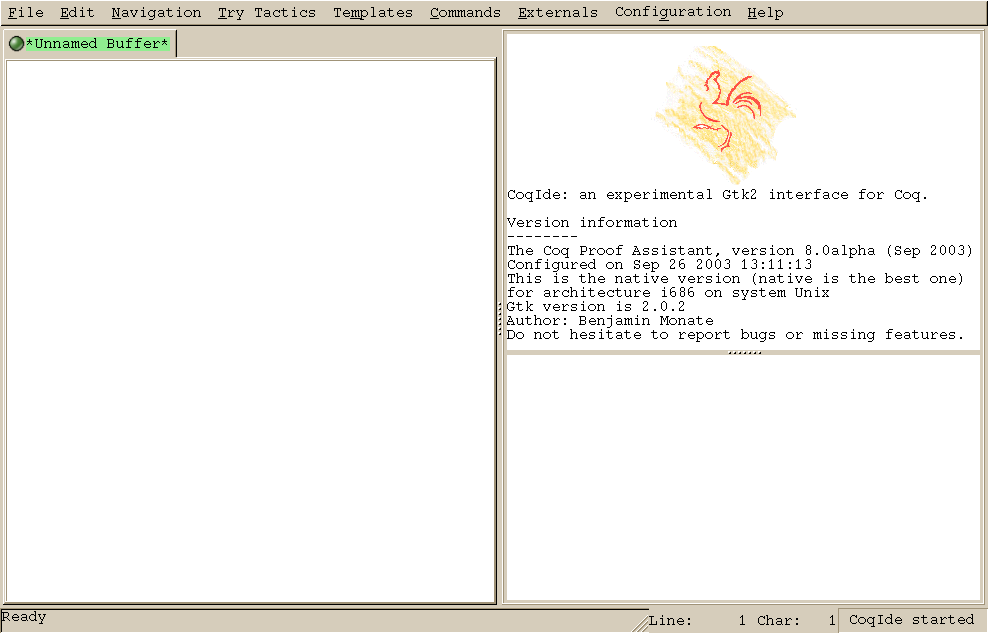
\includegraphics[width=1.0\textwidth]{coqide.png}
\else
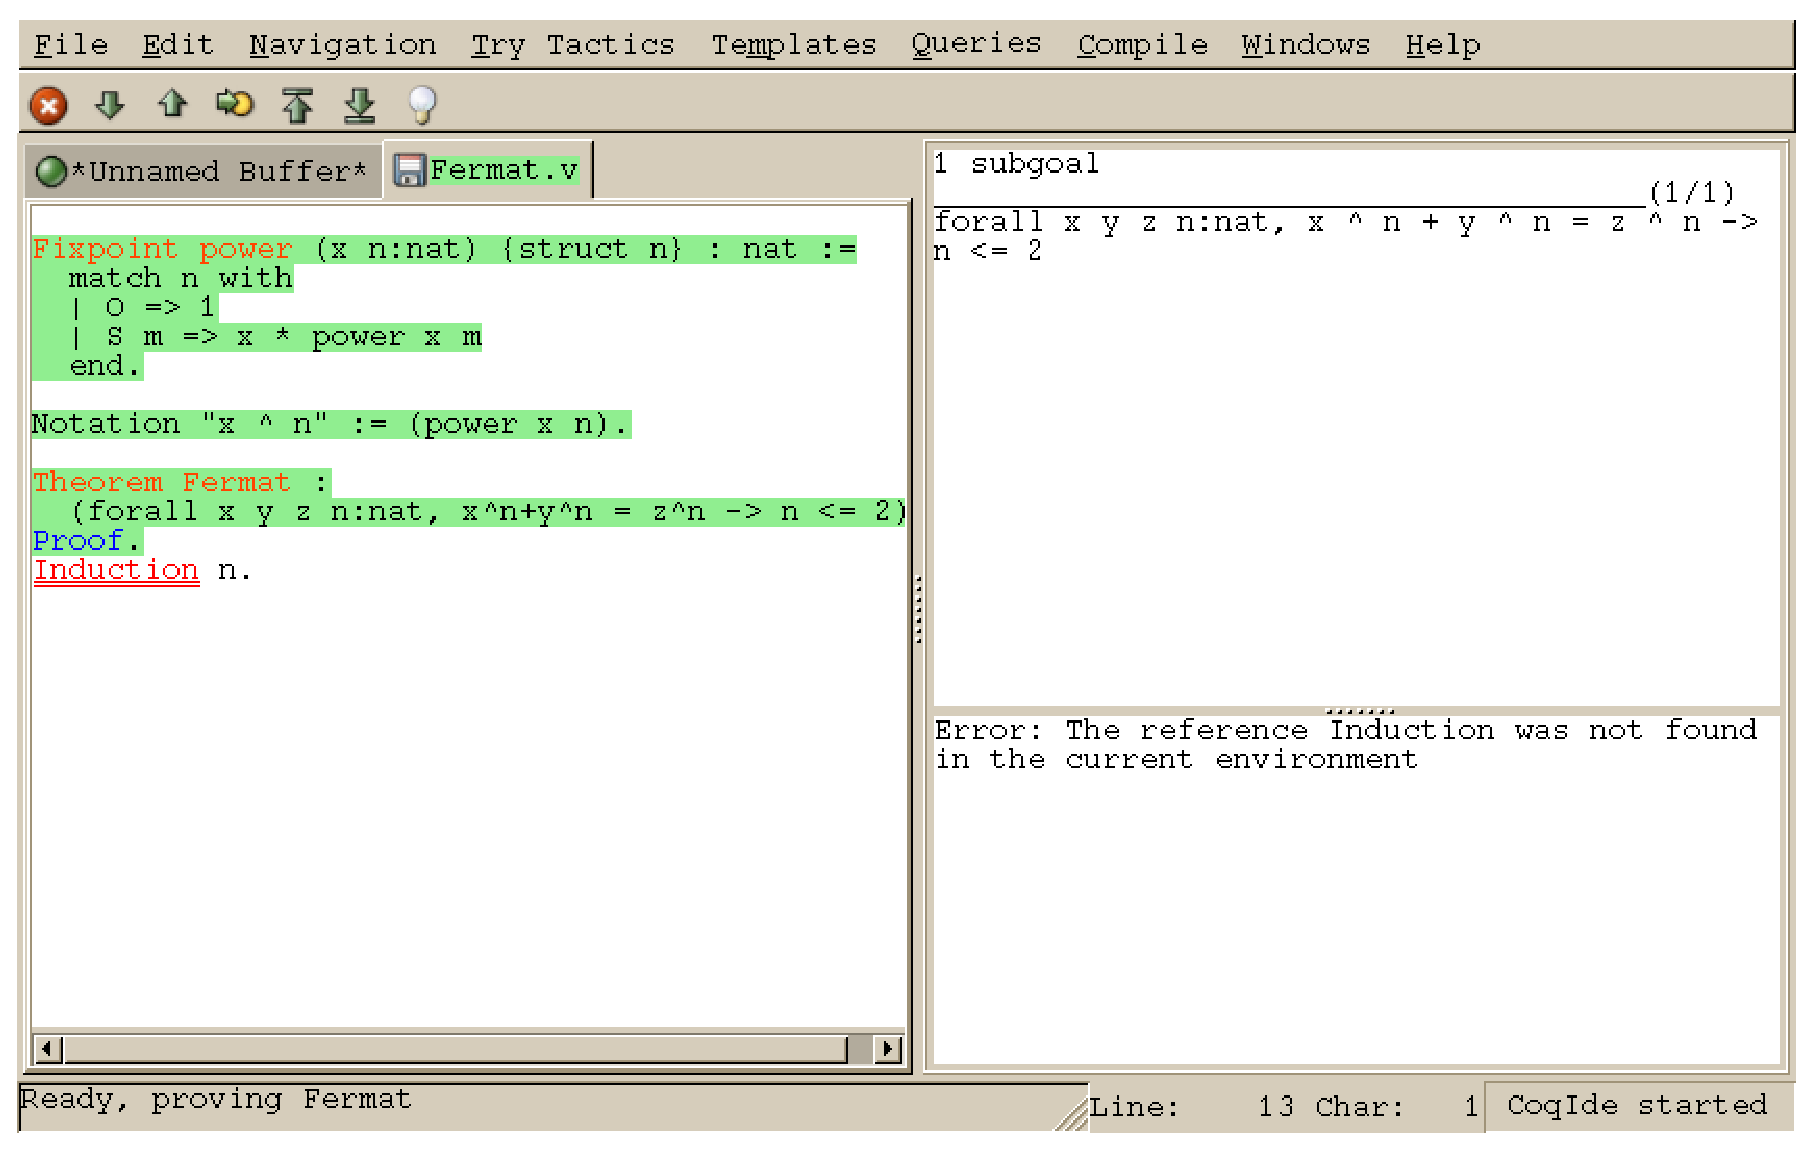
\includegraphics[width=1.0\textwidth]{coqide.eps}
\fi
%END LATEX
\end{center}
\caption{\CoqIDE{} main screen}
\label{fig:coqide}
\end{figure}

A sample \CoqIDE{} main screen, while navigating into a file
\verb|Fermat.v|, is shown on Figure~\ref{fig:coqide}.  At
the top is a menu bar, and a tool bar below it. The large window on
the left is displaying the various \emph{script buffers}. The upper right
window is the \emph{goal window}, where goals to 
prove are displayed. The lower right window is the \emph{message window},
where various messages resulting from commands are displayed. At the
bottom is the status bar.

\section{Managing files and buffers, basic edition}

In the script window, you may open arbitrarily many buffers to
edit. The \emph{File} menu allows you to open files or create some,
save them, print or export them into various formats. Among all these
buffers, there is always one which is the current \emph{running
  buffer}, whose name is displayed on a green background, which is the
one where Coq commands are currently executed. 

Buffers may be edited as in any text editor, and classical basic
editing commands (Copy/Paste, \ldots) are available in the \emph{Edit}
menu. \CoqIDE{} offers only basic editing commands, so if you need
more complex editing commands, you may launch your favorite text
editor on the current buffer, using the \emph{Edit/External Editor}
menu. 

\section{Interactive navigation into \Coq{} scripts}

The running buffer is the one where navigation takes place. The
toolbar proposes five basic commands for this. The first one,
represented by a down arrow icon, is for going forward executing one
command. If that command is successful, the part of the script that
has been executed is displayed on a green background. If that command
fails, the error message is displayed in the message window, and the
location of the error is emphasized by a red underline.

On Figure~\ref{fig:coqide}, the running buffer is \verb|Fermat.v|, all
commands until the \verb|Theorem| have been already executed, and the
user tried to go forward executing \verb|Induction n|. That command
failed because no such tactic exist (tactics are now in
lowercase\ldots), and the wrong word is underlined. 

Notice that the green part of the running buffer is not editable. If
you ever want to modify something you have to go backward using the up
arrow tool, or even better, put the cursor where you want to go back
and use the \textsf{goto} button. Unlike with \verb|coqtop|, you
should never use \verb|Undo| to go backward.

Two additional tool buttons exist, one to go directly to the end and
one to go back to the beginning. If you try to go to the end, or in
general to run several commands using the \textsf{goto} button, the
  execution will stop whenever an error is found.

If you ever try to execute a command which happens to run during a
long time, and would like to abort it before its
termination, you may use the interrupt button (the white cross on a red circle).
 
Finally, notice that these navigation buttons are also available in
the menu, where their keyboard shortcuts are given.

\section[Try tactics automatically]{Try tactics automatically\label{sec:trytactics}}

The menu \texttt{Try Tactics} provides some features for automatically
trying to solve the current goal using simple tactics. If such a
tactic succeeds in solving the goal, then its text is automatically
inserted into the script. There is finally a combination of these
tactics, called the \emph{proof wizard} which will try each of them in
turn. This wizard is also available as a tool button (the light
bulb).  The set of tactics tried by the wizard is customizable in
the preferences.

These tactics are general ones, in particular they do not refer to
particular hypotheses. You may also try specific tactics related to
the goal or one of the hypotheses, by clicking with the right mouse
button on the goal or the considered hypothesis. This is the
``contextual menu on goals'' feature, that may be disabled in the
preferences if undesirable.

\section{Proof folding}

As your script grows bigger and bigger, it might be useful to hide the proofs
of your theorems and lemmas.

This feature is toggled via the \texttt{Hide} entry of the \texttt{Navigation}
menu. The proof shall be enclosed between \texttt{Proof.} and \texttt{Qed.},
both with their final dots. The proof that shall be hidden or revealed is the
first one whose beginning statement (such as \texttt{Theorem}) precedes the
insertion cursor.
 
\section{Vernacular commands, templates}

The \texttt{Templates} menu allows to use shortcuts to insert
vernacular commands. This is a nice way to proceed if you are not sure
of the spelling of the command you want.

Moreover, this menu offers some \emph{templates} which will automatic
insert a complex command like Fixpoint with a convenient shape for its
arguments. 

\section{Queries}

\begin{figure}[t]
\begin{center}
%HEVEA\imgsrc{coqide-queries.png}
%BEGIN LATEX
\ifpdf  % si on est en pdflatex
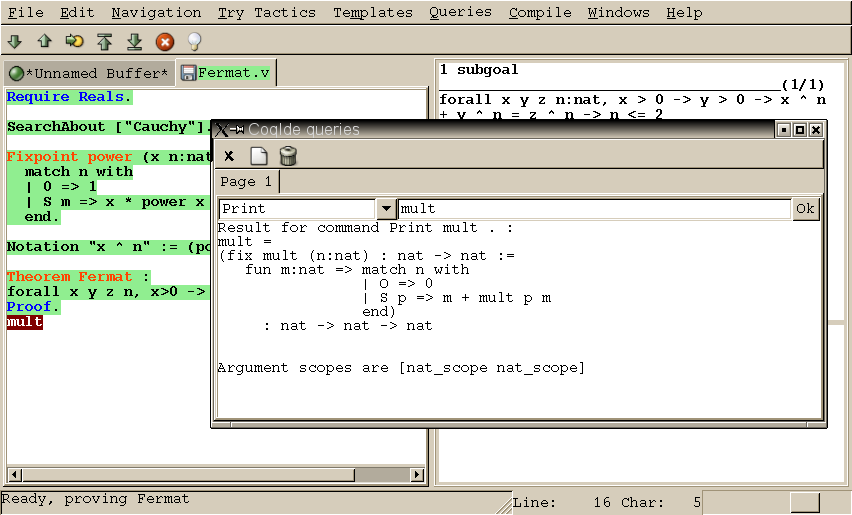
\includegraphics[width=1.0\textwidth]{coqide-queries.png}
\else
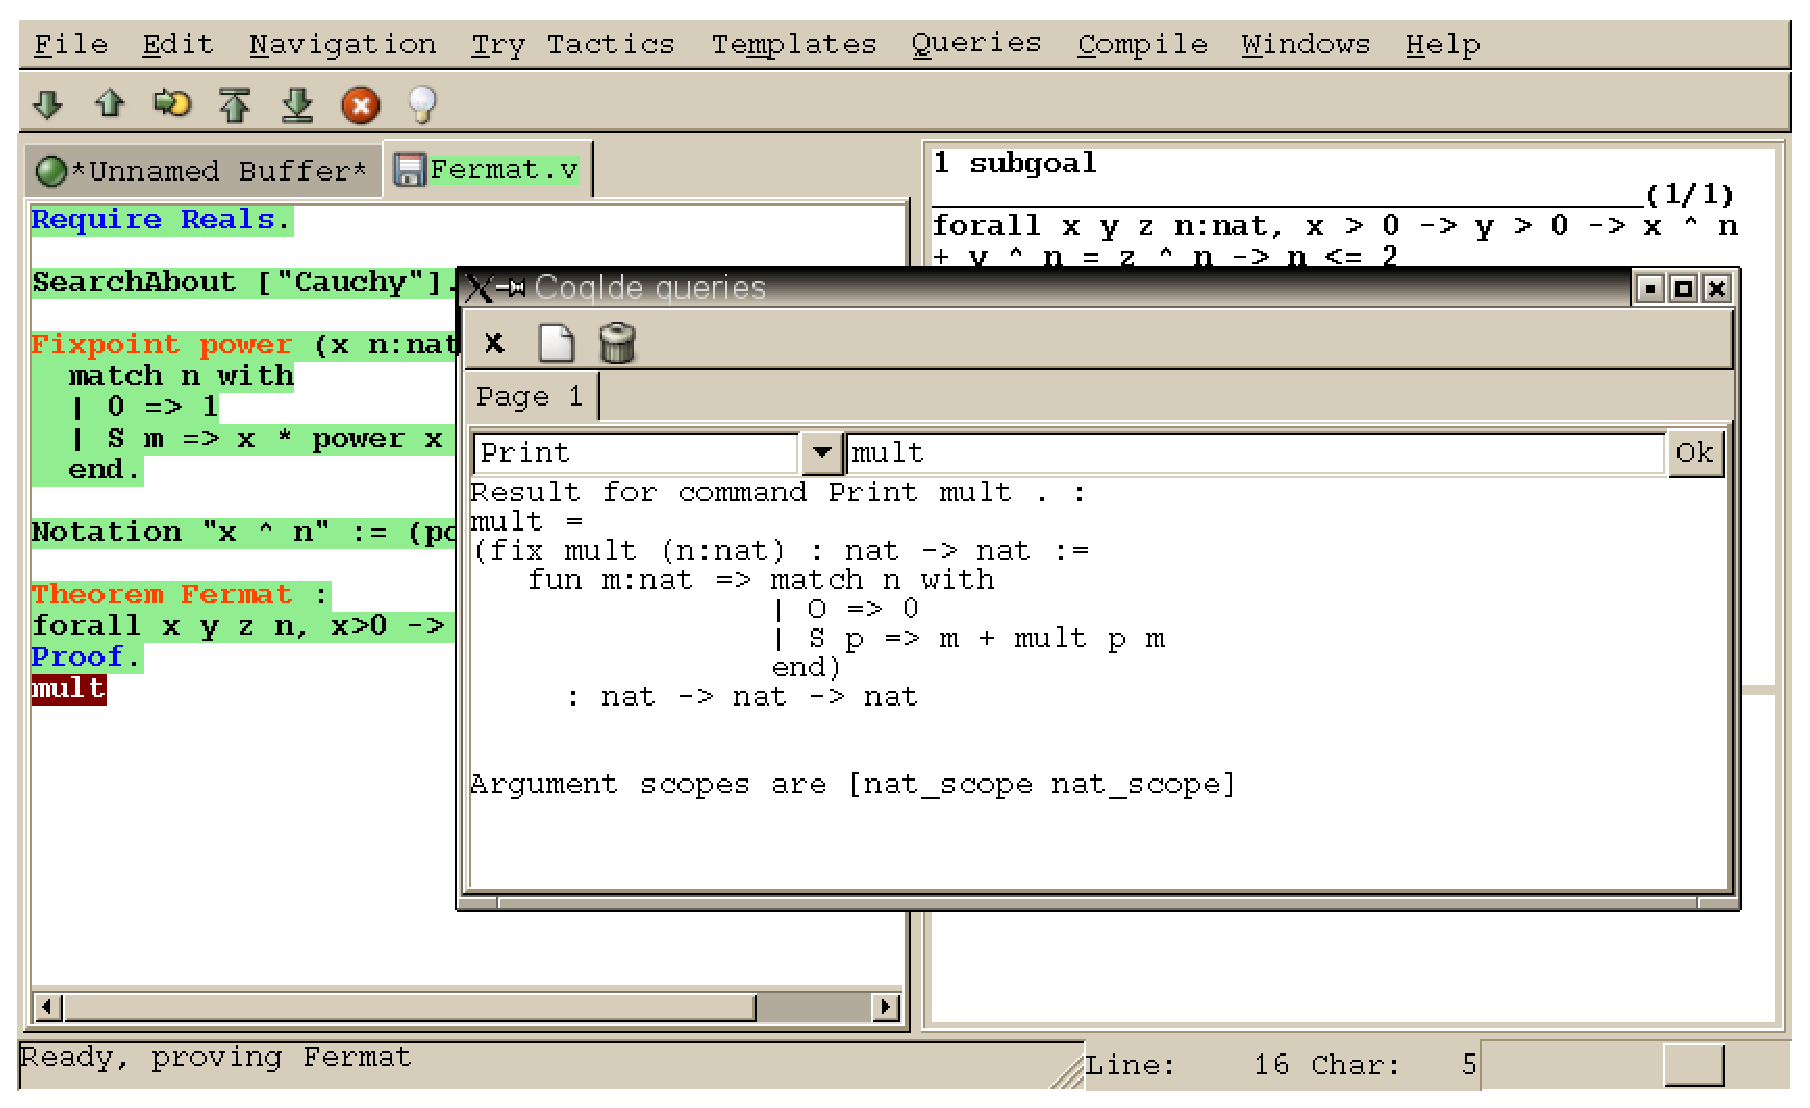
\includegraphics[width=1.0\textwidth]{coqide-queries.eps}
\fi
%END LATEX
\end{center}
\caption{\CoqIDE{}: the query window}
\label{fig:querywindow}
\end{figure}


We call \emph{query} any vernacular command that do not change the
current state, such as \verb|Check|, \verb|SearchAbout|, etc. Those
commands are of course useless during compilation of a file, hence
should not be included in scripts. To run such commands without
writing them in the script, \CoqIDE{} offers another input window
called the \emph{query window}. This window can be displayed on
demand, either by using the \texttt{Window} menu, or directly using
shortcuts given in the \texttt{Queries} menu. Indeed, with \CoqIDE{}
the simplest way to perform a \texttt{SearchAbout} on some identifier
is to select it using the mouse, and pressing \verb|F2|. This will
both make appear the query window and run the \texttt{SearchAbout} in
it, displaying the result. Shortcuts \verb|F3| and \verb|F4| are for
\verb|Check| and \verb|Print| respectively.
Figure~\ref{fig:querywindow} displays the query window after selection
of the word ``mult'' in the script windows, and pressing \verb|F4| to
print its definition.

\section{Compilation}

The \verb|Compile| menu offers direct commands to:
\begin{itemize}
\item compile the current buffer
\item run a compilation using \verb|make|
\item go to the last compilation error
\item create a \verb|makefile| using \verb|coq_makefile|.
\end{itemize}

\section{Customizations}

You may customize your environment using menu
\texttt{Edit/Preferences}. A new window will be displayed, with
several customization sections presented as a notebook. 

The first section is for selecting the text font used for scripts, goal
and message windows. 

The second section is devoted to file management: you may
configure automatic saving of files, by periodically saving the
contents into files named \verb|#f#| for each opened file
\verb|f|. You may also activate the \emph{revert} feature: in case a
opened file is modified on the disk by a third party, \CoqIDE{} may read
it again for you. Note that in the case you edited that same file, you
will be prompt to choose to either discard your changes or not. The
\texttt{File charset encoding} choice is described below in
Section~\ref{sec:coqidecharencoding}
 

The \verb|Externals| section allows to customize the external commands
for compilation, printing, web browsing. In the browser command, you
may use \verb|%s| to denote the URL to open, for example: %
\verb|mozilla -remote "OpenURL(%s)"|. 

The \verb|Tactics Wizard| section allows to defined the set of tactics
that should be tried, in sequence, to solve the current goal.

The last section is for miscellaneous boolean settings, such as the
``contextual menu on goals'' feature presented in
Section~\ref{sec:trytactics}. 

Notice that these settings are saved in the file \verb|.coqiderc| of
your home directory. 

A gtk2 accelerator keymap is saved under the name \verb|.coqide.keys|.
This file should not be edited manually: to modify a given menu
shortcut, go to the corresponding menu item without releasing the
mouse button, press the key you want for the new shortcut, and release
the mouse button afterwards.

For experts: it is also possible to set up a specific gtk resource
file, under the name \verb|.coqide-gtk2rc|, following the gtk2
resources syntax
\url{http://developer.gnome.org/doc/API/2.0/gtk/gtk-Resource-Files.html}.
Such a default resource file can be found in the subdirectory
\verb=lib/coq/ide= of the root installation directory of \Coq{}
(alternatively, it can be found in the subdirectory \verb=ide= of the
source archive of \Coq{}). You may
copy this file into your home directory, and edit it using any text
editor, \CoqIDE{} itself for example.

\section{Using unicode symbols}

\CoqIDE{} supports unicode character encoding in its text windows,
consequently a large set of symbols is available for notations.

\subsection{Displaying unicode symbols}

You just need to define suitable notations as described in
Chapter~\ref{Addoc-syntax}. For example, to use the mathematical symbols
$\forall$ and $\exists$, you may define 
\begin{quote}\tt
Notation "$\forall$ x : t, P" := \\
\qquad  (forall x:t, P) (at level 200, x ident).\\
Notation "$\exists$ x : t, P" := \\
\qquad  (exists x:t, P) (at level 200, x ident).
\end{quote}
There exists a small set of such notations already defined, in the
file \verb|utf8.v| of \Coq{} library, so you may enable them just by 
\verb|Require utf8| inside \CoqIDE{}, or equivalently, by starting
\CoqIDE{} with \verb|coqide -l utf8|.

However, there are some issues when using such unicode symbols: you of
course need to use a character font which supports them. In the Fonts
section of the preferences, the Preview line displays some unicode symbols, so
you could figure out if the selected font is OK. Related to this, one
thing you may need to do is choose whether Gtk should use antialiased
fonts or not, by setting the environment variable \verb|GDK_USE_XFT|
to 1 or 0 respectively.

\subsection{Defining an input method for non ASCII symbols}

To input an Unicode symbol, a general method is to press both the
CONTROL and the SHIFT keys, and type the hexadecimal code of the
symbol required, for example \verb|2200| for the $\forall$ symbol.
A list of symbol codes is available at \url{http://www.unicode.org}. 

This method obviously doesn't scale, that's why the preferred alternative is to
use an Input Method Editor. On POSIX systems (Linux distros, BSD variants and
MacOS X), you can use \texttt{uim} version 1.6 or later which provides a \LaTeX{}-style
input method.

To configure \texttt{uim}, execute \texttt{uim-pref-gtk} as your regular user.
In the "Global Settings" group set the default Input Method to "ELatin" (don't
forget to tick the checkbox "Specify default IM"). In the "ELatin" group set the
layout to "TeX", and remember the content of the "[ELatin] on" field (by default
"<Control>\textbackslash"). You can now execute CoqIDE with the following commands (assuming
you use a Bourne-style shell):

\begin{verbatim}
$ export GTK_IM_MODULE=uim
$ coqide
\end{verbatim}

Activate the ELatin Input Method with Ctrl-\textbackslash, then type the
sequence "\verb=\Gamma=". You will see the sequence being
replaced by $\Gamma$ as soon as you type the second "a".

\subsection[Character encoding for saved files]{Character encoding for saved files\label{sec:coqidecharencoding}}

In the \texttt{Files} section of the preferences, the encoding option
is related to the way files are saved. 

If you have no need to exchange files with non UTF-8 aware
applications, it is better to choose the UTF-8 encoding, since it
guarantees that your files will be read again without problems. (This
is because when \CoqIDE{} reads a file, it tries to automatically
detect its character encoding.) 

If you choose something else than UTF-8, then missing characters will
be written encoded by \verb|\x{....}| or \verb|\x{........}| where
each dot is an hexadecimal digit: the number between braces is the
hexadecimal UNICODE index for the missing character.


%%% Local Variables: 
%%% mode: latex
%%% TeX-master: "Reference-Manual"
%%% End: 
% Coq IDE

%BEGIN LATEX
\RefManCutCommand{BEGINADDENDUM=\thepage}
%END LATEX
\part{Addendum to the Reference Manual}
%\coverpage{Addendum to the Reference Manual}{\ }
%\addcontentsline{toc}{part}{Additional documentation}
%BEGIN LATEX
\setheaders{Presentation of the Addendum}
%END LATEX
\chapter*{Presentation of the Addendum}

Here you will find several pieces of additional documentation for the
\Coq\ Reference Manual. Each of this chapters is concentrated on a
particular topic, that should interest only a fraction of the \Coq\
users: that's the reason why they are apart from the Reference
Manual.

\begin{description}

\item[Extended pattern-matching] This chapter details the use of
  generalized pattern-matching. It is contributed by Cristina Cornes
  and Hugo Herbelin.

\item[Implicit coercions] This chapter details the use of the coercion
  mechanism.  It is contributed by Amokrane Sa�bi.

%\item[Proof of imperative programs] This chapter explains how to
%  prove properties of annotated programs with imperative features.
%  It is contributed by Jean-Christophe Filli�tre

\item[Program extraction] This chapter explains how to extract in practice ML
  files from $\FW$ terms.   It is contributed by Jean-Christophe
  Filli�tre and Pierre Letouzey.

%\item[Natural] This chapter is due to Yann Coscoy. It is the user
%  manual of the tools he wrote for printing proofs in natural
%  language. At this time, French and English languages are supported.

\item[omega] \texttt{omega}, written by Pierre Cr�gut, solves a whole
  class of arithmetic problems.

%\item[Program] The \texttt{Program} technology intends to inverse the
%  extraction mechanism. It allows the developments of certified
%  programs in \Coq. This chapter is due to Catherine Parent. {\bf This
%  feature is not available in {\Coq} version 7.}

\item[The {\tt ring} tactic] This is a tactic to do AC rewriting. This
  chapter explains how to use it and how it works.
  The chapter is contributed by Patrick Loiseleur.

\item[The {\tt Setoid\_replace} tactic] This is a
  tactic to do rewriting on types equipped with specific (only partially
  substitutive) equality. The chapter is contributed by Cl�ment Renard.


\end{description}

\atableofcontents


%%% Local Variables: 
%%% mode: latex
%%% TeX-master: "Reference-Manual"
%%% End: 
%
\achapter{Extended pattern-matching}
%BEGIN LATEX
\defaultheaders
%END LATEX
\aauthor{Cristina Cornes and Hugo Herbelin}

\label{Mult-match-full}
\ttindex{Cases}
\index{ML-like patterns}

This section describes the full form of pattern-matching in {\Coq} terms.

\asection{Patterns}\label{implementation} The full syntax of {\tt
match} is presented in Figures~\ref{term-syntax}
and~\ref{term-syntax-aux}.  Identifiers in patterns are either
constructor names or variables. Any identifier that is not the
constructor of an inductive or co-inductive type is considered to be a
variable. A variable name cannot occur more than once in a given
pattern. It is recommended to start variable names by a lowercase
letter.

If a pattern has the form $(c~\vec{x})$ where $c$ is a constructor
symbol and $\vec{x}$ is a linear vector of (distinct) variables, it is
called {\em simple}: it is the kind of pattern recognized by the basic
version of {\tt match}. On the opposite, if it is a variable $x$ or
has the form $(c~\vec{p})$ with $p$ not only made of variables, the
pattern is called {\em nested}.

A variable pattern matches any value, and the identifier is bound to
that value. The pattern ``\texttt{\_}'' (called ``don't care'' or
``wildcard'' symbol) also matches any value, but does not bind
anything. It may occur an arbitrary number of times in a
pattern. Alias patterns written \texttt{(}{\sl pattern} \texttt{as}
{\sl identifier}\texttt{)} are also accepted. This pattern matches the
same values as {\sl pattern} does and {\sl identifier} is bound to the
matched value.  
A pattern of the form {\pattern}{\tt |}{\pattern} is called
disjunctive. A list of patterns separated with commas is also
considered as a pattern and is called {\em multiple pattern}. However
multiple patterns can only occur at the root of pattern-matching
equations. Disjunctions of {\em multiple pattern} are allowed though.

Since extended {\tt match} expressions are compiled into the primitive
ones, the expressiveness of the theory remains the same. Once the
stage of parsing has finished only simple patterns remain.  Re-nesting
of pattern is performed at printing time. An easy way to see the
result of the expansion is to toggle off the nesting performed at
printing (use here {\tt Set Printing Matching}), then by printing the term
with \texttt{Print} if the term is a constant, or using the command
\texttt{Check}.

The extended \texttt{match} still accepts an optional {\em elimination
predicate} given after the keyword \texttt{return}.  Given a pattern
matching expression, if all the right-hand-sides of \texttt{=>} ({\em
rhs} in short) have the same type, then this type can be sometimes
synthesized, and so we can omit the \texttt{return} part. Otherwise 
the predicate after \texttt{return} has to be provided, like for the basic
\texttt{match}.

Let us illustrate through examples the different aspects of extended
pattern matching. Consider for example the function that computes the
maximum of two natural numbers. We can write it in primitive syntax
by:

\begin{coq_example}
Fixpoint max (n m:nat) {struct m} : nat :=
  match n with
  | O => m
  | S n' => match m with
            | O => S n'
            | S m' => S (max n' m')
            end
  end.
\end{coq_example}

\paragraph{Multiple patterns}

Using multiple patterns in the definition of {\tt max} allows to write:

\begin{coq_example}
Reset max.
Fixpoint max (n m:nat) {struct m} : nat :=
  match n, m with
  | O, _ => m
  | S n', O => S n'
  | S n', S m' => S (max n' m')
  end.
\end{coq_example}

which will be compiled into the previous form.

The pattern-matching compilation strategy examines patterns from left
to right. A \texttt{match} expression is generated {\bf only} when
there is at least one constructor in the column of patterns. E.g. the
following example does not build a \texttt{match} expression.

\begin{coq_example}
Check (fun x:nat => match x return nat with
                    | y => y
                    end).
\end{coq_example}

\paragraph{Aliasing subpatterns}

We can also use ``\texttt{as} {\ident}'' to associate a name to a
sub-pattern:

\begin{coq_example}
Reset max.
Fixpoint max (n m:nat) {struct n} : nat :=
  match n, m with
  | O, _ => m
  | S n' as p, O => p
  | S n', S m' => S (max n' m')
  end.
\end{coq_example}

\paragraph{Nested patterns}

Here is now an example of nested patterns:

\begin{coq_example}
Fixpoint even (n:nat) : bool :=
  match n with
  | O => true
  | S O => false
  | S (S n') => even n'
  end.
\end{coq_example}

This is compiled into:

\begin{coq_example}
Unset Printing Matching.
Print even.
Set Printing Matching.
\end{coq_example}

In the previous examples patterns do not conflict with, but
sometimes it is comfortable to write patterns that admit a non
trivial superposition. Consider
the boolean function \texttt{lef} that given two natural numbers
yields \texttt{true} if the first one is less or equal than the second
one and \texttt{false} otherwise. We can write it as follows:

\begin{coq_example}
Fixpoint lef (n m:nat) {struct m} : bool :=
  match n, m with
  | O, x => true
  | x, O => false
  | S n, S m => lef n m
  end.
\end{coq_example}

Note that the first and the second multiple pattern superpose because
the couple of values \texttt{O O} matches both. Thus, what is the result
of the function on those values?  To eliminate ambiguity we use the
{\em textual priority rule}: we consider patterns ordered from top to
bottom, then a value is matched by the pattern at the $ith$ row if and
only if it is not matched by some pattern of a previous row. Thus in the
example,
\texttt{O O} is matched by the first pattern, and so \texttt{(lef O O)}
yields \texttt{true}.

Another way to write  this function is:

\begin{coq_example}
Reset lef.
Fixpoint lef (n m:nat) {struct m} : bool :=
  match n, m with
  | O, x => true
  | S n, S m => lef n m
  | _, _ => false
  end.
\end{coq_example}

Here the last pattern superposes with the first two. Because
of the priority rule, the last pattern 
will be used only for values that do not match neither the  first nor
the second one.  

Terms with useless patterns are not accepted by the
system. Here is an example:
% Test failure
\begin{coq_eval}
Set Printing Depth 50.
  (********** The following is not correct and should produce **********)
  (**************** Error: This clause is redundant ********************)
\end{coq_eval}
\begin{coq_example}
Check (fun x:nat =>
         match x with
         | O => true
         | S _ => false
         | x => true
         end).
\end{coq_example}

\paragraph{Disjunctive patterns}

Multiple patterns that share the same right-hand-side can be
factorized using the notation \nelist{\multpattern}{\tt |}. For instance,
{\tt max} can be rewritten as follows:

\begin{coq_eval}
Reset max.
\end{coq_eval}
\begin{coq_example}
Fixpoint max (n m:nat) {struct m} : nat :=
  match n, m with
  | S n', S m' => S (max n' m')
  | 0, p | p, 0 => p
  end.
\end{coq_example}

Similarly, factorization of (non necessary multiple) patterns
that share the same variables is possible by using the notation
\nelist{\pattern}{\tt |}. Here is an example:

\begin{coq_example}
Definition filter_2_4 (n:nat) : nat :=
  match n with
  | 2 as m | 4 as m => m
  | _ => 0
  end.
\end{coq_example}

Here is another example using disjunctive subpatterns.

\begin{coq_example}
Definition filter_some_square_corners (p:nat*nat) : nat*nat :=
  match p with
  | ((2 as m | 4 as m), (3 as n | 5 as n)) => (m,n)
  | _ => (0,0)
  end.
\end{coq_example}

\asection{About patterns of parametric types}
\paragraph{Parameters in patterns}
When matching objects of a parametric type, parameters do not bind in patterns.
They must be substituted by ``\_''.
Consider for example the type of polymorphic lists:

\begin{coq_example}
Inductive List (A:Set) : Set :=
  | nil : List A
  | cons : A -> List A -> List A.
\end{coq_example}

We can check the function {\em tail}:

\begin{coq_example}
Check
  (fun l:List nat =>
     match l with
     | nil _ => nil nat
     | cons _ _ l' => l'
     end).
\end{coq_example}


When we use parameters in patterns there is an error message:
% Test failure
\begin{coq_eval}
Set Printing Depth 50.
(********** The following is not correct and should produce **********)
(******** Error: Parameters do not bind ... ************)
\end{coq_eval}
\begin{coq_example}
Check
  (fun l:List nat =>
     match l with
     | nil A => nil nat
     | cons A _ l' => l'
     end).
\end{coq_example}

\paragraph{Implicit arguments in patterns}
By default, implicit arguments are omitted in patterns. So we write:

\begin{coq_example}
Arguments nil [A].
Arguments cons [A] _ _.
Check
  (fun l:List nat =>
     match l with
     | nil => nil
     | cons _ l' => l'
     end).
\end{coq_example}

But the possibility to use all the arguments is given by ``{\tt @}'' implicit
explicitations (as for terms~\ref{Implicits-explicitation}).

\begin{coq_example}
Check
  (fun l:List nat =>
     match l with
     | @nil _ => @nil nat
     | @cons _ _ l' => l'
     end).
\end{coq_example}

\asection{Matching objects of dependent types}
The previous examples illustrate pattern matching on objects of
non-dependent types, but we can also 
use the expansion strategy to destructure objects of dependent type.
Consider the type \texttt{listn} of lists of a certain length:
\label{listn}

\begin{coq_example}
Inductive listn : nat -> Set :=
  | niln : listn 0
  | consn : forall n:nat, nat -> listn n -> listn (S n).
\end{coq_example}

\asubsection{Understanding dependencies in patterns}
We can define the function \texttt{length} over \texttt{listn} by:

\begin{coq_example}
Definition length (n:nat) (l:listn n) := n.
\end{coq_example}

Just for illustrating pattern matching, 
we can define it by case analysis:

\begin{coq_example}
Reset length.
Definition length (n:nat) (l:listn n) :=
  match l with
  | niln => 0
  | consn n _ _ => S n
  end.
\end{coq_example}

We can understand the meaning of this definition using the
same notions of usual pattern matching.

%
% Constraining of dependencies is not longer valid in V7
%
\iffalse
Now suppose we split the second pattern  of \texttt{length} into two 
cases so to give an
alternative definition using nested patterns:
\begin{coq_example}
Definition length1 (n:nat) (l:listn n) :=
  match l with
  | niln => 0
  | consn n _ niln => S n
  | consn n _ (consn _ _ _) => S n
  end.
\end{coq_example}

It is obvious that \texttt{length1} is  another version of
\texttt{length}. We can also give the following definition:
\begin{coq_example}
Definition length2 (n:nat) (l:listn n) :=
  match l with
  | niln => 0
  | consn n _ niln => 1
  | consn n _ (consn m _ _) => S (S m)
  end.
\end{coq_example}

If we forget that \texttt{listn} is a dependent type and we read these
definitions using the usual semantics of pattern matching,  we can conclude
that \texttt{length1}
and \texttt{length2} are different functions.
In fact, they are equivalent
because the pattern \texttt{niln} implies that \texttt{n} can only match
the value $0$ and analogously the pattern \texttt{consn} determines that \texttt{n} can
only match  values of the form  $(S~v)$ where $v$ is the value matched by
\texttt{m}. 

The converse is also true. If
we destructure the  length  value with the pattern \texttt{O} then the list
value should be $niln$. 
Thus, the following term \texttt{length3} corresponds to the function
\texttt{length} but this time defined by case analysis on the dependencies instead of on the list:

\begin{coq_example}
Definition length3 (n:nat) (l:listn n) :=
  match l with
  | niln => 0
  | consn O _ _ => 1
  | consn (S n) _ _ => S (S n)
  end.
\end{coq_example}

When we have nested patterns of dependent types, the semantics of
pattern matching becomes a little more difficult because
the set of values that are matched by a sub-pattern may be conditioned by the
values matched by another sub-pattern. Dependent nested patterns are
somehow constrained patterns. 
In the examples, the expansion of
\texttt{length1} and \texttt{length2} yields exactly the same term
 but the
expansion of \texttt{length3} is completely different. \texttt{length1} and
\texttt{length2} are expanded into two nested case analysis on
\texttt{listn} while \texttt{length3} is expanded into a case analysis on
\texttt{listn} containing a case analysis on natural numbers inside.


In practice the user can think about the patterns as independent and
it is the expansion algorithm that cares to relate them. \\
\fi
%
%
%

\asubsection{When the elimination predicate must be provided}
\paragraph{Dependent pattern matching}
The examples  given so far do not need an explicit elimination predicate
 because all the rhs have the same type and the
strategy succeeds to synthesize it.
Unfortunately when dealing with dependent patterns it often happens
that we need to write cases where the type of the rhs are 
different  instances of the elimination  predicate.
The function  \texttt{concat} for \texttt{listn}
is an example where the branches have different type
and we need to provide the elimination predicate:

\begin{coq_example}
Fixpoint concat (n:nat) (l:listn n) (m:nat) (l':listn m) {struct l} :
 listn (n + m) :=
  match l in listn n return listn (n + m) with
  | niln => l'
  | consn n' a y => consn (n' + m) a (concat n' y m l')
  end.
\end{coq_example}
The elimination predicate is {\tt fun (n:nat) (l:listn n) => listn~(n+m)}.
In general if $m$ has type $(I~q_1\ldots q_r~t_1\ldots t_s)$ where 
$q_1\ldots q_r$ are parameters, the elimination predicate should be of
the form~:
{\tt fun $y_1$\ldots $y_s$ $x$:($I$~$q_1$\ldots $q_r$~$y_1$\ldots
  $y_s$) => Q}.

In the concrete syntax, it should be written~:
\[ \kw{match}~m~\kw{as}~x~\kw{in}~(I~\_\ldots \_~y_1\ldots y_s)~\kw{return}~Q~\kw{with}~\ldots~\kw{end}\]

The variables which appear in the \kw{in} and \kw{as} clause are new
and bounded in the property $Q$ in the \kw{return} clause. The
parameters of the inductive definitions should not be mentioned and
are replaced by \kw{\_}.

\paragraph{Multiple dependent pattern matching}
Recall that a list of patterns is also a pattern. So, when we destructure several
terms at the same time and the branches have different types we need to provide the
elimination predicate for this multiple pattern. It is done using the same
scheme, each term may be associated to an \kw{as} and \kw{in} clause in order to
introduce a dependent product.

For example, an equivalent definition for \texttt{concat} (even though the
matching on the second term is trivial) would have been:

\begin{coq_example}
Reset concat.
Fixpoint concat (n:nat) (l:listn n) (m:nat) (l':listn m) {struct l} :
 listn (n + m) :=
  match l in listn n, l' return listn (n + m) with
  | niln, x => x
  | consn n' a y, x => consn (n' + m) a (concat n' y m x)
  end.
\end{coq_example}

Even without real matching over the second term, this construction can be used to
keep types linked.  If {\tt a} and {\tt b} are two {\tt listn} of the same length,
by writing
\begin{coq_eval}
  Unset Printing Matching.
\end{coq_eval}
\begin{coq_example}
Check (fun n (a b: listn n) => match a,b with
 |niln,b0 => tt
 |consn n' a y, bS => tt
end).
\end{coq_example}
\begin{coq_eval}
  Set Printing Matching.
\end{coq_eval}

I have a copy of {\tt b} in type {\tt listn 0} resp {\tt listn (S n')}.

% Notice that this time, the predicate \texttt{[n,\_:nat](listn (plus n
%   m))}  is binary because we
% destructure both \texttt{l} and \texttt{l'} whose types have arity one.
% In general, if we destructure the terms $e_1\ldots e_n$
% the predicate will be of arity $m$ where $m$ is the sum of the
% number of dependencies of the type of $e_1, e_2,\ldots e_n$
% (the $\lambda$-abstractions
% should correspond from left to right to each dependent argument of the
% type of $e_1\ldots e_n$).
% When the arity of the predicate (i.e. number of abstractions) is not
% correct Coq raises an error message. For example:

% % Test failure
% \begin{coq_eval}
% Reset concat.
% Set Printing Depth 50.
% (********** The following is not correct and should produce ***********)
% (** Error: the term l' has type listn m while it is expected to have **)
% (** type listn (?31 + ?32)                                           **)
% \end{coq_eval}
% \begin{coq_example}
% Fixpoint concat
%  (n:nat) (l:listn n) (m:nat)
%  (l':listn m) {struct l} : listn (n + m) :=
%   match l, l' with
%   | niln, x => x
%   | consn n' a y, x => consn (n' + m) a (concat n' y m x)
%   end.
% \end{coq_example}

\paragraph{Patterns in {\tt in}}
If the type of the matched term is more precise than an inductive applied to
variables, arguments of the inductive in the {\tt in} branch can be more
complicated patterns than a variable.

Moreover, constructors whose type do not follow the same pattern will become
impossible branch. In impossible branch, you can answer anything but {\tt
  False\_rect unit} has the advantage to be subterm of anything.

To be concrete: the tail function can be written:
\begin{coq_example}
  Definition tail n (v: listn (S n)) :=
    match v in listn (S m) return listn m with
      | niln => False_rect unit
      | consn n' a y => y
    end.
\end{coq_example}
and {\tt tail n v} will be subterm of {\tt v}.

\asection{Using pattern matching to write proofs}
In all the previous examples the elimination predicate does not depend
on the object(s) matched. But it may depend and the typical case 
is when we write a proof by induction or a function that yields an
object of dependent type. An example of proof using \texttt{match} in
given in Section~\ref{refine-example}.

For example, we can write 
the function \texttt{buildlist} that given a natural number
$n$ builds a list of length $n$ containing zeros as follows:

\begin{coq_example}
Fixpoint buildlist (n:nat) : listn n :=
  match n return listn n with
  | O => niln
  | S n => consn n 0 (buildlist n)
  end.
\end{coq_example}

We can also use multiple patterns. 
Consider the following definition of the predicate less-equal
\texttt{Le}:

\begin{coq_example}
Inductive LE : nat -> nat -> Prop :=
  | LEO : forall n:nat, LE 0 n
  | LES : forall n m:nat, LE n m -> LE (S n) (S m).
\end{coq_example}

We can use multiple patterns to write  the proof of the lemma
 \texttt{forall (n m:nat), (LE n m)}\verb=\/=\texttt{(LE m n)}:

\begin{coq_example}
Fixpoint dec (n m:nat) {struct n} : LE n m \/ LE m n :=
  match n, m return LE n m \/ LE m n with
  | O, x => or_introl (LE x 0) (LEO x)
  | x, O => or_intror (LE x 0) (LEO x)
  | S n as n', S m as m' =>
      match dec n m with
      | or_introl h => or_introl (LE m' n') (LES n m h)
      | or_intror h => or_intror (LE n' m') (LES m n h)
      end
  end.
\end{coq_example}
In the example of \texttt{dec},
the first \texttt{match} is dependent while 
the second is not.

% In general, consider the terms $e_1\ldots e_n$,
% where  the type of $e_i$ is an instance of a family type
% $\lb (\vec{d_i}:\vec{D_i}) \mto T_i$  ($1\leq i
% \leq n$). Then, in expression \texttt{match}  $e_1,\ldots,
% e_n$ \texttt{of} \ldots \texttt{end}, the 
% elimination predicate ${\cal P}$ should be of the form:
% $[\vec{d_1}:\vec{D_1}][x_1:T_1]\ldots [\vec{d_n}:\vec{D_n}][x_n:T_n]Q.$

The user can also use \texttt{match} in combination with the tactic
\texttt{refine} (see Section~\ref{refine}) to build incomplete proofs
beginning with a \texttt{match} construction.

\asection{Pattern-matching on inductive objects involving local
definitions}

If local definitions occur in the type of a constructor, then there are two ways
to match on this constructor. Either the local definitions are skipped and
matching is done only on the true arguments of the constructors, or the bindings
for local definitions can also be caught in the matching.

Example.

\begin{coq_eval}
Reset Initial.
Require Import Arith.
\end{coq_eval}

\begin{coq_example*}
Inductive list : nat -> Set :=
  | nil : list 0
  | cons : forall n:nat, let m := (2 * n) in list m -> list (S (S m)).
\end{coq_example*}

In the next example, the local definition is not caught.

\begin{coq_example}
Fixpoint length n (l:list n) {struct l} : nat :=
  match l with
  | nil => 0
  | cons n l0 => S (length (2 * n) l0)
  end.
\end{coq_example}

But in this example, it is.

\begin{coq_example}
Fixpoint length' n (l:list n) {struct l} : nat :=
  match l with
  | nil => 0
  | @cons _ m l0 => S (length' m l0)
  end.
\end{coq_example}

\Rem for a given matching clause, either none of the local definitions or all of
them can be caught.

\Rem you can only catch {\tt let} bindings in mode where you bind all variables and so you
have to use @ syntax.

\Rem this feature is incoherent with the fact that parameters cannot be caught and
consequently is somehow hidden. For example, there is no mention of it in error messages.

\asection{Pattern-matching and coercions}

If a mismatch occurs between the expected type of a pattern and its
actual type, a coercion made from constructors is sought. If such a
coercion can be found, it is automatically inserted around the
pattern.

Example:

\begin{coq_example}
Inductive I : Set :=
  | C1 : nat -> I
  | C2 : I -> I.
Coercion C1 : nat >-> I.
Check (fun x => match x with
                | C2 O => 0
                | _ => 0
                end).
\end{coq_example}


\asection{When does the expansion strategy fail ?}\label{limitations}
The strategy works very like in ML languages when treating
patterns of non-dependent type.  
But there are new cases of failure that are due to the presence of 
dependencies. 

The error messages of the current implementation may be sometimes
confusing.  When the tactic fails because patterns are somehow
incorrect then error messages refer to the initial expression. But the
strategy may succeed to build an expression whose sub-expressions are
well typed when the whole expression is not. In this situation the
message makes reference to the expanded expression.  We encourage
users, when they have patterns with the same outer constructor in
different equations, to name the variable patterns in the same
positions with the same name.  
E.g. to write {\small\texttt{(cons n O x) => e1}} 
and {\small\texttt{(cons n \_ x) => e2}} instead of
{\small\texttt{(cons n O x) => e1}} and 
{\small\texttt{(cons n' \_ x') => e2}}. 
This helps to maintain certain name correspondence between the
generated expression and the original.

Here is a summary of the error messages corresponding to each situation:

\begin{ErrMsgs}
\item \sverb{The constructor } {\sl
    ident} \sverb{ expects } {\sl num} \sverb{ arguments}
  
 \sverb{The variable } {\sl ident} \sverb{ is bound several times
    in pattern } {\sl term}
  
 \sverb{Found a constructor of inductive type } {\term}
 \sverb{ while a constructor of } {\term} \sverb{ is expected}

 Patterns are incorrect (because constructors are not applied to
  the correct number of the arguments, because they are not linear or
  they are wrongly typed).

\item \errindex{Non exhaustive pattern-matching}

The pattern matching is not exhaustive.

\item \sverb{The elimination predicate } {\sl term} \sverb{ should be
    of arity } {\sl num} \sverb{ (for non dependent case) or } {\sl
    num} \sverb{ (for dependent case)}

The elimination predicate provided to \texttt{match} has not the
  expected arity.


%\item the whole expression is wrongly typed

% CADUC ?
% , or the synthesis of
%   implicit arguments fails (for example to find the elimination
%   predicate or to resolve implicit arguments in the rhs).
 
%   There are {\em nested patterns of dependent type}, the elimination
%   predicate corresponds to non-dependent case and has the form
%   $[x_1:T_1]...[x_n:T_n]T$ and {\bf some} $x_i$ occurs {\bf free} in
%   $T$.  Then, the strategy may fail to find out a correct elimination
%   predicate during some step of compilation.  In this situation we
%   recommend the user to rewrite the nested dependent patterns into
%   several \texttt{match} with {\em simple patterns}.
  
\item {\tt Unable to infer a match predicate\\
    Either there is a type incompatiblity or the problem involves\\
    dependencies}
 
  There is a type mismatch between the different branches.
  The user should provide an elimination predicate.

% Obsolete ?  
% \item because of nested patterns, it may happen that even though all
%   the rhs have the same type, the strategy needs dependent elimination
%   and so an elimination predicate must be provided. The system warns
%   about this situation, trying to compile anyway with the
%   non-dependent strategy. The risen message is:

% \begin{itemize}
% \item {\tt Warning: This pattern matching may need dependent
%     elimination to be compiled.  I will try, but if fails try again
%     giving dependent elimination predicate.}
% \end{itemize}


%%%%%%%%%%%%%%%%%%%%%%%%%%%%%%%%%%%%%%%%%%%%%%%%%%%%%%%%%%%%%%%%%%%%%%
% % LA PROPAGATION DES CONTRAINTES ARRIERE N'EST PAS FAITE DANS LA V7
% TODO
% \item there are {\em nested patterns of dependent type} and the
%   strategy builds a term that is well typed but recursive calls in fix
%   point are reported as illegal:
% \begin{itemize}
% \item {\tt Error: Recursive call applied to an illegal term ...}
% \end{itemize}

% This is because the strategy generates a term that is correct w.r.t.
% the initial term but which does not pass the guard condition.  In
% this situation we recommend the user to transform the nested dependent
% patterns into {\em several \texttt{match} of simple patterns}.  Let us
% explain this with an example.  Consider the following definition of a
% function that yields the last element of a list and \texttt{O} if it is
% empty:

% \begin{coq_example}
%   Fixpoint last [n:nat; l:(listn n)] : nat :=
%    match l of 
%      (consn _ a niln) => a
%    | (consn m _ x) => (last m x) | niln => O
%    end.
% \end{coq_example}

% It fails because of the priority between patterns, we know that this
% definition is equivalent to the following more explicit one (which
% fails too):

% \begin{coq_example*}
%   Fixpoint last [n:nat; l:(listn n)] : nat :=
%    match l of
%      (consn _ a niln) => a
%    | (consn n _ (consn m b x)) => (last n (consn m b x))
%    | niln => O
%    end.
% \end{coq_example*}

% Note that the recursive call {\tt (last n (consn m b x))} is not
% guarded. When treating with patterns of dependent types the strategy
% interprets the first definition of \texttt{last} as the second
% one\footnote{In languages of the ML family the first definition would
%   be translated into a term where the variable \texttt{x} is shared in
%   the expression.  When patterns are of non-dependent types, Coq
%   compiles as in ML languages using sharing. When patterns are of
%   dependent types the compilation reconstructs the term as in the
%   second definition of \texttt{last} so to ensure the result of
%   expansion is well typed.}.  Thus it generates a term where the
% recursive call is rejected by the guard condition.

% You can get rid of this problem by writing the definition with
% \emph{simple patterns}:

% \begin{coq_example}
%   Fixpoint last [n:nat; l:(listn n)] : nat :=
%   <[_:nat]nat>match l of
%     (consn m a x) => Cases x of niln => a | _ => (last m x) end
%   | niln => O
%   end.
% \end{coq_example}

\end{ErrMsgs}


%%% Local Variables: 
%%% mode: latex
%%% TeX-master: "Reference-Manual"
%%% End: 
%
\achapter{Implicit Coercions}
%HEVEA\cutname{coercions.html}
\aauthor{Amokrane Saïbi}

\label{Coercions-full}
\index{Coercions!presentation}

\asection{General Presentation}

This section describes the inheritance mechanism of {\Coq}. In {\Coq} with
inheritance, we are not interested in adding any expressive power to
our theory, but only convenience. Given a term, possibly not typable,
we are interested in the problem of determining if it can be well
typed modulo insertion of appropriate coercions.  We allow to write:

\begin{itemize}
\item $f~a$ where $f:forall~ x:A, B$ and $a:A'$ when $A'$ can 
      be seen in some sense as a subtype of $A$.
\item $x:A$ when $A$ is not a type, but can be seen in 
      a certain sense as a type: set, group, category etc.
\item $f~a$ when $f$ is not a function, but can be seen in a certain sense
      as a function: bijection, functor, any structure morphism etc.
\end{itemize}

\asection{Classes}
\index{Coercions!classes}
 A class with $n$ parameters is any defined name with a type
$forall~ (x_1:A_1)..(x_n:A_n), s$ where $s$ is a sort.  Thus a class with
parameters is considered as a single class and not as a family of
classes.  An object of a class $C$ is any term of type $C~t_1
.. t_n$.  In addition to these user-classes, we have two abstract
classes:

\begin{itemize}
\item {\tt Sortclass}, the class of sorts; 
  its objects are the terms whose type is a sort (e.g., \texttt{Prop}
  or \texttt{Type}).
\item {\tt Funclass}, the class of functions; 
  its objects are all the terms with a functional 
  type, i.e. of form $forall~ x:A, B$.
\end{itemize}

Formally, the syntax of a classes is defined on Figure~\ref{fig:classes}.
\begin{figure}
\begin{centerframe}
\begin{tabular}{lcl}
{\class} & ::= & {\qualid} \\
  & $|$ & {\tt Sortclass} \\
  & $|$ & {\tt Funclass} 
\end{tabular}
\end{centerframe}
\caption{Syntax of classes}
\label{fig:classes}
\end{figure}

\asection{Coercions}
\index{Coercions!Funclass}
\index{Coercions!Sortclass}
  A name $f$ can be declared as a coercion between a source user-class
$C$ with $n$ parameters and a target class $D$ if one of these
conditions holds:

\newcommand{\oftype}{\!:\!}

\begin{itemize}
\item $D$ is a user-class, then the type of $f$ must have the form
      $forall~ (x_1 \oftype A_1)..(x_n \oftype A_n)(y\oftype C~x_1..x_n), D~u_1..u_m$ where $m$
      is the number of parameters of $D$.
\item $D$ is {\tt Funclass}, then the type of $f$ must have the form
      $forall~ (x_1\oftype A_1)..(x_n\oftype A_n)(y\oftype C~x_1..x_n)(x:A), B$. 
\item $D$ is {\tt Sortclass}, then the type of $f$ must have the form
      $forall~ (x_1\oftype A_1)..(x_n\oftype A_n)(y\oftype C~x_1..x_n), s$ with $s$ a sort. 
\end{itemize}

We then write $f:C \mbox{\texttt{>->}} D$. The restriction on the type
of coercions is called {\em the uniform inheritance condition}.
Remark: the abstract class {\tt Sortclass} can be used as source class,
but the abstract class {\tt Funclass} cannot.

To coerce an object $t:C~t_1..t_n$ of $C$ towards $D$, we have to
apply the coercion $f$ to it; the obtained term $f~t_1..t_n~t$ is
then an object of $D$.

\asection{Identity Coercions}
\index{Coercions!identity}

  Identity coercions are special cases of coercions used to go around
the uniform inheritance condition.  Let $C$ and $D$ be two classes
with respectively $n$ and $m$ parameters and
$f:forall~(x_1:T_1)..(x_k:T_k)(y:C~u_1..u_n), D~v_1..v_m$ a function which
does not verify the uniform inheritance condition. To declare $f$ as
coercion, one has first to declare a subclass $C'$ of $C$:

$$C' := fun~ (x_1:T_1)..(x_k:T_k) => C~u_1..u_n$$

\noindent We then define an {\em identity coercion} between $C'$ and $C$:
\begin{eqnarray*}
Id\_C'\_C  & := & fun~ (x_1:T_1)..(x_k:T_k)(y:C'~x_1..x_k) => (y:C~u_1..u_n)\\
\end{eqnarray*}

We can now declare $f$ as coercion from $C'$ to $D$, since we can
``cast'' its type as
$forall~ (x_1:T_1)..(x_k:T_k)(y:C'~x_1..x_k),D~v_1..v_m$.\\ The identity
coercions have a special status: to coerce an object $t:C'~t_1..t_k$
of $C'$ towards $C$, we does not have to insert explicitly $Id\_C'\_C$
since $Id\_C'\_C~t_1..t_k~t$ is convertible with $t$.  However we
``rewrite'' the type of $t$ to become an object of $C$; in this case,
it becomes $C~u_1^*..u_k^*$ where each $u_i^*$ is the result of the
substitution in $u_i$ of the variables $x_j$ by $t_j$.


\asection{Inheritance Graph}
\index{Coercions!inheritance graph}
Coercions form an inheritance graph with classes as nodes.  We call
{\em coercion path} an ordered list of coercions between two nodes of
the graph.  A class $C$ is said to be a subclass of $D$ if there is a
coercion path in the graph from $C$ to $D$; we also say that $C$
inherits from $D$. Our mechanism supports multiple inheritance since a
class may inherit from several classes, contrary to simple inheritance
where a class inherits from at most one class.  However there must be
at most one path between two classes.  If this is not the case, only
the {\em oldest} one is valid and the others are ignored. So the order
of declaration of coercions is important.

We extend notations for coercions to coercion paths. For instance
$[f_1;..;f_k]:C \mbox{\texttt{>->}} D$ is the coercion path composed
by the coercions $f_1..f_k$.  The application of a coercion path to a
term consists of the successive application of its coercions.

\asection{Declaration of Coercions}

%%%%% "Class" is useless, since classes are implicitely defined via coercions.

% \asubsection{\tt Class {\qualid}.}\comindex{Class}
% Declares {\qualid} as a new class.

% \begin{ErrMsgs}
% \item {\qualid} \errindex{not declared}
% \item {\qualid} \errindex{is already a class}
% \item \errindex{Type of {\qualid} does not end with a sort}
% \end{ErrMsgs}

% \begin{Variant}
% \item {\tt Class Local {\qualid}.} \\
% Declares the construction denoted by {\qualid} as a new local class to 
% the current section.
% \end{Variant}

% END "Class" is useless

\asubsection{\tt Coercion {\qualid} : {\class$_1$} >-> {\class$_2$}.}
\comindex{Coercion}

Declares the construction denoted by {\qualid} as a coercion between
{\class$_1$} and {\class$_2$}.

% Useless information
% The classes {\class$_1$} and {\class$_2$} are first declared if necessary.
   
\begin{ErrMsgs}
\item {\qualid} \errindex{not declared}
\item {\qualid} \errindex{is already a coercion}
\item \errindex{Funclass cannot be a source class}
\item {\qualid} \errindex{is not a function}
\item \errindex{Cannot find the source class of {\qualid}}
\item \errindex{Cannot recognize {\class$_1$} as a source class of {\qualid}}
\item {\qualid} \errindex{does not respect the uniform inheritance condition}
\item \errindex{Found target class {\class} instead of {\class$_2$}}

\end{ErrMsgs}

When the coercion {\qualid} is added to the inheritance graph, non
valid coercion paths are ignored; they are signaled by a warning.
\\[0.3cm]
\noindent {\bf Warning :}
\begin{enumerate}
\item \begin{tabbing}
{\tt Ambiguous paths: }\= $[f_1^1;..;f_{n_1}^1] : C_1\mbox{\tt >->}D_1$\\
                       \> {\ldots} \\
                       \>$[f_1^m;..;f_{n_m}^m] : C_m\mbox{\tt >->}D_m$
      \end{tabbing}
\end{enumerate}

\begin{Variants}
\item {\tt Local Coercion {\qualid} : {\class$_1$} >-> {\class$_2$}.}
\comindex{Local Coercion}\\
  Declares the construction denoted by {\qualid} as a coercion local to
  the current section.

\item {\tt Coercion {\ident} := {\term}}\comindex{Coercion}\\
  This defines {\ident} just like \texttt{Definition {\ident} :=
    {\term}}, and then declares {\ident} as a coercion between it
  source and its target.

\item {\tt Coercion {\ident} := {\term} : {\type}}\\
  This defines {\ident} just like 
  \texttt{Definition {\ident} : {\type} := {\term}}, and then
  declares {\ident} as a coercion between it source and its target. 

\item {\tt Local Coercion {\ident} := {\term}}\comindex{Local Coercion}\\
  This defines {\ident} just like \texttt{Let {\ident} :=
    {\term}}, and then declares {\ident} as a coercion between it
  source and its target.

\item Assumptions can be declared as coercions at declaration
time. This extends the grammar of assumptions from 
Figure~\ref{sentences-syntax} as follows:
\comindex{Variable \mbox{\rm (and coercions)}}
\comindex{Axiom \mbox{\rm (and coercions)}}
\comindex{Parameter \mbox{\rm (and coercions)}}
\comindex{Hypothesis \mbox{\rm (and coercions)}}

\begin{tabular}{lcl}
%% Declarations
{\assumption} & ::= & {\assumptionkeyword} {\assums} {\tt .} \\
&&\\
{\assums} & ::= & {\simpleassums} \\
          & $|$ & \nelist{{\tt (} \simpleassums {\tt )}}{} \\
&&\\
{\simpleassums} & ::= &  \nelist{\ident}{} {\tt :}\zeroone{{\tt >}} {\term}\\  
\end{tabular}

If the extra {\tt >} is present before the type of some assumptions, these
assumptions are declared as coercions.

\item Constructors of inductive types can be declared as coercions at
definition time of the inductive type. This extends and modifies the
grammar of inductive types from Figure \ref{sentences-syntax} as follows: 
\comindex{Inductive \mbox{\rm (and coercions)}}
\comindex{CoInductive \mbox{\rm (and coercions)}}

\begin{center}
\begin{tabular}{lcl}
%% Inductives
{\inductive} & ::= & 
           {\tt Inductive} \nelist{\inductivebody}{with} {\tt .} \\
 & $|$ & {\tt CoInductive} \nelist{\inductivebody}{with} {\tt .} \\
           & & \\
{\inductivebody} & ::= & 
  {\ident} \zeroone{\binders} {\tt :} {\term} {\tt :=} \\
   && ~~~\zeroone{\zeroone{\tt |} \nelist{\constructor}{|}} \\
           & & \\
{\constructor} & ::= &  {\ident} \zeroone{\binders} \zeroone{{\tt :}\zeroone{\tt >} {\term}} \\
\end{tabular}
\end{center}

Especially, if the extra {\tt >} is present in a constructor
declaration, this constructor is declared as a coercion.
\end{Variants}

\asubsection{\tt Identity Coercion {\ident}:{\class$_1$} >-> {\class$_2$}.} 
\comindex{Identity Coercion}

We check that {\class$_1$} is a constant with a value of the form
$fun~ (x_1:T_1)..(x_n:T_n) => (\mbox{\class}_2~t_1..t_m)$ where $m$ is the
number of parameters of \class$_2$.  Then we define an identity
function with the type
$forall~ (x_1:T_1)..(x_n:T_n)(y:\mbox{\class}_1~x_1..x_n),
{\mbox{\class}_2}~t_1..t_m$, and we declare it as an identity
coercion between {\class$_1$} and {\class$_2$}.

\begin{ErrMsgs}
\item {\class$_1$} \errindex{must be a transparent constant} 
\end{ErrMsgs}

\begin{Variants}
\item {\tt Local Identity Coercion {\ident}:{\ident$_1$} >-> {\ident$_2$}.} \\
Idem but locally to the current section.

\item {\tt SubClass {\ident} := {\type}.} \\
\comindex{SubClass}
 If {\type} is a class
{\ident'} applied to some arguments then {\ident} is defined and an
identity coercion of name {\tt Id\_{\ident}\_{\ident'}} is
declared. Otherwise said, this is an abbreviation for 

{\tt Definition {\ident} := {\type}.} 

 followed by

{\tt Identity Coercion Id\_{\ident}\_{\ident'}:{\ident} >-> {\ident'}}.

\item {\tt Local SubClass {\ident} := {\type}.} \\
Same as before but locally to the current section.

\end{Variants}

\asection{Displaying Available Coercions}

\asubsection{\tt Print Classes.} 
\comindex{Print Classes}
Print the list of declared classes in the current context.

\asubsection{\tt Print Coercions.}
\comindex{Print Coercions}
Print the list of declared coercions in the current context.

\asubsection{\tt Print Graph.} 
\comindex{Print Graph}
Print the list of valid coercion paths in the current context.

\asubsection{\tt Print Coercion Paths {\class$_1$} {\class$_2$}.} 
\comindex{Print Coercion Paths}
Print the list of valid coercion paths from {\class$_1$} to {\class$_2$}.

\asection{Activating the Printing of Coercions}

\asubsection{\tt Set Printing Coercions.}
\optindex{Printing Coercions}

This command forces all the coercions to be printed.
Conversely, to skip the printing of coercions, use
 {\tt Unset Printing Coercions}.
By default, coercions are not printed.

\asubsection{\tt Add Printing Coercion {\qualid}.}
\comindex{Add Printing Coercion}
\comindex{Remove Printing Coercion}

This command forces coercion denoted by {\qualid} to be printed.
To skip the printing of coercion {\qualid}, use
 {\tt Remove Printing Coercion {\qualid}}.
By default, a coercion is never printed.
 
\asection{Classes as Records}
\label{Coercions-and-records}
\index{Coercions!and records}
We allow the definition of {\em Structures with Inheritance} (or
classes as records) by extending the existing {\tt Record} macro
(see Section~\ref{Record}). Its new syntax is:

\begin{center}
\begin{tabular}{l}
{\tt Record \zeroone{>}~{\ident} \zeroone{\binders} : {\sort} := \zeroone{\ident$_0$} \verb+{+} \\
~~~~\begin{tabular}{l}
        {\tt \ident$_1$ $[$:$|$:>$]$ \term$_1$ ;} \\
        ... \\
        {\tt \ident$_n$ $[$:$|$:>$]$ \term$_n$ \verb+}+. }
    \end{tabular}
\end{tabular}
\end{center}
The identifier {\ident} is the name of the defined record and {\sort}
is its type. The identifier {\ident$_0$} is the name of its
constructor. The identifiers {\ident$_1$}, .., {\ident$_n$} are the
names of its fields and {\term$_1$}, .., {\term$_n$} their respective
types. The alternative {\tt $[$:$|$:>$]$} is ``{\tt :}'' or ``{\tt
:>}''. If {\tt {\ident$_i$}:>{\term$_i$}}, then {\ident$_i$} is
automatically declared as coercion from {\ident} to the class of
{\term$_i$}.  Remark that {\ident$_i$} always verifies the uniform
inheritance condition.  If the optional ``{\tt >}'' before {\ident} is
present, then {\ident$_0$} (or the default name {\tt Build\_{\ident}}
if {\ident$_0$} is omitted) is automatically declared as a coercion
from the class of {\term$_n$} to {\ident} (this may fail if the
uniform inheritance condition is not satisfied).

\Rem The keyword {\tt Structure}\comindex{Structure} is a synonym of {\tt
Record}.

\asection{Coercions and Sections}
\index{Coercions!and sections}
  The inheritance mechanism is compatible with the section
mechanism. The global classes and coercions defined inside a section
are redefined after its closing, using their new value and new
type. The classes and coercions which are local to the section are
simply forgotten.
Coercions with a local source class or a local target class, and 
coercions which do not verify the uniform inheritance condition any longer
are also forgotten.

\asection{Coercions and Modules}
\index{Coercions!and modules}

From Coq version 8.3, the coercions present in a module are activated
only when the module is explicitly imported. Formerly, the coercions
were activated as soon as the module was required, whatever it was
imported or not.

To recover the behavior of the versions of Coq prior to 8.3, use the
following command:

\optindex{Automatic Coercions Import}
\begin{verbatim}
Set Automatic Coercions Import.
\end{verbatim}

To cancel the effect of the option, use instead:

\begin{verbatim}
Unset Automatic Coercions Import.
\end{verbatim}

\asection{Examples}

  There are three situations:

\begin{itemize}
\item $f~a$ is ill-typed where $f:forall~x:A,B$ and $a:A'$. If there is a
      coercion path between $A'$ and $A$, $f~a$ is transformed into
      $f~a'$ where $a'$ is the result of the application of this
      coercion path to $a$.

We first give an example of coercion between atomic inductive types

%\begin{\small}
\begin{coq_example}
Definition bool_in_nat (b:bool) := if b then 0 else 1.
Coercion bool_in_nat : bool >-> nat.
Check (0 = true).
Set Printing Coercions.
Check (0 = true).
\end{coq_example}
%\end{small}

\begin{coq_eval}
Unset Printing Coercions.
\end{coq_eval}

\Warning ``\verb|Check true=O.|'' fails. This is ``normal'' behaviour of
coercions. To validate \verb|true=O|, the coercion is searched from
\verb=nat= to \verb=bool=. There is none.

We give an example of coercion between classes with parameters.

%\begin{\small}
\begin{coq_example}
Parameters
   (C : nat -> Set) (D : nat -> bool -> Set) (E : bool -> Set).
Parameter f : forall n:nat, C n -> D (S n) true.
Coercion f : C >-> D.
Parameter g : forall (n:nat) (b:bool), D n b -> E b.
Coercion g : D >-> E.
Parameter c : C 0.
Parameter T : E true -> nat.
Check (T c).
Set Printing Coercions.
Check (T c).
\end{coq_example}
%\end{small}

\begin{coq_eval}
Unset Printing Coercions.
\end{coq_eval}

We give now an example using identity coercions.

%\begin{small}
\begin{coq_example}
Definition D' (b:bool) := D 1 b.
Identity Coercion IdD'D : D' >-> D.
Print IdD'D.
Parameter d' : D' true.
Check (T d').
Set Printing Coercions.
Check (T d').
\end{coq_example}
%\end{small}

\begin{coq_eval}
Unset Printing Coercions.
\end{coq_eval}


  In the case of functional arguments, we use the monotonic rule of
sub-typing.  Approximatively, to coerce $t:forall~x:A, B$ towards
$forall~x:A',B'$, one have to coerce $A'$ towards $A$ and $B$ towards
$B'$. An example is given below:

%\begin{small}
\begin{coq_example}
Parameters (A B : Set) (h : A -> B).
Coercion h : A >-> B.
Parameter U : (A -> E true) -> nat.
Parameter t : B -> C 0.
Check (U t).
Set Printing Coercions.
Check (U t).
\end{coq_example}
%\end{small}

\begin{coq_eval}
Unset Printing Coercions.
\end{coq_eval}

  Remark the changes in the result following the modification of the
previous example.

%\begin{small}
\begin{coq_example}
Parameter U' : (C 0 -> B) -> nat.
Parameter t' : E true -> A.
Check (U' t').
Set Printing Coercions.
Check (U' t').
\end{coq_example}
%\end{small}

\begin{coq_eval}
Unset Printing Coercions.
\end{coq_eval}

\item An assumption $x:A$ when $A$ is not a type, is ill-typed.  It is
      replaced by $x:A'$ where $A'$ is the result of the application
      to $A$ of the coercion path between the class of $A$ and {\tt
      Sortclass} if it exists.  This case occurs in the abstraction
      $fun~ x:A => t$, universal quantification $forall~x:A, B$,
      global variables and parameters of (co-)inductive definitions
      and functions. In $forall~x:A, B$, such a coercion path may be
      applied to $B$ also if necessary.

%\begin{small}
\begin{coq_example}
Parameter Graph : Type.
Parameter Node : Graph -> Type.
Coercion Node : Graph >-> Sortclass.
Parameter G : Graph.
Parameter Arrows : G -> G -> Type.
Check Arrows.
Parameter fg : G -> G.
Check fg.
Set Printing Coercions.
Check fg.
\end{coq_example}
%\end{small}

\begin{coq_eval}
Unset Printing Coercions.
\end{coq_eval}

\item $f~a$ is ill-typed because $f:A$ is not a function. The term
      $f$ is replaced by the term obtained by applying to $f$ the
      coercion path between $A$ and {\tt Funclass} if it exists.

%\begin{small}
\begin{coq_example}
Parameter bij : Set -> Set -> Set.
Parameter ap : forall A B:Set, bij A B -> A -> B.
Coercion ap : bij >-> Funclass.
Parameter b : bij nat nat.
Check (b 0).
Set Printing Coercions.
Check (b 0).
\end{coq_example}
%\end{small}

\begin{coq_eval}
Unset Printing Coercions.
\end{coq_eval}

Let us see the resulting graph of this session.

%\begin{small}
\begin{coq_example}
Print Graph.
\end{coq_example}
%\end{small}

\end{itemize}


%%% Local Variables: 
%%% mode: latex
%%% TeX-master: "Reference-Manual"
%%% End: 
%
%%SUPPRIME \achapter{\texttt{Natural} : proofs in natural language}
\aauthor{Yann Coscoy}

\asection{Introduction}

\Natural~ is a package allowing the writing of proofs in natural
language. For instance, the proof in \Coq~of the induction principle on pairs
of natural numbers looks like this:

\begin{coq_example*}
Require Natural.
\end{coq_example*}
\begin{coq_example}
Print nat_double_ind.
\end{coq_example}

Piping it through the \Natural~pretty-printer gives:

\comindex{Print Natural}
\begin{coq_example}
Print Natural nat_double_ind.
\end{coq_example}

\asection{Activating \Natural}

To enable the printing of proofs in natural language, you should
type under \texttt{coqtop} or \texttt{coqtop -full} the command

\begin{coq_example*}
Require Natural.
\end{coq_example*}

By default, proofs are transcripted in english. If you wish to print them 
in French, set the French option by

\comindex{Set Natural}
\begin{coq_example*}
Set Natural French.
\end{coq_example*}

If you want to go back to English, type in

\begin{coq_example*}
Set Natural English.
\end{coq_example*}

Currently, only \verb=French= and \verb=English= are available.

You may see for example the natural transcription of the proof of
the induction principle on pairs of natural numbers:

\begin{coq_example*}
Print Natural nat_double_ind.
\end{coq_example*}

You may  also show in natural language the current proof in progress:

\comindex{Show Natural}
\begin{coq_example}
Goal (n:nat)(le O n).
Induction n.
Show Natural Proof.
\end{coq_example}

\subsection*{Restrictions}

For \Natural, a proof is an object of type a proposition (i.e. an
object of type something of type {\tt Prop}). Only proofs are written
in natural language when typing {\tt Print Natural \ident}.  All other
objects (the objects of type something which is of type {\tt Set} or
{\tt Type}) are written as usual $\lambda$-terms.

\asection{Customizing \Natural}

The transcription of proofs in natural language is mainly a paraphrase of
the formal proofs, but some specific hints in the transcription
can be given.
Three kinds of customization are available.

\asubsection{Implicit proof steps}

\subsubsection*{Implicit lemmas}

Applying a given lemma or theorem \verb=lem1= of statement, say $A
\Rightarrow B$, to an hypothesis, say $H$ (assuming $A$) produces the
following kind of output translation:

\begin{verbatim}
...
Using lem1 with H we get B.
...
\end{verbatim}

But sometimes, you may prefer not to see the explicit invocation to
the lemma. You may prefer to see:

\begin{verbatim}
...
With H we have A.
...
\end{verbatim}

This is possible by declaring the lemma as implicit. You should type:

\comindex{Add Natural}
\begin{coq_example*}
Add Natural Implicit lem1.
\end{coq_example*}

By default, the lemmas \verb=proj1=, \verb=proj2=, \verb=sym_equal=
and \verb=sym_eqT= are declared implicit. To remove a lemma or a theorem
previously declared as implicit, say \verb=lem1=, use the command

\comindex{Remove Natural}
\begin{coq_example*}
Remove Natural Implicit lem1.
\end{coq_example*}

To test if the lemma or theorem \verb=lem1= is, or is not,
declared as implicit, type

\comindex{Test Natural}
\begin{coq_example*}
Test Natural Implicit for lem1.
\end{coq_example*}

\subsubsection*{Implicit proof constructors}

Let \verb=constr1= be a proof constructor of a given inductive
proposition (or predicate)
\verb=Q= (of type \verb=Prop=). Assume \verb=constr1= proves 
\verb=(x:A)(P x)->(Q x)=. Then, applying \verb=constr1= to an hypothesis,
say \verb=H= (assuming \verb=(P a)=) produces the following kind of output:

\begin{verbatim}
...
By the definition of Q, with H we have (Q a).
...
\end{verbatim}

But sometimes, you may prefer not to see the explicit invocation to
this constructor. You may prefer to see:

\begin{verbatim}
...
With H we have (Q a).
...
\end{verbatim}

This is possible by declaring the constructor as implicit. You should
type, as before:

\comindex{Add Natural Implicit}
\begin{coq_example*}
Add Natural Implicit constr1.
\end{coq_example*}

By default, the proposition (or predicate) constructors

\verb=conj=, \verb=or_introl=, \verb=or_intror=, \verb=ex_intro=,
\verb=eq_refl= and \verb=exist=

\noindent are declared implicit. Note that declaring implicit the
constructor of a datatype (i.e. an inductive type of type \verb=Set=)
has no effect.

As above, you can remove or test a constant declared implicit.

\subsubsection*{Implicit inductive constants}

Let \verb=Ind= be an inductive type (either a proposition (or a
predicate) -- on \verb=Prop= --, or a datatype -- on \verb=Set=).
Suppose the proof proceeds by induction on an hypothesis \verb=h=
proving \verb=Ind= (or more generally \verb=(Ind A1 ... An)=). The
following kind of output is produced:

\begin{verbatim}
...
With H, we will prove A by induction on the definition of Ind.
Case 1. ...
Case 2. ...
...
\end{verbatim}

But sometimes, you may prefer not to see the explicit invocation to
\verb=Ind=. You may prefer to see:

\begin{verbatim}
...
We will prove A by induction on H.
Case 1. ...
Case 2. ...
...
\end{verbatim}

This is possible by declaring the inductive type as implicit. You should
type, as before:

\comindex{Add Natural Implicit}
\begin{coq_example*}
Add Natural Implicit Ind.
\end{coq_example*}

This kind of parameterization works for any inductively defined
proposition (or predicate) or datatype. Especially, it works whatever
the definition is recursive or purely by cases.

By default, the data type \verb=nat= and the inductive connectives
\verb=and=, \verb=or=, \verb=sig=, \verb=False=, \verb=eq=,
\verb=eqT=, \verb=ex= and \verb=exT= are declared implicit.

As above, you can remove or test a constant declared implicit.  Use
{\tt Remove Natural Contractible $id$} or {\tt Test Natural
Contractible for $id$}.

\asubsection{Contractible proof steps}

\subsubsection*{Contractible lemmas or constructors}

Some lemmas, theorems or proof constructors of inductive predicates are
often applied in a row and you obtain an output of this kind:

\begin{verbatim}
...
Using T with H1 and H2 we get P.
      * By H3 we have Q.
      Using T with theses results we get R.
...
\end{verbatim}

where \verb=T=, \verb=H1=, \verb=H2= and \verb=H3= prove statements
of the form \verb=(X,Y:Prop)X->Y->(L X Y)=, \verb=A=, \verb=B= and \verb=C=
respectively (and thus \verb=R= is \verb=(L (L A B) C)=).

You may obtain a condensed output of the form

\begin{verbatim}
...
Using T with H1, H2, and H3 we get R.
...
\end{verbatim}

by declaring \verb=T= as contractible:

\comindex{Add Natural Contractible}
\begin{coq_example*}
Add Natural Contractible T.
\end{coq_example*}

By default, the lemmas \verb=proj1=, \verb=proj2= and the proof
constructors \verb=conj=, \verb=or_introl=, \verb=or_intror= are
declared contractible. As for implicit notions, you can remove or
test a lemma or constructor declared contractible.

\subsubsection*{Contractible induction steps}

Let \verb=Ind= be an inductive type. When the proof proceeds by
induction in a row, you may obtain an output of this kind:

\begin{verbatim}
...
We have (Ind A (Ind B C)).
We use definition of Ind in a study in two cases.
Case 1: We have A.
Case 2: We have (Ind B C).
  We use definition of Ind in a study of two cases.
  Case 2.1: We have B.
  Case 2.2: We have C.
...
\end{verbatim}

You may prefer to see

\begin{verbatim}
...
We have (Ind A (Ind B C)).
We use definition of Ind in a study in three cases.
Case 1: We have A.
Case 2: We have B.
Case 3: We have C.
...
\end{verbatim}

This is possible by declaring \verb=Ind= as contractible:

\begin{coq_example*}
Add Natural Contractible T.
\end{coq_example*}

By default, only \verb=or= is declared as a contractible inductive
constant.
As for implicit notions, you can remove or test an inductive notion declared
contractible.

\asubsection{Transparent definitions}

``Normal'' definitions are all constructions except proofs and proof constructors.

\subsubsection*{Transparent non inductive normal definitions}

When using the definition of a non inductive constant, say \verb=D=, the
following kind of output is produced:

\begin{verbatim}
...
We have proved C which is equivalent to D.
...
\end{verbatim}

But you may prefer to hide that D comes from the definition of C as
follows:

\begin{verbatim}
...
We have prove D.
...
\end{verbatim}

This is possible by declaring \verb=C= as transparent:

\comindex{Add Natural Transparent}
\begin{coq_example*}
Add Natural Transparent D.
\end{coq_example*}

By default, only \verb=not= (normally written \verb=~=) is declared as
a non inductive transparent definition.
As for implicit and contractible definitions, you can remove or test a
non inductive definition declared transparent.
Use \texttt{Remove Natural Transparent} \ident or 
\texttt{Test Natural Transparent for} \ident.

\subsubsection*{Transparent inductive definitions}

Let \verb=Ind= be an inductive proposition (more generally: a
predicate \verb=(Ind x1 ... xn)=). Suppose the definition of
\verb=Ind= is non recursive and built with just
one constructor proving something like \verb=A -> B -> Ind=.
When coming back to the definition of \verb=Ind= the
following kind of output is produced:

\begin{verbatim}
...
Assume Ind (H).
      We use H with definition of Ind.
      We have A and B.
      ...
\end{verbatim}

When \verb=H= is not used a second time in the proof, you may prefer
to hide that \verb=A= and \verb=B= comes from the definition of
\verb=Ind=. You may prefer to get directly:

\begin{verbatim}
...
Assume A and B.
...
\end{verbatim}

This is possible by declaring \verb=Ind= as transparent:

\begin{coq_example*}
Add Natural Transparent Ind.
\end{coq_example*}

By default, \verb=and=, \verb=or=, \verb=ex=, \verb=exT=, \verb=sig=
are declared as inductive transparent constants.  As for implicit and
contractible constants, you can remove or test an inductive
constant declared transparent.

As for implicit and contractible constants, you can remove or test an
inductive constant declared transparent.

\asubsection{Extending the maximal depth of nested text}

The depth of nested text is limited. To know the current depth, do:

\comindex{Set Natural Depth}
\begin{coq_example}
Set Natural Depth.
\end{coq_example}

To change the maximal depth of nested text (for instance to 125) do:

\begin{coq_example}
Set Natural Depth 125.
\end{coq_example}

\asubsection{Restoring the default parameterization}

The command \verb=Set Natural Default= sets back the parameterization tables of
\Natural~ to their default values, as listed in the above sections.
Moreover, the language is set back to English and the max depth of
nested text is set back to its initial value.

\asubsection{Printing the current parameterization}

The commands {\tt Print Natural Implicit}, {\tt Print Natural
Contractible} and {\tt Print \\ Natural Transparent} print the list of
constructions declared {\tt Implicit}, {\tt Contractible},
{\tt Transparent} respectively.

\asubsection{Interferences with \texttt{Reset}}

The customization of \texttt{Natural} is dependent of the \texttt{Reset}
command. If you reset the environment back to a point preceding an
\verb=Add Natural ...= command, the effect of the command will be
erased. Similarly, a reset back to a point before a 
\verb=Remove Natural ... = command invalidates the removal.

\asection{Error messages}

An error occurs when trying to \verb=Print=, to \verb=Add=, to
\verb=Test=, or to \verb=remove= an undefined ident. Similarly, an
error occurs when trying to set a language unknown from \Natural.
Errors may also occur when trying to parameterize the printing of
proofs: some parameterization are effectively forbidden.
Note that to \verb=Remove= an ident absent from a table or to
\verb=Add= to a table an already present ident does not lead to an
error.

%%% Local Variables: 
%%% mode: latex
%%% TeX-master: "Reference-Manual"
%%% End: 
%
\achapter{Omega: a solver of quantifier-free problems in
Presburger Arithmetic}
%HEVEA\cutname{omega.html}
\aauthor{Pierre Crégut}
\label{OmegaChapter}

\asection{Description of {\tt omega}}
\tacindex{omega}
\label{description}

{\tt omega} solves a goal in Presburger arithmetic, i.e. a universally
quantified formula made of equations and inequations. Equations may
be specified either on the type \verb=nat= of natural numbers or on
the type \verb=Z= of binary-encoded integer numbers. Formulas on
\verb=nat= are automatically injected into \verb=Z=.  The procedure
may use any hypothesis of the current proof session to solve the goal.

Multiplication is handled by {\tt omega} but only goals where at
least one of the two multiplicands of products is a constant are
solvable. This is the restriction meant by ``Presburger arithmetic''.

If the tactic cannot solve the goal, it fails with an error message.
In any case, the computation eventually stops.

\asubsection{Arithmetical goals recognized by {\tt omega}}

{\tt omega} applied only to quantifier-free formulas built from the
connectors

\begin{quote}
\verb=/\, \/, ~, ->=
\end{quote}

on atomic formulas. Atomic formulas are built from the predicates 

\begin{quote}
\verb!=, le, lt, gt, ge!
\end{quote}

 on \verb=nat= or from the predicates

\begin{quote}
\verb!=, <, <=, >, >=!
\end{quote}

 on \verb=Z=. In expressions of type \verb=nat=, {\tt omega} recognizes 

\begin{quote}
\verb!plus, minus, mult, pred, S, O!
\end{quote}

and in expressions of type \verb=Z=, {\tt omega} recognizes 

\begin{quote}
\verb!+, -, *, Z.succ!, and constants.
\end{quote}

All expressions of type \verb=nat= or \verb=Z= not built on these
operators are considered abstractly as if they
were arbitrary variables of type \verb=nat= or \verb=Z=.

\asubsection{Messages from {\tt omega}}
\label{errors}

When {\tt omega} does not solve the goal, one of the following errors
is generated:

\begin{ErrMsgs}

\item \errindex{omega can't solve this system}

  This may happen if your goal is not quantifier-free (if it is
  universally quantified, try {\tt intros} first; if it contains
  existentials quantifiers too, {\tt omega} is not strong enough to solve your
  goal). This may happen also if your goal contains arithmetical
  operators unknown from {\tt omega}. Finally, your goal may be really
  wrong!

\item \errindex{omega: Not a quantifier-free goal}
  
  If your goal is universally quantified, you should first apply {\tt
    intro} as many time as needed.

\item \errindex{omega: Unrecognized predicate or connective: {\sl ident}}

\item \errindex{omega: Unrecognized atomic proposition: {\sl prop}}
  
\item \errindex{omega: Can't solve a goal with proposition variables}

\item \errindex{omega: Unrecognized proposition}

\item \errindex{omega: Can't solve a goal with non-linear products}

\item \errindex{omega: Can't solve a goal with equality on {\sl type}}

\end{ErrMsgs}

%% This code is currently unplugged
%% 
% \asubsection{Control over the output}
% There are some flags that can be set to get more information on the procedure

% \begin{itemize}
% \item \verb=Time= to get the time used by the procedure
% \item \verb=System= to visualize the normalized systems.
% \item \verb=Action= to visualize the actions performed by the OMEGA
%      procedure (see \ref{technical}).
% \end{itemize}

% \comindex{Set omega Time}
% \comindex{UnSet omega Time}
% \comindex{Switch omega Time}
% \comindex{Set omega System}
% \comindex{UnSet omega System}
% \comindex{Switch omega System}
% \comindex{Set omega Action}
% \comindex{UnSet omega Action}
% \comindex{Switch omega Action}

% Use {\tt Set omega {\rm\sl flag}} to set the flag
% {\rm\sl flag}. Use {\tt Unset omega {\rm\sl flag}} to unset it and
% {\tt Switch omega {\rm\sl flag}} to toggle it.

\section{Using {\tt omega}}

The {\tt omega} tactic does not belong to the core system. It should be
loaded by
\begin{coq_example*}
Require Import Omega.
Open Scope Z_scope.
\end{coq_example*}

\example{}

\begin{coq_example}
Goal forall m n:Z, 1 + 2 * m <> 2 * n.
intros; omega.
\end{coq_example}
\begin{coq_eval}
Abort.
\end{coq_eval}

\example{}

\begin{coq_example}
Goal forall z:Z, z > 0 -> 2 * z + 1 > z.
intro; omega.
\end{coq_example}

% Other examples can be found in \verb+$COQLIB/theories/DEMOS/OMEGA+.

\section{Options}

\begin{quote}
  \optindex{Stable Omega}
  {\tt Unset Stable Omega}
\end{quote}
This deprecated option (on by default) is for compatibility with Coq
pre 8.5. It resets internal name counters to make executions of
{\tt omega} independent.

\begin{quote}
  \optindex{Omega UseLocalDefs}
  {\tt Unset Omega UseLocalDefs}
\end{quote}
This option (on by default) allows {\tt omega} to use the bodies of
local variables.

\begin{quote}
  \optindex{Omega System}
  {\tt Set Omega System}
  \optindex{Omega Action}
  {\tt Set Omega Action}
\end{quote}
These two options (off by default) activate the printing of debug
information.

\asection{Technical data}
\label{technical}

\asubsection{Overview of the tactic}
\begin{itemize}

\item The goal is negated twice and the first negation is introduced as an
     hypothesis.
\item Hypothesis are decomposed in simple equations or inequations. Multiple
     goals may result from this phase.
\item Equations and inequations over \verb=nat= are translated over
     \verb=Z=, multiple goals may result from the translation of
     substraction.
\item Equations and inequations are normalized.
\item Goals are solved by the {\it OMEGA} decision procedure.
\item The script of the solution is replayed.

\end{itemize}

\asubsection{Overview of the {\it OMEGA} decision procedure}

The {\it OMEGA} decision procedure involved in the {\tt omega} tactic uses
a small subset of the decision procedure presented in

\begin{quote}
  "The Omega Test: a fast and practical integer programming
algorithm for dependence analysis", William Pugh, Communication of the
ACM , 1992, p 102-114.
\end{quote}

Here is an overview, look at the original paper for more information.

\begin{itemize}

\item Equations and inequations are normalized by division by the GCD of their
     coefficients.
\item Equations are eliminated, using the Banerjee test to get a coefficient 
     equal to one.
\item Note that each inequation defines a half space in the space of real value
     of the variables.
   \item Inequations are solved by projecting on the hyperspace
     defined by cancelling one of the variable.  They are partitioned
     according to the sign of the coefficient of the eliminated
     variable. Pairs of inequations from different classes define a
     new edge in the projection.
   \item Redundant inequations are eliminated or merged in new
     equations that can be eliminated by the Banerjee test.
\item The last two steps are iterated until a contradiction is reached
     (success) or there is no more variable to eliminate (failure).

\end{itemize}

It may happen that there is a real solution and no integer one. The last
steps of the Omega procedure (dark shadow) are not implemented, so the 
decision procedure is only partial.

\asection{Bugs}

\begin{itemize}
\item The simplification procedure is very dumb and this results in
  many redundant cases to explore.

\item Much too slow.

\item Certainly other bugs! You can report them to \url{https://coq.inria.fr/bugs/}.

\end{itemize}

%%% Local Variables: 
%%% mode: latex
%%% TeX-master: "Reference-Manual"
%%% End: 
%
%%SUPPRIME \achapter{The Program Tactic}
\aauthor{Catherine Parent}
\label{Addoc-program}

The facilities described in this document pertain to a special aspect of
the \Coq\ system: how to associate to a functional program, whose 
specification is written in \gallina, a proof of its correctness.

This methodology is based on the Curry-Howard isomorphism between
functional programs and constructive proofs. This isomorphism allows
the synthesis of a functional program from the constructive part of its
proof of correctness. That is, it is possible to analyze a \Coq\ proof,
to erase all its non-informative parts (roughly speaking, removing the
parts pertaining to sort \Prop, considered as comments, to keep only the
parts pertaining to sort \Set). 

This {\sl realizability interpretation}
was defined by Christine Paulin-Mohring in her PhD dissertation 
\cite{Moh89b}, and
implemented as a {\sl program extraction} facility in previous versions of 
\Coq~ by Benjamin Werner (see \cite{COQ93}). 
However, the corresponding certified program
development methodology was very awkward: the user had to understand very 
precisely the extraction mechanism in order to guide the proof construction
towards the desired algorithm. The facilities described in this chapter 
attempt to do the reverse: i.e. to try and generate the proof of correctness
from the program itself, given as argument to a specialized tactic.
This work is based on the PhD dissertation of 
Catherine Parent (see \cite{CPar95})

\asection{Developing certified programs: Motivations}
\label{program_proving}

We want to develop certified programs automatically proved by the
system. That is to say, instead of giving a specification, an
interactive proof and then extracting a program, the user gives the
program he wants to prove and the corresponding specification. Using
this information, an automatic proof is developed which solves the
``informative'' goals without the help of the user. When the proof is
finished, the extracted program is guaranteed to be correct and
corresponds to the one given by the user. The tactic uses the fact
that the extracted program is a skeleton of its corresponding proof.

\asection{Using {\tt Program}}
The user has to give two things: the specification (given as usual by
a goal) and the program (see section \ref{program-syntax}). Then, this program
is associated to the current goal (to know which specification it
corresponds to) and the user can use different tactics to develop an
automatic proof.

\asubsection{\tt Realizer \term.}
\tacindex{Realizer}
\label{Realizer}
This command attaches a program {\term} to the current goal. This is a
necessary step before applying the first time the tactic {\tt
Program}.  The syntax of programs is given in section \ref{program-syntax}.
If a program is already attached to the current subgoal, {\tt
Realizer} can be also used to change it.

\asubsection{\tt Show Program.}
\comindex{Show Program}\label{Show Program} 
The command \verb=Show Program= shows the program associated to the
current goal. The variant \verb=Show Program n= shows the program associated to
the nth subgoal.

\asubsection{\tt Program.}
\tacindex{Program}\label{Program} 
This tactics tries to build a proof of the current subgoal from the
program associated to the current goal. This tactic performs
\verb=Intros= then either one \verb=Apply= or one \verb=Elim=
depending on the syntax of the program. The \verb=Program= tactic
generates a list of subgoals which can be either logical or
informative. Subprograms are automatically attached to the informative
subgoals. 

When attached program are not automatically generated, an initial program
has to be given by {\tt Realizer}. 

\begin{ErrMsgs}
\item \errindex{No program associated to this subgoal}\\
You need to attach a program to the current goal by using {\tt Realizer}.
Perhaps, you already attached a program but a {\tt Restart} or an
{\tt Undo} has removed it.
\item \errindex{Type of program and informative extraction of goal do not coincide}
\item \errindex{Cannot attach a realizer to a logical goal}\\
The current goal is non informative (it lives in the world {\tt Prop}
of propositions or {\tt Type} of abstract sets) while it should lives
in the world {\tt Set} of computational objects.
\item \errindex{Perhaps a term of the Realizer is not an FW
    term}\texttt{ and you then have to replace it by its extraction}\\
Your program contains non informative subterms.
\end{ErrMsgs}

\begin{Variants}
\item{\tt Program\_all.}
  \tacindex{Program\_all}\label{Program_all}\\
  This tactic is equivalent to the composed tactic
  \verb=Repeat (Program OrElse Auto)=. It repeats the \verb=Program=
  tactic on every informative subgoal and tries the \verb=Auto= tactic
  on the logical subgoals. Note that the work of the \verb=Program=
  tactic is considered to be finished when all the informative subgoals
  have been solved. This implies that logical lemmas can stay at the end
  of the automatic proof which have to be solved by the user.
\item {\tt Program\_Expand}
  \tacindex{Program\_Expand}\label{Program_Expand}\\
  The \verb=Program_Expand= tactic transforms the current program into
  the same program with the head constant expanded. This tactic
  particularly allows the user to force a program to be reduced before
  each application of the \verb=Program= tactic.

  \begin{ErrMsgs}
  \item \errindex{Not reducible}\\
    The head of the program is not a constant or is an opaque constant.
    need to attach a program to the current goal by using {\tt Realizer}.
    Perhaps, you already attached a program but a {\tt Restart} or an
    {\tt Undo} has removed it.
  \end{ErrMsgs}
\end{Variants}

\asubsection{Hints for {\tt Program}}

\begin{description}
\item[Mutual inductive types] The \verb=Program= tactic can deal with
  mutual inductive types. But, this needs the use of
  annotations. Indeed, when associating a mutual fixpoint program to a
  specification, the specification is associated to the first (the
  outermost) function defined by the fixpoint. But, the specifications
  to be associated to the other functions cannot be automatically
  derived. They have to be explicitly given by the user as
  annotations. See section \ref{program-ex-mutual} for an example.
  
\item[Constants] The \verb=Program= tactic is very sensitive to the
  status of constants. Constants can be either opaque (their body
  cannot be viewed) or transparent. The best of way of doing is to
  leave constants opaque (this is the default). If it is needed after,
  it is best to use the \verb=Transparent= command {\bf after} having
  used the \verb=Program= tactic.
\end{description}

\asection{Syntax for programs}
\label{program-syntax}
\asubsection{Pure programs}
The language to express programs is called \real\footnote{It
  corresponds to \FW\ plus inductive definitions}. Programs are
explicitly typed\footnote{This information is not strictly needed but
  was useful for type checking in a first experiment.} like terms
extracted from proofs. Some extra expressions have been added to have
a simpler syntax.

This is the raw form of what we call pure programs. But, in fact, it
appeared that this simple type of programs is not sufficient. Indeed,
all the logical part useful for the proof is not contained in these
programs. That is why annotated programs are introduced.

\asubsection{Annotated programs}
The notion of annotation introduces in a program a logical assertion
that will be used for the proof. The aim of the \verb=Program= tactic
is to start from a specification and a program and to generate
subgoals either logical or associated with programs. However, to find
the good specification for subprograms is not at all trivial in
general.  For instance, if we have to find an invariant for a loop, or
a well founded order in a recursive call.

So, annotations add in a program the logical part which is needed for
the proof and which cannot be automatically retrieved. This allows the
system to do proofs it could not do otherwise.

For this, a particular syntax is needed which is the following: since
they are specifications, annotations follow the same internal syntax
as \Coq~terms. We indicate they are annotations by putting them
between \verb={= and \verb=}= and preceding them with \verb=:: ::=.
Since annotations are \Coq~terms, they can involve abstractions over
logical propositions that have to be declared. Annotated-$\lambda$
have to be written between \verb=[{= and \verb=}]=.
Annotated-$\lambda$ can be seen like usual $\lambda$-bindings but
concerning just annotations and not \Coq~programs.

\asubsection{Recursive Programs}
Programs can be recursively defined using the following syntax: \verb=<={\it
  type-of-the-result}\verb=> rec= \index{rec@{\tt rec}} {\it
  name-of-the-induction-hypothesis} \verb=:: :: {= {\it
    well-founded-order-of-the-recursion} \verb=}= and then the body of
the program (see section \ref{program-examples}) which must always begin with
an abstraction [x:A] where A is the type of the arguments of the
function (also on which the ordering relation acts).

\asubsection{Implicit arguments}

A synthesis of implicit arguments has been added in order to
allow the user to write a minimum of types in a program. Then, it is
possible not to write a type inside a program term. This type has then
to be automatically synthesized. For this, it is necessary to indicate
where the implicit type to be synthesized appears. The syntax is the
current one of implicit arguments in \Coq: the question mark
\verb+?+. 

This synthesis of implicit arguments is not possible everywhere in a
program. In fact, the synthesis is only available inside a
\verb+Match+, a \verb+Cases+ or a \verb+Fix+ construction (where
\verb+Fix+ is a syntax for defining fixpoints).

\asubsection{Grammar}
The grammar for programs is described in figure \ref{pgm-syntax}.

\begin{figure}
\begin{tabular}{lcl}
{\pg} & ::= & {\ident}\\
 & $|$ & {\tt ?} \\
 & $|$ & {\tt [} {\ident} {\tt :} {\pg} {\tt ]} {\pg} \\
 & $|$ & {\tt [} {\ident} {\tt ]} {\pg} \\
 & $|$ & {\tt (} {\ident} {\tt :} {\pg} {\tt )} {\pg} \\
 & $|$ & {\tt (} {\pgs} {\tt )} \\
 & $|$ & {\tt Match} {\pg} {\tt with} {\pgs} {\tt end} \\
 & $|$ & \verb=<={\pg}\verb=>={\tt Match} {\pg} {\tt with} {\pgs} {\tt end} \\
 & $|$ & {\tt Cases} {\pg} {\tt of} \sequence{\eqn} {|} {\tt end} \\
 & $|$ & \verb=<={\pg}\verb=>={\tt Cases} {\pg} {\tt of}
 \sequence{\eqn} {|} {\tt end} \\ 
 & $|$ & {\tt Fix} {\ident} \verb.{.\nelist{\fixpg}{with} \verb.}. \\
 & $|$ & {\tt Cofix} {\ident} \{{\ident} {\tt :} {\pg} {\tt :=} {\pg}
 {\tt with} {\ldots} {\tt with} {\ident} {\tt :} {\pg} {\tt :=} {\pg}\} \\
 & $|$ & {\pg} {\tt ::} {\tt ::} \{ {\term} \} \\
 & $|$ & {\tt [\{} {\ident} {\tt :} {\term} {\tt \}]} {\pg}  \\
 & $|$ & {\tt let}
  {\tt (} {\ident} {\tt ,} {\ldots} {\tt ,} {\ident} {\tt ,} {\dots}
  {\tt ,} {\ident} {\tt )} {\tt =} {\pg} {\tt in} {\pg} \\
% & $|$ & \verb=<={\pg}\verb=>={\tt let} {\tt (} {\ident} {\tt ,} {\ldots} {\tt
% ,} {\ident} {\tt :} {\pg} {\tt ;} {\ldots} {\tt ;} {\ident} {\tt ,}
% {\ldots} {\tt ,} {\ident} {\tt :} {\pg} {\tt )} {\tt =} {\pg} {\tt
% in} {\pg} \\ 
 & $|$ & \verb=<={\pg}\verb=>={\tt let} {\tt (} {\ident} {\tt ,}
 {\ldots} {\tt ,} {\ldots} {\tt ,} {\ident} {\tt )} {\tt =} {\pg} {\tt
 in} {\pg} \\ 
 & $|$ & {\tt if} {\pg} {\tt then} {\pg} {\tt else} {\pg} \\
 & $|$ & \verb=<={\pg}\verb=>={\tt if} {\pg} {\tt then} {\pg} {\tt
 else} {\pg} \\ 
 & $|$ & \verb=<={\pg}\verb=>={\tt rec} {\ident} {\tt ::} {\tt ::} \{ \term \}
  {\tt [} {\ident} {\tt :} {\pg} {\tt ]} {\pg} \\
  {\pgs} & ::= & \pg \\
 & $|$ & {\pg} {\pgs}\\
{\fixpg} & ::= & {\ident} {\tt [} \nelist{\typedidents}{;} {\tt ]} {\tt :} {\pg} {\tt :=} {\pg}  \\
         & $|$ & {\ident} {\tt /} {\num} {\tt :} {\pg} {\tt :=} {\pg} {\tt ::} {\tt ::} \{ {\term} \} \\
{\simplepattern}  & ::= & {\ident} \\
 & $|$ & \verb!(! \nelist{\ident}{} \verb!)! \\
{\eqn} & ::= &  {\simplepattern} ~\verb!=>! ~\pg \\
\end{tabular}
\caption{Syntax of annotated programs}
\label{pgm-syntax}
\end{figure}

As for {\Coq} terms (see section \ref{term}), {\tt (}{\pgs}{\tt )}
associates to the left. The syntax of {\term} is the one in section.
The infix annotation operator \verb!:: ::! binds more than the
abstraction and product constructions.
\ref{term}.

The reference to an identifier of the \Coq\ context (in particular a
constant) inside a program of the
language \real\ is a reference to its extracted contents.

\asection{Examples}
\label{program-examples}
\asubsection{Ackermann Function}
Let us give the specification of Ackermann's function. We want to
prove that for every $n$ and $m$, there exists a $p$ such that
$ack(n,m)=p$ with:

\begin{eqnarray*}
ack(0,n) & = & n+1 \\
ack(n+1,0) & = & ack(n,1) \\
ack(n+1,m+1) & = & ack(n,ack(n+1,m))
\end{eqnarray*}

An ML program following this specification can be:

\begin{verbatim}
let rec ack = function
        0  -> (function m -> Sm)
      | Sn -> (function  0  -> ack n 1
                       | Sm -> ack n (ack Sn m))
\end{verbatim}

Suppose we give the following definition in \Coq~of a ternary relation
\verb=(Ack n m p)= in a Prolog like form representing $p=ack(n,m)$:

\begin{coq_example*}
Inductive Ack : nat->nat->nat->Prop :=
     AckO : (n:nat)(Ack O n (S n))
   | AcknO : (n,p:nat)(Ack n (S O) p)->(Ack (S n) O p)
   | AckSS : (n,m,p,q:nat)(Ack (S n) m q)->(Ack n q p)
                  ->(Ack (S n) (S m) p).
\end{coq_example*}
Then the goal is to prove that $\forall n,m .\exists p.(Ack~n~m~p)$, so
the specification is:

\verb!(n,m:nat){p:nat|(Ack n m p)}!.
The associated {\real} program corresponding to the above ML program can be defined as a fixpoint:
\begin{coq_example*}
Fixpoint ack_func [n:nat] : nat -> nat :=
  Cases n of
      O    => [m:nat](S m)
  | (S n') => Fix ack_func2 {ack_func2 [m:nat] : nat :=
                 Cases m of
                   O      => (ack_func n' (S O))
                 | (S m') => (ack_func n' (ack_func2 m')) 
                 end} 
  end.
\end{coq_example*}
The program is associated by using \verb=Realizer ack_func=. The
program is automatically expanded. Each realizer which is a constant
is automatically expanded. Then, by repeating the \verb=Program=
tactic, three logical lemmas are generated and are easily solved by
using the property Ack0, Ackn0 and AckSS.
\begin{coq_eval}
Goal (n,m:nat){p:nat|(Ack n m p)}.
Realizer ack_func.
\end{coq_eval}
\begin{coq_example}
Repeat Program.
\end{coq_example}


\asubsection{Euclidean Division}
This example shows the use of {\bf recursive programs}. Let us
give the specification of the euclidean division algorithm. We want to
prove that for $a$ and $b$ ($b>0$), there exist $q$ and $r$ such that
$a=b*q+r$ and $b>r$.

An ML program following this specification can be:
\begin{verbatim}
let div b a = divrec a where rec divrec = function
        if (b<=a) then let (q,r) = divrec (a-b) in (Sq,r)
                  else (0,a)
\end{verbatim}
Suppose we give the following definition in \Coq~which describes what
has to be proved, ie, $\exists q \exists r.~(a=b*q+r \wedge ~b>r)$:
\begin{coq_eval}
Abort.
Require Arith.
\end{coq_eval}
\begin{coq_example*}
Inductive diveucl [a,b:nat] : Set 
        := divex : (q,r:nat)(a=(plus (mult q b) r))->(gt b r)
                       ->(diveucl a b).
\end{coq_example*}
The decidability of the ordering relation has to be proved first, by
giving the associated function of type \verb!nat->nat->bool!:
\begin{coq_example*}
Theorem le_gt_dec : (n,m:nat){(le n m)}+{(gt n m)}.
Realizer Fix le_gt_bool {le_gt_bool [n:nat] : nat -> bool := 
             Cases n of 
             | O => [m:nat]true
             | (S n') => [m:nat]Cases m of
                         | O => false
                         | (S m') => (le_gt_bool n' m')
                         end
             end}.
Program_all.
Save.
\end{coq_example*}
Then the specification is \verb!(b:nat)(gt b O)->(a:nat)(diveucl a b)!.
The associated program corresponding to the ML program will be:
\begin{coq_eval}
Definition lt := [n,m:nat](gt m n).
Theorem eucl_dev : (b:nat)(gt b O)->(a:nat)(diveucl a b).
\end{coq_eval}
\begin{coq_example*}
Realizer 
      [b:nat](<nat*nat>rec div :: :: { lt }
              [a:nat]if (le_gt_dec b a) 
                        then let (q,r) = (div (minus a b))
                                      in ((S q),r)
                        else (O,a)).
\end{coq_example*}
Where \verb=lt= is the well-founded ordering relation defined by:
\begin{coq_example}
Print lt.
\end{coq_example}
Note the syntax for recursive programs as explained before. The
\verb=rec= construction needs 4 arguments: the type result of the
function (\verb=nat*nat= because it returns two natural numbers)
between \verb=<= and \verb=>=, the name of the induction hypothesis
(which can be used for recursive calls), the ordering relation
\verb=lt= (as an annotation because it is a specification), and the
program itself which must begin with a $\lambda$-abstraction. The
specification of \verb=le_gt_dec= is known because it is a previous
lemma.
The term \verb!(le_gt_dec b a)! is seen by the \verb!Program! tactic
as a term of type \verb!bool! which satisfies the specification 
\verb!{(le a b)}+{(gt a b)}!. 
The tactics \verb=Program_all= or \verb=Program= can be used, and the
following logical lemmas are obtained:
\begin{coq_example}
Repeat Program.
\end{coq_example}
The subgoals 4, 5 and 6 are resolved by \verb=Auto= (if you use
\verb=Program_all= they don't appear, because \verb=Program_all= tries
to apply \verb=Auto=). The other ones have to be solved by the user.


\asubsection{Insertion sort}
This example shows the use of {\bf annotations}. Let us give the
specification of a sorting algorithm. We want to prove that for a
sorted list of natural numbers $l$ and a natural number $a$, we can
build another sorted list $l'$, containing all the elements of $l$
plus $a$.

An ML program implementing the insertion sort and following this
specification can be:
\begin{verbatim}
let sort a l = sortrec l where rec sortrec = function
        []    -> [a]
      | b::l' -> if a<b then a::b::l' else b::(sortrec l')
\end{verbatim}
Suppose we give the following definitions in \Coq:

First, the decidability of the ordering relation:
\begin{coq_eval}
Restore State Initial.
Require Le.
Require Gt.
\end{coq_eval}
\begin{coq_example*}
Fixpoint inf_dec [n:nat] : nat -> bool :=
[m:nat]Cases n of
         O      => true
       | (S n') => Cases m of
                      O     => false 
                   | (S m') => (inf_dec n' m')
                   end 
       end.
\end{coq_example*}

The definition of the type \verb=list=:
\begin{coq_example*}
Inductive list : Set := nil : list | cons : nat -> list -> list.
\end{coq_example*}

We define the property for an element \verb=x= to be {\bf in} a list
\verb=l= as the smallest relation such that: $\forall a \forall
l~(In~x~l) \Ra (In~x~(a::l))$ and $\forall l~(In~x~(x::l))$.
\begin{coq_example*}
Inductive In [x:nat] : list->Prop
        := Inl  : (a:nat)(l:list)(In x l) -> (In x (cons a l))
        | Ineq : (l:list)(In x (cons x l)).
\end{coq_example*}

A list \verb=t'= is equivalent to a list \verb=t= with one added
element \verb=y= iff: $(\forall x~(In~x~t) \Ra (In~x~t'))$ and
$(In~y~t')$ and $\forall x~(In~x~t') \Ra ((In~x~t) \vee y=x)$. The
following definition implements this ternary conjunction.
\begin{coq_example*}
Inductive equiv [y:nat;t,t':list]: Prop :=
      equiv_cons : 
        ((x:nat)(In x t)->(In x t'))
        -> (In y t')
        ->((x:nat)(In x t')->((In x t)\/y=x))
        -> (equiv y t t').
\end{coq_example*}

Definition of the property of list to be sorted, still defined
inductively:
\begin{coq_example*}
Inductive sorted : list->Prop
        := sorted_nil  : (sorted nil)
        | sorted_trans : (a:nat)(sorted (cons a nil))
        | sorted_cons : (a,b:nat)(l:list)(sorted (cons b l)) -> (le a b) 
                         -> (sorted (cons a (cons b l))).
\end{coq_example*}
Then the specification is:\\
\verb!(a:nat)(l:list)(sorted l)->{l':list|(equiv a l l')&(sorted l')}!.

The associated \real\ program corresponding to the ML program will be:
\begin{coq_eval}
Lemma toto : (a:nat)(l:list)(sorted l)->{l':list|(equiv a l l')&(sorted l')}.
\end{coq_eval}
\begin{coq_example*}
Realizer
  Fix list_insert{list_insert [a:nat; l:list] : list := 
         Cases l of
         | nil => (cons a nil)
         | (cons b m) => 
                if (inf_dec b a) :: :: { {(le b a)}+{(gt b a)} } 
                then (cons b (list_insert a m))
                else (cons a (cons b m))
         end}.
\end{coq_example*}
% Realizer [a:nat][l:list]
%          Match l with
%           (cons a nil)
%           [b,m,H]if (inf_dec b a) :: :: { {(le b a)}+{(gt b a)} } 
%                  then (cons b H)
%                  else (cons a (cons b m))
%          end.
Note that we have defined \verb=inf_dec= as the program realizing the
decidability of the ordering relation on natural numbers. But, it has
no specification, so an annotation is needed to give this
specification. This specification is used and then the decidability of
the ordering relation on natural numbers has to be proved using the
index program.

Suppose \verb=Program_all= is used, a few logical
lemmas are obtained (which have to be solved by the user):
\begin{coq_example}
Program_all.
\end{coq_example}


\asubsection{Quicksort}
This example shows the use of {\bf programs using previous
programs}. Let us give the specification of Quicksort. We want to
prove that for a list of natural numbers $l$, we can build a sorted
list $l'$, which is a permutation of the previous one.

An ML program following this specification can be:
\begin{verbatim}
let rec quicksort l = function
   []   -> []
 | a::m -> let (l1,l2) = splitting a m in
                 let m1 = quicksort l1 and
                 let m2 = quicksort l2 in m1@[a]@m2
\end{verbatim}
Where \verb=splitting= is defined by:
\begin{verbatim}
let rec splitting a l = function
        []   -> ([],[])
      | b::m -> let (l1,l2) = splitting a m in
                 if a<b then (l1,b::l2)
                        else (b::l1,l2)
\end{verbatim}
Suppose we give the following definitions in \Coq:

Declaration of the ordering relation:
\begin{coq_eval}
Restore State Initial.
Require List.
Require Gt.
\end{coq_eval}
\begin{coq_example*}
Variable   inf : A -> A -> Prop.
Definition sup  := [x,y:A]~(inf x y).
Hypothesis inf_sup : (x,y:A){(inf x y)}+{(sup x y)}.
\end{coq_example*}
Definition of the concatenation of two lists:
\begin{coq_eval}
Save State toto.
\end{coq_eval}
\begin{coq_example*}
Fixpoint app [l:list] : list -> list 
      := [m:list]Cases l of
                   nil => m 
                 | (cons a l1) => (cons a (app l1 m)) end.
\end{coq_example*}
\begin{coq_eval}
Restore State toto.
\end{coq_eval}
Definition of the permutation of two lists:
\begin{coq_eval}
Definition mil := [a:A][l,m:list](app l (cons a m)) : A->list->list->list.
Lemma mil_app : (a:A)(l,m,n:list)(mil a l (app m n))=(app (mil a l m) n).
        Intros.
        Unfold mil.
        Elim (ass_app l (cons a m) n).
        Auto.
Save.
\end{coq_eval}
\begin{coq_example*}
Inductive permut : list->list->Prop :=
    permut_nil  : (permut nil nil)
   |permut_tran : (l,m,n:list)(permut l m)->(permut m n)->(permut l n)
   |permut_cmil : (a:A)(l,m,n:list)
         (permut l (app m n))->(permut (cons a l) (mil a m n))
   |permut_milc : (a:A)(l,m,n:list)
         (permut (app m n) l)->(permut (mil a m n) (cons a l)).
\end{coq_example*}
\begin{coq_eval}
Hints Resolve permut_nil permut_cmil permut_milc.
Lemma permut_cons : (a:A)(l,m:list)(permut l m)->(permut (cons a l) (cons a m)).
        Intros.
        Change (permut (cons a l) (mil a nil m)).
        Auto.
Save.
Hints Resolve permut_cons.
Lemma permut_refl : (l:list)(permut l l).
        Induction l ; Auto.
Save.
Hints Resolve permut_refl.
Lemma permut_sym : (l,m:list)(permut l m)->(permut m l).
        Intros l m h1 ; Elim h1 ; Auto.
        Intros l0 m0 n h2 h3 h4 h5.
        Apply permut_tran with m0 ; Auto.
Save.
Hints Immediate permut_sym.
Lemma permut_app1 : (m1,n1,l:list)(permut m1 n1)->(permut (app l m1) (app l n1)).
        Intros ; Elim l ; Simpl ; Auto.
Save.
Hints Resolve permut_app1.
Lemma permut_app_mil : (a:A)(l1,m1,l2,m2,n2:list)
     (permut (app l1 m1) (app (app l2 m2) n2))
                -> (permut (app (cons a l1) m1) (app (mil a l2 m2) n2)).
        Intros ; Simpl.
        Elim (mil_app a l2 m2 n2).
        Apply permut_cmil.
        Elim (app_ass l2 m2 n2) ; Auto.
Save.
Hints Resolve permut_app_mil.
Lemma permut_app_app : (m1,m2,n1,n2 :list)
     (permut m1 n1)->(permut m2 n2)->(permut (app m1 m2) (app n1 n2)).
        Intros m1 m2 n1 n2 h1 h2.
        Elim h1 ; Intros.
        Exact h2.
        Apply permut_tran with (app m n2) ; Auto.
        Apply permut_tran with (app m m2) ; Auto.
        Auto.
        Apply permut_sym ; Auto.
Save.
Hints Resolve permut_app_app.
Lemma permut_app : (m,m1,m2,n1,n2 :list)(permut m1 n1)->(permut m2 n2)->
     (permut m (app m1 m2))->(permut m (app n1 n2)).
        Intros.
        Apply permut_tran with (app m1 m2) ; Auto.
Save.
\end{coq_eval}
The definitions \verb=inf_list= and \verb=sup_list= allow to know if
an element is lower or greater than all the elements of a list:
\begin{coq_example*}
Section Rlist_.
Variable R : A->Prop.
Inductive Rlist  : list -> Prop :=
    Rnil : (Rlist nil)
  | Rcons : (x:A)(l:list)(R x)->(Rlist l)->(Rlist (cons x l)).
\end{coq_example*}
\begin{coq_eval}
Hints Resolve Rnil Rcons.
Lemma Rlist_app : (m,n:list)(Rlist m)->(Rlist n)->(Rlist (app m n)).
        Intros m n h1 h2 ; Elim h1 ; Simpl ; Auto.
Save.
Hints Resolve Rlist_app.
Section Rlist_cons_.
Variable a : A.
Variable l : list.
Hypothesis Rc : (Rlist (cons a l)).
Lemma Rlist_cons : (R a)/\(Rlist l).
    Inversion_clear Rc; Auto.
Save.
End Rlist_cons_.
Section Rlist_append.
Variable n,m : list.
Lemma Rlist_appd : (Rlist (app n m))->((Rlist n)/\(Rlist m)).
Elim n ; Simpl; Auto.
Intros a y h1 h2.
Elim (Rlist_cons a (app y m)) ; Auto.
Intros h3 h4; Elim h1 ; Auto.
Save.
End Rlist_append.
Hints Resolve Rlist_appd.
Lemma Rpermut : (m,n:list)(permut m n)->(Rlist m)->(Rlist n).
        Intros m n h1 ; Elim h1 ; Unfold mil ; Auto.
        Intros a l m0 n0 h2 h3 h4.
        Elim (Rlist_cons a l); Auto.
        Intros h5 h6; Elim (Rlist_appd m0 n0); Auto.
        Intros a l m0 n0 h2 h3 h4.
        Elim (Rlist_appd m0 (cons a n0)) ; Auto.
        Intros h5 h6; Elim (Rlist_cons a n0) ; Auto.
Save.
\end{coq_eval}
\begin{coq_example*}
End Rlist_.
Hints Resolve Rnil Rcons.
\end{coq_example*}
\begin{coq_eval}
Hints Resolve Rlist_app.
\end{coq_eval}
\begin{coq_example*}
Section Inf_Sup.
Hypothesis x : A.
Hypothesis l : list.
Definition inf_list := (Rlist (inf x) l).
Definition sup_list := (Rlist (sup x) l).
End Inf_Sup.
\end{coq_example*}
\begin{coq_eval}
Hints Unfold  inf_list sup_list.
\end{coq_eval}
Definition of the property of a list to be sorted:
\begin{coq_example*}
Inductive sort : list->Prop :=
     sort_nil : (sort nil)
   | sort_mil : (a:A)(l,m:list)(sup_list a l)->(inf_list a m)
        ->(sort l)->(sort m)->(sort (mil a l m)).
\end{coq_example*}
\begin{coq_eval}
Hints Resolve sort_nil sort_mil.
Lemma permutapp : (a0:A)(y,l1,l2:list)(permut y (app l1 l2))->(permut (cons a0 y) (app l1 (cons a0 l2))).
Intros.
Exact (permut_cmil a0 y l1 l2 H).
Save.
Hints Resolve permutapp.
Lemma sortmil : (a:A)(x,x0,l1,l2:list)(sup_list a l1)->(inf_list a l2)->(sort x)->(sort x0)->(permut l1 x)->(permut l2 x0)->(sort (mil a x x0)).
Intros.
Apply sort_mil ; Auto.
Unfold sup_list ; Apply Rpermut with l1 ; Auto. 
Unfold inf_list ; Apply Rpermut with l2 ; Auto.
Save.
\end{coq_eval}

\noindent Then the goal to prove is 
$\forall l~\exists m~(sort~m) \wedge (permut~l~m)$ and the specification is 

\verb!(l:list){m:list|(sort m)&(permut l m)!.

\noindent Let us first prove a preliminary lemma. Let us define \verb=ltl= a
well-founded ordering relation.

\begin{coq_example*}
Definition ltl := [l,m:list](gt (length m) (length l)). 
\end{coq_example*}
\begin{coq_eval}
Hints Unfold ltl.
Lemma ltl_cons : (a,a0:A)(l1,y:list)(ltl l1 (cons a y))->(ltl l1 (cons a (cons a0 y))).
Unfold ltl; Simpl; Auto.
Save.
Hints Resolve ltl_cons.
Lemma ltl_cons_cons : (a,a0:A)(l2,y:list)(ltl l2 (cons a y))->(ltl (cons a0 l2) (cons a (cons a0 y))).
Unfold ltl; Simpl; Auto with arith..
Save.
Hints Resolve ltl_cons_cons.
Require Wf_nat.
\end{coq_eval}
Let us then give a definition of \verb=Splitting_spec= corresponding
to\\
$\exists l_1 \exists l_2.~(sup\_list~a~l_1) \wedge (inf\_list~a~l_2) 
\wedge (l \equiv l_1@l_2) \wedge (ltl~l_1~(a::l)) \wedge
(ltl~l2~(a::l))$ and a theorem on this definition.
\begin{coq_example*}
Inductive Splitting_spec [a:A; l:list] : Set :=
      Split_intro : (l1,l2:list)(sup_list a l1)->(inf_list a l2)
                    ->(permut l (app l1 l2))
                    ->(ltl l1 (cons a l))->(ltl l2 (cons a l))
                    ->(Splitting_spec a l).
\end{coq_example*}
\begin{coq_example*}
Theorem Splitting : (a:A)(l:list)(Splitting_spec a l).
Realizer 
  Fix split {split [a:A;l:list] : list*list := 
    Cases l of 
    | nil => (nil,nil)
    | (cons b m) => let (l1,l2) = (split a m) in
               if (inf_sup a b)
               then (* inf a b *) (l1,(cons b l2))
               else (* sup a b *) ((cons b l1),l2)
    end}.
Program_all.
Simpl; Auto.
Save.
\end{coq_example*}
% Realizer [a:A][l:list]
%     Match l with 
%     (* nil *) (nil,nil)
%   (* cons  *) [b,m,ll]let (l1,l2) = ll in
%                       if (inf_sup a b)
%                                    then (* inf a b *) (l1,(cons b l2))
%                                    else (* sup a b *) ((cons b l1),l2)
%     end.

The associated {\real} program to the specification we wanted to first
prove and corresponding to the ML program will be:
\begin{coq_example*}
Lemma Quicksort: (l:list){m:list|(sort m)&(permut l m)}.
Realizer <list>rec quick :: :: { ltl }
           [l:list]Cases l of 
              nil => nil
           | (cons a m) => let (l1,l2) = (Splitting a m) in
                                 (mil a (quick l1) (quick l2))
           end.
\end{coq_example*}
Then \verb=Program_all= gives the following logical lemmas (they have
to be resolved by the user):
\begin{coq_example}
Program_all.
\end{coq_example}
\begin{coq_eval}
Abort.
\end{coq_eval}

\asubsection{Mutual Inductive Types}
\label{program-ex-mutual}
This example shows the use of {\bf mutual inductive types} with
\verb=Program=. Let us give the specification of trees and forest, and
two predicate to say if a natural number is the size of a tree or a
forest. 

\begin{coq_example*}
Section TreeForest.

Variable A : Set.

Mutual Inductive 
     tree   : Set := node : A -> forest -> tree
with forest : Set := empty : forest 
                  | cons : tree -> forest -> forest.

Mutual Inductive Tree_Size : tree -> nat -> Prop :=
  Node_Size : (n:nat)(a:A)(f:forest)(Forest_Size f n)
               ->(Tree_Size (node a f) (S n))
with Forest_Size : forest -> nat -> Prop :=
  Empty_Size : (Forest_Size empty O)
| Cons_Size : (n,m:nat)(t:tree)(f:forest)
    (Tree_Size t n)
    ->(Forest_Size f m)
    ->(Forest_Size (cons t f) (plus n m)).

Hints Resolve Node_Size Empty_Size Cons_Size.
\end{coq_example*}

Then, let us associate the two mutually dependent functions to compute
the size of a forest and a tree to the the following specification:

\begin{coq_example*}
Theorem tree_size_prog : (t:tree){n:nat | (Tree_Size t n)}.

Realizer [t:tree]
(Fix tree_size{
  tree_size [t:tree] : nat := let (a,f) = t in (S (forest_size f))
  with forest_size /1 : forest -> nat 
    := ([f:forest]Cases f of
         empty => O
       | (cons t f') => (plus (tree_size t) (forest_size f'))
       end)
       :: :: {(f:forest) {n:nat | (Forest_Size f n)}}}
                   t).
\end{coq_example*}

It is necessary to add an annotation for the \verb=forest_size=
function. Indeed, the global specification corresponds to the
specification of the \verb=tree_size= function and the specification
of \verb=forest_size= cannot be automatically inferred from the
initial one.

Then, the \verb=Program_all= tactic can be applied:
\begin{coq_example}
Program_all.
Save.
\end{coq_example}

% $Id$ 

%%% Local Variables: 
%%% mode: latex
%%% TeX-master: "Reference-Manual"
%%% End: 
%
%%SUPPRIME \achapter{Proof of imperative programs}
\aauthor{Jean-Christophe Filli�tre}
\label{Addoc-programs}
\index{Imperative programs!proof of}
\comindex{Correctness}

%%%%%%%%%%%%%%%%
% Introduction %
%%%%%%%%%%%%%%%%

This chapter describes a new tactic
to prove the correctness and termination of imperative
programs annotated in a Floyd-Hoare logic style.
The theoretical fundations of this tactic are described 
in~\cite{Filliatre99,Filliatre00a}.
This tactic is provided in the \Coq\ module \texttt{Correctness},
which does not belong to the initial state of \Coq. So you must import
it when necessary, with the following command:
$$
\mbox{\texttt{Require Correctness.}}
$$


%%%%%%%%%%%%%%%%%%%%%
% comment �a marche %
%%%%%%%%%%%%%%%%%%%%%

\asection{How it works}

Before going on into details and syntax, let us give a quick overview
of how that tactic works. 
Its behavior is the following: you give a
program annotated with logical assertions and the tactic will generate
a bundle of subgoals, called \emph{proof obligations}. Then, if you
prove all those proof obligations, you will establish the correctness and the
termination of the program.
The implementation currently supports traditional imperative programs
with references and arrays on arbitrary purely functional datatypes,
local variables, functions with call-by-value and call-by-variable
arguments, and recursive functions.

Although it behaves as an implementation of Floyd-Hoare logic, it is not.
The idea of the underlying mechanism is to translate the imperative
program into a partial proof of a proposition of the kind
$$
\forall \vec{x}. P(\vec{x}) 
  \Rightarrow \exists(\vec{y},v). Q(\vec{x},\vec{y},v)
$$
where $P$ and $Q$ stand for the pre- and post-conditions of the
program, $\vec{x}$ and $\vec{y}$ the variables used and modified by
the program and $v$ its result.
Then this partial proof is given to the tactic \texttt{Refine}
(see~\ref{Refine}, page~\pageref{Refine}), which effect is to generate as many
subgoals as holes in the partial proof term.

\medskip

The syntax to invoke the tactic is the following:
$$
\mbox{\tt Correctness} ~~ ident ~~ annotated\_program.
$$
Notice that this is not exactly a \emph{tactic}, since it does not
apply to a goal. To be more rigorous, it is the combination of a
vernacular command (which creates the goal from the annotated program)
and a tactic (which partially solves it, leaving some proof
obligations to the user).

Although \texttt{Correctness} is not a tactic, the following syntax is
available:  
$$
\mbox{\tt Correctness} ~~ ident ~~ annotated\_program ~ ; ~ tactic.
$$
In that case, the given tactic is applied on any proof
obligation generated by the first command.


%%%%%%%%%%%%%%%%%%%%%%%%%%%%%%%%%
% Syntaxe de programmes annotes %
%%%%%%%%%%%%%%%%%%%%%%%%%%%%%%%%%

\asection{Syntax of annotated programs}

\asubsection{Programs}

The syntax of programs is given in figure~\ref{fig:ProgramsSyntax}.
Basically, the programming language is a purely functional kernel
with an addition of references and arrays on purely functional values.
If you do not consider the logical assertions, the syntax coincide
with \ocaml\ syntax, except for elements of arrays which are written
$t[i]$. In particular, the dereference of a mutable variable $x$ is
written $!x$ and assignment is written \verb!:=!
(for instance, the increment of the variable $x$ will
be written \verb@x := !x + 1@).
Actually, that syntax does not really matters, since it would
be extracted later to real concrete syntax, in different programming
languages. 

\begin{figure}[htbp]
  \begin{center}
    \leavevmode
$$
\begin{array}{lrl}
    prog & ::= & \verb!{! ~ predicate ~ \verb!}! *
                 ~ statement ~ [ \verb!{! ~ predicate ~ \verb!}! ] \\

    & & \\[0.1em]

    statement
         & ::= & expression \\
         &   | & identifier ~ \verb!:=! ~ prog \\
         &   | & identifier ~ \verb![! ~ expression ~ \verb!]!
                 ~ \verb!:=! ~ prog \\
         &   | & \verb!let! ~ identifier ~ \verb!=! ~ \verb!ref! ~
                  prog ~ \verb!in! ~ prog \\
         &   | & \verb!if! ~ prog ~ \verb!then! ~ prog 
                 ~ [ \verb!else! ~ prog ] \\
         &   | & \verb!while! ~ prog ~ \verb!do! 
                 ~ loop\_annot ~ block ~ \verb!done! \\
         &   | & \verb!begin! ~ block ~ \verb!end! \\
         &   | & \verb!let! ~ identifier ~ \verb!=! ~ prog ~ 
                 \verb!in! ~ prog \\
         &   | & \verb!fun! ~ binders ~ \verb!->! ~ prog \\
         &   | & \verb!let! ~ \verb!rec! ~ identifier ~ binder ~ \verb!:! 
                 ~ value\_type \\
         &     & ~~ \verb!{! ~ \verb!variant! ~ wf\_arg ~ \verb!}! 
                 ~ \verb!=! ~ prog ~ [ \verb!in! ~ prog ] \\
         &   | & \verb!(! ~ prog ~~ prog ~ \verb!)! \\

    & & \\[1em]

    expression
         & ::= & identifier \\
         &   | & \verb@!@ ~ identifier \\
         &   | & identifier ~ \verb![! ~ expression ~ \verb!]! \\
         &   | & integer \\
         &   | & \verb!(! ~ expression+  \verb!)! \\

    & & \\[1em]

    block & ::= & block\_statement ~ [ ~ \verb!;! ~ block ~ ] \\

    & & \\[0.1em]

    block\_statement
          & ::= & prog \\
          &   | & \verb!label! ~ identifier \\
          &   | & \verb!assert! ~ \verb!{! ~ predicate ~ \verb!}! \\

    & & \\[1em]

    binders & ::= & \verb!(! ~ identifier,\dots,identifier ~ \verb!:!
                    ~ value\_type ~ \verb!)! + \\

    & & \\[1em]

    loop\_annot 
          & ::= & \verb!{! ~ \verb!invariant! ~ predicate ~
                  \verb!variant! ~ wf\_arg ~ \verb!}! \\
    & & \\[0.1em]

    wf\_arg & ::= & cic\_term ~ [ \verb!for! ~ cic\_term ] \\

    & & \\[0.1em]

    predicate & ::= & cci\_term ~ [ \verb!as! ~ identifier ] \\

  \end{array}
$$
      \caption{Syntax of annotated programs}
    \label{fig:ProgramsSyntax}
  \end{center}
\end{figure}


\paragraph{Syntactic sugar.}

\begin{itemize}
  \item \textbf{Boolean expressions:} 

    Boolean expressions appearing in programs (and in particular in
    \kw{if} and \kw{while} tests) are arbitrary programs of type \texttt{bool}.
    In order to make programs more readable, some syntactic sugar is
    provided for the usual logical connectives and the usual order
    relations over type \texttt{Z}, with the following syntax:
    $$
    \begin{array}{lrl}
      prog
      & ::= & prog ~ \verb!and! ~ prog \\
      &   | & prog ~ \verb!or!  ~ prog \\
      &   | & \verb!not! ~ prog \\
      &   | & expression ~ order\_relation ~ expression \\[1em]
      order\_relation
      & ::= & \verb!>! ~|~ \verb!>=! ~|~ \verb!<! ~|~ \verb!<=! 
      ~|~ \verb!=! ~|~ \verb!<>! \\
    \end{array}
    $$
    where the order relations have the strongest precedences,
    \verb!not! has a stronger precedence than \verb!and!,
    and \verb!and! a stronger precedence than \verb!or!.
    
    Order relations in other types, like \texttt{lt}, \texttt{le}, \dots in
    type \texttt{nat}, should be explicited as described in the
    paragraph about \emph{Boolean expressions}, page~\pageref{prog:booleans}.

  \item \textbf{Arithmetical expressions:}

    Some syntactic sugar is provided for the usual arithmetic operator
    over type \texttt{Z}, with the following syntax:
    $$
    \begin{array}{lrl}
      prog
      & ::= & prog ~ \verb!*! ~ prog \\
      &   | & prog ~ \verb!+! ~ prog \\
      &   | & prog ~ \verb!-! ~ prog \\
      &   | & \verb!-! ~ prog 
    \end{array}
    $$
    where the unary operator \texttt{-} has the strongest precedence,
    and \texttt{*} a stronger precedence than \texttt{+} and \texttt{-}.

    Operations in other arithmetical types (such as type \texttt{nat})
    must be explicitly written as applications, like 
    \texttt{(plus~a~b)}, \texttt{(pred~a)}, etc.

  \item \texttt{if $b$ then $p$} is a shortcut for
    \texttt{if $b$ then $p$ else tt}, where \texttt{tt} is the
    constant of type \texttt{unit};

  \item Values in type \texttt{Z}
    may be directly written as integers : 0,1,12546,\dots
    Negative integers are not recognized and must be written
    as \texttt{(Zinv $x$)};

  \item Multiple application may be written $(f~a_1~\dots~a_n)$,
    which must be understood as left-associa\-tive
    i.e. as $(\dots((f~a_1)~a_2)\dots~a_n)$.
\end{itemize}


\paragraph{Restrictions.}

You can notice some restrictions with respect to real ML programs:
\begin{enumerate}
  \item Binders in functions (recursive or not) are explicitly typed,
    and the type of the result of a recursive function is also given.
    This is due to the lack of type inference.

  \item Full expressions are not allowed on left-hand side of assignment, but
    only variables. Therefore, you can not write
\begin{verbatim}
    (if b then x else y) := 0
\end{verbatim}
    But, in most cases, you can rewrite
    them into acceptable programs. For instance, the previous program
    may be rewritten into the following one:
\begin{verbatim}
    if b then x := 0 else y := 0
\end{verbatim}
\end{enumerate}



%%%%%%%%%%%%%%%
% Type system %
%%%%%%%%%%%%%%%

\asubsection{Typing}

The types of annotated programs are split into two kinds: the types of
\emph{values} and the types of \emph{computations}. Those two types
families are recursively mutually defined with the following concrete syntax:
$$
\begin{array}{lrl}
  value\_type
    & ::= & cic\_term \\
    &   | & {cic\_term} ~ \verb!ref! \\
    &   | & \verb!array! ~ cic\_term ~ \verb!of! ~ cic\_term \\
    &   | & \verb!fun! ~ \verb!(! ~ x \verb!:! value\_type ~ \verb!)!\!+
            ~ computation\_type \\
    &     & \\
  computation\_type
    & ::= & \verb!returns! ~ identifier \verb!:! value\_type \\
    &     & [\verb!reads! ~ identifier,\ldots,identifier] 
            ~ [\verb!writes! ~ identifier,\ldots,identifier] \\
    &     & [\verb!pre! ~ predicate] ~ [\verb!post! ~ predicate] \\
    &     & \verb!end! \\
    &     & \\
  predicate
    & ::= & cic\_term \\
    &     & \\
\end{array}
$$

The typing is mostly the one of ML, without polymorphism.
The user should notice that:
\begin{itemize}
  \item Arrays are indexed over the type \texttt{Z} of binary integers 
    (defined in the module \texttt{ZArith});

  \item Expressions must have purely functional types, and can not be 
    references or arrays (but, of course, you can pass mutables to
    functions as call-by-variable arguments);

  \item There is no partial application.
\end{itemize}


%%%%%%%%%%%%%%%%%%
% Specifications %
%%%%%%%%%%%%%%%%%%

\asubsection{Specification}

The specification part of programs is made of different kind of
annotations, which are terms of sort \Prop\ in the Calculus of Inductive
Constructions.

Those annotations can refer to the values of the variables
directly by their names. \emph{There is no dereference operator ``!'' in
annotations}. Annotations are read with the \Coq\ parser, so you can
use all the \Coq\ syntax to write annotations. For instance, if $x$
and $y$ are references over integers (in type \texttt{Z}), you can write the
following annotation
$$
\mbox{\texttt{\{ `0 < x <= x+y` \}}}
$$
In a post-condition, if necessary, you can refer to the value of the variable
$x$ \emph{before} the evaluation with the notation $x@$.
Actually, it is possible to refer to the value of a variable at any 
moment of the evaluation with the notation $x@l$,
provided that $l$ is a \emph{label} previously inserted in your program
(see below the paragraph about labels).

You have the possibility to give some names to the annotations, with
the syntax
$$
\texttt{\{ \emph{annotation} as \emph{identifier} \}}
$$
and then the annotation will be given this name in the proof
obligations.
Otherwise, fresh names are given automatically, of the kind
\texttt{Post3}, \texttt{Pre12}, \texttt{Test4}, etc.
You are encouraged to give explicit names, in order not to have to
modify your proof script when your proof obligations change (for
instance, if you modify a part of the program).


\asubsubsection{Pre- and post-conditions}

Each program, and each of its sub-programs, may be annotated by a
pre-condition and/or a post-condition.
The pre-condition is an annotation about the values of variables
\emph{before} the evaluation, and the post-condition is an annotation
about the values of variables \emph{before} and \emph{after} the
evaluation. Example:
$$
\mbox{\texttt{\{ `0 < x` \} x := (Zplus !x !x) \{ `x@ < x` \}}}
$$
Moreover, you can assert some properties of the result of the evaluation
in the post-condition, by referring to it through the name \emph{result}.
Example:
$$
\mbox{\texttt{(Zs (Zplus !x !x)) \{ (Zodd result) \}}}
$$


\asubsubsection{Loops invariants and variants}

Loop invariants and variants are introduced just after the \kw{do}
keyword, with the following syntax:
$$
\begin{array}{l}
  \kw{while} ~ B ~ \kw{do} \\
  ~~~ \{ ~ \kw{invariant} ~ I ~~~ \kw{variant} ~ \phi ~ \kw{for} ~ R ~
      \} \\
  ~~~ block \\
  \kw{done}
\end{array}
$$

The invariant $I$ is an annotation about the values of variables
when the loop is entered, since $B$ has no side effects ($B$ is a
purely functional expression). Of course, $I$ may refer to values of
variables at any moment before the entering of the loop.

The variant $\phi$ must be given in order to establish the termination of
the loop. The relation $R$ must be a term of type $A\rightarrow
A\rightarrow\Prop$, where $\phi$ is of type $A$.
When $R$ is not specified, then $\phi$ is assumed to be of type
\texttt{Z} and the usual order relation on natural number is used.


\asubsubsection{Recursive functions}

The termination of a recursive function is justified in the same way as
loops, using a variant. This variant is introduced with the following syntax
$$
\kw{let} ~ \kw{rec} ~ f ~ (x_1:V_1)\dots(x_n:V_n) : V
  ~ \{ ~ \kw{variant} ~ \phi ~ \kw{for} ~ R ~ \} = prog
$$
and is interpreted as for loops. Of course, the variant may refer to
the bound variables $x_i$.
The specification of a recursive function is the one of its body, $prog$.
Example:
$$
\kw{let} ~ \kw{rec} ~ fact ~ (x:Z) : Z ~ \{ ~ \kw{variant} ~ x \} =
  \{ ~ x\ge0 ~ \} ~ \dots ~ \{ ~ result=x! ~ \}
$$


\asubsubsection{Assertions inside blocks}

Assertions may be inserted inside blocks, with the following syntax
$$
\kw{begin} ~ block\_statements \dots; ~ \kw{assert} ~ \{ ~ P ~ \};
  ~ block\_statements \dots ~ \kw{end}
$$
The annotation $P$ may refer to the values of variables at any labels
known at this moment of evaluation.


\asubsubsection{Inserting labels in your program}

In order to refer to the values of variables at any moment of
evaluation of the program, you may put some \emph{labels} inside your
programs. Actually, it is only necessary to insert them inside blocks,
since this is the only place where side effects can appear. The syntax
to insert a label is the following:
$$
\kw{begin} ~ block\_statements \dots; ~ \kw{label} ~ L;
  ~ block\_statements \dots ~ \kw{end}
$$
Then it is possible to refer to the value of the variable $x$ at step
$L$ with the notation $x@L$.

There is a special label $0$ which is automatically inserted at the
beginning of the program. Therefore, $x@0$ will always refer to the
initial value of the variable $x$.

\medskip

Notice that this mechanism allows the user to get rid of the so-called
\emph{auxiliary variables}, which are usually widely used in
traditional frameworks to refer to previous values of variables.


%%%%%%%%%%%%
% bool�ens %
%%%%%%%%%%%%

\asubsubsection{Boolean expressions}\label{prog:booleans}

As explained above, boolean expressions appearing in \kw{if} and
\kw{while} tests are arbitrary programs of type \texttt{bool}. 
Actually, there is a little restriction: a test can not do some side
effects. 
Usually, a test if annotated in such a way:
$$
  B ~ \{ \myifthenelse{result}{T}{F} \}
$$
(The \textsf{if then else} construction in the annotation is the one
of \Coq\ !)
Here $T$ and $F$ are the two propositions you want to get in the two
branches of the test.
If you do not annotate a test, then $T$ and $F$ automatically become
$B=\kw{true}$ and $B=\kw{false}$, which is the usual annotation in
Floyd-Hoare logic.

But you should take advantages of the fact that $T$ and $F$ may be
arbitrary propositions, or you can even annotate $B$ with any other
kind of proposition (usually depending on $result$).

As explained in the paragraph about the syntax of boolean expression,
some syntactic sugar is provided for usual order relations over type
\texttt{Z}. When you write $\kw{if} ~ x<y ~ \dots$ in your program,
it is only a shortcut for $\kw{if} ~ (\texttt{Z\_lt\_ge\_bool}~x~y) ~ \dots$,
where \texttt{Z\_lt\_ge\_bool} is the proof of
$\forall x,y:\texttt{Z}. \exists b:\texttt{bool}.
 (\myifthenelse{b}{x<y}{x\ge y})$
i.e. of a program returning a boolean with the expected post-condition.
But you can use any other functional expression of such a type.
In particular, the \texttt{Correctness} standard library comes
with a bunch of decidability theorems on type \texttt{nat}:
$$
\begin{array}{ll}
  zerop\_bool & : \forall n:\kw{nat}.\exists b:\texttt{bool}.
    \myifthenelse{b}{n=0}{0<n} \\
  nat\_eq\_bool & : \forall n,m:\kw{nat}.\exists b:\texttt{bool}.
    \myifthenelse{b}{n=m}{n\not=m} \\
  le\_lt\_bool & : \forall n,m:\kw{nat}.\exists b:\texttt{bool}.
    \myifthenelse{b}{n\le m}{m<n} \\
  lt\_le\_bool & : \forall n,m:\kw{nat}.\exists b:\texttt{bool}.
    \myifthenelse{b}{n<m}{m\le n} \\
\end{array}
$$
which you can combine with the logical connectives.

It is often the case that you have a decidability theorem over some
type, as for instance a theorem of decidability of equality over some
type $S$:
$$
S\_dec : (x,y:S)\sumbool{x=y}{\neg x=y}
$$
Then you can build a test function corresponding to $S\_dec$ using the
operator \texttt{bool\_of\_sumbool} provided with the
\texttt{Prorgams} module, in such a way:
$$
\texttt{Definition} ~ S\_bool ~ \texttt{:=} 
  [x,y:S](\texttt{bool\_of\_sumbool} ~ ? ~ ? ~ (S\_dec ~ x ~ y))
$$
Then you can use the test function $S\_bool$ in your programs,
and you will get the hypothesis $x=y$ and $\neg x=y$ in the corresponding
branches. 
Of course, you can do the same for any function returning some result
in the constructive sum $\sumbool{A}{B}$.


%%%%%%%%%%%%%%%%%%%%%%%%%%%%%%%%%
% variables locales et globales %
%%%%%%%%%%%%%%%%%%%%%%%%%%%%%%%%%

\asection{Local and global variables}

\asubsection{Global variables}
\comindex{Global Variable}

You can declare a new global variable with the following command
$$
\mbox{\texttt{Global Variable}} ~~ x ~ : ~ value\_type.
$$
where $x$ may be a reference, an array or a function.
\Example
\begin{verbatim}
Parameter N : Z.
Global Variable x : Z ref.
Correctness foo { `x < N` } begin x := (Zmult 2 !x) end { `x < 2*N` }.
\end{verbatim}

\comindex{Show Programs}
Each time you complete a correctness proof, the corresponding program is
added to the programs environment. You can list the current programs
environment with the command
$$
\mbox{\texttt{Show Programs.}}
$$


\asubsection{Local variables}

Local variables are introduced with the following syntax
$$
\mbox{\texttt{let}} ~ x ~ = ~ \mbox{\texttt{ref}} ~ e_1 
~ \mbox{\texttt{in}} ~ e_2
$$
where the scope of $x$ is exactly the program $e_2$.
Notice that, as usual in ML, local variables must be
initialized (here with $e_1$).

When specifying a program including local variables, you have to take
care about their scopes. Indeed, the following two programs are not
annotated in the same way:
\begin{itemize}
  \item $\kw{let} ~ x = e_1 ~ \kw{in} ~ e_2 ~ \spec{Q}$ \\
    The post-condition $Q$ applies to $e_2$, and therefore $x$ may
    appear in $Q$;

  \item $(\kw{let} ~ x = e_1 ~ \kw{in} ~ e_2) ~ \spec{Q}$ \\
    The post-condition $Q$ applies to the whole program, and therefore
    the local variable $x$ may \emph{not} appear in $Q$ (it is beyond
    its scope).
\end{itemize}


%%%%%%%%%%%%%%%%%
% Function call %
%%%%%%%%%%%%%%%%%

\asection{Function call}

Still following the syntax of ML, the function application is written
$(f ~ a_1 ~ \ldots ~ a_n)$, where $f$ is a function and the $a_i$'s
its arguments. Notice that $f$ and the $a_i$'s may be annotated
programs themselves.

In the general case, $f$ is a function already specified (either with
\texttt{Global Variable} or with a proof of correctness) and has a
pre-condition $P_f$ and a post-condition $Q_f$.

As expected, a proof obligation is generated, which correspond to
$P_f$ applied to the values of the arguments, once they are evaluated.

Regarding the post-condition of $f$, there are different possible cases:
\begin{itemize}
  \item either you did not annotate the function call, writing directly
    $$(f ~ a_1 ~ \ldots ~ a_n)$$
    and then the post-condition of $f$ is added automatically
    \emph{if possible}: indeed, if some arguments of $f$ make side-effects
    this is not always possible. In that case, you have to put a 
    post-condition to the function call by yourself;

  \item or you annotated it with a post-condition, say $Q$:
    $$(f ~ a_1 ~ \ldots ~ a_n) ~ \spec{Q}$$
    then you will have to prove that $Q$ holds under the hypothesis that
    the post-condition $Q_f$ holds (where both are
    instantiated by the results of the evaluation of the $a_i$). 
    Of course, if $Q$ is exactly the post-condition of $f$ then
    the corresponding proof obligation will be automatically
    discharged.
\end{itemize}


%%%%%%%%%%%%
% Libraries %
%%%%%%%%%%%%

\asection{Libraries}
\index{Imperative programs!libraries}

The tactic comes with some libraries, useful to write programs and
specifications.
The first set of libraries is automatically loaded with the module
\texttt{Correctness}. Among them, you can find the modules:
\begin{description}
  \item[ProgWf]: this module defines a family of relations $Zwf$ on type
    \texttt{Z} by
    $$(Zwf ~ c) = \lambda x,y. c\le x \land c \le y \land x < y$$
    and establishes that this relation is well-founded for all $c$
    (lemma \texttt{Zwf\_well\_founded}). This lemma is automatically
    used by the tactic \texttt{Correctness} when necessary.
    When no relation is given for the variant of a loop or a recursive
    function, then $(Zwf~0)$ is used \emph{i.e.} the usual order
    relation on positive integers.

  \item[Arrays]: this module defines an abstract type \texttt{array}
    for arrays, with the corresponding operations \texttt{new},
    \texttt{access} and \texttt{store}. Access in a array $t$ at index
    $i$ may be written \texttt{\#$t$[$i$]} in \Coq, and in particular
    inside specifications.
    This module also provides some axioms to manipulate arrays
    expression, among which \texttt{store\_def\_1} and
    \texttt{store\_def\_2} allow you to simplify expressions of the
    kind \texttt{(access (store $t$ $i$ $v$) $j$)}.
\end{description}

\noindent Other useful modules, which are not automatically loaded, are the
following:
\begin{description}
  \item[Exchange]: this module defines a predicate \texttt{(exchange
      $t$ $t'$ $i$ $j$)} which means that elements of indexes $i$ and
    $j$ are swapped in arrays $t$ and $t'$, and other left unchanged.
    This modules also provides some lemmas to establish this property
    or conversely to get some consequences of this property.
    
  \item[Permut]: this module defines the notion of permutation between
    two arrays, on a segment of the arrays (\texttt{sub\_permut}) or
    on the whole array (\texttt{permut}). 
    Permutations are inductively defined as the smallest equivalence
    relation containing the transpositions (defined in the module
    \texttt{Exchange}).

  \item[Sorted]: this  module defines the property  for an array to be
    sorted, on the whole  array  (\texttt{sorted\_array}) or on a  segment
    (\texttt{sub\_sorted\_array}). It  also   provides  a few   lemmas  to
    establish this property.
\end{description}



%%%%%%%%%%%%%%
% Extraction %
%%%%%%%%%%%%%%

\asection{Extraction}
\index{Imperative programs!extraction of}

Once a program is proved, one usually wants to run it, and that's why
this implementation comes with an extraction mechanism.
For the moment, there is only extraction to \ocaml\ code.
This functionality is provided by the following module:
$$
\mbox{\texttt{Require ProgramsExtraction.}}
$$
This extraction facility extends the extraction of functional programs
(see chapter~\ref{Extraction}), on which it is based.
Indeed, the extraction of functional terms (\Coq\ objects) is first
performed by the module \texttt{Extraction}, and the extraction of
imperative programs comes after.
Therefore, we have kept the same syntax as for functional terms:
$$
\mbox{\tt Write Caml File "\str" [ \ident$_1$ \dots\ \ident$_n$ ].} 
$$
where \str\ is the name given to the file to be produced (the suffix
{\tt .ml} is added if necessary), and \ident$_1$ \dots\ \ident$_n$ the
names of the objects to be extracted. 
That list may contain functional and imperative objects, and does not need
to be exhaustive.

Of course, you can use the extraction facilities described in
chapter~\ref{Extraction}, namely the \texttt{ML Import},
\texttt{Link} and \texttt{Extract} commands.


\paragraph{The case of integers}
There is no use of the \ocaml\ native integers: indeed, it would not be safe
to use the machine integers while the correctness proof is done
with unbounded integers (\texttt{nat}, \texttt{Z} or whatever type).
But since \ocaml\ arrays are indexed over the type \texttt{int}
(the machine integers) arrays indexes are converted from \texttt{Z}
to \texttt{int} when necessary (the conversion is very fast: due
to the binary representation of integers in type \texttt{Z}, it
will never exceed thirty elementary steps).

And it is also safe, since the size of a \ocaml\ array can not be greater
than the maximum integer ($2^{30}-1$) and since the correctness proof
establishes that indexes are always within the bounds of arrays
(Therefore, indexes will never be greater than the maximum integer,
and the conversion will never produce an overflow).


%%%%%%%%%%%%
% Examples %
%%%%%%%%%%%%

\asection{Examples}\label{prog:examples}

\asubsection{Computation of $X^n$}

As a first example, we prove the correctness of a program computing
$X^n$ using the following equations:
$$
\left\{
\begin{array}{lcl}
X^{2n}   & = & (X^n)^2 \\
X^{2n+1} & = & X \times (X^n)^2
\end{array}
\right.
$$
If $x$ and $n$ are variables containing the input and $y$ a variable that will
contain the result ($x^n$), such a program may be the following one:
\begin{center}
  \begin{minipage}{8cm}
  \begin{tabbing}
    AA\=\kill
    $m$ := $!x$ ; $y$ := $1$ ; \\
    \kw{while} $!n \not= 0$ \kw{do} \\
    \> \kw{if} $(odd ~ !n)$ \kw{then} $y$ := $!y \times !m$ ;\\
    \> $m$ := $!m \times !m$ ; \\
    \> $n$ := $!n / 2$ \\
    \kw{done} \\
  \end{tabbing}
  \end{minipage}
\end{center}


\paragraph{Specification part.}

Here we choose to use the binary integers of \texttt{ZArith}.
The exponentiation $X^n$ is defined, for $n \ge 0$, in the module 
\texttt{Zpower}:
\begin{coq_example*}
Require ZArith.
Require Zpower.
\end{coq_example*}

In particular, the module \texttt{ZArith} loads a module \texttt{Zmisc}
which contains the definitions of the predicate \texttt{Zeven} and
\texttt{Zodd}, and the function \texttt{Zdiv2}.
This module \texttt{ProgBool} also contains a test function
\texttt{Zeven\_odd\_bool} of type 
$\forall n. \exists b. \myifthenelse{b}{(Zeven~n)}{(Zodd~n)}$
derived from the proof \texttt{Zeven\_odd\_dec},
as explained in section~\ref{prog:booleans}:

\begin{coq_eval}
Require Ring.
\end{coq_eval}


\paragraph{Correctness part.}

Then we come to the correctness proof. We first import the \Coq\
module \texttt{Correctness}:
\begin{coq_example*}
Require Correctness.
\end{coq_example*}
\begin{coq_eval}
Definition Zsquare := [n:Z](Zmult n n).
Definition Zdouble := [n:Z]`2*n`.
\end{coq_eval}

Then we introduce all the variables needed by the program:
\begin{coq_example*}
Parameter x : Z.
Global Variable n,m,y : Z ref.
\end{coq_example*}

At last, we can give the annotated program:
\begin{coq_example}
Correctness i_exp
  { `n >= 0` }
  begin
     m := x; y := 1;
     while !n > 0 do
       { invariant (Zpower x n@0)=(Zmult y (Zpower m n)) /\ `n >= 0`
         variant n }
       (if not (Zeven_odd_bool !n) then y := (Zmult !y !m))
          { (Zpower x n@0) = (Zmult y (Zpower m (Zdouble (Zdiv2 n)))) };
       m := (Zsquare !m);
       n := (Zdiv2 !n)
     done
   end
   { y=(Zpower x n@0) }
.
\end{coq_example}

The proof obligations require some lemmas involving \texttt{Zpower} and
\texttt{Zdiv2}. You can find the whole proof in the  \Coq\ standard
library (see below).
Let us make some quick remarks about this program and the way it was
written: 
\begin{itemize}
  \item The name \verb!n@0! is used to refer to the initial value of
    the variable \verb!n!, as well inside the loop invariant as in
    the post-condition;

  \item Purely functional expressions are allowed anywhere in the
    program and they can use any purely informative \Coq\ constants;
    That is why we can use \texttt{Zmult}, \texttt{Zsquare} and
    \texttt{Zdiv2} in the programs even if they are not other functions
    previously introduced as programs.
\end{itemize}


\asubsection{A recursive program}

To give an example of a recursive program, let us rewrite the previous
program into a recursive one. We obtain the following program:
\begin{center}
  \begin{minipage}{8cm}
  \begin{tabbing}
    AA\=AA\=AA\=\kill
    \kw{let} \kw{rec} $exp$ $x$ $n$ = \\
    \> \kw{if} $n = 0$ \kw{then} \\
    \> \> 1 \\
    \> \kw{else} \\
    \> \> \kw{let} $y$ = $(exp ~ x ~ (n/2))$ \kw{in} \\
    \> \> \kw{if} $(even ~ n)$ \kw{then} $y\times y$ 
                               \kw{else} $x\times (y\times y)$ \\
  \end{tabbing}
  \end{minipage}
\end{center}

This recursive program, once it is annotated, is given to the
tactic \texttt{Correctness}:
\begin{coq_eval}
Reset n.
\end{coq_eval}
\begin{coq_example}
Correctness r_exp
  let rec exp (x:Z) (n:Z) : Z { variant n } =
    { `n >= 0` }
    (if n = 0 then
       1
     else
       let y = (exp x (Zdiv2 n)) in
       (if (Zeven_odd_bool n) then
          (Zmult y y)
        else
          (Zmult x (Zmult y y))) { result=(Zpower x n) }
    ) 
    { result=(Zpower x n) }
.
\end{coq_example}

You can notice that the specification is simpler in the recursive case:
we only have to give the pre- and post-conditions --- which are the same
as for the imperative version --- but there is no annotation
corresponding to the loop invariant.
The other two annotations in the recursive program are added for the
recursive call and for the test inside the \textsf{let in} construct
(it can not be done automatically in general,
so the user has to add it by himself).


\asubsection{Other examples}

You will find some other examples with the distribution of the system
\Coq, in the sub-directory \verb!contrib/correctness! of the
\Coq\ standard library. Those examples are mostly programs to compute
the factorial and the exponentiation in various ways (on types \texttt{nat}
or \texttt{Z}, in imperative way or recursively, with global
variables or as functions, \dots).

There are also some bigger correctness developments in the 
\Coq\ contributions, which are available on the web page
\verb!coq.inria.fr/contribs!.
for the moment, you can find:
\begin{itemize}
  \item A proof of \emph{insertion sort} by Nicolas Magaud, ENS Lyon;
  \item Proofs of \emph{quicksort}, \emph{heapsort} and \emph{find} by
    the author.
\end{itemize}
These examples are fully detailed in~\cite{FilliatreMagaud99,Filliatre99c}.


%%%%%%%%%%%%%%%
% BUG REPORTS %
%%%%%%%%%%%%%%%

\asection{Bugs}

\begin{itemize}
  \item There is no discharge mechanism for programs; so you
    \emph{cannot} do a program's proof inside a section (actually,
    you can do it, but your program will not exist anymore after having
    closed the section).
\end{itemize}

Surely there are still many bugs in this implementation.
Please send bug reports to \textsf{Jean-Christophe.Filliatre$@$lri.fr}.
Don't forget to send the version of \Coq\ used (given by
\texttt{coqtop -v}) and a script producing the bug.


%%% Local Variables: 
%%% mode: latex
%%% TeX-master: "Reference-Manual"
%%% End: 
% = preuve de pgms imperatifs
\achapter{Execution of extracted programs in Objective Caml} %and Haskell}
\label{Extraction}
\aauthor{Jean-Christophe Filli�tre and Pierre Letouzey}
\index{Extraction}

It is possible to use \Coq\ to build certified and relatively
efficient programs, extracting them from the proofs of their
specifications. The extracted objects can be 
obtained at the \Coq\ toplevel with the command {\tt Extraction}
(see \ref{ExtractionTerm}).

We present here a \Coq\ module, {\tt Extraction}, which translates the
extracted terms to ML dialects, namely Objective Caml. % and Haskell. 
In the following, we will not refer to a particular dialect
when possible and ``ML'' will be used to refer to any of the target
dialects.

\Rem
The extraction mechanism has been completely rewritten in version 7.0.
In particular, the \FW\ toplevel used as intermediate step between 
\Coq\ and ML has been abondoned.  It is also not possible 
any more to import ML objects in this \FW\ toplevel.
The current mechanism also differs from
the one in versions of \Coq\ anterior to the version 
 to the version V5.8. In these versions, there were an
explicit toplevel for the language {\sf Fml}. 


%\section{Extraction facilities}
%
%(* TO DO *)
%

\medskip
In the first part of this document we describe the commands of the
{\tt Extraction} module, and we give some examples in the second part.


\asection{The {\tt Extraction} module}
\label{Extraction}

This section explains how to import ML objects, to realize axioms and
finally to generate ML code from the extracted programs of \FW.
These features now belong to the core system.  

\asubsection{Generating executable ML code}
\comindex{Extraction}
\comindex{Recursive Extraction}
\comindex{Extraction Module}
The \Coq\ commands to generate ML code are:
\begin{center}\begin{tabular}{ll}
  {\tt Extraction \ident.}
    & ({\em for extracting one definition at the \Coq\ toplevel\/}) \\
  {\tt Recursive Extraction  \ident$_1$ \dots\ \ident$_n$.} 
    & ({\em for extraction Objective Caml\/}) \\
  {\tt Write Caml File "\str" [ \ident$_1$ \dots\ \ident$_n$ ] 
       {\it options}.}
    & ({\em for Objective Caml\/}) \\
  {\tt Write Caml File "\str" [ \ident$_1$ \dots\ \ident$_n$ ] 
       {\it options}.}
    & ({\em for Objective Caml\/}) \\
  {\tt Write CamlLight File "\str" [ \ident$_1$ \dots\ \ident$_n$ ]
       {\it options}.} & \\
  {\tt Write Haskell File "\str" [ \ident$_1$ \dots\ \ident$_n$ ]
       {\it options}.} & \\
\end{tabular}\end{center}
where \str\ is the name given to the file to be produced (the suffix
{\tt .ml} is added if necessary), and \ident$_1$ \dots\ \ident$_n$ the
names of the constants to be extracted. This list does not need to be
exhaustive: it is automatically completed into a complete and minimal
environment.  Remaining axioms are translated into exceptions, and a
warning is printed in that case. In particular, this will be the case
for {\tt False\_rec}. (We will see below how to realize axioms).

\paragraph{Optimizations.} 
Since Caml Light and Objective Caml are strict languages, the extracted
code has to be optimized in order to be efficient (for instance, when
using induction principles we do not want to compute all the recursive
calls but only the needed ones). So an optimization routine will be
called each time the user want to generate Caml programs. Essentially,
it performs constants expansions and reductions.  Therefore some
constants will not appear in the resulting Caml program (A warning is
printed for each such constant). To avoid this, just put the constant
name in the previous list \ident$_1$ \dots\ \ident$_n$ and it will not
be expanded. Moreover, three options allow the user to control the
expansion strategy :
\begin{description}
  \item[\texttt{noopt}] : specifies not to do any optimization.
  \item[\texttt{exact}] : specifies to extract exactly the given
    objects (no recursivity).
  \item[\texttt{expand [ \ident$_1$ \dots\ \ident$_n$ ]}] : 
    forces the expansion of the constants \ident$_1$ \dots\ \ident$_n$
    (when it is possible).
\end{description}


\asubsection{Realizing axioms}
\comindex{Link}

It is possible to assume some axioms while developing a proof. Since
these axioms can be any kind of proposition or object type, they may
perfectly well have some computational content. But a program must be
a closed term, and of course the system cannot guess the program which
realizes an axiom.  Therefore, it is possible to tell the system
what program (an \FW\ term actually) corresponds to a given \Coq\
axiom. The command is {\tt Link} and the syntax:
$$\mbox{\tt Link \ident\ := Fwterm.}$$
where \ident\ is the name of the axiom to realize and Fwterm\ the
term which realizes it. The system checks that this term has the same
type as the axiom \ident, and returns an error if not.  This command
attaches a body to an axiom, and can be seen as a transformation of an
axiom into a constant.

These semantical attachments have to be done {\em before} generating
the ML code. All type variables must be realized, and term variables
which are not realized will be translated into exceptions. 

\Example Let us illustrate this feature on a small
example. Assume that you have a type variable {\tt A} of type \Set:

\begin{coq_example*}
Parameter A : Set.
\end{coq_example*}

and that your specification proof assumes that there is an order
relation {\em inf} over that type (which has no computational
content), and that this relation is total and decidable:

\begin{coq_example*}
Parameter inf : A -> A -> Prop.
Axiom inf_total : (x,y:A) {(inf x y)}+{(inf y x)}.
\end{coq_example*}

Now suppose that we want to use this specification proof on natural
numbers; this means {\tt A} has to be instantiated by {\tt nat}
and the axiom {\tt inf\_total} will be realized, for instance, using the
order relation {\tt le} on that type and the decidability lemma 
{\tt le\_lt\_dec}. Here is how to proceed:

\begin{coq_example*}
Require Compare_dec.
\end{coq_example*}
\begin{coq_example}
Link A := nat.
Link inf_total := le_lt_dec.
\end{coq_example}

\Warning There is no rollback on the command {\tt Link}, that
is the semantical attachments are not forgotten when doing a {\tt Reset},
or a {\tt Restore State} command. This will be corrected in a later
version.

\asubsection{Importing ML objects}
In order to realize axioms and to instantiate programs on real data
types, like {\tt int}, {\tt string}, \dots\ or more complicated data
structures, one want to import existing ML objects in the \FW\
environment.  The system provides such features, through the commands
{\tt ML Import Constant} and {\tt ML Import Inductive}.
The first one imports an ML
object as a new axiom and the second one adds a new inductive
definition corresponding to an ML inductive type.  

\paragraph{Warning.}
In the case of Caml dialects, the system would be able to check the
correctness of the imported objects by looking into the interfaces
files of Caml modules ({\tt .mli} files), but this feature is not yet
implemented. So one must be careful when declaring the types of the
imported objects.

\paragraph{Caml names.}
When referencing a Caml object, you can use strings instead of
identifiers. Therefore you can use the double
underscore notation \verb!module__name! (Caml Light objects)
or the dot notation \verb!module.name! (Objective Caml objects)
to precise the module in which lies the object.


\asubsection{Importing inductive types}
\comindex{ML Import Inductive}

The \Coq\ command to import an ML inductive type is:
$$\mbox{\tt ML Import Inductive \ident\ [\ident$_1$ \dots\ \ident$_n$] == %
{\em <Inductive Definition>}.}$$
where \ident\ is the name of the ML type, \ident$_1$ \dots\
\ident$_n$ the name of its constructors, and {\tt\em<Inductive
  Definition>} the corresponding \Coq\ inductive definition
(see \ref{Inductive} in the Reference Manual for the syntax of
inductive definitions). 

This command inserts the {\tt\em<Inductive Definition>} in the \FW\
environment, without elimination principles. From that moment, it is
possible to use that type like any other \FW\ object, and in
particular to use it to realize axioms. The names \ident\ \ident$_1$
\dots\ \ident$_n$ may be different from the names given in the
inductive definition, in order to avoid clash with previous
constants, and are restored when generating the ML code. 

\noindent One can also import mutual inductive types with the command:
$$\begin{array}{rl}
  \mbox{\tt ML Import Inductive} &
              \mbox{\tt\ident$_1$ [\ident$^1_1$ \dots\ \ident$^1_{n_1}$]} \\
    & \dots \\
    & \mbox{\tt\ident$_k$ [\ident$^k_1$ \dots\ \ident$^k_{n_k}$]} \\
    & \qquad \mbox{\tt== {\em<Mutual Inductive Definition>}.}
  \end{array}$$ %$$

\begin{Examples}
\item Let us show for instance how to import the
  type {\tt bool} of Caml Light booleans:

\begin{coq_example}
ML Import Inductive bool [ true false ] ==
         Inductive BOOL : Set := TRUE  : BOOL
                               | FALSE : BOOL.
\end{coq_example}

Here we changed the names because the type {\tt bool} is already
defined in the initial state of \Coq.

  \item Assuming that one defined the mutual inductive types {\tt
tree} and {\tt forest} in a Caml Light module, one can import them
with the command:

\begin{coq_example}
ML Import Inductive tree [node] forest [empty cons] ==
    Mutual [A:Set] Inductive 
       tree : Set := node : A -> (forest A) -> (tree A)
    with
       forest : Set := empty : (forest A) 
                    | cons : (tree A) -> (forest A) -> (forest A).
\end{coq_example}

  \item One can import the polymorphic type of Caml Light lists with
the command:
\begin{coq_example}
ML Import Inductive list [nil cons] == 
    Inductive list [A:Set] : Set := nil : (list A)
                                 | cons : A->(list A)->(list A).
\end{coq_example}

\Rem One would have to re-define {\tt nil} and {\tt cons} at
the top of its program because these constructors have no name in Caml Light.
\end{Examples}

\asubsection{Importing terms and abstract types}
\comindex{ML Import Constant}

The other command to import an ML object is:
$$\mbox{\tt ML Import Constant \ident$_{ML}$\ == \ident\ : Fwterm.}$$
where \ident$_{ML}$\ is the name of the ML object and Fwterm\ its type in
\FW. This command defines an axiom in \FW\ of name \ident\ and type
Fwterm.

\Example To import the type {\tt int} of Caml Light
integers, and the $<$ binary relation on this type, just do
\begin{coq_example}
ML Import Constant int == int : Set.
ML Import Constant lt_int == lt_int : int -> int -> BOOL.
\end{coq_example}
assuming that the Caml Light type {\tt bool} is already imported (with the
name {\tt BOOL}, as above).


\asubsection{Direct use of ML\ objects}
\comindex{Extract Constant}
\comindex{Extract Inductive}

Sometimes the user do not want to extract \Coq\ objects to new ML code
but wants to use already existing ML objects.  For instance, it is the
case for the booleans, which already exist in ML: the user do not want
to extract the \Coq\ inductive type \texttt{bool} to a new type for
booleans, but wants to use the primitive boolean of ML.

The command \texttt{Extract} fulfills this requirement.
It allows the user to declare constant and inductive types which will not be
extracted but replaced by ML objects. The syntax is the following
$$
\begin{tabular}{l}
  \mbox{\tt Extract Constant \ident\ => \ident'.} \\
  \mbox{\tt Extract Inductive \ident\ 
            => \ident' [ \ident'$_1$ \dots \ident'$_n$ ].} 
\end{tabular}
$$ %$$
where \ident\/ is the name of the \Coq\ object and the prime identifiers 
the name of the corresponding ML objects (the names between brackets
are the names of the constructors).
Mutually recursive types are declared one by one, in any order.

\Example
Typical examples are the following:
\begin{coq_example}
Extract Inductive unit => unit [ "()" ].
Extract Inductive bool => bool [ true false ].
Extract Inductive sumbool => bool [ true false ].
\end{coq_example}


\asubsection{Differences between \Coq\ and ML type systems}

\subsubsection{ML types that are not \FW\ types}

Some ML recursive types have no counterpart in the type system of
\Coq, like types using the record construction, or non positive types
like
\begin{verbatim}
# type T = C of T->T;;
\end{verbatim}
In that case, you cannot import those types as inductive types, and
the only way to do is to import them as abstract types (with {\tt ML
Import}) together with the corresponding building and de-structuring
functions (still with {\tt ML Import Constant}).


\subsubsection{Programs that are not ML-typable}

On the contrary, some extracted programs in \FW\ are not typable in
ML. There are in fact two cases which can be problematic:
\begin{itemize}
  \item If some part of the program is {\em very} polymorphic, there
    may be no ML type for it. In that case the extraction to ML works
    all right but the generated code may be refused by the ML
    type-checker. A very well known example is the {\em distr-pair}
    function:
$$\mbox{\tt
Definition dp := [A,B:Set][x:A][y:B][f:(C:Set)C->C](f A x,f B y).
}$$
In Caml Light, for instance, the extracted term is 
\verb!let dp x y f = pair((f x),(f y))!  and has type
$$\mbox{\tt
dp : 'a -> 'a -> ('a -> 'b) -> ('b,'b) prod
}$$
which is not its original type, but a restriction.

  \item Some definitions of \FW\ may have no counterpart in ML. This
    happens when there is a quantification over types inside the type
    of a constructor; for example:
$$\mbox{\tt
Inductive anything : Set := dummy : (A:Set)A->anything.
}$$
which corresponds to the definition of ML dynamics.
\end{itemize}

The first case is not too problematic: it is still possible to run the
programs by switching off the type-checker during compilation. Unless
you misused the semantical attachment facilities you should never get
any message like ``segmentation fault'' for which the extracted code
would be to blame. To switch off the Caml type-checker, use the
function {\tt obj\_\_magic} which gives the type {\tt 'a} to any
object; but this implies changing a little the extracted code by hand.

The second case is fatal. If some inductive type cannot be translated
to ML, one has to change the proof (or possibly to ``cheat'' by
some low-level manipulations we would not describe here). 

We have to say, though, that in most ``realistic'' programs, these
problems do not occur. For example all the programs of the library are
accepted by Caml type-checker except {\tt Higman.v}\footnote{Should
  you obtain a not ML-typable program out of a self developed example,
  we would be interested in seeing it; so please mail us the example at
  {\em coq@pauillac.inria.fr}}.


\asection{Some examples}

We present here few examples of extractions, taken from the {\tt
theories} library of \Coq\ (into the {\tt PROGRAMS} directory). We
choose Caml Light as target language, but all can be done in the other
dialects with slight modifications.


\asubsection{Euclidean division}

The file {\tt Euclid\_prog} contains the proof of Euclidean division
(theorem {\tt eucl\_dev}). The natural numbers defined in the example
files are unary integers defined by two constructors $O$ and $S$:
\begin{coq_example*}
Inductive nat : Set := O : nat | S : nat -> nat.
\end{coq_example*}

To use the proof, we begin by loading the module {\tt Extraction} and the
file into the \Coq\ environment:

\begin{coq_eval}
Reset Initial.
AddPath "../theories/DEMOS/PROGRAMS".
\end{coq_eval}
\begin{coq_example*}
Require Extraction.
Require Euclid_prog.
\end{coq_example*}

This module contains a theorem {\tt eucl\_dev}, and its extracted term
is of type {\tt (b:nat)(a:nat) (di\-veucl a b)}, where {\tt diveucl} is a
type for the pair of the quotient and the modulo.
We can now extract this program to Caml Light:

\begin{coq_example}
Write CamlLight File "euclid" [ eucl_dev ].
\end{coq_example}

This produces a file {\tt euclid.ml} containing all the necessary
definitions until {\tt let eucl\_dev = ..}. Let us play the resulting program:

\begin{verbatim}
# include "euclid";;
# eucl_dev (S (S O)) (S (S (S (S (S O)))));;
- : diveucl = divex (S (S O), S O)
\end{verbatim}
It is easier to test on Caml Light integers:
\begin{verbatim}
# let rec nat_of = function 0 -> O
                          | n -> S (nat_of (pred n));;
# let rec int_of = function O   -> 0
                          | S p -> succ (int_of p);;
# let div a b = match eucl_dev (nat_of b) (nat_of a) with
                  divex(q,r) -> (int_of q, int_of r);;
div : int -> int -> int * int = <fun>
# div 173 15;;
- : int * int = 11, 8
\end{verbatim}

\asubsection{Heapsort}

Let us see a more complicated example. The file {\tt Heap\_prog.v}
contains the proof of an efficient list sorting algorithm described by
Bjerner. Is is an adaptation of the well-known {\em heapsort}
algorithm to functional languages. We first load the files:

\begin{coq_eval}
Reset Initial.
\end{coq_eval}
\begin{coq_example*}
Require Extraction.
Require Heap_prog.
\end{coq_example*}

As we saw it above we have to instantiate or realize by hand some of
the \Coq\ variables, which are in this case the type of the elements
to sort ({\tt List\_Dom}, defined in {\tt List.v}) and the
decidability of the order relation ({\tt inf\_total}). We proceed as
in section \ref{Extraction}:

\begin{coq_example}
ML Import Constant int == int : Set.
Link List_Dom := int.
ML Import Inductive bool [ true false ] ==
         Inductive BOOL : Set := TRUE  : BOOL
                               | FALSE : BOOL.
ML Import Constant lt_int == lt_int : int->int->BOOL.
Link inf_total :=
         [x,y:int]Cases (lt_int x y) of
                            TRUE => left
                          | FALSE => right
                          end.
\end{coq_example}

Then we extract the Caml Light program

\begin{coq_example}
Write CamlLight File "heapsort" [ heapsort ].
\end{coq_example}
and test it 
\begin{verbatim}

# include "heapsort";;
# let rec listn = function 0 -> nil
                         | n -> cons(random__int 10000,listn (pred n));;
# heapsort (listn 10);;
- : list = cons (136, cons (760, cons (1512, cons (2776, cons (3064, 
cons (4536, cons (5768, cons (7560, cons (8856, cons (8952, nil))))))))))
\end{verbatim}

Some tests on longer lists (100000 elements) show that the program is
quite efficient for Caml code.

\asubsection{Balanced trees}

The file {\tt Avl\_prog.v} contains the proof of insertion in binary
balanced trees (AVL). Here we choose to instantiate such trees on the
type {\tt string} of Caml Light (for instance to get efficient
dictionary); as above we must realize the decidability of the order
relation. It gives the following commands:

\begin{coq_eval}
Reset Initial.
\end{coq_eval}
\begin{coq_example*}
Require Extraction.
Require Avl_prog.
\end{coq_example*}
\begin{coq_eval}
Pwd.
\end{coq_eval}
\begin{coq_example}
ML Import Constant string == string : Set.
ML Import Inductive bool [ true false ] ==
  Inductive BOOL : Set := TRUE  : BOOL
                        | FALSE : BOOL.
ML Import Constant lt_string == lt_string : string->string->BOOL.
Link a := string.
Link inf_dec :=
  [x,y:string]Cases (lt_string x y) of
                TRUE => left
              | FALSE => right
              end.
Write CamlLight File "avl" [rot_d rot_g rot_gd insert].
\end{coq_example}

Notice that we do not want the constants {\tt rot\_d}, {\tt rot\_g}
and {\tt rot\_gd} to be expanded in the function {\tt insert}, and
that is why we added them in the list of required functions. It makes
the resulting program clearer, even if it becomes less efficient.

Let us insert random words in an initially empty tree to check that it
remains balanced:
\begin{verbatim}
% camllight
# include "avl";;
# let add a t = match insert a t with
                 h_eq x -> x
               | h_plus x -> x ;;
# let rdmw () = let s = create_string 5 in
                for i = 0 to 4 do
                  set_nth_char s i (char_of_int (97+random__int 26))
                done ; s ;;
# let rec built = function 0 -> nil
                         | n -> add (rdmw()) (built (pred n));;
# built 10;;
- : abe = node ("ogccy", node ("gmygy", node ("cwqug", node ("cjyrc", nil, ...


# let rec size = function
    nil -> 0
  | node(_,t1,t2,_) -> 1+(max (size t1) (size t2)) ;;
# let rec check = function
    nil -> true
  | node(_,a1,a2,_) -> 
         let t1 = size a1 and t2 =size a2 in
         if abs(t1-t2)>1 then false else (check a1) & (check a2) ;;

# check (built 100);;
- : bool = true
\end{verbatim}


\section{Bugs}

Surely there are still bugs in the {\tt Extraction} module.  You can
send your bug reports directly to the authors
(\textsf{Pierre.Letouzey$@$lri.fr} and
\textsf{Jean-Christophe.Filliatre$@$lri.fr}) or to the \Coq\ mailing
list (at \textsf{coq$@$pauillac.inria.fr}).

% $Id$ 
%
\achapter{The \texttt{Ring} tactic}
\aauthor{Patrick Loiseleur and Samuel Boutin}
\label{Ring}
\tacindex{Ring}

This chapter presents  the \texttt{Ring} tactic.

\asection{What does this tactic?}

\texttt{Ring} does associative-commutative rewriting in ring and semi-ring
structures. Assume you have two binary functions $\oplus$ and $\otimes$
that are associative and commutative, with $\oplus$ distributive on
$\otimes$, and two constants 0 and 1 that are unities for $\oplus$ and
$\otimes$. A \textit{polynomial} is an expression built on variables $V_0, V_1,
\dots$ and constants by application of $\oplus$ and $\otimes$.

Let an {\it ordered product} be a product of variables $V_{i_1} \otimes
\ldots \otimes V_{i_n}$ verifying $i_1 \le i_2 \le \dots \le i_n$. Let a
\textit{monomial} be the product of a constant (possibly equal to 1, in
which case we omit it) and an ordered product.  We can order the
monomials by the lexicographic order on products of variables. Let a
\textit{canonical sum} be an ordered sum of monomials that are all
different, i.e. each monomial in the sum is strictly less than the
following monomial according to the lexicographic order. It is an easy
theorem to show that every polynomial is equivalent (modulo the ring
properties) to exactly one canonical sum. This canonical sum is called
the \textit{normal form} of the polynomial. So what does \texttt{Ring}? It
normalizes polynomials over any ring or semi-ring structure. The basic
utility of \texttt{Ring} is to simplify ring expressions, so that the user
does not have to deal manually with the theorems of associativity and
commutativity.

\begin{Examples}
\item In the ring of integers, the normal form of 
$x (3 + yx + 25(1 - z)) + zx$ is $28x + (-24)xz + xxy$.
\item For the classical propositional calculus (or the boolean rings)
  the normal form is what logicians call \textit{disjunctive normal
    form}: every formula is equivalent to a disjunction of
  conjunctions of atoms. (Here $\oplus$ is $\vee$, $\otimes$ is
  $\wedge$, variables are atoms and the only constants are T and F)
\end{Examples}

\asection{The variables map}

It is frequent to have an expression built with + and
  $\times$, but rarely on variables only.
Let us associate a number to each subterm of a ring
expression in the \gallina\ language. For example in the ring
\texttt{nat}, consider the expression:

\begin{quotation}
\begin{verbatim}
(plus (mult (plus (f (5)) x) x)
      (mult (if b then (4) else (f (3))) (2)))
\end{verbatim}
\end{quotation}

\noindent As a ring expression, is has 3 subterms. Give each subterm a
number in an arbitrary order:

\begin{tabular}{ccl}
0 & $\mapsto$ & \verb|if b then (4) else (f (3))| \\
1 & $\mapsto$ & \verb|(f (5))| \\
2 & $\mapsto$ & \verb|x| \\
\end{tabular}

\noindent Then normalize the ``abstract'' polynomial 

$$((V_1 \otimes V_2) \oplus V_2) \oplus (V_0 \otimes 2) $$

\noindent In our example the normal form is:

$$(2 \otimes V_0) \oplus (V_1 \otimes V_2) \oplus (V_2 \otimes V_2)$$

\noindent Then substitute the variables by their values in the variables map to
get the concrete normal polynomial:

\begin{quotation}
\begin{verbatim}
(plus (mult (2) (if b then (4) else (f (3)))) 
      (plus (mult (f (5)) x) (mult x x))) 
\end{verbatim}
\end{quotation}

\asection{Is it automatic?}

Yes, building the variables map and doing the substitution after
normalizing is automatically done by the tactic. So you can just forget
this paragraph and use the tactic according to your intuition.

\asection{Concrete usage in \Coq}

Under a session launched by \texttt{coqtop} or \texttt{coqtop -full},
load the \texttt{Ring} files with the command:

\begin{quotation}
\begin{verbatim}
Require Ring.
\end{verbatim}
\end{quotation}

It does not work under \texttt{coqtop -opt} because the compiled ML
objects used by the tactic are not linked in this binary image, and
dynamic loading of native code is not possible in \ocaml.

In order to use \texttt{Ring} on naturals, load \texttt{ArithRing}
instead; for binary integers, load the module \texttt{ZArithRing}.

Then, to normalize the terms $term_1$, \dots, $term_n$ in
the current subgoal, use the tactic:

\begin{quotation}
\texttt{Ring} $term_1$ \dots{} $term_n$
\end{quotation}
\tacindex{Ring}

Then the tactic guesses the type of given terms, the ring theory to
use, the variables map, and replace each term with its normal form.
The variables map is common to all terms

\Warning \texttt{Ring $term_1$; Ring $term_2$} is not equivalent to 
\texttt{Ring $term_1$ $term_2$}. In the latter case the variables map
is shared between the two terms, and common subterm $t$ of $term_1$
and $term_2$ will have the same associated variable number.

\begin{ErrMsgs}
\item \errindex{All terms must have the same type}
\item \errindex{Don't know what to do with this goal}
\item \errindex{No Declared Ring Theory for \term.}\\
  \texttt{Use Add [Semi] Ring to declare it}\\
  That happens when all terms have the same type \term, but there is
  no declared ring theory for this set. See below.
\end{ErrMsgs}

\begin{Variants}
\item \texttt{Ring}\\
  That works if the current goal is an equality between two
  polynomials. It will normalize both sides of the
  equality, solve it if the normal forms are equal and in other cases
  try to simplify the equality using \texttt{congr\_eqT} and \texttt{refl\_equal}
  to reduce $x + y = x + z$ to $y = z$ and $x * z = x * y$ to $y = z$.

  \ErrMsg\errindex{This goal is not an equality}

\end{Variants}

\asection{Add a ring structure}

It can be done in the \Coq toplevel (No ML file to edit and to link
with \Coq). First, \texttt{Ring} can handle two kinds of structure:
rings and semi-rings. Semi-rings are like rings without an opposite to
addition. Their precise specification (in \gallina) can be found in
the file

\begin{quotation}
\begin{verbatim}
contrib/ring/Ring_theory.v
\end{verbatim}
\end{quotation}

The typical example of ring is \texttt{Z}, the typical
example of semi-ring is \texttt{nat}.

The specification of a
ring is divided in two parts: first the record of constants
($\oplus$, $\otimes$, 1, 0, $\ominus$) and then the theorems
(associativity, commutativity, etc.).

\begin{small}
\begin{flushleft}
\begin{verbatim}
Section Theory_of_semi_rings.

Variable A : Type.
Variable Aplus : A -> A -> A.
Variable Amult : A -> A -> A.
Variable Aone : A.
Variable Azero : A.
(* There is also a "weakly decidable" equality on A. That means 
  that if (A_eq x y)=true then x=y but x=y can arise when 
  (A_eq x y)=false. On an abstract ring the function [x,y:A]false
  is a good choice. The proof of A_eq_prop is in this case easy. *)
Variable Aeq : A -> A -> bool.

Record Semi_Ring_Theory : Prop :=
{ SR_plus_sym  : (n,m:A)[| n + m == m + n |];
  SR_plus_assoc : (n,m,p:A)[| n + (m + p) == (n + m) + p |];

  SR_mult_sym : (n,m:A)[| n*m == m*n |];
  SR_mult_assoc : (n,m,p:A)[| n*(m*p) == (n*m)*p |];
  SR_plus_zero_left :(n:A)[| 0 + n == n|];
  SR_mult_one_left : (n:A)[| 1*n == n |];
  SR_mult_zero_left : (n:A)[| 0*n == 0 |];
  SR_distr_left   : (n,m,p:A) [| (n + m)*p == n*p + m*p |];
  SR_plus_reg_left : (n,m,p:A)[| n + m == n + p |] -> m==p;
  SR_eq_prop : (x,y:A) (Is_true (Aeq x y)) -> x==y
}.
\end{verbatim}
\end{flushleft}
\end{small}

\begin{small}
\begin{flushleft}
\begin{verbatim}
Section Theory_of_rings.

Variable A : Type.

Variable Aplus : A -> A -> A.
Variable Amult : A -> A -> A.
Variable Aone : A.
Variable Azero : A.
Variable Aopp : A -> A.
Variable Aeq : A -> A -> bool.


Record Ring_Theory : Prop :=
{ Th_plus_sym  : (n,m:A)[| n + m == m + n |];
  Th_plus_assoc : (n,m,p:A)[| n + (m + p) == (n + m) + p |];
  Th_mult_sym : (n,m:A)[| n*m == m*n |];
  Th_mult_assoc : (n,m,p:A)[| n*(m*p) == (n*m)*p |];
  Th_plus_zero_left :(n:A)[| 0 + n == n|];
  Th_mult_one_left : (n:A)[| 1*n == n |];
  Th_opp_def : (n:A) [| n + (-n) == 0 |];
  Th_distr_left   : (n,m,p:A) [| (n + m)*p == n*p + m*p |];
  Th_eq_prop : (x,y:A) (Is_true (Aeq x y)) -> x==y
}.
\end{verbatim}
\end{flushleft}
\end{small}

To define a ring structure on A, you must provide an addition, a
multiplication, an opposite function and two unities 0 and 1.

You must then prove all theorems that make
(A,Aplus,Amult,Aone,Azero,Aeq) 
a ring structure, and pack them with the \verb|Build_Ring_Theory| 
constructor.

Finally to register a ring the syntax is:

\comindex{Add Ring}
\begin{quotation}
  \texttt{Add Ring} \textit{A Aplus Amult Aone Azero Ainv Aeq T}
  \texttt{[} \textit{c1 \dots cn} \texttt{].}
\end{quotation}

\noindent where \textit{A} is a term of type \texttt{Set}, 
\textit{Aplus} is a term of type \texttt{A->A->A},
\textit{Amult} is a term of type \texttt{A->A->A},
\textit{Aone} is a term of type \texttt{A},
\textit{Azero} is a term of type \texttt{A},
\textit{Ainv} is a term of type \texttt{A->A},
\textit{Aeq} is a term of type \texttt{A->bool},
\textit{T} is a term of type 
\texttt{(Ring\_Theory }\textit{A Aplus Amult Aone Azero Ainv
  Aeq}\texttt{)}.
The arguments \textit{c1 \dots cn}, 
are the names of constructors which define closed terms: a
subterm will be considered as a constant if it is either one of the
terms \textit{c1 \dots cn} or the application of one of these terms to
closed terms. For \texttt{nat}, the given constructors are \texttt{S}
and \texttt{O}, and the closed terms are \texttt{O}, \texttt{(S O)},
\texttt{(S (S O))}, \ldots

\begin{Variants}
\item \texttt{Add Semi Ring} \textit{A Aplus Amult Aone Azero Aeq T} 
  \texttt{[} \textit{c1 \dots\ cn} \texttt{].}\comindex{Add Semi
    Ring}\\
  There are two differences with the \texttt{Add Ring} command: 
  there is no inverse function and the term $T$ must be of type 
  \texttt{(Semi\_Ring\_Theory }\textit{A Aplus Amult Aone Azero
  Aeq}\texttt{)}.  

\item \texttt{Add Abstract Ring} \textit{A Aplus Amult Aone Azero Ainv 
    Aeq T}\texttt{.}\comindex{Add Abstract Ring}\\
  This command should be used for when the operations of rings are not 
  computable; for example the real numbers of
  \texttt{theories/REALS/}. Here $0+1$ is not beta-reduced to $1$ but
  you still may want to \textit{rewrite} it to $1$ using the ring
  axioms. The argument \texttt{Aeq} is not used; a good choice for
  that function is \verb+[x:A]false+.

\item \texttt{Add Abstract Semi Ring} \textit{A Aplus Amult Aone Azero
    Aeq T}\texttt{.}\comindex{Add Abstract Semi Ring}\\

\end{Variants}

\begin{ErrMsgs}
\item \errindex{Not a valid (semi)ring theory}.\\ 
  That happens when the typing condition does not hold.
\end{ErrMsgs}

Currently, the hypothesis is made than no more than one ring structure
may be declared for a given type in \texttt{Set} or \texttt{Type}.
This allows automatic detection of the theory used to achieve the
normalization. On popular demand, we can change that and allow several
ring structures on the same set.

The table of theories of \texttt{Ring} is compatible with the \Coq\ 
sectioning mechanism. If you declare a Ring inside a section, the
declaration will be thrown away when closing the section.
And when you load a compiled file, all the \texttt{Add Ring}
commands of this file that are not inside a section will be loaded.

The typical example of ring is \texttt{Z}, and the typical example of
semi-ring is \texttt{nat}. Another ring structure is defined on the
booleans. 

\Warning Only the ring of booleans is loaded by default with the
\texttt{Ring} module. To load the ring structure for \texttt{nat},
load the module \texttt{ArithRing}, and for \texttt{Z},
load the module \texttt{ZArithRing}.


\asection{How does it work?}

The code of \texttt{Ring} a good  example of tactic written using
\textit{reflection} (or \textit{internalization}, it is 
synonymous). What is reflection? Basically,  it is writing \Coq\ tactics
in \Coq, rather than in \ocaml. From the philosophical point of view,
it is using the ability of the Calculus of Constructions to speak and
reason about itself.
For the \texttt{Ring} tactic we used 
\Coq\ as a programming language and also as a proof environment to build a
tactic and to prove it correctness.

The interested reader is strongly advised to have a look at the file
\texttt{Ring\_normalize.v}. Here a type for polynomials is defined: 

\begin{small}
\begin{flushleft}
\begin{verbatim}
Inductive Type polynomial := 
  Pvar : idx -> polynomial
| Pconst : A -> polynomial
| Pplus : polynomial -> polynomial -> polynomial
| Pmult : polynomial -> polynomial -> polynomial
| Popp : polynomial -> polynomial.
\end{verbatim}
\end{flushleft}
\end{small}

There is also a type to represent variables maps, and an
interpretation function, that maps a variables map and a polynomial to an
element of the concrete ring:

\begin{small}
\begin{flushleft}
\begin{verbatim}
Definition polynomial_simplify := [...]
Definition interp : (varmap A) -> (polynomial A) -> A := [...]
\end{verbatim}
\end{flushleft}
\end{small}

A function to normalize polynomials is defined, and the big theorem is
its correctness w.r.t interpretation, that is:

\begin{small}
\begin{flushleft}
\begin{verbatim}
Theorem polynomial_simplify_correct : (v:(varmap A))(p:polynomial)
  (interp v (polynomial_simplify p))
  ==(interp v p).
\end{verbatim}
\end{flushleft}
\end{small}

(The actual code is slightly more complex: for efficiency,
there is a special datatype to represent normalized polynomials,
i.e. ``canonical sums''. But the idea is still the same).

So now, what is the scheme for a normalization proof? Let \texttt{p}
be the polynomial expression that the user wants to normalize. First a
little piece of ML code guesses the type of \texttt{p}, the ring
theory \texttt{T} to use, an abstract polynomial \texttt{ap} and a
variables map \texttt{v} such that \texttt{p} is
$\beta\delta\iota$-equivalent to \verb|(interp v ap)|. Then we
replace it by \verb|(interp v (polynomial_simplify ap))|, using the
main correctness theorem and we reduce it to a concrete expression
\texttt{p'}, which is the concrete normal form of
\texttt{p}. This is summarized in this diagram:

\medskip
\begin{tabular}{rcl}
\texttt{p} & $\rightarrow_{\beta\delta\iota}$  
   & \texttt{(interp v ap)} \\
 & & $=_{\mathrm{(by\ the\ main\ correctness\ theorem)}}$ \\
\texttt{p'} 
   & $\leftarrow_{\beta\delta\iota}$ 
   & \texttt{(interp v (polynomial\_simplify ap))}
\end{tabular}
\medskip

The user do not see the right part of the diagram. 
From outside, the tactic behaves like a
$\beta\delta\iota$ simplification extended with AC rewriting rules.
Basically, the proof is only the application of the main
correctness theorem to well-chosen arguments.

\asection{History of \texttt{Ring}}

First Samuel Boutin designed the tactic \texttt{ACDSimpl}. 
This tactic did lot of rewriting. But the proofs
terms generated by rewriting were too big for \Coq's type-checker.
Let us see why:

\begin{coq_eval}
Require ZArith.
\end{coq_eval}
\begin{coq_example}
Goal (x,y,z:Z)`x + 3 + y + y*z = x + 3 + y + z*y`.
\end{coq_example}
\begin{coq_example*}
Intros; Rewrite (Zmult_sym y z); Reflexivity. 
Save toto.
\end{coq_example*}
\begin{coq_example}
Print toto.
\end{coq_example}

At each step of rewriting, the whole context is duplicated in the proof
term. Then, a tactic that does hundreds of rewriting generates huge proof
terms. Since \texttt{ACDSimpl} was too slow, Samuel Boutin rewrote it
using reflection (see his article in TACS'97 \cite{Bou97}). Later, the
stuff was rewritten by Patrick
Loiseleur: the new tactic does not any more require \texttt{ACDSimpl}
to compile and it makes use of $\beta\delta\iota$-reduction 
not only to replace the rewriting steps, but also to achieve the
interleaving of computation and 
reasoning (see \ref{DiscussReflection}). He also wrote a
few ML code for the \texttt{Add Ring} command, that allow to register
new rings dynamically.

Proofs terms generated by \texttt{Ring} are quite small, they are
linear in the number of $\oplus$ and $\otimes$ operations in the
normalized terms. Type-checking those terms requires some time because it
makes a large use of the conversion rule, but
memory requirements are much smaller. 

\asection{Discussion}
\label{DiscussReflection}

Efficiency is not the only motivation to use reflection
here. \texttt{Ring} also deals with constants, it rewrites for example the
expression $34 + 2*x -x + 12$ to the expected result $x + 46$. For the
tactic \texttt{ACDSimpl}, the only constants were 0 and 1. So the
expression $34 + 2*(x - 1) + 12$ is interpreted as 
$V_0 \oplus V_1 \otimes (V_2 \ominus 1) \oplus V_3$, 
with the variables mapping 
$\{V_0 \mt 34; V_1 \mt 2; V_2 \mt x; V_3 \mt 12 \}$. Then it is
rewritten to $34 - x + 2*x + 12$, very far from the expected
result. Here rewriting is not sufficient: you have to do some kind of
reduction (some kind of \textit{computation}) to achieve the
normalization.

The tactic \texttt{Ring} is not only faster than a classical one:
using reflection, we get for free integration of computation and
reasoning that would be very complex to implement in the classic fashion.

Is it the ultimate way to write tactics? 
The answer is: yes and no. The \texttt{Ring} tactic
uses intensively the conversion
rule of \CIC, that is replaces proof by computation the most as it is
possible. It can be useful in all situations where a classical tactic
generates huge proof terms. Symbolic Processing and Tautologies are
in that case. But there are also tactics like \texttt{Auto} or
\texttt{Linear}: that do many complex computations, using side-effects
and backtracking, and generate
 a small proof term. Clearly, it would be a non-sense to
replace them by tactics using reflection.

Another argument against the reflection is that \Coq, as a
programming language, has many nice features, like dependent types, 
but is very far from the
speed and the expressive power of \ocaml. Wait a minute! With \Coq\
it is possible to extract ML code from \CIC\ terms, right? So, why not
to link the extracted code with \Coq\ to inherit the benefits of the
reflection and the speed of ML tactics? That is called \textit{total
  reflection}, and is still an active research subject. With these
technologies it will become possible to bootstrap the type-checker of
\CIC, but there is still some work to achieve that goal.

Another brilliant idea from Benjamin Werner: reflection could be used
to couple a external tool (a rewriting program or a model checker)
with \Coq. We define (in \Coq) a type of terms, a type of
\emph{traces}, and prove a correction theorem that states that
\emph{replaying traces} is safe w.r.t some interpretation. Then we let 
the external tool do every computation (using side-effects,
backtracking, exception, or others features that are not available in
pure lambda calculus) to produce the trace: now we replay the trace in
Coq{}, and apply the correction lemma. So internalization seems to be
the best way to import \dots{} external proofs!

 
%%% Local Variables: 
%%% mode: latex
%%% TeX-master: "Reference-Manual"
%%% End: 
%  = Ring
\newtheorem{cscexample}{Example}

\achapter{\protect{User defined equalities and relations}}
\aauthor{Matthieu Sozeau}
\tacindex{setoid\_replace}
\label{setoid_replace}

This chapter presents the extension of several equality related tactics to
work over user-defined structures (called setoids) that are equipped with
ad-hoc equivalence relations meant to behave as equalities.
Actually, the tactics have also been generalized to relations weaker then
equivalences (e.g. rewriting systems).

This documentation is adapted from the previous setoid documentation by
Claudio Sacerdoti Coen (based on previous work by Cl\'ement Renard).
The new implementation is a drop-in replacement for the old one \footnote{Nicolas
Tabareau helped with the glueing}, hence most of the documentation still applies.

The work is a complete rewrite of the previous implementation, based on
the type class infrastructure. It also improves on and generalizes
the previous implementation in several ways:
\begin{itemize}
\item User-extensible algorithm. The algorithm is separated in two
  parts: generations of the rewriting constraints (done in ML) and
  solving of these constraints using type class resolution. As type
  class resolution is extensible using tactics, this allows users to define
  general ways to solve morphism constraints.
\item Sub-relations. An example extension to the base algorithm is the
  ability to define one relation as a subrelation of another so that
  morphism declarations on one relation can be used automatically for
  the other. This is done purely using tactics and type class search.
\item Rewriting under binders. It is possible to rewrite under binders
  in the new implementation, if one provides the proper
  morphisms. Again, most of the work is handled in the tactics.
\item First-class morphisms and signatures. Signatures and morphisms are
  ordinary Coq terms, hence they can be manipulated inside Coq, put
  inside structures and lemmas about them can be proved inside the system.
\item Performance. The implementation is based on a depth-first search for the first
  solution to a set of constraints which can be as fast as linear in the
  size of the term, and the size of the proof term is linear
  in the size of the original term. Besides, the extensibility allows the
  user customize the proof-search if necessary.
\end{itemize}

\asection{Relations and morphisms}

A parametric \emph{relation} \texttt{R} is any term of type
\texttt{forall ($x_1$:$T_1$) \ldots ($x_n$:$T_n$), relation $A$}. The
expression $A$, which depends on $x_1$ \ldots $x_n$, is called the
\emph{carrier} of the relation and \texttt{R} is
said to be a relation over \texttt{A}; the list $x_1,\ldots,x_n$
is the (possibly empty) list of parameters of the relation.

\firstexample
\begin{cscexample}[Parametric relation]
It is possible to implement finite sets of elements of type \texttt{A}
as unordered list of elements of type \texttt{A}. The function
\texttt{set\_eq: forall (A: Type), relation (list A)} satisfied by two lists
with the same elements is a parametric relation over \texttt{(list A)} with
one parameter \texttt{A}. The type of \texttt{set\_eq} is convertible with
\texttt{forall (A: Type), list A -> list A -> Prop}.
\end{cscexample}

An \emph{instance} of a parametric relation \texttt{R} with $n$ parameters
is any term \texttt{(R $t_1$ \ldots $t_n$)}.

Let \texttt{R} be a relation over \texttt{A} with $n$ parameters.
A term is a parametric proof of reflexivity for \texttt{R} if it has type
\texttt{forall ($x_1$:$T_1$) \ldots ($x_n$:$T_n$),
 reflexive (R $x_1$ \ldots $x_n$)}. Similar definitions are given for
parametric proofs of symmetry and transitivity.

\begin{cscexample}[Parametric relation (cont.)]
The \texttt{set\_eq} relation of the previous example can be proved to be
reflexive, symmetric and transitive.
\end{cscexample}

A parametric unary function $f$ of type
\texttt{forall ($x_1$:$T_1$) \ldots ($x_n$:$T_n$), $A_1$ -> $A_2$}
covariantly respects two parametric relation instances $R_1$ and $R_2$ if,
whenever $x, y$ satisfy $R_1~x~y$, their images $(f~x)$ and $(f~y)$ 
satisfy $R_2~(f~x)~(f~y)$ . An $f$ that respects its input and output relations
will be called a unary covariant \emph{morphism}. We can also say that $f$ is
a monotone function with respect to $R_1$ and $R_2$. 
The sequence $x_1,\ldots x_n$ represents the parameters of the morphism.

Let $R_1$ and $R_2$ be two parametric relations.
The \emph{signature} of a parametric morphism of type
\texttt{forall ($x_1$:$T_1$) \ldots ($x_n$:$T_n$), $A_1$ -> $A_2$} that
covariantly respects two instances $I_{R_1}$ and $I_{R_2}$ of $R_1$ and $R_2$ is written $I_{R_1} \texttt{++>} I_{R_2}$.
Notice that the special arrow \texttt{++>}, which reminds the reader
of covariance, is placed between the two relation instances, not
between the two carriers. The signature relation instances and morphism will
be typed in a context introducing variables for the parameters.

The previous definitions are extended straightforwardly to $n$-ary morphisms,
that are required to be simultaneously monotone on every argument.

Morphisms can also be contravariant in one or more of their arguments.
A morphism is contravariant on an argument associated to the relation instance
$R$ if it is covariant on the same argument when the inverse relation
$R^{-1}$ (\texttt{inverse R} in Coq) is considered. 
The special arrow \texttt{-{}->} is used in signatures
for contravariant morphisms.

Functions having arguments related by symmetric relations instances are both
covariant and contravariant in those arguments. The special arrow
\texttt{==>} is used in signatures for morphisms that are both covariant
and contravariant.

An instance of a parametric morphism $f$ with $n$ parameters is any term
\texttt{f $t_1$ \ldots $t_n$}.

\begin{cscexample}[Morphisms]
Continuing the previous example, let
\texttt{union: forall (A: Type), list A -> list A -> list A} perform the union
of two sets by appending one list to the other. \texttt{union} is a binary
morphism parametric over \texttt{A} that respects the relation instance
\texttt{(set\_eq A)}. The latter condition is proved by showing
\texttt{forall (A: Type) (S1 S1' S2 S2': list A), set\_eq A S1 S1' ->
 set\_eq A S2 S2' -> set\_eq A (union A S1 S2) (union A S1' S2')}.

The signature of the function \texttt{union A} is
\texttt{set\_eq A ==> set\_eq A ==> set\_eq A} for all \texttt{A}.
\end{cscexample}

\begin{cscexample}[Contravariant morphism]
The division function \texttt{Rdiv: R -> R -> R} is a morphism of
signature \texttt{le ++> le -{}-> le} where \texttt{le} is
the usual order relation over real numbers. Notice that division is
covariant in its first argument and contravariant in its second
argument.
\end{cscexample}

Leibniz equality is a relation and every function is a
morphism that respects Leibniz equality. Unfortunately, Leibniz equality
is not always the intended equality for a given structure.

In the next section we will describe the commands to register terms as
parametric relations and morphisms. Several tactics that deal with equality
in \Coq\ can also work with the registered relations.
The exact list of tactic will be given in Sect.~\ref{setoidtactics}.
For instance, the
tactic \texttt{reflexivity} can be used to close a goal $R~n~n$ whenever
$R$ is an instance of a registered reflexive relation. However, the tactics
that replace in a context $C[]$ one term with another one related by $R$
must verify that $C[]$ is a morphism that respects the intended relation.
Currently the verification consists in checking whether $C[]$ is a syntactic
composition of morphism instances that respects some obvious
compatibility constraints.

\begin{cscexample}[Rewriting]
Continuing the previous examples, suppose that the user must prove
\texttt{set\_eq int (union int (union int S1 S2) S2) (f S1 S2)} under the
hypothesis \texttt{H: set\_eq int S2 (nil int)}. It is possible to
use the \texttt{rewrite} tactic to replace the first two occurrences of
\texttt{S2} with \texttt{nil int} in the goal since the context
\texttt{set\_eq int (union int (union int S1 nil) nil) (f S1 S2)}, being
a composition of morphisms instances, is a morphism. However the tactic
will fail replacing the third occurrence of \texttt{S2} unless \texttt{f}
has also been declared as a morphism.
\end{cscexample}

\asection{Adding new relations and morphisms}
A parametric relation
\textit{Aeq}\texttt{: forall ($y_1 : \beta_!$ \ldots $y_m : \beta_m$), relation (A $t_1$ \ldots $t_n$)} over
\textit{(A : $\alpha_i$ -> \ldots $\alpha_n$ -> }\texttt{Type})
can be declared with the following command:

\comindex{Add Parametric Relation}
\begin{quote}
  \texttt{Add Parametric Relation} ($x_1 : T_1$) \ldots ($x_n : T_k$) :
  \textit{(A $t_1$ \ldots $t_n$) (Aeq $t'_1$ \ldots $t'_m$)}\\
  ~\zeroone{\texttt{reflexivity proved by} \textit{refl}}\\
  ~\zeroone{\texttt{symmetry proved by} \textit{sym}}\\
  ~\zeroone{\texttt{transitivity proved by} \textit{trans}}\\
  \texttt{~as} \textit{id}.
\end{quote}
after having required the \texttt{Setoid} module with the
\texttt{Require Setoid} command.

The identifier \textit{id} gives a unique name to the morphism and it is
used by the command to generate fresh names for automatically provided lemmas
used internally.

Notice that the carrier and relation parameters may refer to the context 
of variables introduced at the beginning of the declaration, but the
instances need not be made only of variables.
Also notice that \textit{A} is \emph{not} required to be a term
having the same parameters as \textit{Aeq}, although that is often the
case in practice (this departs from the previous implementation).

\comindex{Add Relation}
In case the carrier and relations are not parametric, one can use the
command \texttt{Add Relation} instead, whose syntax is the same except
there is no local context.

The proofs of reflexivity, symmetry and transitivity can be omitted if the
relation is not an equivalence relation. The proofs must be instances of the
corresponding relation definitions: e.g. the proof of reflexivity must
have a type convertible to \texttt{reflexive (A $t_1$ \ldots $t_n$) (Aeq $t'_1$ \ldots
  $t'_n$)}. Each proof may refer to the introduced variables as well. 

\begin{cscexample}[Parametric relation]
For leibniz equality, we may declare:
\texttt{Add Parametric Relation (A : Type) :} \texttt{A (@eq A)}\\
~\zeroone{\texttt{reflexivity proved by} \texttt{@refl\_equal A}}\\
\ldots
\end{cscexample}

Some tactics
(\texttt{reflexivity}, \texttt{symmetry}, \texttt{transitivity}) work only
on relations that respect the expected properties. The remaining tactics
(\texttt{replace}, \texttt{rewrite} and derived tactics such as
\texttt{autorewrite}) do not require any properties over the relation.
However, they are able to replace terms with related ones only in contexts
that are syntactic compositions of parametric morphism instances declared with
the following command.

\comindex{Add Parametric Morphism}
\begin{quote}
  \texttt{Add Parametric Morphism} ($x_1 : \T_!$) \ldots ($x_k : \T_k$)\\
  (\textit{f $t_1$ \ldots $t_n$})\\
  \texttt{~with signature} \textit{sig}\\
  \texttt{~as id}.\\
  \texttt{Proof}\\
  ~\ldots\\
  \texttt{Qed}
\end{quote}

The command declares \textit{f} as a parametric morphism of signature
\textit{sig}. The identifier \textit{id} gives a unique name to the morphism
and it is used as the base name of the type class instance definition 
and as the name of the lemma that proves the well-definedness of the morphism.
The parameters of the morphism as well as the signature may refer to the
context of variables.
The command asks the user to prove interactively that \textit{f} respects
the relations identified from the signature.

\begin{cscexample}
We start the example by assuming a small theory over homogeneous sets and
we declare set equality as a parametric equivalence relation and
union of two sets as a parametric morphism.
\begin{coq_example*}
Require Export Setoid.
Require Export Relation_Definitions.
Set Implicit Arguments.
Parameter set: Type -> Type.
Parameter empty: forall A, set A.
Parameter eq_set: forall A, set A -> set A -> Prop.
Parameter union: forall A, set A -> set A -> set A.
Axiom eq_set_refl: forall A, reflexive _ (eq_set (A:=A)).
Axiom eq_set_sym: forall A, symmetric _ (eq_set (A:=A)).
Axiom eq_set_trans: forall A, transitive _ (eq_set (A:=A)).
Axiom empty_neutral: forall A (S: set A), eq_set (union S (empty A)) S.
Axiom union_compat:
 forall (A : Type),
  forall x x' : set A, eq_set x x' ->
  forall y y' : set A, eq_set y y' ->
   eq_set (union x y) (union x' y').
Add Parametric Relation A : (set A) (@eq_set A)
 reflexivity proved by (eq_set_refl (A:=A))
 symmetry proved by (eq_set_sym (A:=A))
 transitivity proved by (eq_set_trans (A:=A))
 as eq_set_rel.
Add Parametric Morphism A : (@union A) with 
signature (@eq_set A) ==> (@eq_set A) ==> (@eq_set A) as union_mor.
Proof. exact (@union_compat A). Qed.
\end{coq_example*}

\end{cscexample}

Is is possible to reduce the burden of specifying parameters using
(maximally inserted) implicit arguments. If \texttt{A} is always set as
maximally implicit in the previous example, one can write:

\begin{coq_eval}
Reset Initial.
Require Export Setoid.
Require Export Relation_Definitions.
Parameter set: Type -> Type.
Parameter empty: forall {A}, set A.
Parameter eq_set: forall {A}, set A -> set A -> Prop.
Parameter union: forall {A}, set A -> set A -> set A.
Axiom eq_set_refl: forall {A}, reflexive (set A) eq_set.
Axiom eq_set_sym: forall {A}, symmetric (set A) eq_set.
Axiom eq_set_trans: forall {A}, transitive (set A) eq_set.
Axiom empty_neutral: forall A (S: set A), eq_set (union S empty) S.
Axiom union_compat:
 forall (A : Type),
  forall x x' : set A, eq_set x x' ->
  forall y y' : set A, eq_set y y' ->
   eq_set (union x y) (union x' y').
\end{coq_eval}

\begin{coq_example*} 
Add Parametric Relation A : (set A) eq_set
 reflexivity proved by eq_set_refl
 symmetry proved by eq_set_sym
 transitivity proved by eq_set_trans
 as eq_set_rel.
Add Parametric Morphism A : (@union A) with
  signature eq_set ==> eq_set ==> eq_set as union_mor.
Proof. exact (@union_compat A). Qed.
\end{coq_example*}

We proceed now by proving a simple lemma performing a rewrite step
and then applying reflexivity, as we would do working with Leibniz
equality. Both tactic applications are accepted
since the required properties over \texttt{eq\_set} and
\texttt{union} can be established from the two declarations above.

\begin{coq_example*}
Goal forall (S: set nat),
 eq_set (union (union S empty) S) (union S S).
Proof.
 intros. rewrite empty_neutral. reflexivity.
Qed.
\end{coq_example*}

The tables of relations and morphisms are managed by the type class
instance mechanism. The behavior on section close is to generalize
the instances by the variables of the section (and possibly hypotheses
used in the proofs of instance declarations) but not to export them in
the rest of the development for proof search. One can use the
\texttt{Existing Instance} command to do so, using the name of the
declared morphism suffixed by \texttt{\_Morphism}.
When loading a compiled file or importing a module,
all the declarations of this module will be loaded.

\asection{Rewriting and non reflexive relations}
To replace only one argument of an n-ary morphism it is necessary to prove
that all the other arguments are related to themselves by the respective
relation instances.

\begin{cscexample}
To replace \texttt{(union S empty)} with \texttt{S} in
\texttt{(union (union S empty) S) (union S S)} the rewrite tactic must
exploit the monotony of \texttt{union} (axiom \texttt{union\_compat} in
the previous example). Applying \texttt{union\_compat} by hand we are left
with the goal \texttt{eq\_set (union S S) (union S S)}.
\end{cscexample}

When the relations associated to some arguments are not reflexive, the tactic
cannot automatically prove the reflexivity goals, that are left to the user.

Setoids whose relation are partial equivalence relations (PER)
are useful to deal with partial functions. Let \texttt{R} be a PER. We say
that an element \texttt{x} is defined if \texttt{R x x}. A partial function
whose domain comprises all the defined elements only is declared as a
morphism that respects \texttt{R}. Every time a rewriting step is performed
the user must prove that the argument of the morphism is defined.

\begin{cscexample}
Let \texttt{eqO} be \texttt{fun x y => x = y $\land$ ~x$\neq$ 0} (the smaller PER over
non zero elements). Division can be declared as a morphism of signature
\texttt{eq ==> eq0 ==> eq}. Replace \texttt{x} with \texttt{y} in
\texttt{div x n = div y n} opens the additional goal \texttt{eq0 n n} that
is equivalent to \texttt{n=n $\land$ n$\neq$0}.
\end{cscexample}

\asection{Rewriting and non symmetric relations}
When the user works up to relations that are not symmetric, it is no longer
the case that any covariant morphism argument is also contravariant. As a
result it is no longer possible to replace a term with a related one in
every context, since the obtained goal implies the previous one if and
only if the replacement has been performed in a contravariant position.
In a similar way, replacement in an hypothesis can be performed only if
the replaced term occurs in a covariant position.

\begin{cscexample}[Covariance and contravariance]
Suppose that division over real numbers has been defined as a
morphism of signature \texttt{Zdiv: Zlt ++> Zlt -{}-> Zlt} (i.e.
\texttt{Zdiv} is increasing in its first argument, but decreasing on the
second one). Let \texttt{<} denotes \texttt{Zlt}. 
Under the hypothesis \texttt{H: x < y} we have
\texttt{k < x / y -> k < x / x}, but not
\texttt{k < y / x -> k < x / x}.
Dually, under the same hypothesis \texttt{k < x / y -> k < y / y} holds,
but \texttt{k < y / x -> k < y / y} does not.
Thus, if the current goal is \texttt{k < x / x}, it is possible to replace
only the second occurrence of \texttt{x} (in contravariant position)
with \texttt{y} since the obtained goal must imply the current one.
On the contrary, if \texttt{k < x / x} is
an hypothesis, it is possible to replace only the first occurrence of
\texttt{x} (in covariant position) with \texttt{y} since
the current hypothesis must imply the obtained one.
\end{cscexample}

Contrary to the previous implementation, no specific error message will
be raised when trying to replace a term that occurs in the wrong
position. It will only fail because the rewriting constraints are not
satisfiable. However it is possible to use the \texttt{at} modifier to
specify which occurences should be rewritten.

As expected, composing morphisms together propagates the variance annotations by
switching the variance every time a contravariant position is traversed.
\begin{cscexample}
Let us continue the previous example and let us consider the goal
\texttt{x / (x / x) < k}. The first and third occurrences of \texttt{x} are
in a contravariant position, while the second one is in covariant position.
More in detail, the second occurrence of \texttt{x} occurs
covariantly in \texttt{(x / x)} (since division is covariant in its first
argument), and thus contravariantly in \texttt{x / (x / x)} (since division
is contravariant in its second argument), and finally covariantly in
\texttt{x / (x / x) < k} (since \texttt{<}, as every transitive relation,
is contravariant in its first argument with respect to the relation itself).
\end{cscexample}

\asection{Rewriting in ambiguous setoid contexts}
One function can respect several different relations and thus it can be
declared as a morphism having multiple signatures.

\begin{cscexample}
Union over homogeneous lists can be given all the following signatures:
\texttt{eq ==> eq ==> eq} (\texttt{eq} being the equality over ordered lists)
\texttt{set\_eq ==> set\_eq ==> set\_eq} (\texttt{set\_eq} being the equality
over unordered lists up to duplicates),
\texttt{multiset\_eq ==> multiset\_eq ==> multiset\_eq} (\texttt{multiset\_eq}
being the equality over unordered lists).
\end{cscexample}

To declare multiple signatures for a morphism, repeat the \texttt{Add Morphism}
command.

When morphisms have multiple signatures it can be the case that a rewrite
request is ambiguous, since it is unclear what relations should be used to
perform the rewriting. Contrary to the previous implementation, the
tactic will always choose the first possible solution to the set of
constraints generated by a rewrite and will not try to find \emph{all}
possible solutions to warn the user about.

\asection{First class setoids and morphisms}

The implementation is based on a first-class representation of
properties of relations and morphisms as type classes. That is, 
the various combinations of properties on relations and morphisms 
are represented as records and instances of theses classes are put
in a hint database.
For example, the declaration:

\begin{quote}
  \texttt{Add Parametric Relation} ($x_1 : T_1$) \ldots ($x_n : T_k$) :
  \textit{(A $t_1$ \ldots $t_n$) (Aeq $t'_1$ \ldots $t'_m$)}\\
  ~\zeroone{\texttt{reflexivity proved by} \textit{refl}}\\
  ~\zeroone{\texttt{symmetry proved by} \textit{sym}}\\
  ~\zeroone{\texttt{transitivity proved by} \textit{trans}}\\
  \texttt{~as} \textit{id}.
\end{quote}

is equivalent to an instance declaration:

\begin{quote}
  \texttt{Instance} ($x_1 : T_1$) \ldots ($x_n : T_k$) \texttt{=>}
  \textit{id} : \texttt{Equivalence} \textit{(A $t_1$ \ldots $t_n$) (Aeq
    $t'_1$ \ldots $t'_m$)} :=\\
  ~\zeroone{\texttt{equiv\_refl :=} \textit{refl}}\\
  ~\zeroone{\texttt{equiv\_sym :=} \textit{sym}}\\
  ~\zeroone{\texttt{equiv\_trans :=} \textit{trans}}.
\end{quote}

The declaration itself amounts to the definition of an object of the
record type \texttt{Equivalence} and a hint added to the
\texttt{typeclass\_instances} hint database. 
Morphism declarations are also instances of a type class defined in
\texttt{Classes.Morphisms}.
See the theories files in \texttt{Classes} for further explanations. 

One can then inform the rewrite tactic about morphisms and relations just by
using the typeclass metchanism to declare them using \texttt{Instance}
and \texttt{Context} vernacular commands.
Any object of type \texttt{Morphism} in the local context will also be
automatically used by the rewriting tactic to solve constraints.

Other representations of first class setoids and morphisms can also
be handled by encoding them as records. In the following example,
the projections of the setoid relation and of the morphism function 
can be registered as parametric relations and morphisms.
\begin{cscexample}[First class setoids]

\begin{verbatim}
Require Export Relation_Definitions.
Require Import Setoid.

Record Setoid: Type :=
{ car:Type;
  eq:car->car->Prop;
  refl: reflexive _ eq;
  sym: symmetric _ eq;
  trans: transitive _ eq
}.

Add Parametric Relation (s : Setoid) : (@car s) (@eq s)
 reflexivity proved by (refl s)
 symmetry proved by (sym s)
 transitivity proved by (trans s)
as eq_rel.

Record Morphism (S1 S2:Setoid): Type :=
{ f:car S1 ->car S2;
  compat: forall (x1 x2: car S1), eq S1 x1 x2 -> eq S2 (f x1) (f x2)
}.

Add Parametric Morphism (S1 S2 : Setoid) (M : Morphism S1 S2) :
 (@f S1 S2 M) with signature (@eq S1 ==> @eq S2) as apply_mor.
Proof.
 apply (compat S1 S2 M).
Qed.

Lemma test: forall (S1 S2:Setoid) (m: Morphism S1 S2)
 (x y: car S1), eq S1 x y -> eq S2 (f _ _ m x) (f _ _ m y).
Proof.
 intros.
 rewrite H.
 reflexivity.
Qed.
\end{verbatim}
\end{cscexample}

\asection{Tactics enabled on user provided relations}
\label{setoidtactics}
The following tactics, all prefixed by \texttt{setoid\_}, 
deal with arbitrary
registered relations and morphisms. Moreover, all the corresponding unprefixed
tactics (i.e. \texttt{reflexivity, symmetry, transitivity, replace, rewrite})
have been extended to fall back to their prefixed counterparts when
the relation involved is not Leibniz equality. Notice, however, that using
the prefixed tactics it is possible to pass additional arguments such as
\texttt{using relation}.
\medskip

\comindex{setoid\_reflexivity}
\texttt{setoid\_reflexivity}

\comindex{setoid\_symmetry}
\texttt{setoid\_symmetry} \zeroone{\texttt{in} \textit{ident}}

\comindex{setoid\_transitivity}
\texttt{setoid\_transitivity}

\comindex{setoid\_rewrite}
\texttt{setoid\_rewrite} \zeroone{\textit{orientation}} \textit{term}
~\zeroone{\texttt{at} \textit{occs}} ~\zeroone{\texttt{in} \textit{ident}}

\comindex{setoid\_replace}
\texttt{setoid\_replace} \textit{term} \texttt{with} \textit{term}
~\zeroone{\texttt{in} \textit{ident}}
~\zeroone{\texttt{using relation} \textit{term}}
~\zeroone{\texttt{by} \textit{tactic}}
\medskip

The \texttt{using relation}
arguments cannot be passed to the unprefixed form. The latter argument
tells the  tactic what parametric  relation should be used  to replace
the first tactic argument with the second one. If omitted, it defaults
to the \texttt{DefaultRelation} instance on the type of the objects.
By default, it means the most recent \texttt{Equivalence} instance in
the environment, but it can be customized by declaring new
\texttt{DefaultRelation} instances. As leiniz equality is a declared
equivalence, it will fall back to it if no other relation is declared on
a type.

Every derived tactic that is based on the unprefixed forms of the tactics
considered above will also work up to user defined relations. For instance,
it is possible to register hints for \texttt{autorewrite} that are
not proof of Leibniz equalities. In particular it is possible to exploit
\texttt{autorewrite} to simulate normalization in a term rewriting system
up to user defined equalities.

\asection{Printing relations and morphisms}
The \texttt{Print Instances} command can be used to show the list of
currently registered \texttt{Reflexive} (using \texttt{Print Instances Reflexive}),
\texttt{Symmetric} or \texttt{Transitive} relations,
\texttt{Equivalence}s, \texttt{PreOrder}s, \texttt{PER}s, and
\texttt{Morphism}s. When the rewriting tactics refuse to replace a term in a context
because the latter is not a composition of morphisms, the \texttt{Print Instances}
commands can be useful to understand what additional morphisms should be
registered.

\asection{Deprecated syntax and backward incompatibilities}
Due to backward compatibility reasons, the following syntax for the
declaration of setoids and morphisms is also accepted.

\comindex{Add Setoid}
\begin{quote}
  \texttt{Add Setoid} \textit{A Aeq ST} \texttt{as} \textit{ident}
\end{quote}
where \textit{Aeq} is a congruence relation without parameters,
\textit{A} is its carrier and \textit{ST} is an object of type
\verb|(Setoid_Theory A Aeq)| (i.e. a record packing together the reflexivity,
symmetry and transitivity lemmas). Notice that the syntax is not completely
backward compatible since the identifier was not required.

\comindex{Add Morphism}
\begin{quote}
  \texttt{Add Morphism} \textit{f}:\textit{ident}.\\
  Proof.\\
  \ldots\\
  Qed.
\end{quote}

The latter command also is restricted to the declaration of morphisms without
parameters. It is not fully backward compatible since the property the user
is asked to prove is slightly different: for $n$-ary morphisms the hypotheses
of the property are permuted; moreover, when the morphism returns a
proposition, the property is now stated using a bi-implication in place of
a simple implication. In practice, porting an old development to the new
semantics is usually quite simple.

Notice that several limitations of the old implementation have been lifted.
In particular, it is now possible to declare several relations with the
same carrier and several signatures for the same morphism. Moreover, it is
now also possible to declare several morphisms having the same signature.
Finally, the replace and rewrite tactics can be used to replace terms in
contexts that were refused by the old implementation. As discussed in
the next section, the semantics of the new \texttt{setoid\_rewrite}
command differs slightly from the old one and \texttt{rewrite}.

\asection{Rewriting under binders}

\textbf{Warning}: Due to compatibility issues, this feature is enabled only when calling 
the \texttt{setoid\_rewrite} tactics directly and not \texttt{rewrite}.

To be able to rewrite under binding constructs, one must declare
morphisms with respect to pointwise (setoid) equivalence of functions. 
Example of such morphisms are the standard \texttt{all} and \texttt{ex}
combinators for universal and existential quantification respectively. 
They are declared as morphisms in the \texttt{Classes.Morphisms\_Prop}
module. For example, to declare that universal quantification is a
morphism for logical equivalence:

\begin{coq_eval}
Reset Initial.
Require Import Setoid.
\end{coq_eval}
\begin{coq_example}
Instance {A : Type} => all_iff_morphism : 
  Morphism (pointwise_relation iff ==> iff) (@all A).
Proof. simpl_relation. 
\end{coq_example}

One then has to show that if two predicates are equivalent at every
point, their universal quantifications are equivalent. Once we have
declared such a morphism, it will be used by the setoid rewriting tactic
each time we try to rewrite under a binder. Indeed, when rewriting under
a lambda, binding variable $x$, say from $P~x$ to $Q~x$ using the
relation \texttt{iff}, the tactic will generate a proof of
\verb|pointwise_relation iff (fun x => P x) (fun x => Q x)| 
from the proof of \verb|iff (P x) (Q x)| and a
constraint of the form \verb|Morphism (pointwise_relation iff ==> ?) m|
will be generated for the surrounding morphism \texttt{m}. 

Hence, one can add higher-order combinators as morphisms by providing
signatures using pointwise extension for the relations on the functional
arguments. Note that when one does rewriting with a lemma under a binder
using \texttt{setoid\_rewrite}, the application of the lemma may capture
the bound variable, as the semantics are different from rewrite where
the lemma is first matched on the whole term. With the new
\texttt{setoid\_rewrite}, matching is done on each subterm separately
and in its local environment, and all matches are rewritten
\emph{simultaneously} by default. The semantics of the previous
\texttt{setoid\_rewrite} implementation can almost be recovered using
the \texttt{at 1} modifier.

\asection{Sub-relations}

Sub-relations can be used to specify that one relation is included in
another, so that morphisms signatures for one can be used for the other.
If a signature mentions a relation $R$ on the left of an arrow
\texttt{==>}, then the signature also applies for any relation $S$ that
is smaller than $R$, and the inverse applies on the right of an arrow. 
One can then declare only a few morphisms instances that generate the complete set
of signatures for a particular constant. By default, the only declared
subrelations is \texttt{iff}, which is a subrelation of \texttt{impl}
and \texttt{inverse impl} (the dual of implication). That's why we can
declare only two morphisms for conjunction:
\verb|Morphism (impl ==> impl ==> impl) and| and 
\verb|Morphism (iff ==> iff ==> iff) and|. This is sufficient to satisfy
any rewriting constraints arising from a rewrite using \texttt{iff},
\texttt{impl} or \texttt{inverse impl} through \texttt{and}.

Sub-relations are implemented in \texttt{Classes.Morphisms} and are a 
prime example of a completely user-space extension of the algorithm.

%%% Local Variables: 
%%% mode: latex
%%% TeX-master: "Reference-Manual"
%%% compile-command: "make -C ../.. -f Makefile.stage3 doc/refman/Reference-Manual.pdf"
%%% End: 
% Tactique pour les setoides
%BEGIN LATEX
\RefManCutCommand{ENDADDENDUM=\thepage}
%END LATEX
\nocite{*}
\bibliographystyle{plain}
\bibliography{biblio}
\cutname{biblio.html}

\printindex
\cutname{general-index.html}

\printindex[tactic]
\cutname{tactic-index.html}

\printindex[command]
\cutname{command-index.html}

\printindex[error]
\cutname{error-index.html}

%BEGIN LATEX
\listoffigures
\addcontentsline{toc}{chapter}{\listfigurename}
%END LATEX

%BEGIN LATEX
\RefManCutCommand{psselect -q -p-$ENDREFMAN,$BEGINBIBLIO- Reference-Manual.ps Reference-Manual-base.ps}
\RefManCutCommand{psselect -q -p$BEGINADDENDUM-$ENDADDENDUM Reference-Manual.ps Reference-Manual-addendum.ps}
\RefManCutCommand{dviselect -i Reference-Manual.dvi -o Reference-Manual-base.dvi 1-$ENDREFMAN $BEGINBIBLIO-}
\RefManCutCommand{dviselect -i Reference-Manual.dvi -o Reference-Manual-addendum.dvi $BEGINADDENDUM-$ENDADDENDUM}
\RefManCutClose
%END LATEX

\end{document}


% $Id$ 
